\documentclass[10pt,french,a4paper]{book} 

\usepackage{ProfCollege}
\usepackage{ProfMaquette}
\usepackage{Package_Manuel_5e}

\begin{document}


\frontmatter
    \thispagestyle{empty}
\theme

% Couleurs blue, brown, cyan, green, lime, magenta, olive, orange, pink, purple, red, teal, violet, white, black, gray, yellow
\tikzset{fondA/.style=DeepPink}
\tikzset{fondB/.style=DodgerBlue}
\tikzset{fondPostit/.style={color= yellow!40}}
\tikzset{ombrePunaise/.style={color={blue!10!gray}}}
\tikzset{ombrePostit/.style={color={black},opacity=.5}}
\tikzset{punaise/.style={ball color=red}}

% \epingle{point}{angle}{échelle}
\newcommand{\epingle}[3]{
  \coordinate[rotate=#2,yshift={#3*0.375cm}] (e) at #1;
  \coordinate[shift={++(60:0.75)}] (g) at (e);
  \begin{scope} [scale=1.5]
  \begin{scope}[rotate=-30]
    \coordinate[shift={++(30:0.75)}] (h) at (e);
    \draw[ombrePunaise,line cap=round,line width=4pt] (e) -- ++(60:0.75);
    \fill [ombrePunaise,rotate=-30,scale=0.5] (h) ellipse (.65 and .3) ;
    \fill [ombrePunaise,rotate=60,scale=0.5] (h) ++(0.4,0) ellipse (.4 and .3);
    \fill [ombrePunaise,rotate=60,scale=0.5] (h) ++(0.8,0) ellipse (.2 and .4);
  \end{scope}
  \draw[line cap=round,line width=4pt] (e) -- ++(60:0.75);
  \fill [punaise,rotate=-30,scale=0.5] (g) ellipse (.65cm and .3cm) ;
  \fill [punaise,rotate=60,scale=0.5] (g) ++(0.4,0) ellipse (.4 and .3);
  \fill [punaise,rotate=60,scale=0.5] (g) ++(0.8,0) ellipse (.2 and .4);
  \end{scope}}

% \postIt{(point)}{angle}{échelle}{ligne 1}{ligne 2}{ligne 3}}
\newcommand{\postIt}[6]
  {\begin{scope} [rotate=#2,scale=0.8]
  \fill [red,ombrePostit] #1 ++ ($#3*(-1.45,0.72)$) -- ++ ($#3*(2.86,0)$) 
  .. controls+(0,0)and+($#3*(-0.25,0.05)$).. ++ ($#3*(0.25,-2.4)$)
  .. controls+($#3*(-0.1,-0.1)$)and+(0,0).. ++ ($#3*(-2.95,0.1)$)
  -- cycle;
  \fill [ombrePostit] #1 ++ ($#3*(-1.45,0.72)$) -- ++ ($#3*(2.86,0)$) 
  .. controls+(0,0)and+($#3*(-0.25,0.05)$).. ++ ($#3*(0.2,-2.35)$)
  .. controls+($#3*(-0.1,-0.1)$)and+(0,0).. ++ ($#3*(-2.95,0.1)$)
  -- cycle;
  \fill [ombrePostit] #1 ++ ($#3*(-1.45,0.72)$) -- ++ ($#3*(2.86,0)$) 
  .. controls+(0,0)and+($#3*(-0.25,0.05)$).. ++ ($#3*(0.15,-2.3)$)
  .. controls+($#3*(-0.1,-0.1)$)and+(0,0).. ++ ($#3*(-2.95,0.1)$)
  -- cycle;
  \fill [fondPostit] #1 ++ ($#3*(-1.45,0.72)$) -- ++ ($#3*(2.86,0)$) 
  .. controls+(0,0)and+($#3*(-0.2,0.1)$).. ++($#3*(0.1,-2.25)$)
  .. controls+($#3*(-0.1,-0.1)$)and+(0,0).. ++ ($#3*(-2.95,0.1)$)
  -- cycle;
  \end{scope}
  \epingle{#1}{#2}{#3}
  \draw #1 node [scale=#3,rotate=#2] {#4};
  \draw #1 node [scale=#3,rotate=#2,below={#3*0.2cm}] {#5};
  \draw #1 node [scale=#3,rotate=#2,below={#3*0.6cm}] {#6};}


%=======================================
\begin{tikzpicture}[remember picture,overlay]
  % fond bicolore
  \coordinate (cp) at (current page);
  \coordinate (cpc) at (current page.center);
  \coordinate (cpe) at ($ (current page.east) + (0.75cm,0cm) $);
  \coordinate (cpne) at ($ (current page.north east) + (0.75cm,1.4cm) $);
  \coordinate (cpn) at ($ (current page.north) + (1cm,1.4cm) $);
  \coordinate (cpnw) at ($ (current page.north west) + (-0.75cm,1.4cm) $);
  \coordinate (cpw) at ($ (current page.west) + (-0.75cm,0cm) $);
  \coordinate (cpsw) at ($ (current page.south west) + (-0.75cm,-1.4cm) $);
  \coordinate (cps) at ($ (current page.south) + (0.75cm,-1.4cm) $);
  \coordinate (cpse) at ($ (current page.south east) + (0.75cm,-1.4cm) $);
  \fill[fondA] (cps) .. controls (cpw) and (cpe) .. (cpn) -- (cpnw)  -- (cpsw) -- cycle;
  \fill[fondB] (cps) .. controls (cpw) and (cpe) .. (cpn) -- (cpne)  -- (cpse) -- cycle;

  % Titre
  \draw (cp)  node [xshift=-3.5cm,yshift=9.5cm,scale=8] {\textcolor{white}{Manuel}};
  \draw (cp)  node [xshift=-3.5cm,yshift=7cm,scale=4] {\textcolor{white}{de Mathématiques}};
  \draw (cp)  node [xshift=-3.5cm,yshift=4.5cm,scale=5] {\textcolor{white}{5\up{e}D - 5\up{e}F}};
  %\draw (cp)  node [xshift=-7cm,yshift=-1.5cm]{\psHomothetie[linecolor=white](0,0){1.5}{\psBill}};

  \draw (cp)  node [xshift=5.5cm,yshift=0cm]{\psKangaroo[linecolor=DeepPink,fillcolor=blue]{3}};
  \draw (cp)  node [xshift=6.9cm,yshift=0cm]{\psKangaroo[linecolor=DeepPink,fillcolor=orange]{3}};
  \draw (cp)  node [xshift=7.63cm,yshift=-1.5cm,xscale=-1]{\psKangaroo[linecolor=DeepPink,fillcolor=violet]{3}};
  \draw (cp)  node [xshift=6.23cm,yshift=-1.5cm,xscale=-1]{\psKangaroo[linecolor=DeepPink,fillcolor=red]{3}};
  \draw (cp)  node [xshift=4.82cm,yshift=-1.5cm,xscale=-1]{\psKangaroo[linecolor=DeepPink,fillcolor=gray]{3}};
  \draw (cp)  node [xshift=4cm,yshift=-5.5cm,scale=3] {\textcolor{white}{\cursive Montpellier}};
  \draw (cp)  node [xshift=4cm,yshift=-7.5cm,scale=3] {\textcolor{white}{\cursive Collège Simone Veil}};

  % post'it
  \coordinate[xshift=-6.2cm,yshift=-10cm] (postit) at (cp);
  \postIt{(postit)}{-17}{1.75} {\footnotesize\cursive Nathalie Daval}{\footnotesize année}{\footnotesize 2023-2024}
\end{tikzpicture}

\mainmatter
    \theme
\vspace*{1cm}

Ce manuel est composé de l'ensemble des activités, cours et exercices pour les classes de 5\up{e}D et 5\up{e}F du collège Simone Veil de Montpellier que j'ai à ma charge durant l'année 2023-2024. \par \smallskip
Il a été écrit en \LaTeX{} à l'aide notamment des classes \og ProfMaquette \fg{} et \og ProfCollege \fg{} de \href{https://ctan.org/author/poulain}{\bf Christophe Poulain}. \par
Une partie des exercices est issue du \og Manuel Sesamath, 5\up{e} \fg{} et du \og Cahier Sesamath, 5\up{e} \fg, éditions génération 5 et Magnard-Sesamath.

Si vous y voyez des erreurs ou des coquilles, même minimes, vous pouvez me les signaler à cette adresse : \href{mailto:nathalie.daval@ac-montpellier.fr}{nathalie.daval@ac-montpellier.fr}. Je remercie à ce propos {\it Jean-Félix Navarro} qui a effectué une relecture attentive du livret précédent, {\it Sébastien Lozano} pour son aide précieuse en \LaTeX{} et {\it Christophe Poulain} pour ses packages sans cesse mis à jour et les améliorations au fil de l'eau.  \par \bigskip

\bigskip

La progression est dite spiralée, c'est-à-dire que chaque \og chapitre \fg{} est décomposé en plusieurs séquences conçues pour durer une semaine en moyenne, ce qui permet de revoir les notions plusieurs fois dans l'année. La page suivante propose une programmation possible sur les cinq périodes (P1, P2, P3, P4 et P5) de l'année 2023-2024.

\bigskip

Chaque séquence du présent manuel est composée de la manière suivante : \par
\begin{itemize}
   \item \textcolor{red}{\bf Connaissances} et \textcolor{teal}{\bf compétences} : les connaissances et compétences évaluées au cycle 4 définies par le \href{https://eduscol.education.fr/document/621/download}{programme en vigueur à compter de la rentrée de l'année scolaire 2020}. \medskip
   \item \colorbox{Gold}{Débat} : un petit texte culturel illustré permettant d'échanger sur un thème en rapport au chapitre. Un morceau d'histoire, de l'étymologie, du vocabulaire, une curiosité mathématique\dots{} le tout agrémenté d'une courte vidéo de vulgarisation scientifique. \medskip
   \item \colorbox{SteelBlue}{\textcolor{white}{\sffamily\bfseries Activité d'approche}} : une activité à faire en classe, permettant de découvrir la notion de la séquence et de construire la trace écrite. \medskip
   \item \colorbox{SteelBlue!60!Black}{\textcolor{white}{\sffamily\bfseries Trace écrite}} : l'essentiel du cours à connaître et à maîtriser. \medskip
   \item \colorbox{DarkRed}{\textcolor{white}{\sffamily\bfseries Fiche d'exercices}} : une série d'exercices suivant les connaissances et compétences à acquérir ainsi que leur corrigé dans la version \og prof \fg. \par
      L'icône de plume \twemoji{feather} signifie que l'exercice se fait directement sur la fiche alors que tous les autres exercices doivent être faits sur le cahier. L'icône du petit monstre pixélisé \twemoji{alien monster} signifie quant à lui que l'exercice est un peu plus difficile que les autres. \medskip
   \item \colorbox{Salmon}{\textcolor{white}{\sffamily\bfseries Activité récréative}} : une activité ludique liée à la séquence, une énigme ou un problème à résoudre.
\end{itemize}

\bigskip

En fin de manuel se trouvent les {\sffamily VIDEOS DE TRAVAIL} données aux élèves, pour chaque notion. Elles sont composées de capsules issues sur site d'{\it Yvan Monka} : \href{https://www.maths-et-tiques.fr}{m@ths et tiques} et d'un line vers des exercices en ligne du site \textcolor{SteelBlue}{\sffamily {MathALÉA}} à faire pour réviser pour les évaluations.

\smallskip

Le corrigé des activités (d'approche et récréative) se trouve également en fin de manuel pour la version \og prof \fg{} de ce manuel.
    \theme

% Commandes de placement des séquences
\newcommand\nc[2]{\rput(3,#1){\begin{minipage}{7cm} \centering\textcolor{Crimson}{#2}\end{minipage}}}
\newcommand\eg[2]{\rput(9,#1){\begin{minipage}{6cm}\centering\textcolor{DodgerBlue}{#2}\end{minipage}}}
\newcommand\gm[2]{\rput(15,#1){\begin{minipage}{7cm}\centering\textcolor{ForestGreen}{#2}\end{minipage}}}
\newcommand\ogd[2]{\rput(15,#1){\begin{minipage}{6cm}\centering\textcolor{DarkViolet}{#2}\end{minipage}}}
\newcommand\ap[2]{\rput(15,#1){\begin{minipage}{6cm}\centering\textcolor{DarkOrange}{#2}\end{minipage}}}
\newcommand*\circled[1]{\tikz[baseline=(char.base)]{\node[shape=circle,draw,inner sep=2pt] (char) {#1};}}

% Début du fichier
\begin{center}
   \textsf{\huge PROGRAMMATION}
\end{center}

\bigskip

{\psset{xunit=1,yunit=0.68}
\begin{pspicture}(-0.5,0)(18,36)
   \rput(0.85,35){
\includegraphics[width=1cm]{Images/nc}}
   \nc{35}{\bf Nombres \& calculs}
   \rput(6.8,35){
\includegraphics[width=1cm]{Images/eg}}
   \eg{35}{\bf Espace \& géométrie}
   \rput(18.3,35){
\includegraphics[width=1cm]{Images/ogd}}
   \ogd{35.4}{\bf Organisation, gestion de données}
   \rput(11.65,35){
\includegraphics[width=1cm]{Images/gm}}
   \gm{34.7}{\bf Grandeurs \& mesures}
   \multido{\n=0+1}{35}{\psline[linestyle=dotted,linecolor=gray](0,\n)(18,\n)}
   \psline(-1,34)(18,34)
   \rput{90}(-0.5,30.5){Période 1}
   \psline(-1,27)(18,27)
   \rput{90}(-0.5,23.5){Période 2}
   \psline(-1,20)(18,20)
   \rput{90}(-0.5,17.5){Période 3}
   \psline(-1,15)(18,15)
   \rput{90}(-0.5,12){Période 4}
   \psline(-1,9)(18,9)
   \rput{90}(-0.5,4){Période 5}
   \psline(-1,-1)(18,-1)
   %%%%%%%%% P1
   \nc{33.5}{\circled{1} Enchaînement d'opérations}
   \eg{32.5}{\circled{2} Angles particuliers}
   \ap{31.5}{\circled{3} En route vers la programmation}
   \nc{30.5}{\circled{4} Les nombres relatifs}
   \rput(9,29.5){\it\gray Semaine de rattrapage des séquences 1 à 4}
   \eg{28.5}{\circled{5} Repérage dans le plan}
   \ogd{27.5}{\circled{6} Effectifs, fréquences et moyenne}
   %%%%%%%%% P2
   \nc{26.5}{\circled{7} Multiples et diviseurs}
   \eg{25.5}{\circled{8} Somme des angles d'un triangle}
   \rput(9,24.5){\it\gray Semaine de rattrapage des séquences 5 à 8}
   \gm{23.5}{\circled{9} Horaires et durées}
   \nc{22.5}{\circled{10} Comparaison et égalité de fractions}
   \eg{21.5}{\circled{11} La symétrie centrale}
   \ogd{20.5}{\circled{12} Notions de probabilités}
   %%%%%%%%% P3
   \rput(9,19.5){\it\gray Semaine de rattrapage des séquences 9 à 12}
   \nc{18.5}{\circled{13} Expressions littérales}
   \eg{17.5}{\circled{14} Reconnaître des solides}
   \gm{16.5}{\circled{15} Aires et périmètres}
   \nc{15.5}{\circled{16} Calculs avec des nombres relatifs}
   %%%%%%%%% P4 
   \rput(9,14.5){\it\gray Semaine de rattrapage des séquences 13 à 16}
   \eg{13.5}{\circled{17} L'inégalité triangulaire}
   \ogd{12.5}{\circled{18} Le ratio}
   \nc{11.5}{\circled{19} Les nombres premiers}
   \eg{10.5}{\circled{20} Le parallélogramme}
   \rput(9,9.5){\it\gray Semaine de rattrapage des séquences 17 à 20}
   %%%%%%%%% P5
   \gm{8.5}{\circled{21} Volume du pavé, du prisme et du cylindre}
   \nc{7.5}{\circled{22} Calculs avec des fractions}
   \eg{6.17}{\circled{23} Représenter le pavé et le cylindre}
   \ogd{4.83}{\circled{24} La proportionnalité}
   \rput(9,3.5){\it\gray Semaine de rattrapage des séquences 21 à 24}
   \nc{2.5}{\circled{25} Distributivité simple et égalités}
   \eg{1.5}{\circled{26} Hauteurs et médiatrices du triangle}
   \gm{0.5}{\circled{27} L'aire du parallélogramme}
   \gm{-0.5}{\circled{28} Propriétés des symétries}
\end{pspicture}}
    \theme

{\setstretch{1.8}
\begin{center}
   \textsf{\huge SOMMAIRE}
\end{center}

% bandeau nombres et calculs
\begin{pspicture}(0,0)(\linewidth,1.5)
   \psframe*[linecolor=Crimson](0,0)(\linewidth,1)
   \rput(8.4,0.5){\textcolor{white}{\Large\textsf{NOMBRES ET CALCULS}}}
\end{pspicture}

\begin{multicols}{2}
   S01 Enchaînement d'opérations \pointilles \pageref{S01} \par
   S04 Les nombres relatifs \pointilles \pageref{S04} \par
   S07 Multiples et diviseurs \pointilles \pageref{S07} \par
   S10 Comparaison et égalité de fractions \pointilles \pageref{S10} \par
   S13 Expressions littérales \pointilles \pageref{S13} \par
   S16 Calculs avec des nombres relatifs \pointilles \pageref{S16} \par
   S19 Les nombres premiers \pointilles \pageref{S19} \par
   S22 Calculs avec des fractions \pointilles \pageref{S22} \par
   S25 Distributivité simple et égalités \pointilles \pageref{S25} \newline
\end{multicols}

\bigskip

% bandeau Espace et géométrie
\begin{pspicture}(0,0)(\linewidth,1.5)
   \psframe*[linecolor=DodgerBlue](0,0)(\linewidth,1)
   \rput(8.4,0.5){\textcolor{white}{\Large\textsf{GÉOMÉTRIE}}}
\end{pspicture}

\begin{multicols}{2}
   S02 Angles particuliers \pointilles \pageref{S02} \par
   S05 Repérage dans le plan \pointilles \pageref{S05} \par
   S08 Somme des angles d'un triangle \pointilles \pageref{S08} \par
   S11 La symétrie centrale \pointilles \pageref{S11} \par
   S14 Reconnaître des solides \pointilles \pageref{S14} \par      
   S17 L'inégalité triangulaire \pointilles \pageref{S17} \par
   S20 Le parallélogramme \pointilles \pageref{S20} \par
   S23 Représenter les solides \pointilles \pageref{S23} \par
   S26 Hauteurs et médiatrices du triangle \pointilles \pageref{S26} \par 
\end{multicols}

\bigskip

% bandeau organisation et gestion de données
\begin{pspicture}(0,0)(\linewidth,1.5)
   \psframe*[linecolor=DarkViolet](0,0)(\linewidth,1)
   \rput(8.4,0.5){\textcolor{white}{\Large\textsf{ORGANISATION ET GESTION DE DONNÉES}}}
\end{pspicture} 

\begin{multicols}{2}
   S06 Effectifs, fréquences et moyenne \pointilles \pageref{S06} \par
   S12 Notions de probabilités \pointilles \pageref{S12} \par
   S18 Le ratio \pointilles \pageref{S18} \par
   S24 La proportionnalité \pointilles \pageref{S22}
\end{multicols}

\bigskip

% bandeau grandeurs et mesures
\begin{pspicture}(0,0)(\linewidth,1.5)
   \psframe*[linecolor=ForestGreen](0,0)(\linewidth,1)
   \rput(8.4,0.5){\textcolor{white}{\Large\textsf{GRANDEURS ET MESURES}}}
\end{pspicture}

\begin{multicols}{2}
   S09 Horaires et durées \pointilles \pageref{S09} \par
   S15 Aires et périmètres \pointilles \pageref{S15} \par
   S21 Volume du pavé, du prisme et du cylindre \pointilles \pageref{S21} \par
   S27 L'aire du parallélogramme \pointilles \pageref{S27} \par
   S28 Propriétés des symétries \pointilles \pageref{S28} \par
\end{multicols}

\bigskip

% bandeau algorithmes et programmation
\begin{pspicture}(0,0)(\linewidth,1.5)
   \psframe*[linecolor=DarkOrange](0,0)(\linewidth,1)
   \rput(8.4,0.5){\textcolor{white}{\Large\textsf{ALGORITHMES ET PROGRAMMATION}}}
\end{pspicture}

\begin{multicols}{2}
   S03 En route vers la programmation \pointilles \pageref{S03}
\end{multicols}

\bigskip

Pour préparer les évaluations \pointilles \pageref{PDT} \par
%Corrigé des activités \pointilles \pageref{CDA}
}

    \themeN
\chapter{Enchaînement d'opérations}
\label{S01}

\programme%
   {\item Utiliser diverses représentations d'un même nombre.
    \item Nombres décimaux positifs.
    \item Sommes, différences, produits, quotients de nombres décimaux.}
   {\item Comparer, ranger, encadrer des nombres décimaux.
    \item Calculer avec des nombres décimaux.
    \item Vérifier la vraisemblance d'un résultat, notamment en estimant son ordre de grandeur.}

\vfill


\begin{debat}{Débat : un peu d'histoire}
   Le système de numération que nous employons actuellement et qui nous semble si naturel est le fruit d'une longue évolution des concepts mathématiques. En effet, un nombre est une entité abstraite qui peut surprendre : on a déjà vu {\bf un} élève, {\bf un} animal donné, on sait ce qu'est {\bf un} jour, mais qu'est-ce que {\bf un} ? C'est une entité qui, prise seule, n'a pas vraiment de sens. De nombreuses civilisations ont imaginé des systèmes de numération plus ou moins compliqués, plus ou moins pratiques : des systèmes utilisant des bases différentes, des systèmes utilisant le principe additif\dots{} jusqu'à notre système de numération positionnel de base dix maintenant utilisé de manière universelle. \medskip
   \tcblower
      {\huge 19\textcircled{\Large 0}1\textcircled{\Large 1}7\textcircled{\Large2}8\textcircled{\Large 3}} \par
      Notation décimale de Simon Stevin représentant le nombre 19,178 au 16\up{e} siècle.
\end{debat}

\hfill {\gray Vidéo : \href{https://www.youtxube.com/watch?v=bkGMa1EJkSA}{\bf Histoire de la virgule}, chaîne Youtube de {\it Maths 28}.}



%%% Approche %%%
\begin{Maquette}[Cours]{Theme={Activité d'approche},Couleur={SteelBlue}}

   \AAtitre{Construction et repérage d'une droite graduée}

      {\it Objectifs : comprendre et utiliser le principe de construction d'une graduation en dixièmes et en centièmes ; savoir situer des nombres décimaux sous différentes écritures ; ordonner, encadrer, intercaler des nombres décimaux.}

      \begin{AActivite}

         \AApartie{Construction d'une droite graduée}

            \begin{enumerate}
               \item Tracer au stylo une droite la plus longue possible sur la bande de papier fournie.
               \item Placer à gauche sur cette droite le repère de l'origine, inscrire la valeur 0 en dessous. 
               \item Grâce à la petite bande de couleur \og $\dfrac1{10}$ \fg, qui correspond à un dixième d'une unité, placer le nombre 1.
                  \begin{center}
                  \begin{pspicture}(-1,0)(5,1.5)
                     \multido{\n=0+0.5}{11}{\psline(\n,0)(\n,0.5)}
                     \psframe[fillstyle=solid,fillcolor=SteelBlue](0,0.5)(5,1.5)
                     \psline(0,0)(5,0)
                     \rput(2.5,1){\white\small $\dfrac1{10}$}
                  \end{pspicture}
                  \end{center}
               \item Placer ensuite les nombres 2 et 3, toujours en dessous de la droite.
            \end{enumerate}
            
         \AApartie{Placer des nombres décimaux sur la droite graduée}

            \begin{enumerate}[resume]
               \item Sur la droite graduée, placer au crayon à papier et au-dessus les nombres suivants : \par \smallskip
                  $\dfrac{8}{10} \hfill 0,3 \hfill \text{cinq dixièmes} \hfill \dfrac{23}{10} \hfill 1,7 \hfill 2+\dfrac{1}{10} \hfill \text{douze dixièmes} \hfill$ \smallskip
               \item Trouver un moyen pour placer $\dfrac{143}{100}$ sur la droite graduée. \smallskip
               \item Placer au crayon les nombres suivants : $\hfill \dfrac{255}{100} \hfill 0,23 \hfill \text{cent-six centièmes} \hfill 1+\dfrac{9}{10}+\dfrac{8}{100} \hfill$
            \end{enumerate}

         \AApartie{Ordonner, encadrer, intercaler des nombres décimaux}

            \begin{enumerate}[resume]
                  \item Écrire dans l'ordre croissant les nombres inscrits sur la droite graduée. \par            
                     \pointilles \par
                     \pointilles
                  \item Encadrer chacun des nombres suivants par deux nombres entiers consécutifs.
                     \begin{multicols}{3}  
                        \pointilles{} < $\dfrac{8}{10}$ < \pointilles \par
                        \pointilles{} < 0,3 < \pointilles \par
                        \pointilles{} < {\small cinq dixièmes} < \pointilles \par
                        \pointilles{} < $\dfrac{23}{10}$ < \pointilles \par
                        \pointilles{} < 1,7 < \pointilles \par
                        \pointilles{} < $2+\dfrac{1}{10}$ < \pointilles
                     \end{multicols}
                  \item Encadrer chacun des nombres suivants par deux nombres décimaux séparés d'un dixième.
                     {\baselineskip=8mm
                     \begin{multicols}{3}
                        \pointilles{} < douze dixièmes $\leq$ \pointilles \par
                        \pointilles{} < $\dfrac{143}{100}$ < \pointilles \par
                        \pointilles{} < $\dfrac{255}{100}$ < \pointilles \par
                        \pointilles{} < 0,23 < \pointilles \par
                        \pointilles{} < {\small 106 centièmes} < \pointilles \par
                        \pointilles{} < $1+\dfrac{9}{10}+\dfrac{8}{100}$ < \pointilles \par
                     \end{multicols}}
                  \item Intercaler un nombre vérifiant chacune des inégalités.
                     \begin{multicols}{3}
                        {\small cinq dixièmes} < \pointilles{} < $\dfrac{8}{10}$ \par
                        2 < \pointilles{} < $2+\dfrac{1}{10}$ \par
                        0,23 < \pointilles{} < 0,3
                     \end{multicols}
            \end{enumerate}

      \end{AActivite}

   \vfill\hfill{\it\footnotesize Source : \og Apprentissages numériques et résolution de problèmes au CM2 \fg, Ermel, Hatier 2001}.

\end{Maquette}



%%% Trace écrite %%%
\begin{Maquette}[Cours]{Theme={Trace écrite},Couleur={0.4[SteelBlue,Black]}}

   %%% 1
   \section{Rappels sur les nombres décimaux} %%%1

      \begin{definition*}{}
         Une {\bf fraction décimale} est une fraction dont le dénominateur est  1, 10, 100, \num{1000}\dots \par
         Un {\bf nombre décimal} est un nombre qui peut s'écrire sous forme d'une fraction décimale.
      \end{definition*}

      Un nombre a une seule valeur numérique mais a plusieurs écritures.
        
      \begin{exemple*}{}
         Voilà plusieurs écritures du nombre seize et quatre-vingt-deux centièmes :
         \begin{align*}
            16,82 & =16+\dfrac{82}{100} =\dfrac{1\,682}{100} \\
            & =1\times10+6\times1+8\times\dfrac{1}{10}+2\times\dfrac{1}{100} \\
            & =1\times10+6\times1+8\times0,1+2\times0,01
         \end{align*}
      \end{exemple*}

   %%% 2
   \section{Priorités dans les calculs}

      \begin{definition*}{}
         \begin{itemize}
            \item Lorsqu'on effectue l'addition de deux {\bf termes}, le résultat est une {\bf somme}.
            \item Lorsqu'on effectue la soustraction de deux {\bf termes}, le résultat est une {\bf différence}.
            \item Lorsqu'on effectue la multiplication de deux {\bf facteurs}, le résultat est un {\bf produit}.
            \item Lorsqu'on effectue la division d'un {\bf dividende} par un {\bf diviseur}, le résultat est un {\bf quotient}.
         \end{itemize}
      \end{definition*}

      {\setlength{\tabcolsep}{4pt}
      \begin{tabular}{*{7}{c}|*{7}{c}|*{8}{c}|*{10}{c}}
         12 & $+$ & 3 & = &15 &&&& 12 & $-$ & 3 & = & 9 &&& 12 & $\times$ & 3 & = & 36 &&&&& 12 & $\div$ & 3  & = & $\dfrac{12}{3}$ & = & 4 & \\
         \multicolumn{3}{c}{$\nwarrow \quad \nearrow$} & & $\uparrow$ &&&& \multicolumn{3}{c}{$\nwarrow \quad \nearrow$} & & $\uparrow$ &&& \multicolumn{3}{c}{$\nwarrow \quad \nearrow$} & & $\uparrow$ &&&&& $\uparrow$ & & $\uparrow$ & & & & $\uparrow$ & \\
         \multicolumn{3}{c}{\small termes} & \multicolumn{3}{c}{\small somme} &&& \multicolumn{3}{c}{\small termes} & \multicolumn{3}{c|}{\small différence} && \multicolumn{3}{c}{\small facteurs} & \multicolumn{4}{c|}{\small produit} & \multicolumn{3}{c}{\small dividende} & \multicolumn{3}{c}{\small diviseur} & & \multicolumn{3}{c}{\small quotient} \\
      \end{tabular}}

      \begin{methode*}{Priorités opératoires}
         Dans un calcul, on effectue dans l'ordre :
         \begin{itemize}
            \item les calculs entre parenthèses, en commençant par les plus intérieures ;
            \item les multiplications et les divisions, de gauche à droite ;
            \item les additions et soustractions, de gauche à droite.
         \end{itemize}
         \begin{exmethode}
            Calculer la valeur de $A$ : \par
            $A =8\times5+3\times((15-9)\times2)$
            \tcblower
               $A =8\times5+3\times(\underline{(15-9)}\div2)$ \\
               $A =8\times5+3\times\underline{(\psframebox*[fillcolor=yellow]{6}\div2)}$ \\
               $A =\underline{8\times5}+\underline{3\times\psframebox*[fillcolor=yellow]{3}}$ \\
               $A =\underline{\psframebox*[fillcolor=yellow]{40}+\psframebox*[fillcolor=yellow]{9}}$ \\
               $A = \psframebox*[fillcolor=yellow]{49}$
         \end{exmethode}
      \end{methode*}

      Une expression qui figure au numérateur et/ou au dénominateur d'un quotient est considérée comme une expression entre parenthèses : \vskip-8mm
      \begin{align*}
         \dfrac{8+4}{3,5+2,5} & = (8+4)\div(3,5+2,5) \\
         &=12\div6 =2
      \end{align*}

\end{Maquette}


%%% Exercices %%%
\begin{Maquette}[Fiche,CorrigeFin,Colonnes=2]{}

   \begin{multicols}{2}

      \begin{exercice}[SLF] %1
         Associer chaque nombre de la colonne de gauche à un nombre de la colonne de droite. \par
         \Relie[LargeurG=28mm,LargeurD=15mm,Ecart=1cm]{
            143 dixièmes / 143 / 6,
            \num{1430} millièmes / \num{14300} / 3,
            \num{1430} dixièmes / \num{1,43} / 1,
            143 millièmes / \num{0,0143} / 5,
            143 dix-millièmes / \num{0,143} / 4,
            143 centaines / \num{14,3} / 2}  
      \end{exercice} 

      \begin{Solution}
         \Relie[Solution,LargeurG=28mm,Ecart=1cm,Couleur=RoyalBlue]{
            143 dixièmes / 143 / 6,
            \num{1430} millièmes / \num{14300} / 3,
            \num{1430} dixièmes / \num{1,43} / 1,
            143 millièmes / \num{0,0143} / 5,
            143 dix-millièmes / \num{0,143} / 4,
            143 centaines / \num{14,3} / 2}
      \end{Solution}
    
        
      \begin{exercice} %2
         Exprimer les nombres suivants sous formes décimale et fractionnaire. \par \smallskip
         $A =7+\dfrac{3}{10}+\dfrac{6}{100}$ \hfill $B =2+\dfrac{7}{10}+\dfrac{23}{100}$
      \end{exercice}

      \begin{Solution}
         \begin{enumerate}
            \item $7+\dfrac{3}{10}+\dfrac{6}{100} = 7+0,3+0,06 =\cor{7,36}$ \par \smallskip
               $7+\dfrac{3}{10}+\dfrac{6}{100} =\dfrac{700}{100}+\dfrac{30}{100}+\dfrac{6}{100} =\cor{\dfrac{736}{100}}$ \smallskip
            \item $2+\dfrac{7}{10}+\dfrac{23}{100} = 2+0,7+0,23 =\cor{2,93}$ \par \smallskip
               $2+\dfrac{7}{10}+\dfrac{23}{100} =\dfrac{200}{100}+\dfrac{70}{100}+\dfrac{23}{100} =\cor{\dfrac{293}{100}}$
         \end{enumerate}
      \end{Solution}
      
      
      \begin{exercice}[Dur] %3
         Aider Badr Eddine à classer dans l'ordre croissant l'ensemble de ces lettres afin de trouver le mot mystère. \par \smallskip
         O = 65,165 \hfill R = $\dfrac{655}{10}$ \par \smallskip
         A = $\dfrac{6\,503}{100}$ \hfill T = $56+\dfrac{6}{100}$ \par \smallskip
         H = $50+6+\dfrac{65}{1\,000}$ \hfill G = $\dfrac{651}{10}+\dfrac{3}{100}$ \par \smallskip
         Y = $56+\dfrac{5}{100}$ \hfill P = 56 unités et 6 millièmes \par \smallskip
          E = $(6\times10)+(5\times1)+(6\times0,1)$
      \end{exercice}

      \begin{Solution}
         \begin{multicols}{2}
            \begin{itemize}
               \item O = 65,165
               \item R = 65,5
               \item A = 65,03
               \item T = 56,06
               \item G = 65,13
               \item H = 56,065
               \item Y = 56,05
               \item E = 65,6
               \item P = 56,006
            \end{itemize}
         \end{multicols}
         On a $56,006 < 56,05 < 56,06 < 56,065 < 65,03 < 65,13 < 65,165 < 65,5 < 65,6$. \par
         Conclusion : le mot mystère est \cor{PYTHAGORE}.
      \end{Solution}
            
      
      \begin{exercice} %4
         Traduire par une expression mathématique les phrases en français suivantes.
         \begin{enumerate}
            \item La somme de 7 et du produit de 2 par 3.
            \item Le produit de 7 et de la somme de 2 et de 3.
            \item Le quotient de la différence entre 7 et 2 par 3.
            \item La différence de la somme de 7 et de 2 et du produit de 3 par 1.
         \end{enumerate}
      \end{exercice}

      \begin{Solution}
         \begin{enumerate}
            \item \cor{$7+2\times3$}
            \item \cor{$7\times(2+3)$} \smallskip
            \item \cor{$\dfrac{7-2}{3}$} \smallskip
            \item \cor{$(7+2)-(3\times1)$}
         \end{enumerate}
      \end{Solution}
   
      
      \begin{exercice}[Dur] %5
         Traduire les expressions suivantes en français.
         \begin{colenumerate}
            \item $12-5\times3$
            \item $12\times(5+3)$
            \item $(12-5)\div3$
            \item $12+\dfrac{5}{3}$
         \end{colenumerate}
      \end{exercice}

      \begin{Solution}
         \begin{enumerate}
            \item \cor{La différence de 12 et du produit de 5 par 3}.
            \item \cor{Le produit de 12 par la somme de 5 et de 3}.
            \item \cor{Le quotient de la différence de 12 et de 5 par 3}.
            \item \cor{La somme de 12 et du quotient de 5 par 3}.
         \end{enumerate}
      \end{Solution}
      
      
      \begin{exercice} %6
         Adem propose les programmes ci-dessous. \par
         Traduire l'enchaînement d'opérations de cess programmes à l'aide d'une expression puis les calculer.
         \begin{multicols}{2}
            \small
            \ProgCalcul[Enonce,CouleurFond=gray!20,Largeur=2.6cm]{Prendre 7,Ajouter 2, Multiplier par 3, Soustraire 3}
            \ProgCalcul[Enonce,CouleurFond=gray!20,Largeur=2.6cm]{Prendre 6,Multiplier par 7, Diviser par 3,Soustraire 4}
         \end{multicols}
      \end{exercice}

      \begin{Solution}
         Premier programme : \cor{$(7 + 2)\times3-4$} \par \smallskip
         \ProgCalcul[Ecart=11mm]{7,+2 *3 -3}. On trouve \cor{24}. \par
         Deuxième programme :  \cor{$6\times7\div3-4$} \par \smallskip
         \ProgCalcul[Ecart=11mm]{6,*7 /3 -4}. On trouve \cor{10}.
      \end{Solution}
      
      
      \begin{exercice} %7
         Calculer, en donnant les étapes intermédiaires :
         \begin{colenumerate}
            \item $24-19+5$ 
            \item $45\div5\times8$
            \item $24+3\times7$
            \item $60-14+5\times3+2$
            \item $37-12\times2+5$
            \item $18-[4\times(5-3)+2]$
         \end{colenumerate}
      \end{exercice}

      \begin{Solution}
         \begin{enumerate}
            \item $\underline{24-19}+5 =5+5 =\cor{10}$ \smallskip
            \item $\underline{45\div5}\times8 =9\times8 =\cor{72}$ \smallskip
            \item $24+\underline{3\times7} =24+21 =\blue 45$ \smallskip
            \item $60-14+\underline{5\times3}+2 =\underline{60-14}+15+2$ \par
               \hspace*{28mm} $=\underline{46+15}+2 =61+2 =\cor{63}$ 
            \item $37-\underline{12\times2}+5 =\underline{37-24}+5 =13+5 =\cor{18}$ \smallskip
            \item $18-[4\times(\underline{5-3})+2] =18-(\underline{4\times2}+2)$ \par
               \hspace*{32mm} $=18-(\underline{8+2}) =18-10 =\cor{8}$
         \end{enumerate}
      \end{Solution}
      

      \begin{exercice} %8
         Calculer les nombres suivants :
         \begin{colenumerate}[3]
            \item $\dfrac{18}{3}+6$
            \item $18+\dfrac{6}{3}$
            \item $\dfrac{18+6}{3}$
            \item $\dfrac{\dfrac{18}{6}}{3}$
            \item $\dfrac{18}{6+3}$
            \item $\dfrac{18}{\dfrac{6}{3}}$
         \end{colenumerate}
      \end{exercice}

      \begin{Solution}
         \begin{enumerate}
            \item $\dfrac{18}{3}+6 =\underline{18\div3}+6 =6+6 =\cor{12}$ \smallskip
            \item $\dfrac{18+6}{3} =\dfrac{24}{3} =24\div3 =\cor{8}$ \smallskip
            \item $18+\dfrac{6}{3} =18+\underline{6\div3} =18+2 =\cor{20}$ \smallskip
            \item $\dfrac{18}{6+3} =\dfrac{18}{9} =18\div9 =\cor{2}$ \smallskip
            \item $\dfrac{\dfrac{18}{6}}{3} =\dfrac{18\div6}{3} =\dfrac{3}{3} =3\div3 =\cor{1}$ \smallskip
            \item $\dfrac{18}{\dfrac{6}{3}} =\dfrac{18}{6\div3} =\dfrac{18}{2} =18\div2 =\cor{9}$
         \end{enumerate}
      \end{Solution}
      

      \begin{exercice} %9
         On considère les calculs suivants faits par Firdaws : \par
         \begin{multicols}{2}
            A. \quad $50-10\div2 =20$ \par
            B. \quad $24-8+2 =14$ \par
            C. \quad $8+2\times3 =30$ \par
            D. \quad $10+8-6 =12$ \par
            E. \quad $100\div2\times5 =10$ \par
            F. \quad $5\times6\div3 =10$
         \end{multicols}
         \begin{enumerate}
            \item Retrouver les calculs qui sont justes.
            \item Corriger les calculs faux.
         \end{enumerate}
      \end{exercice}

      \begin{Solution}
         \begin{enumerate}
            \item Les calculs justes sont les calculs \cor{D} et \cor{F}.
            \item Correction des calculs faux : \par
               A. \; $50-10\div2 =50-5 =\cor{45}$ \par
               B. \; $24-8+2 =16+2 =\cor{18}$ \par
               C. \; $8+2\times3 =8+6 =\cor{14}$ \par
               E. \; $100\div2\times5 =50\times5 = \cor{250}$
         \end{enumerate}
      \end{Solution}
       

      \begin{exercice}[Tout] %10
         Compléter les calculs suivants pour que chaque égalité soit vraie.
         \begin{enumerate}
            \item Avec les signes $+, -$ ou $\times$ :
               \begin{itemize}
                  \item $3 \pointilles 3 \pointilles 3 \pointilles 3 = 6$
                  \item $3 \pointilles 3 \pointilles 3 \pointilles 3 = 81$
               \end{itemize}
            \item Avec les signes $+, -$ ou $\times$ et des parenthèses :
               \begin{itemize}
                  \item $\pointilles 3 \pointilles 3 \pointilles 3 \pointilles 3 \pointilles = 9$
                  \item $\pointilles 3 \pointilles 3 \pointilles 3 \pointilles 3 \pointilles = 27$
               \end{itemize}
           \item Avec les signes $+, -,\times$ ou $\div$ et des parenthèses :
            \begin{itemize}
               \item $\pointilles 3 \pointilles 3 \pointilles 3 \pointilles 3 \pointilles = 1$
               \item $\pointilles 3 \pointilles 3 \pointilles 3 \pointilles 3 \pointilles = 12$
            \end{itemize}
         \end{enumerate}
      \end{exercice}
      
      \begin{Solution}
         \begin{enumerate}
            \item $3 \cor{\,+\,} 3 \cor{\,+\,} 3 \cor{\,-\,} 3 = 6$ \\
               $3 \cor{\,\times\,} 3  \cor{\,\times\,} 3  \cor{\,\times\,} 3 = 81$ \smallskip
            \item $\cor{(} 3 \cor{\,+\,} 3 \cor{\,-\,} 3 \cor{)\,\times\,} 3 = 9$ \\
               $\cor{(} 3 \cor{\,+\,} 3 \cor{\,+\,} 3 \cor{)\,\times\,} 3 = 27$ \smallskip
            \item $\cor{(} 3 \cor{\,+\,} 3 \cor{\,-\,} 3 \cor{)\,\div\,} 3 = 1$ \\
               $\cor{(} 3 \cor{\,+\,} 3 \cor{\,\div\,} 3 \cor{)\,\times\,} 3 = 12$
         \end{enumerate}
      \end{Solution}

   \end{multicols}

\end{Maquette}


%%% Récréation %%%
\begin{Maquette}[Cours]{Theme={Activité récréative},Couleur={IndianRed}}
    
   \ARtitre{Nombres en cases}

      \ARpartie{Nombres croisés}
         Compléter les tableaux suivants pour que les égalités soient vraies pour chaque ligne et chaque colonne. \par
         Dans le premier tableau, il suffit de faire les calculs de tête puis d'indique la réponse dans la case grisée. \par  
         Dans le deuxième tableau, il faut retrouver les nombres manquants sachant que chacun des nombres de 1 à 9 est utilisé une et une seule fois. \smallskip
         \begin{center}    
            \CalculsCroises[Largeur=25pt,Inverse]{%
               5,+,1,*,7,%
               *,-,+,%
               6,*,4,*,9,%
               +,-,*,%
               3,+,2,*,8}
            \quad
            \CalculsCroises[Largeur=25pt,ListeNombres={5,4,8}]{%
               9,-,4,*,2,%
               *,+,+,%
               5,*,1,+,7,%
               +,*,*,%
               3,*,6,-,8}
         \end{center}
      
      \bigskip
         
      \ARpartie{Le garam}
         Le Garam est un jeu de logique mathématique à base d'opérations simples. \par
         Remplir chaque case avec un seul chiffre de sorte que chaque ligne et chaque colonne forment une opération correcte. \par
         Le résultat d'une opération verticale est un nombre à deux chiffres si deux cases suivent le symbole égal. \smallskip
         \begin{center}
            \Garam[Largeur=7mm]{%
               !4/+/x,5/=/,!9//+,*,!3/+/x,1/=/,!4//x
               §6//=,*,!4/+/=,4/=/,!8//=,*,5//=
               §2//,*,1//,*,2//,*,!2//
               §4/-/,!1/=/-,!3//,*,!4/-/,!4/=/+,!0//
               §*,1//=,*,*,*,3//=,*
               §!8/-/x,0/=/,8//x,*,9/-/x,!7/=/,!2//x
               §4//=,*,!3/+/=,1/=/,!4//=,*,7//=
               §!3//,*,2//,*,!3//,*,1//
               §!2/+/,2/=/,!4//,*,!6/-/,2/=/,!4//}
            \qquad
            \Garam[Largeur=7mm]{%
               !5/+/x,2/=/,!7//x,*,!8/+/x,!0/=/,!8//x
               §5//=,*,!2/+/=,6/=/,!8//=,*,5//=
               §2//,*,1//,*,6//,*,!4//
               §!5/-/,!1/=/+,4//,*,4/-/,!4/=/-,!0//
               §*,2//=,*,*,*,3//=,*
               §!2/+/x,!3/=/,!5//x,*,3/-/x,!1/=/,!2//x
               §7//=,*,!2/+/=,3/=/,!5//=,*,9//=
               §1//,*,!1//,*,1//,*,1//
               §!4/-/,4/=/,!0//,*,!5/+/,3/=/,!8//}
         \end{center}

\end{Maquette}
    \pagebreak
    \graphicspath{{../../S02_Angles_particuliers/Images/}}

\themeG
\chapter{Angles particuliers}
\label{S02}


\textcolor{red}{\bf Connaissances :}
\begin{connaissances}
   \item Caractérisation angulaire du parallélisme : angles alternes-internes, angles correspondants.
\end{connaissances}

\vfill

\begin{debat}{Débat : angles et coordonnées géographiques}
   Tout point à la surface de la Terre est déterminé par ses coordonnées géographiques (la latitude et la longitude) et par son altitude (élévation par rapport au niveau de la mer). \par
   \begin{itemize}
      \item La {\bf latitude} d'un point sur la Terre est la mesure de l'angle que forment le plan de l'équateur et la demi-droite joignant le centre de la Terre à ce point.
      \item La {\bf longitude} d'un point est l'angle que fait le demi-plan passant par le méridien de ce point avec le plan du méridien de Greenwich.
   \end{itemize}
   Le collège Simone Veil se trouve à une latitude de 43,62 degrés Nord et 3,85 degrés Est.
   \tcblower
      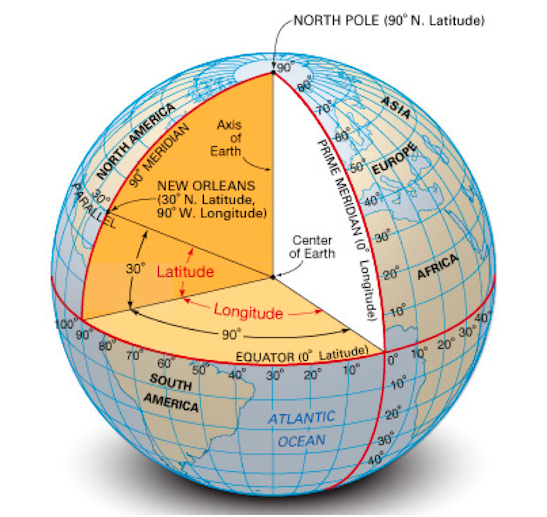
\includegraphics[width=5cm]{Longitude_latitude}
\end{debat}

\hfill {\gray Vidéo : \href{https://www.youtube.com/watch?v=lpYEuHeecko}{{\bf Les fondamentaux : latitude et longitude}, chaîne YouTube {\it La Classe d'Histoire}.}}


%%% Activité d'approche %%%
\begin{Maquette}[Cours]{Theme={Activité d'approche},Couleur={SteelBlue}}

   \AAtitre{Couples d'angles}
      {\it Objectifs : faire découvrir la notion d'angles-internes et d'angles correspondants.}

      \begin{AActivite}

         \begin{minipage}{10cm}
            \AApartie{Introduction}
               En utilisant les trois bandelettes modélisant trois droites $(d_1), (d_2)$ et $\Delta$ reliées entre elles par des attaches parisiennes, combien d'angles peut-on observer ? \pointilles
         \end{minipage}
         \hfill
         \begin{minipage}{6cm}
            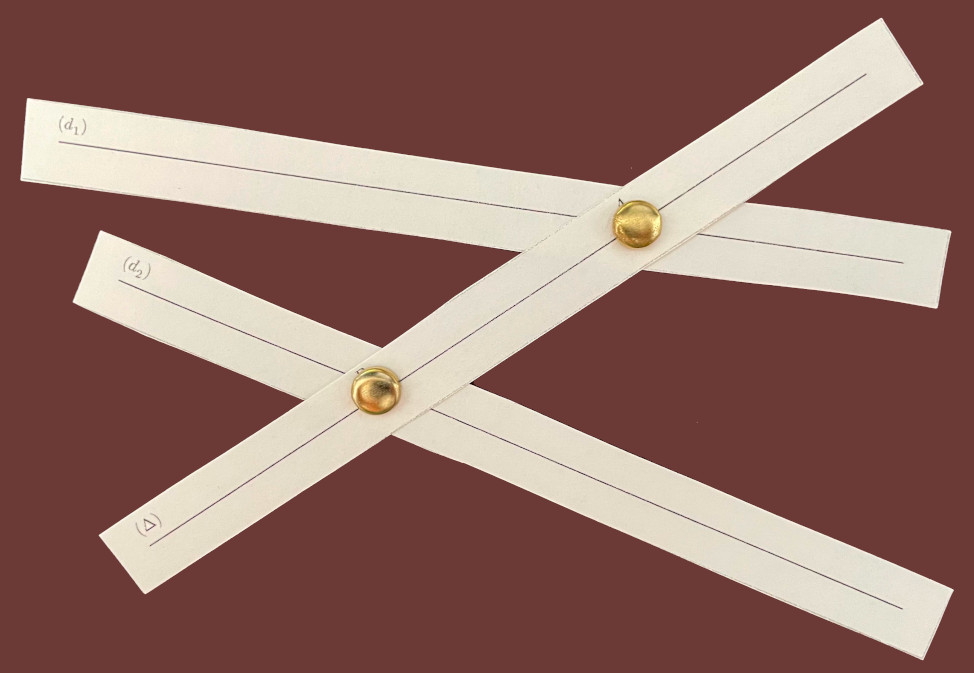
\includegraphics[width=6cm]{bandelettes}
         \end{minipage}

         \AApartie{Angles alternes-internes}
            \begin{enumerate}
               \item Prendre deux jetons, les placer sur deux angles vérifiant les conditions suivantes :
                  \begin{itemize}
                     \item les deux angles n'ont pas le même sommet ;
                     \item ils sont situés de part et d'autre de la droite $(\Delta)$ ;
                     \item ils sont situés \og entre \fg{} les droites $(d_1)$ et $(d_2)$.
                  \end{itemize}
                  Quelle est la mesure en degrés de chacun de ces deux angles ? \pointilles
               \item Combien y a-t-il de telles paires d'angles ? \pointilles \par
                  {\bf Les angles ainsi construits sont dit alternes-internes}.
               \item Placer les bandelettes de telle sorte que les droites $(d_1)$ et $(d_2)$ soient parallèles, repérer deux angles alternes-internes par deux jetons puis donner la mesure de chacun de ces deux angles. \pointilles
               \item En observant les résultats de la classe, quelle conjecture peut-on faire ? \par
                  \pointilles
            \end{enumerate}

         \AApartie{Angles correspondants}
            \begin{enumerate}[resume]
               \item Prendre deux jetons, les placer sur deux angles vérifiant les conditions suivantes :
                  \begin{itemize}
                     \item les deux angles n'ont pas le même sommet ;
                     \item ils sont situés du même côté que la droite $(\Delta)$ ;
                     \item l'un est situé \og entre \fg{} les droites $(d_1)$ et $(d_2)$, l'autre à l'extérieur.
                  \end{itemize}
                  Quelle est la mesure en degrés de chacun de ces deux angles ? \pointilles
               \item Combien y a-t-il de telles paires d'angles ? \pointilles \par
                  {\bf Les angles ainsi construits sont dit correspondants}.
               \item Placer les bandelettes de telle sorte que les droites $(d_1)$ et $(d_2)$ soient parallèles, repérer deux angles alternes-internes par deux jetons puis donner la mesure de chacun de ces deux angles. \pointilles
               \item En observant les résultats de la classe, quelle conjecture peut-on faire ? \par
                  \pointilles
            \end{enumerate}

      \end{AActivite}

\end{Maquette}


%%% Trace écrite %%%
\begin{Maquette}[Cours]{Theme={Trace écrite},Couleur={0.4[SteelBlue,Black]}}
   
   %%% 1
   \section{Mesure d'angles particuliers : rappels}

      \begin{minipage}{10.5cm}
         \begin{pspicture}(-5.5,-0.75)(5,2.5)
            \rput(0,-0.3){O}
            \rput(3.8,0){angle nul : 0°}
            \pswedge[fillstyle=solid,fillcolor=Crimson,linecolor=Crimson](0,0){1.5}{0}{90}
            \rput(2.5,1.3){\parbox{2.1cm}{\textcolor{Crimson}{angle aigu : \\ 0° < \pswedge[fillstyle=solid,fillcolor=Crimson,linecolor=Crimson](0.2,0){0.3}{0}{90} \qquad < 90°}}}
            \pswedge[fillstyle=solid,fillcolor=DodgerBlue,linecolor=DodgerBlue](0,0){1.5}{90}{180}
            \rput(-2.5,1.3){\parbox{2.5cm}{\textcolor{DodgerBlue}{angle obtus : \\ 90° < \pswedge[fillstyle=solid,fillcolor=DodgerBlue,linecolor=DodgerBlue](0.4,0){0.3}{90}{180} \quad\; < 180°}}}
            \rput(0,2.3){angle droit : 90°}
            \rput(-3.8,0){angle plat : 180°}
            \psline(-2.5,0)(2.5,0)
            \psline(0,2)
         \end{pspicture}   
      \end{minipage}
      \qquad
      \begin{minipage}{6cm}
         Dans cette configuration, la somme des deux angles mesure 180°, on dit que ces angles sont supplémentaires. \par
         \begin{pspicture}(0,-0.25)(6,1.5)
            \psline(0.5,0)(5.5,0)
            \psline(3,0)(1.8,1.2)
            \psarc[linecolor=Crimson](3,0){0.7}{135}{180}
            \rput(2,0.4){\textcolor{Crimson}{45°}}
            \psarc[linecolor=DodgerBlue](3,0){0.5}{0}{135}
            \rput(3.6,0.7){\textcolor{DodgerBlue}{135°}}
         \end{pspicture}
      \end{minipage}
   

   %%% 2
   \section{Angles alternes-internes et correspondants}
   
      \begin{minipage}{9cm}
         Lorsque deux droites sont coupées par une droite sécante $(\Delta)$, on obtient huit angles. \par
         {\it Dans la suite du cours, on se place dans cette configuration.}
      \end{minipage}
      \hfill 
      \begin{minipage}{6.5cm}
         \psset{unit=0.7}
         \begin{pspicture}(-1,-1)(6,3.5)
            \psline(0,1.5)(6,0.5)
            \psline(1,3)(6,3)
            \psline(1,0)(5,4)
            \psarc[linecolor=Crimson,doubleline=true](4,3){0.7}{0}{45}
            \rput(5,3.4){\textcolor{Crimson}{\small $A_2$}}
            \psarc[linecolor=DarkOrange,doubleline=true](4,3){0.7}{180}{225}
            \rput(3,2.5){\textcolor{DarkOrange}{\small $A_4$}}
            \psarc[linecolor=DodgerBlue](4,3){0.5}{45}{180}
            \rput(3.7,3.8){\textcolor{DodgerBlue}{\small $A_1$}}
            \psarc[linecolor=ForestGreen](4,3){0.5}{225}{0}
            \rput(4.35,2.25){\textcolor{ForestGreen}{\small $A_3$}}
            \psarc[linecolor=Crimson,doubleline=true](2.15,1.15){0.7}{-10}{45}
            \rput(3.2,1.4){\textcolor{Crimson}{\small $B_2$}}
            \psarc[linecolor=DarkOrange,doubleline=true](2.15,1.15){0.7}{170}{225}
            \rput(1.1,0.7){\textcolor{DarkOrange}{\small $B_4$}}
            \psarc[linecolor=DodgerBlue](2.15,1.15){0.5}{45}{170}
            \rput(1.8,1.9){\textcolor{DodgerBlue}{\small $B_1$}}
            \psarc[linecolor=ForestGreen](2.15,1.15){0.5}{225}{-10}
            \rput(2.4,0.3){\textcolor{ForestGreen}{\small $B_3$}}
            \rput(0.7,-0.3){$(\Delta)$}
            \rput(-0.5,1.5){$(d_1)$}
            \rput(0.5,3){$(d_2)$}
         \end{pspicture}
      \end{minipage}
      
      \begin{definition*}{}
         Deux angles sont {\bf alternes-internes} s'ils n'ont pas le même sommet, qu'ils sont situés de part et d'autre de la sécante $(\Delta)$ et qu'ils se situent \og entre \fg{} les droites $(d_1)$ et $(d_2)$.
      \end{definition*}
      
      \begin{exemple*}{}
         Sur la figure, il y a deux couples d'angles alternes-internes : $A_4$ et $B_2$ ; $A_3$ et $B_1$.
      \end{exemple*}
      
      \begin{definition*}{}
         Deux angles sont {\bf correspondants} s'ils n'ont pas le même sommet, qu'ils sont situés du même côté de la sécante $(\Delta)$, l'un entre les deux droites $(d_1)$ et $(d_2)$ et l'autre à l'extérieur.
      \end{definition*}
      
      \begin{exemple*}{}
         Sur la figure, il existe quatre couples d'angles correspondants :  $A_1$ et $B_1$ ; $A_2$ et $B_2$ ; $A_3$ et $B_3$ ; $A_4$ et $B_4$.
      \end{exemple*}
      
    
   %%%% 3
   \section{Et si les droites sont parallèles ?}
   
   \begin{propriete*}{}
      \begin{itemize}
         \item Si les deux droites $(d_1)$ et $(d_2)$ sont parallèles, alors les angles alternes-internes et les angles correspondants sont égaux deux à deux.
         \item Si deux angles alternes-internes ou deux angles correspondants sont égaux, alors les droites $(d_1)$ et $(d_2)$ sont parallèles.
      \end{itemize}
   \end{propriete*}
   
   \begin{exemple*}{}
      \begin{minipage}{6cm}
         \psset{unit=0.9}
         \begin{pspicture}(0,0.3)(6,3.2)
            \psline(1,1)(6,1)
            \psline(1,2.5)(6,2.5)
            \psline(2,0)(4,3)
            \rput(2.4,2.1){$\alpha =56°$}
            \rput(3.5,1.5){$\beta$}
            \rput(1.8,0.5){$\gamma$}
            \psarc[linecolor=Crimson,doubleline=true](3.67,2.5){0.6}{182}{234}
            \psarc[linecolor=DodgerBlue,doubleline=true](2.67,1){0.6}{2}{55}
            \psarc[linecolor=DarkOrange,doubleline=true](2.67,1){0.6}{182}{233}
            \rput(5.5,1.75){\parbox{1.5cm}{\small droites\\parallèles}}
         \end{pspicture}
      \end{minipage}
      \qquad
      \begin{minipage}{10cm}
         Mesures de $\beta$ et $\gamma$, sachant que les droites sont parallèles :
         \begin{itemize}
            \item $\alpha$ et $\beta$ sont des angles alternes-internes, ils ont donc même mesure. D'où : $\beta =\alpha =56°$.
            \item $\alpha$ et $\gamma$ sont des angles correspondants, ils ont donc même mesure. D'où : $\gamma =\alpha =56°$.
         \end{itemize}
      \end{minipage}
   \end{exemple*}

\end{Maquette}


%%% Exercices %%%
\begin{Maquette}[Fiche,CorrigeFin,Colonnes=2]{}

   \begin{multicols}{2}

      \begin{exercice} %1
         Au regard de la figure, que peut-on dire des angles :
         \begin{colenumerate}[3]%
            \item 1 et 5 ?
            \item 2 et 6 ?
            \item 4 et 6 ?
            \item 3 et 7 ?
            \item 3 et 5 ?
            \item 4 et 8 ?
         \end{colenumerate}
         {\psset{unit=0.7}
         \begin{pspicture}(-1.5,0)(6,4.5)
            \psline(0,1.5)(6,0.5)
            \psline(1,3)(6,3)
            \psline(1,0)(5,4)
            \psarc(4,3){0.7}{0}{45}
            \rput(5,3.4){2}
            \psarc(4,3){0.7}{180}{225}
            \rput(3,2.5){4}
            \psarc(4,3){0.5}{45}{180}
            \rput(3.7,3.8){1}
            \psarc(4,3){0.5}{225}{0}
            \rput(4.35,2.25){3}
            \psarc(2.15,1.15){0.7}{-10}{45}
            \rput(3.2,1.4){6}
            \psarc(2.15,1.15){0.7}{170}{225}
            \rput(1.1,0.7){8}
            \psarc(2.15,1.15){0.5}{45}{170}
            \rput(1.8,1.9){5}
            \psarc(2.15,1.15){0.5}{225}{-10}
            \rput(2.4,0.3){7}
         \end{pspicture}}
      \end{exercice}

      \begin{Solution}
         \begin{enumerate}
            \item Les angles 1 et 5 sont \cor{correspondants}.
            \item Les angles 2 et 6 sont \cor{correspondants}.
            \item Les angles 4 et 6 sont \cor{alternes-internes}.
            \item Les angles 3 et 7 sont \cor{correspondants}.
            \item Les angles 3 et 5 sont \cor{alternes-internes}.
            \item Les angles 4 et 8 sont \cor{correspondants}.
         \end{enumerate}
      \end{Solution}
      
      
      \begin{exercice} %2
         Dans la configuration suivante, citer :
         \begin{enumerate}
               \item la sécante ;
               \item deux angles correspondants ;
               \item deux angles alternes-internes.
         \end{enumerate}
         {\psset{unit=0.9}
         \begin{pspicture}(-3,-1.5)(3,1.2)
            \psline(-1.5,0)(2,0)
            \psline(-1,0.75)(2,-1.5)
            \psline(-1.5,-1)(2.5,-1)
            \rput(-1.75,0){$x$}
            \rput(-1.2,0.9){$y$}
            \rput(2.25,0){$t$}
            \rput(2.25,-1.6){$s$}
            \rput(2.75,-1){$u$}
            \rput(0.2,0.25){$O$}
            \rput(1.5,-0.75){$I$}
            \rput(-1.75,-1){$k$}
         \end{pspicture}}
      \end{exercice}

      \begin{Solution}
         \begin{enumerate}
            \item La sécante est \cor{la droite $(ys)$}.
            \item Il y a quatre couples d'angles correspondants : \par
               \cor{$\widehat{yOt}$ et $\widehat{OIu}$} ; \par
               \cor{$\widehat{yOx}$ et $\widehat{OIk}$} ; \par
               \cor{$\widehat{tOI}$ et $\widehat{uIs}$} ; \par
               \cor{$\widehat{xOI}$ et $\widehat{kIs}$}.
            \item Il y a deux couples d'angles alternes-internes : \par
               \cor{$\widehat{xOI}$ et $\widehat{OIu}$} \par
               \cor{$\widehat{tOI}$ et $\widehat{OIk}$}.
         \end{enumerate}
      \end{Solution}
      
      
      \begin{exercice}[Tout] %3
         Sur cette figure, les droites $(xy)$ et $(zt)$, ainsi que les droites $(su)$ et $(fg)$, sont parallèles. \par
         Compléter le tableau suivant lorsque c'est possible.
         \begin{center}
            \psset{xunit=1.8cm,yunit=0.8cm}
            \begin{pspicture}(-1.25,-2.2)(2.25,1.2)
               \psline(-1,0)(2,0)
               \psline(-1,-1)(2,-1)
               \psline(-1,1)(1,-2)
               \psline(0,1)(2,-2)
               \psline(0,-2)(1,1)
               \rput(-1.1,0){$x$}
               \rput(2.1,0){$y$}
               \rput(-1.1,-1){$z$}
               \rput(2.1,-1){$t$}
               \rput(-1.1,1.1){$s$}
               \rput(1.1,-2.1){$u$}
               \rput(-0.1,1.1){$f$}
               \rput(2.1,-2.1){$g$}      
               \rput(-0.1,-2.1){$h$}
               \rput(1.1,1.1){$i$}
               \rput(-0.3,0.25){$A$}
               \rput(0.85,0.2){$B$}
               \rput(0.3,-0.65){$C$}
               \rput(1.4,-0.65){$D$}
            \end{pspicture}
         \end{center}
         \begin{tabular}{|C{2.2}|*{4}{C{0.8}|}}
            \hline
            angle & $\widehat{yBg}$ & $\widehat{zCi}$ & $\widehat{fBi}$ & $\widehat{uCi}$ \\
            \hline
            alterne-interne & & & & \\
            \hline
            correspondant & & & & \\
            \hline
         \end{tabular}
      \end{exercice}

      \begin{Solution}
         On obtient le tableau suivant, par exemple : \par \smallskip
         {\hautab{2}
         \begin{tabular}{|C{1.8}|*{4}{C{0.85}|}}
            \hline
            angle & $\widehat{yBg}$ & $\widehat{zCi}$ & $\widehat{fBi}$ & $\widehat{uCi}$ \\
            \hline
            \footnotesize Angles alterne-interne & \textcolor{RoyalBlue}{$\widehat{zDf}$ $\widehat{BDC}$\dots} & \textcolor{RoyalBlue}{$\widehat{hBy}$ $\widehat{yBC}$\dots} & \textcolor{RoyalBlue}{$\varnothing$} & \textcolor{RoyalBlue}{$\widehat{fBh}$ $\widehat{CBf}$\dots} \\
            \hline
            \footnotesize Angles correspondant & \textcolor{RoyalBlue}{$\widehat{tDg}$ $\widehat{yAu}$\dots} & \textcolor{RoyalBlue}{$\widehat{xBi}$ $\widehat{iBA}$\dots} & \textcolor{RoyalBlue}{$\widehat{sCi}$ $\widehat{BCA}$\dots} & \textcolor{RoyalBlue}{$\widehat{gBi}$ $\widehat{iBD}$\dots} \\
            \hline
         \end{tabular}}
      \end{Solution}
      
      
      \begin{exercice} %4
         Batoul pense que l'une des deux paires de droites $(d_1)$ et $(d_2)$ est parallèle. A-t-elle raison ? Justifier \par
         {\psset{unit=0.8}
         \begin{pspicture}(0.2,-0.2)(4,2.5)
            \pstGeonode[PointSymbol=none,PointName=none](0,2.5){A}(4,0){B}(0,1){C}(3,2){D}(1,0){E}(4,1){F}
            \pstInterLL[PointName=none,PointSymbol=none]{A}{B}{C}{D}{H}
            \pstInterLL[PointName=none,PointSymbol=none]{A}{B}{E}{F}{I}
            \pstLineAB{A}{B}
            \pstLineAB{C}{D}
            \pstLineAB{E}{F}
            \pstMarkAngle{D}{H}{A}{119°}
            \pstMarkAngle{B}{I}{F}{61°}
            \rput(0.5,0.8){$(d_1)$}
            \rput(1.7,-0.2){$(d_2)$}
         \end{pspicture} 
         \begin{pspicture}(-1,-0.2)(3.3,3.2)
            \pstGeonode[PointSymbol=none,PointName=none](0,1.5){A}(3,1){B}(0,0){C}(1.5,3){D}(1.5,0){E}(2.5,2.5){F}
            \pstInterLL[PointName=none,PointSymbol=none]{A}{B}{C}{D}{H}
            \pstInterLL[PointName=none,PointSymbol=none]{A}{B}{E}{F}{I}
            \pstLineAB{A}{B}
            \pstLineAB{C}{D}
            \pstLineAB{E}{F}
            \pstMarkAngle{B}{H}{D}{59°}
            \pstMarkAngle{E}{I}{B}{111°}
            \rput(1,2.8){$(d_1)$}
            \rput(3,2.5){$(d_2)$}
         \end{pspicture}}
      \end{exercice}

      \begin{Solution}
         Oui, Batoul a raison : \par
         \begin{itemize}
            \item Première figure : l'angle supplémentaire à 119° de l'autre côté de $(d_1)$ vaut $180°-119° =61°$. \par
               On a deux angles correspondants de même mesure donc, \cor{les droites $(d_1)$ et $(d_2)$ sont parallèles}.
            \item Deuxième figure : l'angle supplémentaire à 111° de l'autre côté de $(d_2)$ vaut $180°-111° =69°$. \par
               On a deux angles alternes-internes de mesures différentes donc, \cor{$(d_1)$ et $(d_2)$ ne sont pas parallèles}.
         \end{itemize}
      \end{Solution}
      
      
      \begin{exercice} %5
         Dans la figure ci-dessous, on sait que les droites $(xy)$ et $(tz)$ sont parallèles et on connaît la mesure de deux angles. En utilisant les données de la figure :
         \begin{enumerate}
            \item Donner la mesure en degrés d'un maximum d'angles de la figure.
            \item En déduire la nature du triangle $IJK$?
         \end{enumerate}
         \begin{pspicture}(-2,-0.5)(4.8,3)
            \pstGeonode[PointSymbol=none,PosAngle={180,120,-120,0,180,0}](-1,0){z}(0,0){K}(2,0){J}(4,0){t}
            \pstRotation[PointSymbol=none,PosAngle=150,RotAngle=60]{K}{J}[I]
            \pstOIJGeonode[PointSymbol=none,PosAngle={180,0,60,120}](-1,1){x}{K}{J}{I}(1.5,1){y}(0,1.4){s}(-.4,1.4){r}
            \pstLineAB{x}{y}
            \pstLineAB{z}{t}
            \pstLineAB[nodesepA=-.9,nodesepB=-.5]{I}{K}
            \pstLineAB[nodesepA=-.9, nodesepB=-.5]{I}{J}
            \pstMarkAngle{t}{J}{r}{120°}
            \pstMarkAngle{y}{I}{s}{60°}
         \end{pspicture}
      \end{exercice}

      \begin{Solution}
         \begin{enumerate}
            \item $\bullet$ Les angles $\widehat{IJK}$ et $\widehat{IJt}$ sont supplémentaires \par
               donc, $\cor{\widehat{IJK}} =180°-120°° =\cor{60°}$. \par
               $\bullet$ Les angles $\widehat{JKI}$ et $\widehat{yIS}$ sont correspondants et $\widehat{yIS} =60°$ \par
               donc, \cor{$\widehat{JKI} =60°$}. \par
               $\bullet$ Les angles $\widehat{rIy}$ et $\widehat{IJt}$ sont correspondants et $\widehat{IJt} =120°$ \par
               donc, \cor{$\widehat{rIy} =120°$}. \par
               $\bullet$ Les angles $\widehat{yIJ}$ et $\widehat{rIy}$ sont supplémentaires \par
               donc, $\cor{\widehat{yIJ}} =180°-120°° =\cor{60°}$. \par
               $\bullet$ Les angles $\widehat{xIK}$ et $\widehat{sIy}$ sont opposés par le sommet \par
               donc, $\cor{\widehat{xIK}} =\widehat{sIy} =\cor{60°}$. Et enfin : \par
               $\cor{\widehat{KIJ}} =180° -\widehat{xIK}-\widehat{yIJ}$ \par
               $=180°-60°-60° =\cor{60°}$.
            \item Les trois angles du triangle sont égaux, donc \cor{le triangle $IJK$ est équilatéral}.
         \end{enumerate}
      \end{Solution}
      
      
      \begin{exercice}[Dur] %6
         Sur la figure ci-dessous :
         \begin{itemize}
            \item les droites $(ab), (cd)$ et $(ef)$ sont parallèles ;
            \item $R$ est un point de $(ab)$, $S$ un point de $(cd)$ et $T$ un point de $(ef)$ tels que $\widehat{bRS} =20°$ et $\widehat{RST} =57°$.
         \end{itemize}
         Calculer la mesure de l'angle $\widehat{STf}$. \par
         \begin{pspicture}(-0.5,0.2)(7,3.8)
            \pstGeonode[PointSymbol=none,PosAngle={90}](0,0.5){e}(2,0.5){T}(7,0.5){f}(0,2){c}(4,2){S}(7,2){d}(0,3){a}(2,3){R}(7,3){b}
            \pstLineAB{a}{b}
            \pstLineAB{c}{d}
            \pstLineAB{e}{f}
            \pstLineAB{R}{S}
            \pstLineAB{S}{T}
            \pstMarkAngle{S}{R}{b}{}
            \rput(3,2.8){20°}
            \pstMarkAngle[MarkAngleType=double]{R}{S}{T}{}
            \rput(3.2,1.8){57°}
            \pstMarkAngle{f}{T}{S}{?}
         \end{pspicture}
      \end{exercice}

      \begin{Solution}
         \begin{itemize}
            \item Les angles $\widehat{bRS}$ et $\widehat{RSc}$ sont alternes-internes et les droites $(ab)$ et $(cd)$ sont parallèles donc : $\widehat{RSc} =\widehat{bRS} =20°$.
            \item On décompose l'angle $\widehat{RST}$ : $\widehat{RST} =\widehat{RSc}+\widehat{cST}$ donc, $\widehat{cST} =\widehat{RST} -\widehat{RSc} =57°-20° =37°$.
            \item Les angles $\widehat{cST}$ et $\widehat{STf}$ sont alternes-internes et les droites $(cd)$ et $(ef)$ sont parallèles donc : $\widehat{STf} =\widehat{cST} =\blue 37°$.
         \end{itemize}
      \end{Solution}
      
      
      \begin{exercice}[Dur] %7
         Léon possède un champ en forme de quadrilatère $LEON$ dont les côtés $(LE)$ et $(ON)$ sont parallèles. Il prend la mesure de deux angles et se demande si son quadrilatère peut être un parallélogramme.
         \begin{enumerate}
            \item Écrire sur le schéma ci-dessous la mesure de tous les angles existants.
            \item Les droites $(LN)$ et $(EO)$ sont-elles parallèles ?
            \item Quelle est alors la nature du quadrilatère $LEON$ ?
         \end{enumerate}
         {\psset{unit=0.6}
         \begin{pspicture}(-1,0)(10,6)
            \pstGeonode[PointSymbol=none,PointName=none](0,1){a}(10,1){b}(0,4){c}(10,4){d}(0.33,0){f}(4,5.5){g}(6.33,0){h}(9,5){j}
            \pstLineAB{a}{b}
            \pstLineAB{c}{d}
            \pstLineAB{f}{g}
            \pstLineAB{h}{j}
            \pstInterLL[PosAngle=-45,PointSymbol=none]{a}{b}{f}{g}{N}
            \pstInterLL[PosAngle=-45,PointSymbol=none]{a}{b}{h}{j}{O}
            \pstInterLL[PosAngle=-45,PointSymbol=none]{c}{d}{f}{g}{L}
            \pstInterLL[PosAngle=-45,PointSymbol=none]{c}{d}{h}{j}{E}
            \pstMarkAngle{j}{E}{L}{121°}
            \pstMarkAngle{O}{N}{L}{49°}
         \end{pspicture}}
      \end{exercice}
      
      \begin{Solution}
         \begin{enumerate}
            \item Schéma du terrain de Léon : \par
               {\psset{unit=0.7}
               \begin{pspicture}(-0.5,-0.5)(10,6)
                  \pstGeonode[PointSymbol=none,PointName=none](0,1){a}(10,1){b}(0,4){c}(10,4){d}(0.33,0){f}(4.5,5.5){g}(6.33,0){h}(9,5){j}
                  \pstLineAB{a}{b}
                  \pstLineAB{c}{d}
                  \pstLineAB{f}{g}
                  \pstLineAB{h}{j}
                  \pstInterLL[PosAngle=-45,PointSymbol=none,PointName=none]{a}{b}{f}{g}{S}
                  \pstInterLL[PosAngle=-45,PointSymbol=none,PointName=none]{a}{b}{h}{j}{E}
                  \pstInterLL[PosAngle=-45,PointSymbol=none,PointName=none]{c}{d}{f}{g}{I}
                  \pstInterLL[PosAngle=-45,PointSymbol=none,PointName=none]{c}{d}{h}{j}{N}
                  \pstMarkAngle{j}{N}{I}{121°}
                  \pstMarkAngle{E}{S}{I}{49°}
                  \pstMarkAngle{I}{N}{E}{\cor{59°}}
                  \pstMarkAngle{E}{N}{d}{\cor{121°}}
                  \pstMarkAngle{d}{N}{j}{\cor{59°}}
                  \pstMarkAngle{b}{E}{N}{\cor{59°}}
                  \pstMarkAngle{h}{E}{b}{\cor{121°}}
                  \pstMarkAngle{N}{E}{S}{\cor{121°}}
                  \pstMarkAngle{S}{E}{h}{\cor{59°}}
                  \pstMarkAngle{f}{S}{E}{\cor{131°}}
                  \pstMarkAngle{I}{S}{a}{\cor{131°}}
                  \pstMarkAngle{a}{S}{f}{\cor{49°}}
                  \pstMarkAngle{f}{S}{E}{\cor{131°}}
                  \pstMarkAngle{I}{S}{a}{\cor{131°}}
                  \pstMarkAngle{g}{I}{e}{\cor{131°}}
                  \pstMarkAngle{e}{I}{f}{\cor{49°}}
                  \pstMarkAngle{d}{I}{g}{\cor{49°}}
                  \pstMarkAngle{f}{I}{d}{\cor{131°}}
               \end{pspicture}}
            \item Si les droites $(LN)$ ET $(EO)$ étaient parallèles, les angles correspondants en $L$ et $E$ par exemple seraient égaux, ce qui n'est pas le cas ici (131°$\neq$121°) donc, \cor{ces droites ne sont pas parallèles}.
            \item Dans le quadrilatère $LEON$, les droites $(LE)$ et $(ON)$ sont parallèles, mais les droites $(LN)$ et $(EO)$ ne le sont pas donc, \cor{le quadrilatère $LEON$ est un trapèze}.   
         \end{enumerate}
      \end{Solution}
      
   \end{multicols}

\end{Maquette}


%%% Récréation %%%
\begin{Maquette}[Cours]{Theme={Activité récréative},Couleur={IndianRed}} %maquette d'activité récréative
    
   \ARtitre{Le flexagone}

      \ARpartie{Construction du flexagone}
         \begin{enumerate}
            \item Reproduire, puis découper la figure ci-dessous, composée de 9 triangles équilatéraux de côté 5 cm. 
               \begin{center}
                  \psset{unit=0.6}
                  \begin{pspicture}(0,0)(10,2)
                     \multido{\n=0+2}{5}{\rput(\n,0){\pspolygon(0,0)(2,0)(2;60)}}
                     \psline(2;60)(9,1.732)
                  \end{pspicture}
               \end{center}
            \item Marquer le pli vallée au niveau de l'arête commune entre le 3\up{e} et le 4\up{e} triangle, puis replier vers le haut les trois premiers triangles.
               \begin{center}
                  \psset{unit=0.6}
                  \begin{pspicture}(3,0)(10,3)
                     \multido{\n=4+2}{3}{\rput(\n,0){\pspolygon(0,0)(2,0)(2;60)}}
                     \pspolygon[fillstyle=solid,fillcolor=lightgray](4,0)(3,1.732)(4,3.464)(6,3.464)(6,3.464)
                     \psline(3,1.732)(9,1.732)
                     \psline(4,3.464)(5,1.732)
                  \end{pspicture}
               \end{center}
            \item Marquer le pli montagne au niveau de l'arête commune entre le 6\up{e} et le 7\up{e} triangle, puis replier vers le haut les trois derniers triangles en faisant passer le dernier triangle sur le premier triangle.
               Enfin, mettre un morceau de ruban adhésif pour maintenir le premier et le dernier triangle ensemble. \par
               \begin{center}
                  \psset{unit=0.6}
                  \begin{pspicture}(3,0)(13,4.5)
                     \rput(4,0){\pspolygon(0,0)(2,0)(2;60)}
                     \pspolygon[fillstyle=solid,fillcolor=lightgray](4,0)(3,1.732)(4,3.464)(6,3.464)(6,3.464)
                     \psline(3,1.732)(7,1.732)
                     \psline(4,3.464)(5,1.732)
                     \psline(6,0)(7,1.732)
                     \pspolygon[fillstyle=solid,fillcolor=gray](5,1.732)(7,1.732)(6,3.464)
                     \psline{->}(8,3)(12,3)
                     \rput(10,3.5){\it\small passer le dernier}
                     \rput(10,2.5){\it\small triangle au dessus}
                  \end{pspicture}
                  \begin{pspicture}(3,0)(7,4.5)
                     \rput(4,0){\pspolygon(0,0)(2,0)(2;60)}
                     \pspolygon[fillstyle=solid,fillcolor=lightgray](4,0)(3,1.732)(4,3.464)(6,3.464)
                     \pspolygon[fillstyle=solid,fillcolor=gray](5,1.732)(7,1.732)(6,3.464)(4,3.464)
                     \psline(3,1.732)(7,1.732)(6,0)
                     \psline(5,1.732)(6,3.464)   
                     \rput(5,4.5){\it scotch} 
                     \psline{->}(5,4.2)(5,3.7)    
                  \end{pspicture}
            \end{center}
         \end{enumerate}

      \ARpartie{Utilisation du flexagone}
         \begin{enumerate}
            \item On obtient un hexagone, ou plus précisément un hexaflexagone. Dessiner ou colorier les deux faces obtenues.
            \item Marquer tous les plis dans les deux sens.
            \item Plier une arête sur deux en alternant les plis vallée et montagne de telle sorte que les soufflets soient en plis montagne, puis ouvrir : on obtient, de manière magique, une troisième face que l'on peut à son tour colorier. \medskip
               \begin{center}
                  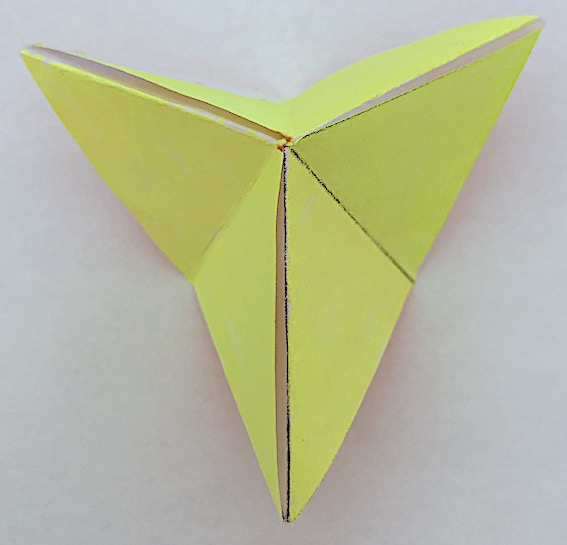
\includegraphics[height=3cm]{flexagone1} 
                  \qquad
                  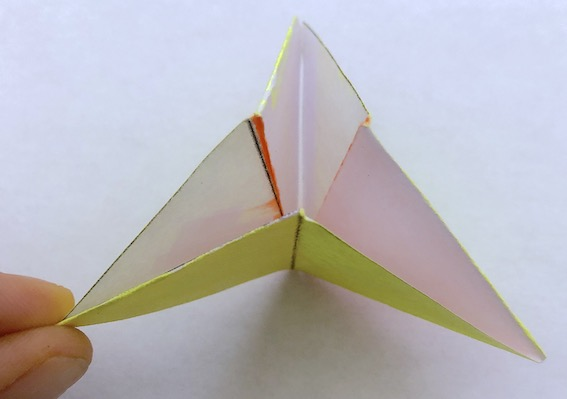
\includegraphics[height=3cm]{flexagone2} 
               \end{center}
            \item En réitérant le pliage, on obtient successivement les trois faces, une à une.
         \end{enumerate}
   
      \ARpartie{Pour aller plus loin}
         \begin{itemize}
            \item Un article, paru dan le magasine \og Pour la science \fg{} et écrit par {\it Jean-Paul Delahaye}, explique que l'on peut faire des flexagones avec autant de faces que l'on souhaite : \href{https://www.cristal.univ-lille.fr/~jdelahay/pls/2005/131.pdf}{\og Flexagones \fg}
            \item Il existe également des sites spécialisés, comme \href{http://www.flexagon.net}{Flexagone.net} qui propose de multiples modèles décorés à imprimer 
         \end{itemize}

\end{Maquette}
    \pagebreak
    \graphicspath{{../../S03_En_route_vers_la_programmation/Images/}}

\themeA
\chapter{En route vers la programmation}
\label{S03}


\programme%
   {\item Notions d'algorithme et de programme. 
    \item Notion de variable informatique.
    \item Déclenchement d'une action par un événement.
    \item Séquences d'instructions, boucles, instructions conditionnelles.}
   {\item Écrire, mettre au point (tester, corriger) et exécuter un programme en réponse à un problème donné.}

\vfill

\begin{debat}{Débat : la fourmi de Langton, que se passe-t-il ensuite ?}
   La {\bf fourmi de Langton}, du nom de son inventeur scientifique américain {\it Christopher Langton}, est un petit programme informatique inventé vers la fin des années 1980. \par
   Il consiste en un automate qui se déplace dans un quadrillage suivant des règles simples. Il modélise le fait qu'un ensemble de comportements élémentaires peut donner lieu à un comportement complexe.
   \tcblower
      \psset{unit=0.2}
      \begin{pspicture}(0,0)(13,13)
         \fourmi{6.5}{6.5}{-90}
         \rput(2,0){\cub} \rput(3,0){\cub}
         \rput(1,1){\cub} \rput(2,1){\cub} \rput(9,1){\cub} \rput(10,1){\cub}
         \rput(0,2){\cub} \rput(2,2){\cub} \rput(3,2){\cub} \rput(5,2){\cub} \rput(8,2){\cub} \rput(11,2){\cub}
         \rput(0,3){\cub} \rput(3,3){\cub} \rput(5,3){\cub} \rput(6,3){\cub} \rput(7,3){\cub} \rput(9,3){\cub} \rput(10,3){\cub} \rput(11,3){\cub}
         \rput(1,4){\cub} \rput(3,4){\cub} \rput(10,4){\cub} \rput(12,4){\cub}
         \rput(3,5){\cub} \rput(4,5){\cub} \rput(8,5){\cub} \rput(9,5){\cub}
         \rput(3,6){\cub} \rput(4,6){\cub} \rput(5,6){\cub} \rput(7,6){\cub} \rput(8,6){\cub} \rput(9,6){\cub}
         \rput(3,7){\cub} \rput(4,7){\cub} \rput(8,7){\cub} \rput(9,7){\cub}
         \rput(0,8){\cub} \rput(2,8){\cub} \rput(9,8){\cub} \rput(11,8){\cub}
         \rput(0,9){\cub} \rput(1,9){\cub} \rput(2,9){\cub} \rput(5,9){\cub} \rput(6,9){\cub} \rput(7,9){\cub} \rput(9,9){\cub} \rput(12,9){\cub}
         \rput(1,10){\cub} \rput(4,10){\cub} \rput(7,10){\cub} \rput(9,10){\cub} \rput(10,10){\cub} \rput(12,10){\cub}
         \rput(2,11){\cub} \rput(3,11){\cub} \rput(10,11){\cub} \rput(11,11){\cub}
         \rput(9,12){\cub} \rput(10,12){\cub}
      \end{pspicture}
\end{debat}

\hfill {\gray Vidéo : \href{https://www.youtube.com/watch?v=qZRYGxF6D3w}{\bf La fourmi de Langton}, chaîne YouTube {\it Science étonnante}.}


%%% Approche %%%
\begin{Maquette}[Cours]{Theme={Activité d'approche},Couleur={SteelBlue}}

   \AAtitre{La fourmi de Langton}

      {\it Objectifs : suivre un algorithme de déplacement ; se repérer dans le plan dans un repérage relatif.}

      \begin{AActivite}

         \AApartie{Les règles du jeu}
            La fourmi de Langton est un automate qui se déplace dans un quadrillage suivant les règles suivantes :
            {\singlespacing
            \begin{itemize}
               \item au départ, toutes les cases sont de la même couleur, ici blanches ;
               \item si la fourmi est sur une case blanche, elle tourne de 90° vers la droite, change la couleur de la case en noir et avance d'une case ;
               \item si la fourmi est sur une case noire, elle tourne de 90° vers la gauche, change la couleur de la case en blanc et avance d'une case.
            \end{itemize}}

         \AApartie{À vous de jouer !}
            Compléter dans les quadrillages ci-dessous les quinze premières étapes du déplacement de la fourni. \par
            \begin{center}
               \psset{unit=0.5,subgriddiv=1,gridlabels=0mm,gridcolor=gray}
               \small
               \begin{pspicture}(0,-0.7)(7,7)
                  \psgrid(0,0)(7,7)
                  \fourmi{3.5}{3.5}{0}
                  \rput(3.5,-0.5){étape 0}
               \end{pspicture}
               \quad
               \begin{pspicture}(0,-0.7)(7,7)
                  \psframe[fillstyle=solid,fillcolor=darkgray](3,3)(4,4)
                  \psgrid(0,0)(7,7)
                  \fourmi{4.5}{3.5}{-90}
                  \rput(3.5,-0.5){étape 1}
               \end{pspicture}
               \quad
               \begin{pspicture}(0,-0.7)(7,7)  
                  \psframe[fillstyle=solid,fillcolor=darkgray](3,3)(5,4)
                  \psgrid(0,0)(7,7)
                  \fourmi{4.5}{2.5}{180}
                  \rput(3.5,-0.5){étape 2}
               \end{pspicture}
               \quad
               \begin{pspicture}(0,-0.7)(7,7)
                  \psgrid(0,0)(7,7)
                  \rput(3.5,-0.5){étape 3}
               \end{pspicture}
               \bigskip
               \begin{pspicture}(0,-0.7)(7,7)
                  \psframe[fillstyle=solid,fillcolor=darkgray](3,2)(5,4)
                  \psgrid(0,0)(7,7)
                  \fourmi{3.5}{3.5}{0}
                  \rput(3.5,-0.5){étape 4}
               \end{pspicture}
               \quad
               \begin{pspicture}(0,-0.7)(7,7)
                  \psgrid(0,0)(7,7)
                  \rput(3.5,-0.5){étape 5}
               \end{pspicture}
               \quad
               \begin{pspicture}(0,-0.7)(7,7)
                  \psgrid(0,0)(7,7)
                  \rput(3.5,-0.5){étape 6}
               \end{pspicture}
               \quad
               \begin{pspicture}(0,-0.7)(7,7)
                  \psframe[fillstyle=solid,fillcolor=darkgray](2,3)(3,5)
                  \pspolygon[fillstyle=solid,fillcolor=darkgray](3,2)(5,2)(5,4)(4,4)(4,3)(3,3)
                  \psgrid(0,0)(7,7)
                  \fourmi{3.5}{4.5}{-90}
                  \rput(3.5,-0.5){étape 7}
               \end{pspicture}
               \bigskip
               \begin{pspicture}(0,-0.7)(7,7)
                  \psgrid(0,0)(7,7)
                  \rput(3.5,-0.5){étape 8}
               \end{pspicture}
               \quad
               \begin{pspicture}(0,-0.7)(7,7)
                  \psgrid(0,0)(7,7)
                  \rput(3.5,-0.5){étape 9}
               \end{pspicture}
               \quad
               \begin{pspicture}(0,-0.7)(7,7)
                  \psgrid(0,0)(7,7)
                  \rput(3.5,-0.5){étape 10}
               \end{pspicture}
               \quad
               \begin{pspicture}(0,-0.7)(7,7)
                  \pspolygon[fillstyle=solid,fillcolor=darkgray](2,2)(5,2)(5,4)(4,4)(4,5)(2,5)(2,4)(3,4)(3,3)(2,3)
                  \psgrid(0,0)(7,7)
                  \rput(3.5,-0.5){étape 11}
                  \fourmi{1.5}{2.5}{90}
               \end{pspicture}
               \bigskip
               \begin{pspicture}(0,0)(7,7)
                  \psgrid(0,0)(7,7)
                  \rput(3.5,-0.5){étape 12}
               \end{pspicture}
               \quad
               \begin{pspicture}(0,0)(7,7)
                  \psgrid(0,0)(7,7)
                  \rput(3.5,-0.5){étape 13}
               \end{pspicture}
               \quad
               \begin{pspicture}(0,0)(7,7)
                  \psgrid(0,0)(7,7)
                  \rput(3.5,-0.5){étape 14}
               \end{pspicture}
               \quad
               \begin{pspicture}(0,0)(7,7)
                  \psgrid(0,0)(7,7)
                  \rput(3.5,-0.5){étape 15}
               \end{pspicture} 
            \end{center}

      \end{AActivite}

\end{Maquette}


%%% Trace écrite %%%
\begin{Maquette}[Cours]{Theme={Trace écrite},Couleur={0.4[SteelBlue,Black]}}

   %%% 1
   \section{Algorithmes et langages de programmation}

      \begin{definition*}{}
         Un {\bf algorithme} est une liste ordonnée et logique d'instructions permettant de réaliser une tâche de manière automatisée.
      \end{definition*}
   
      Un algorithme peut-être traduit, grâce à un langage de programmation, en un programme exécutable par un ordinateur. Ce langage peut être formel, textuel, visuel\dots{} Actuellement, le logiciel utilisé au collège est Scratch, développé par le MIT. Les programmes sont créés grâce à une succession de blocs, chacun ayant une fonction.
      \begin{center}
         \includegraphics[width=17cm]{Interface_Scratch}
      \end{center}
   
   
   %%% 2
   \section{Se déplacer}
   
      \begin{methode*}{Langages de déplacement}
         Pour se déplacer dans le plan, il existe principalement deux langages de déplacement :
         \begin{itemize}
            \item le langage {\bf absolu} composé de mots de vocabulaire du type : \og haut \fg{}, \og bas \fg{}, \og droite \fg{} et \og gauche \fg. Le déplacement se fait comme si on se plaçait en vue du dessus ;
            \item le langage {\bf relatif} composé de mots de vocabulaire du type : \og avancer \fg{}, \og tourner à droite \fg{} et \og tourner à gauche \fg. C'est ici le point de vue de l'observateur qui est adopté.
         \end{itemize}
         \begin{exmethode}
            Coder ce déplacement :
            \begin{center}
               \psset{unit=0.7}
               \begin{pspicture}(0,-1)(5,4)
                  \psgrid[subgriddiv=1,gridlabels=0mm](0,-1)(5,4)
                  \psset{linecolor=DodgerBlue,arrowsize=3mm,linewidth=0.5mm}
                  \psdots(0.5,0.5)(3.5,2.5)     
                  \psline{->}(0.5,0.5)(2.5,0.5)(2.5,2.5)(3.5,2.5)
               \end{pspicture}
            \end{center}
            \tcblower
               \begin{minipage}{3.3cm}
                  {\bf Langage absolu :} \par
                  droite \par
                  droite \par
                  haut \par
                  haut \par
                  droite
               \end{minipage}
               \;
               \begin{minipage}{3.3cm}   
                  {\bf Langage relatif :} \par
                  avancer \par
                  avancer \par
                  tourner à gauche \par
                  avancer \par
                  avancer \par
                  tourner à droite \par
                  avancer
               \end{minipage}
         \end{exmethode}
      \end{methode*}

\end{Maquette}


%%% Exercices %%%%%%%
\begin{Maquette}[Fiche,CorrigeFin,Colonnes=2]{}
   
   \begin{exercice} %1
      \begin{minipage}{8cm}
         Un programme permet à un robot de se déplacer sur les cases d'un quadrillage. \par
         Chaque case atteinte est colorée en gris. Au début d'un programme, toutes les cases sont blanches, le robot se positionne sur une case de départ indiquée par un \og {\bf d} \fg{} et la colore aussitôt en gris. \par
         Le robot se déplace suivant un programme grâce à un langage absolu dont le vocabulaire est
         \begin{center}
            \og S (south) ; E (east) ; N (north) ; W (west) \fg.
         \end{center}
         On a ci-contre des exemples de programmes.
      \end{minipage}
      \qquad
      \begin{minipage}{8cm}
         \begin{tabular}{|p{1.5cm}|C{2.5}|C{2.6}|}
            \hline
            1W
            &
            Le robot avance de 1 case vers l'ouest.
            &
            {\psset{unit=0.5cm}
            \begin{pspicture}(1,0)(3,3)
               \psframe[fillstyle=solid,fillcolor=lightgray](1,1)(3,2)
               \psgrid[gridlabels=0,subgriddiv=1,gridcolor=gray](0,0)(4,3)
               \rput(2.5,1.5){\textbf{d}}
            \end{pspicture}} \\
            \hline
            2E 1W 2N
            &
            Le robot avance de 2 cases vers l'est, puis de 1 case vers l'ouest, puis de 2 cases vers le nord.
            &
            {\psset{unit=0.5cm}
            \begin{pspicture}(0,4)(5,5)
               \pspolygon[fillstyle=solid,fillcolor=lightgray](1,1)(4,1)(4,2)(3,2)(3,4)(2,4)(2,2)(1,2)
               \psgrid[gridlabels=0,subgriddiv=1,gridcolor=gray](5,5)
               \rput(1.5,1.5){\textbf{d}}
            \end{pspicture}} \\
            \hline
         \end{tabular}
      \end{minipage}
      \begin{enumerate}
         \item Voici un programme : 1W 2N 2E 4S 2W \par
            On souhaite dessiner le motif obtenu avec ce programme. Sur votre copie, réaliser ce motif en utilisant des carreaux, comme dans les exemples précédents. On marquera un \og \textbf{d} \fg{} sur la case de départ.
         \item On fait fonctionner un programme qui dessine le motif ci-contre : \par
            \begin{minipage}{10cm}
               \begin{enumerate}
                  \item Proposer un programme permettant de dessiner ce motif.
                  \item Comment pourrait-on faire évoluer l'écriture de ce programme afin qu'il soit plus compact ?
               \end{enumerate}
            \end{minipage}
            \qquad
            \begin{minipage}{5cm}
               {\psset{unit=0.5cm}
               \begin{pspicture}(-1,-1)(8,2.5)
                  \pspolygon[fillstyle=solid,fillcolor=lightgray](0,2)(1,2)(1,1)(2,1)(2,2)(3,2)(3,1)(4,1)(4,2)(5,2)(5,1)(6,1)(6,2)(7,2)(7,0)(0,0)
                  \psgrid[gridlabels=0,subgriddiv=1,gridcolor=gray](-1,-1)(8,3)
                  \rput(0.5,1.5){\textbf{d}}
               \end{pspicture}}
            \end{minipage}
      \end{enumerate}
   \end{exercice}

   \begin{Solution}
      \begin{enumerate}
         \item On obtient le \cor{dessin d'un 9} : \par
            {\psset{linecolor=white,fillstyle=solid,fillcolor=white}
            \begin{pspicture}(-1,0)(4,7.3)
               \psframe[fillcolor=lightgray](1,1)(4,6)
               \psframe(1,2)(3,3)          
               \psframe(2,4)(3,5)
               \psgrid[gridlabels=0,subgriddiv=1,gridcolor=gray](5,7)
               \rput(1.5,1.5){\textbf{d}}
            \end{pspicture}}
         \item 
         \begin{enumerate}
            \item Le motif peut être programmé grâce à la suite : \par
               \cor{1S 2E 1N 1S 2E 1N 1S 2E 1N}
            \item On peut introduire une boucle de répétition, par exemple : \cor{3$\times$(1S 2E 1N)}
         \end{enumerate}
      \end{enumerate}
   \end{Solution}
   
   
   \begin{exercice}[Dur] %2
      Tracer les figures obtenues lorsque l'on exécute les programmes suivants avec scratch. Pour chaque cas, donner la nature de la figure obtenue. {\it On représentera l'unité (un pas )par 1 mm sur le cahier.} \par \smallskip
      \small Programme 1 \hspace*{2.05cm} Programme 2 \hspace*{2.05cm} Programme 3 \hspace*{2.05cm} Programme 4 \par \smallskip
      \begin{Scratch}[Echelle=0.75]
         Place Drapeau;
         Place PoserStylo;
         Place Repeter("4");
            Place Tournerd("90");
            Place Avancer("50");
         Place FinBlocRepeter;
      \end{Scratch}
      \quad
      \begin{Scratch}[Echelle=0.75]
         Place Drapeau;
         Place PoserStylo;
         Place Repeter("3");
            Place Avancer("40");
            Place Tournerg("120");
         Place FinBlocRepeter;
      \end{Scratch}
      \quad
      \begin{Scratch}[Echelle=0.75]
         Place Drapeau;
         Place PoserStylo;
         Place Repeter("2");
            Place Avancer("20");
            Place Tournerd("90");
            Place Avancer("80");
            Place Tournerd("90");
         Place FinBlocRepeter;
      \end{Scratch} 
      \quad
      \begin{Scratch}[Echelle=0.75]
         Place Drapeau;
         Place PoserStylo;
         Place Repeter("2");
            Place Avancer("30");
            Place Tournerd("50");
            Place Avancer("30");
            Place Tournerd("130");
         Place FinBlocRepeter;
      \end{Scratch}
   \end{exercice}

   \begin{Solution}
      Le programme 1 donne un \cor{carré} de côté \Lg{5}, le programme 2 un \cor{triangle équilatéral} de côté \Lg{4}, le programme 3 un \cor{losange} de côté \Lg{3} et le programme 4 un \cor{rectangle} de longueur \Lg{8} et de largeur \Lg{2}. \par
      {\psset{linecolor=blue}
      \begin{pspicture}(0,0)(7,7.3)                                                                              
         \psgrid[gridlabels=0,subgriddiv=0,gridcolor=lightgray](0,0)(7,7)
         \psdot[linewidth=0.7mm](1,6)
         \psframe(1,1)(6,6)    
      \end{pspicture}} \par   
      {\psset{linecolor=RoyalBlue}
      \begin{pspicture}(0,0)(8,9)                                                                              
         \psgrid[gridlabels=0,subgriddiv=0,gridcolor=lightgray](0,0)(8,9)    
         \psdot[linewidth=0.7mm](0,4)
         \pspolygon(0,4)(4,4)(2,7.46)
         \psdot[linewidth=0.7mm](6,8)
         \psframe(6,0)(8,8)
         \psdot[linewidth=0.7mm](0,3)
         \pspolygon(0,3)(3,3)(4.93,0.7)(1.93,0.7)
      \end{pspicture}}
   \end{Solution}
      
   \begin{multicols}{2}

      \begin{exercice} %3
         En utilisant les instructions ci-dessous, écrire un programme permettant de tracer les pointillés. \par
         {\psset{unit=0.8}
         \begin{pspicture}(0,-0.5)(9,0.5)
            \psset{linewidth=1mm,linecolor=RoyalBlue}
            \psline(2,0)(3,0)
            \psline(4,0)(5,0)
            \psline(6,0)(7,0)
            \psline(8,0)(9,0)
         \end{pspicture}} \par
         \begin{Scratch}[Echelle=0.7]
            Place PoserStylo;
            Place LigneVide;
            Place Avancer("10");
            Place LigneVide;
            Place ReleverStylo;
         \end{Scratch} 
         \qquad
         \begin{Scratch}[Echelle=0.7]
            Place Drapeau;
            Place LigneVide;
            Place Repeter("");
               Place LigneVide;
            Place FinBlocRepeter;      
         \end{Scratch}
      \end{exercice}

      \begin{Solution}
         On peut proposer le programme suivant : \par \smallskip
         \begin{Scratch}[Echelle=0.7]
            Place Drapeau;
            Place Repeter("5");
               Place PoserStylo;
               Place Avancer("10");
               Place ReleverStylo;
               Place Avancer("10");
            Place FinBlocRepeter;      
         \end{Scratch}
      \end{Solution}
      

      \begin{exercice}[Dur] %4
         Proposer un programme permettant de dessiner les marches d'un escalier comme ci-dessous. \par
         Chaque segment de la marche doit mesurer 100 pas. \par
         {\psset{unit=0.5}
         \begin{pspicture}(-4,0)(6,6.5)
            \psline[linewidth=1mm,linecolor=blue](0,6)(0,4)(2,4)(2,2)(4,2)(4,0)(6,0)
         \end{pspicture}}
      \end{exercice}
      
      \begin{Solution}
         On peut proposer le programme suivant : \par \smallskip
         \begin{Scratch}[Echelle=0.7]
            Place Drapeau;
            Place PoserStylo;
            Place Repeter("3");     
               Place Tournerd("90");
               Place Avancer("100");
               Place Tournerg("90");
               Place Avancer("100");
            Place FinBlocRepeter;      
         \end{Scratch}
      \end{Solution}
            
   \end{multicols}

\end{Maquette}


%%% Récré %%%
\begin{Maquette}[Cours]{Theme={Activité récréative},Couleur={IndianRed}}
    
   \ARtitre{Le jeu des dominogrammes}

      \ARpartie{But du jeu}
         En groupe, faire une chaîne fermée avec les huit cartes de domino.

      \ARpartie{Règle du jeu}
         Chaque domino est basé sur {\it Les douze travaux d'Hercule}, et notamment le travail n\degre11 dans lequel Hercule doit dérober les pommes d'or du jardin d'Hespérides. Le côté gauche comporte un quadrillage avec des cases noirs que l'on ne peut pas traverser, le personnage d'Hercule (orienté) et le pommier du jardin d'Hespérides. Le côté droit comporte un programme de déplacement d'Hercule. L'objectif est d'associer un programme d'un domino avec un quadrillage d'un autre domino. Les huit dominos doivent créer une chaîne fermée.

      \ARpartie{Jeu niveau 1}
         \begin{center}
            \psset{unit=0.4}
            \begin{pspicture}(-1,-1)(19,10) % jaune 1
               \psframe(-1,-1)(19,9)
               \psline(9,-1)(9,9)
               \psgrid[subgriddiv=1,gridlabels=0](0,0)(8,8)
               \put(3.1,4.1){\ho} \put(7.1,6.1){\po}
               \put(1,1){\cn} \put(2,3){\cn} \put(3,2){\cn} \put(2,4){\cn}  \put(5,5){\cn} \put(7,2){\cn} \put(5,7){\cn} \put(6,0){\cn} \put(1,6){\cn}     
               \put(10,7){\dep}
               \put(10,6){\av{3}}
               \put(10,5){\td}
               \put(10,4){\av{1}}
               \put(10,3){\tg}
               \put(10,2){\av{1}}
               \put(10,1){\fin}
               \put(18,8){\ding{40}}
            \end{pspicture}
            \qquad
            \begin{pspicture}(-1,-1)(19,9) % jaune 7
               \psframe(-1,-1)(19,9)
               \psline(9,-1)(9,9)
               \psgrid[subgriddiv=1,gridlabels=0](0,0)(8,8)
               \put(7.1,7.1){\reflectbox{\ho}} \put(5.1,6.1){\po}
               \put(6,6){\cn} \put(2,3){\cn} \put(0,6){\cn} \put(4,2){\cn}  \put(3,7){\cn} \put(1,2){\cn} \put(0,3){\cn} \put(7,2){\cn} \put(2,5){\cn}
               \put(10,7){\dep}
               \put(10,6){\av{2}}
               \put(10,5){\tg}
               \put(10,4){\tg}
               \put(10,3){\tg}
               \put(10,2){\tg}
               \put(10,1){\av{2}}
               \put(10,0){\fin}
               \put(18,8){\ding{87}}
            \end{pspicture}
         
            \medskip
            \begin{pspicture}(-1,-1)(19,9) % jaune 6
               \psframe(-1,-1)(19,9)
               \psline(9,-1)(9,9)
               \psgrid[subgriddiv=1,gridlabels=0](0,0)(8,8)
               \rput{-90}(4.5,7.5){\ho} \put(1.1,3.1){\po}
               \put(0,2){\cn} \put(6,5){\cn} \put(1,0){\cn} \put(2,0){\cn}  \put(3,6){\cn} \put(1,6){\cn} \put(6,7){\cn} \put(6,2){\cn} \put(1,7){\cn}     
               \put(10,7){\dep}
               \put(10,6){\av{2}}
               \put(10,5){\tg}
               \put(10,4){\av{1}}
               \put(10,3){\fin}
               \put(18,8){\ding{74}}
            \end{pspicture}
            \qquad
            \begin{pspicture}(-1,-1)(19,9) % jaune 4
               \psframe(-1,-1)(19,9)
               \psline(9,-1)(9,9)
               \psgrid[subgriddiv=1,gridlabels=0](0,0)(8,8)
               \put(0.1,0.1){\ho} \put(0.1,7.1){\po}
               \put(5,3){\cn} \put(4,3){\cn} \put(3,6){\cn} \put(0,6){\cn}  \put(5,5){\cn} \put(2,1){\cn} \put(2,5){\cn} \put(6,2){\cn} \put(1,3){\cn}     
               \put(10,7){\dep}
               \put(10,6){\av{3}}
               \put(10,5){\tg}
               \put(10,4){\td}
               \put(10,3){\av{2}}
               \put(10,2){\tg}
               \put(10,1){\av{2}}
               \put(10,0){\fin}
               \put(18,8){\ding{52}}
            \end{pspicture}
         
            \medskip
            \begin{pspicture}(-1,-1)(19,10) % jaune 2
               \psframe(-1,-1)(19,9)
               \psline(9,-1)(9,9)
               \psgrid[subgriddiv=1,gridlabels=0](0,0)(8,8)
               \rput{90}(3.5,2.5){\ho} \put(4.1,6.1){\po}
               \put(1,2){\cn} \put(4,3){\cn} \put(3,0){\cn} \put(2,7){\cn}  \put(5,6){\cn} \put(1,2){\cn} \put(0,7){\cn} \put(6,2){\cn} \put(1,3){\cn}     
               \put(10,7){\dep}
               \put(10,6){\td}
               \put(10,5){\av{4}}
               \put(10,4){\tg}
               \put(10,3){\av{3}}
               \put(10,2){\tg}
               \put(10,1){\av{1}}
               \put(10,0){\fin}
               \put(18,8){\ding{110}}
            \end{pspicture}
            \qquad
            \begin{pspicture}(-1,-1)(19,9) % jaune 5
               \psframe(-1,-1)(19,9)
               \psline(9,-1)(9,9)
               \psgrid[subgriddiv=1,gridlabels=0](0,0)(8,8)
               \rput{90}(5.5,0.5){\ho} \put(3.1,5.1){\po}
               \put(1,1){\cn} \put(0,3){\cn} \put(4,2){\cn} \put(3,4){\cn}  \put(5,6){\cn} \put(7,3){\cn} \put(5,7){\cn} \put(6,1){\cn} \put(1,7){\cn}     
               \put(10,7){\dep}
               \put(10,6){\av{6}}
               \put(10,5){\td}
               \put(10,4){\av{3}}
               \put(10,3){\td}
               \put(10,2){\av{2}}
               \put(10,1){\tg}
               \put(10,0){\fin}
               \put(18,8){\ding{70}}
            \end{pspicture}
         
            \medskip
            \begin{pspicture}(-1,-1)(19,9) % jaune 8
               \psframe(-1,-1)(19,9)
               \psline(9,-1)(9,9)
               \psgrid[subgriddiv=1,gridlabels=0](0,0)(8,8)
               \rput{90}(2.5,3.5){\ho} \put(2.1,7.1){\po}
               \put(5,3){\cn} \put(3,3){\cn} \put(3,6){\cn} \put(0,5){\cn}  \put(7,5){\cn} \put(2,1){\cn} \put(2,0){\cn} \put(6,2){\cn} \put(1,3){\cn}     
            \put(10,7){\dep}
               \put(10,6){\av{1}}
               \put(10,5){\tg}
               \put(10,4){\av{2}}
               \put(10,3){\td}
               \put(10,2){\av{2}}
               \put(10,1){\av{1}}
               \put(10,0){\fin}
               \put(18,8){\ding{115}}
            \end{pspicture}
            \qquad
            \begin{pspicture}(-1,-1)(19,9) % jaune 3
               \psframe(-1,-1)(19,9)
               \psline(9,-1)(9,9)
               \psgrid[subgriddiv=1,gridlabels=0](0,0)(8,8)
               \put(5.1,3.1){\reflectbox{\ho}} \put(2.1,6.1){\po}
               \put(6,6){\cn} \put(3,3){\cn} \put(3,6){\cn} \put(2,5){\cn}  \put(3,5){\cn} \put(4,2){\cn} \put(1,3){\cn} \put(0,0){\cn} \put(2,5){\cn}     
               \put(10,7){\dep}
               \put(10,6){\av{7}}
               \put(10,5){\tg}
               \put(10,4){\av{7}}
               \put(10,3){\tg}
               \put(10,2){\av{7}}
               \put(10,1){\fin}
               \put(18,8){\ding{57}}
            \end{pspicture}
         \end{center}

         Lorsque le groupe a réussi la mission, passer au niveau supérieur avec une autre série de dominos comportant des boucles de répétition. 

\end{Maquette}
    \pagebreak
    \themeN
\chapter{Les nombres relatifs}
\label{S04}

\programme%
   {\item Nombres décimaux négatifs, notion d'opposé.}
   {\item Comparer, ranger, encadrer des nombres en écriture décimale.
    \item Se repérer sur une droite graduée.}

\vfill

\begin{debat}{Débat : les unités de mesure de température}
   Il existe trois échelles principales de température :
   \begin{itemize}
      \item l'échelle Farenheit, créée en 1724 par le scientifique allemand {\bf Gabriel Farenheit} et dont la température de \Temp[F]{96} correspond à la température du corps humain ;
      \item l'échelle Celsius, créée en 1741 par le physicien suédois {\bf Anders Celsius}  dans laquelle \Temp{0} correspond au point de fusion de l'eau et \Temp{100} à son point d'ébullition ;
      \item l'échelle de Kelvin, créée à la fin du {\small XIX}\up{e} siècle par {\bf Lord Kelvin} pour laquelle le point \Temp[K]{0} correspond au zéro absolu, c'est-à-dire à la plus basse température existante.
   \end{itemize}
   \tcblower
      \psset{yunit=0.8}
      \begin{pspicture}(0,0)(8,7)
         \rput(1,0){\thermo}
         \rput[l](1.2,1){\Temp[F]{-459}}
         \rput[l](1.2,6.4){\Temp[F]{212}}
         \rput[l](1.2,4.7){\Temp[F]{32}}
         \rput(3.5,0){\thermo}
         \rput[l](3.7,1){\Temp{-273}} 
         \rput[l](3.7,4.7){\Temp{0}}
         \rput[l](3.7,6.4){\Temp{100}}
         \rput(6,0){\thermo}
         \rput[l](6.2,1){\Temp[K]{0}} 
         \rput[l](6.2,4.7){\Temp[K]{273}}  
         \rput[l](6.2,6.4){\Temp[K]{373}}         
        \end{pspicture}
\end{debat}

\hfill {\gray Vidéo : \href{https://www.youtube.com/watch?v=nzirDkQN99M}{\bf Celsius et Farenheit}, chaîne YouTube {\it Ma deuxième école}, épisode de la série {\it Culture G}.}


%%% Approche %%%
\begin{Maquette}[Cours]{Theme={Activité d'approche},Couleur={SteelBlue}}

   \AAtitre{Carrés magiques}

      {\it Objectifs : résoudre un problème avec des nombres ; montrer que, pour résoudre un problème, il est parfois nécessaire d’inventer de nouveaux nombres, des nombres.}

      \begin{AActivite}

         \AApartie{Les règles du jeu}
            \begin{minipage}{9cm}
               Un carré magique est un tableau carré tel que la somme pour chaque ligne, chaque colonne et chaque diagonale soit la même.
            \end{minipage}
            \qquad
            \begin{minipage}{6cm}
               \psset{unit=1.2}
               \begin{pspicture}(-0.5,-1.5)(4,3.25)
                  \psgrid[griddots=50, subgriddiv=0, gridlabels=0](0,0)(3,3)
                  \rput(0.5,0.5){4}
                  \rput(1.5,0.5){3}
                  \rput(2.5,0.5){8}
                  \rput(0.5,1.5){9}
                  \rput(1.5,1.5){5}
                  \rput(2.5,1.5){1}
                  \rput(0.5,2.5){2}
                  \rput(1.5,2.5){7}
                  \rput(2.5,2.5){6}
                  \rput(0.5,-0.3){$\downarrow$}
                  \rput(0.5,-0.7){15}
                  \rput(1.5,-0.3){$\downarrow$}
                  \rput(1.5,-0.7){15}
                  \rput(2.5,-0.3){$\downarrow$}
                  \rput(2.5,-0.7){15}
                  \rput(3.3,0.5){$\rightarrow$}
                  \rput(3.7,0.5){15}
                  \rput(3.3,1.5){$\rightarrow$}
                  \rput(3.7,1.5){15}
                  \rput(3.3,2.5){$\rightarrow$}
                  \rput(3.7,2.5){15}
                  \rput(3.3,-0.3){$\searrow$}
                  \rput(3.7,-0.7){15}
                  \rput(-0.3,-0.3){$\swarrow$}
                  \rput(-0.7,-0.7){15}
               \end{pspicture}
            \end{minipage}

         \AApartie{À vous de jouer !}
            Compléter les carrés suivants pour les rendre magiques en commençant par déterminer la somme commune.
            \begin{center}
            {\psset{unit=1.5,griddots=50, subgriddiv=0, gridlabels=0}
            \large
               \begin{pspicture}(0,-0.3)(4,4)
                  \psgrid(0,0)(3,3)
                  \rput(0.5,0.5){4}
                  \rput(0.5,2.5){8}
                  \rput(1.5,1.5){5}
                  \rput(2.5,0.5){2}
                  \rput(1.4,3.5){Somme = \pointilles[15mm]}
               \end{pspicture}
               \begin{pspicture}(-1,-0.3)(3,4)
                  \psgrid(0,0)(3,3)
                  \rput(2.5,2.5){24}
                  \rput(0.5,2.5){18}
                  \rput(1.5,1.5){15}
                  \rput(2.5,0.5){12}
                  \rput(1.4,3.5){Somme = \pointilles[15mm]}
               \end{pspicture}
            
               \begin{pspicture}(0,-0.3)(4,4)
                  \psgrid(0,0)(3,3)
                  \rput(1.5,2.5){7}
                  \rput(0.5,2.5){2}
                  \rput(1.5,1.5){3}
                  \rput(2.5,0.5){4}
                  \rput(1.4,3.5){Somme = \pointilles[15mm]}
               \end{pspicture}
               \begin{pspicture}(-1,-0.3)(3,4)
                  \psgrid(0,0)(3,3)
                  \rput(2.5,2.5){4}
                  \rput(0.5,0.5){10}
                  \rput(1.5,1.5){7}
                  \rput(1.5,2.5){1}
                  \rput(1.4,3.5){Somme = \pointilles[15mm]}
               \end{pspicture}}
            \end{center}  

   \end{AActivite}
   
   \vfill\hfill{\footnotesize\it Source : \og Une introduction des nombres relatifs en 5\up{e} \fg, PLOT 45, APMEP 2014.}

\end{Maquette}


%%% Trace écrite %%%
\begin{Maquette}[Cours]{Theme={Trace écrite},Couleur={0.4[SteelBlue,Black]}}

   %%% 1
   \section{Nombres relatifs}

      \begin{definition*}{}
         Un {\bf nombre relatif} est un nombre positif ($+$) ou négatif ($-$). Le nombre sans son signe correspond à sa distance à l'origine 0.
      \end{definition*}

      \begin{exemple*}{}
         Les étages d'un immeuble sont  repérés par rapport à un niveau 0 : le rez-de-chaussée. Les étages au-dessus sont les étages positifs et les étages en dessous (cave, garages) sont les étages négatifs.
      \end{exemple*}

      \begin{exemple*}{}
         Le signe de $+3$ est $+$ et sa distance à l'origine 0 est 3. \par
         Le signe de $-7,5$ est $-$ et sa distance à l'origine 0 est 7,5.  
      \end{exemple*}

      \begin{definition*}{}
         L'{\bf opposé} d'un nombre relatif est le nombre de signe contraire et de même	
      distance à 0.
      \end{definition*}

      \begin{exemple*}{}
         L'opposé de $-3$ est $+3$ et l'opposé de $+2,68$ est $-2,68$. \par
         L'opposé de 0 rest 0.
      \end{exemple*}

      De manière usuelle, on omet le signe \og $+$ \fg{} devant les nombres positifs.


   %%% 2
   \section{Droite graduée et comparaison}

      \begin{definition*}{}
         Sur une droite graduée, on repère chaque point par un nombre : son abscisse. \par
         D'un côté de l'origine 0, on place les nombres négatifs et de l'autre les nombres positifs.
         \begin{center}
            \begin{pspicture}(-5,-0.5)(5,0.8)
               \psaxes[yAxis=false]{->}(0,0)(-5,0)(5,0)
               \psline[linecolor=Crimson]{<->}(-5,0.3)(0,0.3)
               \rput(-2.5,0.6){\textcolor{Crimson}{nombres négatifs}}
               \psline[linecolor=DodgerBlue]{<->}(0,0.3)(5,0.3)
               \rput(2.5,0.6){\textcolor{DodgerBlue}{nombres positifs}}
            \end{pspicture}
         \end{center}
      \end{definition*}

      \begin{exemple*}{}
         L'abscisse de A est $-3$, on note A($-3$) ; l'abscisse de B est 0, l'abscisse de C est $+4$.
         \begin{center}
            %\Reperage[AffichageGrad,AffichageNom,AffichageAbs=1]{-5/,4.5/C,-3/A,0/B,5/}
            \begin{pspicture}(-5,-1)(5,-0.6)
               \psline[linecolor=Crimson]{<->}(-3,-0.9)(0,-0.9)
               \rput(-1.5,-1.2){\textcolor{Crimson}{\small distance à l'origine : 3}}
               \psline[linecolor=DodgerBlue]{<->}(0,-0.9)(4.5,-0.9)
               \rput(2.25,-1.2){\textcolor{DodgerBlue}{\small distance à l'origine : 4,5}}
            \end{pspicture}
         \end{center}
      \end{exemple*}

      \begin{propriete*}{}
         \begin{itemize}
            \item Deux nombres relatifs négatifs sont rangés dans l'ordre inverse de leur
      distance à zéro.
            \item Un nombre relatif négatif est inférieur à un nombre relatif positif.
            \item Deux nombres relatifs positifs sont rangés dans l'ordre de leur distance à zéro.
         \end{itemize}  
      \end{propriete*}

      \begin{exemple*}{}
         $-4<-2$ car $4>2$ \qquad ; \quad $-4<2$ car $-4<0$ et $2>0$ \qquad ; \quad $+4>+2$ car $4>2$.
      \end{exemple*}

      Les nombres négatifs sont rangés \og dans le sens inverse \fg{} des nombres positifs.

\end{Maquette}


%%% Exercices %%%
\begin{Maquette}[Fiche,CorrigeFin,Colonnes=2]{}
   
   \begin{multicols}{2}

      \begin{exercice}[SLF] %1
         Quelle est la température indiquée par chacun des thermomètres ? \par
         \hspace*{-5mm}
         \Reperage[Thermometre,Pasx=10,ValeurUnitex=5,Mercure]{4/A,16/,16/}
         \Reperage[Thermometre,Pasx=10,ValeurUnitex=10,Mercure]{-12/A,-15/,17/}
         \Reperage[Thermometre,Pasx=5,Mercure]{-2/A,-10/,6/}
         \Reperage[Thermometre,Pasx=5,ValeurUnitex=0.5,Mercure]{7/A,-5/,11/}
      \end{exercice}

      \begin{Solution}
         On peut lire les températures suivantes : \par
         \cor{\Temp{2} \hfill \Temp{-12} \hfill \Temp{-0,4} \hfill \Temp{0,7} \hfill}
      \end{Solution}
      
      
      \begin{exercice}[SLF] %2
         Colorier les thermomètres jusqu'à la graduation correspondant à la température donnée. \par
         \Reperage[Thermometre,Pasx=10,ValeurUnitex=10]{-16/,15/}
         \Reperage[Thermometre,Pasx=5,ValeurUnitex=1]{-10/,6/}
         \Reperage[Thermometre,Pasx=10,ValeurUnitex=1]{-20/,12/}
         \Reperage[Thermometre,Pasx=10,ValeurUnitex=5]{-15/,17/} \par
         \hskip11mm $-11$ \hskip12mm $-1,2$ \hskip12mm $-0,5$ \hskip15mm 6
      \end{exercice}

      \begin{Solution}
         On a les hauteurs de mercure suivantes : \par
         \Reperage[Thermometre,Pasx=10,ValeurUnitex=10,Mercure,CouleurMercure=RoyalBlue]{-11/A,-16/,15/}
         \Reperage[Thermometre,Pasx=5,ValeurUnitex=1,Mercure,CouleurMercure=RoyalBlue]{-6/A,-10/,6/}
         \Reperage[Thermometre,Pasx=10,ValeurUnitex=1,Mercure,CouleurMercure=RoyalBlue]{-5/A,-20/,12/}
         \Reperage[Thermometre,Pasx=10,ValeurUnitex=5,Mercure,CouleurMercure=RoyalBlue]{12/A,-15/,17/}
      \end{Solution}
      
      
      \begin{exercice}[SLF] %3
         Entourer en bleu les nombres positifs et en rouge les nombres négatifs.
         \begin{center}
               {\hautab{1.8}
               \begin{tabular}{|*{5}{C{1}|}}
               \hline
               12 & $+\pi$ & $-\dfrac{12}{13}$ & $-17$ & 0,001 \\
               \hline
               $-54,2$ & $\dfrac{1}{10}$ & $-0,14$ & $\dfrac{3}{7}$ & 100,01 \\
               \hline
               12,6 & $-1,18$ & $-3^2$ & $+0,1$ & 0 \\
               \hline
            \end{tabular}}
         \end{center}
      \end{exercice}

      \begin{Solution}
         \medskip
         {\hautab{1.8}
         \begin{tabular}{|*{5}{C{1.05}|}}
            \hline
            \fcolorbox{RoyalBlue}{white}{12} & \fcolorbox{RoyalBlue}{white}{$+\pi$} & \fcolorbox{red}{white}{$-\dfrac{12}{13}$} & \fcolorbox{red}{white}{$-17$} & \fcolorbox{RoyalBlue}{white}{$0,001$} \\
            \hline
            \fcolorbox{red}{white}{$-54,2$} & \fcolorbox{RoyalBlue}{white}{$\dfrac{1}{10}$} & \fcolorbox{red}{white}{$-0,14$} & \fcolorbox{RoyalBlue}{white}{$\dfrac{3}{7}$} & \fcolorbox{RoyalBlue}{white}{100,01} \\
            \hline
            \fcolorbox{RoyalBlue}{white}{12,6} & \fcolorbox{red}{white}{$-1,18$} & \fcolorbox{red}{white}{$-3^2$} & \fcolorbox{RoyalBlue}{white}{0,1} & \fcolorbox{red}{white}{\fcolorbox{RoyalBlue}{white}{0}} \\
            \hline
         \end{tabular}}
      \end{Solution}
      
      
      \begin{exercice}[SLF] %4
         Compléter le tableau suivant :
         \begin{center}
            {\hautab{1.3}
            \begin{tabular}{|*{7}{c|}}
               \hline
               Nombre & 2,5 & & 0 & $-5$ & & 7,1 \\
               \hline
               Opposé & & \!\!$-2,7$ & & & 1 & \\
               \hline 
            \end{tabular}}
         \end{center}
      \end{exercice}

      \begin{Solution}
         \medskip
         {\hautab{1.3}
         \begin{tabular}{|*{7}{c|}}
            \hline
            Nombre & 2,5 & \textcolor{RoyalBlue}{2,7} & 0 & $-5$ & \textcolor{RoyalBlue}{$-1$} & 7,1 \\
            \hline
            Opposé & \!\textcolor{RoyalBlue}{$-2,5$} & \!$-2,7$ & \textcolor{RoyalBlue}{0} & \textcolor{blue}{5} & \; 1 & \!\!\textcolor{RoyalBlue}{$-7,1$} \\
            \hline 
         \end{tabular}}
      \end{Solution}
      

      \begin{exercice} %5
         Reproduire l'axe chronologique ci-dessous puis placer le plus précisément possible ces évènements : \par \medskip
         \Reperage[Unitex=0.75,ValeurUnitex=100]{4/B,-5/A}
         \begin{itemize}
            \item T : temple de Jérusalem est détruit en 70 après J.-C.
            \item J : Jules César naît en 100 avant J.-C.
            \item C : Constantin crée Constantinople en 324
            \item A : Alexandre le Grand meurt en 324 avant J.-C.
         \end{itemize}
      \end{exercice}

      \begin{Solution}
         Droite graduée complétée : \par
         \Reperage[Unitex=0.75,ValeurUnitex=100,AffichageNom,AffichageAbs=1]{-5/,-1/J,0.7/T,3.24/C,-3.24/A,4/}
      \end{Solution}
      
      
      \begin{exercice} %6 
         Construire une droite graduée dont l'origine est au milieu du cahier et l'unité vaut \Lg{1} puis répondre aux questions suivantes.
         \begin{enumerate}
            \item Sur la droite graduée, placer les points : \par
               A($+8$), B($-2$), C($+3$), D($-5$) et E($+2$).
            \item En examinant la position des points A, B, C, D et E sur cette droite graduée, comparer : \par
               \begin{multicols}{3}
                  $+2$ et $-2$ \par
                  $-2$ et $-5$ \par
                  $+2$ et $-5$ \par
                  $+8$ et $-2$ \par
                  $+3$ et $+8$ \par
                  $-5$ et $+3$
               \end{multicols}
            \item Ranger dans l'ordre croissant : $+8 ; -2 ; 3 ; -5 ; +2$.
         \end{enumerate}
      \end{exercice}

      \begin{Solution}
         \begin{enumerate}
            \item Droite graduée complétée (à l'échelle 1/2) : \par
            \hspace*{-10mm} %\Reperage[Unitex=0.5,AffichageNom,AffichageAbs=1]{-6/,-5/D,-2/B,2/E,3/C,8/A,9/}
            \item On peut comparer directement par lecture graphique :
               \begin{multicols}{3}
                  $+2 \; \cor{>} \, -2$ \par
                  $-2  \; \cor{>} \, -5$ \par
                  $+2 \; \cor{>} \, -5$ \par
                  $+8 \; \cor{>} \, -2$ \par
                  $+3 \; \cor{<} \, +8$ \par
                  $-5 \; \cor{<} \, +3$
               \end{multicols}
            \item \cor{$-5<-2<+2<+3<+8$}.
         \end{enumerate}
      \end{Solution}
      
      
      \begin{exercice}[SLF] %7
         Compléter par <, > ou =.
         {\baselineskip=7mm
         \begin{colenumerate}
            \item $+5,34 \pointilles +3,54$
            \item $0,05 \pointilles 1$
            \item $-8,51 \pointilles -8,5$
            \item $11,9 \pointilles +11,9$
            \item $3,14 \pointilles -1,732$
            \item $-9,27 \pointilles -9,272$
            \item $+8,64 \pointilles -8,64$
            \item $-19,2 \pointilles +9,2$
            \item $-14,39 \pointilles +14,4$
            \item $-0,99 \pointilles -0,909$
         \end{colenumerate}}
      \end{exercice}

      \begin{Solution}
         {\baselineskip=7mm
         \begin{colenumerate}
            \item $+5,34 \; \cor{>} \, +3,54$
            \item $0,05 \; \cor{<} \, 1$
            \item $-8,51 \; \cor{<} \, -8,5$
            \item $11,9 \; \cor{=} \, +11,9$
            \item $3,14 \; \cor{>} \, -1,732$
            \item $-9,27 \; \cor{>} \, -9,272$
            \item $+8,64 \; \cor{>} \, -8,64$
            \item $-19,2 \; \cor{<} \, +9,2$
            \item $-14,39 \; \cor{<} \, +14,4$
            \item $-0,99 \; \cor{<} \, -0,909$
         \end{colenumerate}}
      \end{Solution}
      

      \begin{exercice} %8
         Ranger dans l'ordre croissant et simplifier.
         {\baselineskip=7mm
         \begin{enumerate}
            \item $+3 \; ; \; -7 \;;\;-8 \;;\; +7 \;; \;+14\; ;\; +8 \;;\; -9$
            \item $+5,0\; ; \;+2,7 \;;\; -2,6\; ; \;-3,1\; ; \;+7,1\; ; \;-8,3\; ;\; -0,2$
            \item $-10,6 \; ; +14,52\; ; -8,31 \;; -3,8 \;; +4,2 \;; +14,6\; ; -8,3$
         \end{enumerate}}  
      \end{exercice}

      \begin{Solution}
         {\baselineskip=7mm
         \begin{enumerate}
            \item \cor{$-9<-8<-7<+3<+7<+8<+14$.}
            \item \cor{$-8,3<-3,1<-2,6<-0,2<2,7<5<7,1$.}
            \item \cor{$-10,6<-8,31<-8,3<-3,8<4,2<14,52$.}
            \hfill $<14,6$.
         \end{enumerate}}  
      \end{Solution}
      
      
      \begin{exercice}[Dur] %9
         Chasser l'intrus dans chacun des cas suivants.
         {\baselineskip=7mm
         \begin{enumerate}
            \item $-9,84 < -9,72 < -9,67 < -9,78 < -9,18$
            \item $+1,5 < +1,51 < +1,499 < +1,54 < +1,55$
            \item $-1\,002 > -1\,220 > -1\,022 > -1\,202 > -1\,222$
         \end{enumerate}}
      \end{exercice}

      \begin{Solution}
         {\baselineskip=7mm
         \begin{enumerate}
            \item $-9,84 < -9,72 < -9,67 < \cor{\cancel{-9,78}} < -9,18$ 
            \item $+1,5 < +1,51 < \cor{\cancel{+1,499}} < +1,54 < +1,55$ 
            \item $-1\,002 > \cor{\cancel{-1\,220}} > -1\,022 > -1\,202 > -1\,222$
         \end{enumerate}}
      \end{Solution}
      
      
      \begin{exercice}  %10
         Donner tous les entiers relatifs compris entre :
         \begin{colenumerate}
            \item $-2,3$ et $+5,7$.
            \item $-20$ et $-14,8$.
         \end{colenumerate}
      \end{exercice}
      
      \begin{Solution}
         \begin{enumerate}
            \item Entre $-2$ et $+5$ : \cor{$-1 \; ; \; 0 \; ; \; 1 \; ; \; 2 \; ; \; 3 \; ; \; 4$}.
            \item Entre $-15$ et $-20$ : \cor{$-19 \; ; \; -18 \; ; \; -17 \; ; \; -16$}.
         \end{enumerate}
      \end{Solution}
               
   \end{multicols}

\end{Maquette}


%%% Récré %%%
\begin{Maquette}[Cours]{Theme={Activité récréative},Couleur={IndianRed}}
    
   \ARtitre{Nombres croisés}

      Compléter cette grille de nombres croisés à l'aide de chiffres et de signes \og $+$ \fg{} ou \og $-$ \fg{} grâce aux indications données. \par \medskip

      \begin{center}
         {\hautab{2.5}
         \begin{tabular}{|>{\columncolor[gray]{.8}}C{0.84}|*{6}{C{0.84}|}}
            \hline
            \rowcolor{gray!40} & a & b & c & d & e & f \\
            \hline
            1 & & \cellcolor{black!70} & & & \cellcolor{black!70} & \\
            \hline
            2 & & & & \cellcolor{black!70} & & \\
            \hline
            3 & & \cellcolor{black!70} & \cellcolor{black!70} & & & \cellcolor{black!70} \\
            \hline
            4 & \cellcolor{black!70} & & & \cellcolor{black!70} & \cellcolor{black!70} & \\
            \hline
            5 & & & \cellcolor{black!70} & & & \\
            \hline
            6 & & \cellcolor{black!70} & & & & \cellcolor{black!70} \\
            \hline
         \end{tabular}}
      \end{center}

      \vskip1cm
      \begin{multicols}{2}
      {\bf Horizontalement} \par
      \begin{enumerate}
         \item Valeur du plus grand chiffre. \par
            Opposé de l'entier compris entre $-12,2$ et $-13,9$. \par
            Les nombres négatifs sont précédés de ce signe. \par
         \item Résultat du calcul $8\times20-(12+28)$. \par
            Nombre entier compris entre $-1,8$ et $-0,2$. \par
         \item Opposé de l’opposé de $+8$. \par
            Nombre entier supérieur à 73,01 et inférieur 74,99. \par
         \item Sur une droite graduée de 3 en 3, je suis placé à trois graduations à gauche de l'origine. \\
            Signe de l’opposé d'un nombre positif. \par
         \item Nombre entier le plus proche $-1,4$. \par
            Nombre entier inférieur à $-15,154$ et supérieur à $-16,98$. \par
         \item Diviseur commun à 12 ; 24 et 33. \par
            Mon chiffre des centaines est le double de mon chiffre des dizaines qui est lui-même le double de mon chiffre des unités. \par
         \end{enumerate}
      \columnbreak
      {\bf Verticalement} \par
      \begin{enumerate}
         \item[a.] Résultat du calcul $9\times(100+2)$. \par
            Nombre relatif inférieur à zéro et se trouvant à 5 unités du nombre $+2$. \par
         \item[b.] J'ai la même distance à zéro que le nombre $-2$. \par
            Nombre opposé de la moitié de 2. \par
         \item[c.] Le chiffre des unités est l'abscisse de l'origine et le chiffre des dizaines est le premier nombre entier positif non nul. \par
            Opposé de l'entier compris entre $-9,12$ et $-8,93$. \par
            Nombre relatif se situant après zéro et se trouvant à $11$ unités du nombre $-7$. \par
         \item[d.] Distance à zéro de l'opposé de $-\dfrac{33}{11}$. \par
            Opposé de $-42\div6$. \par
            Nombre négatif se trouvant à deux unités de l'origine. \par
         \item[e.] Nombre se trouvant à 8 unités de $-12$. \par
            Distance à zéro de $+\dfrac{22}{2}$. \par
         \item[f.] Opposé de $+1$. \par
            Nombre entier le plus proche et supérieur à $-6,98$.
      \end{enumerate}

   \end{multicols}

\end{Maquette}
    \pagebreak
    \themeG
\chapter{Repérage dans le plan}
\label{S05}

\programme%
   {\item Abscisse, ordonnée.}
   {\item (Se) repérer dans le plan muni d'un repère orthogonal.}

\vfill

\begin{debat}{Débat : repère, ou repaire ?}
   Ces deux mots ont la même origine, le nom latin {\it rapatrirare}, \og rentrer chez soi, rentrer dans sa patrie \fg. \par
   {\bf Repaire} a assez vite pris le sens de \og gîte d'animaux sauvages \fg. Au moyen-âge, l'écriture du nom n'était pas encore stabilisée et s'écrivait également {\bf repère}, que l'on rattacha à tort au nom latin {\it reperire}, \og retrouver \fg. Finalement, repère se spécialise pour désigner une marque permettant de retrouver quelque chose.
   \tcblower
      Revenons aux mathématiques, comment se repérer, selon le type d'objet où l'on se trouve : \par
      {\psset{unit=0.8,linecolor=DodgerBlue}
      \begin{pspicture}(0,-1)(15,3.5)
         \psline(0,0)(3,3)
         \rput(1.5,-0.7){\small Sur une droite ?}
         \psframe(4,0)(7,3)
         \rput(5.5,-0.7){\small Sur un plan ?}
         \psframe(8,0)(10,2) 
         \psline(10,0)(11,1)(11,3)(9,3)(8,2)
         \psline(10,2)(11,3)
         \rput(9.5,-0.7){\small Dans l'espace ?}
         \pscircle(13.5,1.5){1.5}
         \psellipticarc(13.5,1.5)(1.5,0.6){180}{0}
         \rput(13.5,-0.7){\small Sur une sphère ?}
      \end{pspicture}}
\end{debat}

\hfill {\gray Vidéo : \href{https://www.yout-ube.com/watch?v=Tu2kRuZcWRI}{\bf C'est quoi un peu en 4D (et 1D) ?}, chaîne YouTube {\it Trash Bandicoot}.}


%%% Approche %%%
\begin{Maquette}[Cours]{Theme={Activité d'approche},Couleur={SteelBlue}}

   \AAtitre{Dessin gradué}

      {\it Objectifs : créer un dessin en utilisant un repérage particulier.}

      \begin{AActivite}

         \AApartie{Les règles du jeu}
            Pour découvrir le dessin, placer les points A, B, C\dots{} selon les indications du tableau ci-dessous (exemple : le point A est sur la première ligne et son abscisse est 8). Une fois les points placés, les relier en suivant les instructions données.
         
         \AApartie{À vous de jouer !}
            \begin{center}
               {\setlength{\tabcolsep}{1pt} \hautab{0.8}
               \begin{tabular}{|*{3}{C{0.9}|}}
                  \hline
                  \cellcolor{lightgray}{\small Ligne} & \cellcolor{lightgray}{\small Point} & \cellcolor{lightgray}{\small Abs.} \\
                  \hline
                  (1) & A & 8 \\
                  \hline
                  (1) & B & 9 \\
                  \hline
                  (1) & C & 12 \\
                  \hline
                  (2) & D & 17 \\
                  \hline
                  (2) & E & 18 \\
                  \hline
                  (2) & F& 19 \\
                  \hline
                  (2) & G & 20 \\
                  \hline
                  (2) & H & 21 \\
                  \hline
                  (2) & I & 22 \\
                  \hline
                  (2) & J & 23 \\
                  \hline
                  (3) & K & 57 \\
                  \hline
               \end{tabular}
               \hfill
               \begin{tabular}{|*{3}{C{0.9}|}}
                  \hline
                  \cellcolor{lightgray}{\small Ligne} & \cellcolor{lightgray}{\small Point} & \cellcolor{lightgray}{\small Abs.} \\
                  \hline
                  (3) &  L & 58 \\
                  \hline
                  (3) & M & 59 \\
                  \hline
                  (3) & N & 63 \\
                  \hline
                  (3) & O & 64 \\
                  \hline
                  (4) & P & 23 \\
                  \hline
                  (4) & Q & 24 \\
                  \hline
                  (4) & R & 25 \\
                  \hline
                  (4) & S & 28 \\
                  \hline
                  (4) & T & 29 \\
                  \hline
                  (5) & U & 22 \\
                  \hline
                  (5) & V & 24 \\
                  \hline
               \end{tabular}
               \hfill
               \begin{tabular}{|*{3}{C{0.9}|}}
                  \hline
                  \cellcolor{lightgray}{\small Ligne} & \cellcolor{lightgray}{\small Point} & \cellcolor{lightgray}{\small Abs.} \\
                  \hline
                  (5) & W & 26 \\
                  \hline
                  (6) & X & 36 \\
                  \hline
                  (6) & Y & 44 \\
                  \hline
                  (7) & Z & 6 \\
                  \hline
                  (7) & A' & 14 \\
                  \hline
                  (7) & B' & 18 \\
                  \hline
                  (7) & C' & 22 \\
                  \hline
                  (8) & D' & 15 \\
                  \hline
                  (8) & E' & 18 \\
                  \hline
                  (8) & F' & 27 \\
                  \hline
                  (9) & G' & 103 \\
                  \hline
               \end{tabular}
               \hfill
               \begin{tabular}{|*{3}{C{0.9}|}}
                  \hline
                  \cellcolor{lightgray}{\small Ligne} & \cellcolor{lightgray}{\small Point} & \cellcolor{lightgray}{\small Abs.} \\
                  \hline
                  (9) & H' & 107 \\
                  \hline
                  (9) & I' & 108 \\
                  \hline
                  (10) & J' & 2 \\
                  \hline
                  (10) & K' & 4 \\
                  \hline
                  (10) & L' & 16 \\
                  \hline
                  (11) & M' & 50 \\
                  \hline
                  (11) & N' & 80 \\
                  \hline
                  (12) & O' & 32 \\
                  \hline
                  (12) & P' & 44 \\
                  \hline
                  (13) & Q' & 0,1 \\
                  \hline
                  (13) & R' & 0,2 \\
                  \hline
               \end{tabular}
               \hfill
               \begin{tabular}{|*{3}{C{0.9}|}}
                  \hline
                  \cellcolor{lightgray}{\small Ligne} & \cellcolor{lightgray}{\small Point} & \cellcolor{lightgray}{\small Abs.} \\
                  \hline
                  (13) & S' & 0,3 \\
                  \hline
                  (13) & T' & 0,5 \\
                  \hline
                  (13) & U' & 0,6 \\
                  \hline
                  (13) & V' & 0,7 \\
                  \hline
                  (13) & W' & 0,8 \\
                  \hline
                  (13) & X' & 0,9 \\
                  \hline
                  (14) & Y' & $-15$ \\
                  \hline
                  (14) & Z' & $-14$ \\
                  \hline
                  (14) & A'' & $-11$ \\
                  \hline
                  (14) & B'' & $-7$ \\
                  \hline
                  (14) & C'' & $-6$ \\
                  \hline
               \end{tabular}}
            \end{center} \smallskip
            \begin{minipage}{4cm}
               Tracer les lignes brisées \newline
               suivantes : \par \medskip
               FELMPKDACOTWVY \newline
               C'P’C"B"V’O’W’X’B’XA’ \par \medskip
               GB \par \medskip
               HJNI \par \medskip
               ST \par \medskip
               QRUC’ \par \medskip
               D’E’L’N’U’T’ \par \medskip
               F’I’H’ \par \medskip
               U’V’ \par \medskip
               B"A"S’M’G’K’R’Z’Y’Q’J’ZK \par \medskip
               ZG’
            \end{minipage}
            \qquad
            \begin{minipage}{10cm}
               \DessinGradue[LignesIdentiques=false,Echelle=1.1,EcartVertical=0.8]
                  {0/15/15,
                  10/25/15,
                  50/65/15,
                  15/30/15,
                  0/30/30, %5
                  20/50/15,
                  0/30/15,
                  0/45/15,
                  100/115/15,
                  0/30/15, %10
                  0/150/15,
                  0/60/30,
                  0/1.5/15,
                  -15/0/15}
                  {1/A/8,1/B/9,1/C/12,
                  2/D/7,2/E/8,2/F/9,2/G/10,2/H/11,2/I/12,2/J/13,
                  3/K/7,3/L/8,3/M/9,3/N/13,3/O/14,
                  4/P/8,4/Q/9,4/R/10,4/S /13,4/T/14,
                  5/U/22,5/V/24,5/W/26,
                  6/X/8,6/ Y/12,
                  7/Z/3,7/A'/7,7/B'/9,7/C'/11,
                  8/D'/5 ,8/E'/6,8/F'/9,
                  9/G'/3,9/H'/7,9/I'/8,
                  10/J'/1,10/K'/2,10/L'/8,
                  11/M'/5,11/N'/8,
                  12/O'/16,12/P'/22,
                  13/Q'/1,13/R'/2,13/S'/3,13/ T'/5,13/U'/6,13/V'/7,13/W'/8,13/X'/9,
                  14/Y'/0,14/Z'/1,14/A''/4,14/B''/8,14/C''/9}
                  {chemin(F,E,L,M,P,K,D,A,C,O,T,W,V,Y,C',P',C '',B'',V',O',W',X',B',X,A'),
                  chemin(G,B),
                  chemin(H,J,N,I),
                  chemin(S,T),
                  chemin(Q,R,U ,C'),
                  chemin(D',E',L',N',U',T'),
                  chemin(F ',I',H'),
                  chemin(U',V'),
                  chemin(B'',A'',S',M',G',K',R',Z',Y',Q',J',Z,K),
                  chemin(Z, G')}
            \end{minipage} \par \vspace*{-8mm}

   \end{AActivite}

   \vfill\hfill{\it\footnotesize Activité inspirée de la brochure APMEP n°169 : \og Jeux 7 \fg.}

\end{Maquette}


%%% Trace écrite %%%
\begin{Maquette}[Cours]{Theme={Trace écrite},Couleur={0.4[SteelBlue,Black]}}

   
   %%% 1
   \section{La droite graduée (rappels)}

      \begin{definition*}{}
         Pour graduer une droite, il faut choisir une {\bf origine} qui correspond au \og 0 \fg{} et une {\bf unité} qui sera reportée de manière régulière. \par
         Sur une droite graduée, un point est repéré par son {\bf abscisse}.
      \end{definition*}
            
      \begin{center}
         \begin{pspicture}(-3,-1.3)(5.1,1)
            \psaxes[yAxis=false]{->}(0,0)(-3,0)(5.1,0)
            \psline[linecolor=gray]{<-}(0,0)(-0.5,0.5)
            \rput(-1,0.7){origine}
            \psline[linecolor=gray]{<->}(0,0.3)(1,0.3)
            \rput(0.5,0.6){\textcolor{gray}{unité}}
            \rput(3,0.4){\textcolor{DodgerBlue}{A}}
            \rput(3,-0.9){\textcolor{DodgerBlue}{l'abscisse du}}
            \rput(3,-1.3){\textcolor{DodgerBlue}{point A est 3}}
            \rput(3,-1.7){\textcolor{DodgerBlue}{on note A(3)}}
         \end{pspicture}
      \end{center}
   
   
   %%% 2
   \section{Repérer un point dans un repère du plan}
   
      \begin{definition*}{}  
         Un \textbf{repère orthogonal} est constitué de deux axes gradués perpendiculaires et sécants en O.
         \begin{itemize}
            \item O est l'\textbf{origine} du repère ;
            \item la droite horizontale est l'\textbf{axe des abscisses} ;
            \item la droite verticale est l'\textbf{axe des ordonnées}.
         \end{itemize} 
      \end{definition*}
      
      \begin{propriete*}{}
         Dans un repère, un point $M$ est repéré par un couple $(x;y)$ appelé coordonnées du point $M$. \par
         $x$ est l'\textbf{abscisse} du point et $y$ est l'\textbf{ordonnée}.
      \end{propriete*}
      
      \begin{exemple*}{}
         \psset{unit=1.3}
         \begin{pspicture}(-5.5,-3.5)(7,3.5)
            \psgrid[gridlabels=0,subgriddiv=0,gridcolor=lightgray!70](-4,-3)(4,3)
            \pstGeonode[PosAngle=45](3,2){A}(-2,1.5){B}(-3,-2){C}(2.5,-1.5){D}
            \rput(-0.3,-0.3){\small $O$}
            \rput[l](4.5,0){\textcolor{DodgerBlue}{axe des abscisses}}
            \rput(0,3.5){\textcolor{Crimson}{axe des ordonnées}}
            \rput[l](4.5,-2.5){\gray origine du repère}
            \footnotesize
            \psaxes[yAxis=false,linecolor=DodgerBlue,labels=none]{->}(0,0)(-4,0)(4,0)
            \multido{\n=-4+1}{4}{\rput(\n,-0.4){\textcolor{DodgerBlue}{\n}}}
            \multido{\n=1+1}{4}{\rput(\n,-0.4){\textcolor{DodgerBlue}{\n}}}
            \psaxes[xAxis=false,linecolor=Crimson,labels=none]{->}(0,0)(0,-3)(0,3)
            \multido{\n=-3+1}{3}{\rput(-0.4,\n){\textcolor{Crimson}{\n}}}
            \multido{\n=1+1}{3}{\rput(-0.4,\n){\textcolor{Crimson}{\n}}}
            \psline[linestyle=dashed,linecolor=gray]{->}(4,-2.5)(2,-2.5)(0.1,-0.1)
            \psline[linestyle=dashed]{<->}(0,2)(3,2)(3,0)
         \end{pspicture} \par
         Les coordonnées des points $O, A, B, C$ et $D$ sont : \par
         $O(\textcolor{DodgerBlue}{0}\,;\textcolor{Crimson}{0})$ \qquad $A(\textcolor{DodgerBlue}{3}\,;\textcolor{Crimson}{2})$ \qquad $B(\textcolor{DodgerBlue}{-2}\,;\textcolor{Crimson}{1,5})$ \qquad $C(\textcolor{DodgerBlue}{-3}\,;\textcolor{Crimson}{-2})$ \qquad $D(\textcolor{DodgerBlue}{2,5}\,;\textcolor{Crimson}{-1,5})$
      \end{exemple*}

\end{Maquette}


%%% Exercices %%%
\begin{Maquette}[Fiche,CorrigeFin,Colonnes=2]{}
   
   \begin{multicols}{2}

      \begin{exercice} %1
         Lire puis écrire les coordonnées des points A à L.
         {\psset{unit=0.4}
         \begin{center}
            \begin{pspicture}(-9,-10)(9,10.25)
               \psgrid[gridlabels=0,subgriddiv=0,gridcolor=lightgray](-9,-10)(9,10)
               \psaxes[labels=none,ticks=none]{->}(0,0)(-9,-10)(9,10)
               \psline(2,-0.2)(2,0.2)
               \psline(-0.2,2)(0.2,2)
               \small
               \rput(-0.4,-00.4){$O$}
               \rput(2,-0.5){1}
               \rput(-0.5,2){1}
               \pstGeonode[PointSymbol=+,PosAngle=45,linewidth=1mm](3,3){A}(-4,7){B}(-8,-7){C}(7,-3){D}(6,9){E}(-8,2){F}(-2,-4){G}(2,-6){H}(8,0){I}(0,5){J}(-4;0){K}(0,-8){L}
            \end{pspicture}
         \end{center}}
      \end{exercice}

      \begin{Solution}
         \begin{multicols}{2}
            \cor{$A(1,5\,;\,1,5)$} \par
            \cor{$B(-2\,;\,3,5)$} \par
            \cor{$C(-4\,;\,-3,5)$} \par
            \cor{$D(3,5\,;\,-1,5)$} \par
            \cor{$E(3\,;\,4,5)$} \par
            \cor{$F(-4\,;\,1)$} \par
            \cor{$G(-1\,;\,-2)$} \par
            \cor{$H(1\,;\,-3)$} \par
            \cor{$I(4\,;\,0)$} \par
            \cor{$J(0\,;\,2,5)$} \par
            \cor{$K(-2\,;\,0)$} \par
            \cor{$L(0\,;\,-4)$}
         \end{multicols}
      \end{Solution}
       

      \begin{exercice} %2
         On considère les points de coordonnées : \par
         {\hautab{1.2}
         \begin{tabular}{p{1.5cm}p{1.5cm}p{1.5cm}p{1.5cm}}
            $M(-9\,;-5)$ & $N(-4\,;0)$ & $O'(2,5\,;7)$ & $P(5\,;3)$ \\
            $Q(-1\,;-1)$ & $R(2\,;-3)$ & $S(5\,;-2)$ & $T(-6,5\,;-2)$ \\
            $U(-1\,;-4)$ & $V(2\,;0)$ & $W(-6,5\,;4)$ & $X(-9\,,0)$ \\
            $Y(-4\,;-5)$ & $Z(-6,5\,;-1)$ & & \\
         \end{tabular}}
         \begin{enumerate}
            \item Créer un repère orthogonal en prenant \Lg{1} pour une unité qui puisse contenir tous les points.
            \item Placer les points dans le repère.
            \item Relier dans l'ordre les points suivants :
            \begin{itemize}
               \item $W-X-M-Y-N-W-O'-P-S-Y$.
               \item $U-Q-V-R$ \hfill $\bullet \; X-N-P$.
               \item Tracer le cercle de centre $T$ passant par $Z$.
            \end{itemize}
            Tobi reconnaît un dessin familier. Quel est-il ?
         \end{enumerate}
      \end{exercice}

      \begin{Solution}
         Tobi reconnaît le dessin d'\cor{une maison}. \par
         {\psset{unit=0.777,PointSymbol=none}
         \begin{pspicture}(-10,-5.6)(6,8.3)
            \psgrid[gridlabels=0,subgriddiv=0,gridcolor=lightgray](-10,-6)(6,8)
            \psaxes[labels=none,ticks=none]{->}(0,0)(-10,-6)(6,8)
            \psline(1,-0.2)(1,0.2)
            \psline(-0.2,1)(0.2,1)
            \footnotesize
            \rput(-0.4,-00.4){$O$}
            \rput(1,0.5){1}
            \rput(-0.5,1){1}
            \psset{linecolor=RoyalBlue}
            \pstGeonode[PosAngle={90,135,-135,-45,50},CurveType=polygon](-6.5,4){W}(-9,0){X}(-9,-5){M}(-4,-5){Y}(-4,0){N}
            \pstGeonode[PosAngle=45,CurveType=polyline](2.5,7){O'}(5,3){P}(5,-2){S}
            \pstLineAB{W}{O'}
            \pstLineAB{S}{Y}
            \pstGeonode[PosAngle={-90,135,45,-45},CurveType=polyline](-1,-4){U}(-1,-1){Q}(2,0){V}(2,-3){R}
            \pstLineAB{X}{N}
            \pstLineAB{N}{P}
            \pstGeonode(-6.5,-2){T}(-6.1,-1){Z}
            \psdot(-6.5,-2)
            \pstCircleOA{T}{Z}
         \end{pspicture}}
      \end{Solution}
      
      
      \begin{exercice} %3
         Dans un repère orthogonal d'origine $O$ et d'unité \Lg{1}.
         \begin{enumerate}
            \item Placer le point $A$ de coordonnées $(3,5\,;1,5)$.
            \item Placer le point $B$ symétrique du point $A$ par rapport à l'axe des abscisses. Quelles sont ses coordonnées ?
            \item Placer le point $C$ symétrique de $B$ par rapport à l'axe des ordonnées. Quelles sont ses coordonnées ?
            \item Placer le point $D$ symétrique de $C$ par rapport à l'axe des abscisses. Quelles sont ses coordonnées ?
            \item Quelle est la nature du quadrilatère $ABCD$ ?
         \end{enumerate}
      \end{exercice}
      
      \begin{Solution}
         On obtient un \cor{rectangle}. \par
         \begin{pspicture}(-3.5,-2)(4,2.2)
            \footnotesize
            \psgrid[gridlabels=0,subgriddiv=2,gridcolor=lightgray](-4,-2)(4,2)
            \pstGeonode[PointSymbol=none,PosAngle={45,-45,-135,135},CurveType=polygon,linecolor=blue](3.5,1.5){A}(3.5,-1.5){B}(-3.5,-1.5){C}(-3.5,1.5){D}
            \psaxes[labels=none,ticks=none]{->}(0,0)(-4,-2)(4,2)
            \psline(1,-0.2)(1,0.2)
            \psline(-0.2,1)(0.2,1)
            \rput(-0.4,-00.4){$O$}
            \rput(1,0.5){1}
            \rput(-0.5,1){1}
         \end{pspicture} \par
         \cor{$B(3,5\,;-1.5)\,; C(-3,5\,;-1.5)\,;D(-3,5\,;1.5)$}
      \end{Solution}
      
      
      \begin{exercice}[Dur] %4
         L'image suivante représente la position obtenue au déclenchement du bloc \og Départ \fg{} d'un programme. \par
         L'arrière-plan est constitué de points espacés de 40 unités. Le chat a pour coordonnées $(-120\,;\,-80)$. \par
         Le but du jeu est de positionner le chat sur la balle représentée par le petit disque.
         \begin{center}
            {\psset{unit=0.4}
            \begin{pspicture}(-6,-3.3)(6,4.3)
               \multido{\n=-6+1}{13}{
               \multido{\na=-4+1}{9}{\psdots[dotscale=0.5](\n,\na)}}
               \psaxes[Dx=10,Dy=10]{->}(0,0)(-6,-4)(6,4)
               \uput[dl](0,0){O}
               \psdots[dotscale=2](4,3)
               \rput(-3,-2){Chat}
            \end{pspicture}}
         \end{center}
         \begin{enumerate}
            \item Quelles sont les coordonnées du centre de la balle représentée dans cette position?
            \item Dans cette question, le chat est dans la position obtenue au déclenchement du bloc départ. \par
               Voici le script du lutin \og chat \fg{} qui se déplace. \par
               \hspace*{22mm}
               \begin{Scratch}[Echelle=0.65]
                  Place QPresse("n'importe laquelle");
                  Place Si(TestCapToucheObjet("Balle"));
                     Place DireT("Je t'ai attrapée","2");
                     Place Bloc("Départ");
                  Place FinBlocSi;
               \end{Scratch} \par \vskip-2mm
               \hspace*{-5mm}
               \begin{Scratch}[Echelle=0.65]
                  Place QPresse("flèche droite");
                  Place AjouterVar("80","x");
               \end{Scratch} \par \vskip-5mm
               \hspace*{25mm}
               \begin{Scratch}[Echelle=0.65]
                  Place QPresse("flèche haut");
                  Place AjouterVar("80","y");
               \end{Scratch} \par \vskip-2mm
               \hspace*{-5mm}
               \begin{Scratch}[Echelle=0.65]
                  Place QPresse("flèche gauche");
                  Place AjouterVar("-40","x");
               \end{Scratch} \par \vskip-5mm
               \hspace*{25mm}
               \begin{Scratch}[Echelle=0.65]
                  Place QPresse("flèche bas");
                  Place AjouterVar("-40","y");
               \end{Scratch} 
               \begin{enumerate}
                  \item Expliquer pourquoi le chat ne revient pas à sa position de départ si le joueur appuie sur la touche $\to$ puis sur la touche $\gets$.
                  \item Le joueur appuie sur la succession de touches suivante : $\to$ $\to$  $\uparrow$ $\gets$ $\downarrow$. Quelles sont les coordonnées $x$ et $y$ du chat après ce déplacement ?.
                  \item Parmi les propositions ci-dessous, laquelle permet au chat d'atteindre la balle ? \medskip
               \end{enumerate}
               \hspace*{-8mm}
               {\small
               \hautab{1}
               \begin{tabular}{|c|c|c|}
                  \hline
                  déplacement 1 & déplacement 2 & déplacement 3 \\ \hline
                  $\to \to \to \to \to \to \to \uparrow\uparrow\uparrow\uparrow\uparrow$
                  &
                  $\to\to\to \uparrow\uparrow\uparrow \to \downarrow \gets$
                  &
                  $\uparrow \to \uparrow \to \uparrow \to \to \downarrow \downarrow$ \\
                  \hline
               \end{tabular}}
            \item Que se passe-t-il quand le chat atteint la balle ?
         \end{enumerate}
      \end{exercice}

      \begin{Solution}
         \begin{enumerate}
            \item La balle est située à quatre espaces vers la droite et trois espaces vers le haut, soit $4\times40$ unités = 160 unités et $3\times40$ unités = 120 unités. \par
               Ses coordonnées sont donc \cor{(160\,;\,120)}.
            \item
               \begin{enumerate}
                  \item La touche $\to$ ajoute 80 à l'abscisse $x$ ; la touche $\gets$ ajoute $-40$ à l'abscisse $x$ ; donc, la succession $\to \, \gets$ ajoute $80+(-40) =40$ à l'abscisse $x$. \par
                     Le chat a donc \og avancé \fg{} de 40 unités vers la droite,  \cor{il ne revient pas à sa position de départ}. \vspace*{11.5cm}
                  \item On résume dans un tableau les déplacements : \par \smallskip
                     {\hautab{1.3}
                     \begin{tabular}{|*{7}{c|}}
                        \hline
                        & départ & $\to$ & $\to$ & $\uparrow$ & $\gets$ & $\downarrow$ \\
                        \hline
                        $x$ & $-120$ & $-40$ & 40 & 40 & 0 & 0 \\
                        \hline 
                        $y$ & $-80$ & $-80$ & $-80$ & 0 & 0 & $-40$ \\
                        \hline
                     \end{tabular}} \par \smallskip
                     Les coordonnées du chat après ces cinq déplacements sont \cor{$(0\,;\,-40)$}.
                  \item Seul le \cor{déplacement 2} permet au chat d'attraper la balle.
               \end{enumerate}
            \item Quand le chat atteint la balle, \cor{il dit \og Je t'ai attrapée \fg{} pendant 2 sec.} puis retourne au départ. 
         \end{enumerate}
      \end{Solution}
       
   \end{multicols}

\end{Maquette}


%%% Récré %%%
\begin{Maquette}[Cours]{Theme={Activité récréative},Couleur={IndianRed}}
    
   \ARtitre{De curieux dessins}

      \ARpartie{Dessin}
         \begin{minipage}{10cm}
            \begin{enumerate}
               \item Placer ces points dans le repérage ci-contre. \par
                  \begin{multicols}{4}
                     A($-$3;2) \\ B($-$3;$-5$) \\ C(3;$-$5) \\ D(3;2) \\ E(4;1) \\ F(4;2) \par 
                     G(0;6) \\ H($-$4;2) \\ I($-$4;1) \\ J(0;5) \\ K($-$1;$-$5) \\ L($-$1;$-$2) \par
                     M(1;$-$2) \\ N(1;$-$5) \\ O($-$2;0) \\ P($-$2;2) \\ Q($-$1;2) \\ R($-$1;0) \par
                     S(1;$-$1) \\ T(1;1) \\ U(2;1) \\ V(2;$-$1)
                  \end{multicols}
               \item Relier les points suivants : \par
                  ABCDEFGHIJD \par
                  KLMN \par
                  OPQRO \par
                  STUVS
            \end{enumerate}
         \end{minipage}
         \qquad
         \begin{minipage}{6cm}
            {\psset{unit=0.6}
            \begin{pspicture}(-5,-6)(5,6)
               \psgrid[subgriddiv=0,gridcolor=lightgray,gridlabels=0](0,0)(-5,-6)(5,7)
               \psaxes[labels=none]{->}(0,0)(-5,-6)(5,7)
               \rput(-0.4,-0.4){\scriptsize 0}
               \rput(1,-0.5){\scriptsize 1}
               \rput(-0.5,1){\scriptsize 1}
            \end{pspicture}}
         \end{minipage}
      
   \ARpartie{Déformations}
      Tracer le dessin dans les repères suivants : que se passe-t-il ? \par
      \begin{minipage}{6cm}
         {\psset{xunit=0.5}
         \begin{pspicture}(-5,-6)(5,8)
            \psgrid[subgriddiv=0,gridcolor=lightgray,gridlabels=0](0,0)(-5,-6)(5,7)
            \psaxes[labels=none]{->}(0,0)(-5,-6)(5,7)
            \rput(-0.4,-0.4){\scriptsize 0}
            \rput(1,-0.5){\scriptsize 1}
            \rput(-0.5,1){\scriptsize 1}
         \end{pspicture}}
      \end{minipage}
      \begin{minipage}{11cm}
         {\psset{yunit=0.5}
         \begin{pspicture}(-6,-6)(5,7)
            \psgrid[subgriddiv=0,gridcolor=lightgray,gridlabels=0](0,0)(-5,-6)(5,7)
            \psaxes[labels=none]{->}(0,0)(-5,-6)(5,7)
            \rput(-0.4,-0.4){\scriptsize 0}
            \rput(1,-0.5){\scriptsize 1}
            \rput(-0.5,1){\scriptsize 1}
         \end{pspicture}} \par
         \pstilt{55}{
         {\psset{xunit=0.7,yunit=0.6}
         \begin{pspicture}(-5.5,-5)(5,9)
            \psgrid[subgriddiv=0,gridcolor=lightgray,gridlabels=0](0,0)(-5,-6)(5,7)
            \psaxes[labels=none]{->}(0,0)(-5,-6)(5,7)
            \rput(-0.4,-0.4){\scriptsize 0}
            \rput(1,-0.5){\scriptsize 1}
            \rput(-0.5,1){\scriptsize 1}
         \end{pspicture}}}
      \end{minipage}

\end{Maquette}
    \pagebreak
    \graphicspath{{../../S06_Effectif_frequence_et_moyenne/Images/}}

\themeO
\chapter{Effectifs, fréquences et moyenne}
\label{S06}

\programme%
   {\item Effectifs, fréquences.
    \item Indicateur de position : moyenne.}
   {\item Calculer des effectifs, des fréquences.
    \item Calculer et interpréter des indicateurs de position
    \item Recueillir des données, les organiser.
    \item Lire et interpréter des données sous forme de données brutes, de tableau, de diagramme (diagramme en bâtons, diagramme circulaire, histogramme).
    \item Utiliser un tableur-grapheur pour présenter des données sous la forme d’un tableau ou d’un diagramme.}

\vfill

\begin{debat}{Débat : les statistiques}
   Les premiers textes écrits retrouvés sur les {\bf statistiques} étaient des recensements de bétail. On attribue souvent l'introduction du terme {\bf statistique} au professeur {\it Achenwall}, qui aurait, en 1746, créé le mot {\it Statistik}, dérivé de l'allemand {\it Staatskunde}. \par
   Même si cette branche des mathématiques est récente, elle fait partie des notions les plus utilisées actuellement et les plus gros consommateurs de statistiques sont les assureurs (risques d'accidents, de maladie des assurés), les médecins (épidémiologie), les démographes (populations et leur dynamique), les économistes (emploi, conjoncture économique), les météorologues\dots
   \tcblower
      {\psset{xunit=1.5,yunit=0.8}
      \begin{pspicture}(0,-0.25)(5,3.5)
         \it\small
         \rput{10}(0,0){maximum}
         \rput{20}(1.5,1){moyenne}
         \rput{-10}(3,0){minimum}
         \rput{-20}(4.5,1){fréquence}
         \rput{30}(0.5,2){médiane}
         \rput{-30}(2,3){mode}
         \rput{40}(3.5,2){écart-type}
         \rput{-25}(5,3){histogramme}
         \rput(-0.5,3){quartiles}
      \end{pspicture}}
\end{debat}

\hfill {\gray Vidéo : \href{https://www.youtube.com/watch?v=aOX0pIwBCvw}{\bf Chocolat, corrélation et moustache de chat}, chaîne YouTube {\it La statistique expliquée à mon chat}.}


%%% Approche %%%
\begin{Maquette}[Cours]{Theme={Activité d'approche},Couleur={SteelBlue}}

   \AAtitre{Ce que veulent nous faire croire les statistiques}

      {\it Objectifs : avoir un regard critique envers les chiffres et les informations que l'on nous donne.}

      \begin{AActivite}

         Pourquoi étudier les statistiques ? Entre autres pour savoir démêler le vrai du faux dans les publicités, les journaux\dots{} Pour chaque ligne du tableau suivant, discuter de ce que vous pouvez déduire immédiatement des données brutes que l'on vous donne, puis étudier ce que l'on pourrait ajouter dans la colonne de droite. \par
         Cela change-t-il votre opinion ? \medskip
         \begin{center}
            {\small
            \hautab{2}
            \begin{tabular}{|>{\columncolor[gray]{.8}}c|C{8}|C{6}|}
               \hline
               \rowcolor{gray!40} & Ce qu'on vous dit
               & Ce qu'on oublie de vous dire \\
               \hline
               1
               & Au loto, 100\,\% des gagnants ont tenté leur chance.
               & Le pourcentage de gagnants par rapport au nombre total de joueurs. \\
               \hline
               2
               & M. Truc a largement remporté les élections avec 60\,\% des suffrages.
               & Le taux d’abstention a été de 50\,\%. \\
               \hline
               4
               & En 1995, au Brésil, 16\,\% des enfants étaient au travail et au Guatemala : 15,9\,\%.
               & Le Brésil compte 170 millions d’habitants et le Guatemala 12,7 millions d’habitants.  \\
               \hline
               5
               & La température annuelle moyenne de Moscou est de 5 degrés. \newline Que prendrez-vous dans vos valises ?
               & Quel mois partez-vous ? \\
               \hline
               6
               & Il y a en France environ \num{200000} licenciés à la Fédération française de tir à l'arc. En Chine, il y en a \num{1500000}. \newline C'est un sport beaucoup plus pratiqué en Chine qu'en France.
               & La France compte 60\,000\,000 habitants et la Chine 1\,200\,000\,000 habitants. \\
               \hline
               7
               & C’est un vendredi noir à la Bourse ! Forte chute des valeurs !
               & Et si on prenait une autre échelle ? \\
               & \footnotesize
                 \psset{yunit=0.7}
                 \begin{pspicture}(-1,-0.5)(5,5.2)
                    \psset{linecolor=lightgray}
                    \multido{\r=0+0.5,\n=3760+10}{11}{\psline(0,\r)(5,\r) \rput(-0.5,\r){\n}}  
                    \multido{\n=0+1}{6}{\rput(\n,0){|}}
                    \psline[linecolor=black](0.5,4.5)(1,3.5)(1.5,4)(2,3.75)(2.5,3)(3,2.75)(3.5,1.5)(4,1.75)(4.5,0.5)
                 \end{pspicture}
               & \footnotesize
                 \psset{yunit=0.7}
                 \begin{pspicture}(-1,-0.5)(5,5.2)
                    \psset{linecolor=lightgray}
                    \multido{\r=0+0.5,\n=3500+50}{11}{\psline(0,\r)(5,\r) \rput(-0.5,\r){\n}}  
                    \multido{\n=0+1}{6}{\rput(\n,0){|}}
                    \psline[linecolor=black](0.5,3.5)(1,3.3)(1.5,3.4)(2,3.35)(2.5,3.2)(3,3.15)(3.5,2.9)(4,2.95)(4.5,2.7)
                 \end{pspicture} \\
               \hline
            \end{tabular}}
         \end{center} \medskip
         Conclusion : \pointilles \par
            \pointilles \par
            \pointilles

      \end{AActivite}

\end{Maquette}


%%% Trace écrite %%%
\begin{Maquette}[Cours]{Theme={Trace écrite},Couleur={0.4[SteelBlue,Black]}}

   %%% 1
   \section{Effectifs et fréquences}

      On demande aux élèves d'une classe de 5\up{e} quel est son loisir principal et combien de temps il passe à le pratiquer. On obtient les résultats suivants arrondis à l'heure près :
      \begin{center}
         {\small
         \hautab{1}
         \begin{tabular}{|*{7}{c|}}
            \hline
            Judo \hfill 6 & Gym \hfill 4 & Hand-ball \hfill 5 & Foot \hfill 4 & Tennis \hfill 2 & Karaté \hfill 2 & Foot \hfill 1 \\
            Gym \hfill 10 & Hand-ball \hfill 5 & Natation \hfill 2 & Lego \hfill 3 & Badminton \hfill 14 & Volley \hfill 8 & Danse \hfill 2 \\
            Taekwondo \hfill 7 & Lecture \hfill 3 & Rugby \hfill 2 & Danse \hfill 2 & Courir \hfill 6 & Taekwondo \hfill 6 & Musique \hfill 7 \\
            Jeux \hfill 3 & Piano \hfill 4 & Vidéos \hfill 10 & Dessiner \hfill 10 & Lecture \hfill 20 & Jeux \hfill 26 & Athlé \hfill 10\\
            \hline
         \end{tabular}}
      \end{center}

      \begin{definition*}{}
         \begin{itemize}
            \item L'{\bf effectif} d'une donnée est le nombre de fois qu'elle apparaît ; la somme des effectifs s'appelle l'{\bf effectif total}.
            \item La {\bf fréquence} d'une donnée est le quotient de l'effectif de cette donnée par l'effectif total. Elle s'exprime par un nombre décimal compris entre 0 et 1 ou en pourcentage.
         \end{itemize}
      \end{definition*}
      
      \begin{exemple*}{}
         Tableau des effectifs et des fréquences en pourcentages. \par
            {\small 
             \Stat[Tableau,CouleurTab=gray!40,Largeur=6.8mm,Donnee=Durée(h),PrecisionF=1,Total,Stretch=1.1,Frequence]{1/1,2/6,3/3,4/3,5/2,6/3,7/2,8/1,10/4,14/1,20/1,26/1}}
      \end{exemple*}

      On peut également faire un regroupement par classes, ce qui rend l'étude moins précise, mais ce qui permet d'avoir une vision plus globale.

      \begin{exemple*}{}
         Tableau des effectifs par classes d'amplitude 5 heures.
         \begin{center}
            {\small
             \Stat[Tableau,Classes,Crochets,CouleurTab=gray!40,Largeur=18mm,Donnee=Durée(h),PrecisionF=1,Total,Stretch=1.1,Frequence]{0/5/13,5/10/8,10/15/5,15/20/0,20/25/1,25/30/1}}
         \end{center}
      \end{exemple*}


   %%% 2
   \section{Moyenne arithmétique}

      \begin{definition*}{}
         La \textbf{moyenne} d'une série est égale au quotient de la somme des données par l'effectif total.
      \end{definition*}

      \begin{methode*}{Calcul d'une moyenne pondérée}
         Pour obtenir la somme des données dans le cas où les données sont pondérées (effectif $\neq1)$ :
         \begin{itemize}
            \item on multiplie chaque effectif par sa donnée, puis on fait la somme ;
            \item lorsque les données sont présentées par classes, on choisit le centre de la classe comme donnée que l'on multiplie par l'effectif, puis on fait la somme.
         \end{itemize}
         Puis on divise cette somme par l'effectif total.
         \begin{exbmethode}
            Quel est le temps moyen passé sur le loisir principal de la classe de 5\up{e} ? \par
            Faire le calcul avec le tableau simple $(\overline{m})$ et le tableau par classes $(\overline{m_c})$.
            \tcblower
               $\overline{m_c} =\dfrac{15\times2,5+9\times7,5+1\times12,5+0\times17,5+0\times22,5+1\times27,5}{26} =\dfrac{145}{26} \approx5,6$. \par \smallskip
               {\small $\overline{m} =\dfrac{1\times1+6\times2+3\times3+3\times4+2\times5+3\times6+2\times7+1\times8+3\times10+1\times14+1\times30}{26} =\dfrac{158}{26} \approx6,1$.}
         \end{exbmethode}
      \end{methode*}

\end{Maquette}


%%% Exercices %%%%%%%
\begin{Maquette}[Fiche,CorrigeFin,Colonnes=2]{}

   \begin{multicols}{2}

      \begin{exercice} %1
         Le diagramme en bâtons ci-dessous représente le temps de trajet journalier en minutes de 36 personnes travaillant dans l'entreprise Kadubol. \par \medskip
         {\footnotesize
          \Stat[Graphique,Grille,Unitex=0.12,Unitey=0.45,Pasx=5,EpaisseurBatons=5,Donnee=min,Effectif=Nombre de personnes,LectureFine,Tiret,CouleurDefaut=Gray]{5/1,10/3,15/2,20/2,25/4,30/7,35/5,40/4,45/3,50/2,55/0,60/3}}
         \vspace*{-5mm}
         \begin{enumerate}
            \item 
               \begin{enumerate}
                  \item Construire le tableau d'effectifs et de fréquences récapitulant toutes ces valeurs.
                  \item Calculer la moyenne
               \end{enumerate}
            \item
               \begin{enumerate}
                  \item Construire le tableau des effectifs en les regroupant par classes d'amplitude 15 minutes en commençant par la classe [~5~;~20~[.
                  \item Calculer la moyenne en utilisant la répartition par classes. Le résultat obtenu est-il le même que lors du calcul précédent ? Pourquoi ?
               \end{enumerate}
         \end{enumerate}
      \end{exercice}

      \begin{Solution}
         \begin{enumerate}
            \item
               \begin{enumerate}
                  \item Tableau des effectifs et des fréquences en \% \par \smallskip
                     \hspace*{-15mm}
                     {\small \Stat[Tableau,Donnee=Durée,CouleurTab=gray!40,Largeur=1.5mm,Stretch=1.3,Frequence]{5/1,10/3,15/2,20/2,25/4,30/7,35/5,40/4,45/3,50/2,55/0,60/3}} \smallskip
                  \item $\overline{m} =(1\times5+3\times10+2\times15+2\times20+4\times25+7\times30$ \par
                     $+5\times35+4\times40+3\times45+2\times50+0\times55+3\times60)\div36$ \par
                     $=1\,165\div36 \approx32,4$. \par
                  \cor{La moyenne est de 32,4 min}.
               \end{enumerate}   
            \item
               \begin{enumerate}
                  \item Tableau des effectifs par classes. \par \smallskip
                     {\small
                      \Stat[Tableau,Classes,Crochets,CouleurTab=gray!40,Largeur=18mm,Donnee=Durée,Stretch=1.3]{5/20/6,20/35/13,35/50/12,50/65/5}} \medskip
                  \item $\overline{m} =\dfrac{6\times12,5+13\times27,5+12\times42,5+5\times57,5}{36}$ \par
                     $\overline{m} \approx 34,2$. \par
                     \cor{La moyenne est de 34,2 min}. \par
                     Ce résultat est différent de celui trouvé dans la question précédente car on perd en précision, puisqu'on ne s'occupe plus de la valeur exacte, mais de l'appartenance à un intervalle plus grand.
               \end{enumerate}
         \end{enumerate}
      \end{Solution}
      
      
      \begin{exercice} %2
         L'infographie suivante donne le nombre de fois que des sortilèges de magie apparaissent dans les sept livres de la série {\it Harry Potter}. \par
         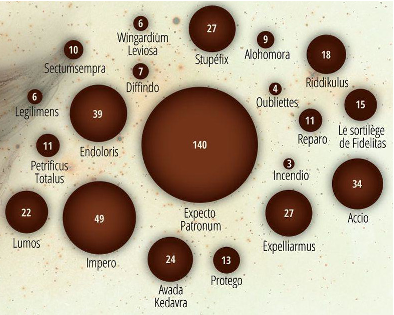
\includegraphics[width=7.9cm]{infographie} \par
         {\footnotesize\it Source : Harry Potter, les nombres d'or de la saga, Le Figaro 2017}
         \begin{enumerate}
            \item Comment sont représentées les données dans cette infographie ?
            \item Représenter les données dans un tableau en notant uniquement les sortilèges cités plus de 20 fois.
            \item Construire un diagramme en bâtons pour les valeurs de ce tableau.
         \end{enumerate}
      \end{exercice}

      \begin{Solution}
         \begin{enumerate}
            \item Les données sont représentées sous forme de \cor{bulles proportionnelles à l'effectif}.
            \item Tableau des effectifs : \par \smallskip
               {\small
                \Stat[Tableau,Qualitatif,CouleurTab=gray!40,Largeur=5mm,Donnee=Sort,Effectif=Eff,Stretch=1.3]{E.P/140,Imp/49,End/39,Acc/34,Stup/27,Exp/27,A.K/24,Lum/22}}
            \item Diagramme en bâtons : \par
               \Stat[Graphique,Qualitatif,Grille,LectureFine,Donnée=Sort,Unitex=0.7,Unitey=0.04,Pasy=10,AngleRotationAbscisse=60,EpaisseurBatons=6,CouleurDefaut=RoyalBlue]{Expecto patronum/140,Impero/49,Endoloris/39,Accio/34,Stupéfix/27,Expelliarmus/27,Avada Kedavra/24,Lumos/22}
         \end{enumerate}
      \end{Solution}
      

      \begin{exercice} %3
         Quatre-vingts archers d'un club de tir à l'arc A ont participé à un championnat. Le nombre de points obtenus par chaque archer du club est donné par le diagramme ci-dessous. \par \medskip
         {\footnotesize      
          \Stat[Graphique,Grille,Unitex=0.62,Unitey=0.2,Pasx=1,Pasy=2,EpaisseurBatons=5,Donnee=points,Effectif=Nombre d'archers,LectureFine,Tiret,CouleurDefaut=Gray]{0/0,1/0,2/5,3/9,5/8,6/12,7/14,8/6,9/8,10/18}}
         \vspace*{-5mm}
         \begin{enumerate}
            \item 
               \begin{enumerate}
                  \item Combien d'archers ont gagné exactement six points lors de ce championnat ?
                  \item Combien d'archers ont gagné trois points ou plus lors de ce championnat ?
               \end{enumerate}
            \item Le club de tir à l'arc B a aussi participé à ce championnat. Voici quelques données :
               \begin{itemize}
                  \item Le score moyen des archers lors du championnat est 7 points.
                  \item Le score moyen des dix meilleurs archers lors du championnat est 9,9 points.
               \end{itemize}
               \begin{enumerate}
                  \item Comparer les résultats des deux clubs selon leurs scores moyens.
                  \item Comparer les résultats des deux clubs selon les scores de leurs dix meilleurs archers.
               \end{enumerate}
         \end{enumerate}
      \end{exercice}

      \begin{Solution}
         \begin{enumerate}
            \item
               \begin{enumerate}
                  \item \cor{12 d'archers} ont gagné six points.
                  \item 5 archers ont obtenu 2 points. Or, $80-5 =75$ \par
                     donc, \cor{75 ont gagné trois points ou plus}.
               \end{enumerate}
            \item 
               \begin{enumerate}
                  \item Score moyen des archers du club A : \par
                     $\overline{m} =(5\times2+9\times3+8\times5+12\times6+14\times7$ \par
                     $+6\times8+8\times9+18\times10)\div80$ \par
                     $\overline{m} =547\div80 =6,8375$. \par
                     Or, le score moyen du club B est de 7 points donc, c'est \cor{le club B} qui a le score moyen le plus élevé.
                  \item Les 10 meilleurs archers du club A ont marqué 10 points alors que la moyenne des 10 meilleurs archers du club B est de 9,9 points donc, c'est \cor{le club A} qui possède les dix meilleurs résultats.
               \end{enumerate}
         \end{enumerate}
      \end{Solution}
          
      
      \begin{exercice}[Dur] %4
         Le tableau suivant résume les résultats obtenus par une classe lors d'une évaluation. \par \medskip
            {\small 
             \Stat[Tableau,CouleurTab=gray!40,Largeur=1.5mm,Donnee=N,Effectif=E,Stretch=1.2]{3/1,5/2,6/1,7/3,8/3,9/5,10/6,11/4,12/2,13/1,14/2,17/2,18/1}}
         \begin{enumerate}
            \item Combien y a-t-il d'élèves dans cette classe ?
            \item Compléter le tableau par les fréquences.
            \item Quel est le pourcentage d'élèves ayant obtenu une note inférieure ou égale à 8 ?
            \item Déterminer la moyenne de la série de notes.
            \item Cette évaluation était la quatrième de la période. \par
               Toutes les évaluations ont le même coefficient et jusqu'alors Bastien avait 9 de moyenne ; après ce devoir, il a 9,5 de moyenne. Quelle note a-t-il obtenue à ce devoir ? 
         \end{enumerate}
      \end{exercice}

      \begin{Solution}
         \begin{enumerate}
            \item $1+2+1+3+3+5+6+4+2+1+2+2+1 =33$. \par
               Donc, \cor{il y a 33 élèves dans cette classe}.
            \item Tableau des fréquences en \%. \par \smallskip
               \hspace*{-5mm}
               {\small
                \Stat[Tableau,CouleurTab=gray!40,Largeur=1mm,Donnee=Note,Effectif=Effectif,Stretch=1.3,Frequence]{3/1,5/2,6/1,7/3,8/3,9/5,10/6,11/4,12/2,13/1,14/2,17/2,18/1}} \smallskip
            \item $p =\dfrac{1+2+1+3+3}{33}\times100 =\dfrac{10}{33}\times100 \approx30,3$. \par \smallskip
               Environ \cor{30,3\,\% des élèves} ont obtenu une note inférieure ou égale à 8.
            \item $\overline{m} =(1\times3+2\times5+1\times6+3\times7+3\times8+5\times9+6\times10+4\times11$ \par
               $+2\times12+1\times13+2\times14+2\times17+1\times18)\div33$ \par
               $\overline{m} =330\div33 =10$. \par
               \cor{La moyenne est de 10}.
            \item La moyenne après le 4\up{e} devoir est de 9,5 donc, la somme de ses notes est de $4\times9,5 =38$. \par
               Or, la somme des trois premiers devoirs était de $3\times9 =27$.  On a, $38-27 =11$ donc  : \par
               \cor{Bastien a obtenu 11} au dernier devoir.
         \end{enumerate}
      \end{Solution}

   \end{multicols}

\end{Maquette}


%%% Récré %%%
\begin{Maquette}[Cours]{Theme={Activité récréative},Couleur={IndianRed}}
    
   \ARtitre{Cryptographie}

      La cryptographie est l'ensemble des techniques permettant de protéger une communication au moyen d'un code graphique secret. Parmi elles, on retrouve la méthode de substitution monoalphabétique : les lettres du texte à coder sont remplacées par d’autres lettres tel que  deux lettres différentes sont codées de façons différentes et que la même lettre est toujours codée de la même façon. \par
      \begin{minipage}{12cm}
         Le savant arabe {\it Al-Kindi}  (Abu Yūsuf Ya'qūb ibn'Ishāq as-Sabbāh al-Kindī) met au point, au 9\up{e} siècle, une technique appelée analyse des fréquences afin de déchiffrer les messages secrets. Elle repose sur la comparaison entre les fréquences d'apparition des lettres dans un message crypté à partir d'une langue connue avec la fréquence d'apparition moyenne des lettres dans cette langue. \par
         En français, par exemple, on a la répartition suivante représentée par \par
         un diagramme en bâtons, basée sur l'analyse de milliers de romans. 
      \end{minipage}
      \hfill
      \begin{minipage}{4cm}
         
\includegraphics[width=3.5cm]{Al-kindi}
      \end{minipage}
      \begin{center}
         {\footnotesize
          \Stat[Graphique,Qualitatif,Donnee={},Effectif=Fréquence d'apparition de la lettre (\%),Grille,Unitex=0.6,Unitey=0.35,EpaisseurBatons=4,LectureFine,Tiret,CouleurDefaut=Gray]{A/7.68,B/0.8,C/3.32,D/3.6,E/17.76,F/1.06,G/1.1,H/0.64,I/7.23,J/0.19,K/0,L/5.89,M/2.72,N/7.61,O/5.34,P/3.24,Q/1.34,R/6.81,S/8.23,T/7.3,U/6.05,V/1.27,W/0,X/0.54,Y/0.21,Z/0.07}}
      \end{center}  
      Ainsi, il y a des chances que la lettre la plus fréquente du message crypté soit la traduction de la lettre E, très fréquente en français. Les lettres très peu fréquentes ou absentes dans un message auront tendance à être les traductions de K ou W, par exemple. \par \bigskip

      Calculer la fréquence de chaque lettre du message codé ci-dessous (on pourra représenter les résultats dans un tableau). En observant les correspondances entre le diagramme en bâton et votre tableau, décoder le message. 
      \begin{center}
         \tcbset{width=14cm,colback=Gold!50}
         \begin{tcolorbox}
            BKSMAMZCZMTFY \; KF \; OKATOCFZ \; ZHKY \; CYZIAMKIYKUKFZ \; AK \; UKYYCLK \par
            ATOK \; RTIY \; CRKP \; BHCFADM \; IF \; XCY \; OKAMYMB \; RKHY \; SC \; YTSIZMTF \par
            BMFCSK \; OCFY \; AKZZK \; CAZMRMZK \; UCZDKUCZMGIK \; VHCRT
         \end{tcolorbox}
      \end{center}

      \vfill
      
      {\it Pour retrouver la correspondance de chaque lettre, on pourra tout d'abord retrouver la lettre la plus fréquente qui correspond à un E, puis chercher les mots courts de 2 lettres par exemple.
      
      \vfill
      
      \hspace*{9.5cm}\rotatedown{Spoiler : l'un des mots du message décrypté est \og message \fg.}}

\end{Maquette}
    \pagebreak
    \themeN
\chapter{Multiples et diviseurs}
\label{S07}

\programme%
   {\item Multiples et diviseurs.
    \item Critères de divisibilité par 2, 3, 5, 9.
    \item Division euclidienne.}
   {\item Déterminer si un entier est ou n'est pas multiple ou diviseur d'un autre entier.
    \item Utiliser un critère de divisibilité par 2, 3, 5, 9, 10.
    \item Modéliser et résoudre des problèmes mettant en jeu la divisibilité.}

\vfill

\begin{debat}{Débat : la division euclidienne}
   Le nom de {\bf division euclidienne} est un hommage rendu à {\it Euclide} (300 av. J.-C.), mathématicien grec qui en explique le principe par soustractions successives dans son \oe uvre {\it Les éléments}. Mais elle apparaît très tôt dans l'histoire des mathématiques, par exemple dans les mathématiques égyptiennes, babyloniennes et chinoises.
   \tcblower
      \begin{pspicture}(0,1.25)(4,4.25)
         \psline[linewidth=1mm](2,1)(2,4)
         \psline[linewidth=1mm](2,3)(4,3)
         \it\large
         \rput(0.8,3.5){dividende}
         \rput(3,3.5){diviseur}
         \rput(3,2.5){quotient}
         \rput(3,2){\small (euclidien)}
         \rput(1,1.5){reste}
      \end{pspicture}
\end{debat}

\hfill {\gray Vidéo : \href{https://www.youtube.com/watch?v=e-noKy-HD0Y&embeds_referring_euri=https%3A%2F%2Fwww.arieka.fr%2F&source_ve_path=Mjg2NjY&feature=emb_logo}{\bf Critères de divisibilité}, chaîne YouTube {\it Rapémathiques} d'{\it A'Rieka}.}


%%% Approche %%%
\begin{Maquette}[Cours]{Theme={Activité d'approche},Couleur={SteelBlue}}

   \AAtitre{Les multiplications incomplètes}

      {\it Objectifs : calculer mentalement des multiplications et des divisions ; résoudre un problème de calcul mental ; compléter un tableau à double entrée.}

      \begin{AActivite}

         Compléter ces tables de multiplication dont on a effacé le contenu de certaines cases. Les nombres sont tous strictement positifs, il ne peut pas y avoir deux fois le même nombre sur une même colonne ou une même ligne. \par
         
         {\hautab{1.5}
         \AApartie{Piste verte} \medskip
            \hskip10mm
            \begin{tabular}{|C{0.5}||C{0.5}|C{0.5}|}
               \hline
               {\Large $\times$} & & \\
               \hline\hline
               & & 24 \\
               \hline
               & 25 & 30 \\
               \hline
            \end{tabular}
            \hskip10mm
            \begin{tabular}{|C{0.5}||C{0.5}|C{0.5}|}
               \hline
               {\Large $\times$} & & 7 \\
               \hline\hline
               & & 21 \\
               \hline
               4 & 8 & \\
               \hline
            \end{tabular}
            \hskip10mm
            \begin{tabular}{|C{0.5}||C{0.5}|C{0.5}|}
               \hline
               {\Large $\times$} & 6 & \\
               \hline\hline
               & 24 & 32 \\
               \hline
               & 36 & \\
               \hline
            \end{tabular}
            \hskip10mm
            \begin{tabular}{|C{0.5}||C{0.5}|C{0.5}|}
               \hline
               {\Large $\times$} & 3 & \\
               \hline\hline
               & & 18 \\
               \hline
               5 & & 45 \\
               \hline
            \end{tabular}
               
         \bigskip
         \AApartie{Piste bleue} \medskip
            \hskip10mm
            \begin{tabular}{|C{0.5}||C{0.5}|C{0.5}|C{0.5}|}
               \hline
               {\Large $\times$} & 2 & & \\
               \hline\hline
               & & 9 & \\
               \hline
               & 8 & & \\
               \hline
               & 16 & & 56 \\
               \hline
            \end{tabular}
            \hskip16mm
            \begin{tabular}{|C{0.5}||C{0.5}|C{0.5}|C{0.5}|}
               \hline
               {\Large $\times$} & 2 & & \\
               \hline\hline
               4 & & 16 & \\
               \hline
               & & & 35 \\
               \hline
               & 18 & & 45 \\
               \hline
            \end{tabular}
            \hskip16mm
            \begin{tabular}{|C{0.5}||C{0.5}|C{0.5}|C{0.5}|}
               \hline
               {\Large $\times$} & & 7 & \\
               \hline\hline
               & 12 & & 32 \\
               \hline
               & & & 64 \\
               \hline
               & & 63 & 72 \\
               \hline
            \end{tabular}
      
      \bigskip
      \AApartie{Piste rouge} \medskip
         \hskip10mm
         \begin{tabular}{|C{0.5}||C{0.5}|C{0.5}|C{0.5}|}
            \hline
            {\Large $\times$} & & 3 & \\
            \hline\hline
            & 21 & & \\
            \hline
            & & 18 & \\
            \hline
            & & 6 & 4 \\
            \hline
         \end{tabular}
         \hskip16mm
         \begin{tabular}{|C{0.5}||C{0.5}|C{0.5}|C{0.5}|}
            \hline
            {\Large $\times$} & & & 7 \\
            \hline\hline
            2 & & & \\
            \hline
            & 72 & 54 & \\
            \hline
            & 40 & & 35 \\
            \hline
         \end{tabular}
         \hskip16mm
         \begin{tabular}{|C{0.5}||C{0.5}|C{0.5}|C{0.5}|}
            \hline
            {\Large $\times$} & & & \\
            \hline\hline
            & 18 & & 15 \\
            \hline
            & & 64 & \\
            \hline
            & & 32 & \\
            \hline
         \end{tabular}
         
      \bigskip
      \AApartie{Piste noire} \medskip
         \hskip10mm
         \begin{tabular}{|C{0.5}||C{0.5}|C{0.5}|C{0.5}|}
            \hline
            {\Large $\times$} & & & 10 \\
            \hline\hline
            & 20 & 8 & \\
            \hline
            & 35 & & 70 \\
            \hline
            & & & 100 \\
            \hline
         \end{tabular}
         \hskip16mm
         \begin{tabular}{|C{0.5}||C{0.5}|C{0.5}|C{0.5}|}
            \hline
            {\Large $\times$} & & & \\
            \hline\hline
            & & 45 & \\
            \hline
            & 28 & & \\
            \hline
            & 44 & & 99 \\
            \hline
         \end{tabular}
         \hskip16mm
         \begin{tabular}{|C{0.5}||C{0.5}|C{0.5}|C{0.5}|}
            \hline
            {\Large $\times$} & & 13 & \\
            \hline\hline
            & & 65 & \\
            \hline
            & 42 & & 49 \\
            \hline
            & 72 & & 84 \\
            \hline
         \end{tabular}}

      \end{AActivite}

\end{Maquette}


%%% Trace écrite %%%
\begin{Maquette}[Cours]{Theme={Trace écrite},Couleur={0.4[SteelBlue,Black]}}

   %%% 1
   \section{Multiples et diviseurs}

      \begin{minipage}{10cm}
         {\it Rappel :} effectuer une division euclidienne d'un {\bf dividende} $a$ par un {\bf diviseur} $b$, c'est trouver deux entiers appelés {\bf quotient} $q$ et {\bf reste} $r$ tels que $a=b\times q+r$ où $r<b$. \par
         Dans l'exemple ci-contre, on peut écrire : $123 =5\times24+3$.
      \end{minipage}
      \qquad
      \begin{minipage}{5cm}
         \begin{pspicture}(-0.5,-1)(4,4)
            \rput(1,1.2){$\opidiv[displayintermediary=all,voperation=top]{123}{5}$}
            \psline[linecolor=DodgerBlue]{->}(0.7,2.8)(0.7,2.4)
            \rput(0.7,3){\textcolor{DodgerBlue}{dividende}}
            \psline[linecolor=DodgerBlue]{<-}(1.9,2.3)(2.4,2.3)
            \rput[l](2.5,2.3){\textcolor{DodgerBlue}{diviseur}}
            \psline[linecolor=Crimson]{<-}(2.2,1.7)(2.7,1.7)
            \rput[l](2.8,1.7){\textcolor{Crimson}{quotient}}
            \psline[linecolor=Crimson]{<-}(1.4,0.2)(1.9,0.2)
            \rput[l](2,0.2){\textcolor{Crimson}{reste}}
         \end{pspicture}
      \end{minipage}

      \begin{definition*}{}
         $a$ et $b$ sont deux nombres entiers. Lorsque le reste de la division de $a$ par $b$ est égal à 0, on dit que $a$ est un \textbf{multiple} de $b$, ou que $b$ est un \textbf{diviseur} de $a$, ou que $a$ est \textbf{divisible} par $b$.
      \end{definition*}

      \begin{exemple*}{}
         \begin{itemize}
            \item 15 est multiple de 3 car $15=3\times 5+\textcolor{DodgerBlue}{0}$, on peut aussi dire que 3 est un diviseur de 15, ou que 15 est divisible par 3.
            \item 17 n'est pas un multiple de 3 car $17=3\times 5+\textcolor{DodgerBlue}{2}$.
            \item Les diviseurs de 24 sont 1; 2; 3; 4; 6; 8; 12 et 24.
            \item Il y a une infinité de multiples de 18, comme par exemple 18 ; 36 ; 54 ; 180\dots
         \end{itemize}
      \end{exemple*}

   %%% 2
   \section{Critères de divisibilité}
   
   \begin{propriete*}{}
      \begin{itemize}
         \item un nombre est divisible par 2 s'il se termine par 0 ; 2 ; 4 ; 6 ou 8 ;
         \item un nombre est divisible par 5 s'il se termine par 0 ou 5 ;
         \item un nombre est divisible par 10 s'il se termine par 0 ;
         \item un nombre est divisible par 3 si la somme de ses chiffres est un multiple de 3 ;
         \item un nombre est divisible par 9 si la somme de ses chiffres est un multiple de 9.
      \end{itemize}
   \end{propriete*}
   
   \begin{exemple*}{}   
      \begin{itemize}
         \item $2+5+2=9$ est multiple de 3 donc, 252 est divisible par 3. \par
            $2+5+3=10$ n'est pas multiple de 3 donc, 253 n'est pas divisible par 3.
         \item $5+2+3+6+2=18$ est multiple de 9 donc, 52\,362 est divisible par 9, et donc par 3. \par
            $5+2+3+6+3=19$ n'est pas multiple de 9 donc, 52\,363 n'est pas divisible par 9.
         \end{itemize}
   \end{exemple*}
   
   Remarque : pour savoir si un nombre est divisible par 3, on peut calculer la somme des chiffres du nombre obtenu jusqu'à ce que l'on trouve un seul chiffre. \par
      pour \num{563387981}, on calcule : $5+6+3+3+8+7+9+8+1=50$. \par
      Puis on calcule $5+0=5$. 5 n'est pas divisible par 3 donc, \num{563387981} n'est pas divisible par 3.

\end{Maquette}


%% Exercices %%%%%%%
\begin{Maquette}[Fiche,CorrigeFin,Colonnes=2]{}

   \begin{multicols}{2}

      \begin{exercice} %1
         Effectuer les divisions euclidiennes suivantes : \par
         307 par 7 \qquad et \qquad \num{13758} par 25.
      \end{exercice} 

      \begin{Solution}
         \opidiv[displayintermediary=all,voperation=top]{307}{7} \hskip1.5cm \opidiv[displayintermediary=all,voperation=top]{13758}{25} \par \smallskip
         \cor{$307 =7\times43+6$} \quad et \quad \cor{$13\,758 =25\times550+8$}.
       \end{Solution}
      

      \begin{exercice} %2
         Résoudre les problèmes suivants :
         \begin{enumerate}
            \item \num{6798} supporters d'un club de rugby doivent faire un déplacement en car pour soutenir leur équipe. Chaque car dispose de 55 places. \par
               Combien de cars faut-il réserver ?
            \item Des stylos sont conditionnés par boîte de 40. Imane a \num{2647} stylos. \par
               Combien lui en manque-t-il pour avoir des boîtes entièrement remplies ?
            \item Trois amis participent à une chasse au trésor et trouvent \num{1419} pièces en chocolat. \par
               Si le partage est équitable, combien de pièces en chocolat auront-ils chacun ? \par
               Julie arrive et leur rappelle que c'est elle qui leur a prêté sa boussole. Elle exige donc d'avoir la même part que chacun des trois autres plus les pièces restantes. Combien de pièces recevra-t-elle ?
         \end{enumerate}
      \end{exercice}

      \begin{Solution}
         On effectue les divisions suivantes : \par 
         {\small \opidiv[displayintermediary=all,voperation=top]{6798}{55} \hfill \opidiv[displayintermediary=all,voperation=top]{2647}{40} \hfill \opidiv[displayintermediary=all,voperation=top]{1419}{3}}
         \begin{enumerate}
            \item En prenant 123 cars, il restera 33 personnes, il faudra donc réserver \cor{124 cars}.
            \item Il lui reste 7 stylos pour une boite de 40, il faut donc ajouter \cor{33 stylos} pour compléter la boite.
            \item Chaque ami aura donc \cor{473 pièces en chocolat}, il n'en restera pas. Lorsque Julie arrive, elle recevra $(354+3)$ pièces en chocolat, soit \cor{357}.
         \end{enumerate}
      \end{Solution}
      
  
      \begin{exercice} %3
         Trouver tous les diviseurs des nombres suivants :
         \begin{colenumerate}
            \item 14
            \item 40
            \item 48
            \item \num{2037}
         \end{colenumerate}
      \end{exercice}

      \begin{Solution}
         \begin{enumerate}
            \item Diviseurs de 14 : \cor{1 ; 2 ; 7 ; 14}.
            \item Diviseurs de 40 : \cor{1 ; 2 ; 4 ; 5 ; 8 ; 10 ; 20 ; 40}.
            \item Diviseurs de 48 : \cor{1 ; 2 ; 3 ; 4 ; 6 ; 8 ; 12 ; 16 ; 24 ; 48}.
            \item Diviseurs de 2\,037 : \cor{1 ; 3 ; 7 ; 21 ; 97 ; 291 ; 679 ; 2037}.
         \end{enumerate}
      \end{Solution}
      
      
      \begin{exercice} %4
         Écrire :
         \begin{enumerate}
            \item La liste des dix premiers multiples de 6.
            \item Cinq multiples de 11.
            \item Tous les multiples de 13 inférieurs à 80.
            \item Le plus grand multiple de 12 inférieur à 75.
            \item Le plus grand multiple de 36 inférieur à 100.
            \item Le plus petit multiple de 9 supérieur à \num{1200}.
            \item Le plus petit multiple de 14 supérieur à 710 ?
            \item Le plus petit et le plus grand diviseur de 199.
         \end{enumerate}
      \end{exercice}

      \begin{Solution}
         \begin{enumerate}
            \item Dix premiers multiples de 6 : \par
               \cor{0 ; 6 ; 12 ; 18 ; 24 ; 30 ; 36 ; 42 ; 48 ; 54}.
            \item Cinq multiples de 11 : \cor{0 ; 11 ; 22 ; 33 ; 44}.
            \item Multiples de 13 inférieurs à 80 : \cor{0 ; 13 ; 26 ; 39 ; 52 ; 65 ; 78}
            \item Plus grand multiple de 12 inférieur à 75 : \cor{72}.
            \item Plus grand multiple de 36 inférieur à 100 : \cor{72}.
            \item Plus petit multiple de 9 supérieur à 1\,200 : \cor{\num{1206}}.
            \item Plus petit multiple de 14 supérieur à 710 : \cor{714}.
            \item Plus grand/petit diviseur de 199 : \cor{1 et 199}.
         \end{enumerate}
      \end{Solution}
      
      
      \begin{exercice}[Dur] %5
         Je suis un nombre impair à deux chiffres sans 2 dans mon écriture. Je ne suis pas divisible par 5 mais je suis un multiple de 9. \par
         Qui suis-je ? 
      \end{exercice}

      \begin{Solution}
         \begin{itemize}
            \item On peut commencer par écrire la liste des multiples de 9 à deux chiffres : 18 ; 27 ; 36 ; 45 ; 54 ; 63 ; 72 ; 81 ; 90 ; 99.
            \item On supprime ensuite les nombres pairs, il reste : \par
               27 ; 45 ; 63 ; 81 ; 99.
            \item On supprime 27 qui comporte un 2, il reste : 45 ; 63 ; 81 ; 99.
            \item Enfin, on supprime 45 qui est divisible par 5. \par
               Je peux donc être \cor{63, 81 ou 99}.
         \end{itemize}
      \end{Solution}
      
      
      \begin{exercice} %6
         Les nombres 30 ; 27 ; 246 ; 325 ; \num{4238} et \num{6139} sont-ils divisibles par 2 ? par 3 ? par 5 ? par 9 ?
      \end{exercice}
      \begin{Solution}
         On résume les résultats dans un tableau : \par \smallskip
         {\hautab{1}
         \begin{tabular}{|*{7}{c|}}
            \hline
            & 30 & 27 & 246 & 325 & \num{4238} & \num{6139} \\
            \hline
            par 2 & \textcolor{RoyalBlue}{$\times$} & & \textcolor{RoyalBlue}{$\times$} & & \textcolor{RoyalBlue}{$\times$} & \\
            \hline
            par 3 & \textcolor{RoyalBlue}{$\times$} & \textcolor{RoyalBlue}{$\times$} & \textcolor{RoyalBlue}{$\times$} & & & \\
            \hline
            par 5 & \textcolor{RoyalBlue}{$\times$} & & & \textcolor{RoyalBlue}{$\times$} & & \\
            \hline
            par 9 & & \textcolor{RoyalBlue}{$\times$} & & & & \\
            \hline
         \end{tabular}}
      \end{Solution}
      
      
      \begin{exercice} %7
         Relier les deux cases grisées en suivant un chemin constitué uniquement de multiples de 6. \par \smallskip
         \LabyNombre[Nom=Ex7,Graine=1,Multiple=6,Couleur=LightGrey,Echelle=1.1]
      \end{exercice}

      \begin{Solution}
         \smallskip
         \LabyNombre[Nom=Ex7,Graine=1,Multiple=6,Couleur=LightGrey,Echelle=1,Solution,CouleurChemin=1.5RoyalBlue]
      \end{Solution}
      
      
      \begin{exercice} %8
         Colorier un chemin qui permet de relier les deux cases grisées en suivant les lignes sachant que le nombre inscrit dans un carré vers lequel on se déplace doit être multiple du nombre inscrit dans le disque d’où l’on vient et que le nombre inscrit dans un disque vers lequel on se déplace doit être diviseur du nombre inscrit dans le carré d’où l’on vient. \par \medskip
         \LabyNombre[Nom=Ex8,Graine=2,Multiplication,Multiple=6,Longueur=7,Largeur=5,Couleur=LightGrey,Echelle=0.6]
      \end{exercice}

      \begin{Solution}
         \medskip
         \LabyNombre[Nom=Ex8,Graine=2,Multiplication,Multiple=6,Longueur=7,Largeur=5,Couleur=LightGrey,Echelle=0.6,Solution]
      \end{Solution}
   
      
      \begin{exercice}[Dur] %9
         Répondre par vrai ou faux en justifiant.
         \begin{enumerate}
            \item Tout nombre divisible par 3 est divisible par 9.
            \item Tout nombre divisible par 9 est divisible par 3.
            \item Tout nombre divisible par 2 et 3 est divisible par 5.
            \item Tout nombre dont le chiffre des unités est 2 est divisible par 2. 
            \item Tout nombre dont le chiffre des unités est 3 est divisible par 3.
         \end{enumerate}
      \end{exercice}

      \begin{Solution}
         \begin{enumerate}
            \item \cor{faux}. Par exemple, 6 est divisible par 3 mais pas par 9.
            \item \cor{vrai}. Un nombre divisible par 9 s'écrit $9k$ où $k$ est un entier. Or, $9k =3\times(3k)$ donc il est divisible par 3.
            \item \cor{faux}. Par exemple, 6 est divisible par 2 et par 3 mais il n'est pas divisible par 5.
            \item \cor{vrai}. Un nombre pair est divisible par 2.
            \item \cor{faux}. Par exemple, 13 se termine par 3 mais n'est pas divisible par 3.
         \end{enumerate}
      \end{Solution}

   \end{multicols}

\end{Maquette}


%%% Récré %%%
\begin{Maquette}[Cours]{Theme={Activité récréative},Couleur={IndianRed}}
    
   \ARtitre{Shikaku}
      Le {\bf Shikaku} est un casse-tête japonais. Son nom vient du Japonais et signifie \og diviser en carrés \fg. \\
      Le but de ce jeu est de diviser une grille donnée en plusieurs rectangles. \medskip
         
      \ARpartie{Règle du jeu}
         \begin{itemize}
            \item Paver la grille à l'aide de rectangles.
            \item Chaque rectangle doit contenir un nombre et un seul.
            \item Le nombre contenu dans un rectangle indique combien de cases le constituent. \medskip
         \end{itemize}
   
      \ARpartie{Exemple}
         {\psset{unit=0.6,subgriddiv=0,gridlabels=0,gridwidth=0.15mm}
          \footnotesize
            \begin{tabular}{*{6}{C{2.5}}}
               \begin{pspicture}(0,0)(4,4)
                  \psgrid(0,0)(4,4)
                  \rput(3.5,3.5){4}
                  \rput(2.5,2.5){6} \rput(3.5,2.5){3} 
                  \rput(0.5,0.5){2} \rput(2.5,0.5){1}           
               \end{pspicture}
               &
               \begin{pspicture}(0,0)(4,4)
                  \psgrid(0,0)(4,4)
                  \rput(3.5,3.5){4}
                  \rput(2.5,2.5){6} \rput(3.5,2.5){3} 
                  \rput(0.5,0.5){2} \rput(2.5,0.5){1} 
                 \psset{linewidth=0.6mm,linecolor=RoyalBlue}
                  \psframe(2,0)(3,1)
               \end{pspicture}
               &
               \begin{pspicture}(0,0)(4,4)
                  \psgrid(0,0)(4,4)
                  \rput(3.5,3.5){4}
                  \rput(2.5,2.5){6} \rput(3.5,2.5){3} 
                  \rput(0.5,0.5){2} \rput(2.5,0.5){1} 
                  \psset{linewidth=0.6mm,linecolor=RoyalBlue}
                  \psframe(2,0)(3,1)
                  \psframe(0,3)(4,4)
               \end{pspicture}
               &
               \begin{pspicture}(0,0)(4,4)
                  \psgrid(0,0)(4,4)
                  \rput(3.5,3.5){4}
                  \rput(2.5,2.5){6} \rput(3.5,2.5){3} 
                  \rput(0.5,0.5){2} \rput(2.5,0.5){1} 
                  \psset{linewidth=0.6mm,linecolor=RoyalBlue}
                  \psframe(2,0)(3,1)
                  \psframe(0,3)(4,4)
                  \psframe(3,0)(4,3)
               \end{pspicture}
               &
               \begin{pspicture}(0,0)(4,4)
                  \psgrid(0,0)(4,4)
                  \rput(3.5,3.5){4}
                  \rput(2.5,2.5){6} \rput(3.5,2.5){3} 
                  \rput(0.5,0.5){2} \rput(2.5,0.5){1} 
                  \psset{linewidth=0.6mm,linecolor=RoyalBlue}
                  \psframe(2,0)(3,1)
                  \psframe(0,3)(4,4)
                  \psframe(3,0)(4,3)
                  \psframe(0,1)(3,3)
               \end{pspicture}
               &
               \begin{pspicture}(0,0)(4,4)
                  \psgrid(0,0)(4,4)
                  \rput(3.5,3.5){4}
                  \rput(2.5,2.5){6} \rput(3.5,2.5){3} 
                  \rput(0.5,0.5){2} \rput(2.5,0.5){1} 
                  \psset{linewidth=0.6mm,linecolor=RoyalBlue}
                  \psframe(2,0)(3,1)
                  \psframe(0,3)(4,4)
                  \psframe(3,0)(4,3)
                  \psframe(0,1)(3,3)
                  \psframe(0,0)(2,1)
               \end{pspicture}
               \\
               grille d'origine
               &
               un rectangle à 1 case est forcément un carré de côté 1
               &
               un rectangle à 4 cases est un carré de côté 2 ou un rectangle de côtés 1 et 4
               &
               un rectangle à 3 cases est un rectangle de côtés 1 et 3
               &
               un rectangle à 6 cases est un rectangle de côtés 2 et 3 ou de côtés 1 et 6
               &
               un rectangle à 2 cases est un rectangle de côtés 1 et 2 \\
            \end{tabular}} \smallskip
   
      \ARpartie{Let's go !!!}
         \Shikaku[Taille=4,Largeur=5mm,Couleur=RoyalBlue]{%
            /2,l/2,l/4,/,%1
            b/,lb/,lb/,b/,%2
            /2,lb/3,b/,b/,%3
            /,l/,/,/3}%4
         \hskip1cm
         \Shikaku[Taille=5,Largeur=5mm,Couleur=RoyalBlue,Sotion]{%
            /3,lb/,b/,b/4,b/,%1
            /,lb/,b/2,l/,/,%2
            b/,l/,l/,lb/4,b/,%3
            /,lb/2,lb/2,lb/2,b/,%4
            /2,l/,/4,/,/}%5
         \hskip1cm
         \Shikaku[Taille=6,Largeur=5mm,Couleur=RoyalBlue]{%
            /4,l/5,l/,lb/,b/3,b/,%1
            /,l/,l/3,l/,/,/,%2
            /,l/,lb/,lb/6,b/,b/,%3
            b/,l/,lb/,b/,b/4,b/,%4
            /,lb/,lb/,b/2,lb/2,b/,%5
            /2,l/,/5,/,/,/}%6

         \vskip5mm

         \Shikaku[Taille=7,Largeur=5mm,Couleur=RoyalBlue]{%
            /,l/,/,/,l/,lb/,b/2,%1
            /,lb/,b/,b/6,lb/2,l/2,l/2,%2
            /,lb/2,b/,l/4,/,lb/,lb/,%3
            /6,l/,l/3,lb/,b/,l/,/,%4
            /,l/3,l/,l/,/,lb/4,b/,%5
            b/,lb/,lb/,lb/4,b/,l/2,l/2,%6
            /,/2,l/,/,/3,l/,l/}%7
         \hskip1cm
         \Shikaku[Taille=9,Largeur=5mm,Couleur=RoyalBlue]{%
            b/2,b/,l/,/,/,l/,l/,l/,/,%1
            /2,l/,lb/6,b/,b/,l/3,lb/2,lb/4,b/,%2
            b/,l/,l/,lb/2,b/,lb/,l/,lb/2,b/,%3
            /,l/,l/,l/2,lb/,b/2,l/,l/,/,%4
            /5,l/,l/6,lb/,lb/,b/2,lb/3,lb/4,b/,%5
            /,l/7,l/,l/3,l/,/,/,l/,/,%6
            /,l/,l/,l/,l/,/,/,l/6,/,%7
            b/,lb/,lb/,lb/,lb/9,b/,b/,lb/,b/,%8
            /,/3,/,l/,/4,/,/,l/2,/}%9

\end{Maquette}
    \pagebreak
    \graphicspath{{../../S08_Somme_des_angles_d_un_triangle/Images/}}

\themeG
\chapter{Somme des angles d'un triangle}
\label{S08}

\programme%
   {\item Somme des angles d'un triangle.}
   {\item Mener des raisonnements et s'initier à la démonstration en utilisant les propriétés d'une figure.}

\vfill

\begin{debat}{Débat : géométrie euclidienne VS géométrie sphérique}
   \og Un ours part de sa caverne et parcourt \Lg[km]{10} vers le sud, puis \Lg[km]{10} vers l'est et enfin \Lg[km]{10} vers le nord. Il se retrouve alors juste devant l'entrée de sa caverne. Quelle est la couleur de l'ours ? \fg \par
   La {\bf géométrie sphérique} n'a pas les même propriétés que la {\bf géométrie euclidienne} utilisée au collège et au lycée. Cette dernière est la géométrie initiée par {\it Euclide}, mathématicien grec né vers 330 av. J.-C., il est connu pour avoir recensé une grande partie des mathématiques de l'époque dans ses {\it Éléments} : une série de treize livres utilisée pendant près de 2\,000 ans qui fut l'ouvrage le plus édité au monde après la Bible.
   \tcblower
      \begin{minipage}{5cm}
         \begin{pspicture}(-1,-1)(4,3)
            \pspolygon[linecolor=DodgerBlue](1,0)(4,0)(3,3.25)
         \end{pspicture}
      \end{minipage}
      \begin{minipage}{5cm}
         \flushright Un triangle \og sphérique \fg{} $\Longrightarrow$ \par
         \flushleft $\Longleftarrow$ Un triangle \og plat \fg \par    
      \end{minipage}
      \begin{minipage}{5cm}
         \Reperage[Espace,Sphere,EchelleEspace=60,AnglePhi=30,CouleurG=Crimson]{70/90/A,0/90/B}
      \end{minipage} 
\end{debat}

\hfill {\gray Vidéo : \href{https://www.youtube.com/watch?v=7CZrbIkWUc4&embeds_referring_euri=https%3A%2F%2Fwww.arieka.fr%2F&source_ve_path=Mjg2NjY&feature=emb_logo}{\bf Calculer la mesure du troisième angle d'un triangle}, chaîne YouTube {\it Rapémathiques} d'{\it A'Rieka}.}


%%% Approche %%%
\begin{Maquette}[Cours]{Theme={Activité d'approche},Couleur={SteelBlue}}

   \AAtitre{Des angles mouvants}

      {\it Objectifs : faire découvrir la propriété de la somme des angles d'un triangle.}

      \begin{AActivite}

         \AApartie{Construction du triangle}

            \begin{enumerate}
               \item Sur une feuille, tracer un triangle ABC quelconque puis le découper.
               \item Colorier les trois angles de trois couleurs différentes des deux côtés du triangle (une couleur par angle). \par
                  {\psset{unit=1.2}
                  \begin{pspicture}(-2,0.2)(10,5.8)
                     \rput(8.3,4.8){$\leftarrow$ colorier des deux côtés}
                     \psline[linestyle=dashed](6,5)(6,1)(6.3,1)
                     \psframe(6,1)(6.25,1.25)
                     \pswedge[fillstyle=solid,fillcolor=Crimson,linecolor=Crimson](1,1){1}{0}{38.5}
                     \pswedge[fillstyle=solid,fillcolor=DodgerBlue,linecolor=DodgerBlue](6,5){1}{218.8}{306.8}
                     \pswedge[fillstyle=solid,fillcolor=DarkOrange,linecolor=DarkOrange](9,1){1}{127}{180}
                     \pspolygon(1,1)(9,1)(6,5)
                     \rput(0.7,1){B}
                     \rput(9.3,1){C}
                     \rput(6,5.3){A}
                     \rput(6,0.7){H}     
                  \end{pspicture}}
               \item Tracer la hauteur issue du sommet A et nommer le pied de cette hauteur H.
               \item Plier le triangle ABC de manière à placer le point A sur le point H.
               \item Plier le triangle ABC de manière à placer le point B sur le point H.
               \item Plier le triangle ABC de manière à placer le point C sur le point H.
            \end{enumerate}

         \AApartie{Observations}
            \begin{enumerate}[resume]
               \item Que forment les trois angles obtenus en H ? \par
                  \pointilles
               \item Formuler cette observation en utilisant les angles $\widehat{\text A}, \widehat{\text B}$ et $\widehat{\text C}$. \par
                  \pointilles
               \item Formuler cette observation par une phrase simple et générale sans utiliser le nom des angles. \par
                  \pointilles \par
                  \pointilles
            \end{enumerate}

      \end{AActivite}

\end{Maquette}


%%%Trace écrite %%%
\begin{Maquette}[Cours]{Theme={Trace écrite},Couleur={0.4[SteelBlue,Black]}}

   %%%1
   \section{Somme des angles dans un triangle}

      \begin{propriete*}{}
         Dans un triangle, la somme de la mesure de ses trois angles est égale à \ang{180}.
      \end{propriete*}

      Par conséquent, pour qu'un triangle soit constructible, il est nécessaire que la somme de ses angles fasse \ang{180}.
         
      \begin{center}
         {\psset{unit=1}
         \begin{pspicture}(-1,0.5)(9,5)
            \pswedge[fillstyle=solid,fillcolor=Crimson,linecolor=Crimson](1,1){1}{0}{38.5}
            \pswedge[fillstyle=solid,fillcolor=DodgerBlue,linecolor=DodgerBlue](6,5){1}{218.8}{306.8}
            \pswedge[fillstyle=solid,fillcolor=DarkOrange,linecolor=DarkOrange](9,1){1}{127}{180}
            \pspolygon(1,1)(9,1)(6,5)
            \rput(0.7,1){B}
            \rput(9.3,1){C}
            \rput(6,5.3){A} 
            \rput(5.5,2.5){$\widehat{A}+\widehat{B}+\widehat{C} =\ang{180}$}
            \pswedge[fillstyle=solid,fillcolor=Crimson,linecolor=Crimson](0,3){1}{141}{180}
            \pswedge[fillstyle=solid,fillcolor=DodgerBlue,linecolor=DodgerBlue](0,3){1}{53}{141}
            \pswedge[fillstyle=solid,fillcolor=DarkOrange,linecolor=DarkOrange](0,3){1}{0}{53}
            \rput(-0.7,3.2){\white B}
            \rput(-0.1,3.6){\white A}
            \rput(0.6,3.3){\white C}
         \end{pspicture}}
      \end{center}

      \begin{exemple*}{}
         \begin{minipage}{7cm}
            \SommeAngles[FigureSeule,Rectangle,Echelle=10mm]{CBA}{}{55} \par
            Quelle est la mesure de l'angle $\widehat{BCA}$ ?
         \end{minipage}
         \qquad
         \begin{minipage}{9cm}
            D'après le codage, l'angle $\widehat{ABC}$ est droit, donc $\widehat{ABC} =\ang{90}$.
            \SommeAngles[Perso]{CBA}{90}{55}
         \end{minipage}
      \end{exemple*}


   %%%2
   \section{Triangles particuliers}

      \begin{pspicture}(-1,-3.5)(4,2.5)
         \pstTriangle[PointSymbol=none](0,0){E}(4,0){C}(0,2){R}
         \psset{fillstyle=solid}
         \pstRightAngle[fillcolor=Crimson,linecolor=Crimson]{R}{E}{C}
         \pstMarkAngle[fillcolor=DodgerBlue,linecolor=DodgerBlue]{R}{C}{E}{}
         \pstMarkAngle[fillcolor=DarkOrange,linecolor=DarkOrange]{E}{R}{C}{}
         \rput(2,-1.5){\parbox{4cm}{\quad {\bf Triangle rectangle} \par \medskip La somme des deux angles aigus est égale à \ang{90}.}}
      \end{pspicture}
      \begin{pspicture}(-2.5,-2.5)(4,3)
         \pstTriangle[PointSymbol=none](0,1){I}(4,1){O}(2,2.5){S}
         \pstSegmentMark[SegmentSymbol=MarkHashh,MarkAngle=90]{I}{S} 
         \pstSegmentMark[SegmentSymbol=MarkHashh,MarkAngle=90]{S}{O}
         \pstLineAB{I}{O}
         \psset{linecolor=DodgerBlue,fillstyle=solid,fillcolor=DodgerBlue}
         \pstMarkAngle{S}{O}{I}{}
         \pstMarkAngle{O}{I}{S}{}
         \rput(2,-1){\parbox{6cm}{\qquad {\bf Triangle isocèle} \par \medskip Les angles de la base ont la même mesure. \par Si le triangle est isocèle et rectangle, les angles de la base mesurent \ang{45}.}}
      \end{pspicture}
      \begin{pspicture}(-2.5,-3.5)(3,3)
         \pstTriangle[PointSymbol=none](0,0){E}(3,0){I}(1.5,2.55){Q}
         \psset{SegmentSymbol=MarkHash,MarkAngle=90}
         \pstSegmentMark{E}{Q} 
         \pstSegmentMark{I}{Q}
         \pstSegmentMark{I}{E}
         \psset{linecolor=DarkOrange,fillstyle=solid,fillcolor=DarkOrange,LabelSep=.75}
         \pstMarkAngle{Q}{I}{E}{\small \ang{60}}
         \pstMarkAngle{I}{E}{Q}{\small \ang{60}}
         \pstMarkAngle{E}{Q}{I}{\small \ang{60}}
         \rput(1.5,-1.5){\parbox{3cm}{{\bf Triangle équilatéral} \par \medskip Tous les angles mesurent \ang{60}.}}
      \end{pspicture}

\end{Maquette}


%%% Exercices %%%
\begin{Maquette}[Fiche,CorrigeFin,Colonnes=2]{}

   \begin{multicols}{2}

      \begin{exercice}[SLF] %1
         Pour chaque cas, calculer la mesure de l'angle manquant dans le triangle $RIM$.
         \begin{center}
            \hautab{1.25}
            \begin{tabular}{|*{3}{C{2}|}}
               \hline
               $\widehat{RIM}$ & $\widehat{IMR}$ & $\widehat{MRI}$ \\
               \hline
               \ang{124} & \ang{18} & \\
               \hline
               \ang{71} & & \ang{29} \\
               \hline
               & \ang{98,1} & \ang{59,6} \\
               \hline
               \ang{49,5} & & \ang{113} \\
               \hline
            \end{tabular}
         \end{center}
      \end{exercice}
      
      \begin{Solution}
         Pour chaque cas, la somme doit être égale à \ang{180}. \par
         {\hautab{1.5}
         \begin{tabular}{|*{3}{C{2}|}}
            \hline
            $\widehat{RIM}$ & $\widehat{IMR}$ & $\widehat{MRI}$ \\
            \hline
            \ang{124} & \ang{18} & \textcolor{RoyalBlue}{\ang{38}} \\
            \hline
            \ang{71} & \textcolor{RoyalBlue}{\ang{80}} & \ang{29} \\
            \hline
            \textcolor{RoyalBlue}{\ang{22,3}} & \ang{98,1} & \ang{59,6} \\
            \hline
            \ang{49,5} & \textcolor{RoyalBlue}{\ang{17,5}} & \ang{113} \\
            \hline
         \end{tabular}}
      \end{Solution}
      
      
      \begin{exercice} %2
         Les figures suivantes ne sont pas en vraie grandeur. Pour chacune d'elles, indiquer si elles sont constructibles ou non en justifiant la réponse. \\
         {\psset{unit=0.85}
         \small
         \begin{pspicture}(-0.5,0)(4,3.5)
            \pstTriangle[PointSymbol=none](0,0){A}(3,0){B}(2,3){C}
            \psset{LabelSep=.8}
            \pstMarkAngle{B}{A}{C}{\ang{70}}
            \pstMarkAngle{C}{B}{A}{\ang{75}} 
            \pstMarkAngle{A}{C}{B}{\ang{40}} 
         \end{pspicture}
         \begin{pspicture}(-0.5,-0.5)(4,3.5)
            \pstTriangle[PointSymbol=none](0,2){F}(3.5,2){U}(2.2,0){O}
            \psset{LabelSep=.85}
            \pstMarkAngle{O}{F}{U}{\ang{10}}
            \pstMarkAngle{U}{O}{F}{\ang{95}} 
            \pstMarkAngle{F}{U}{O}{\ang{85}} 
         \end{pspicture} \par
         \begin{pspicture}(-1,-0.5)(4,4)
            \pstTriangle[PointSymbol=none](0,2){B}(0,0){O}(3,0){F}
            \pstMarkAngle{O}{B}{F}{\ang{57,3}}
            \pstMarkAngle[LabelSep=1.2]{B}{F}{O}{\ang{32,7}} 
            \pstRightAngle{F}{O}{B}
         \end{pspicture}
         \begin{pspicture}(-0.5,-0.5)(3.5,3.5)
            \pstTriangle[PointSymbol=none](1,0){P}(0,3){I}(3,2){C}
            \pstMarkAngle{P}{I}{C}{\ang{35,1}}
            \pstMarkAngle[LabelSep=0.9]{C}{P}{I}{\ang{72,4}}
            \psset{SegmentSymbol=MarkHashh,MarkAngle=90}
            \pstSegmentMark{P}{I}
            \pstSegmentMark{I}{C}
         \end{pspicture}}
      \end{exercice}
      
      \begin{Solution}
         \begin{itemize}
            \item Dans le triangle $BAC$ : \\
               $\ang{40}+\ang{70}+\ang{75} =\ang{185} \neq \ang{180}$. \par
               \cor{Le triangle $BAC$ n'est pas constructible}.
            \item Dans le triangle $FOU$ : \\
               $\ang{10}+\ang{95}+\ang{85} =\ang{190} \neq \ang{180}$. \par
               \cor{Le triangle $FOU$ n'est pas constructible}.
            \item Dans le triangle $BOF$ : \\
               $\ang{57,3}+\ang{32,7}+\ang{90} =\ang{180}$. \par
               \cor{Le triangle $BOF$ est constructible}.
            \item Dans le triangle $PIC$ : \\
               $\ang{35,1}+\ang{72,4}+\ang{72,4} =\ang{179,9} \neq \ang{180}$. \par
               \cor{Le triangle $PIC$ n'est pas constructible}.
         \end{itemize}
      \end{Solution}
      
      
      \begin{exercice} %3
         Calculer, pour chaque triangle, la mesure de l'angle marqué d'un point d'interrogation. \par
         {\psset{unit=0.85}
         \small
         \begin{pspicture}(-1,0)(3.5,3.7)
            \pstTriangle[PointSymbol=none](0,0){R}(3,0){E}(1.5,2.6){P}
            \psset{SegmentSymbol=MarkHash,MarkAngle=90,LabelSep=0.8}
            \pstSegmentMark{R}{E}
            \pstSegmentMark{R}{P}
            \pstSegmentMark{P}{E}
            \pstMarkAngle{P}{E}{R}{?} 
         \end{pspicture}
         \begin{pspicture}(0,-0.5)(4,3.2)
            \pstTriangle[PointSymbol=none](0,2.3){R}(4,2.3){P}(2,0.3){A}
            \psset{SegmentSymbol=MarkHashh,MarkAngle=90}
            \pstSegmentMark{R}{A}
            \pstSegmentMark{P}{A}
            \pstMarkAngle[LabelSep=0.75]{P}{A}{R}{?} 
            \pstMarkAngle[LabelSep=0.9]{A}{R}{P}{\ang{38}}
         \end{pspicture} \par  
         \begin{pspicture}(-1,-0.5)(3.5,3.3)
            \pstTriangle[PointSymbol=none](0,2){Y}(0,0){E}(3,0){S}
            \pstMarkAngle[LabelSep=1.1]{E}{Y}{S}{\small \ang{50,36}}
            \pstRightAngle{S}{E}{Y}
            \pstMarkAngle[LabelSep=0.8]{Y}{S}{E}{?}
         \end{pspicture}
         \begin{pspicture}(-1,-0.5)(3.5,3.8)
            \pstTriangle[PointSymbol=none](1,0){H}(0,3){W}(3,2){Y}
            \pstMarkAngle{H}{W}{Y}{\ang{42,6}}
            \psset{SegmentSymbol=MarkHashh,MarkAngle=90}
            \pstSegmentMark{W}{H}
            \pstSegmentMark{W}{Y}
            \pstMarkAngle[LabelSep=0.8]{Y}{H}{W}{?}
         \end{pspicture}}
      \end{exercice}
      
      \begin{Solution}
         \begin{itemize}
            \item Le triangle $REP$ est équilatéral donc, tous ses angles ont la même mesure. La somme faisant \ang{180}, un angle mesure $\ang{180}\div3 =\ang{60}$. \par
               Conclusion : \cor{$\widehat{REP} =\ang{60}$}.
            \item Le triangle $RAP$ est isocèle en $A$ dont les angles à sa base principale mesurent \ang{38}. \par
            $\ang{38}+\ang{38} =\ang{76}$ d'où $\widehat{RAP} =\ang{180}-\ang{76} =\ang{104}$. \par
            Conclusion : \cor{$\widehat{RAP} =\ang{104}$}. 
            \item Le triangle $YES$ est rectangle en $E$ et $\ang{90}+\ang{50,36} =\ang{140,36}$ d'où, $\widehat{ESY} =\ang{180}-\ang{140,36} =\ang{39,64}$. \par
               Conclusion : \cor{$\widehat{ESY} =\ang{39,64}$}. 
            \item Le triangle $WHY$ est isocèle en $W$ dont l'angle à son sommet principal vaut \ang{42,6}. \par
               $\ang{180}-\ang{42,6} =\ang{137,4}$ ; $\widehat{WHY} =\ang{137,4}\div2 =\ang{68,7}$. \par
               Conclusion : \cor{$\widehat{WHY} =\ang{68,7}$}.
         \end{itemize}
      \end{Solution}
      
      
      \begin{exercice}[Dur] %4
         On considère le polygone croisé $ITZEL$ suivant : \par
         \begin{pspicture}(-0.5,0)(8,5)
            \pstGeonode[CurveType=polygon,PointSymbol=none,PosAngle={90,225,45,-45}](1.9,3.9){T}(0.5,1){I}(7,4){L}(5.2,0.9){E}
            \pstGeonode[PointSymbol=none,PosAngle=90](3.55,2.4){Z}
            \pstSegmentMark{E}{L}
            \pstSegmentMark{Z}{L}
            \pstMarkAngle{L}{I}{T}{\ang{38}}
            \pstMarkAngle{I}{L}{E}{\ang{38}}
         \end{pspicture}
         \begin{enumerate}
            \item Démontrer que les droites $(TI)$ et $(LE)$ sont parallèles entre elles.
            \item Démontrer que les angles $\widehat{LEZ}$ et $\widehat{LZE}$ ont la même mesure. La calculer.
            \item Quelle est la nature du triangle $ZTI$ ? Justifier.
         \end{enumerate}
      \end{exercice}
      
      \begin{Solution}
         \begin{enumerate}
            \item Les angles $\widehat{TIZ} =\widehat{TIL}$ et $\widehat{ZLE} =\widehat{ILE}$ sont alternes-internes et de même mesure, \ang{38} donc : \par
               \cor{les droites $(TI)$ et $(LE)$ sont parallèles entre elles}.      
            \item Le triangle $ZEL$ est isocèle en $L$, les angles à sa base principale sont donc égaux d'où : \cor{$\widehat{LEZ} =\widehat{LZE}$}. \par
               On calcule leur mesure : \par
               $\ang{180}-\ang{38} =\ang{142}$ et $\ang{142}\div2 =\ang{71}$. \par
               D'où \cor{$\widehat{LEZ} =\widehat{LZE} =\ang{71}$}.
            \item Les angles $\widehat{EZL}$ et $\widehat{TZI}$ sont opposés par le sommet $Z$, donc ils sont égaux. \par
               On a alors $\widehat{ZTI} =\ang{71}$. \\
               Les angles $\widehat{ITZ} =\widehat{ITE}$ et $\widehat{LEZ}=\widehat{LET}$ sont alternes-internes et les droites $(TI)$ et $(LE)$ sont parallèles entre elles. Les mesures des angles sont donc égales soit : $\widehat{ITZ} =\widehat{ZEL} =\ang{71}$. \par
              Conclusion : \cor{le triangle $ZTI$ est isocèle en $I$}.
         \end{enumerate}
      \end{Solution}
      
      
      \begin{exercice} %5
         Dans la figure ci-dessous, les points $A, R, I$ et $E$ sont alignés. Des mesures d'angle sont indiquées. \par
         Vrai ou faux : le triangle $MAE$ est rectangle en $M$.
         \begin{center}
            {\psset{unit=0.75}
            \small
            \begin{pspicture}(-0.5,-0.5)(9.4,4.2)
               \psline[linestyle=dashed](4,0)(2,3.46)(0,0)
               \psline[linestyle=dashed](9.4,0)(2,3.46)(6.1,0)
               \psline(10,0)(-1,0)
               \rput(0,-0.3){$A$}
               \rput(4,-0.3){$R$}
               \rput(2,3.9){$M$}
               \rput(6.2,-0.3){$I$}
               \rput(9.5,-0.3){$E$}
               \psarc(0,0){0.5}{60}{180}
               \psarc(4,0){0.6}{120}{180}
               \psarc(6.1,0){0.7}{140}{180}
               \psarc(9.4,0){0.8}{155}{180}
               \rput(5.1,0.3){\ang{40}}
               \rput(8,0.25){\ang{25}}
               \rput(-0.6,0.8){\ang{120}}
               \rput(3.1,0.4){\ang{60}}
            \end{pspicture}}
         \end{center}
      \end{exercice}
      
      \begin{Solution}
         \begin{itemize}
            \item L'angle $\widehat{MAR}$ est supplémentaire à l'angle de mesure \ang{120}, donc il mesure $\ang{180}-\ang{120} =\ang{60}$.
            \item Dans le triangle $MAE$ : \par
               $\widehat{MAE}+\widehat{AEM} = \ang{60}+\ang{25} =\ang{85}$ soit : \par
               $\widehat{AME} =\ang{180}-\ang{85} =\ang{95} \neq\ang{90}$. \par
               Donc, \cor{le triangle $MAE$ n'est pas rectangle en $m$}.
         \end{itemize}
      \end{Solution}
      
      
      \begin{exercice}[SLF] %6
         Sachant que les droites $(EL)$ et $(NA)$ sont parallèles, calculer la mesure de chacun des angles du quadrilatère $NELA$ en justifiant oralement et inscrite la valeur de ces angles sur le dessin. \par
         {\psset{unit=0.9}
         \small
         \begin{pspicture}(-3,-0.5)(5,5)
            \pstGeonode[CurveType=polygon,PointSymbol=none,PosAngle={90,-90,-45}](3,4){Y}(0,0){N}(5,0){A}
            \pstGeonode[PointSymbol=none,PosAngle={0,180}](4,2){L}(1.48,2){E}
            \pstLineAB{E}{L}
            \pstMarkAngle[LabelSep=0.8]{E}{Y}{L}{\ang{64}}
            \psline(-2,0)(0,0)
            \rput(-1.8,0.3){$x$}
            \psarc(0,0){0.3}{53}{180}
            \rput(-0.2,0.6){\ang{127}}
         \end{pspicture}}
      \end{exercice}
      
      \begin{Solution}
         \begin{itemize}
            \item L'angle $\widehat{ENA}$ est le supplémentaire de l'angle $\widehat{xNE}$ de mesure $\ang{127}$, donc il mesure $\ang{180}-\ang{127} =\ang{53}$. \par
               \cor{$\widehat{ENA} =\ang{53}$}.
            \item Les angles $\widehat{xNE}$ et $\widehat{NEL}$ sont alternes-internes et les droites $(EL)$ et $(NA)$ sont parallèles donc, ces deux angles sont égaux. \cor{$\widehat{NEL} =\ang{127}$}.
            \item Les angles $\widehat{ENA}$ et $\widehat{YEL}$ sont correspondants et les droites $(EL)$ et $(NA)$ sont parallèles, ils sont donc égaux. \par
               $\widehat{LEY} =\ang{53}$. \par
               Dans le triangle $ELY$ : \par
               $\widehat{LEY}+\widehat{LYE}+\widehat{ELY} =\ang{180}$. \par
               $\ang{53}+\ang{64}+\widehat{ELY} =\ang{180}$ soit $\widehat{ELY} =\ang{180}-\ang{53}-\ang{64} =\ang{63}$. \par
               Les angles $\widehat{ELY}$ et $\widehat{ELA}$ sont supplémentaires donc, \par
               $\widehat{ELA} =\ang{180}-\ang{63} =\ang{117}$. \cor{$\widehat{ELA} =\ang{117}$}.
            \item Les angles $\widehat{ELY}$ et $\widehat{NAL}$ sont correspondants et les droites $(EL)$ et $(NA)$ sont parallèles donc, ces deux angles sont égaux. \cor{$\widehat{NAL} =\ang{63}$}.
         \end{itemize}
      \end{Solution}

   \end{multicols}

\end{Maquette}


%%% Récré %%%
\begin{Maquette}[Cours]{Theme={Activité récréative},Couleur={IndianRed}}
    
   \ARtitre{Le triangle de Penrose}

      \ARpartie{Le triangle de Penrose, kesako ?}

         Le {\bf triangle de Penrose}, aussi appelé tripoutre ou tribarre est un triangle impossible à construire physiquement en 3D mais facilement modélisable en 2D. Il a été conçu par le physicien et mathématicien britannique {\it Roger Penrose} (né à Colchester en 1931) dans les années 1950.
         \begin{enumerate}
            \item Observer le triangle de Penrose et en particulier ses angles sur ce quadrillage à maille triangulaire (aussi appelé isométrique en raison de l'égalité de longueur de tous ses côtés). Pourquoi est-il impossible à construire ?
            \item Le reproduire sur le quadrillage juste à droite puis le colorier.
         \end{enumerate}
         \begin{pspicture}(0,-0.5)(17,8.3)
            \rput(8.5,4){\Papiers[Triangle,Largeur=17,Hauteur=8,Couleur=Gray]}
            \pspolygon[fillstyle=solid,fillcolor=darkgray](1.5,0.87)(7.5,0.87)(8,1.73)(3,1.73)(4.5,4.33)(4,5.20)
            \pspolygon[fillstyle=solid,fillcolor=darkgray!70](1.5,0.87)(1,1.73)(4,6.93)(6.5,2.60)(5.5,2.60)(4,5.20)
            \pspolygon[fillstyle=solid,fillcolor=darkgray!40](3,1.73)(8,1.73)(5,6.93)(4,6.93)(6.5,2.60)(3.5,2.60)
         \end{pspicture}

      \ARpartie{Et dans la vraie vie ?}

         $\Rightarrow$ Le jeu {\bf Monument Valley} est un jeu de réflexion en perspective isométrique qui se passe dans un décor composé de structures aux formes géométriques impossibles basées sur ce triangle. \par
         $\Rightarrow$ {\bf An impossible triangle sculpture in Perth} : in 1997, a new landmark has been created for Perth, in a unique collaboration between a leading WA artist Brian McKay and architect Ahmad Abas. Destined to become a bold icon for Perth, the \og Impossible Triangle \fg{} has been erected in Claisebrook Square, East Perth. The sculpture is 13.5 meters height and the design striations on the polished aluminium reflects both sunlight and artificial lighting. The view of the triangle depends on where it is observed from.
         \begin{center}
            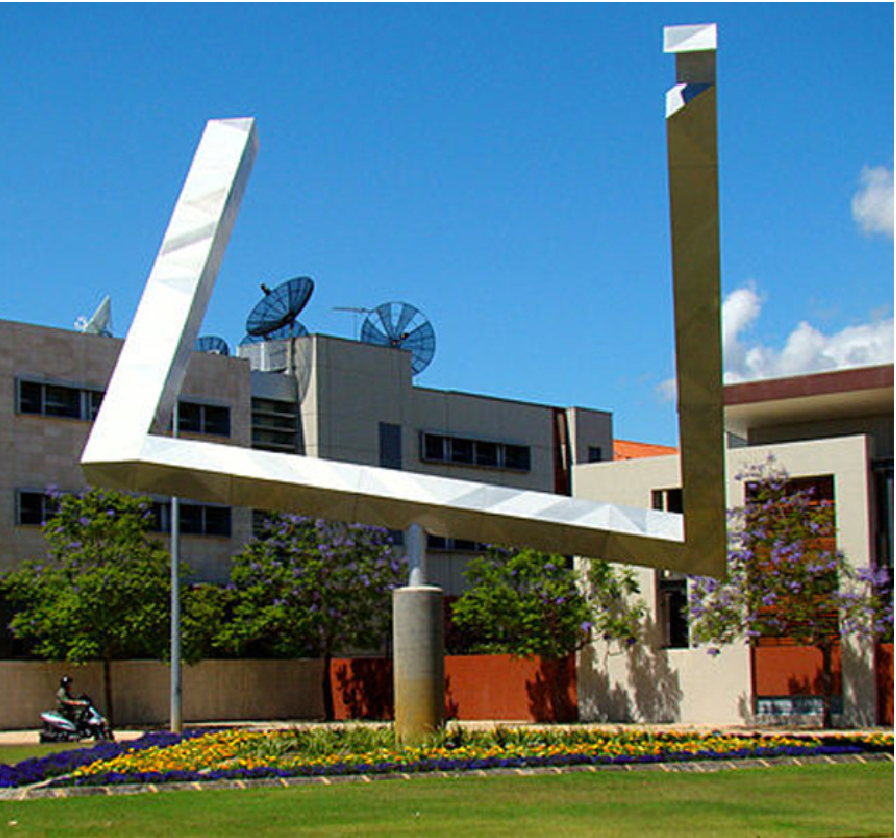
\includegraphics[height=5.5cm]{Penrose1} \qquad 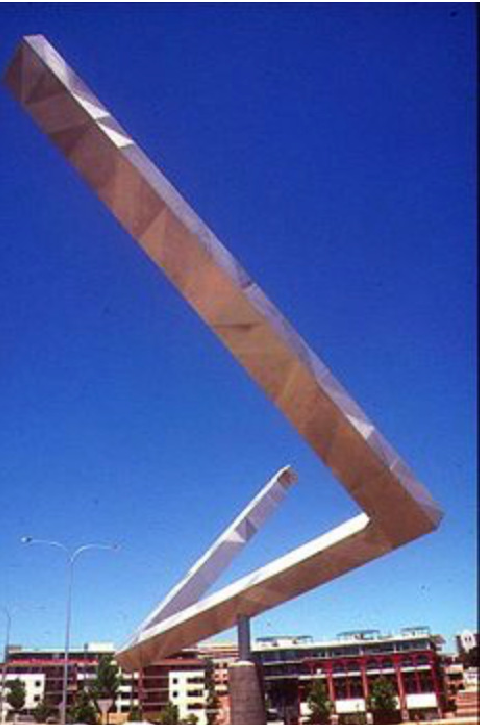
\includegraphics[height=5.5cm]{Penrose2} \qquad 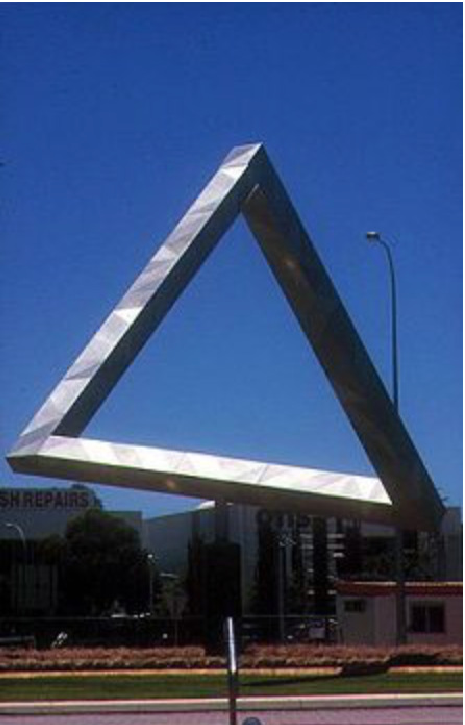
\includegraphics[height=5.5cm]{Penrose3}
         \end{center}

         \vfill\hfill {\footnotesize\it Source : https://im-possible.info/english/}

\end{Maquette}
    \pagebreak
    \graphicspath{{../../S09_Horaires_et_durees/Images}}

\themeM
\chapter{Horaires et durées}
\label{S09}

\programme%
   {\item Connaître les horaire et durées et les relations qui les lient.}
   {\item Mener des calculs impliquant des grandeurs mesurables, exprimer les résultats dans des les unités adaptées.
    \item Exprimer et vérifier la cohérence des résultats du point de vue des unités.}

\vfill

\begin{debat}{Débat : Instruments anciens de mesure de temps et de durée}
   De tous temps on a voulu mesurer le {\bf temps} et la {\bf durée}, ci-dessous figurent quelques instruments utilisés dans des époques plus ou moins lointaines.
   \tcblower
      \begin{tabular}{*{3}{C{5}}}
         
\includegraphics[height=3cm]{cadran}
         &
         
\includegraphics[height=3cm]{clepshydre.png}
         &
         
\includegraphics[height=3cm]{sablier.png} \\
         Cadran solaire & Clepsydre & Sablier \\
         1\,500 av. J.-C. & 1\,600 av. J.-C. & IX\up{e} siècle \\
         Heures du jour & Durées longues (heures) & Durées courtes (minutes) \\
      \end{tabular}
\end{debat}

\hfill {\gray Vidéo : \href{https://www.youtube.com/watch?v=8vMTE9U9z0U}{\bf Remettons les pendules à l'heure}, chaîne YouTube {\it C'est pas sorcier}.}


%%% Approche %%%
\begin{Maquette}[Cours]{Theme={Activité d'approche},Couleur={SteelBlue}}

   \AAtitre{Le temps qui passe}

      {\it Objectifs : donner un ordre de grandeur dans le domaine des durées.}

      \begin{AActivite}

         \AApartie{Les règles du jeu}
            {\singlespacing
            Pour chacune des douze situations numérotées A à L ci-dessous :
            \begin{itemize}
               \item trouver un ordre de grandeur de la durée (seconde, minute, heure, jour, mois, année ou siècle) ;
               \item identifier la couleur correspondante dans le tableau suivant :
                  \begin{center}
                        \begin{tabular}{|>{\columncolor{lightgray}}c|*{7}{C{1.5}|}}
                           \hline
                           Durée & seconde & minute & heure & jour & mois & année & siècle \\
                           \hline
                           Couleur & blanc & beige & noir & jaune & marron & rouge & bleu \\
                           & & \cellcolor{Bisque}{} & \cellcolor{Black}{} & \cellcolor{yellow}{} & \cellcolor{SaddleBrown}{} & \cellcolor{red}{} & \cellcolor{Blue}{} \\
                           \hline
                        \end{tabular}
                  \end{center}
               \item colorier les cases avec le numéro de la situation de la couleur identifiée.
            \end{itemize}}

         \AApartie{À vous de jouer !}
            \begin{multicols}{2}
               {\singlespacing
               \begin{enumerate}[label=\Alph*.]
                  \item Temps mis par la lumière du soleil pour aller jusqu'à la Terre.
                  \item Durée de chacune des quatre saisons.
                  \item Record du monde du \Lg[m]{100}.
                  \item Temps de cuisson d'un \oe uf à la coque.
                  \item Intervalle entre deux battements de c\oe ur consécutifs.
                  \item Durée d'un cycle complet de lune.
                  \item Durée d'un weekend.
                  \item Durée d'un film.
                  \item Temps mis par la Terre pour faire le tour de son étoile : le Soleil.
                  \item Âge maximum atteint par un humain.
                  \item Durée d'une grossesse.
                  \item Durée d'un entraînement de sport.
               \end{enumerate}}
            \end{multicols}
            \begin{center}
               \PixelArt[Unite=4mm,Lettres=ABCDEFGHIJKL,Largeur=18,Hauteur=29,ListeCouleurs={Bisque,Brown,White,Bisque,White,Maroon,Yellow,Black,Red,Blue,Red,Black}]{../../S09_Horaires_et_durees/Images/Mario_duree.csv}
            \end{center}

      \end{AActivite}

\end{Maquette}


%%%Trace écrite %%%
\begin{Maquette}[Cours]{Theme={Trace écrite},Couleur={0.4[SteelBlue,Black]}}

   %%%1
   \section{Unités de temps}

      Selon les situations, on indique les durées en années, mois, jours, heures, minutes, ou secondes : \par
      1 siècle = 100 ans ; 1 an = 12 mois = 365/366 jours ; 1 jour = 24 heures ; 1 heure = 60 minutes = \num{3600} secondes\dots \par
      Pour mesurer le temps ou une durée, on peut utiliser un cadran solaire, un sablier, une montre, un chronomètre\dots

   %%%2
   \section{Conversion de durées}

      La seconde (s) est l'unité du système SI permettant de caractériser une durée. Contrairement aux autres unités, elle ne suit pas un système décimal, mais hexadécimal (de base 60).

      \begin{methode*}{Convertir des durées}
         Pour convertir des heures en minutes ou des minutes en secondes ou inversement, on peut utiliser le schéma suivant : \par
         \begin{pspicture}(-3,-0.5)(11.5,3.5)
            \rnode{A}{\psframebox{durée en heures}}
            \hspace{12mm}
            \rnode{B}{\psframebox{durée en minutes}}
            \hspace{12mm}
            \rnode{C}{\psframebox{durée en secondes}}
            \nccurve[angle=90,linecolor=DodgerBlue,offset=-1mm]{A}{B}
            \naput*{\textcolor{DodgerBlue}{$\stackrel{\times60}{\longrightarrow}$}}
            \nbput*{\textcolor{DodgerBlue}{$\stackrel{\div60}{\longleftarrow}$}}
            \nccurve[angle=90,linecolor=DodgerBlue,offset=-1mm]{->}{B}{C}
            \naput*{\textcolor{DodgerBlue}{$\stackrel{\times60}{\longrightarrow}$}}
            \nbput*{\textcolor{DodgerBlue}{$\stackrel{\div60}{\longleftarrow}$}}
            \nccurve[angle=90,linecolor=Crimson]{->}{A}{C}
            \naput*{\textcolor{Crimson}{$\stackrel{\times3\,600}{\longrightarrow}$}}
            \nbput*{\textcolor{Crimson}{$\stackrel{\div3\,600}{\longleftarrow}$}}
         \end{pspicture}
         \begin{exmethode}
            \begin{itemize}
               \item Convertir 170 minutes en heures et minutes.
               \item Convertir \Temps{;;;1;25;36} en secondes.
            \end{itemize} 
            \tcblower
               \begin{itemize}
                  \item $170=2\times60+50$, donc $\Temps{;;;;170} =\Temps{;;;2;50}$.
                  \item $\Temps{;;;1;25;36} =\Temps{;;;;;3600}+25\times\Temps{;;;;;60}+\Temps{;;;;;36}$ \par
                     $\Temps{;;;1;25;36} =\Temps{;;;;;5136}$.
               \end{itemize}
         \end{exmethode}
      \end{methode*}

      Pour effectuer des additions ou soustractions de durées, on peut effectuer une opération en colonne (un peu périlleuse) ou procéder de proche en proche.
      
      \begin{exemple*}{}
         \begin{itemize}
            \item Un train part de Montpellier à \Temps{;;;8;48}. La durée du trajet pour se rendre à Paris est de \Temps{;;;3;20}. \par
               À quelle heure arrivera-t-il à Paris ? \par
               \qquad
               \begin{tabular}{ccccc}
                  & 8 & h & 4 & 8 \\
                  $+$ & 3 & h & 2 & 0 \\
                  \hline
                  1 & $\cancel{1}$ & h & $\cancel{6}$ & 8 \\
                  \multicolumn{5}{c}{\psline{->}(0.5,0.3)(-0.5,-0.1)} \\
                  1 & 2 & h & 0 & 8
               \end{tabular}
               \qquad
               \begin{tabular}{p{8cm}}
                  \small
                  On aligne les heures sous les heures, les minutes sous les minutes puis on additionne terme à terme. \\ [8mm]
                  Si le nombre de minutes est supérieur à 60, on soustrait 60 minutes et on ajoute 1 heure. \\
               \end{tabular} 
            \item Un automobiliste part de Perpignan à \Temps{;;;8;35} et arrive à Montpellier à \Temps{;;;10;20}. \par
               Quelle est la durée de son trajet ? \par \smallskip
               \qquad \Temps{;;;8;35} $\xrightarrow{+\Temps{;;;;25}}$ \Temps{;;;9;00} $\xrightarrow{+\Temps{;;;1}}$ \Temps{;;;10;00} $\xrightarrow{+\Temps{;;;;20}}$ \Temps{;;;10;20}. \par  
               La durée totale du trajet est de \Temps{;;;1;45}
         \end{itemize} 
      \end{exemple*}

      Remarque : attention à l'aspect hexadécimal de cette grandeur.
         \begin{itemize}
            \item Lorsqu'on lit \Temps{;;;1,5}, cela correspond à \Temps{;;;1} et \Temps{;;;0,5}, c'est-à-dire \Temps{;;;1;30} ($0,5\times\Temps{;;;;60} =\Temps{;;;;30}$).
            \item Inversement, \Temps{;;;2;15} ne correspond pas à \Temps{;;;2,15} mais à \Temps{;;;2,25} ($\Temps{;;;;15} =\dfrac{15}{60}\text{h} =\Temps{;;;0,25}$).
         \end{itemize}

\end{Maquette}


%%% Exercices %%%
\begin{Maquette}[Fiche,CorrigeFin,Colonnes=2]{}

   \begin{multicols}{2}

      \begin{exercice} %1
         Malak part à \Temps{;;;7;38} pour prendre le bus direction le collège Simone Veil. \par
         Elle met 6 minutes pour aller jusqu'à l'arrêt de bus, puis le trajet en bus dure 16 minutes et enfin il lui reste 4 minutes à pied. \par
         À quelle heure arrivera-t-elle au collège ?
      \end{exercice}
      
      \begin{Solution}
         Le temps de déplacement de Malak est de \par
         $\Temps{;;;;6}+\Temps{;;;;16}+\Temps{;;;;4} =\Temps{;;;;26}$. \par
         Or, $\Temps{;;;7;38}+\Temps{;;;;26} =\Temps{;;;7;64} =\Temps{;;;8;4}$. \par
         \cor{Malak devrait arriver au collège à \Temps{;;;8;4}\,\Temps{;;;;04}}.
      \end{Solution}

      
      \begin{exercice} %2
         Hugoline part du collège à pied à \Temps{;;;17;4}. \par
         Elle prévoit \Temps{;;;;15;30} pour le trajet, \Temps{;;;;5} pour acheter un pain au chocolat et \Temps{;;;;7} pour dire au revoir aux copines (et copains !). \par
         À quelle heure arrivera-t-elle chez elle ?
      \end{exercice}
      
      \begin{Solution}
         Le temps de déplacement de Hugoline est de \par
         $\Temps{;;;;15;30}+\Temps{;;;;5}+\Temps{;;;;7} =\Temps{;;;;27;30}$. \par
         Or, $\Temps{;;;17;4}+\Temps{;;;;27;30} =\Temps{;;;17;31;30}$. \par
         \cor{Hugoline devrait arriver chez elle à \Temps{;;;17;31;30}}.
      \end{Solution}
      
      
      \begin{exercice} %3
         Safae part en promenade à \Temps{;;;9;20}. \par
         Elle rentre à \Temps{;;;12;15}, ne s'étant arrêtée pour se reposer que lors de trois pauses de \Temps{;;;;5} chacune. \par
         Pendant combien de temps a-t-elle marché ?
      \end{exercice}
      
      \begin{Solution}
         $\Temps{;;;9;20} \quad \xrightarrow{+\Temps{;;;;40}} \quad \Temps{;;;10;0}$ \par
         $\Temps{;;;10;0} \quad \xrightarrow{+\Temps{;;;2;15}} \quad \Temps{;;;12;15}$ \par
         La promenade de Safae a duré \Temps{;;;2;55}. \par
         Or, il s'est arrêtée $3\times\Temps{;;;;5} =\Temps{;;;;15}$ \par
         donc, \cor{elle a marché durant \Temps{;;;2;40}\,\Temps{;;;;40}}.
      \end{Solution}
      
      
      \begin{exercice} %4
         Convertir les durées données ci-dessous en minutes.
         \begin{enumerate}
            \item \Temps{;;;1;56}.
            \item \Temps{;;2;;25}.
            \item \Temps{;;1;20;3}.
         \end{enumerate}
      \end{exercice}
      
      \begin{Solution}
         \begin{enumerate}
            \item $\Temps{;;;1;56}. =1\times\Temps{;;;;60}+\Temps{;;;;56} =\cor{\Temps{;;;;116}}$.
            \item $\Temps{;;2;;25} =2\times24\times\Temps{;;;;60}+\Temps{;;;;25}$ \par
               \quad $=\Temps{;;;;2880}+\Temps{;;;;25} =\cor{\Temps{;;;;2905}}$.
            \item $\Temps{;;1;20;3} =24\times\Temps{;;;;60}+20\times\Temps{;;;;60}+\Temps{;;;;3}$ \par
               \quad $=\Temps{;;;;1440}+\Temps{;;;;1200}+\Temps{;;;;3} =\cor{\Temps{;;;;2643}}$.
         \end{enumerate}
      \end{Solution}
      
      
      \begin{exercice} %5
         Convertir les durées données ci-dessous en heures et minutes.
         \begin{enumerate}
            \item \Temps{;;;;156}.
            \item \Temps{;;;;296}.
            \item \Temps{;;;;1603}.
         \end{enumerate}
      \end{exercice}
      
      \begin{Solution}
         \begin{enumerate}
            \item $\Temps{;;;;156} =2\times\Temps{;;;;60}+\Temps{;;;;36} =\cor{\Temps{;;;2;36}}$.
            \item $\Temps{;;;;296} =4\times\Temps{;;;;60}+\Temps{;;;;56} =\cor{\Temps{;;;4;46}}$.
            \item $\Temps{;;;;1603} =26\times\Temps{;;;;60}+\Temps{;;;;43}$ \par
               \quad $=\Temps{;;;26;43} =\cor{\Temps{;;1;2;43}}$.
         \end{enumerate}
      \end{Solution}
      
      
      \begin{exercice} %6
         Convertir les durées données ci-dessous en heures et minutes.
         \begin{enumerate}
            \item \Temps{;;;1,5}.
            \item \Temps{;;;2,25}.
            \item \Temps{;;;0,3}.
         \end{enumerate}
      \end{exercice}
      
      \begin{Solution}
         \begin{enumerate}
            \item $\Temps{;;;1,5} =\cor{\Temps{;;;1;30}}$.
            \item $\Temps{;;;2,25} =\cor{\Temps{;;;2;15}}$.
            \item $\Temps{;;;0,3} =0,3\times\Temps{;;;;60} =\cor{\Temps{;;;;18}}$.
         \end{enumerate}
      \end{Solution}
      
      
      \begin{exercice}[Dur] %4
         Convertir les durées données ci-dessous en heures décimales.
         \begin{enumerate}
            \item $\Temps{;;;6;30}$.
            \item $\Temps{;;;2;45}$.
            \item $\Temps{;;;8;33}$.
         \end{enumerate}
      \end{exercice}
      
      \begin{Solution}
         \begin{enumerate}
            \item $\Temps{;;;6;30} =\cor{\Temps{;;;6,5}}$.
            \item $\Temps{;;;2;45} =\cor{\Temps{;;;2,75}}$. \smallskip
            \item $\Temps{;;;8;33} =\Temps{;;;8}+\frac{33}{60}\text{h} =\cor{\Temps{;;;8,55}}$.
         \end{enumerate}
      \end{Solution}
       
      
      \begin{exercice} %8
         Effectuer les calculs suivants :
         \begin{enumerate}
            \item $\Temps{;;;3}\,\Temps{;;;;45}+\Temps{;;;5}\,\Temps{;;;;13}$
            \item $\Temps{;;;5}\,\Temps{;;;;38}+\Temps{;;;9}\,\Temps{;;;;43}$
            \item $\Temps{;;;11}\,\Temps{;;;;28}-\Temps{;;;7}\,\Temps{;;;;22}$
            \item $\Temps{;;;15}\,\Temps{;;;;35}-\Temps{;;;9}\,\Temps{;;;;49}$
         \end{enumerate}
      \end{exercice}
      
      \begin{Solution}
         \begin{enumerate}
            \item $\Temps{;;;3}+\Temps{;;;5} =\Temps{;;;8}$ et $\Temps{;;;;45}+\Temps{;;;;13} =\Temps{;;;;58}$ \par
               donc, $\Temps{;;;3}\,\Temps{;;;;45}+\Temps{;;;5}\,\Temps{;;;;13} =\cor{\Temps{;;;8;58}}$.
            \item $\Temps{;;;5}+\Temps{;;;9} =\Temps{;;;14}$ et \par
               $\Temps{;;;;38}+\Temps{;;;;43} =\Temps{;;;;81} =\Temps{;;;1;21}$ \par
               donc, $\Temps{;;;5;38}+\Temps{;;;9;43} =\cor{\Temps{;;;15;21}}$.
            \item $\Temps{;;;7;22} \quad \xrightarrow{+\Temps{;;;;38}} \quad \Temps{;;;8;0}$ \par
               \quad\, $\Temps{;;;8;0} \quad \xrightarrow{+\Temps{;;;3;28}} \quad \Temps{;;;11;28}$ \par
               $\Temps{;;;11;28}-\Temps{;;;7;22} =\Temps{;;;3;66} =\cor{\Temps{;;;4;6}}$.
            \item $\Temps{;;;9;39} \quad \xrightarrow{+\Temps{;;;;11}} \quad \Temps{;;;10;0}$ \par
               \quad\, $\Temps{;;;10;0} \quad \xrightarrow{+\Temps{;;;5;35}} \quad \Temps{;;;15;35}$ \par  
               $\Temps{;;;15;35}-\Temps{;;;9;49} =\cor{\Temps{;;;5;46}}$.
         \end{enumerate}
      \end{Solution}


      \begin{exercice} %9
         Dans une usine, une machine met \Temps{;;;;5;26} pour fabriquer une pièce.
         \begin{enumerate}
            \item Combien de temps met-elle pour fabriquer 5 pièces ?
            \item Combien de temps met-elle pour en fabriquer 10 ?
            \item Combien de temps met-elle pour en fabriquer 20 ?
            \item Combien de temps met-elle pour en fabriquer 100 ?
            \item Combien la machine aura-t-elle fabriqué de pièces si elle fonctionne \Temps{;;;8} sans s’arrêter ?
            \item Une nouvelle machine, qui vient d’arriver, met deux fois moins de temps pour fabriquer la même pièce. Quel temps met-elle pour fabriquer la pièce ?
         \end{enumerate}
      \end{exercice}
      
      \begin{Solution}
         \begin{enumerate}
            \item $5\times\Temps{;;;;5} =\Temps{;;;;25}$ et $5\times\Temps{;;;;;26} =\Temps{;;;;;130} =\Temps{;;;;2;10}$. \par
               $\Temps{;;;;25}+\Temps{;;;;2;10} =\cor{\Temps{;;;;27;10}}$.
            \item $2\times(\Temps{;;;;27;10}) =\cor{\Temps{;;;;54;20}}$.
            \item $2\times(\Temps{;;;;54;20}) =\Temps{;;;;108;40} =\cor{\Temps{;;;1;48;40}}$.
            \item $10\times(\Temps{;;;;54;20}) =\Temps{;;;;540;200} =\cor{\Temps{;;;9;3;20}}$.
            \item $\Temps{;;;8} =8\times\Temps{;;;;;3600} =\Temps{;;;;;28800}$ \par
               et $\Temps{;;;;5;26} =5\times\Temps{;;;;;60}+\Temps{;;;;;26} =\Temps{;;;;;326}$. \par
               Or, $\num{28800}\div326 \approx88,34$ donc, \cor{la machine aura fabriqué 88 pièces en \Temps{;;;8}}.
            \item La moitié de \Temps{;;;;5} vaut \Temps{;;;;2;30} et la moitié de \Temps{;;;;;26} vaut \Temps{;;;;;13} donc, \cor{la machine met \Temps{;;;;2;43}}.
         \end{enumerate}
      \end{Solution}
      
      
      \begin{exercice}[Dur] %10
         Résolution de problème : des robinets qui coulent. \par
         On dispose de deux robinets.
         \begin{itemize}
            \item Le premier est capable de remplir un réservoir d’eau de \Capa{24} en 1 minute.
            \item Le second peut remplir ce même réservoir en 2 minutes.
         \end{itemize}
         En ouvrant les deux robinets au même moment, combien de temps faudrait-il pour remplir un jacuzzi avec \Capa{1080} d’eau ? \par
         \begin{minipage}{4cm}
            \begin{enumerate}
               \item[a.] 15 min.
               \item[b.] 67,5 min.
               \item[c.] 135 min.
               \item[d.] 30 min.
            \end{enumerate}
         \end{minipage}
         \begin{minipage}{2cm}
            
\includegraphics[width=2cm]{robinet}
         \end{minipage}
      \end{exercice}
      
      \begin{Solution}
         Pour un volume à remplir, le robinet R1 met deux fois moins de temps que le robinet R2. Donc, pendant le temps total, R1 remplit deux \og unités de volume \fg{} pendant que R2 n'en remplit qu’une : \par \smallskip
         \ModeleBarre[Largeur=2.5cm]{PowderBlue 3 {"\Capa{1080}"}}{DeepSkyBlue 1 "R1" DeepSkyBlue 1 "R1" LightSkyBlue 1 "R2"} \par
         En partageant le volume total en trois parties égales, on trouve $\Capa{1080}\div3 =\Capa{360}$. \par
         R2 remplit un tiers du volume total du jacuzzi : \Capa{360}. \par
         Or, $360\div12 =30$. Sachant que R2 remplit \Capa{12} en \Temps{;;;;1}, il remplit \Capa{360} en \Temps{;;;;30}. \par
         \cor{La réponse est 30 minutes (d)}.
      \end{Solution}

   \end{multicols}

\end{Maquette}


%%% Récré %%%
\begin{Maquette}[Cours]{Theme={Activité récréative},Couleur={IndianRed}}
    
   \ARtitre{L'horloge de Mengenlehreuhr}

      \ARpartie{Présentation}  
         La {\bf Mengenlehreuhr} (en allemand \og Horloge de la théorie du jeu \fg) ou {\bf Berlin-Uhr} (\og Horloge de Berlin \fg) est la première horloge publique au monde qui indique l'heure au moyen de champs lumineux colorés, ce qui lui a valu d'entrer dans le livre Guinness des records lors de son installation le 17 juin 1975. \par
         \hfill{\it \small Source : \href{https://en.wikipedia.org/wiki/Mengenlehreuhr}{wikipedia}}

      \ARpartie{recherche}
         À partir des images suivantes représentant l'horloge à différents moments de la journée, déterminer le fonctionnement de l'horloge. Par groupe, vous construirez une affiche récapitulant vos recherches.
         \vfill
         \begin{center}
            {\psset{unit=0.54}
            \begin{minipage}{6cm}  
               \begin{pspicture}(0,-1.5)(11,13.8)
                  \rput(5.5,6.5){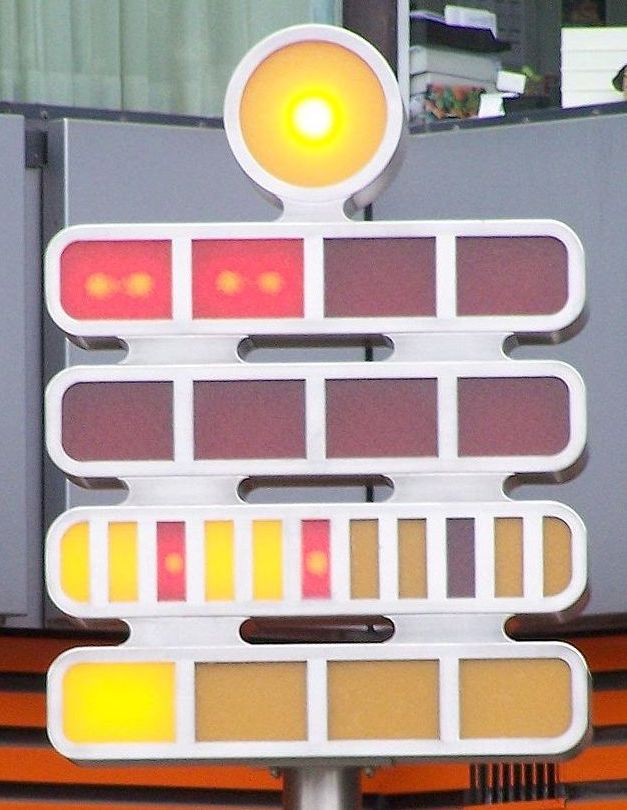
\includegraphics[width=6.7cm]{horloge_Berlin}}
               \end{pspicture}
            \end{minipage}
            \hspace{3cm}
            \begin{minipage}{6cm}  
               \begin{pspicture}(0,-1)(11,13.8)
                  \psset{linecolor=yellow,fillstyle=solid,framearc=0.35}
                     \psframe*(0,0)(2.75,2) %m1
                     \psframe*(0,2.8)(5,4.8) %m5
                     \pscircle*(5.5,12.54){1.6}
                  \psset{linecolor=OrangeRed}
                     \psframe*(2,2.8)(3,4.8) \psframe*(5,2.8)(6,4.8) %mi
                     \psframe*(0,8.4)(5.5,10.4) %h5  
                  \horloge
                  \rput(5.5,-1){\large Il est 10h31}
               \end{pspicture}
            \end{minipage}
            \vfill
            \begin{minipage}{6cm}  
               \begin{pspicture}(0,-1)(11,15.5)
                  \psset{linecolor=yellow,fillstyle=solid,framearc=0.35}
                     \psframe*(0,0)(2.75,2) %m1
                     \psframe*(0,2.8)(1,4.8) %m5
                  \psset{linecolor=OrangeRed}
                     \psframe*(0,5.6)(2.75,7.6) %h1
                     \psframe*(0,8.4)(2.75,10.4) %h5  
                  \horloge
                  \rput(5.5,-1){\large Il est 6h06}
               \end{pspicture}
            \end{minipage}
            \hspace{3cm}
            \begin{minipage}{6cm}  
               \begin{pspicture}(0,-1)(11,15)
                  \psset{linecolor=yellow,fillstyle=solid,framearc=0.35}
                     \psframe*(0,2.8)(11,4.8) %m5
                  \psset{linecolor=OrangeRed}
                     \psframe*(2,2.8)(3,4.8) \psframe*(5,2.8)(6,4.8) \psframe*(8,2.8)(9,4.8) %mi
                     \psframe*(0,5.6)(8.25,7.6) %h1
                  \horloge
                  \rput(5.5,-1){\large Il est 3h55}
               \end{pspicture}
            \end{minipage}
            \vfill}
         \end{center}

\end{Maquette}
    \pagebreak
    \graphicspath{{../../S10_Comparaison_et_egalite_de_fractions/Images/}}

\themeN
\chapter{Comparaison et égalité de fractions} \label{S10}

\programme%
   {\item Fractions, nombres rationnels.
   \item Égalité de fractions.
   \item Ordre sur les nombres rationnels.}
   {\item Comparer, ranger, encadrer des nombres fractionnaires.
   \item Repérer et placer un nombre rationnel sur une droite graduée.}

\vfill

\begin{debat}{Débat : les fractions, ces nombres rompus !}
   Tout nombre peut s'écrire de différentes façons : ils ont des habillages différents mais ont la même valeur. La façon dont on les écrit permet de pouvoir les comparer. Par exemple, la {\bf fraction} $\dfrac68$ possède (entre autres) les représentations suivantes :
   \tcblower
      {\psset{unit=0.8}
      \begin{pspicture}(-4,-4)(4,4)  
         {\large
         \multido{\n=5+60,\i=55+60}{6}{\psline(3;\n)(0,0)(3;\i)}
         \multido{\n=30+60,\i=-60+60,\r=120+60}{6}{\psarc(2.719;\n){1.268}{\i}{\r}}
         \pscircle[fillstyle=solid,fillcolor=yellow](0,0){1.3}
         \rput(0,0){\bf $\dfrac68$}
         \rput(2.7;30){75\,\%}
         \rput(2.7;-30){0,75}
         \rput(2.7;150){$\dfrac34$}
         \rput(2.7;-150){$\dfrac{75}{100}$}
         \rput(2.7;90){\pswedge[fillstyle=solid,fillcolor=Crimson](0,0){0.8}{0}{-90}
                              \pscircle(0,0){0.8}
                              \multido{\n=0+45}{8}{\psline(0,0)(0.8;\n)}}
         \rput(2.7;-90){\psline(-1,0)(1,0)  
         \rput(-1,-0.4){\footnotesize 0}
         \rput(1,-0.4){\footnotesize 1}
         \psline[linecolor=Crimson,linewidth=1mm](-1,0)(0.5,0) \multido{\r=-1+0.25}{9}{\rput(\r,0){|}}}}
      \end{pspicture}}
\end{debat}

\hfill {\gray Vidéo : \href{https://www.youtube.com/watch?v=eawBr43xWf8}{\bf Les fractions}, chaîne Youtube {\it Petits contes mathématiques}.}


%%% Approche %%%
\begin{Maquette}[Cours]{Theme={Activité d'approche},Couleur={SteelBlue}}

   \AAtitre{Des briques et des fractions}

      {\it Objectifs : utiliser des fractions pour exprimer une proportion ; produire des fractions égales, ranger des fractions.}

      \begin{AActivite}

         \AApartie{Les Lego®}
            \begin{minipage}{10cm}
               On choisit la brique de Lego® classique $u$ ci-contre que l'on prend comme unité et les onze briques $a$ à $k$. \par
               On considère que le volume d'une brique est proportionnel au nombre de \og boutons \fg{} présents sur le dessus.
            \end{minipage}
            \hspace{1cm}
            \begin{minipage}{5cm}
               $u$ : 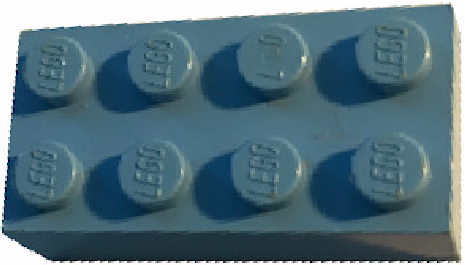
\includegraphics[width=3.15cm]{lego_4_2a}
            \end{minipage} \par \bigskip
               $a$ : 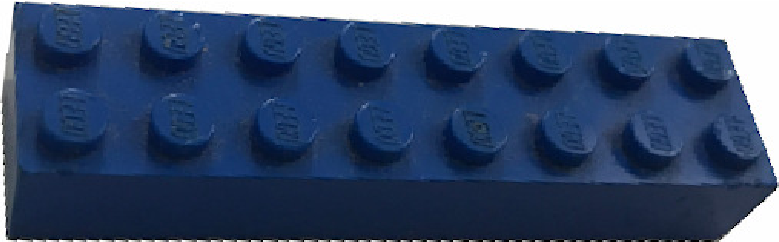
\includegraphics[width=5.22cm]{lego_8_2a} \qquad 
               $b$ : 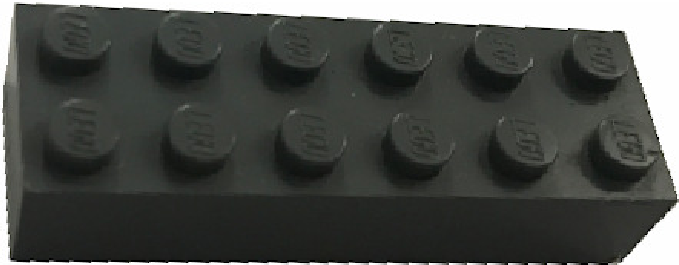
\includegraphics[width=3.6cm]{lego_6_2a} \qquad
               $c$ : 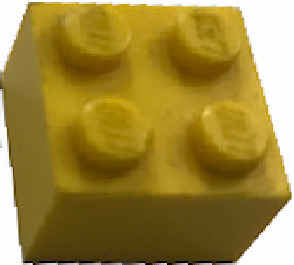
\includegraphics[width=1.35cm]{lego_2_2a} \qquad
               $d$ : 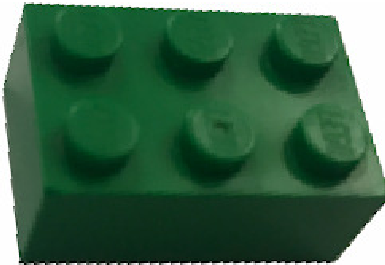
\includegraphics[width=1.8cm]{lego_3_2a} \\ [5mm]
               $e$ : 
\includegraphics[width=6.3cm]{lego_10_2a} \qquad
               $f$ : 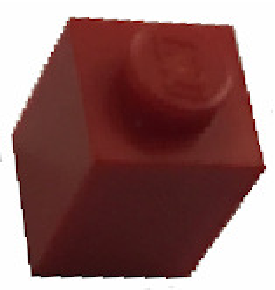
\includegraphics[width=0.9cm]{lego_1_1a} \qquad
               $g$ : 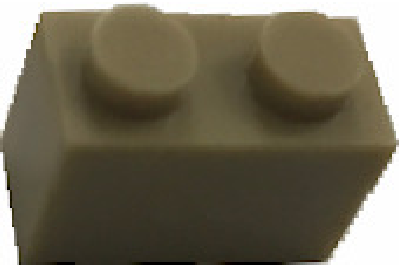
\includegraphics[width=1.35cm]{lego_2_1a} \qquad
               $h$ : 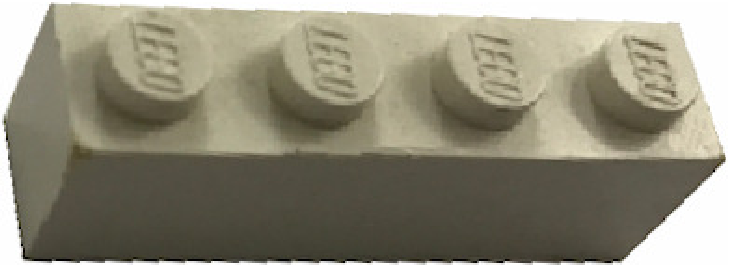
\includegraphics[width=2.7cm]{lego_4_1a} \\ [5mm]
               $i$ : 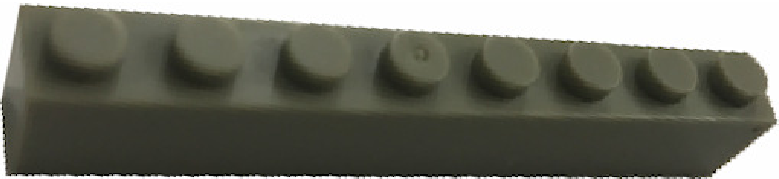
\includegraphics[width=5.4cm]{lego_8_1a} \qquad
               $j$ : 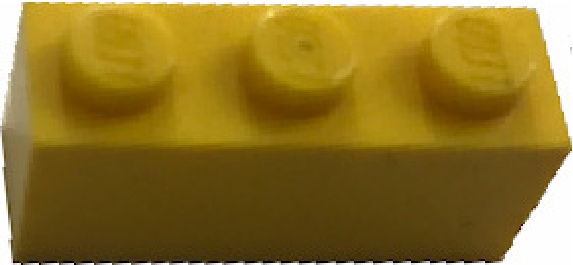
\includegraphics[width=1.98cm]{lego_3_1a} \qquad
               $k$ : 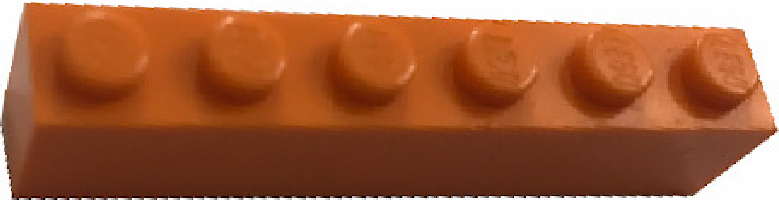
\includegraphics[width=4.05cm]{lego_6_1a} \bigskip
               
         \AApartie{Les fractions}
            \begin{enumerate}
               \item Compléter les égalités suivantes à l'aide de nombres fractionnaires : \par \bigskip
                  \begin{multicols}{6}
                     $a = \pointilles u$ \par \vskip8mm
                     $g = \pointilles u$ \par \vskip8mm
                     $b = \pointilles u$ \par \vskip8mm
                     $h = \pointilles u$ \par \vskip8mm
                     $c = \pointilles u$ \par \vskip8mm
                     $i = \pointilles u$ \par \vskip8mm
                     $d = \pointilles u$ \par \vskip8mm
                     $j = \pointilles u$ \par \vskip8mm
                     $e = \pointilles u$ \par \vskip8mm
                     $k = \pointilles u$ \par \vskip8mm
                     $f = \pointilles u$ \par \vskip8mm
                  \end{multicols} \vskip8mm
               \item Compléter les égalités suivantes à l'aide de fractions dont le dénominateur est 8 : \par \bigskip
                  \begin{multicols}{6}
                     $a = \dfrac{\pointilles[1cm]}{8} u$ \par \vskip8mm
                     $g = \dfrac{\pointilles[1cm]}{8} u$ \par \vskip8mm
                     $b = \dfrac{\pointilles[1cm]}{8} u$ \par \vskip8mm
                     $h = \dfrac{\pointilles[1cm]}{8} u$ \par \vskip8mm
                     $c = \dfrac{\pointilles[1cm]}{8} u$ \par \vskip8mm
                     $i = \dfrac{\pointilles[1cm]}{8} u$ \par \vskip8mm
                     $d = \dfrac{\pointilles[1cm]}{8} u$ \par \vskip8mm
                     $j = \dfrac{\pointilles[1cm]}{8} u$ \par \vskip8mm
                     $e = \dfrac{\pointilles[1cm]}{8} u$ \par \vskip8mm
                     $k = \dfrac{\pointilles[1cm]}{8} u$ \par \vskip8mm
                     $f = \dfrac{\pointilles[1cm]}{8} u$ \par \vskip8mm
                  \end{multicols} \vskip8mm
               \item Classer les Lego® dans l'ordre croissant de leur volume : \par \vskip5mm
                  \pointilles \par \vskip7mm
                  \pointilles \par \bigskip
         \end{enumerate}

   \end{AActivite}

\end{Maquette}


%%%Trace écrite %%%
\begin{Maquette}[Cours]{Theme={Trace écrite},Couleur={0.4[SteelBlue,Black]}}

   %%%1
   \section{Égalité de fractions}

      \begin{propriete*}{}
         On ne change pas la valeur d'une fraction en multipliant ou en divisant le numérateur et le dénominateur par un même nombre relatif non nul.
         $$\dfrac{b}{c} =\dfrac{b\times a}{c\times a}= \dfrac{ba}{ca}. \text{\quad On a aussi \quad }a\times\dfrac{b}{c}= \dfrac{a\times b}{c} =\dfrac{ab}{c}$$
      \end{propriete*}

      Démonstration :\qquad
         {\hautab{1.7}
         \begin{tabular}{p{4cm}p{10cm}}
            $(a\times c)\times\dfrac{b}{c} =a\times \left(c\times\dfrac{b}{c}\right)$
            &
            {\it associativité de la multiplication} \\
            $(a\times c)\times\dfrac{b}{c} =a\times b$
            &
            {\it $\dfrac{b}{c}$ est le nombre qui, multiplié par $c$ donne $b$ donc $c\times\dfrac{b}{c} =b$} \\
            donc, $\dfrac{b}{c} =\dfrac{a\times b}{a\times c}$
            &
            {\it puisque $\dfrac{a\times b}{a\times c}$ est le nombre qui, multiplié par $a\times c$ donne $a\times b$} \\
         \end{tabular}}

      \begin{exemple*}{}   
         $$\dfrac12 =\dfrac{1\times2}{2\times2} =\dfrac24 =\dfrac{2\times2}{4\times2} = \dfrac48\dots \qquad ; \qquad 7\times\dfrac{3}{5} =\dfrac{7\times3}{5} =\dfrac{21}{5}$$
      \end{exemple*}

      Remarque : la propriété permet de {\bf simplifier} des fractions, ce qui  signifie écrire une fraction qui lui est égale, mais avec un numérateur et un dénominateur plus petits.

      \begin{exemple*}{}
         Pour simplifier $\dfrac{150}{180}$, on peut diviser le numérateur et le dénominateur par 10 : $\dfrac{150}{180} =\dfrac{150\div10}{180\div10} =\dfrac{15}{18}$ \par \smallskip
         puis les diviser encore par 3 : $\dfrac{15}{18} =\dfrac{15\div3}{18\div3} =\dfrac56$.
      \end{exemple*}


   %%%2
   \section{Comparaison de fractions}

      \begin{methode*}{Comparer des fractions}
         Pour comparer deux fractions ayant le même dénominateur, il suffit de comparer les numérateurs : la fraction ayant le plus grand numérateur est la plus grande.
         \begin{exmethode}
            Comparer $\dfrac26$ et $\dfrac36$ \; : \; \parbox{1.4cm}{\Fraction[Rayon=6mm,Couleur=SteelBlue,Reponse]{2/6}} et \; \parbox{1.2cm}{\Fraction[Rayon=6mm,Couleur=SteelBlue,Reponse]{3/6}}
            \tcblower
               $2<3$ donc $\dfrac26<\dfrac36$
         \end{exmethode}
         Pour comparer deux fractions de dénominateurs multiples, on modifie l'écriture de l'une des fractions pour qu'elle ait le même dénominateur que l'autre.
         \begin{exmethode}
            Comparer $\dfrac23$ et $\dfrac{7}{12}$ \; : \; \parbox{1.4cm}{\Fraction[Rayon=6mm,Couleur=SteelBlue,Reponse]{2/3}} et \; \parbox{1.2cm}{\Fraction[Rayon=6mm,Couleur=SteelBlue,Reponse]{7/12}}
            \tcblower
               $\dfrac23=\dfrac{2\times4}{3\times4}=\dfrac{8}{12}$ \; : \; \parbox{1.4cm}{\Fraction[Rayon=6mm,Couleur=SteelBlue,Reponse]{2/3}} = \; \parbox{1.2cm}{\Fraction[Rayon=6mm,Couleur=SteelBlue,Reponse]{8/12}} \par \medskip
               $\dfrac{8}{12}>\dfrac{7}{12}$ donc, $\dfrac23>\dfrac{7}{12}$ \; : \; \parbox{1.4cm}{\Fraction[Rayon=6mm,Couleur=SteelBlue,Reponse]{8/12}} > \; \parbox{1.2cm}{\Fraction[Rayon=6mm,Couleur=SteelBlue,Reponse]{7/12}}
         \end{exmethode}
      \end{methode*}

\end{Maquette}


%%% Exercices %%%
\begin{Maquette}[Fiche,CorrigeFin,Colonnes=2]{}
   
   \begin{multicols}{2}

      \begin{exercice}[SLF] %1
         Écrire la fraction qui représente la partie colorée de chaque figure puis la simplifier si possible.
         \begin{center}
            a \Fraction[Regulier,Cotes=4,Rayon=6mm,Couleur=Cyan,Reponse]{1/4} \quad b \Fraction[Regulier,Cotes=4,Rayon=6mm,Couleur=Cyan,Reponse]{3/4} \quad c \Fraction[Regulier,Cotes=4,Rayon=6mm,Couleur=Cyan,Reponse]{2/4} \quad d\Fraction[Regulier,Cotes=4,Rayon=6mm,Couleur=Cyan,Reponse]{4/4} \par \bigskip
            e \Fraction[Rayon=6mm,Couleur=IndianRed,Reponse]{10/12} \quad f \Fraction[Rayon=6mm,Couleur=IndianRed,Reponse]{3/12} \quad g \Fraction[Rayon=6mm,Couleur=IndianRed,Reponse]{2/12} \quad h \Fraction[Rayon=6mm,Couleur=IndianRed,Reponse]{6/12} \par \bigskip
            i \Fraction[Triangle,Longueur=12mm,Couleur=LimeGreen,Reponse]{3/9} \quad j \Fraction[Triangle,Longueur=12mm,Couleur=LimeGreen,Reponse]{7/9} \quad k \Fraction[Triangle,Longueur=12mm,Couleur=LimeGreen,Reponse]{6/9} \quad l \Fraction[Triangle,Longueur=12mm,Couleur=LimeGreen,Reponse]{8/9} \par \bigskip
            {\psset{unit=0.6}
            \begin{pspicture}(-1,-1.4)(2.2,1.2)
               \psgrid[subgriddiv=2,subgridcolor=black,subgridwidth=0.8pt,gridlabels=0](-1,-1)(1,1)
               \psframe[fillstyle=solid,fillcolor=DarkOrange](-1,0)(0,1)
               \rput(-1.4,-0.9){m}
            \end{pspicture}
            \begin{pspicture}(-1,-1.4)(2.2,1.2)
               \psgrid[subgriddiv=2,subgridcolor=black,subgridwidth=0.8pt,gridlabels=0](-1,-1)(1,1)
               \psframe[fillstyle=solid,fillcolor=DarkOrange](-1,0)(0,1)
               \psframe[fillstyle=solid,fillcolor=DarkOrange](0,0.5)(0.5,0)
               \psframe[fillstyle=solid,fillcolor=DarkOrange](-1,-0.5)(-0.5,0)
               \rput(-1.4,-0.9){n}
            \end{pspicture}
            \begin{pspicture}(-1,-1.4)(2.2,1.2)
               \psgrid[subgriddiv=2,subgridcolor=black,subgridwidth=0.8pt,gridlabels=0](-1,-1)(1,1)
               \psframe[fillstyle=solid,fillcolor=DarkOrange](-1,-1)(1,0)
               \psframe[fillstyle=solid,fillcolor=DarkOrange](-1,0)(0,1)
               \psframe[fillstyle=solid,fillcolor=DarkOrange](0,0)(0.5,0.5)
               \rput(-1.4,-0.9){p}
            \end{pspicture}
            \begin{pspicture}(-1,-1.4)(1,1.2)
               \psgrid[subgriddiv=2,subgridcolor=black,subgridwidth=0.8pt,gridlabels=0](-1,-1)(1,1)
               \psframe[fillstyle=solid,fillcolor=DarkOrange](-1,-1)(0.5,0)
               \psframe[fillstyle=solid,fillcolor=DarkOrange](-1,0)(-0.5,1)
               \psframe[fillstyle=solid,fillcolor=DarkOrange](0.5,-0.5)(1,0)
               \rput(-1.4,-0.9){q}
            \end{pspicture}}   
         \end{center}
      \end{exercice}
            
      \begin{Solution}
         \begin{colenumerate}[3][label=\alph*]
            \item $\cor{\dfrac14}$ \medskip
            \item $\cor{\dfrac34}$ \medskip
            \item $\cor{\dfrac24 =\dfrac12}$ \medskip
            \item $\cor{\dfrac44 =1}$ \medskip
            \item $\cor{\dfrac{10}{12} =\dfrac56}$ \medskip
            \item $\cor{\dfrac{3}{12} =\dfrac14}$
            \item $\cor{\dfrac{2}{12} =\dfrac16}$
            \item $\cor{\dfrac{6}{12} =\dfrac12}$
            \item $\cor{\dfrac39 =\dfrac13}$
            \item $\cor{\dfrac79}$
            \item $\cor{\dfrac69 =\dfrac23}$
            \item $\cor{\dfrac89}$
            \item $\cor{\dfrac{4}{16} =\dfrac14}$
            \item $\cor{\dfrac{6}{16} =\dfrac38}$
            \item $\cor{\dfrac{13}{16}}$
            \item $\cor{\dfrac{9}{16}}$
         \end{colenumerate}
      \end{Solution}
          
               
      \begin{exercice}[SLF] %2
         Dans chaque figure, colorier la fraction donnée.
         \begin{center}
         {\small
            \psset{unit=0.75}
            \begin{pspicture}(-1,-1.3)(2.5,1)
               \psframe(-1,-1)(1,1)
               \rput(1.25,0){$\dfrac13$}
            \end{pspicture}
            \begin{pspicture}(-1,-1.3)(2.5,1)
               \psframe(-1,-1)(1,1)
               \rput(1.25,0){$\dfrac34$}
            \end{pspicture}
            \begin{pspicture}(-1,-1.3)(1.5,1)
               \psframe(-1,-1)(1,1)
               \rput(1.25,0){$\dfrac58$}
            \end{pspicture} \\ \medskip
            
            \begin{pspicture}(-1,-1.3)(2.5,1)
               \pscircle(0,0){1}
               \rput(1.25,0){$\dfrac13$}
            \end{pspicture}
            \begin{pspicture}(-1,-1.3)(2.5,1)
               \pscircle(0,0){1}
               \rput(1.25,0){$\dfrac34$}
            \end{pspicture}
            \begin{pspicture}(-1,-1.3)(1.5,1)
               \pscircle(0,0){1}
               \rput(1.25,0){$\dfrac58$}
            \end{pspicture} \\ \medskip
            
            \begin{pspicture}(-1,-1.3)(2.5,1)
               \pspolygon(1;0)(1;60)(1;120)(1;180)(1;-120)(1;-60)
               \rput(1.25,0){$\dfrac13$}
            \end{pspicture}
            \begin{pspicture}(-1,-1.3)(2.5,1)
               \pspolygon(1;0)(1;60)(1;120)(1;180)(1;-120)(1;-60)
               \rput(1.25,0){$\dfrac34$}
            \end{pspicture}
            \begin{pspicture}(-1,-1.3)(1.5,1)
               \pspolygon(1;0)(1;60)(1;120)(1;180)(1;-120)(1;-60)
               \rput(1.25,0){$\dfrac56$}
            \end{pspicture} \\ \medskip
      
            \begin{pspicture}(-1,-1.3)(2.5,1)
               \pspolygon(-1,-0.33)(-1,0.33)(-0.33,0.33)(-0.33,1)(0.33,1)(0.33,0.33)(1,0.33)(1,-0.33)(0.33,-0.33)(0.33,-1)(-0.33,-1)(-0.33,-0.33)
               \rput(1.25,0){$\dfrac14$}
            \end{pspicture}
            \begin{pspicture}(-1,-1.3)(2.5,1)
               \pspolygon(-1,-0.33)(-1,0.33)(-0.33,0.33)(-0.33,1)(0.33,1)(0.33,0.33)(1,0.33)(1,-0.33)(0.33,-0.33)(0.33,-1)(-0.33,-1)(-0.33,-0.33)
               \rput(1.25,0){$\dfrac38$}
            \end{pspicture}
            \begin{pspicture}(-1,-1.3)(1.5,1)
               \pspolygon(-1,-0.33)(-1,0.33)(-0.33,0.33)(-0.33,1)(0.33,1)(0.33,0.33)(1,0.33)(1,-0.33)(0.33,-0.33)(0.33,-1)(-0.33,-1)(-0.33,-0.33)
               \rput(1.25,0){$\dfrac25$}
            \end{pspicture}}
         \end{center}
      \end{exercice}
      
      \begin{Solution}
         \smallskip
         \Fraction[Rectangle,Longueur=12mm,Largeur=12mm,Couleur=CornflowerBlue,Reponse]{1/3} $\dfrac13$ \qquad \Fraction[Rectangle,Multiple=2,Longueur=12mm,Largeur=12mm,Couleur=CornflowerBlue,Reponse]{3/4} $\dfrac34$ \qquad \Fraction[Rectangle,Multiple=2,Longueur=12mm,Largeur=12mm,Couleur=CornflowerBlue,Reponse]{5/8} $\dfrac58$ \par
         \Fraction[Rayon=6mm,Couleur=CornflowerBlue,Reponse]{1/3} $\dfrac13$ \qquad \Fraction[Rayon=6mm,Couleur=CornflowerBlue,Reponse]{3/4} $\dfrac34$ \qquad \Fraction[Rayon=6mm,Couleur=CornflowerBlue,Reponse]{5/8} $\dfrac58$ \par
         \Fraction[Regulier,Cotes=6,Rayon=6mm,Couleur=CornflowerBlue,Reponse]{1/3} $\dfrac13$ \qquad \Fraction[Regulier,Cotes=6,Rayon=6mm,Couleur=CornflowerBlue,Reponse]{3/4} $\dfrac34$ \qquad \Fraction[Regulier,Cotes=6,Rayon=6mm,Couleur=CornflowerBlue,Reponse]{5/6} $\dfrac56$ \par
         {\small
            \psset{unit=0.6}
            \begin{pspicture}(-1,-1.5)(3,1)
               \pspolygon[fillstyle=solid,fillcolor=CornflowerBlue](0,0)(0.33,0.33)(0.33,1)(-0.33,1)(-0.33,0.33)
               \pspolygon(-1,-0.33)(-1,0.33)(-0.33,0.33)(-0.33,1)(0.33,1)(0.33,0.33)(1,0.33)(1,-0.33)(0.33,-0.33)(0.33,-1)(-0.33,-1)(-0.33,-0.33)
               \psline(-0.33,-0.33)(0.33,0.33)
               \psline(0.33,-0.33)(-0.33,0.33)
               \rput(1.5,-1){$\dfrac14$}
            \end{pspicture}
            \begin{pspicture}(-1,-1.5)(3,1)
               \pspolygon[fillstyle=solid,fillcolor=CornflowerBlue](0,0)(1,0)(1,0.33)(0.33,0.33)(0.33,1)(-0.33,1)(-0.33,0.33)
               \pspolygon(-1,-0.33)(-1,0.33)(-0.33,0.33)(-0.33,1)(0.33,1)(0.33,0.33)(1,0.33)(1,-0.33)(0.33,-0.33)(0.33,-1)(-0.33,-1)(-0.33,-0.33)
               \pspolygon(-1,-0.33)(-1,0.33)(-0.33,0.33)(-0.33,1)(0.33,1)(0.33,0.33)(1,0.33)(1,-0.33)(0.33,-0.33)(0.33,-1)(-0.33,-1)(-0.33,-0.33)
               \psline(-0.33,-0.33)(0.33,0.33)
               \psline(0.33,-0.33)(-0.33,0.33)
               \psline(-1,0)(1,0)
               \psline(0,-1)(0,1)
               \rput(1.5,-1){$\dfrac38$}
            \end{pspicture}
            \begin{pspicture}(-1,-1.5)(1.5,1)
               \psframe[fillstyle=solid,fillcolor=CornflowerBlue](-0.33,-0.33)(1,0.33)
               \pspolygon(-1,-0.33)(-1,0.33)(-0.33,0.33)(-0.33,1)(0.33,1)(0.33,0.33)(1,0.33)(1,-0.33)(0.33,-0.33)(0.33,-1)(-0.33,-1)(-0.33,-0.33)
               \psframe(-0.33,-0.33)(0.33,0.33)
               \rput(1.5,-1){$\dfrac25$}
            \end{pspicture}}
      \end{Solution}
           
         
      \begin{exercice}[SLF] %3
         Compléter les fractions suivantes : \medskip
         \begin{enumerate}
            \item $\dfrac{1}{2} =\dfrac{\qquad\;}{14} =\dfrac{8}{\qquad\;} =\dfrac{\qquad\;}{50} =\dfrac{16}{\qquad\;} =\dfrac{64}{\qquad\;}$ \\ [2mm]
            \item $\dfrac{4}{5} =\dfrac{\qquad\;}{15} =\dfrac{8}{\qquad\;} =\dfrac{\qquad\;}{50} =\dfrac{16}{\qquad\;} =\dfrac{64}{\qquad\;}$ \\ [2mm]
            \item $\dfrac{11}{7} =\dfrac{\qquad\;}{14} =\dfrac{88}{\qquad\;} =\dfrac{\qquad\;}{49} =\dfrac{121}{\qquad\;} =\dfrac{550}{\qquad\;}$ \\
         \end{enumerate}
      \end{exercice}
      
      \begin{Solution}
         \begin{enumerate}
            \item $\dfrac{1}{2} =\dfrac{\cor{7}}{14} =\dfrac{8}{\cor{16}} =\dfrac{\cor{25}}{50} =\dfrac{16}{\cor{32}} =\dfrac{64}{\cor{128}}$ \par
            \item $\dfrac{4}{5} =\dfrac{\cor{12}}{15} =\dfrac{8}{\cor{10}} =\dfrac{\cor{40}}{50} =\dfrac{16}{\cor{20}} =\dfrac{64}{\cor{80}}$ \par
            \item $\dfrac{11}{7} =\dfrac{\cor{22}}{14} =\dfrac{88}{\cor{56}} =\dfrac{\cor{77}}{49} =\dfrac{121}{\cor{77}} =\dfrac{550}{\cor{350}}$
         \end{enumerate}
      \end{Solution}
         
         
      \begin{exercice} %4
         Simplifier au maximum ces fractions. \medskip
         \begin{colenumerate}[4]
            \item $\dfrac{6}{10}$ \bigskip
            \item $\dfrac{18}{16}$ \bigskip
            \item $\dfrac{16}{28}$
            \item $\dfrac{30}{48}$
            \item $\dfrac{88}{33}$
            \item $\dfrac{55}{30}$
            \item $\dfrac{15}{75}$
            \item $\dfrac{108}{117}$
         \end{colenumerate}
      \end{exercice}
      
      \begin{Solution}
         \begin{colenumerate}
            \item $\dfrac{6}{10} =\dfrac{\cancel2\times3}{\cancel2\times5} =\blue\dfrac35$ \smallskip
            \item $\dfrac{18}{16} =\dfrac{\cancel2\times9}{\cancel2\times8} =\blue\dfrac98$ \smallskip
            \item $\dfrac{16}{28} =\dfrac{\cancel4\times4}{\cancel4\times7} =\blue\dfrac47$ \smallskip
            \item $\dfrac{30}{48} =\dfrac{\cancel6\times5}{\cancel6\times8} =\blue\dfrac58$ \smallskip
            \item $\dfrac{88}{33} =\dfrac{\cancel{11}\times8}{\cancel{11}\times3} =\blue\dfrac83$ \smallskip
            \item $\dfrac{55}{30} =\dfrac{\cancel5\times11}{\cancel5\times6} =\blue\dfrac{11}6$ \smallskip
            \item $\dfrac{15}{75} =\dfrac{\cancel{15}\times1}{\cancel{15}\times5} =\blue\dfrac15$ \smallskip
            \item $\dfrac{108}{117} =\dfrac{\cancel9\times12}{\cancel9\times13} =\blue\dfrac{12}{13}$ \smallskip
         \end{colenumerate}
      \end{Solution}
           
         
      \begin{exercice}[Tout] %5
         Entourer d'une même couleur les nombres égaux. \par
         {\hautab{2}
         \begin{tabular}{*{7}{C{0.74}}}
            $\dfrac{5}{4}$ & $\dfrac{54}{45}$ & $\dfrac{28}{42}$ & $\dfrac{12}{15}$ & $\dfrac{1}{2}$ & $\dfrac{9}{81}$ & $\dfrac{4}{6}$ \\ [2mm]
            $\dfrac{50}{40}$ & $\dfrac{27}{54}$ & $\dfrac{4}{36}$ & $\dfrac{36}{72}$ & $\dfrac{1}{9}$ & $\dfrac{4}{5}$ & $\dfrac{6}{5}$ \\
         \end{tabular}}
      \end{exercice}
      
      \begin{Solution}
         \begin{itemize}
            \item $\dfrac54, \dfrac12, \dfrac19, \dfrac45$ et $\dfrac65$ sont irréductibles.
            \item $\displaystyle{\dfrac{54}{45}=\Simplification[Longue]{54}{45}}$ 
            \item $\displaystyle{\frac{28}{42}=\Simplification[Longue]{28}{42}}$
            \item $\displaystyle{\frac{12}{15}=\Simplification[Longue]{12}{15}}$
            \item $\displaystyle{\frac{9}{81}=\Simplification[Longue]{9}{81}}$
            \item $\displaystyle{\frac{4}{6}=\Simplification[Longue]{4}{6}}$
            \item $\displaystyle{\frac{50}{40}=\Simplification[Longue]{50}{40}}$
            \item $\displaystyle{\frac{27}{54}=\Simplification[Longue]{27}{54}}$
            \item $\displaystyle{\frac{4}{36}=\Simplification[Longue]{4}{36}}$
            \item $\displaystyle{\frac{36}{72}=\Simplification[Longue]{36}{72}}$
         \end{itemize}
         Ce qui nous donne les égalités suivantes : \par
         {\hautab{2}
         \begin{tabular}[t]{*{7}{C{0.6}}}
            $\textcolor{red}{\dfrac{5}{4}}$ & $\textcolor{blue}{\dfrac{54}{45}}$ & $\textcolor{orange}{\dfrac{28}{42}}$ & $\textcolor{green}{\dfrac{12}{15}}$ & $\textcolor{violet}{\dfrac{1}{2}}$ & $\textcolor{teal}{\dfrac{9}{81}}$ & $\textcolor{orange}{\dfrac{4}{6}}$ \\
            $\textcolor{red}{\dfrac{50}{40}}$ & $\textcolor{violet}{\dfrac{27}{54}}$ & $\textcolor{teal}{\dfrac{4}{36}}$ & $\textcolor{violet}{\dfrac{36}{72}}$ & $\textcolor{teal}{\dfrac{1}{9}}$ & $\textcolor{green}{\dfrac{4}{5}}$ & $\textcolor{blue}{\dfrac{6}{5}}$ \\
         \end{tabular}}
      \end{Solution}
         

      \begin{exercice}[SLF] %6
         Compléter avec le signe $=$ ou $\neq$. \medskip
         \begin{colenumerate}[3]
            \item $\dfrac{3+5}{7+5} \pointilles \dfrac{3}{7}$ \bigskip
            \item $\dfrac{3\times5}{7\times5} \pointilles \dfrac{3}{7}$ \bigskip
            \item $\dfrac{3\times7}{7\times3} \pointilles \dfrac{3}{7}$ \medskip
            \item $\dfrac{33}{77} \pointilles \dfrac{3}{7}$
            \item $\dfrac{7}{3} \pointilles \dfrac{3}{7}$
            \item $\dfrac{3}{7} \pointilles 3,7$
            \item $\dfrac{3}{7} \pointilles \dfrac{30}{70}$
            \item $\dfrac{3}{3} \pointilles \dfrac{7}{7}$
            \item $3 \pointilles \dfrac{21}{7}$
         \end{colenumerate}
      \end{exercice}
      
      \begin{Solution}
            \begin{colenumerate}[3]
            \item $\dfrac{3+5}{7+5} \, \cor{\neq} \, \dfrac{3}{7}$ \medskip
            \item $\dfrac{3\times5}{7\times5} \, \cor{=} \, \dfrac{3}{7}$ \medskip
            \item $\dfrac{3\times7}{7\times3} \, \cor{\neq} \, \dfrac{3}{7}$
            \item $\dfrac{33}{77} \, \cor{=} \,  \dfrac{3}{7}$
            \item $\dfrac{7}{3} \, \cor{\neq} \, \dfrac{3}{7}$
            \item $\dfrac{3}{7} \, \cor{\neq} \, 3,7$
            \item $\dfrac{3}{7} \, \cor{=} \, \dfrac{30}{70}$
            \item $\dfrac{3}{3} \, \cor{=} \, \dfrac{7}{7}$
            \item $3 \, \cor{=} \, \dfrac{21}{7}$
         \end{colenumerate}
      \end{Solution}
      

      \begin{exercice}[SLF] %7
         Comparer les fractions suivantes : \medskip
         \begin{colenumerate}[3]
            \item $\dfrac{1}{9} \pointilles \dfrac{1}{3}$ \bigskip
            \item $\dfrac{4}{9} \pointilles \dfrac{12}{9}$ \bigskip
            \item $\dfrac{18}{17} \pointilles 1$ \bigskip
            \item $\dfrac{7}{19} \pointilles \dfrac{7}{20}$ \bigskip
            \item $\dfrac{2}{3} \pointilles \dfrac{4}{6}$ \bigskip
            \item $\dfrac{18}{13} \pointilles \dfrac{15}{13}$ \bigskip
            \item $\dfrac{81}{91} \pointilles \dfrac{81}{90}$ \bigskip
            \item $\dfrac{17}{10} \pointilles 0,7$ \bigskip
            \item $\dfrac{2}{3} \pointilles \dfrac{1}{4}$ \bigskip
         \end{colenumerate}
      \end{exercice}
      
      \begin{Solution}
         \begin{colenumerate}[3]
            \item $\dfrac{1}{9} \, \cor{<} \, \dfrac{1}{3}$ \medskip
            \item $\dfrac{4}{9} \, \cor{<} \,\dfrac{12}{9}$ \medskip
            \item $\dfrac{18}{17} \, \cor{>} \,1$
            \item $\dfrac{7}{19} \, \cor{>} \,\dfrac{7}{20}$
            \item $\dfrac{2}{3} \, \cor{=} \,\dfrac{4}{6}$
            \item $\dfrac{18}{13} \, \cor{>} \,\dfrac{15}{13}$
            \item $\dfrac{81}{91} \, \cor{<} \,\dfrac{81}{90}$
            \item $\dfrac{17}{10} \, \cor{>} \,0,7$
            \item $\dfrac{2}{3} \, \cor{>} \,\dfrac{1}{4}$
         \end{colenumerate}
      \end{Solution}
           
         
      \begin{exercice}[Dur] %8
      Résoudre les deux problèmes suivants.
         \begin{enumerate}
            \item La collecte : \Prix{20} ont été collectés par 3 élèves lors de la vente de gâteaux. Jim en  a collecté le quart, Paul trois huitièmes et Jane le reste. Sachant qu’une part de gâteau coûtait 50 centimes, combien de parts de gâteaux ont-ils vendues chacun ?
            \item Économies : Je dépense quatre septièmes de mes économies pour acheter un manteau et le tiers du reste pour une paire de chaussettes. J’ai maintenant \Prix{9,52}. Combien avais-je d’économies au départ ?
         \end{enumerate}
      \end{exercice}
      
      \begin{Solution}
         \begin{enumerate}
            \item Une part de gâteau coûte \Prix{0,50}. \par
               S'ils ont collecté \Prix{20}, cela signifie qu'ils ont vendus au total 40 parts de gâteau. \par
               Modélisons la situation par un graphique en barre : \par \smallskip
               \ModeleBarre{Turquoise 8 {"\Prix{20} = 40 parts de gâteaux"}}{SteelBlue -2 "Jim $\frac14$" LightSkyBlue -3 "Paul $\frac38$" DodgerBlue -3 "Jane"} \par
               On observe que 8 briques unité correspondent à 40 parts de gâteaux. Une brique correspond donc à 5 parts. \par
               \cor{Jim a vendu 10 parts de gâteaux, Paul et Jane en ont vendu 15 chacun}.
            \item Modélisons la situation par un graphique en barre : \par \smallskip
               \ModeleBarre{Turquoise 7 {"Mes économies"}}{SteelBlue -4 "manteau" LightSkyBlue -1 "chaussettes" DodgerBlue -2 "\Prix{9,52}"} \par
               \Prix{9,52} correspondent à 2 briques unité. \par
               Une brique est donc égale à \Prix{4,76} ($9,52\div2$) ; \par
               7 briques équivalent à \Prix{33,32} ($7\times4,76$). \par
               \cor{Au départ, j'avais \Prix{33,32}.}
         \end{enumerate}
      \end{Solution}

   \end{multicols}

\end{Maquette}


%%% Récré %%%
\begin{Maquette}[Cours]{Theme={Activité récréative},Couleur={IndianRed}}
    
   \ARtitre{Mini-combis}
      Le mini-combis est un jeu constitué d'un plateau carré de côté 6 et de trois types de pièces (un carré de côté 1, un carré de côté 2 et un rectangle de côtés 1 et 2).

      \ARpartie{Des fractions à trouver}
         Pour chaque plateau, déterminer la fraction du plateau qui est recouverte, à l'aide d'une fraction la plus simple possible. \par \medskip
         \Combis{%
            \piece{0}{4}{2}{2}
            \piece{2}{2}{2}{1}
            \piece{2}{3}{2}{2}
            \piece{2}{5}{2}{1}}
         \Combis{%
            \piece{2}{0}{2}{2}
            \piece{4}{0}{1}{2}
            \piece{2}{2}{1}{2}
            \piece{3}{2}{2}{2}
            \piece{2}{4}{2}{2}
            \piece{4}{4}{1}{2}}
         \Combis{%
            \piece{1}{2}{1}{1}
            \piece{1}{3}{2}{2}
            \piece{3}{0}{1}{2}
            \piece{3}{2}{2}{2}
            \piece{4}{4}{1}{2}}
         \Combis{%
            \piece{2}{2}{1}{1}
            \piece{2}{3}{2}{1}
            \piece{3}{4}{2}{2}
            \piece{2}{5}{1}{1}}

      \vfill

      \ARpartie{Des pièces à placer}
         Pour chaque plateau, placer un minimum de pièces pour que l'ensemble des pièces placées représente la fraction indiquée. \par \medskip
         \Combis{%
            \piece{0}{4}{1}{2}
            \piece{1}{4}{1}{2}
            \rput(7,3){$\dfrac16$}}
         \Combis{%
            \piece{1}{4}{2}{2}
            \piece{3}{2}{2}{2}
            \rput(7,3){$\dfrac23$}}
         \Combis{%
            \piece{3}{5}{1}{1}
            \piece{4}{5}{2}{1}
            \piece{5}{3}{1}{2}
            \piece{5}{2}{1}{1}
            \rput(7,3){$\dfrac56$}}
         \Combis{%
            \piece{3}{0}{1}{2}
            \piece{3}{2}{1}{1}
            \piece{4}{0}{2}{2}
            \piece{4}{2}{2}{1}
            \rput(7,3){$\dfrac{7}{12}$}}

         \vskip8mm

         \Combis{%
            \piece{0}{4}{2}{2}
            \piece{2}{2}{2}{1}
            \piece{2}{3}{2}{2}
            \piece{2}{5}{2}{1}
            \rput(7,3){$\dfrac{11}{18}$}}
         \Combis{%
            \piece{2}{0}{2}{2}
            \piece{4}{0}{1}{2}
            \piece{2}{2}{1}{2}
            \piece{3}{2}{2}{2}
            \piece{2}{4}{2}{2}
            \piece{4}{4}{1}{2}
            \rput(7,3){$\dfrac59$}}
         \Combis{%
            \piece{0}{3}{2}{1}
            \piece{0}{4}{2}{2}
            \piece{2}{3}{1}{1}
            \piece{2}{4}{1}{2}
            \piece{3}{0}{1}{2}
            \piece{3}{2}{1}{1}
            \piece{4}{0}{2}{2}
            \piece{4}{2}{2}{1}
            \rput(7,3){$\dfrac{13}{18}$}}
         \Combis{%
            \piece{3}{0}{1}{2}
            \piece{3}{2}{2}{2}
            \piece{4}{4}{1}{2}
            \rput(7,3){$\dfrac13$}}

      \vfill

      \ARpartie{Des fractions d'une solution}
         Pour chaque plateau, colorier une zone correspondant à la fraction indiquée en choisissant un minimum de pièces entières. \par \medskip
         \Combisentier{\rput(7,3){$\dfrac12$}}
         \Combisentier{\rput(7,3){$\dfrac13$}}
         \Combisentier{\rput(7,3){$\dfrac14$}}
         \Combisentier{\rput(7,3){$\dfrac23$}}

         \vskip8mm

         \Combisentier{\rput(7,3){$\dfrac79$}}
         \Combisentier{\rput(7,3){$\dfrac{7}{12}$}}
         \Combisentier{\rput(7,3){$\dfrac{11}{18}$}}
         \Combisentier{\rput(7,3){$\dfrac{17}{36}$}}

      \vfill\hfill{\footnotesize \href{https://www.apmep.fr/Librairie#/dossiers-jeux/1434-combis-et-mini-combis.html}{Combis et mini-combis}, Dossier n°3101, Jeux 5 APMEP.}
   \end{Maquette}
    

    \pagebreak
    \input{S11_Symetrie_centrale/23-24_M5_S11_Symetrie_centrale}
    \pagebreak
    \graphicspath{{../../S12_Notions_de_probabilites/Images/}}

\themeO
\chapter{Notions de probabilités}
\label{S12}

\programme%
   {\item Vocabulaire des probabilités.
    \item Notion de probabilités.}
   {\item Aborder les questions relatives au hasard à partir de problèmes simples.
    \item Calculer des probabilités dans des cas simples.}

\vfill

\begin{debat}{Débat : histoire des probabilités}
   C’est en cherchant à résoudre des problèmes posés par les jeux de hasard que les mathématiciens donnent naissance aux {\bf probabilités}. Lors de fouilles archéologiques, on a trouvé des indices montrant que les jeux de hasard se pratiquaient déjà 5\,000 ans av. J.-C. (on utilisait des osselets). Les premiers dés connus ont été mis à jour à {\it Tepe Gawra}, au nord de l’Irak, et datent du troisième millénaire av. J.-C. Le jeu de cartes était également pratiqué dans divers pays depuis des époques reculées. Les cartes actuelles apparaissent en France au {\small XIV}\up{e} siècle et leur utilisation donne très vite lieu à des jeux d’argent. On attribue souvent la réelle naissance à la fin du {\small XVII}\up{e} siècle ce qui en fait une branche des mathématiques relativement récente.
   \tcblower
      
\includegraphics[width=12cm]{Dobritz} \par
      {\it Robin de l'île} par {\bf Dobritz}.
\end{debat}

\hfill {\gray Vidéo : \href{https://www.youtube.com/watch?time_continue=1&v=0xtn22h6LHE&embeds_referring_euri=https%3A%2F%2Fwww.arieka.fr%2F&source_ve_path=Mjg2NjY&feature=emb_logo}{\bf Les probabilités}, chaîne YouTube {\it Rapémathiques}, par {\it A'Rieka}.}


%%% Approche %%%
\begin{Maquette}[Cours]{Theme={Activité d'approche},Couleur={SteelBlue}}

   \AAtitre{Imposible, probable o seguro ?}

      {\it Objectifs : placer un événement sur une échelle de probabilité. }

      \begin{AActivite}

         \AApartie{Traduction}
            Traduire en français les six vignettes de cette illustration.
            \begin{center}
               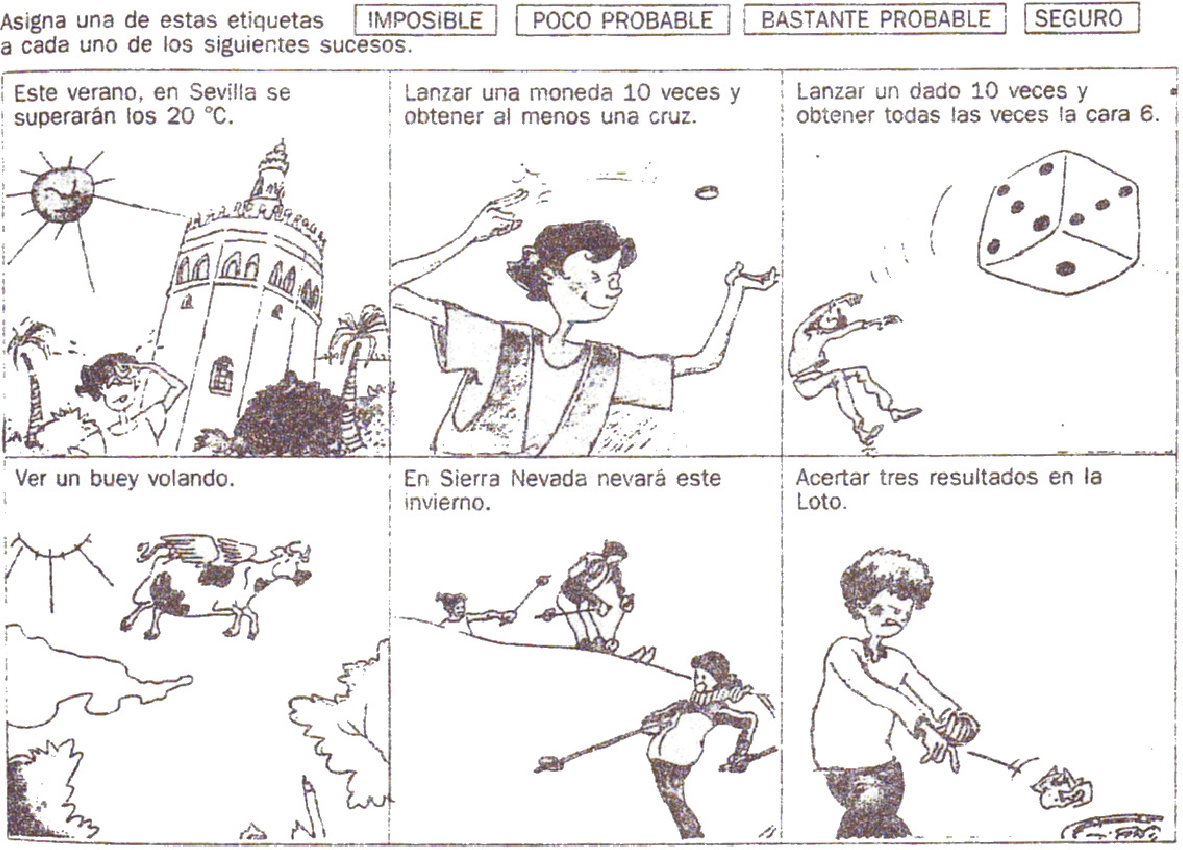
\includegraphics[width=16cm]{BD}
            \end{center}
            \begin{itemize}
               \item Vignette 1 : \pointilles
               \item Vignette 2 : \pointilles
               \item Vignette 3 : \pointilles
               \item Vignette 4 : \pointilles
               \item Vignette 5 : \pointilles
               \item Vignette 6 : \pointilles
            \end{itemize}

         \AApartie{Exploitation}
            Classer ces vignettes sur l'échelle ci-dessous en indiquant le numéro de la vignette en dessous de l'échelle.
            \begin{center}
               \begin{pspicture}(0,-1)(12,0.5)
                  \psline{->}(0,0)(12,0)
                  \footnotesize
                  \rput(0,0.3){imposible}
                  \rput(4,0.3){poco probable}
                  \rput(8,0.3){bastante probable}
                  \rput(12,0.3){seguro}
               \end{pspicture}
            \end{center}

   \end{AActivite}

   \vfill\hfill{\it\footnotesize Source : \href{https://publimath.univ-irem.fr/numerisation/RO/IRO09001/IRO09001.pdf}{\og Une initiation aux probabilités par le jeu \fg}, IREM de Rouen.}

\end{Maquette}


%%%Trace écrite %%%
\begin{Maquette}[Cours]{Theme={Trace écrite},Couleur={0.4[SteelBlue,Black]}}

   %%%1
   \section{Vocabulaire des probabilités}

      \begin{definition*}{}
         On appelle \textbf{expérience aléatoire} une expérience dont on ne peut pas prévoir le résultat de façon certaine.
      \end{definition*}

      \begin{exemple*}{}
         Lancer une pièce de monnaie est une expérience aléatoire dont le résultat est soit \og pile \fg, soit \og face \fg.
      \end{exemple*}

      \begin{definition*}{}
         \begin{itemize}
            \item Chaque résultat possible et prévisible d'une expérience aléatoire est appelé une \textbf{issue}.
            \item L'ensemble formé par les issues est appelé \textbf{univers}, souvent noté $\Omega$.
            \item Un \textbf{événement} de l'expérience aléatoire est une partie quelconque de l'univers.
         \end{itemize}
      \end{definition*}

      \begin{exemple*}{}
         \begin{itemize}
            \item Lancer d'une pièce de monnaie : $\Omega =\{$~pile~;~face~$\}$.
            \item Lancer d'un dé à six faces : $\Omega =\{~1~;~2~;~3~;~4~;~5~;~6~\}$.
            \item \og Obtenir un numéro pair \fg{} est un événement que l'on peut noter $A=\{~2~;~4~;~6~\}$.
         \end{itemize}
      \end{exemple*}


   \section{Calcul de probabilités} %%%

      La probabilité $P$ d'un événement est \og la chance \fg{} qu'il se produise.

      \begin{definition*}{}
         On dit qu'il y a \textbf{équiprobabilité} lorsque toutes les issues ont la même probabilité ; \par \smallskip
         dans ce cas, on a $P=\dfrac{\textrm{nombre d'issues favorables}}{\textrm{nombre de cas possibles}}$.
      \end{definition*}

      Remarque : dans un exercice, pour signifier que l'on est dans une situation d'équiprobabilité, on a des expressions du type : \og on lance un dé \textbf{non pipé} \fg ; \og dans une urne, les boules sont \textbf{indiscernables} au toucher \fg ; \og on rencontre \textbf{au hasard} une personne parmi\dots \fg.

      \begin{exemple*}{}
         On tire une carte dans un jeu non truqué de 52 cartes. Quelle est la probabilité d'obtenir une tête ? \par
         Le jeu est non truqué, il y a donc équiprobabilité. Les issues possibles sont le valet, la dame et le roi de pique, de carreau, de trèfle et de c\oe ur ce qui fait $4\times3$ cartes donc, $P =\dfrac{12}{52}$.
      \end{exemple*}

      \begin{propriete*}{}
         Un probabilité est toujours comprise entre 0 et 1. Si elle est égale à 0, on dit que l'événement est {\bf impossible} et si elle est égale à 1, l'événement est {\bf certain}.
      \end{propriete*}

      \begin{exemple*}{}
         On lance un dé classique équilibré à six faces. Quelle est la probabilité d'obtenir un 9 ? d'obtenir un nombre entier ? \par
         Nous sommes dans une situation d'équiprobabilité.
         \begin{itemize} 
            \item On ne peut pas obtenir un 9 avec un dé à 6 faces donc, $P =\dfrac06 =0$.
            \item Tous les nombres obtenus sont entiers donc, $P =\dfrac66 =1$.
         \end{itemize}
      \end{exemple*}

\end{Maquette}


%%% Exercices %%%
\begin{Maquette}[Fiche,CorrigeFin,Colonnes=2]{}
   
   \begin{multicols}{2}

      \begin{exercice}[SLF] %1
         Pour chacun des événements suivants, indiquer s'il relève du hasard et si oui, le placer sur l'échelle ci-dessous.
         \begin{center}
            \begin{pspicture}(0,-0.5)(7.9,0.5)
               \psline{->}(0.3,0)(7.7,0)
               \rput(4,0){|}
               \footnotesize
               \rput{90}(0.1,-0.2){impossible}
               \rput{90}(7.9,0){certain}
               \rput(1.2,0.3){improbable}
               \rput(3,0.3){peu probable}
               \rput(4.8,0.3){probable}
               \rput(6.5,0.3){très probable}
            \end{pspicture}
         \end{center}
         \begin{enumerate}
            \item Obtenir pile au jeu de pile ou face \pointilles
            \item La fête nationale aura lieu le 14 juillet \pointilles
            \item Un élève aura des baskets demain \pointilles
            \item Obtenir 6 avec un dé à six faces \pointilles
            \item Trouver la bonne combinaison au loto \pointilles
            \item Demain il fera beau \pointilles
         \end{enumerate}
      \end{exercice}
      
      \begin{Solution}
         \begin{enumerate}
            \item Obtenir pile au jeu de pile ou face : \cor{hasard}.
            \item La fête nationale aura lieu le 14 juillet.
            \item Un élève aura des baskets demain : \cor{hasard}.
            \item Obtenir 6 avec un dé à six faces : \cor{hasard}.
            \item Trouver la bonne combinaison au loto : \cor{hasard}.
            \item Demain il fera beau : \cor{hasard}.
         \end{enumerate}
         \begin{pspicture}(0,-0.9)(8,0.9)
            \psline{->}(0.3,0)(7.7,0)
            \rput(4,0){|}
            \footnotesize
            \rput{90}(0.1,0){impossible}
            \rput{90}(7.9,0){certain}
            \rput(1.2,0.3){improbable}
            \rput(3,0.3){peu probable}
            \rput(4.8,0.3){probable}
            \rput(6.5,0.3){très probable}
            \rput(5,-0.4){\cor{1}}
            \rput(7.7,-0.4){\cor{2}}
            \rput(6,-0.4){\cor{3}}
            \rput(3,-0.4){\cor{4}}
            \rput(1,-0.4){\cor{5}}
            \rput(3.9,-0.4){\cor{6}}
         \end{pspicture}
      \end{Solution}
      
      
      \begin{exercice}[SLF] %2
         Une roue de loterie est partagée en huit secteurs identiques numérotés de 1 à 8. Calculer la probabilité de chaque événement et les placer sur l'échelle.
         \begin{center}
            \begin{pspicture}(0,-0.5)(7.9,0.5)
               \psline{->}(0.3,0)(7.7,0)
               \rput(4,0){|}
               \footnotesize
               \rput{90}(0.1,-0.2){impossible}
               \rput{90}(7.9,0){certain}
               \rput(1.2,0.3){improbable}
               \rput(3,0.3){peu probable}
               \rput(4.8,0.3){probable}
               \rput(6.5,0.3){très probable}
            \end{pspicture}
         \end{center}
         \begin{enumerate}
            \item \og Obtenir 2 : \pointilles
            \item \og Obtenir un multiple de 2 : \pointilles
            \item \og Obtenir un nombre supérieur à 4 : \pointilles
            \item \og Obtenir un nombre positif : \pointilles
            \item \og Obtenir un nombre impair : \pointilles
            \item \og Obtenir un multiple de 13 : \pointilles
         \end{enumerate}
      \end{exercice}
      
      \begin{Solution}
         \begin{enumerate}
            \item Obtenir 2 : \cor{$P =1/8$}
            \item Obtenir un multiple de 2 : \cor{$P =4/8$}
            \item Obtenir un nombre supérieur à 5 : \cor{$P =3/8$}
            \item Obtenir un nombre positif : \cor{$P =8/8 =1$}
            \item Obtenir un nombre impair : \cor{$P =4/8$}
            \item Obtenir un multiple de 13 : \cor{$P =0/8 =0$}
         \end{enumerate}
         \begin{pspicture}(0,-1)(8,0.9)
            \psline{->}(0.3,0)(7.7,0)
            \rput(4,0){|}
            \footnotesize
            \rput{90}(0.1,0){impossible}
            \rput{90}(7.9,0){certain}
            \rput(1.2,0.3){improbable}
            \rput(3,0.3){peu probable}
            \rput(4.8,0.3){probable}
            \rput(6.5,0.3){très probable}
            \rput(3,-0.4){\cor{1}}
            \rput(5,-0.4){\cor{2 et 5}}
            \rput(4,-0.4){\cor{3}}
            \rput(7.5,-0.4){\cor{4}}
            \rput(0.5,-0.4){\cor{6}}
         \end{pspicture}
      \end{Solution}

       
      \begin{exercice} %3
         Roudayna tire une carte dans un jeu ordinaire de cinquante-deux cartes.
         \begin{enumerate}
            \item Donner les probabilités qu'elle obtienne les événements suivants : \og Obtenir un carreau \fg ; \og Obtenir un valet \fg{} et \og Obtenir un valet de carreau \fg.
            \item Calculer la probabilité de ne pas obtenir de carreau.
         \end{enumerate}
      \end{exercice}
      
      \begin{Solution}
         \begin{enumerate}
            \item Obtenir un carreau : $\cor{P =\dfrac{13}{52}}$. \par
               Obtenir un valet : $\cor{P =\dfrac{4}{52}}$. \par
               Obtenir un valet de carreau  : $\cor{P =\dfrac{1}{52}}$. \smallskip
            \item La probabilité de ne pas obtenir de carreau s'obtient en calculant la probabilité d'obtenir un c\oe ur, un pique ou un trèfle, ce qui fait au total $3\times13$ carte, soit 39 cartes. \cor{$P =\dfrac{39}{52}$}.
         \end{enumerate}      
      \end{Solution}
      
      
      \begin{exercice} %4
         On dispose d’un dé à six faces numérotées de 1 à 6 et d’un dé à quatre faces avec des sommets numérotés de 1 à 4, parfaitement équilibrés. On lance les deux dés.
         \begin{enumerate}
            \item Avec quel dé la probabilité d’obtenir un 3 est-elle la plus grande ?
            \item Avec quel dé la probabilité d’obtenir un multiple de 3 est-elle la plus grande ?
         \end{enumerate}
      \end{exercice}
      
      \begin{Solution}
         \begin{enumerate}
            \item Dé à six faces : $P =\dfrac16$ (obtenir 3) ; \par
               dé à quatre faces : $P =\dfrac14$ (obtenir 3). \par \smallskip
               C'est avec le \cor{dé à quatre faces} que la probabilité d'obtenir un 3 est la plus grande.
            \item Dé à six faces : $ P =\dfrac26$ (obtenir 3 ou 6) ; \par
               dé à quatre faces : $P =\dfrac14$ (obtenir 3). \par  \smallskip
               C'est avec le \cor{dé à six faces} que la probabilité d'obtenir un multiple de 3 est la plus grande.
         \end{enumerate}
      \end{Solution}
      
      
      \begin{exercice}[Dur] %5
         On écrit sur les faces d’un dé équilibré à six faces, chacune des lettres du mot : NOTOUS. On lance le dé et on regarde la lettre inscrite sur la face supérieure.
         \begin{enumerate}
            \item Quelles sont les issues de cette expérience ?
            \item Déterminer la probabilité des évènements suivants :
            \begin{enumerate}
               \item $E_1$ : \og On obtient la lettre O. \fg
               \item $E_2$ : \og On obtient une consonne. \fg
               \item $E_3$ : \og On obtient une lettre du mot KIWI. \fg
               \item $E_4$ : \og On obtient une lettre du mot CAGOUS. \fg
            \end{enumerate}
            \item Graduer un axe et y placer les probabilités des évènements précédents.
         \end{enumerate}
      \end{exercice}
      
      \begin{Solution}
         \begin{enumerate}
            \item Les issues possibles sont les lettres \cor{N, O, T, U, S}
            \item
               \begin{enumerate}
                  \item $E_1=\{\text{O}\}$ (lettre double) donc, \cor{$P(E_1) =\dfrac26$}
                  \item  $E_2=\{\text{N, T, S}\}$ donc, \cor{$P(E_2) =\dfrac36$}
                  \item  $E_3=\{\varnothing\}$ donc, \cor{$P(E_3) =\dfrac06 =0$}
                  \item  $E_4=\{\text{O, U, S}\}$ donc, \cor{$P(E_4) =\dfrac46$}
               \end{enumerate}
            \item Axe de graduation : \par
               \begin{pspicture}(0,-0.5)(8,0.9)
                  \psline{->}(0.3,0)(7.7,0)
                  \rput(4,0){|}
                  \footnotesize
                  \rput{90}(0.1,0){impossible}
                  \rput{90}(7.9,0){certain}
                  \rput(1.2,0.3){improbable}
                  \rput(3,0.3){peu probable}
                  \rput(4.8,0.3){probable}
                  \rput(6.5,0.3){très probable}
                  \rput(3.5,-0.5){\cor{$E_1$}}
                  \rput(4.5,-0.5){\cor{$E_2$}}
                  \rput(0.5,-0.5){\cor{$E_3$}}
                  \rput(5.5,-0.5){\cor{$E_4$}}
               \end{pspicture}
         \end{enumerate}
      \end{Solution}
      
      
      \begin{exercice} %6
         Trois personnes, Ali, Ben et Charles, ont chacune un sac contenant des billes. Chacune tire au hasard une bille de son sac dont le contenu est le suivant : \par \smallskip
            {\hautab{1.3}
            \begin{tabular}{|*{3}{C{2.2}|}}
               \hline
               Sac d'Ali & Sac de Ben & Sac de Charles \\
               \hline
               10 billes rouges & 97 billes rouges & 5 billes rouges \\
               30 billes noires & 3 billes noires & \\
               \hline
            \end{tabular}} \par \smallskip
         Laquelle de ces trois personnes a-t-elle la plus grande probabilité de tirer une bille rouge ? Justifier.
      \end{exercice}
      
      \begin{Solution}
         Probabilité de tirer une bille rouge :
         \begin{itemize}
            \item Pour Ali : $P =\dfrac{10}{40} =0,25$. \smallskip
            \item Pour Ben : $P =\dfrac{97}{100} =0,97$. \smallskip
            \item Pour Charles : $P =\dfrac{5}{5} =1$. \smallskip
         \end{itemize}
         \cor{Charles a la plus grande probabilité d'obtenir une bille rouge}, ce qui est logique puisqu'il n'a QUE des billes rouges.
      \end{Solution}
      
      
      \begin{exercice}[Dur] %7
         Dans les sac suivants, il y a déjà des billes noires et des billes rouges. \par
         Est-il possible d’ajouter un certain nombre (de ton choix) de billes bleues, de façon à satisfaire les indications données en dessous de chaque sac ? \par \smallskip
         \begin{minipage}{2.5cm} %cas 1
            \sac{\psdots[linewidth=1.5mm](0.5,0)(1,0)(1.25,0.5)(1,1)
               \psdots[linewidth=1.5mm,linecolor=red](0.25,0.5)(0.75,0.5)(0.5,1)}
         \end{minipage}
         \begin{minipage}{5.3cm}
            {\bf Cas n°1 :} \par
            La probabilité d'extraire \par
            une bille bleue est $\dfrac{5}{12}$.
         \end{minipage} \\
         \begin{minipage}{2.5cm} %cas 2
            \sac{\psdots[linewidth=1.5mm](0.25,0.5)(1,0)(1.25,0.5)
               \psdots[linewidth=1.5mm,linecolor=red](0.5,0)(0.75,0.5)(1,1)}
         \end{minipage}
         \begin{minipage}{5.3cm}
            {\bf Cas n°2 :} \par
            La probabilité d'extraire \par
            une bille bleue est $\dfrac{2}{5}$.
         \end{minipage} \\
         \begin{minipage}{2.5cm} %cas 3
            \sac{\psdots[linewidth=1.5mm](0.5,0)(0.75,0.5)
               \psdots[linewidth=1.5mm,linecolor=red](0.25,0.5)(0.5,1)(1,0)}
         \end{minipage}
         \begin{minipage}{5.3cm}
            {\bf Cas n°3 :} \par
            La probabilité d'extraire \par
            une bille rouge ou bleue est $\dfrac{3}{4}$.
         \end{minipage}
      \end{exercice}
      
      \begin{Solution}
         \begin{itemize}
            \item Cas n°1 : une probabilité de $\dfrac{5}{12}$ signifie que, pour 12 billes au total, 5 sont bleues. \par
               On a 7 billes, \cor{si on ajoute 5 billes bleue}, on aura bien une chance d'obtenir une bille bleue de $\dfrac{5}{12}$.
            \item Cas n°2 : une probabilité de $\dfrac{2}{5}$ signifie que, pour 5 billes au total, 2 sont bleues, ou encore que pour 10 billes, 4 sont bleues. \par
               On a 6 billes, \cor{si on ajoute 4 billes bleues}, on aura bien une chance d'obtenir une bille bleue de $\dfrac{2}{5}$.
            \item Cas n°3 : une probabilité de $\dfrac{3}{4}$ signifie que, pour 4 billes au total, 3 sont rouges ou bleues, ou encore que pour 8 billes, 6 sont rouges ou bleues. \par
               On a 3 billes rouges et 2 billes noires, \cor{si on ajoute 3 billes bleues}, on aura bien une chance d'obtenir une bille rouge ou bleue de $\dfrac{3}{4}$.
         \end{itemize}
      \end{Solution}

   \end{multicols}

\end{Maquette}


%%% Récré %%%
\begin{Maquette}[Cours]{Theme={Activité récréative},Couleur={IndianRed}}
    
   \ARtitre{Vers la loi des grands nombres\dots}

      {\hautab{2}
      \begin{enumerate}
         \item Compléter le tableau suivant : \par
            \begin{tabular}{|c|*{6}{C{1}|}}
               \hline
               Numéro sur la face visible du dé & 1 & 2 & 3 & 4 & 5 & 6 \\
               \hline
               Probabilité d'obtenir cette face (fraction) & & & & & & \\
               \hline
               Probabilité d'obtenir cette face (décimal) & & & & & & \\
               \hline
            \end{tabular} \par \bigskip
            Que remarque-t-on ? \pointilles

         \vfill

         {\bf Le travail s'effectue maintenant en binôme, vous avez à votre disposition un dé classique à six faces.}

         \vfill

         \item Lancer 10 fois le dé et noter les résultats obtenus dans le tableau suivant : \par \smallskip
            \begin{tabular}{|c|*{6}{C{1}|}}
               \hline
               Numéro sur la face visible du dé & 1 & 2 & 3 & 4 & 5 & 6 \\
               \hline
               Nombre de fois où cette face est obtenue & & & & & & \\
               \hline
               Probabilité d'obtenir cette face (fraction) & & & & & & \\
               \hline
               Probabilité d'obtenir cette face (décimal) & & & & & & \\
               \hline
            \end{tabular} \par \bigskip
            Que remarque-t-on ? \pointilles

         \vfill

         \item Lancer 100 fois le dé et noter les résultats obtenus dans le tableau suivant : \par \smallskip
            \begin{tabular}{|c|*{6}{C{1}|}}
               \hline
               Numéro sur la face visible du dé & 1 & 2 & 3 & 4 & 5 & 6 \\
               \hline
               Nombre de fois où cette face est obtenue & & & & & & \\
               \hline
               Probabilité d'obtenir cette face (fraction) & & & & & & \\
               \hline
               Probabilité d'obtenir cette face (décimal) & & & & & & \\
               \hline
            \end{tabular} \par \bigskip
            Que remarque-t-on ? \pointilles
         
         \vfill

         \item Répertorier les résultats de la classe entière et noter les résultats obtenus dans le tableau suivant : \\ [1mm]
            \begin{tabular}{|c|*{6}{C{1}|}}
               \hline
               Numéro sur la face visible du dé & 1 & 2 & 3 & 4 & 5 & 6 \\
               \hline
               Nombre de fois où cette face est obtenue & & & & & & \\
               \hline
               Probabilité d'obtenir cette face (fraction) & & & & & & \\
               \hline
               Probabilité d'obtenir cette face (décimal) & & & & & & \\
               \hline
            \end{tabular} \par \bigskip
            Que remarque-t-on ? \pointilles
      \end{enumerate}}

   
\end{Maquette}
    \pagebreak
    \graphicspath{{../../S13_Expressions_litterales/Images/}}

\themeN
\chapter{Expressions littérales}
\label{S13}

\programme%
   {\item Notion d'inconnue.}
   {\item Utiliser le calcul littéral pour traduire une propriété générale, pour démontrer un résultat général, pour valider ou réfuter une conjecture, pour modéliser une situation.}

\vfill

\begin{debat}{Débat : petits contes mathématiques}
   Les vidéos des {\bf Petits contes mathématiques} ont été créés par {\it Universciences} : c'est une série pédagogique qui retrace l'histoire des maths à travers la découverte d'une notion, d'une formule, d'une conjecture ou d'une équation. Le récit est rythmé par des illustrations animées et la légèreté du ton dédramatise le sujet pour tous ceux qui ne seraient pas des \og matheux \fg.
   \tcblower
      \begin{pspicture}(0,0)(5,3)
         \rput{10}(1,1){\huge $x$}
         \rput{20}(3.5,2.25){\huge $y$}
         \rput{-10}(3,0.5){\huge $z$}
         \rput(0.5,2.5){\huge $+$}
         \rput(2,1.5){\huge $\times$}
         \rput(4.5,2){\huge $()$}
         \rput(5,0.75){\huge $-$}
         \rput(2,3){\huge $\div$}
         \rput{-20}(5,3){\huge $t$}
      \end{pspicture}
\end{debat}

\hfill {\gray Vidéo : \href{https://leblob.fr/fondamental/le-x}{\bf Le $x$}, site Internet {\it Le blob}, épisode de la série {\it Petits contes mathématiques}.}


%%% Approche %%%
\begin{Maquette}[Cours]{Theme={Activité d'approche},Couleur={SteelBlue}}

   \AAtitre{Des variables aux inconnues}

      {\it Objectifs : voir l'effet des variables dans un programme de calcul créé avec Scratch ; produire une expression littérale.}

      \begin{AActivite}

         On considère le programme de calcul ci-dessous dans lequel $x$, Etape 1, Etape 2 et Résultat sont quatre variables.
         \begin{center}
            \begin{Scratch}[Echelle=0.9]
               Place Drapeau ;
               Place Demander("Choisis un nombre");
               Place MettreVar("x",OvalCap("réponse"));
               Place DireT("Je multiplie le nombre par 6.","2");
               Place MettreVar("Etape 1",OpMul("6",OvalVar("x")));
               Place DireT("J'ajoute 10 au résultat.","2");
               Place MettreVar("Etape 2",OpAdd(OvalVar("Etape 1"),"10"));
               Place DireT("Je divise le résultat par 2.","2");
               Place MettreVar("Résultat",OpDiv(OvalVar("Etape 2"),"2"));
               Place Dire(OpRegrouper("J'obtiens finalement",OvalVar("Résultat")));
            \end{Scratch}
         \end{center}
         \begin{enumerate}
            \item Yasmina a fait fonctionner ce programme en choisissant le nombre 5.\par
            Vérifier que ce qui est dit à la fin est : \og J’obtiens finalement 20 \fg. Pour cela, remplir le diagramme suivant : \par
               \begin{pspicture}(-3,-0.1)(8,1.8)
                  \psframe(0,0.5)(1,1.5)
                  \rput(0.5,0){$x$}
                  \psline[arrowsize=2mm]{->}(1.1,1)(2.4,1)
                  \psframe(2.5,0.5)(3.5,1.5)
                  \rput(3,0){étape 1}
                  \psline[arrowsize=2mm]{->}(3.6,1)(4.9,1)
                  \psframe(5,0.5)(6,1.5)
                  \rput(5.5,0){étape 2}
                  \psline[arrowsize=2mm]{->}(6.1,1)(7.4,1)
                  \psframe(7.5,0.5)(8.5,1.5)
                  \rput(8,0){résultat}
               \end{pspicture}         
            \item Que dit le programme si Maissa le fait fonctionner en choisissant au départ le nombre 7 ? \par
               \begin{pspicture}(-3,-0.1)(8,1.8)
                  \psframe(0,0.5)(1,1.5)
                  \rput(0.5,0){$x$}
                  \psline[arrowsize=2mm]{->}(1.1,1)(2.4,1)
                  \psframe(2.5,0.5)(3.5,1.5)
                  \rput(3,0){étape 1}
                  \psline[arrowsize=2mm]{->}(3.6,1)(4.9,1)
                  \psframe(5,0.5)(6,1.5)
                  \rput(5.5,0){étape 2}
                  \psline[arrowsize=2mm]{->}(6.1,1)(7.4,1)
                  \psframe(7.5,0.5)(8.5,1.5)
                  \rput(8,0){résultat}
               \end{pspicture}         
            \item Firdaws fait fonctionner le programme, et ce qui est dit à la fin est : \og J’obtiens finalement 8 \fg. Quel nombre a-t-elle choisi au départ ? \par
               \begin{pspicture}(-3,-0.1)(8,1.2)
                  \psframe(0,0.5)(1,1.5)
                  \rput(0.5,0){$x$}
                  \psline[arrowsize=2mm]{<-}(1.1,1)(2.4,1)
                  \psframe(2.5,0.5)(3.5,1.5)
                  \rput(3,0){étape 1}
                  \psline[arrowsize=2mm]{<-}(3.6,1)(4.9,1)
                  \psframe(5,0.5)(6,1.5)
                  \rput(5.5,0){étape 2}
                  \psline[arrowsize=2mm]{<-}(6.1,1)(7.4,1)
                  \psframe(7.5,0.5)(8.5,1.5)
                  \rput(8,0){résultat}
               \end{pspicture} 
            \item Si l’on appelle $x$ le nombre choisi au départ, écrire en fonction de $x$ l’expression obtenue à la fin du programme. \par
               \begin{pspicture}(-3,0.1)(8,1.8)
                  \psframe(0,0.5)(1,1.5)
                  \rput(0.5,1){$x$}
                  \psline[arrowsize=2mm]{->}(1.1,1)(2.4,1)
                  \psframe(2.5,0.5)(4,1.5)
                  \rput(3.25,0){étape 1}
                  \psline[arrowsize=2mm]{->}(4.1,1)(5.4,1)
                  \psframe(5.5,0.5)(7.5,1.5)
                  \rput(6.5,0){étape 2}
                  \psline[arrowsize=2mm]{->}(7.6,1)(8.9,1)
                  \psframe(9,0.5)(12,1.5)
                  \rput(10.5,0){résultat}
               \end{pspicture} 
         \end{enumerate}

      \end{AActivite}

      \vfill\hfill{\it\footnotesize Source : cette activité est une adaptation du DNB 2017 de Pondichery.}

\end{Maquette}


%%%Trace écrite %%%
\begin{Maquette}[Cours]{Theme={Trace écrite},Couleur={0.4[SteelBlue,Black]}}

   %%%1
   \section{Expressions littérales}
   
      \begin{definition*}{}
         Une {\bf expression littérale} est une succession d'opérations où apparaissent des lettres représentant des nombres. \par
         On parle aussi d'{\bf expression algébrique}.
      \end{definition*}
      
      \begin{exemple*}{}
         $4\times x+3$ \; ; \; $2\times a-89$ \; ; \; $y-3\times z+t-4$.
      \end{exemple*}
   
   
   %%%2
   \section{Produire une expression littérale}
   
      On utilise notamment des expressions littérales pour produire des  formules générales, qui pourront être utilisées quelle que soit la valeur des variables.
      
      \begin{exemple*}{}
         \begin{itemize}
            \item Matéo a quatre ans de plus que Noé. \par
               En appelant \og $x$ \fg{} l'âge de Noé, l'âge de Matéo peut s'écrire \og $x+4$ \fg.
            \item Un rectangle a pour largeur $\ell$ et pour longueur $L$. \par
               Son périmètre peut s'exprimer ainsi : $\mathcal{P} =2\times(\ell+L)$. \par
               Son aire peut s'exprimer ainsi : $\mathcal{A} =\ell\times L$. \par
         \end{itemize}
      \end{exemple*}
      
      Remarque : la circonférence d'un disque s'écrit $2\pi R$ où :
         \begin{itemize}
            \item $\pi$ est une lettre grecque qui désigne le nombre 3,14\dots, qui est fixe ;
            \item $R$ est une lettre qui désigne le rayon du disque, ce nombre est variable et dépend du disque.
         \end{itemize}
   
   
   %%%%3
   \section{Simplifier d'une expression littérale}
   
   Pour simplifier une expression littérale, on peut supprimer le signe \og $\times$ \fg{} devant une lettre, une parenthèse ou entre deux lettres. 
   
   \begin{propriete*}{}
      \begin{itemize}
         \item On utilise la notation $2a$ pour $a+a$ ou $a\times2$ ou encore $2\times a$. On dit \og deux a \fg.
         \item On utilise la notation $ab$ pour $a\times b$. On dit \og ab \fg.
         \item On utilise la notation $a^2$ pour $a\times a$. On dit \og a au carré \fg.
         \item On utilise la notation $a^3$ pour $a\times a\times a$. On dit \og a au cube \fg.
      \end{itemize}
   \end{propriete*}

   
   On écrit une expression comportant un nombre et une \og lettre \fg{} avec le nombre précédé de la \og lettre \fg.
   
   \begin{exemple*}{}
      Simplifier les expressions : \par
      $A =5\times y-2\times x =5y-2x$ \par
      $B =x\times x \times x + 7\times y\times y =x^3+7y^2$. \par
      $C =x\times3 =3x$, est préférable à $C=x3$. \par
         Par commutativité de la multiplication, $x\times3 =3\times x =3x$.
   \end{exemple*}

\end{Maquette}


%%% Exercices %%%
\begin{Maquette}[Fiche,CorrigeFin,Colonnes=2]{}

   \begin{multicols}{2}

      \begin{exercice} %1
         Si $x$ représente un nombre, comment peut-on écrire les expressions suivantes :
         \begin{enumerate}
            \item Le double de $x$.
            \item Le tiers de $x$.
            \item La somme de $x$ et de 13.
            \item La différence de $x$ et de 7.
            \item Le triple de la somme de 2 et de $x$.
            \item Le tiers de la différence de 16 et $x$.
         \end{enumerate}
      \end{exercice}
         
      \begin{Solution}
         \begin{enumerate}
            \item $2\times x =\cor{2x}$ \smallskip
            \item $\dfrac13\times x =\cor{\dfrac13x =\dfrac{x}{3}}$ \smallskip
            \item $\cor{x+13}$
            \item $\cor{x-7}$
            \item $3\times(2+x) =\cor{3(2+x)}$ \smallskip
            \item $\dfrac13\times(16-x) =\cor{\dfrac13(16-x) =\dfrac{16-x}{3}}$
         \end{enumerate}
      \end{Solution}
      

      \begin{exercice} %2
         Si on note $z$ l'âge en années de Zahra aujourd’hui, comment peut-on noter :
         \begin{enumerate}
            \item L'âge qu'elle aura dans deux ans ?
            \item Le triple de l'âge qu'elle avait il y a quatre ans ?
            \item La moitié de l'âge qu'elle aura dans cinq ans ?
            \item Son année de naissance si on est en 2024 ?
         \end{enumerate}
      \end{exercice}
      
      \begin{Solution}
         \begin{enumerate}
            \item $\cor{z+2}$
            \item $\cor{3(z-4)}$
            \item $\cor{\dfrac12(z+5) =\dfrac{z+5}{2}}$ \smallskip
            \item $\cor{2024-z}$
         \end{enumerate}
      \end{Solution}
      
      
      \begin{exercice}[SLF] %3
         Recopier les expressions suivantes en supprimant les signes $\times$ s'ils ne sont pas nécessaires.
         \begin{itemize}
            \item $A =9\times n =\pointilles$ \medskip
            \item $B =x\times3 =\pointilles$ \medskip
            \item $C =12\times(a-3) =\pointilles$ \medskip
            \item $D =2\times a(2\times8) =\pointilles$ \medskip
            \item $E =n\times x =\pointilles$ \medskip
            \item $F =2\times\pi\times R =\pointilles$ \medskip
         \end{itemize}
      \end{exercice}
      
      \begin{Solution}
         \begin{itemize}
            \item $A =9\times n =\cor{9n}$
            \item $B =x\times3 =\cor{3x}$
            \item $C =12\times(a-3) =\cor{12(a-3)}$
            \item $D =2\times a(2\times8) =2\times16a =\cor{32a}$
            \item $E =n\times x =\cor{nx}$
            \item $F =2\times\pi\times R =\cor{2\pi R}$
         \end{itemize}
      \end{Solution}

      
      \begin{exercice}[SLF] %4
         Simplifier les expressions suivantes :
         \begin{itemize}
            \item $A =a\times a =\pointilles$ \medskip
            \item $B =b\times b\times b =\pointilles$ \medskip
            \item $C =c\times c\times3 =\pointilles$ \medskip
            \item $D =9+d\times d\times d =\pointilles$ \medskip
            \item $E =a\times a\times b\times3 =\pointilles$ \medskip
            \item $F =x\times x\times x-2\times y\times y =\pointilles$ \medskip
            \item $G =(a+b)\times(a+b) =\pointilles$ \medskip
            \item $H =(x+y)(x+y)(x+y) =\pointilles$ \medskip
         \end{itemize}
      \end{exercice}
      
      \begin{Solution}
         \begin{itemize}
            \item $A =a\times a =\cor{a^2}$
            \item $B =b\times b\times b =\cor{b^3}$
            \item $C =c\times c\times3 =\cor{3c^2}$
            \item $D =9+d\times d\times d =\cor{9+d^3}$
            \item $E =a\times a\times b\times3 =\cor{3a^2b}$
            \item $F =x\times x\times x-2\times y\times y =\cor{x^3-2y^2}$
            \item $G =(a+b)\times(a+b) =\cor{(a+b)^2}$
            \item $H =(x+y)(x+y)(x+y) =\cor{(x+y)^3}$ \medskip
         \end{itemize}
      \end{Solution}
      
      
      \begin{exercice}[SLF] %5
         Dire si chaque affirmation est vraie ou fausse. \par \medskip
         \QCM[VF,Stretch=1.8,Largeur=1cm,NomV=vrai,NomF=Faux]{%
            $x\times x = 2x$&2,%
            $x+x = 2x$&1,%
            $x\times x =x^{2}$&1,%
            $x+x =x^{2}$&2,%
            $x+2 =2x$&2,%
            $x+2=x^{2}$&2,}
      \end{exercice}
      
      \begin{Solution}
         \QCM[VF,Stretch=1.8,Largeur=1cm,NomV=vrai,NomF=Faux,Solution]{%
            $x\times x = 2x$&2,%
            $x+x = 2x$&1,%
            $x\times x =x^{2}$&1,%
            $x+x =x^{2}$&2,%
            $x+2 =2x$&2,%
            $x+2=x^{2}$&2,}
      \end{Solution}
      
      
      \begin{exercice} %6
         Voici un programme :
         \begin{center}
            \ProgCalcul[Enonce,Largeur=4.5cm]{
               Choisis un nombre,
               Retire-lui 5,
               Multiplie le résultat par 3}
         \end{center}
         \begin{enumerate}
            \item Faire fonctionner le programme avec trois nombres de son choix supérieurs ou égaux à 5.
            \item Quel nombre faut-il choisir pour obtenir 6 ?
            \item Soit $x$ le nombre de départ, donner l'expression finale en fonction de $x$.
         \end{enumerate}
      \end{exercice}
      
      \begin{Solution}
         \begin{enumerate}
            \item \ProgCalcul{10,-5 *3}. \par
               Avec 10, on obtient \cor{15} \dots
            \item \ProgCalcul[Direct=false]{7,-5 *3}. \par
               On obtient 6 avec \cor{7}.
            \item \ProgCalcul[SansCalcul]{x,-5 *3,x-5 3(x-5)}. \par
               Ave$x$ on obtient \cor{$3(x-5)$}.
         \end{enumerate}
      \end{Solution}

      
      \begin{exercice}[Dur] %7
         Résoudre les défis suivants.
         \begin{enumerate}
            \item
               \begin{enumerate}
                  \item Choisir deux nombres consécutifs, calculer leur somme et comparer avec les résultats de la classe.
                  \item Quelle conjecture peut-on émettre ?
               \end{enumerate}
            \item On choisit un entier $n$.
               \begin{enumerate}
                  \item Comment s'écrit le nombre suivant $n$ ?
                  \item Donner l'expression de la somme de deux nombres consécutifs en fonction de $n$.
                  \item Démontrer la conjecture.
               \end{enumerate}
            \item Montrer que la somme de trois nombres consécutifs est multiple de 3.
         \end{enumerate}
      \end{exercice}
      
      \begin{Solution}
         \begin{enumerate}
            \item
               \begin{enumerate}
                  \item par exemple, \cor{$16+17 =33$}.
                  \item On peut conjecturer que  \cor{la somme de deux nombres consécutifs est un nombre impair}.
               \end{enumerate}
            \setcounter{enumi}{1}
            \item
               \begin{enumerate}
                  \item Le nombre suivant $n$ s'écrit \cor{$n+1$}.
                  \item $(n)+(n+1) =n+n+1 =\cor{2n+1}$.
                  \item $2n+1$ est un nombre pair ($2n$) auquel on ajoute 1, c'est donc un nombre impair. \\
                     \cor{La conjecture est vraie}.
               \end{enumerate}
            \setcounter{enumi}{2}
            \item Soit $n$ un nombre quelconque, le suivant s'écrit $n+1$ et celui d'après $n+2$. \\
               La somme de trois nombres consécutifs s'écrit alors : \\
               $(n)+(n+1)+(n+2) =n+n+1+n+2 =3n+3$. \\
               $3n+3$ est la somme de deux nombres multiples de 3, \cor{c'est donc un multiple de 3}.
         \end{enumerate}
      \end{Solution}

   \end{multicols}

\end{Maquette}


%%% Récré %%%
\begin{Maquette}[Cours]{Theme={Activité récréative},Couleur={IndianRed}}
    
   \ARtitre{Défis !!!}
   
      \parbox{2cm}{
\includegraphics[width=2cm]{defi} \par \medskip
      \ARpartie{Défi 1}}
      \qquad
      \parbox{14cm}{
         Nihad et Adam ont choisi un nombre (entier positif). \par
         Nihad le multiplie par 5 et ajoute 35. \par
         Adam le multiplie par 2 et ajoute 146. \par
         Ils trouvent le même nombre à la fin. \par
         Quel nombre ont-ils choisi ?}
      
      \vfill
      
      \parbox{2cm}{
\includegraphics[width=2cm]{defi} \par \medskip
      \ARpartie{Défi 2}}
      \qquad
      \parbox{14cm}{
         Avec des petits carrés tous identiques, on construit un pattern selon le modèle évolutif ci-dessous : \par
         {\psset{unit=0.8}
         \begin{pspicture}(-3.5,-4.5)(4,3.75)
            \croix
            \rput(0.5,-2){Rang 1}
         \end{pspicture}
         \begin{pspicture}(-5,-4.5)(5,3.75)
            \croix
            \rput(2,0){\carre}
            \rput(0,2){\carre}
            \rput(-2,0){\carre}
            \rput(0,-2){\carre}
            \rput(0.5,-3){Rang 2}
         \end{pspicture}
         
         \begin{pspicture}(-8,-4.5)(4,1)
            \croix
            \rput(2,0){\carre}
            \rput(3,0){\carre}
            \rput(0,2){\carre}
            \rput(0,3){\carre}
            \rput(-2,0){\carre}
            \rput(-3,0){\carre}
            \rput(0,-2){\carre}
            \rput(0,-3){\carre}
            \rput(0.5,-4){Rang 3}
         \end{pspicture}}
         \begin{enumerate}
            \item Dessiner l’élément du rang suivant et expliquer la règle.
            \item Déterminer le nombre de petits carrés des éléments du rang 5, du rang 10, du rang 17.
            \item Déterminer le nombre de petits carrés de l’élément du rang 100 et donner un moyen de calculer rapidement le nombre de petits carrés d’un élément à n’importe quel rang.
            \item Existe-t-il un élément qui contient 532 petits carrés ? Un élément qui contient 813 petits carrés ?
         \end{enumerate}}
         
   \vfill\hfill {\it\footnotesize Source : \og La résolution de problèmes mathématiques au collège \fg, MENJS, 2021}

\end{Maquette}
    \pagebreak
    \graphicspath{{../../S14_Reconnaitre_des_solides/Images/}}

\themeG
\chapter{Reconnaître des solides}
\label{S14}

\textcolor{red}{\bf Connaissances :}
   \begin{connaissances}
      \item Reconnaître des solides : pavé droit, cube, prisme, cylindre, pyramide, cône et boule.
   \end{connaissances}

\vfill

\begin{debat}{Débat : les solides de Platon}
   Parmi les solides de l'espace, il en est une sorte qui a été étudiée par le philosophe grec {\bf Platon} ($-425;-348$) : les polyèdres réguliers et convexes. Ce dernier associe chacun des quatre éléments physiques avec un solide régulier.
   \begin{itemize}
      \item la {\bf Terre} est associée au {\it cube} : ces petits solides font de la poussière lorsqu'ils sont émiettés et se cassent lorsqu'on s'en saisit ;
      \item l'{\bf air} est associé à l'{\it octaèdre} : ses composants minuscules sont si doux qu'on peut à peine les sentir ;
      \item l'{\bf eau} est associée à l'{\it icosaèdre} : elle s'échappe de la main lorsqu'on la saisit comme si elle était constituée de petites boules minuscules ;
      \item le {\bf feu} est associé au {\it tétraèdre} car la chaleur du feu semble pointue comme un poignard ;
      \item le \textit{dodécaèdre} est mis en correspondance avec le {\bf tout}, parce que c'est le solide qui ressemble le plus à la sphère.
   \end{itemize}
   \tcblower
      \begin{pspicture}(-1,-1)(15,1.8)
         \psset{faceName=\arabic,Frame=false,faceNameFont=\sffamily}
         \rput(0,-0.2){\psTetrahedron}
         \rput(3,0.3){\psHexahedron[psscale=0.8]}
         \rput(6,0.2){\psOctahedron[psscale=1.5,faceNameFont=\scriptsize]}
         \rput(8.8,0.3){\psDodecahedron[psscale=0.8]}
         \rput(11.6,0.2){\psIcosahedron[psscale=0.7]}
      \end{pspicture}
\end{debat}

\hfill {\gray Vidéo : \href{ttps://www.yout-ube.com/watch?v=eDsFmYur9Yo}{\bf Les 5 solides de Platon}, chaîne YouTube {\it Micmaths} de {\it Mickaël Launay}.}


%%% Approche %%%
\begin{Maquette}[Cours]{Theme={Activité d'approche},Couleur={SteelBlue}}

   \AAtitre{Les polydrons}

      {\it Objectifs : construire des solides fermés ; trier des solides selon leur forme.}

      \begin{AActivite}

         Les Polydrons sont des polygones en plastique dur qui peuvent se fixer entre eux à l'aide de charnières. \par
         Ce matériel permet de construire facilement des polyèdres et des patrons. \par
         
         \AApartie{Construction de solides}
            \begin{enumerate}
               \item Citer les différentes formes de Polydrons en précisant leur nature exacte. \par \medskip
                  \pointilles
               \item Construire un premier solide, donner son nom si possible et le dessiner. \par \vskip35mm      
               \item Construire d'autres solides en essayant de varier les formes.
            \end{enumerate} 

         \AApartie{Classement des solides}
            \begin{enumerate}
               \item En regroupant tous les solides de la classe, déterminer un classement commun, discuter des choix.
               \item Citer les classes choisies en expliquant leurs caractéristiques. \par \medskip
                  \pointilles\par \medskip
                  \pointilles \par \medskip
                  \pointilles \par \medskip
                  \pointilles \par \medskip
                  \pointilles \par \medskip
            \end{enumerate}
            \begin{center}
               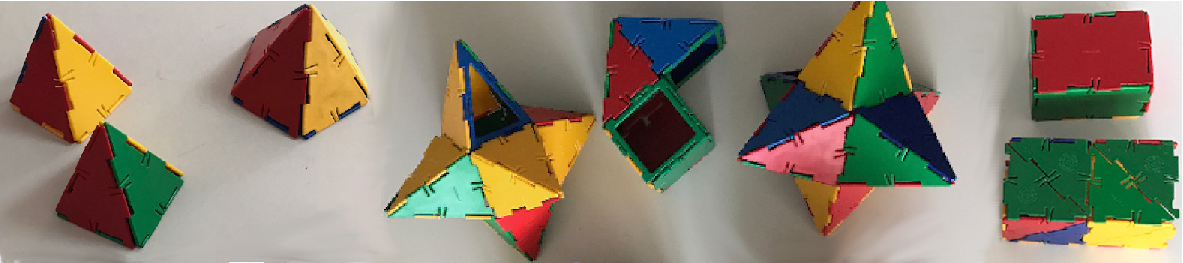
\includegraphics[width=16cm]{polydrons}
            \end{center}

   \end{AActivite}

\end{Maquette}


%%%Trace écrite %%%
\begin{Maquette}[Cours]{Theme={Trace écrite},Couleur={0.4[SteelBlue,Black]}}

   \begin{pspicture}(-0.5,0)(17,24)
      \rput(9.25,10){\ovalnode{A}{\Large Les solides du collège}}
      \rput{90}(0,5){\textcolor{Crimson}{\large Les solides non polyédriques}}
      \rput{90}(0,15){\textcolor{DodgerBlue}{\large Les polyèdres}}
      %prisme
      \psnode(6,12.5){B}{\begin{minipage}{10.5cm}{\bf Prisme} : du grec {\it prismatos}, scié. Deux bases polygonales, des faces latérales qui sont des parallélogrammes, rectangles si le prisme est droit \end{minipage}}
      \rput(5,13.5){{\psset{unit=0.35}\psSolid[object=prisme,h=0.8,action=draw*,linecolor=DodgerBlue]}}
      \rput(8.5,14){
\includegraphics[width=3.25cm]{Cours_Toblerone}}
      \ncline{A}{B}
      \ncput*{\textcolor{DodgerBlue}{prismes}}
      %pavé 
      \psnode(6,16){D}{\begin{minipage}{10.5cm}{\bf Parallélépipède ou pavé} : du grec {\it parallelos}, parallèle et {\it epidon}, surface. Cas particulier du prisme droit lorsque la base est un rectangle \end{minipage}}
      \rput(4.5,17.5){\psSolid[object=parallelepiped,a=0.6,b=0.4,c=0.3,action=draw*,linecolor=DodgerBlue]}
      \rput(8.5,17.5){
\includegraphics[width=2.5cm]{Cours_boite}}
      \psnode(6,13){G}{} 
      %\ncline{G}{D}
      %cube
      \psnode(6,19.5){E}{\begin{minipage}{10.5cm}{\bf Cube} : cas particulier du pavé droit lorsque toutes les faces sont carrées \end{minipage}}
      \rput(4.5,21){\psSolid[object=parallelepiped,a=0.5,action=draw*,RotX=30,linecolor=DodgerBlue]}
      \rput(8.5,21){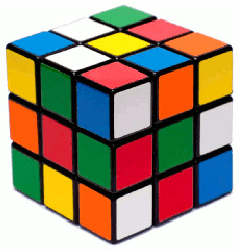
\includegraphics[width=2cm]{Cours_Rubiks}}
      \psnode(6,17){F}{}
      %\ncline{F}{E}
      %Pyramide
      \psnode(14.75,14){C}{\begin{minipage}{4.5cm}{\bf Pyramide} : une base polygonale, un sommet, des faces latérales triangulaires, qui sont isocèles et superposables si la pyramide est régulière \end{minipage}}
      \rput(15,17){\psSolid[object=tetrahedron,r=0.6,action=draw*,RotZ=70,linecolor=DodgerBlue]}
      \rput(14.75,20.5){
\includegraphics[width=4.5cm]{Cours_Kheops}}
      \ncline{A}{C}
      \ncput*{\textcolor{DodgerBlue}{pyramides}}
      %Cylindre
      \psnode(3.75,6.5){D}{\begin{minipage}{4.5cm}{\bf Cylindre} : du grec {\it kulindros}, rouleau. Deux bases en forme de disques, une surface latérale \end{minipage}}
      \rput(4.5,3.5){\psSolid[object=cylindre,h=1,r=0.2,action=draw**,ngrid=8 16,RotX=90,linecolor=Crimson]}
      \rput(3.75,1){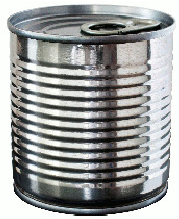
\includegraphics[height=2.75cm]{Cours_conserve}}
      \ncline{A}{D}
      \ncput*{\textcolor{Crimson}{cylindres}}
      %Cône
      \psnode(9.25,6.5){D}{\begin{minipage}{4.5cm}{\bf Cône} : du grec {\it kônos}, pomme de pain. Une base en forme de disque, une surface latérale, un sommet \end{minipage}}
      \rput(9.25,4.85){\psSolid[object=cone,h=0.8,r=0.4,action=draw**,ngrid=8 16,RotX=200,linecolor=Crimson]}
      \rput(10,1){
\includegraphics[height=3cm]{Cours_glace}}
      \ncline{A}{D}
      \ncput*{\textcolor{Crimson}{cônes}}
      %Sphère
      \psnode(14.75,6.5){D}{\begin{minipage}{4.5cm}{La \bf sphère} : du grec {\it sphaîra}, corps rond, est la surface extérieure de la {\bf boule} \end{minipage}}
      \rput(14.75,4.15){\psSolid[object=sphere,r=0.45,ngrid=18 18,linecolor=Crimson]}
      \rput(14.75,1){
\includegraphics[height=2.75cm]{Cours_ballon}}
      \ncline{A}{D}
      \ncput*{\textcolor{Crimson}{boules}}
   \end{pspicture}

\end{Maquette}


%%% Exercices %%%
\begin{Maquette}[Fiche,CorrigeFin,Colonnes=2]{}

   \begin{multicols}{2}

      \begin{exercice} %1
         On considère les catégories de solides suivants que l'on peut trouver dans la vie courante :
         \begin{enumerate}
            \item[A.] Différentes boites parallélépipédiques et cubiques.
            \item[B.] Des prismes droits à bases triangulaires (Toblerone) ou octogonales.
            \item[C.] Une pyramide à base carrée tronquée (boite de fromage de chèvre).
            \item[D.] Des cylindres (boîtes de conserve diverses, boîte de camembert, rouleau de papier d'aluminium).
            \item[E.] Des cônes.
            \item[F.] Des boules (balles, ballons).
            \item[G.] D'autres emballages (formes ovales, anneaux, boîtes en forme de c\oe ur\dots).
         \end{enumerate}
         \begin{enumerate}
            \item Classer ces sept catégories selon leur caractère polyédrique ou non
            \item Pourquoi, en cours de maths, faut-il s'intéresser uniquement aux formes des boites d'emballages ?
            \item Quelle est la particularité du rouleau de papier d'aluminium ?
            \item Des classes ont proposé les classements suivants :
               \begin{center}
                  {\hautab{1}
                  \begin{tabular}{|*{2}{C{2}|}}
                     \hline
                     5\up{e}1 & 5\up{e}2 \\
                     \hline
                     A, B et C & A, B et D \\
                     F & C et E \\
                     G & F et G \\
                     \hline
                  \end{tabular}}
               \end{center}
               Quels ont pu être leurs critères de classement ?
            \item On propose la définition suivante pour déterminer un polyèdre : \og solide qui ne roule pas \fg{} et pour un non polyèdre : \og solide qui roule \fg. \par
               Ces définition vous paraissent-elles pertinentes ?
         \end{enumerate}
      \end{exercice}
         
      \begin{Solution}
         \begin{enumerate}
            \item On obtient le classement suivant :
            \begin{itemize}
               \item \cor{les polyèdres : A, B, C ;}
               \item \cor{les non polyèdres : D, E, F, G}. 
            \end{itemize}
            \item On pourrait proposer un classement du type \og sucré, salé \fg{}, ou \og ça se mange - ça ne se mange pas \fg{} ou encore proposer un classement par couleur, par taille\dots{} ce qui n'est pas l'objectif attendu.
            \item Le rouleau de papier d'aluminium est un \cor{solide non fermé}. 
            \item 
               \begin{itemize}
                  \item Pour les 5\up{e}1, il semble que les élèves ont \og repéré \fg{} les polyèdres A, B et C. \par
                     Les boules forment une deuxième catégorie. \par
                     Les autres emballages une troisième. \par
                     On remarque que les cylindres et les cônes n'apparaissent pas dans le classement, sûrement en raison de leur forme mélangeant des faces planes comme pour les polyèdres A, B, C et des surfaces non planes comme pour les boules F.
                  \item Pour les 5\up{e}2, les élèves ont classé ensemble les prismes et les cylindres, c'est-à-dire les solides ayant des faces opposées parallèles. \par
                     Puis ils ont mis ensemble les solides \og pointus \fg{} comme les pyramides et les cônes. \par
                     Enfin, les boules et autres emballages, constituent la catégorie des formes \og arrondies \fg{}, les cylindres et les cônes ayant déjà été classés. 
               \end{itemize}
            \item Cette définition n'est pas pertinente : par exemple un cône peut rouler ou pas selon si on le pose sur sa base ou sur le côté. \par
            Un polyèdre régulier avec de multiples faces donne l'impression qu'il roule lorsqu'on le lance.
         \end{enumerate}
      \end{Solution}
      
      
      \begin{exercice}[SLF] %2
         On dispose de trois objets sur une table : un cône, un cube et une sphère. On a également des représentations de ces solides selon des points de vue différents. \\ [2mm]
         {\bf Vue de la table du dessus :} 
         \begin{center}
            \begin{pspicture}(-2.3,-2.1)(2.3,2.3)
               \psframe(-1.5,-1.5)(1.5,1.5)
               \rput(2,2){NE}
               \rput(1.7,1.7){$\swarrow$}
               \rput(2,0){E}
               \rput(1.7,0){$\leftarrow$}
               \rput(2,-2){SE}
               \rput(1.7,-1.7){$\nwarrow$}
               \rput(0,-2){S}
               \rput(0,-1.7){$\uparrow$}
               \rput(-2,-2){SO}
               \rput(-1.7,-1.7){$\nearrow$}
               \rput(-2,0){O}
               \rput(-1.7,0){$\rightarrow$}
               \rput(-2,2){NO}
               \rput(-1.7,1.7){$\searrow$}
               \rput(0,2){N}
               \rput(0,1.7){$\downarrow$}
               \pscircle(0.6,-0.85){0.45}
               \pscircle(-0.25,0.85){0.45}
               \pscircle(-0.25,0.85){0.05}
               \pspolygon(-1,-0.4)(-0.55,0.35)(0.2,-0.1)(-0.25,-0.85)
            \end{pspicture}
         \end{center}
         {\bf Solides en vue du dessus et de face :}
         \begin{center}
            \begin{pspicture}(0,-1.5)(7.9,1.9)
               \rput[l](0.5,1){vue aérienne}
               \pscircle(3.5,1){0.45}
               \pscircle(3.5,1){0.05}
               \pscircle(5.25,1){0.45}
               \rput(7.4,1.25){\pspolygon(-1,-0.4)(-0.55,0.35)(0.2,-0.1)(-0.25,-0.85)}
               \rput[l](0.5,-0.5){vue frontale}
               \rput(3.05,-1.3){\cone}
               \rput(5.25,-.95){\boule}
               \rput(6.4,-0.95){\cube}
            \end{pspicture}
         \end{center} 
         Les images ci-dessous représentent des vues, selon divers axes de visée. Déterminer le point de vue de chaque image (attention, certaines images correspondent à aucune configuration !). \\ [2mm]
         {\hautab{1.5}
         \begin{tabular}{|*{8}{C{0.55}|}}
            \hline
            N & NE & E & SE & S & SO & O & NO \\
            \hline
            & & & & & & & \\
            \hline
         \end{tabular}} \smallskip
      \end{exercice} 
      
      \begin{Solution}
         Les images D et H ne sont pas utilisées. \par \smallskip
         {\small\hautab{1.5}
         \begin{tabular}{|*{8}{C{0.55}|}}
            \hline
            N & NE & E & SE & S & SO & O & NO \\
            \hline
            \textcolor{RoyalBlue}{A} & \textcolor{RoyalBlue}{J} & \textcolor{RoyalBlue}{E} & \textcolor{RoyalBlue}{I} & \textcolor{RoyalBlue}{C} & \textcolor{RoyalBlue}{G} & \textcolor{RoyalBlue}{B} & \textcolor{RoyalBlue}{F} \\
            \hline
         \end{tabular}}
      \end{Solution} 
         
   \end{multicols}
         
   \begin{center}
      \begin{pspicture}(0,0)(3.3,2.9)
         \psframe(0,0)(3.2,2.5)
         \rput(2.9,2.2){A}
         \rput(0.9,0.2){\boule}
         \rput(1.35,0.2){\cube}
         \rput(1.35,0.2){\cone}
      \end{pspicture}
      \begin{pspicture}(0,0)(3.3,2.9)
         \psframe(0,0)(3.2,2.5)
         \rput(2.9,2.2){B}
         \rput(0.2,0.2){\cone}
         \rput(2.3,0.2){\boule}
         \rput(1.1,0.2){\cube} 
      \end{pspicture}
      \begin{pspicture}(0,0)(3.3,2.9)
         \psframe(0,0)(3.2,2.5)
         \rput(2.9,2.2){C}
         \rput(2.15,0.2){\boule}
         \rput(0.8,0.2){\cone}
         \rput(0.55,0.2){\cube}      
      \end{pspicture}
      \begin{pspicture}(0,0)(3.3,2.9)
         \psframe(0,0)(3.2,2.5)
         \rput(2.9,2.2){D}
         \rput(1.4,0.2){\cube}  
         \rput(0.4,0.2){\cone}
         \rput(0.85,0.2){\boule}
      \end{pspicture}
      \begin{pspicture}(0,0)(3,2.9)
         \psframe(0,0)(3.2,2.5)
         \rput(2.9,2.2){E}
         \rput(0.65,0.2){\cube}
         \rput(0.75,0.2){\boule}
         \rput(1.9,0.2){\cone}
      \end{pspicture} \par
      \begin{pspicture}(0,0)(3.3,2.7)
         \psframe(0,0)(3.2,2.5)
         \rput(2.9,2.2){F}
         \rput(1.6,0.2){\boule}
         \rput(1.3,0.2){\cubeg}
         \rput(0.5,0.2){\cone}
      \end{pspicture}
      \begin{pspicture}(0,0)(3.3,2.7)
         \psframe(0,0)(3.2,2.5)
         \rput(2.9,2.2){G}
         \rput(0.3,0.2){\cone}
         \rput(2.55,0.2){\boule}
         \rput(0.8,0.2){\cubeg} 
      \end{pspicture}
      \begin{pspicture}(0,0)(3.3,2.7)
         \psframe(0,0)(3.2,2.5)
         \rput(2.9,2.2){H}
         \rput(0.6,0.2){\cone}
         \rput(1.4,0.2){\cubeg}
         \rput(1.6,0.2){\boule}   
      \end{pspicture}
      \begin{pspicture}(0,0)(3.3,2.7)
         \psframe(0,0)(3.2,2.5)
         \rput(2.9,2.2){I}
         \rput(1.6,0.2){\cone}
         \rput(0.6,0.2){\cubeg}  
         \rput(1.5,0.2){\boule}
      \end{pspicture}
      \begin{pspicture}(0,0)(3,2.7)
         \psframe(0,0)(3.2,2.5)
         \rput(2.9,2.2){J}
         \rput(1.2,0.2){\cubeg}
         \rput(0.65,0.2){\boule}
         \rput(2,0.2){\cone}
      \end{pspicture}
   \end{center}

\end{Maquette}


%%% Récré %%%
\begin{Maquette}[Cours]{Theme={Activité récréative},Couleur={IndianRed}}
    
   \ARtitre{La relation d'Euler}

      Leonhard Euler, né le 15 avril 1707 à Bâle (Suisse) et mort à 76 ans le 7 septembre 1783 à Saint-Pétersbourg (Empire russe), est un mathématicien et physicien suisse. \par \bigskip
      On a reproduit page suivante une représentation en perspective cavalière de neuf solides. Pour chacun de ces solides, effectuer les actions suivantes à l'aide du tableau ci-dessous :
      \begin{itemize}
         \item retrouver son nom dans le tableau (indiquer le numéro n) ;
         \item trouver le nombre de faces F ;
         \item trouver le nombre de sommets S ;
         \item trouver le nombre d'arrêtes A ;
         \item calculer la valeur de F + S $-$ A, que remarque-t-on ?
         \item dire si le solide est régulier, c'est-à-dire si toutes ses faces sont identiques et régulières, et tous les angles du solide sont identiques ;
         \item dire si le solide est convexe, c'est-à-dire s'il n'a pas de \og creux \fg{} ou de trou ;
         \item enfin, dire s'il s'agit d'un solide de Platon (polyèdre régulier et convexe).
      \end{itemize}
      \bigskip
      \begin{center}   
         {\hautab{2.5}
         \begin{tabular}{|c|*{4}{C{0.9}|}*{4}{C{1.5}|}}
            \hline
            Nom du solide & n & F & S & A & F + S $-$ A & est-il régulier ? & est-il convexe ? & solide de Platon ? \\
            \hline
            Tétraèdre & & & & & & & & \\
            \hline
            Polyèdre étoilé & & & & & & & & \\
            \hline
            Octaèdre & & & & & & & & \\
            \hline
            Pyramide & & & & & & & & \\
            \hline
            Icosaèdre & & & & & & & & \\
            \hline
            Prisme & & & & & & & & \\
            \hline
            Cube & & & & & & & & \\
            \hline
            Beignoïde  & & & & & & & & \\
            \hline
            Dodécaèdre & & & & & & & & \\
            \hline    
         \end{tabular}}
      \end{center}
   
   \vfill\hfill{\footnotesize\it Source : d'après une activité parue dans la revue {\og Envol \fg} n\degre129, octobre-novembre-décembre 2004.}
   
\pagebreak

   \ARtitre{Les solides}

      {\psset{unit=0.95}
      \begin{pspicture}(-4,-7)(14.7,19)
         \rput(12,16){\psSolid[object=cube,a=1,RotZ=20,action=draw*,fillcolor=DarkOrange!50] \par {\Huge2}}
         \rput(6,-4){\psSolid[object=tetrahedron,r=1.1,RotZ=20,action=draw*,fillcolor=DodgerBlue!50] \par {\Huge9}}
         \rput(12,0){\psSolid[object=dodecahedron,a=0.9,RotZ=0,action=draw*,fillcolor=Crimson!50] \par {\Huge8}}
         \rput(0,8){\psSolid[object=octahedron,a=1,RotZ=20,action=draw*,fillcolor=Yellow!50] \par {\Huge4}}
         \rput(6,4){\psSolid[object=icosahedron,a=1,RotZ=60,action=draw*,fillcolor=LightGrey!50] \par {\Huge6}}
         \rput(12,7.7){\psSolid[object=prisme,h=0.6,RotZ=10,action=draw*,fillcolor=ForestGreen!50] \par {\Huge5}}
         \rput(0,17){\psSolid[object=new, sommets=0 -0.7 0 -0.7 0 0 0 1 0 1 0 0 0 0 -2,faces={[3 2 1 0][4 0 3][4 3 2][4 2 1][4 1 0]},RotZ=40,action=draw*,fillcolor=DarkViolet!50]{\Huge 1}}
         \rput(5.5,12){\psSolid[object=anneau,r=0.4,R=1,h=1.5,ngrid=4,RotZ=30,RotY=50,action=draw*,fillcolor=Cyan!50] \par {\Huge 3}}
         \rput(0,0){\psSolid[object=new,sommets=-0.3 -0.3 -0.3 0.3 -0.3 -0.3 0.3 0.3 -0.3 -0.3 0.3 -0.3 -0.3 -0.3 0.3 0.3 -0.3 0.3 0.3 0.3 0.3 -0.3 0.3 0.3 1.5 0 0 0 1.5 0 0 0 1.5 0 0 -1.5 -1.5 0 0 0 -1.5 0,faces={[1 2 6 5][0 3 2 1][4 5 6 7][0 1 5 4][3 7 6 2][0 4 7 3][11 3 2][11 0 3][11 1 0][11 2 1][12 7 3][12 4 7][12 0 4][12 3 0][13 1 5][13 0 1][13 4 0][13 5 4][8 2 6][8 6 5][8 5 1][8 1 2][9 3 7][9 7 6][9 6 2][9 2 3][10 6 7][10 5 6][10 7 4][10 4 5]},RotZ=20,RotX=10,action=draw*,fillcolor=green!50] \par {\Huge7}}
      \end{pspicture}}

   \end{Maquette}
    \pagebreak
    \graphicspath{{../../S15_Perimetre_et_aire/Images/}}

\themeM
\chapter{Aires et périmètres}
\label{S15}

\textcolor{teal}{\bf Compétences :}
   \begin{competences}
      \item Mener des calculs impliquant des grandeurs mesurables, exprimer les résultats dans les unités adaptées.
      \item Vérifier la cohérence des résultats des unités.
      \item Effectuer des conversions d’unités.
   \end{competences}

\vfill

\begin{debat}{Débat : Haïku}
   Un {\bf haïku} est un petit poème traditionnel japonais, de forme très concise (dix-sept syllabes en trois vers : 5-7-5 ou 7-5-5 ou 5-5-7). {\it Richard Cauche} est enseignant de mathématiques et membre de l’IREM de Paris. Il nous fait partager ces haïkus mathématiques sur le périmètre et l'aire du disque :
   \tcblower
      
\includegraphics[height=6cm]{circonference}
      \hspace{10mm}
      
\includegraphics[height=6cm]{surface}
\end{debat}

\hfill {\gray Vidéo 1 : \href{https://www.youtube.com/watch?v=TcNfC8b4hUg}{\bf Archimède et le nombre $\pi$}, chaîne YouTube {\it m@ths et tiques}, Yvan Monka}. \par
\hfill {\gray Vidéo 2 : \href{https://www.youtube.com/watch?v=TdwteXrJsVU}{\bf Les aires}, chaîne YouTube {\it Rapématiques}, A'Rieka}.


%%% Approche %%%
\begin{Maquette}[Cours]{Theme={Activité d'approche},Couleur={SteelBlue}}

   \AAtitre{Le curvica}

      {\it Objectifs : différencier périmètre et aire ; comparer des périmètres et des aires sans utiliser la mesure.}

      \begin{AActivite}

         Le curvica est un jeu-puzzle de 24 pièces inventé par {\bf Jean Fromentin} en 1982 afin de travailler sur les notions de périmètre, d’aire et de symétrie, entre autres ! À partir d’un carré, on obtient une pièce du puzzle curvica en \og creusant \fg, en \og bombant \fg ou en laissant droits les côtés. Les arcs produits sont tous identiques.
         \begin{center}
            \begin{pspicture}(0,0)(12,8)
               \psline(0,8)(0,0)(12,0)
               \curvica{1}{1}{\hm}{\vg}{K} \curvica{3}{1}{\hm}{\vd}{T} \curvica{5}{1}{\hb}{\vd}{W} \curvica{7}{1}{\hh}{\vg}{V} \curvica{9}{1}{\hb}{\vd}{N} \curvica{11}{1}{\hb}{\vm}{E} %ligne 1
               \curvica{1}{3}{\hb}{\vd}{H} \curvica{3}{3}{\hm}{\vd}{F} \curvica{5}{3}{\hb}{\vg}{R} \curvica{7}{3}{\hb}{\vd}{L} \curvica{9}{3}{\hh}{\vd}{C} \curvica{11}{3}{\hb}{\vm}{X} %ligne 2
               \curvica{1}{5}{\hm}{\vd}{U} \curvica{3}{5}{\hm}{\vg}{D} \curvica{5}{5}{\hh}{\vd}{A} \curvica{7}{5}{\hb}{\vd}{M} \curvica{9}{5}{\hb}{\vg}{Q} \curvica{11}{5}{\hb}{\vm}{O} %ligne 3
               \curvica{1}{7}{\hm}{\vm}{I} \curvica{3}{7}{\hm}{\vd}{J} \curvica{5}{7}{\hm}{\vg}{S} \curvica{7}{7}{\hm}{\vg}{P} \curvica{9}{7}{\hm}{\vd}{B} \curvica{11}{7}{\hm}{\vm}{G} %ligne 4
            \end{pspicture}
         \end{center} 
         \begin{spacing}{1.9}
            \begin{enumerate}
               \item On s’intéresse uniquement aux pièces A, B, C, D, E et F que l'on pourra colorier.
                  \begin{enumerate}
                     \item Classer ces six pièces du plus petit au plus grand périmètre. \pointilles
                     \item Classer ces six pièces de la plus petite à la plus grande aire. \pointilles
                     \item Quelles sont les deux pièces qui ont la même aire et le même périmètre ? \pointilles
                     \item Trouver deux pièces qui ont le même périmètre, mais des aires différentes. \pointilles 
                  \end{enumerate}
               \item On s'intéresse maintenant à toutes les pièces.
                  \begin{enumerate}
                     \item Y a-t-il une unique pièce d’aire minimale ? \pointilles
                     \item Y a-t-il une unique pièce de périmètre minimum ? \pointilles             
                     \item Y a-t-il une unique pièce d’aire maximale ? \pointilles           
                     \item Y a-t-il une unique pièce de périmètre maximum ? \pointilles         
                     \item Y a-t-il une ou des pièces de même aire que la carré I ? \pointilles
                     \item Y a-t-il une ou des pièces de même périmètre que la carré I ? \pointilles
                  \end{enumerate}
            \end{enumerate}
            \vskip-10mm
         \end{spacing}

      \end{AActivite}

   \vfill\hfill{\it\footnotesize Source : d'après \href{https://irem.univ-reunion.fr/spip.php?article802}{\og Curvica - activités mathématiques ludiques \fg}, Yves Martin, IREM de la Réunion.}

\end{Maquette}


%%%Trace écrite %%%
\begin{Maquette}[Cours]{Theme={Trace écrite},Couleur={0.4[SteelBlue,Black]}}

   %%%1
   \section{Périmètres et aires usuelles}

      $\bullet$ Le périmètre d'un polygone est la somme des longueurs des segments qui le compose ; \\
      $\bullet$ la circonférence d'un cercle de rayon $r$ se calcule grâce à la formule $\mathcal{p} =2\times\pi\times r$. \medskip

      Pour les aires, on a les formules suivantes : \par
      \begin{minipage}[t]{5.5cm}
         \Formule[Aire,Surface=rectangle,Ancre={(2.5,-2)},Couleur=yellow!10]
      \end{minipage}
      \hfill
      \begin{minipage}[t]{6cm}
         \Formule[Aire,Surface=triangle,Ancre={(2.5,-2)},Couleur=yellow!10]
      \end{minipage}
      \hfill
      \begin{minipage}[t]{6cm}
         \Formule[Aire,Surface=disque,Ancre={(2.5,-2)},Couleur=yellow!10]
      \end{minipage}

      \vskip4cm

      \begin{minipage}[t]{5.5cm}
         \begin{exemple*}{}
            Aire d'un rectangle de longueur \Lg[dm]{0,3} et de largeur \Lg[dm]{0,2} : \par \smallskip
            $\Lg[dm]{0,3}\times\Lg[dm]{0,2} =\Aire[dm]{0,06}$
         \end{exemple*}
      \end{minipage}
      \hfill
      \begin{minipage}[t]{6cm}
         \begin{exemple*}{}
            Aire d'un triangle de base \Lg[mm]{28} et de hauteur relative \Lg[mm]{13} : \par \medskip
            $\dfrac{\Lg[mm]{28}\times\Lg[mm]{13}}{2} =\Aire[mm]{182}$
         \end{exemple*}
      \end{minipage}
      \hfill
      \begin{minipage}[t]{6cm}
         \begin{exemple*}{}
            Aire et périmètre d'un disque de rayon \Lg{1,2} : \par \smallskip
            $\mathcal{A} =\pi\times(\Lg{1,2})^2\approx\Aire{4,52}$. \par
            $\mathcal{P} =2\times\pi\times\Lg{1,2}\approx\Lg{7,54}$
         \end{exemple*}
      \end{minipage}

      \bigskip

      Remarque : pour calculer l'aire d'une figure complexe, il suffit de la \og découper \fg{} en figures usuelles et d'additionner ou de soustraire les aires qui la constituent.


   %%%2  
   \section{Conversions}

      On peut mesurer une longueur grâce au mètre (m) et ses multiples et sous-multiples :

      \Tableau[Metre,FlechesH]{7321/3}
      \vspace*{-10mm}

      \begin{exemple*}{}
         $\Lg[km]{0,07321} =\Lg[hm]{0,7321} =\Lg[dam]{7,321} =\Lg[m]{73,21} =\Lg[dm]{732,1} =\Lg{7321} =\Lg[mm]{73210}$. 
      \end{exemple*}

      L'aire est une grandeur composée, correspondant au produit de deux longueurs. Chaque unité d'aire dans le tableau comporte donc deux colonnes. Pour désigner une aire, on utilise le mètre carré (\Aire[m]{}) et ses multiples et sous-multiples. \par
      Pour les mesures agraires, on utilise l'are (a) qui équivaut à \Aire[m]{100} et l'hectare (ha) qui vaut 100 ares. \smallskip

      \Tableau[Carre,Colonnes,Are,FlechesH]{3701/4}
      \vspace*{-10mm}

      \begin{exemple*}{}
         \Aire[km]{0,03701} =\Aire[hm]{3,701} =3,701\text{ ha} =\Aire[dam]{370,1} =\Aire[m]{37010} =370,1\text{ a}  =\Aire[dm]{3701000}\dots
      \end{exemple*}

\end{Maquette}


%%% Exercices %%%
\begin{Maquette}[Fiche,CorrigeFin,Colonnes=2]{}
   
   \begin{multicols}{2}

         \begin{exercice}[SLF] %1
            Effectuer les conversions de longueurs suivantes :
            \begin{enumerate}
               \item $\Lg[m]{1275} =\pointilles \Lg{}$
               \item $\Lg[dm]{32,5} =\pointilles \Lg[dam]{}$
               \item $\Lg{345697,34} =\pointilles \Lg[km]{}$
               \item $\Lg[km]{2,5} =\pointilles \Lg[m]{}$
            \end{enumerate}
         \end{exercice}
         
         \begin{Solution}
            \begin{enumerate}
               \item $\Lg[m]{1275} =\cor{\Lg{127500}}$
               \item $\Lg[dm]{32,5} =\cor{\Lg[dam]{0,325}}$
               \item $\Lg{345697,34} =\cor{\Lg[km]{3,4569734}}$
               \item $\Lg[km]{2,5} =\cor{\Lg[m]{2500}}$
            \end{enumerate}
         \end{Solution}
         
         
         \begin{exercice}[SLF] %2
            Effectuer les conversions d'aires suivantes :
            \begin{enumerate}
               \item $\Aire[dm]{32,5} =\pointilles\Aire[dam]{}$
               \item $\Aire{345697,34} =\pointilles\Aire[m]{}$
               \item $\Aire[m]{0,003} =\pointilles\Aire[mm]{}$
               \item $\Aire[km]{2,5} =\pointilles \Aire[m]{}$
            \end{enumerate}
         \end{exercice}
         
         \begin{Solution}
            \begin{enumerate}
               \item $\Aire[dm]{32,5} =\cor{\Aire[dam]{0,00325}}$
               \item $\Aire{345697,34} =\cor{\Aire[m]{34,569734}}$
               \item $\Aire[m]{0,003} =\cor{\Aire[mm]{3000}}$
               \item $\Aire[km]{2,5} =\cor{\Aire[m]{2500000}}$
            \end{enumerate}
         \end{Solution}
         
         
         \begin{exercice}[SLF] %3
            Donner une unité de mesure usuelle pour chacun des objets suivants :
            \begin{enumerate}
               \item Longueur d'une piste d'athlétisme : \pointilles
               \item Surface d'un jardin : \pointilles
               \item Longueur d'une fourmi : \pointilles
               \item Surface d'une feuille : \pointilles
               \item Largeur d'une chambre : \pointilles
               \item Rayon d'une planète : \pointilles
            \end{enumerate}
         \end{exercice}
         
         \begin{Solution}
            \begin{enumerate}
               \item Longueur d'une piste d'athlétisme : \cor{mètres}.
               \item Surface d'un jardin : \cor{mètres carrés} ou \cor{ares}.
               \item Longueur d'une fourmi : \cor{millimètres}.
               \item Surface d'une feuille : \cor{centimètres carrés}.
               \item Largeur d'une chambre : \cor{mètres}.
               \item Rayon d'une planète : \cor{kilomètres}.
            \end{enumerate}
         \end{Solution}

         
         \begin{exercice} %4
            Sachant que l'unité d'aire est le carreau ($u.a.$), déterminer l'aire de chaque surface suivante.
            \begin{center}
               {\psset{unit=0.5}
               \begin{pspicture}(0,-4.9)(15,10)
                  \psgrid[subgriddiv=0,gridlabels=0,gridcolor=lightgray](0,-5)(15,10)
                  \psset{linewidth=0.3mm}
                  \psframe(1,1)(4,3)
                  \rput(2.5,2.5){\ding{202}}
                  \pspolygon(5,0)(11,0)(10,4)(8,4)(5,2)
                  \rput(8.5,1.5){\ding{205}}
                  \pspolygon(1,4)(1,9)(5,9)(5,8)(2,8)(2,7)(4,7)(4,6)(2,6)(2,4)
                  \rput(1.5,6.5){\ding{203}}
                  \pspolygon(6,7)(12,9)(6,9)
                  \rput(7.5,8.4){\ding{204}}
                  \pspolygon(5,4)(5,6)(12,6)(12,8)(14,8)(14,4)(13,3)(14,2)(14,1)(12,1)(11,3)(12,5)(6,5)
                  \rput(12.5,5.5){\ding{206}}
                  \psline(3,-2)(1,-2)(1,-4)(2,-4)
                  \psarc(3,-4){1}{0}{180}
                  \psline(4,-4)(6,-4)(6,-2)(5,-2)
                  \psarc(4,-2){1}{0}{180}
                  \rput(3.5,-2.5){\ding{207}} 
                  \psline(7,-1)(14,-1)
                  \psline(7,-4)(14,-4)
                  \psline(8,-2)(8,-3)
                  \psline(13,-2)(13,-3)
                  \psarc(8,-4){1}{90}{180}
                  \psarc(8,-1){1}{180}{-90}
                  \psarc(13,-4){1}{0}{90}
                  \psarc(13,-1){1}{-90}{0}
                  \pscircle(10,-2.5){1}
                  \rput(11.5,-2.5){\ding{208}}
                  \psframe[fillstyle=solid,fillcolor=gray](14,9)(15,10)
                  \rput(13.25,9.5){$u.a.$}
               \end{pspicture}}
            \end{center}
         \end{exercice}
         
         \begin{Solution}
            On peut par exemple procéder par découpage et recollement pour obtenir des unités entières. \par
            \begin{enumerate}
               \item La surface 1 mesure \cor{6 $u.a.$}
               \item La surface 2 mesure  \cor{10 $u.a.$}
               \item La surface 3 mesure \cor{6 $u.a.$}
               \item La surface 4 mesure \cor{19 $u.a.$}
               \item La surface 5 mesure \cor{22,5 $u.a.$}
               \item La surface 6 mesure \cor{10 $u.a.$}
               \item La surface 7 mesure \cor{15 $u.a.$}
            \end{enumerate}
         \end{Solution}
         
         
         \begin{exercice}[Dur] %5
            \begin{enumerate}
               \item Quelle est l'aire d'un carré de périmètre \Lg{32} ?
               \item Quel est le périmètre d'un rectangle de largeur \Lg[m]{6} et d'aire \Aire[m]{48} ?
            \end{enumerate}
         \end{exercice}
         
         \begin{Solution}
            \begin{enumerate}
               \item Le périmètre d'un carré vaut $4\times c$, \par
                  donc $c =\Lg{32}\div4 =\Lg{8}$. \par
                  L'aire du carré vaut $(\Lg{8})^2 =\cor{\Aire{64}}$.
               \item L'aire d'un rectangle vaut $L\times\ell$. \par
                  On a alors $L\times\Lg[m]{6} =\Aire[m]{48}$ soit $L =\dfrac{\Aire[m]{48}}{\Lg[m]{6}} =\Lg[m]{8}$. \par \smallskip
                  Donc, le périmètre vaut $2\times(\Lg[m]{8}+\Lg[m]{6}) =\cor{\Lg[m]{28}}$.
            \end{enumerate}
         \end{Solution}
         
         
         \begin{exercice} %6
            Calculer l'aire et le périmètre de ces figures. \par
            {\psset{unit=0.4}
            \small
            \begin{pspicture}(-3,0)(13,6)
               \psframe(1,1)(7,5)
               \psframe(1,1)(1.4,1.4)
               \rput(4,1){/\!\!/}
               \rput(4,5){/\!\!/}
               \rput(1,3){$\times$}
               \rput(7,3){$\times$}
               \rput(4,0.2){\Lg[m]{8}}
               \rput{90}(0.2,2.7){\Lg[m]{4,5}}
               \rput(4,3){A}

               \psframe(10,2)(13,5)
               \psframe(10,2)(10.4,2.4)
               \rput(11.5,2){$\bullet$}
               \rput(11.5,5){$\bullet$}
               \rput(10,3.5){$\bullet$}
               \rput(13,3.5){$\bullet$}
               \rput(11.5,1.2){\Lg[mm]{12,3}}
               \rput(11.5,3.5){B}
            \end{pspicture} \par
         
            \begin{pspicture}(-0.5,0)(17,5)
               \pspolygon(1,1)(7,1)(2,5)
               \psframe(2,1)(2.3,1.3)
               \psline(2,1)(2,5)
               \rput{-40}(5.2,3.5){\Lg{6,9}}
               \rput{78}(0.8,3.2){\Lg{4,6}}
               \rput(3.5,0.1){\Lg{6,6}}
               \rput{90}(2.5,2.7){\Lg{4,4}}
               \rput(3.8,2.2){C}
               
               \pspolygon(12,1)(17,1)(17,6)
               \psframe(17,1)(16.7,1.3)
               \rput(14.5,0.1){\Lg[km]{8,5}}
               \rput{45}(14.3,4){\Lg[km]{12,5}}
               \rput(14.5,1){|\!\!|}
               \rput(17,3.5){=}
               \rput(15.5,2.5){D}
            \end{pspicture} \par
            
            \begin{pspicture}(-2,0.5)(13,5.5)
               \pscircle(5,3){2.5}
               \psline(5,3)(7.5,3)
               \rput(6.25,2.5){\Lg[dm]{1,5}}
               \rput(5,3.75){E}
               \pscircle(12,3){2}
               \psline(10,3)(14,3)
               \rput(12,2.5){\Lg[m]{5,6}}
               \rput(12,3.5){F}
            \end{pspicture}}
         \end{exercice}
         
         \begin{Solution}
            \begin{itemize}
               \item Figure A : on a un rectangle de côtés \Lg[m]{8} et \Lg[m]{4,5}. \par
                  $\mathcal{P} =2\times(L+\ell) =2\times(\Lg[m]{8}+\Lg[m]{4,5}) =\cor{\Lg[m]{25}}$. \par
                  $\mathcal{A} =L\times\ell =\Lg[m]{8}\times\Lg[m]{4,5} =\cor{\Aire[m]{36}}$. \par
               \item Figure B : on a un carré de côté \Lg[mm]{12,3}. \par
                  $\mathcal{P} =4\times c =4\times\Lg[mm]{12,3} =\cor{\Lg[mm]{49,2}}$. \par
                  $\mathcal{A} =c\times c =\Lg[mm]{12,3}\times\Lg[mm]{12,3} =\cor{\Aire[mm]{151,29}}$. \par 
               \item Figure C : on a un triangle de base \Lg{6,6} et de hauteur associée \Lg{4,4}. \par
                  $\mathcal{P} =\Lg{6,6}+\Lg{6,9}+\Lg{4,6} =\cor{\Lg{18,1}}$. \par \smallskip
                  $\mathcal{A} =\dfrac{b\times h}{2} =\dfrac{\Lg{6,6}\times\Lg{4,4}}{2} =\cor{\Aire{14,52}}$. \par \smallskip
               \item Figure D : on a un triangle de base \Lg[km]{8,5} et de hauteur associée \Lg[km]{8,5}. \par
                  $\mathcal{P} =2\times\Lg[km]{8,5}+\Lg[km]{12} =\cor{\Lg[km]{29}}$. \par \smallskip
                  $\mathcal{A} =\dfrac{b\times h}{2}  =\dfrac{\Lg[km]{8,5}\times\Lg[km]{8,5}}{2}=\cor{\Aire[km]{36,125}}$. \par \smallskip
               \item  Figure E : on a un disque de rayon \Lg[dm]{1,5}. \par
                  $\mathcal{P} =2\times\pi\times r =2\times\pi\times\Lg[dm]{1,5} \approx\cor{\Lg[dm]{9,42}}$. \par
                  $\mathcal{A} =\pi\times r^2 =\pi\times(\Lg[dm]{1,5})^2 \approx\cor{\Aire[dm]{7,07}}$. \par
               \item  Figure F : on a un disque de rayon \Lg[m]{2,8}. \par
                  $\mathcal{P} =2\times\pi\times r =2\times\pi\times\Lg[m]{2,8} \approx\cor{\Lg[m]{17,59}}$. \par
                  $\mathcal{A} =\pi\times r^2 =\pi\times(\Lg[m]{2,8})^2 \approx\cor{\Aire[m]{24,63}}$.
            \end{itemize}     
         \end{Solution}
         
         
         \begin{exercice}[Dur] %7
            L'unité d'aire est le carré.
            \begin{enumerate}
               \item On peut regrouper les surfaces ci-dessous par deux ou par trois sauf une, laquelle ?
               \item Calculer alors l'aire de chaque surface.
            \end{enumerate}
            \begin{center}
               {\psset{unit=0.6}
               \small
               \begin{pspicture}(0,6)(13,13)
                  \psgrid[subgriddiv=0,gridlabels=0,gridcolor=lightgray](0,6)(13,13)
                  \psset{fillstyle=solid,fillcolor=lightgray}
                  
                  \pscustom{\psarc(2,11){1}{0}{180} \psarcn(1,10){1}{90}{0} \psarcn(3,10){1}{180}{90}}
                  \rput(2,11.25){\small A}
                  \pscustom{\psarc(5,11){1}{0}{180} \psline(4,11)(4,10) \psarc(4,11){1}{270}{0} \psarc(6,11){1}{180}{270} \psline(6,10)(6,11)}
                  \rput(5,11.5){\small B}
                  \pscircle(8,11){1}
                  \rput(8,11){\small C}
                  \pscustom{\psline(10,11)(10,12)(12,12) \psarcn(12,11){1}{90}{0} \psline(13,11)(11,11)(11,10) \psarc(10,10){1}{0}{90}}
                  \rput(11.5,11.5){\small D}
                  
                  \pscustom{\psarc(1,8){1}{90}{180} \psarcn(0,7){1}{90}{0} \psarc(1,8){1}{270}{0} \psarcn(2,9){1}{270}{180}}
                  \rput(1,8){\small E}
                  \pscustom{\psarc(4,8){1}{180}{0} \psarc(5,8){1}{0}{180} \psline(4,8)(3,8)}
                  \rput(4.5,8){\small F}
                  \pscustom{\psarcn(7,7){1}{90}{0} \psarcn(9,7){1}{180}{90} \psarcn(9,9){1}{270}{180} \psarcn(7,9){1}{0}{270}}
                  \rput(8,8){\small G}    
                  \pscustom{\psarc(11,8){1}{90}{180} \psarcn(10,7){1}{90}{0} \psline(11,7)(11,8)(12,8)(12,7) \psarcn(13,7){1}{180}{90} \psarc(12,8){1}{0}{90} \psline(12,9)(11,9)}
                  \rput(11.5,8.5){\small H}  
               \end{pspicture}}
            \end{center}
         \end{exercice}
         
         \begin{Solution}
            \begin{enumerate}
               \item On peut regrouper A et E ; B, C et F ; D et H. \par
                  \cor{La surface G est seule}.
               \item 
                  \begin{itemize}
                     \item Les figures A et E peuvent être vues comme un rectangle de mesures $2u$ et $u$, leur aire vaut \cor{$2u^2$}.
                     \item Les figures B, C et F peuvent être recomposées en un disque de rayon $u$, leur aire veut \cor{$\pi u^2$}.
                     \item Les figures D et H peuvent être recomposées en un rectangle de mesures $3u$ et $u$, leur aire veut \cor{$3u^2$}.
                     \item La figure G peut être vue comme un carré de côté $2u$ auquel on enlève quatre quarts de disque, soit un disque de rayon $u$. $\mathcal{A} =\cor{4u^2-\pi u^2}$.
                  \end{itemize}
            \end{enumerate}
         \end{Solution}
         
         
         \begin{exercice}[Dur] %8
            Dans cette figure, on a : \par
            \begin{minipage}{2cm}
               $AB =\Lg{9}$ \par
               $BC =\Lg{21}$ \par
               $CD =\Lg{11}$ \par
               $DE =\Lg{9}$ \par
               $EF =\Lg{11}$ \par
               $GH =\Lg{7}$
            \end{minipage}
            \qquad
            \begin{minipage}{5cm}
               {\small
               \begin{pspicture}(-0.5,-0.4)(3.5,2.5)
                  \psframe(0,0)(3,2)
                  \pspolygon(2,0)(3,1)(1,2)(0,0.8)
                  \rput(-0.2,-0.2){$G$}
                  \rput(-0.2,2.2){$A$}
                  \rput(3.2,-0.2){$E$}
                  \rput(3.2,2.2){$C$}
                  \rput(2,-0.2){$F$}
                  \rput(3.2,1){$D$}
                  \rput(1,2.2){$B$}
                  \rput(-0.2,0.8){$H$}
               \end{pspicture}}
            \end{minipage} \par
            \begin{enumerate}
               \item Calculer le périmètre du rectangle $ACEG$.
               \item Calculer l'aire du quadrilatère $BDFH$.
            \end{enumerate}
         \end{exercice}
         
         \begin{Solution}
            \begin{enumerate}
               \item $\mathcal{P}_{ACEG} =2\times(AC+CE)$. \par
                  Or, $AC =AB+BC =\Lg{9}+\Lg{21} =\Lg{30}$ ;\par
                  et $CE =CD+DE =\Lg{11}+\Lg{9} =\Lg{20}$. \par
                  D'où $\mathcal{P}_{ACEG} =2\times(\Lg{30}+\Lg{20}) =\Lg{100}$. \par
                  \cor{Le périmètre du rectangle $ACEG$ est de \Lg{100}}.
               \item Pour calculer l'aire du quadrilatère $BDFH$, on calcule l'aire du rectangle $ACEG$ auquel on soustrait l'aire de chacun des triangles rectangles $ABH$, $BCD$, $DEF$ et $FGH$. \par
                  $\mathcal{A}_{ACEG} =AC\times CE =\Lg{30}\times\Lg{20} =\Aire{600}$. \par \smallskip
                  $\mathcal{A}_{ABH} =\dfrac{HA\times AB}{2} =\dfrac{\Lg{13}\times\Lg{9}}{2} =\Aire{58,5}$. \par
                  $\mathcal{A}_{BCD} =\dfrac{BC\times CD}{2} =\dfrac{\Lg{21}\times\Lg{11}}{2} =\Aire{115,5}$. \par
                  $\mathcal{A}_{DEF} =\dfrac{DE\times EF}{2} =\dfrac{\Lg{9}\times\Lg{11}}{2} =\Aire{49,5}$. \par
                  $\mathcal{A}_{FGH} = \dfrac{FG\times GH}{2} =\dfrac{\Lg{19}\times\Lg{7}}{2} =\Aire{66,5}$. \par
                  $\mathcal{A}_{BDFH} =\Aire{600}-\Aire{58,5}-\Aire{115,5}$ \par
                  \hspace*{15mm} $-\Aire{49,5}-\Aire{66,5} =\Aire{310}$. \par
                  \cor{L'aire du quadrilatère $BDFH$ est de \Aire{310}}.
            \end{enumerate}
         \end{Solution}

   \end{multicols}

\end{Maquette}


%%% Récré %%%
\begin{Maquette}[Cours]{Theme={Activité récréative},Couleur={IndianRed}}
    
   \ARtitre{Tel père, tel fils}

      C’est l’histoire d’un petit rectangle de dimensions $\Lg[mm]{2}\times\Lg[mm]{3}$. \par
      Chaque jour, il s’agrandit pour devenir un rectangle plus grand : sa nouvelle largeur est égale à son ancienne longueur ; sa nouvelle longueur est égale à la somme de ses deux anciennes dimensions. \par \bigskip
      
      {\bf Au bout de combien de jours son aire dépassera-t-elle \Aire[m]{1,5} ?} \par

      \begin{center}
         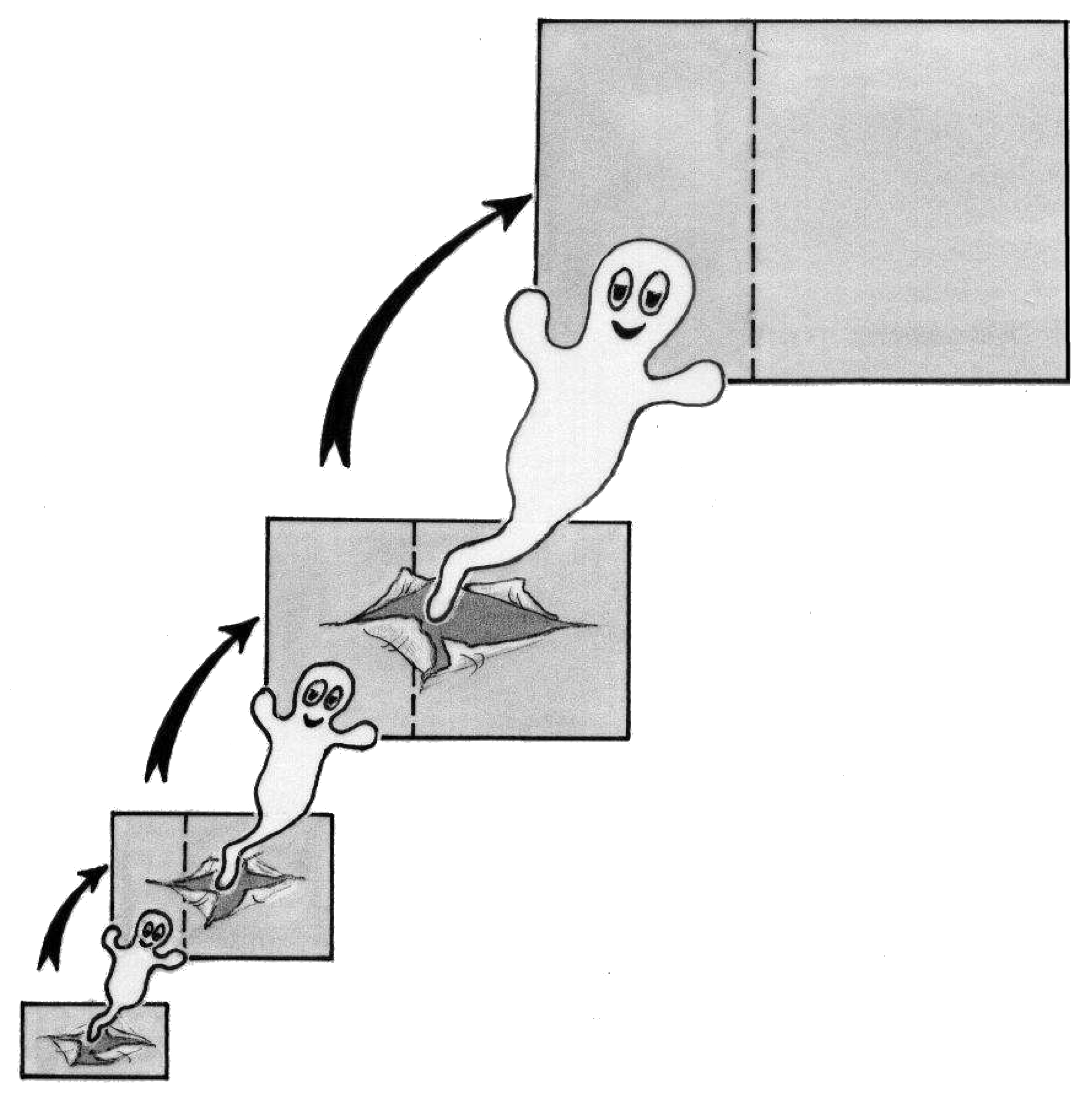
\includegraphics[width=15cm]{fantome}   
      \end{center}
      
      \bigskip

      Par groupes, vous effectuerez les recherches, puis rendrez une fiche récapitulative où figureront votre raisonnement, la modélisation et les calculs effectués.

   \vfill \hfill {\it\footnotesize D'après \og La résolution de problèmes mathématiques au collège \fg, MENJS, 2021.}

\end{Maquette}
    \pagebreak
    \graphicspath{{../../S16_Calculs_avec_des_nombres_relatifs/Images/}}

\themeN
\chapter{Calculs avec des nombres relatifs}
\label{S16}

\programme%
   {\item Somme et différence de nombres décimaux.}
   {\item Calculer avec des nombres décimaux relatifs.}

\vfill

\begin{debat}{Débat : Brahmagupta et l'invention du 0}
   {\bf Brahmagupta} est un mathématicien indien né en 598. Dans l'un de ses ouvrages, le {\it Brahma Sphuta Siddhanta}, il présente les règles d'arithmétique qui concernant les nombres positifs (qu'il appelle les biens) et les nombres négatifs (qu'il appelle les dettes) par des calculs de pertes et de profits. Il définit ainsi le zéro comme la différence d’un nombre par lui-même. Par exemple, voilà comment il exprime les opérations usuelles :
   \begin{itemize}
      \item zéro soustrait d’une dette est une dette ;
      \item zéro soustrait d’un bien est un bien ;
      \item zéro soustrait de zéro est zéro ;
      \item une dette soustraite de zéro est un bien ;
      \item un bien soustrait de zéro est une dette.
   \end{itemize}
   \tcblower
      {\psset{unit=0.9}
      \begin{pspicture}(0,0.5)(11,5.5)
         \psset{fillstyle=solid}
         \psellipse[fillcolor=Crimson!50](2,4.3)(1.3,0.8)
         \rput(2,4.6){\it indien}
         \rput(2,4){\bf sunya}
         \psline{->}(3.5,4.3)(4.5,4.3)
         \psellipse[fillcolor=Crimson!40](6,4.3)(1.3,0.8)
         \rput(6,4.6){\it arabe}
         \rput(6,4){\bf sifr}
         \psline{->}(7.5,4.3)(9,3.9) %
         \psellipse[fillcolor=Crimson!30](9.5,3)(1.3,0.8)
         \rput(9.5,3.3){\it latin}
         \rput(9.5,2.7){\bf zephirum}
         \psline{->}(9,2.1)(7.5,1.7)
         \psellipse[fillcolor=Crimson!20](6,1.7)(1.3,0.8)
         \rput(6,2){\it italien}
         \rput(6,1.4){\bf zephiro}
         \psellipse[fillcolor=Crimson!10](2,1.7)(1.3,0.8)
         \rput(2,2){\it français}
         \rput(2,1.4){\bf zéro}
         \psline{<-}(3.5,1.7)(4.5,1.7)    
      \end{pspicture}}
\end{debat}

\hfill {\gray Vidéo : \href{https://www.youtube.com/watch?v=KuJERDWGMw0}{\bf Addition et soustraction de nombres relatifs}, site Internet {\it Rapémathiques}, d'A'Rieka.}


%%% Approche %%%
\begin{Maquette}[Cours]{Theme={Activité d'approche},Couleur={SteelBlue}}

   \AAtitre{La pêche mystérieuse}

      {\it Objectifs : effectuer des additions et des soustractions avec des nombres entiers relatifs.}

      \begin{AActivite}

         Sept amis jouent à la fête foraine au jeu de la pêche mystérieuse, ils gagnent ou il perdent des points selon les objets qu'ils \og pêchent \fg. Voilà les points qu'ils peuvent gagner : \par
         \begin{pspicture}(0,1.5)(15,3.25)
            \rput(2,2.25){\psscalebox{0.4}{\psBill}}
            \rput(4,2.5){\it\textcolor{SteelBlue}{Billy}}
            \rput(4,2){\it\textcolor{SteelBlue}{+150 points}}
            \rput{-30}(6,2.4){\psscalebox{0.55}{\psBird}}
            \rput(9.5,2.5){\it\textcolor{SteelBlue}{Birdy}}
            \rput(9.5,2){\it\textcolor{SteelBlue}{+100 points}}
            \rput(12.5,1.5){\psKangaroo[fillcolor=brown]{1.7}}
            \rput(14.5,2.5){\it\textcolor{SteelBlue}{Skippy}}
            \rput(14.5,2){\it\textcolor{SteelBlue}{+50 points}}
         \end{pspicture}
         
         Cependant, certains objets font perdre des points : \par
         \begin{pspicture}(0,1.5)(15,3.25)
            \rput{-30}(2.2,2.25){\psscalebox{0.4}{\psAnt}}
            \rput(4,2.5){\it\textcolor{SteelBlue}{Antas}}
            \rput(4,2){\it\textcolor{SteelBlue}{-25 points}}
            \rput(6.7,1.7){\psscalebox{0.25}{\psFish[fillstyle=slope]}}         
            \rput(9.5,2.5){\it\textcolor{SteelBlue}{Fishas}}
            \rput(9.5,2){\it\textcolor{SteelBlue}{-75 points}}
            \rput(12.6,2.5){\psscalebox{0.45}{\psPig[fillcolor=pink](0,0)}}
            \rput(14.5,2.5){\it\textcolor{SteelBlue}{Pigas}}
            \rput(14.5,2){\it\textcolor{SteelBlue}{-125 points}}
         \end{pspicture}

         Compléter le tableau suivant des gains et des pertes. En déduire le total, puis le classement.
         \begin{center}
            {\hautab{0.9}
            \begin{tabular}{|C{9.5}|*3{C{1.7}|}}
               \hline
               \rowcolor{SteelBlue!50} Pêche & Gains & Pertes & Total \\
               \hline
               \begin{pspicture}(0,1.5)(9.5,3)
                  \rput[l](0,2.2){Lojain}
                  \rput(2,2.25){\psscalebox{0.3}{\psBill}}
                  \rput(3.5,2.25){\psscalebox{0.3}{\psBill}}
                  \rput(5,2.25){\psscalebox{0.3}{\psBill}}
                  \rput{-30}(5.8,2.3){\psscalebox{0.4}{\psBird}}
                  \rput(8.3,1.7){\psKangaroo[fillcolor=brown]{1.2}}
               \end{pspicture} & & & \\
               \hline
               \begin{pspicture}(0,1.5)(9.5,3)
                  \rput[l](0,2.2){Nihal}
                  \rput{-30}(2.2,2.25){\psscalebox{0.3}{\psAnt}}
                  \rput(3.7,2.3){\psscalebox{0.33}{\psPig[fillcolor=pink](0,0)}}
                  \rput(4.7,1.9){\psscalebox{0.2}{\psFish[fillstyle=slope]}} 
                  \rput(6.4,1.9){\psscalebox{0.2}{\psFish[fillstyle=slope]}} 
                  \rput{-30}(8.5,2.25){\psscalebox{0.3}{\psAnt}}
               \end{pspicture} & & & \\
               \hline
               \begin{pspicture}(0,1.5)(9.5,3)
                  \rput[l](0,2.2){Lorette}
                  \rput(2,2.25){\psscalebox{0.3}{\psBill}}
                  \rput(3.5,2.25){\psscalebox{0.3}{\psBill}}
                  \rput{-30}(4.2,2.3){\psscalebox{0.4}{\psBird}}
                  \rput(6.8,2.3){\psscalebox{0.33}{\psPig[fillcolor=pink](0,0)}}
                  \rput(7.8,1.9){\psscalebox{0.2}{\psFish[fillstyle=slope]}} 
               \end{pspicture} & & & \\
               \hline
               \begin{pspicture}(0,1.5)(9.5,3)
                  \rput[l](0,2.2){Lina}
                  \rput(2,2.3){\psscalebox{0.33}{\psPig[fillcolor=pink](0,0)}}
                  \rput(3.5,1.7){\psKangaroo[fillcolor=brown]{1.2}}
                  \rput(4.6,1.9){\psscalebox{0.2}{\psFish[fillstyle=slope]}} 
                  \rput(6.7,2.25){\psscalebox{0.3}{\psBill}}
                  \rput(8.4,1.7){\psKangaroo[fillcolor=brown]{1.2}}
               \end{pspicture} & & & \\
               \hline
               \begin{pspicture}(0,1.5)(9.5,3)
                  \rput[l](0,2.2){Milan}
                  \rput{-30}(2,2.25){\psscalebox{0.3}{\psAnt}}
                  \rput(3.5,1.7){\psKangaroo[fillcolor=brown]{1.2}}
                  \rput{-30}(5.2,2.25){\psscalebox{0.3}{\psAnt}}
                  \rput{-30}(6.8,2.25){\psscalebox{0.3}{\psAnt}}
                  \rput{-30}(8.5,2.25){\psscalebox{0.3}{\psAnt}}
               \end{pspicture} & & & \\
               \hline
               \begin{pspicture}(0,1.5)(9.5,3)
                  \rput[l](0,2.2){Marwa}
                  \rput{-30}(1.1,2.3){\psscalebox{0.4}{\psBird}}
                  \rput(3.5,1.7){\psKangaroo[fillcolor=brown]{1.2}}
                  \rput(4.6,1.9){\psscalebox{0.2}{\psFish[fillstyle=slope]}}
                  \rput(6.7,2.3){\psscalebox{0.35}{\psPig[fillcolor=pink](0,0)}}
                  \rput(8.2,1.7){\psKangaroo[fillcolor=brown]{1.2}}
               \end{pspicture} & & & \\
               \hline
               \begin{pspicture}(0,1.5)(9.5,3)
                  \rput[l](0,2.2){Roxane}
                  \rput(2.1,2.3){\psscalebox{0.35}{\psPig[fillcolor=pink](0,0)}}
                  \rput(3.6,2.3){\psscalebox{0.35}{\psPig[fillcolor=pink](0,0)}}
                  \rput(5.1,2.3){\psscalebox{0.35}{\psPig[fillcolor=pink](0,0)}}
                  \rput{-30}(5.8,2.3){\psscalebox{0.4}{\psBird}}
                  \rput{-30}(7.4,2.3){\psscalebox{0.4}{\psBird}}
               \end{pspicture} & & & \\
               \hline
            \end{tabular}}
         \end{center} \medskip
         Classement : \pointilles

   \end{AActivite}

\end{Maquette}


%%%Trace écrite %%%
\begin{Maquette}[Cours]{Theme={Trace écrite},Couleur={0.4[SteelBlue,Black]}}

   %%%1
   \section{Additionner deux nombres relatifs}

      \begin{methode*}{Somme de deux nombres relatifs}
         \begin{itemize}
            \item La somme de deux nombres relatifs ayant {\bf le même signe} s'obtient en ajoutant les distances à 0 et en mettant le même signe que les nombres. 
            \item La somme de deux nombres relatifs n'ayant {\bf pas le même signe} s'obtient en calculant la différence entre les distances à 0 et en mettant le signe du terme ayant la plus grande distance à 0.
         \end{itemize}
         \begin{exbmethode}
            \begin{multicols}{2}
               Nombres de même signe : \par
               $A =(+3)+(+7) = 3+7$ \par
               $B =(-12)+(-5)$ \par
               Nombres de signes différents : \par
               $C =(-7)+(+3) =(-7)+3$ \par
               $D =(+12)+(-5) =12+(-5)$
            \end{multicols}
            \tcblower
               \begin{multicols}{2}
                  $\bullet$ Le signe devant 3 et 7 est $+$ \par
                  on additionne 3 et 7 et on met le signe $+$ : $A =+10$. \par
                  On peut écrire $A =+(3+7) =+10 =10$. \par
                  $\bullet$ Le signe devant 12 et 5 est $-$ \par
                  on additionne 12 et 5 et on met le signe $-$ : $B =-17$. \par
                  On peut écrire $B =-(12+5) =-17$. \par
                  $\bullet$ Le signe devant 7 est $-$ et celui devant 3 est $+$ \par
                  on effectue la différence entre 3 et 7 et \par
                  on met le signe $-$ : $C =-(7-3) =-4$. \par
                  $\bullet$ Le signe devant 12 est $+$ et celui devant 5 est $-$ \par
                  on effectue la différence entre 5 et 12 et \par
                  on met le signe $+$ : $D =+(12-5) =+7 =7$. 
               \end{multicols}
         \end{exbmethode}
      \end{methode*}

      \begin{propriete*}{}
         La somme de deux nombres opposés vaut 0.
      \end{propriete*}

      \begin{exemple*}{}
         $E =(+2\,022)+(-2\,022) =(-2\,022)+(+2\,022) =2\,022-2\,022 =0$.
      \end{exemple*}

   %%%2
   \section{Soustraire deux nombres relatifs}

      \begin{propriete*}{}
         Soustraire un nombre revient à ajouter son opposé : $a-b=a+(-b)$.
      \end{propriete*}

      \begin{exemple*}{}
         $F =(+15,3)-(-5,1) =(+15,3)+(+5,1) =+(15,3+5,1) =+20,4 =20,4$ \par
         $G =(+2,4)-(+1,3)=(+2,4)+(-1,3) =+(2,4-1,3) =+1,1 =1,1$
      \end{exemple*}


      \begin{methode*}{Simplification d'expressions}
         Pour {\bf simplifier} les écritures dans les opérations :
         \begin{enumerate}
            \item on transforme chaque soustraction en addition de l'opposé ;
            \item on écrit l'expression en enlevant les parenthèses et les signes $+$ devant les nombres ;
            \item on peut éventuellement regrouper les termes de même signe afin de les calculer ensemble.
         \end{enumerate}
         \begin{exbmethode}
            On souhaite simplifier l'expression $H =(+1,2)+(+3,4)+(-1,5)-(+2,7)-(-5,7)$.
            \tcblower
               \begin{enumerate}
                  \item $H =(+1,2)+(+3,4)+(-1,5)+(-2,7)+(+5,7)$ \par
                  \item $H =1,2+3,4-1,5-2,7+5,7$ \par
                  \item $H =(1,2+3,4+5,7)-(1,5+2,7) =10,3-4,2 =6,1$.
               \end{enumerate}
         \end{exbmethode}
      \end{methode*}

\end{Maquette}


%%% Exercices %%%
\begin{Maquette}[Fiche,CorrigeFin,Colonnes=2]{}
   
   \begin{multicols}{2}

      \begin{exercice}[SLF] %1
         Effectuer les calculs suivants :
         \begin{enumerate}[label=\Alph*]
            \item $=(-12)+(-15) =\pointilles$
            \item $=(-20)+(+18) =\pointilles$
            \item $=(+21,5)+(-21,5) =\pointilles$
            \item $=(+10)+(-13) =\pointilles$
            \item $=(-3,5)+(+16) =\pointilles$
            \item $=(+13)+(+7) =\pointilles$
         \end{enumerate}
      \end{exercice}
      
      \begin{Solution}
         \begin{enumerate}[label=\Alph*]
            \item $=(-12)+(-15) =-(12+15) =\cor{-27}$
            \item $=(-20)+(+18) =-(20-18) =\cor{-2}$
            \item $=(+21,5)+(-21,5) =21,5-21,5 =\cor{0}$
            \item $=(+10)+(-13) =-(13-10) =\cor{-3}$
            \item $=(-3,5)+(+16) =+(16-3,5) =\cor{12,5}$
            \item $=(+13)+(+7) =+(13+7) =\cor{20}$
         \end{enumerate}
      \end{Solution}
      
      
      \begin{exercice}[SLF] %2
         Pour chaque cas, transformer la soustraction en addition puis effectuer le calcul.
         \begin{enumerate}[label=\Alph*]
            \item $=(-12)-(+15) =\pointilles$
            \item $=(-45)-(-41) =\pointilles$
            \item $=(+32)-(+27) =\pointilles$
            \item $=(-2)-(+2,7) =\pointilles$
            \item $=(-1,4)-(-2,3) =\pointilles$
         \end{enumerate}
      \end{exercice}
      
      \begin{Solution}
         \begin{enumerate}[label=\Alph*]
            \item $=(-12)-(+15)=(-12)+(-15) =-(12+15) =\cor{-27}$
            \item $=(-45)-(-41) =(-45)+(+41) =-(45-41) =\cor{-4}$
            \item $=(+32)-(+27) =(+32)+(-27) =+(32-27) =\cor{5}$
            \item $=(-2)-(+2,7) =(-2)+(-2,7) =-(2+2,7) =\cor{-4,7}$
            \item {\small$=(-1,1)-(-3,7) =(-1,1)+(+3,7) =+(3,7-1,1) =\cor{2,6}$}
         \end{enumerate}
      \end{Solution}
      
      
      \begin{exercice}[Dur] %3
         Effectuer les calculs suivants en simplifiant.
         \begin{enumerate}[label=\Alph*]
            \item $=(+12)+(-11)+(+25)+(-17)$
            \item $=(-2,1)+(-9)+(+6,4)+(-8,3)$
            \item $=(+14)+(-7)+(+2)+(-3,75)+(-5,25)$
            \item $=(+13,5)+(-8,1)+(-6,9)+(-5,5)$
         \end{enumerate}
      \end{exercice}
      
      \begin{Solution}
         \begin{enumerate}[label=\Alph*]
            \item $=(+12)+(-11)+(+25)+(-17)$ \par
               $=+(12+25)-(11+17) =+37-28 =\cor{9}$
            \item $=(-2,1)+(-9)+(+6,4)+(-8,3)$ \par
               $=+(6,4)-(2,1+9+8,3) =+6,4-19,4 =\cor{-13}$
            \item $=(+14)+(-7)+(+2)+(-3,75)+(-5,25)$ \par
               $=+(14+2)-(7+3,75+5,25) =+16-16 =\cor{0}$
            \item $=(+13,5)+(-8,1)+(-6,9)+(-5,5)$ \par
               $=+(13,5)-(8,1+6,9+5,5) =+13,5-20,5 =\cor{-7}$
         \end{enumerate}
      \end{Solution}
      
      
      \begin{exercice}[Dur] %4
         Pour chaque expression, regrouper astucieusement puis calculer.
         \begin{enumerate}[label=\Alph*]
            \item $=-14+5-2$
            \item $=-2-23+33$
            \item $=18-7+9-18-9+7$
            \item $=6,4+11,5-3,4+0,5$
            \item $=13,36+4+6-3,36$
         \end{enumerate}
      \end{exercice}
      
      \begin{Solution}
         \begin{enumerate}[label=\Alph*]
            \item $=-14+5-2 =5-(14+2) =5-16 =\cor{-11}$
            \item $=-2-23+33 =33-(2+23) =33-25 =\cor{8}$
            \item $=18-7+9-18-9+7$ \par
               $=(18-18)+(9-9)+(7-7) =0+0+0 =\cor{0}$
            \item $=6,4+11,5-3,4+0,5$ \par
               $=(6,4-3,4)+(11,5+0,5) =3+12 =\cor{15}$
            \item $=13,36+4+6-3,36$ \par
               $=(13,36-3,36)+(4+6) =10+10 =\cor{20}$
         \end{enumerate}
      \end{Solution}
      
      
      \begin{exercice} %5
         Dans le monde entier, les heures locales sont fixées par rapport à l'heure universelle (UT). Paris est à UT, New York est à UT $-\Temps{;;;6}$ et New Delhi est à UT $+\Temps{;;;4;30}$.
         \begin{enumerate}
            \item Cyrine, qui est à Montpellier, appelle à New York à \Temps{;;;20} et téléphone pendant trois quarts d'heure. Quelle heure est-il à New York à la fin de l'appel ?
            \item Après ce coup de téléphone, Cyrine peut-elle raisonnablement appeler à New Delhi ?
         \end{enumerate}
      \end{exercice}
      
      \begin{Solution}
         Montpellier est à la même UT que Paris. \par
         \begin{enumerate}
            \item \Temps{;;;20;0} \quad $\xrightarrow{+\Temps{;;;;45}}$ \quad \Temps{;;;20;45}. \par
               Donc, Cyrine termine son appel à \Temps{;;;20;45}. \par \smallskip
               \Temps{;;;20;45} \quad $\xrightarrow{-\Temps{;;;6}}$ \quad \Temps{;;;14;45}. \par
               À cette heure, il est \cor{\Temps{;;;14;45}} à New-York.
            \item Pour New Delhi, il faut ajouter \Temps{;;;4;30} à l'heure de Paris, on peut décomposer ainsi : \par \smallskip
               \Temps{;;;20;45} \quad $\xrightarrow{+\Temps{;;;4}}$ \quad \Temps{;;;24;45} = \Temps{;;;0;45} \par \smallskip
               \Temps{;;;0;45} \quad $\xrightarrow{+\Temps{;;;;30}}$ \quad \Temps{;;;1;15} \par \smallskip
               Il est \Temps{;;;1;15} du matin donc, \cor{il n'est pas raisonnable d'appeler en Inde !}
         \end{enumerate}
      \end{Solution}
      
      
      \begin{exercice} %6
         Dans un QCM de dix questions, une réponse juste rapporte 4 points, une absence de réponse 0 point et une mauvaise réponse enlève 3 points.
         \begin{enumerate}
            \item Bilel a 2 bonnes réponses et 8 mauvaises. Quelle est sa note ?
            \item Quelle est la plus mauvaise note qu'il est possible d'obtenir à ce QCM ? La meilleure note ?
            \item Jasmine a obtenu 14 points. Donner une combinaison possible pour obtenir ce résultat.
         \end{enumerate}
      \end{exercice}
      
      \begin{Solution}
         \begin{enumerate}
            \item 2 bonnes réponses donnent  $2\times4\text{ points} =8\text{ points}$ ; \par
               8 mauvaises réponses enlèvent $8\times3\text{ points} =24\text{ points}$. \par
               Or, $+8-24 =-(24-8) =-16$ donc, \par
               la note de Bilel est de \cor{$-16$ points}.
            \item La plus mauvaise note est obtenue lorsque l'on donne 10 mauvaises réponses, soit $-(10\times3\text{ points}) =\cor{-30\text{ points}}$ ; \par
               La meilleure note est obtenue lorsque l'on donne 10 bonnes réponses, soit  $+(10\times4\text{ points}) =\cor{+40\text{ points}}$. \par
            \item Jasmine peut, par exemple, avoir donné :
               \begin{itemize}
                  \item \cor{5 bonnes réponses}, soit +20 points ;
                  \item \cor{2 mauvaises réponses}, soit $-6$ points ; 
                  \item \cor{3 questions sans réponse}, soit 0 point.
               \end{itemize}
            Cela donne bien : $+20-6+0 =14$.
         \end{enumerate}
      \end{Solution}
      
      
      \begin{exercice} %7
         Voici un programme de calcul :
         \begin{center}
            \ProgCalcul[Enonce,Largeur=5cm]{Choisir un nombre,Ajouter \num{-3},Retirer \num{-1.5},Donner l'opposé du résultat}
         \end{center}
         \begin{enumerate}
            \item Appliquer ce programme au nombre $-2,5$ puis 0.
            \item Quel nombre faut-il choisir pour obtenir 6 ?
            \item Soit $x$ le nombre de départ, donner l'expression finale en fonction de $x$.
         \end{enumerate}
      \end{exercice}
      
      \begin{Solution}
         \begin{enumerate}
            \item $-2,5 \xrightarrow[-3]{+(-3)} -5,5 \xrightarrow[+1,5]{-(-1,5)} -4 \xrightarrow{\text{opposé}} \cor{4}$ \par \smallskip
               \quad\, $0 \xrightarrow[-3]{+(-3)} -3 \xrightarrow[+1,5]{-(-1,5)} -1,5 \xrightarrow{\text{opposé}} \cor{1,5}$ \par \smallskip
            \item On effectue les opérations \og à l'envers \fg. \par \smallskip
               \quad\, $6 \xrightarrow{\text{opposé}} -6 \xrightarrow[-1,5]{+(-1,5)} -7,5  \xrightarrow[+3]{-(-3)}\cor{-4,5}$ \par \smallskip
            \item $x \xrightarrow[-3]{+(-3)} x-3 \xrightarrow[+1,5]{-(-1,5)} x-3+1,5$ \par
               \quad\; $=x-1,5 \xrightarrow{\text{opposé}}\cor{-x+1,5}$. \par \smallskip
         \end{enumerate}
      \end{Solution}
      
      
      \begin{exercice}[SLF] %8
         Compléter les pyramides suivantes sachant que chaque nombre est la somme des nombres se trouvant dans les deux cases juste en dessous.  \par \medskip
         \PyramideNombre[Etages=4,Largeur=9mm]{\num{-1},~,~,~,8,~,~,\num{-4},~,\num{-7}}
         \quad
         \PyramideNombre[Etages=4,Largeur=9mm]{6,~,~,~,\num{-7},~,~,\num{-5},~,\num{-3}}
         \vskip5mm
         \PyramideNombre[Etages=4,Largeur=9mm]{\num{-1.5},~,~,~,3,~,~,\num{-5},~,\num{-5}}
         \quad
         \PyramideNombre[Etages=4,Largeur=9mm]{\num{6.3},~,~,~,\num{7.2},~,~,~,\num{-3.1},\num{-5.2}}
      \end{exercice}
      
      \begin{Solution}
         \medskip
         \PyramideNombre[Etages=4,Largeur=9mm,Hauteur=8mm,Couleur=1.5RoyalBlue]{\num{-1},*9,*\num{-21},*30,8,*\num{-12},*9,\num{-4},*\num{-3},\num{-7}}   
         \quad
         \PyramideNombre[Etages=4,Largeur=9mm,Hauteur=8mm,Couleur=1.5RoyalBlue]{6,*\num{-13},*15,*\num{-15},\num{-7},*2,*0,\num{-5},*2,\num{-3}}
         \vskip3mm
         \PyramideNombre[Etages=4,Largeur=9mm,Hauteur=8mm,Couleur=1.5RoyalBlue]{\num{-1.5},*\num{4,5},*\num{-12,5},*\num{20,5},3,*\num{-8},*8,\num{-5},*0,\num{-5}}
         \quad
         \PyramideNombre[Etages=4,Largeur=9mm,Hauteur=8mm,Couleur=1.5RoyalBlue]{\num{6.3},*\num{0,9},*\num{-12,2},*\num{16,4},\num{7.2},*\num{-9,3},*\num{6,2},*\num{-2,1},\num{-3.1},\num{-5.2}}
      \end{Solution}

   \end{multicols}

\end{Maquette}


%%% Récré %%%
\begin{Maquette}[Cours]{Theme={Activité récréative},Couleur={IndianRed}}
    
   \ARtitre{Décryptage}

      Décrypter les codes suivants utilisé par l'agent Zérozérossette sachant que chaque symbole correspond à un nombre entier relatif et que la somme de chaque ligne et de chaque colonne est indiquée en bout de celle-ci. \par \bigskip

      \begin{center}
         {\hautab{1.8}
         \begin{tabular}{*{7}{C{0.5}}}
            \Large\ding{101} & $+$ & \Large\ding{101} & $+$ & \Large\ding{40} & $=$ & \large 16 \\
            $+$ & & $+$ & & $+$ & & \\
            \Large\ding{168} & + & \Large\ding{168} & + & \Large\ding{168} & $=$ & \large 9 \\
            $+$ & & $+$ & & $+$ & & \\
            \Large\ding{40} & + & \Large\ding{52} & + & \Large\ding{168} & $=$ & \large 18 \\
            $=$ & & $=$ & & $=$ & & \\
            \large 14 & & \large 17 & & \large 12 & & \\
         \end{tabular}
         \hskip3cm
         \begin{tabular}{*{7}{C{0.5}}}
            \Large\ding{101} & $+$ & \Large\ding{101} & $+$ & \Large\ding{101} & $=$ & \large $-3$ \\
            $+$ & & $+$ & & $+$ & & \\
            \Large\ding{40} & + & \Large\ding{168} & + & \Large\ding{101} & $=$ & \large $-3$ \\
            $+$ & & $+$ & & $+$ & & \\
            \Large\ding{52} & + & \Large\ding{52} & + & \Large\ding{168} & $=$ & \large 6 \\
            $=$ & & $=$ & & $=$ & & \\
            \large 6 & & \large 0 & & \large $-6$ & & \\
         \end{tabular}

         \vskip8mm
         
         \begin{tabular}{|p{2cm}|p{2cm}|}
            \hline
            \Large\ding{101} = & \Large\ding{40} = \\
            \hline
            \Large\ding{168} = & \Large\ding{52} = \\
            \hline
         \end{tabular}
         \hskip4.5cm
         \begin{tabular}{|p{2cm}|p{2cm}|}
            \hline
            \Large\ding{101} = & \Large\ding{40} = \\
            \hline
            \Large\ding{168} = & \Large\ding{52} = \\
            \hline
         \end{tabular}

         \vskip18mm
         
         {\setlength{\tabcolsep}{0mm}
         \begin{tabular}{*{9}{C{0.8}}}
            \Large\ding{101} & $+$ & \Large\ding{40} & $+$ & \Large\ding{40} & $+$ & \Large\ding{101} & $=$ & \large 2 \\
            $+$ & & $+$ & & $+$ & & $+$ & \\
            \Large\ding{40} & $+$ & \Large\ding{40} & $+$ & \Large\ding{40} & $+$ & \Large\ding{168} & $=$ & \large 9 \\
            $+$ & & $+$ & & $+$ & & $+$ & \\
            \Large\ding{40} & + & \Large\ding{168} & + & \Large\ding{52} & $+$ & \Large\ding{36} & $=$ & \large $-7$ \\
            $=$ & & $=$ & & $=$ & & $=$ & \\
            \large 3 & & \large 7 & & \large $-1$ & & \large $-5$ & & \\ 
         \end{tabular}
         \hskip2cm
         \begin{tabular}{*{9}{C{0.8}}}
            \Large\ding{52} & $+$ & \Large\ding{52} & $+$ & \Large\ding{168} & $+$ & \Large\ding{168} & $=$ & \large \!\!$-158$ \\
            $+$ & & $+$ & & $+$ & & $+$ & \\
            \Large\ding{40} & $+$ & \Large\ding{52} & $+$ & \Large\ding{36} & $+$ & \Large\ding{36} & $=$ & \large \!$-19$ \\
            $+$ & & $+$ & & $+$ & & $+$ & \\
            \Large\ding{101} & + & \Large\ding{52} & + & \Large\ding{40} & $+$ & \Large\ding{52} & $=$ & \large \!$-86$ \\
            $=$ & & $=$ & & $=$ & & $=$ & \\
            \large \!$-32$ & & \large \!\!$-162$ & & \large \!$-37$ & & \large \!$-32$ & & \\ 
         \end{tabular}}

         \vskip8mm
      
         \begin{tabular}{|p{2cm}|p{2cm}|p{2cm}|}
            \hline
            \Large\ding{101} = & \Large\ding{40} = & \Large\ding{168} = \\
            \hline
            \Large\ding{36} = & \Large\ding{52} = \\
            \cline{1-2}
         \end{tabular}
         \hskip2cm
         \begin{tabular}{|p{2cm}|p{2cm}|p{2cm}|}
            \hline
            \Large\ding{101} = & \Large\ding{40} = & \Large\ding{168} = \\
            \hline
            \Large\ding{36} = & \Large\ding{52} = \\
            \cline{1-2}
         \end{tabular}}
      \end{center}

\end{Maquette}
    \pagebreak
    \graphicspath{{../../S17_Inegalite_triangulaire/Images/}}

\themeG
\chapter{L'inégalité triangulaire}
\label{S17}

\programme%
   {\item Triangle : inégalité triangulaire.}
   {\item Mettre en \oe uvre ou écrire un protocole de construction d’une figure géométrique.}

\vfill

\begin{debat}{Débat :  des instruments de navigation astronomique anciens}
   De tous temps, les hommes ont cherché à se repérer. Avant l’avènement de l'électronique et des GPS, de multiples instruments ont pu exister, par exemple : 
   \tcblower
      \begin{tabular}{*{4}{C{3.6}}}
         
\includegraphics[height=3cm]{astrolabe} & 
\includegraphics[height=3cm]{boussole}  & 
\includegraphics[height=3cm]{octant} & 
\includegraphics[height=3cm]{sextant} \\
         Astrolabe : & Boussole : & Octant : & Sextant : \\
         représentation plane de la sphère céleste & indique le nord magnétique & mesure la hauteur des corps célestes (45°) & mesure la hauteur des corps célestes (60°) \\
         Antiquité & {\small XIII}\up{e} & {\small XVIII}\up{e} & {\small XVIII}\up{e} \\
   \end{tabular}
\end{debat}

\hfill {\gray Vidéo : \href{https://www.youtube.com/watch?v=E0KvuFx0Mr8}{\bf Du kamal au GPS 1} et \href{https://www.youtube.com/watch?v=Jv21tvyZokk}{\bf Du kamal au GPS 2}, chaîne Youtube du {\it Musée national de la marine}.}


%%% Approche %%%
\begin{Maquette}[Cours]{Theme={Activité d'approche},Couleur={SteelBlue}}

   \AAtitre{Avec des allumettes}

      {\it Objectifs : construire des triangles sous contraintes.}

      \begin{AActivite}

         Devant vous, vous avez dix allumettes. Pour chacune des questions suivantes, faire la construction si elle est possible avec des allumettes puis faire un dessin pour schématiser la situation.
         \begin{enumerate}
            \item
            \begin{enumerate}
               \item Aligner quatre allumettes en les plaçant les unes à côté des autres.
               \medskip
               \begin{center}
                  \includegraphics[width=3cm]{allumette}\includegraphics[width=3cm]{allumette}\includegraphics[width=3cm]{allumette}\includegraphics[width=3cm]{allumette}
               \end{center}
               \medskip
               \item À partir de ce segment de longueur 4 allumettes, construire un triangle dont les deux autres côtés ont pour longueur trois allumettes. \par \vskip2.5cm
               \item En utilisant les dix allumettes, construire un triangle différent du précédent dont un des côtés a pour longueur quatre allumettes. Quelles sont les longueurs de ses côtés ? \par \vskip2.5cm
            \end{enumerate}
            \item En utilisant les dix allumettes, est-il possible de construire un triangle dont un des côtés a pour longueur six allumettes ? sept allumettes ? Expliquer. \par \vskip2.5cm
            \item En utilisant les dix allumettes, peut-on construire un triangle dont un côté a pour longueur cinq allumettes ? Que constate-t-on dans ce cas ? \par \vskip2.5cm
            \item On veut maintenant construire un triangle de périmètre 12 allumettes dont les côtés ont pour longueur un nombre entier d'allumettes. Donner toutes les solutions possibles ainsi que la nature des triangles. \vspace*{2.5cm} 
         \end{enumerate}

   \end{AActivite}

\end{Maquette}


%%% cours %%%
\begin{Maquette}[Cours]{Theme={Trace écrite},Couleur={0.4[SteelBlue,Black]}}

   %%%1
   \section{L'inégalité triangulaire}

      \begin{propriete*}{}
         Dans un triangle, la longueur d'un côté est toujours inférieure à la somme des longueurs des deux autres côtés. S'il y a égalité, alors les trois points sont alignés et le triangle est \og plat \fg.
      \end{propriete*}

      \begin{exemple*}{}
         \begin{minipage}{6cm}
            {\small
            \begin{pspicture}(-0.75,-0.3)(3.5,2.5)
               \pstGeonode[CurveType=polygon,PointSymbol=none,PosAngle={180,90,0}](0,0){A}(2.5,2){C}(3.5,0){B}
               \pstLabelAB[offset=-3mm]{A}{B}{\Lg{3,5}}
               \pstLabelAB{A}{C}{\Lg{3,2}}
               \pstLabelAB{C}{B}{\Lg{2,2}}
            \end{pspicture}}
         \end{minipage}
         \begin{minipage}{10cm}
            Dans le triangle $ABC$, on a :
            \begin{itemize}
               \item $AC =\Lg{3,2}$ et $AB+BC =\Lg{5,7}$ donc $AC\leq AB+BC$ ;
               \item $CB =\Lg{2,2}$ et $CA+AB =\Lg{6,7}$ donc $CB\leq CA+AB$ ;
               \item $BA =\Lg{3,5}$ et $BC+CA =\Lg{5,4}$ donc $BA\leq BC+CA$.
            \end{itemize}
         \end{minipage}
      \end{exemple*}
   
      Remarque : dans la pratique, on vérifie seulement que la longueur du plus grand côté est plus grande que la somme des longueurs des deux autres côtés.
   
   
   %%%2
   \section{Construction de triangles}
   
      Pour construire un triangle, il faut au minimum trois données :
      \begin{itemize}
         \item soit trois longueurs ;
         \item soit deux longueurs et l'angle compris entre les segments correspondants aux longueurs données ;
         \item soit une longueur et les deux angles adjacents au segment correspondant à la longueur donnée ;
         \item si on a trois angles, on pourra construire un triangle mais il ne sera pas unique : tous les triangles seront semblables (des agrandissements ou des réductions du même triangle).
      \end{itemize}
   
   \begin{methode*}{Construire un triangle connaissant trois longueurs}
      Pour construire un triangle $ABC$ dont on connaît les longueurs des trois côtés :
      \begin{itemize}
         \item on trace à la règle graduée l'un des côtés (en général le plus grand), par exemple $[AB]$ ;
         \item on trace un arc de cercle de centre $A$ et de rayon $AC$ ;
         \item on trace un arc de cercle de centre $B$ et de rayon $BC$ ;
         \item le point $C$ se situe à l'intersection des deux arcs de cercle.
      \end{itemize}
      \begin{exbmethode}
         Tracer le triangle $ABC$ tel que : $AB =\Lg{3,5}$ ; $BC =\Lg{2,2}$ ; $CA =\Lg{3,2}$.
         \tcblower
            {\small
            \psset{unit=0.8}
            \begin{pspicture}(0,-3)(4.5,3.3)
               \pstGeonode[PosAngle={225,-45}](0,0){A}(3.5,0){B}
               \pstLineAB{A}{B}
               \pstLabelAB[offset=-3mm]{A}{B}{\Lg{3,5}}
               \rput(1.7,-2.5){\parbox{3cm}{\it tracer le segment $[AB]$ de longueur \Lg{3,5}}}
            \end{pspicture}
            \begin{pspicture}(-0.5,-3)(5,3.3)
               \pstGeonode[PosAngle={225,-45}](0,0){A}(3.5,0){B}
               \pstLineAB{A}{B}
               \psset{linecolor=DodgerBlue}
               \psarc(0,0){3.2}{30}{60}
               \rput{55}(0.8,1.3){\textcolor{DodgerBlue}{\Lg{3,2}}}
               \compas{1.5}{1.2}{55}{0.9}{34.5}
               \rput(1.7,-2.5){\parbox{3.5cm}{\it tracer un arc de cercle de centre $A$ et de rayon $\Lg{3,2}$}}
            \end{pspicture}
            \begin{pspicture}(0,-3)(5,3.3)
               \pstGeonode[PosAngle={225,-45}](0,0){A}(3.5,0){B}
               \pstLineAB{A}{B}
               \psset{linecolor=DodgerBlue}
               \psarc(0,0){3.2}{30}{60}
               \psset{linecolor=Crimson}
               \psarc[fillstyle=none](3.5,0){2.2}{90}{130}
               \rput{-45}(2.8,0.8){\textcolor{Crimson}{\Lg{2,2}}}
               \compas{3.3}{1.1}{130}{0.9}{23}
               \rput(1.7,-2.5){\parbox{3.5cm}{\it tracer un arc de cercle de centre $A$ et de rayon $\Lg{2,2}$}}
            \end{pspicture}
            \begin{pspicture}(0,-3)(4,3.3)
               \pstGeonode[CurveType=polygon,PointSymbol=none,PosAngle={225,90,-45}](0,0){A}(2.5,2){C}(3.5,0){B}
               \rput(1.8,-2.5){\parbox{3.5cm}{\it Placer le point $C$, intersection des deux arcs de cercle}}
            \end{pspicture}}
         \end{exbmethode}
   \end{methode*}
   

   \begin{methode*}{Construire un triangle connaissant deux longueurs et un angle}
      Pour construire un triangle $ABC$ dont on connaît la longueur de deux côtés ainsi que l'angle entre ces cotés :
      \begin{itemize}
         \item on trace à la règle graduée l'un des côtés donnés, par exemple $[AB]$ ;
         \item on trace au rapporteur l'angle donné à partir du segment tracé ;
         \item on trace à la règle graduée le deuxième segment de longueur donnée le long du support de l'angle tracé juste avant ;
         \item le point $C$ se trouve à l'extrémité de ce segment.
      \end{itemize}
      \begin{exbmethode}
         Tracer le triangle $ABC$ tel que : $AB =\Lg{3,5}$ ; $\widehat{BAC} =39°$ et $CA =\Lg{3,2}$.
         \tcblower
            {\small
            \psset{unit=0.8}
            \begin{pspicture}(-0.5,-2.5)(4,3)
               \pstGeonode[PosAngle={225,-45}](0,0){A}(3.5,0){B}
               \pstLineAB{A}{B}
               \pstLabelAB[offset=-3mm]{A}{B}{\Lg{3,5}}
               \rput(1.75,-2){\parbox{3cm}{\it tracer le segment $[AB]$ de longueur \Lg{3,5}}}
            \end{pspicture}
            \hskip1cm
            \begin{pspicture}(-3,-2.5)(4,3)
               \pstGeonode[PosAngle={225,-45}](0,0){A}(3.5,0){B}
               \pstLineAB{A}{B}  
               \psset{linecolor=DodgerBlue}
               \rapporteur{0}{0}{0}{0.75}
               \psline(0,0)(4;38.66)
               \psarc(0,0){1}{0}{39}
               \rput(1.4,0.4){\textcolor{DodgerBlue}{39°}}
               \rput(0.4,-2){\parbox{5.2cm}{\it tracer la demi-droite d'origine $A$ faisant un angle de 39° avec le segment $[AB]$}}
            \end{pspicture}
            \hskip1cm
            \begin{pspicture}(-0.5,-2.5)(4,3)
               \pstGeonode[CurveType=polygon,PointSymbol=none,PosAngle={225,90,-45}](0,0){A}(2.5,2){C}(3.5,0){B}
               \psline(0,0)(4;38.66) 
               \psline[linecolor=Crimson,linewidth=0.8mm](0,0)(2.5,2)
               \rput{40}(1.1,1.4){\textcolor{Crimson}{3,2 cm}}
               \rput(1.75,-2){\parbox{4cm}{\it placer le point $C$ sur cette demi-droite tel que $AC =\Lg{3,5}$}}
            \end{pspicture}}
      \end{exbmethode}
   \end{methode*}
   
   Remarque : dans toute construction d'un triangle $ABC$, on a deux choix de construction pour $C$, d'un côté ou de l'autre du segment $[AB]$. \medskip

   \begin{methode*}{Construire un triangle connaissant une longueur et deux angles}
      Pour construire un triangle $ABC$ dont on connaît la longueur d'un côté ainsi que ses deux angles adjacents :
      \begin{itemize}
         \item on trace à la règle graduée le côté donné, par exemple $[AB]$ ;
         \item on trace au rapporteur les deux angles donnés à partir du segment tracé ;
         \item les deux demi-droites tracées grâce au rapporteur se coupent au point $C$.
      \end{itemize}
      \begin{exbmethode}
         Tracer le triangle $ABC$ tel que : $AB =\Lg{3,5}, \widehat{BAC} =39°$ et $\widehat{ABC} =63°$
         \tcblower
            {\small
            \psset{unit=0.8}
            \begin{pspicture}(0,-3)(4,3.5)
               \pstGeonode[PosAngle={225,-45}](0,0){A}(3.5,0){B}
               \pstLineAB{A}{B}
               \rput(1.75,-0.25){\Lg{3,5}}
               \rput(1.75,-2){\parbox{3cm}{\it tracer le segment $[AB]$ de longueur \Lg{3,5}}}
            \end{pspicture}
            \hskip6mm
            \begin{pspicture}(-3,-3)(4,3.5)
               \pstGeonode[PosAngle={225,-45}](0,0){A}(3.5,0){B}
               \pstLineAB{A}{B}  
               \psset{linecolor=DodgerBlue}
               \rapporteur{0}{0}{0}{0.75}
               \psline(0,0)(4;38.66)
               \psarc(0,0){1}{0}{39}
               \rput(1.4,0.4){\textcolor{DodgerBlue}{39°}}
               \rput(0.4,-2){\parbox{5.2cm}{\it tracer la demi-droite d'origine $A$ faisant un angle de 39° avec le segment $[AB]$}}
            \end{pspicture}
            \hskip6mm
            \begin{pspicture}(-0.5,-3)(6.5,3.5)
               \pstGeonode[PointSymbol=none,PosAngle={225,-45}](0,0){A}(3.5,0){B}
               \pstLineAB{A}{B}
               \psline{->}(2.5,3.2)(2.5,2)
               \psset{linecolor=DodgerBlue}
               \psline(0,0)(4;38.66)
               \psset{linecolor=Crimson}
               \rapporteur{4.65}{0}{0}{0.75}
               \psline(3.5,0)(2.05,2.8)
               \psarc(3.5,0){0.8}{117}{180}
               \rput(2.5,0.6){\textcolor{Crimson}{63°}}
               \rput(2.5,3.5){C}
               \rput(3,-2.25){\parbox{5.6cm}{\it tracer la demi-droite d'origine $B$ faisant un angle de 63° avec le segment $[BA]$. Placer le point $C$ à l'intersection des deux demi-droites}}
            \end{pspicture}}
         \end{exbmethode}
   \end{methode*}

\end{Maquette}


%%% Exercices %%%
\begin{Maquette}[Fiche,CorrigeFin,Colonnes=2]{}

   \begin{multicols}{2}

      \begin{exercice} %1
         Ces triangles sont-ils constructibles (ils ne sont pas tracés en vraie grandeur) ?
         \begin{center}
            {\small
            \begin{pspicture}(-0.5,-0.5)(3,2.5)
               \pstTriangle[PointSymbol=none](0,0){G}(3,0){L}(1,2){E}
               \pstLabelAB[offset=-3mm]{G}{L}{\Lg{8}}
               \pstLabelAB{G}{E}{\Lg{3}}
               \pstLabelAB{E}{L}{\Lg{3,5}}
            \end{pspicture}
            \begin{pspicture}(-0.5,-1.5)(3.5,1)
               \pstTriangle[PointSymbol=none](0,0){E}(3,0){U}(1.5,1){A}
               \pstLabelAB[offset=-3mm]{E}{U}{\Lg{6,2}}
               \pstLabelAB{E}{A}{\Lg{3,1}}
                  \pstSegmentMark[MarkAngle=90]{E}{A}
                  \pstSegmentMark[MarkAngle=90]{A}{U}
            \end{pspicture} 
         
            \psset{unit=1.5}
            \begin{pspicture}(0,-1)(3,1.5)
               \pstTriangle[PointSymbol=none](0,0){G}(3,0){Z}(2.7,1){A}
               \pstLabelAB[offset=-3mm]{G}{Z}{\Lg{6,3}}
               \pstLabelAB{A}{Z}{\Lg{2}}
               \pstSegmentMark[MarkAngle=90]{Z}{G}
               \pstSegmentMark[MarkAngle=90]{A}{G}
            \end{pspicture} 
            \begin{pspicture}(-0.5,-0.5)(3.5,1.5)
               \pstTriangle[PointSymbol=none](0,0){A}(3,0){R}(1,1.5){I}
               \pstLabelAB[offset=-3mm]{A}{R}{\Lg[dm]{1,3}}
               \pstLabelAB{A}{I}{\Lg{6}}
               \pstLabelAB{I}{R}{\Lg{8}}
            \end{pspicture}}
         \end{center}
      \end{exercice}
      
      \begin{Solution}
         \begin{itemize}
            \item Triangle $GEL$ : \par
               le plus grand côté $GL$ mesure \Lg{8} et la somme des deux autres côtés vaut $\Lg{3}+\Lg{3,5} =\Lg{6,5}$ qui est inférieure à \Lg{8} donc, \cor{le triangle $GEL$ n'est pas constructible}.
            \item Triangle $EAU$ : \par
               le plus grand côté $EU$ mesure \Lg{6,2} et la somme des deux autres côtés vaut $\Lg{3,1}+\Lg{3,1} =\Lg{6,2}$ qui est égale à \Lg{6,2} donc, \cor{le triangle $EAU$ est constructible, mais il est plat}.
            \item Triangle $GAZ$ : \par
               le plus grand côté $GZ$ mesure \Lg{6,3} et la somme des deux autres côtés vaut $\Lg{6,3}+\Lg{2} =\Lg{8,3}$ qui est supérieure à \Lg{6,3} donc, \cor{le triangle $GAZ$ est constructible}.
            \item Triangle $AIR$ : \par
               le plus grand côté $AR$ mesure \Lg{13} et la somme des deux autres côtés vaut $\Lg{6}+\Lg{8} =\Lg{14}$ qui est supérieure à \Lg{13} donc, \cor{le triangle $AIR$ est constructible}.
         \end{itemize}
      \end{Solution}
      
      
      \begin{exercice} %2
         Choisir trois nombres du tableau (chacun une fois) correspondant aux longueurs des côtés d'un triangle :
         \begin{enumerate}
            \item non constructible ;
            \item quelconque ;
            \item isocèle ;
            \item de périmètre \Lg{13}.
         \end{enumerate}
         \begin{center}
            {\hautab{2}
            \begin{tabular}{|*{4}{C{1}|}}
               \hline
               \Lg{8} & \Lg{5} & \Lg{12} & \Lg{2} \\
               \hline
               \Lg{10} & \Lg{12} & \Lg{15} & \Lg{10} \\
               \hline
               \Lg{9} & \Lg{3} & \Lg{5} & \Lg{7} \\
               \hline
            \end{tabular}}
         \end{center}
      \end{exercice}
      
      \begin{Solution}
         On a, par exemple (solution non unique) un triangle :
         \begin{enumerate}
            \item non constructible : \cor{\Lg{15} ; \Lg{8} et \Lg{2}}.
            \item quelconque : \cor{\Lg{10} ; \Lg{9} et \Lg{7}}.
            \item isocèle : \cor{\Lg{12} ; \Lg{12} et \Lg{10}}.
            \item de périmètre \Lg{13} : \cor{\Lg{5} ; \Lg{5} et \Lg{3}}.
         \end{enumerate}
      \end{Solution}
      
      
      \begin{exercice}[Dur] %3
         Le périmètre d'un triangle non aplati est de \Lg{18}. Ce triangle peut-il avoir un côté\dots
         \begin{colenumerate}
            \item de \Lg{7} ?
            \item de \Lg{4} ?
            \item de \Lg{11} ?
            \item de \Lg{9} ?
         \end{colenumerate}
         Justifier en donnant un exemple lorsque cela est possible ou en le prouvant dans le cas contraire.
      \end{exercice}
      
      \begin{Solution}
         \begin{enumerate}
            \item Avec un côté de \Lg{7}, il reste \Lg{11}. \par
               On peut choisir les deux autres côtés de mesures \Lg{6} et \Lg{5} par exemple. \par
               $\Lg{6}+\Lg{5} =\Lg{11} >\Lg{7}$ donc, \par
               \cor{ce triangle est  constructible}. 
            \item Avec un côté de \Lg{4}, il reste \Lg{14}. \par
               On peut choisir les deux autres côtés de mesures \Lg{7} et \Lg{7} par exemple. \par
               $\Lg{7}+\Lg{4} =\Lg{11} >\Lg{7}$ donc, \par
               \cor{ce triangle est constructible}. 
            \item Avec un côté de \Lg{11}, il reste \Lg{7}. \par
               On ne peut pas construire un triangle car \Lg{7} est inférieur à \Lg{11}. \par
               \cor{Ce triangle n'est pas constructible}.
            \item Avec un côté de \Lg{9}, il reste \Lg{9}. \par
               On peut choisir les deux autres côtés de mesures \Lg{4} et \Lg{5} par exemple. \par
               $\Lg{4}+\Lg{5} =\Lg{9}$ donc, \cor{Ce triangle est un triangle plat}. 
         \end{enumerate}
      \end{Solution}
      
      
      \begin{exercice} %4
         Construire en vraie grandeur les deux triangles $NOM$ et $EDF$ suivants tels que :
         \begin{enumerate}
            \item $MN =\Lg{4,5}$, $MO =\Lg{7}$ et $\widehat{NMO} =\ang{48}$.
            \item $\widehat{FDE} =\ang{45}$, $DE =\Lg{8}$ et $\widehat{FED} =\ang{28}$.
         \end{enumerate}
      \end{exercice}
      
      \begin{Solution}
         \begin{enumerate}
            \psset{linecolor=RoyalBlue}
            \item Triangle $NOM$ : \par
               \begin{pspicture}(-0.5,-1)(7,4)
                  \small
                  \pstTriangle[PointSymbol=none](0,0){M}(7,0){O}(4.5;48){N}
                  \pstLabelAB[offset=-3mm]{M}{O}{\cor{\Lg{7}}}
                  \pstLabelAB{M}{N}{\cor{\Lg{4,5}}}
                  \pstMarkAngle{O}{M}{N}{\cor{\ang{48}}}
               \end{pspicture}
            \item Triangle $EDF$ : \par
               \begin{pspicture}(0,-0.5)(8,3.5)
                  \small
                  \pstTriangle[PointSymbol=none](0,0){D}(8,0){E}(3.93;45){F}
                  \pstLabelAB[offset=-3mm]{D}{E}{\cor{\Lg{8}}}
                  \pstMarkAngle{E}{D}{F}{\cor{\ang{45}}}
                  \pstMarkAngle{F}{E}{D}{\cor{\ang{28}}}
               \end{pspicture}
         \end{enumerate}
      \end{Solution}
      
      
      \begin{exercice}[Dur] %5
         Après avoir effectué les calculs nécessaires, tracer chacun des triangles suivants en vraie grandeur.
         \begin{enumerate}
            \item $EFG$ tel que $EF =\Lg{7,5}$, $\widehat{EFG}=\ang{49}$ et $\widehat{EGF}=\ang{72}$.
            \item $RST$ isocèle en $S$ de périmètre \Lg{13} et $ST=\Lg{4}$.
            \item $OCI$ isocèle en $I$ tel que $CO=\Lg{7}$ et $\widehat{CIO} =\ang{100}$.
         \end{enumerate}
      \end{exercice}
      
      \begin{Solution}
         \begin{enumerate}
         \psset{linecolor=RoyalBlue}
            \item Pour tracer le triangle $EFG$, il faut calculer l'angle $\widehat{GEF}$ : \par
               la somme des angle d'une triangle faisant \ang{180}, \par
               $\widehat{GEF} =\ang{180}-\ang{49}-\ang{72} =\ang{59}$. \par
               \begin{pspicture}(-0.5,-0.75)(7.5,6)
                  \small
                  \pstTriangle[PointSymbol=none](0,0){E}(7.5,0){F}(5.95;59){G}
                  \pstLabelAB[offset=-3mm]{E}{F}{\small\blue \Lg{7,5}}
                  \pstMarkAngle{G}{F}{E}{\cor{\ang{49}}}
                  \pstMarkAngle{E}{G}{F}{\cor{\ang{72}}}
                  \pstMarkAngle{F}{E}{G}{\ang{59}}
               \end{pspicture}
            \item Pour tracer le triangle $RST$ isocèle en $S$, il faut calculer la mesure du troisième côté. \par
               On a $SR =ST =\Lg{4}$ et le périmètre mesure \Lg{13} donc, $RT =\Lg{13}-2\times\Lg{4} =\Lg{5}$. \par
               \begin{pspicture}(-1,-0.75)(5,3.75)
                  \small
                  \pstTriangle[PointSymbol=none](0,0){T}(5,0){R}(2.5,3.12){S}
                  \pstLabelAB[offset=-3mm]{T}{R}{\small \Lg{5}}
                  \pstLabelAB{T}{S}{\cor{\Lg{4}}}
                  \pstLabelAB{S}{R}{\Lg{4}}
               \end{pspicture}   
            \item Pour tracer le triangle $OCI$, il faut calculer les angles à la base. \par
               La somme des angle faisant \ang{180}, il reste $\ang{180}-\ang{100} =\ang{80}$ à partager en deux angles égaux puisque le triangle est isocèle, soit \ang{40} chacun. \par
               \begin{pspicture}(-0.5,-0.5)(7,3.8)
                  \small
                  \pstTriangle[PointSymbol=none](0,0){C}(7,0){O}(4.57;40){I}
                  \pstLabelAB[offset=-3mm]{C}{O}{\cor{\Lg{7}}}
                  \pstMarkAngle{C}{I}{O}{\cor{\ang{100}}}
                  \pstMarkAngle{O}{C}{I}{\ang{40}}
                  \pstMarkAngle{I}{O}{C}{\ang{40}}
               \end{pspicture}
         \end{enumerate}
      \end{Solution}
      
      
      \begin{exercice} %6
         Mohamed-Amine a trouvé un triangle sympa dont tous les angles ont pour mesure un entier pair : \ang{44}, \ang{66} et \ang{70}.
         \begin{enumerate}
            \item Trouver un autre exemple de triangle dont les mesures d'angles sont paires.
            \item En poursuivant ses recherches, elle a trouvé un triangle dont les mesures sont des multiples de trois : 45\degre, 51\degre et 84\degre. Trouve un autre exemple de triangle dont les mesures d'angles sont des multiples de trois.
            \item Continuer les recherches en trouvant un triangle dont les mesures d'angles sont des multiples de quatre.
            \item Cela est-il possible avec tous les nombres entiers ?
         \end{enumerate}
      \end{exercice}
      
      \begin{Solution}
         \begin{enumerate}
            \item On peut choisir, par exemple, \cor{$\ang{60} ; \ang{60}$ et $\ang{60}$}.
            \item On peut choisir, par exemple, \cor{$\ang{30} ; \ang{60}$ et $\ang{90}$}.
            \item On peut choisir, par exemple, \cor{$\ang{40} ; \ang{60}$ et $\ang{80}$}.
            \item \cor{Non}, cela n'est pas possible par exemple avec des multiples de 7 : dans ce cas, la somme des angles est un multiple de 7 et doit être égale à \ang{180} ce qui n'est pas possible puisque 7 n'est pas un diviseur de 180.
         \end{enumerate}
      \end{Solution}
      
      
      \begin{exercice}[Dur] %7
         Rayan veut tracer un triangle tel que son périmètre mesure \Lg{16} et deux de ses angles mesurent \ang{64} et \ang{46}.
         \begin{enumerate}
            \item Calculer la mesure de son troisième angle.
            \item Tracer un segment $[DE]$ mesurant \Lg{16} et placer le point $A$ tel que $\widehat{ADE} =\ang{32}$ et $\widehat{AED} =\ang{23}$ qui sont les angles moitié de \ang{64} et \ang{46}.
            \item Placer un point $B$ sur le segment $[DE]$ à égale distance de $A$ et de $D$, puis un point $C$ sur le segment $[DE]$ à égale distance de $A$ et $E$. 
            \item Quelle est la nature des triangles $ABD$ et $ACE$ ?
            \item Calculer la mesure des angles de $ABD$ et de $ACE$.
            \item Démontrer que le périmètre du triangle $ABC$ vaut bien \Lg{16}.
            \item Montrer que $\widehat{ABC} =\ang{46}$ et $\widehat{ACB} =\ang{64}$ puis conclure.
         \end{enumerate}
      \end{exercice}
      
      \begin{Solution}
         \begin{enumerate}
            \item La somme des angles fait \ang{180} donc, le troisième angle mesure $\ang{180}-\ang{64}-\ang{46} =\blue\ang{70}$.
            \item Figure en bas de page, complétée au fur et à mesure.
            \item Pour tracer les points demandés, il suffit de construire la \cor{médiatrice} de $[AD]$ qui coupe $[DE]$ en $B$, puis celle de $[AE]$ qui coupe $[DE]$ en $C$.
            \item \cor{Le triangle $ABD$ est isocèle en $B$} puisque le point $B$ est à égale distance de $A$ et $D$. \par
               \cor{Le triangle $ACE$ est isocèle en $C$} puisque le point $C$ est à égale distance de $A$ et $E$.
            \item $ABD$ est isocèle en $B$ donc, $\widehat{DAB} =\widehat{ADB} =\ang{32}$. \par
               La somme des angles faisant \ang{180}, l'angle $\widehat{ABD}$ mesure alors $\ang{180}-2\times\ang{32} =\ang{116}$. \par
               \cor{Les angles de $ABD$ mesurent \ang{32}, \ang{32} et \ang{116}}. \par
               $ACE$ est isocèle en $C$ donc, $\widehat{CAE} =\widehat{CEA} =\ang{23}$. \par
               La somme des angles faisant \ang{180}, l'angle $\widehat{ACE}$ mesure $\ang{180}-2\times\ang{23} =\ang{134}$. \par
               \cor{Les angles de $ACE$ mesurent \ang{23}, \ang{23} et \ang{134}}.
            \item $AB+BC+CA = DB+BC+CE =DE =\Lg{16}$. \par
               \cor{Le périmètre de $ABC$ vaut \Lg{16}}.
            \item $\widehat{ABC} =\ang{180}-\ang{116} =\ang{64}$ ; \par
               $\widehat{ACB} =\ang{180}-\ang{134} =\ang{46}$. \par
               Conclusion : \cor{le triangle $ABC$ correspond bien au triangle demandé.}
         \end{enumerate}
         {\psset{PointSymbol=none,CodeFig=true}
         \small
         \begin{pspicture}(8,5)(16,7)
            \pstTriangle[PointSymbol=none](0,0){D}(16,0){E}(7.63;32){A}
            \psline[linestyle=dashed]{<->}(0,-1.5)(16,-1.5)
            \rput(8,-2){\Lg{16}}
            \pstMarkAngle[MarkAngleRadius=1.5,LabelSep=2.2]{E}{D}{A}{\small \ang{32}}
            \pstMarkAngle[MarkAngleRadius=1.5,LabelSep=2.2]{A}{E}{D}{\small \ang{23}}
            \psset{CodeFigColor=Crimson,linecolor=Crimson}
            \pstMediatorAB[PointName=none]{A}{D}{I}{J}
            \pstMediatorAB[PointName=none,SegmentSymbol=pstslash]{E}{A}{K}{L}
            \psset{PosAngle=-90,linecolor=RoyalBlue}
            \pstInterLL{D}{E}{I}{J}{B}
            \pstInterLL{D}{E}{K}{L}{C}
            \pstLineAB{A}{B}
            \pstLineAB{A}{C}
            \pstLineAB{B}{C}
            \pstMarkAngle[MarkAngleRadius=0.8,LabelSep=1.6]{C}{B}{A}{\small\blue \ang{64}}
            \pstMarkAngle[MarkAngleRadius=0.8,LabelSep=1.6]{A}{C}{B}{\small\blue \ang{46}}
         \end{pspicture}}
      \end{Solution}

   \end{multicols}

\end{Maquette}


%%% Récré %%%
\begin{Maquette}[Cours]{Theme={Activité récréative},Couleur={IndianRed}}
    
   \ARtitre{Le tangram}

      \ARpartie{Histoire}
         Le jeu de tangram, appelé en chinois \og qi qiao ban \fg, prononcé {\it tzi tchiao pan}, \og les sept plaques de l’habileté \fg, semble avoir été inventé au début du {\small XIX}\up{e} siècle en Chine. \par
         Ce jeu viendrait d'une légende qui dit qu'un empereur chinois du {\small XVI}\up{e} siècle du nom de {\it Tan}, fit tomber un carreau de faïence qui se brisa en 7 morceaux. Il n'arriva jamais à rassembler les morceaux pour reconstituer le carreau mais l'homme s'aperçut qu'avec les 7 pièces il était possible de créer de formes multiples.
      
      \ARpartie{Le tangram carré}
         \begin{minipage}{10cm}
            Voilà le tangram. \par
            Donner la mesure de tous les angles présents sur la figure. \par
            {\it Matériel autorisé : équerre et compas.}
         \end{minipage}
         \qquad
         \begin{minipage}{6cm}
            {\psset{unit=0.5}
            \begin{pspicture}(0,6)(12,10.5)
               \rput{135}(12,0){\gt}
               \rput{-135}(12,12){\gt}
               \rput{-90}(0,0){\pa}
               \rput{45}(3,3){\pt}
               \rput{45}(6,6){\ca}
               \rput{-45}(6,12){\pt}
               \rput{180}(6,12){\mt}
            \end{pspicture}}
         \end{minipage}
         
      \ARpartie{Puzzles}
         Le bonhomme et le sapin sont deux formes constituées des sept \par
         pièces du tangram. Tracer le contour des formes à l'intérieur. \par
         {\it Matériel autorisé : règle non graduée et rapporteur.}
         \begin{center}
            \psset{unit=0.5}
            \begin{pspicture}(-2,1)(14,25)
               \pspolygon(1.76,0)(6,0)(6,4.24)(9,1.24)(12,4.24)(6,4.24)(6,7.75)(14.49,16.24)(8.12,16.24)(8.12,20.48)(10.24,20.48)(6,24.72)(1.76,20.48)(3.88,20.48)(3.88,16.24)(0,16.24)(-3,13.24)(3,13.24)(0,10.24)(6,4.24)
            \end{pspicture}
         \quad
            \begin{pspicture}(-8,-1)(7,23)
               \pspolygon(-2.12,0)(2.12,0)(2.12,4.24)(8.48,4.24)(4.24,8.48)(8.48,8.48)(0,17)(-8.48,8.48)(-4.24,8.48)(-8.48,4.24)(-2.12,4.24)
            \end{pspicture}
         \end{center}

\end{Maquette}
    \pagebreak
    \graphicspath{{../../S18_Le_ratio/Images/}}

\themeO
\chapter{Le ratio}
\label{S18}

\programme%
   {\item Notion de ratio.}
   {\item Partager une quantité (par exemple une somme d’argent) en deux ou trois parts selon un ratio donné.}

\vfill

\begin{debat}{Débat : d'où vient le ratio ?}
   {\bf Ratio} vient de l’anglais {\bf ratio} que l’on traduit par proportion qui lui-même vient du latin {\bf ratio} qui signifie calcul ou compte. Ce vocabulaire est plutôt utilisé dans le monde anglo-saxon. \par
   On le retrouve pour la première fois dans {\it Les éléments}, d'{\it Euclide}, soit il y a environ 2\,300 ans !
   \tcblower
      \begin{pspicture}(0,0)(7.5,4.7)
      {\psset{unit=0.35}
         \psgrid[subgriddiv=0,gridcolor=lightgray,gridlabels=0pt](0,0)(21,13)
         \psframe(0,0)(21,13)
         \psline(8,0)(8,13)
         \psline(0,8)(8,8)
         \psline(5,8)(5,13)
         \psline(5,10)(8,10)
         \psline(6,8)(6,10)
         \psline(5,9)(6,9)
         \psset{linecolor=DarkViolet,linewidth=0.2}
         \psarc(8,13){13}{-90}{0}
         \psarc(8,8){8}{180}{-90}
         \psarc(5,8){5}{90}{180}
         \psarc(5,10){3}{0}{90}
         \psarc(6,10){2}{-90}{0}
         \psarc(6,9){1}{90}{-90}}
      \end{pspicture}
\end{debat}

\hfill {\gray Vidéo : \href{https://www.youtube.com/watch?v=vDZje8o_eD4}{\bf Quel est le point commun entre un ananas, des lapins et la tour de Pise ?}, chaîne {\it Unisciel}.}


%%% Approche %%%
\begin{Maquette}[Cours]{Theme={Activité d'approche},Couleur={SteelBlue}}

   \AAtitre{Représenter des ratios}

      {\it Objectifs : calculer un ratio ; partager une quantité en deux ou trois parts selon un ratio donné.}

      \begin{AActivite}

         \begin{minipage}{7cm}
            {\psset{unit=0.8}
            \begin{pspicture}(-0.5,-0.5)(8,3.7)
               \psline(0,3)(0,0)(8,0)(8,3)
               \pscircle(1,0.5){0.5}
               \pscircle[fillstyle=solid,fillcolor=lightgray](2,0.5){0.5}
               \pscircle[fillstyle=solid,fillcolor=lightgray](3,0.5){0.5}
               \pscircle(4.5,0.5){0.5}
               \pscircle(5.5,0.5){0.5}
               \pscircle[fillstyle=solid,fillcolor=black](7,0.5){0.5}
               \pscircle(0.5,1.4){0.5}
               \pscircle[fillstyle=solid,fillcolor=lightgray](1.5,1.4){0.5}
               \pscircle(2.5,1.4){0.5}
               \pscircle(3.75,1.2){0.5}
               \pscircle[fillstyle=solid,fillcolor=black](5,1.4){0.5}
               \pscircle[fillstyle=solid,fillcolor=lightgray](6.25,1.2){0.5}
               \pscircle(7.5,1.4){0.5}
               \pscircle[fillstyle=solid,fillcolor=black](2,2.3){0.5}
               \pscircle(3.25,2.1){0.5}
               \pscircle[fillstyle=solid,fillcolor=lightgray](4.25,2.1){0.5}
               \pscircle(5.75,2.1){0.5}
               \pscircle(6.75,2.1){0.5}
               \pscircle[fillstyle=solid,fillcolor=black](5,2.8){0.5}
               \pscircle[fillstyle=solid,fillcolor=lightgray](3.75,3){0.5}
            \end{pspicture}}
         \end{minipage}
         \quad
         \begin{minipage}{9cm}
            Dans cette boite, il y a 4 balles noires pour 6 balles grises. \par
            On dit que la quantité de balles noires et grises est dans le ratio de 4 : 6 (on lit \og 4 pour 6 \fg{}) ou encore 2 : 3 (\og 2 pour 3 \fg{}). \par
         Inversement, le ratio des balles grises et noires est de 6 : 4.
         \end{minipage}
         \begin{enumerate}
            \item 
               \begin{enumerate}
                  \item Quel est le ratio des balles noires et blanches ? Simplifier éventuellement ce ratio. \par \smallskip
                     \pointilles
                  \item Quel est le ratio des balles grises et blanches ? Simplifier éventuellement ce ratio. \par \smallskip
                     \pointilles
                  \item Comment pourrait-on écrire le ratio de balles noires, grises et blanches ? \par \smallskip
                     \pointilles
                  \item Quelle fraction du total des balles représente les balles noires ? Les balles grises ? Les balles blanches ? \par \smallskip
                     \pointilles
               \end{enumerate}
            \item Dans cette question, on garde les mêmes ratios que dans les questions précédentes.
               \begin{enumerate}
                  \item Si le bac contenait 40 balles, combien aurait-on de balles noires ? grises ? blanches ? \par \smallskip
                     \pointilles \par
                     Quelle fraction du total des balles représente chaque sorte de balles ? \par \smallskip
                     \pointilles
                  \item Si le bac contenait 10 balles, combien aurait-on de balles noires ? grises ? blanches ? \par \smallskip
                     \pointilles \par
                     Quelle fraction du total des balles représente chaque sorte de balles ? \par \smallskip
                     \pointilles
                  \item Si le bac contenait 130 balles, combien aurait-on de balles noires ? grises ? blanches ? \par \smallskip
                     \pointilles \par
               Quelle fraction du total des balles représente chaque sorte de balles ? \par \smallskip
                     \pointilles
               \end{enumerate}
            \item On souhaite partager 21 balles roses et violettes dans le ratio 3 : 4. Combien aura-t-on de balles roses et violettes ? \par \smallskip
               \pointilles
           \item On partage 48 balles bleues, blanches et rouges dans le ratio 1 : 2 : 3. Combien a-t-on de balles de chaque couleur ? \par \smallskip
            \pointilles
         \end{enumerate}

      \end{AActivite}

\end{Maquette}


%%%Trace écrite %%%
\begin{Maquette}[Cours]{Theme={Trace écrite},Couleur={0.4[SteelBlue,Black]}}

   %%%1
   \section{Définition du ratio}

      \begin{definition*}{}
         \begin{itemize}
            \item On dit que {\bf deux nombres} $a$ et $b$ sont, par exemple, dans le {\bf ratio} 3 : 4 si $\dfrac{a}{3} =\dfrac{b}{4}$. \par
               On parle de ratio \og trois pour quatre \fg. \par \smallskip
               On peut le modéliser ainsi : \parbox{7cm}{\Ratio[FigureCours,Longueur=7cm,CouleurUn=DodgerBlue,CouleurDeux=Crimson]{3,4}}
            \item On dit que {\bf trois nombres} $a$, $b$ et $c$ sont, par exemple, dans le {\bf ratio} 1 : 3 : 6 si $\dfrac{a}{1} =\dfrac{b}{3} = \dfrac{c}{6}$. \par
               On parle de ratio \og un pour trois pour six \fg. \par \smallskip
               On peut le modéliser ainsi : \parbox{7cm}{\Ratio[FigureCours,Longueur=8cm,CouleurUn=DodgerBlue,CouleurDeux=Crimson,CouleurTrois=Gold]{1,3,6}}
         \end{itemize}
      \end{definition*}

      \begin{exemple*}{}
         Sara et Nathanael se partagent des cookies dans un ratio 3 : 4, cela veut dire que, à chaque fois que Sara a 3 cookies, Nathanael en a 4 si bien que le nombre de cookies que possède Sara divisé par 3 est toujours égal au nombre de cookies que possède Nathanael divisé par 4.
      \end{exemple*}

      Remarque : attention à ne pas confondre les notations 3 : 4 ; $3\div4$ et $\dfrac34$, la première désigne un ratio, la deuxième une division et la troisième une fraction. \par
         Dans l'exemple, Sara possède $\dfrac37$ des cookies et Nathanael $\dfrac47$. \par \smallskip
         Chacune de ces fractions permet de comparer une partie à la totalité, ce ne sont pas des ratios.


   %%%2
   \section{Méthode de partage suivant un ratio}

      \begin{methode*}{Partager suivant un ratio}
         Pour partager une quantité suivant un ratio :
         \begin{enumerate}
            \item on calcule le nombre de parts égales à distribuer en additionnant les nombres du ratio ;
            \item on divise la quantité par le nombre de parts à distribuer ce qui nous donne la quantité par part ;
            \item on distribue les parts selon le ratio.
         \end{enumerate}
         \begin{exbmethode}
            On souhaite partager 15 pièces d'or entre les deux pirates Sambra et Piébo suivant le ratio 2 : 3. \par
            Combien vont-ils avoir de pièces d'or chacun ?
            \tcblower
               \begin{itemize}
                  \item Les 15 pièces d'or sont partagées en 5 parts égales (2 parts pour Sambra et 3 parts pour Piébo).
                  \item $15\text{ pièces d'or}\div 5 =3\text{ pièces d'or}$ donc, une part vaut 3 pièces d'or.
                  \item Sambra a 2 parts, soit $2\times3\text{ pièces d'or} =6\text{ pièces d'or}$ \par
                     Piébo a 3 parts, soit $3\times3\text{ pièces d'or} =9\text{ pièces d'or}$. 
               \end{itemize}
            \end{exbmethode}
      \end{methode*}

      \begin{center}
         \Ratio[Figure,TexteTotal=15 pièces,Longueur=12cm,CouleurUn=DodgerBlue,CouleurDeux=Crimson]{2,3}
      \end{center}

\end{Maquette}


%%% Exercices %%%
\begin{Maquette}[Fiche,CorrigeFin,Colonnes=2]{}
   
   \begin{multicols}{2}

      \begin{exercice} %1
         Simplifier les ratios suivants.
         \begin{colenumerate}[3]
            \item 35 : 20
            \item 49 : 70
            \item 18 : 24
         \end{colenumerate}
      \end{exercice}
      
      \begin{Solution}
         \begin{colenumerate}[3]
            \item \cor{7 : 4}
            \item \cor{7 : 10}
            \item \cor{3 : 4}
         \end{colenumerate}
      \end{Solution}
      
      
      \begin{exercice} %2
         Ratios et bonbons.
         \begin{enumerate}
            \item Un paquet de bonbons contient 13 bonbons à la fraise et 8 au citron. Dans quel ratio sont les bonbons à la fraise et les bonbons au citron ?
            \item Un paquet de bonbons contient 28 bonbons à la fraise, 18 au citron et 14 au cola. Dans quel ratio sont les bonbons à la fraise, les bonbons au citron et les bonbons au cola ?
         \end{enumerate}
      \end{exercice}
      
      \begin{Solution}
         \begin{enumerate}
            \item Les bonbons à la fraise et au citron sont dans le ratio \cor{13 : 8}
            \item Les bonbons à la fraise, au citron et au cola sont dans le ratio \cor{28 : 18 : 14} ou encore 14 : 9 : 7
         \end{enumerate}
      \end{Solution}
      
      
      \begin{exercice} %3
         Utiliser le dessin ci-dessous pour répondre aux questions.
         \begin{center}
         \psset{unit=0.7,subgriddiv=0,gridlabels=0,fillstyle=solid}
            \begin{pspicture}(0,0)(7,2.5)
               \def\noir{\psframe[fillcolor=black](0,0)(1,1)}
               \rput(0,0){\noir}
               \rput(0,2){\noir}
               \rput(3,0){\noir}
               \rput(3,2){\noir}
               \rput(6,0){\noir}
               \rput(6,2){\noir}
               \psframe[fillcolor=lightgray](1,1)(3,2)
               \psframe[fillcolor=lightgray](4,1)(6,2)
               \psgrid(0,0)(7,3)
            \end{pspicture}
         \end{center}
         \begin{enumerate}
            \item Quel est le ratio carrés gris - total de carré ?
            \item Que peut représenter le ratio 4 : 6 ?
            \item Selon quel ratio sont représentés les carrés noirs et les carrés blancs ?
         \end{enumerate}
      \end{exercice}
      
      \begin{Solution} 
         \begin{enumerate}
            \item Le ratio carrés gris - total de carré est \cor{4 : 21}
            \item 4 : 6 représente le \cor{ratio des carrés gris et des carrés noirs.}
            \item Les carrés noirs et les carrés blancs sont dans le ratio \cor{6 : 11}
         \end{enumerate}
      \end{Solution}
      
      
      \begin{exercice} %4
         Utiliser ce tableau des matchs perdus ou gagnés d'un collège pour répondre aux questions.
         \begin{center}
            {\hautab{1.2}
            \begin{tabular}{|*4{C{1.8}|}}
               \hline
               & matchs gagnés & matchs perdus \\
               \hline
               Rugby & \quad\, 9 & \quad\, 6 \\
               \hline
               Judo & \quad 12 & \quad\, 8 \\
               \hline
               Handball & \quad 10 & \quad\, 5 \\
               \hline
            \end{tabular}}
         \end{center}
         \begin{enumerate}
            \item Quels sports ont un ratio équivalent gains-pertes ?
            \item Pour le handball :
            \begin{enumerate}
               \item Quel est le ratio gains-matchs joués ?
               \item Quelle est la fraction de matchs gagnés ?
            \end{enumerate}
         \end{enumerate}
      \end{exercice}
      
      \begin{Solution}
        \begin{enumerate}
            \item Ratio gains-pertes : Rugby 9 : 6 $=$ 3 : 2 ; Judo 12 : 8 $=$ 3 : 2 ; Handball 10 : 5 $=$ 2 : 1. \cor{Le rugby et le judo ont même ratio.}
            \item 
               \begin{enumerate}
                  \item Ratio gains - matchs joués : 10 : 15 équivalent à \cor{2 : 3} \par
                  \item Fraction de matchs gagnés : $\dfrac{10}{15} =\cor{\dfrac23}$ \par
               \end{enumerate}
         \end{enumerate}
      \end{Solution}
      

      \begin{exercice} %5
         Dans une assemblée, le ratio hommes-femmes est de 50 : 45. \par
         Si cinq femmes entrent, le ratio sera-t-il de 50 : 50 ?
      \end{exercice}
      
      \begin{Solution}
         Un ratio hommes-femmes de 50 : 45 signifie qu'il y a 50 hommes pour 45 femmes. Dans une assemblée de 500 hommes et 450 femmes, si 5 femmes entrent on aura 500 hommes pour 455 femmes soit \cor{un ratio de 500 : 455}.
      \end{Solution}


      \begin{exercice} %6
         Des ratios \og doubles \fg.
            \begin{enumerate}
               \item Quelle quantité d'huile et de vinaigre utilise-t-on dans une vinaigrette de \Capa{500} réalisée dans le ratio 3~:~1 ?
               \item Deux amis ont joué au loto et leur mise s'est faite selon le ratio 3 : 5. Ils gagnent \Prix{64}. Quelle est la somme d'argent qui revient à chacun d'eux ?
         \end{enumerate}
      \end{exercice}
      
      \begin{Solution}
         \begin{enumerate}
            \item Le ratio 3 : 1 pour l'huile est le vinaigre signifie que pour 3 parts d'huile, on a 1 part de vinaigre pour un total de 4 parts de vinaigrette correspondant à une capacité de \Capa{500}. \par
               \qquad \Ratio[Figure,Longueur=6cm,TexteTotal=\Capa{500},CouleurUn=DodgerBlue,CouleurDeux=IndianRed]{3,1} \par
               $500\div4 =125$ donc, une part vaut \Capa{125}. \par
               Il faut \cor{\Capa{375} d'huile pour \Capa{125} de vinaigre.}        
            \item Le ratio 3 : 5 signifie que pour 3 parts pour le premier ami, le second gagne 5 parts pour un total de 8 parts, correspondant à une somme de \Prix{64}. \par
               %\qquad \Ratio[Figure,Longueur=6cm,TexteTotal=\Prix{64},CouleurUn=DodgerBlue,CouleurDeux=IndianRed]{3,5} \par
               $64\div8 =8$ donc, une part vaut \Prix{8}. \par
               \cor{Le premier ami gagnera \Prix{24} et l'autre \Prix{40}.}
         \end{enumerate}
      \end{Solution}
      

      \begin{exercice} %7
         Des ratios \og triples \fg.
         \begin{enumerate}
            \item Une recette de biscuits sablés commence par la fabrication d'un \og sable \fg{} réalisé avec de la farine, du beurre et du sucre dans le ratio 10 : 6 : 5. Une pâte homogène est ensuite fabriquée avec ce sable et un peu de lait. \par
               Quelles masses de farine, de beurre et de sucre doit-on prendre pour créer un \og sable \fg{} de \Masse{630} ?
            \item Pour récompenser leurs enfants Clémentine, Myrtille et Prune, qui les ont beaucoup aidés, M. et Mme Potager leur donnent un peu d'argent. Ils leur distribuent \Prix{120} selon le ratio 3 : 4 : 5 parce qu'ils n'ont pas aidé autant les uns que les autres. \par
               Combien chacun va-t-il recevoir ?
         \end{enumerate}
      \end{exercice}
      
      \begin{Solution}
         \begin{enumerate}
            \item Le ratio 10 : 6 : 5 pour la farine, le beurre et le sucre signifie que pour 10 parts de farine, on a 6 parts de beurre et 5 parts de sucre pour un total de 21 parts de \Masse{630}. \par
               \qquad \Ratio[Figure,Longueur=7cm,TexteTotal=\Masse{630},CouleurUn=DodgerBlue,CouleurDeux=IndianRed,CouleurTrois=Gold]{10,6,5} \par
               $630\div21 =30$ donc, une part vaut \Masse{30}. \par
               Il faut \cor{\Masse{300} de farine, \Masse{180} de beurre et \Masse{150} de sucre.}
            \item Le ratio 3 : 4 : 5 pour Clémentine, Myrtille et Prune signifie que pour 3 parts pour Clémentine, on a 4 parts pour Myrtille et 5 parts pour Prune pour 12 parts à \Prix{120}. \par
               %\quad \Ratio[Figure,Longueur=7cm,TexteTotal=\Prix{120},CouleurUn=DodgerBlue,CouleurDeux=IndianRed,CouleurTrois=Gold]{3,4,5} \par
               $120\div12 =10$ donc, une part vaut \Prix{10}. \par
               \cor{Clémentine reçoit \Prix{30}, Myrtille \Prix{40} et Prune \Prix{50}.}
         \end{enumerate}
      \end{Solution}
      
      
      \begin{exercice}[Dur] %8
         Les macarons.
         \begin{enumerate}
            \item Comment partager 48 macarons entre Yasmine et Juliette dans le ratio 5 : 11 ?
            \item Yasmine, Juliette et Antoine se partagent des macarons dans le ratio 4 : 3 : 2. Juliette en a 9, combien en ont Kawtar et Talita ?
            \item Juliette et Antoine ont réalisé un certain nombre de macarons dans le ratio 5 : 8. Sachant qu'Antoine, plus expérimentée, a fait 66 macarons de plus que Juliette, combien Antoine en a préparé ?
         \end{enumerate}
      \end{exercice}
      
      \begin{Solution}
         \begin{enumerate}
            \item Le ratio 5 : 11 pour Yasmine et Juliette signifie que pour 5 parts pour Yasmine, Juliette a 11 parts pour un total de 16 parts (48 macarons). \par
               %\qquad \Ratio[Figure,Longueur=7cm,TexteTotal=48 macarons,CouleurUn=DodgerBlue,CouleurDeux=IndianRed]{5,11} \par
               $48\div16 =3$ donc, une part vaut 3 macarons. \par
               \cor{Yasmine aura 15 macarons et Juliette en aura 33.} 
            \item Le ratio 4 : 3 : 2 pour Yasmine, Juliette et Antoine signifie que pour 4 parts pour Yasmine, on a 3 parts pour Juliette et Antoine en a 2 pour un total de 9 parts. \par
               \qquad \Ratio[Figure,Longueur=7cm,TexteTotal=9 parts,CouleurUn=DodgerBlue,CouleurDeux=IndianRed,CouleurTrois=Gold]{4,3,2} \par
               Juliette a 9 macarons, une part vaut donc 3 macarons. \par
               \cor{Yasmine a donc 12 macarons et Antoine en a 6.} 
            \item Le ratio 5 : 8 pour Juliette et Antoine signifie que pour 5 parts pour Juliette, on a 8 parts pour Antoine, soit 3 parts de plus pour Antoine. \par
               \qquad \Ratio[Figure,Longueur=6cm,TexteTotal=3 parts de plus pour Antoine,CouleurUn=DodgerBlue,CouleurDeux=IndianRed]{5,8} \par
               Antoine a fait 66 macarons de plus que Juliette, donc une part vaut 22 macarons ($66\div3$). \par
               \cor{Antoine a donc préparé 176 macarons.} 
         \end{enumerate}
      \end{Solution}
      
      
      \begin{exercice} %9
         Les triangles.
         \begin{enumerate}
            \item Dans quel ratio sont les trois angles d’un triangle équilatéral ?
            \item Dans quel ratio sont les trois angles d’un triangle rectangle isocèle ?
            \item Quelle est la nature d’un triangle dont les angles sont dans le ratio 1 : 2 : 3 ?
         \end{enumerate}
      \end{exercice}
      
      \begin{Solution}
         \begin{enumerate}
            \item Un triangle équilatéral a trois angles de \ang{60}. Les trois angles sont donc dans un ratio de 60 : 60 : 60, soit \cor{1 : 1 : 1}.
            \item Un triangle rectangle isocèle a trois angles de \ang{90}, \ang{45} et \ang{45}. Il sont donc dans un ratio de 90 : 45 : 45, soit \cor{2 : 1 : 1}.
            \item Le ratio 1 : 2 : 3 pour les angles du triangle signifie que pour 1 part pour le premier angle, on a 2 parts pour le second et 3 parts pour le troisième pour un total de 6 parts, correspondant à \ang{180}. \par
               $180\div6 =30$ donc, la valeur d'une part est de \ang{30}. Le triangle a donc trois angles de \ang{30}, \ang{60} et \ang{90}. \par
               \cor{Le triangle est rectangle.} 
         \end{enumerate}
      \end{Solution}

   \end{multicols}
   \vfill\hfill{\footnotesize D'après \href{https://ent2d.ac-bordeaux.fr/disciplines/mathematiques/les-ratios-au-college/}{\og Les ratios au collège \fg}, académie de Bordeaux et \href{https://eduscol.education.fr/document/13132/download}{\og La résolution de problèmes mathématiques au collège \fg}, MENJS, 2021.}

\end{Maquette}


%%% Récré %%%
\begin{Maquette}[Cours]{Theme={Activité récréative},Couleur={IndianRed}}
    
   \ARtitre{The golden ratio}

      \begin{enumerate}
         \item Among the following rectangles, circle the one you think is the most attractive and well-balanced.
            \begin{center}
               \begin{pspicture}(0,0)(14,5)
                  \psset{fillstyle=solid}
                  \psframe[fillcolor=DarkOrange!50](0,0)(2,2)
                  \rput(1,1){a}
                  \psframe[fillcolor=ForestGreen!50](3,0)(7,2.47)
                  \rput(5,1.235){b}
                  \psframe[fillcolor=DarkViolet!50](8,0)(14,2)
                  \rput(11,1){c}
                  \psframe[fillcolor=Crimson!50](0,3)(4,5)
                  \rput(2,4){d}
                  \psframe[fillcolor=DodgerBlue!50](5,3)(14,4)
                  \rput(9.5,3.5){e}
               \end{pspicture}
            \end{center}
         \item Measure each rectangle's length and width, and compare the ratio of length to width for each rectangle above :
            \begin{center}
               {\small \hautab{1.5}
               \begin{tabular}{|c|*5{C{2}|}}
                  \hline
                  Rectangle & a & b & c & d & e \\
                  \hline
                  Length ($\ell$) in \Lg{} & & & & & \\
                  \hline
                  Width ($w$) in \Lg{} & & & & & \\
                  \hline
                  $\ell\div w $ & & & & & \\
                  \hline
               \end{tabular}}
            \end{center}
         \item Draw a segment \Lg{10} long then make a small mark on it \Lg{6.18} along. \par
            Divide the length of the whole line by the length of the long section just made. \par
            Divide the length of the long section by the length of the short section. What ratios do you get? \par \vskip2cm
         \item Unscramble the words to find out the various names of this ratio.
            \begin{center}
               {\hautab{1.5}
               \begin{tabular}{|p{3cm}p{4cm}|p{3cm}p{4cm}|}
                  \hline
                  TEH & \_ \_ \_ & HET & \_ \_ \_ \\
                  DEOGNL & \_ \_ \_ \_ \_ \_ & NODLEG & \_ \_ \_ \_ \_ \_ \\
                  TAIRO & \_ \_ \_ \_ \_ & NOOPOITRRP & \_ \_ \_ \_ \_ \_ \_ \_ \_ \_ \\
                  \hline
                  ETH & \_ \_ \_ & HTE & \_ \_ \_ \\
                  DIINVE & \_ \_ \_ \_ \_ \_ & DEONLG & \_ \_ \_ \_ \_ \_ \\
                  TINPOORPRO & \_ \_ \_ \_ \_ \_ \_ \_ \_ \_ & NEBRUM & \_ \_ \_ \_ \_ \_ \\
                  \hline
               \end{tabular}}
            \end{center}
         \item This number named golden ratio is $\phi =\dfrac{1+\sqrt5}{2}$. Calculate is value with your calculator : \pointilles
      \end{enumerate}
   
      \bigskip
   
      \begin{minipage}{11cm}
         A golden rectangle has a length to width ratio called the golden ratio, which is approximately 1.618. It is used often in art and architecture. For example, the front of the Parthenon, a temple in Athens, Greece fits into a golden rectangle.
      \end{minipage}
      \qquad
      \begin{minipage}{5cm}
         \includegraphics[width=4.5cm]{Parthenon}
      \end{minipage}

\end{Maquette}
    \pagebreak
    \graphicspath{{../../S19_Nombres_premiers/Images/}}

\themeN
\chapter{Les nombres premiers} \label{S19}

\programme%
   {\item Définition d'un nombre premier.
    \item Liste des nombres premiers inférieurs ou égaux à 30.}
   {\item Décomposer un nombre entier en produit de facteurs premiers.
    \item Simplifier une fraction pour la rendre irréductible.}

\vfill

\begin{debat}{Débat : la cryptologie}
   La {\bf cryptologie} est un art ancien et une science nouvelle : un art ancien car Jules César l’utilisait déjà ; une science nouvelle parce que ce n’est un thème de recherche scientifique que depuis les années 1970. Ce mot vient du grec {\it krypton} - caché et {\it logos} - science et signifie science du secret. Elle englobe la {\bf cryptographie} (l’écriture secrète) et la {\bf cryptanalyse} (l’analyse de cette dernière). Actuellement, on utilise en cryptographie des méthodes basées sur la difficulté de trouver la décomposition d'un nombre en produit de facteurs premiers.
   \tcblower
      \begin{pspicture}(0,0.5)(2.5,3)
         \psset{fillstyle=solid}
         \psframe[fillcolor=DodgerBlue,framearc=0.2,linecolor=DodgerBlue](0.5,0.5)(2,2)
         \pscircle[fillcolor=white,linecolor=white](1.25,1.5){0.15}
         \psline[linewidth=0.15,linecolor=white]{c-c}(1.25,0.9)(1.25,1.35)
         \psarc[linewidth=0.25](1.25,2){0.5}{0}{180}         
      \end{pspicture}
      \begin{pspicture}(0,0.5)(2.5,3)
         \psset{fillstyle=solid}
          \psarc[linewidth=0.25](1.2,2.1){0.5}{45}{225} 
         \psframe[fillcolor=Crimson,framearc=0.2,linecolor=Crimson](0.5,0.5)(2,2)
          \pscircle[fillcolor=white,linecolor=white](1.25,1.5){0.15}
         \psline[linewidth=0.15,linecolor=white]{c-c}(1.25,0.9)(1.25,1.35)       
      \end{pspicture}
      \begin{pspicture}(0,0.5)(2.5,3)
         \psset{fillstyle=solid}
         \psframe[fillcolor=DodgerBlue,framearc=0.2,linecolor=DodgerBlue](0.5,0.5)(2,2)
         \pscircle[fillcolor=white,linecolor=white](1.25,1.5){0.15}
         \psline[linewidth=0.15,linecolor=white]{c-c}(1.25,0.9)(1.25,1.35)
         \psarc[linewidth=0.25](1.25,2){0.5}{0}{180}         
      \end{pspicture}
\end{debat}

\hfill \href{https://www.youtube.com/watch?v=4jPtEsDS-qI}{\bf Les nombres premiers}, site Internet {\it Le blob}, épisode de la série {\it Petits contes mathématiques}.


%%% Approche %%%
\begin{Maquette}[Cours]{Theme={Activité d'approche},Couleur={SteelBlue}}


   \AAtitre{Le crible d'Ératosthène}

      {\it Objectifs : On considère le tableau des nombres entiers de 1 à 100 ci-dessous.}

      \begin{AActivite}

         On considère le tableau des nombres entiers de 1 à 100 ci-dessous. \par
         \begin{center}
            \Erathostene
         \end{center}

         \AApartie{Recherche des nombres premiers jusqu'à 100}
            \begin{enumerate}
               \item Barrer le nombre 1.
               \item Entourer le nombre 2, premier nombre non barré après 1, puis barrer tous les multiples de 2 plus grands que 2.
               \item Entourer le nombre 3, premier nombre non barré après 2, puis barrer tous les multiples de 3 plus grands que 3.
               \item Entourer le nombre 5, premier nombre non barré après 3, puis barrer tous les multiples de 5 plus grands que 5.
               \item Continuer ainsi de suite jusqu'à 10 puis entourer les nombres restants.
            \end{enumerate}
         
         \AApartie{Conclusion}
            {\it Ératosthène} ($-276 ; -194$) était un mathématicien, géographe, philosophe, astronome, poète grec. Cet algorithme qu'il a établi porte son nom et permet de trouver tous les {\bf nombres premiers} (des nombres entiers divisibles uniquement par 1 et eux-même) inférieurs à un certain nombre $n$, ici 100. \\ [3mm]
            Lister tous les nombres entourés dans le tableau : ce sont les nombres premiers inférieurs à 100. \par \medskip
            \pointilles \par \medskip
            \pointilles
      \end{AActivite}

\end{Maquette}


%%%Trace écrite %%%
\begin{Maquette}[Cours]{Theme={Trace écrite},Couleur={0.4[SteelBlue,Black]}}

%%%1
\section{Nombres premiers}

   \begin{definition*}{}
      Un entier naturel est un \textbf{nombre premier} s'il admet comme seuls diviseurs 1 et lui-même.
   \end{definition*}

   \begin{propriete*}{}
      Les nombres premiers inférieurs à 30 sont 2, 3, 5, 7, 11, 13, 17, 19, 23 et 29.
   \end{propriete*}

   \begin{exemple*}{}
      \begin{itemize}
         \item 23 est un nombre premier car il est dans la liste des nombres premiers (divisible uniquement par 1 et 23).
         \item 49 est divisible par 1 et par 49, mais aussi par 7. Donc, 49 n'est pas un nombre premier.
      \end{itemize}
   \end{exemple*}


%%%2
\section{Décomposition en produit de facteurs premiers}

   \begin{propriete*}{}
      Tout nombre entier admet une décomposition en produit de facteurs premiers, unique à l'ordre des facteurs près. 
   \end{propriete*}

   Pour déterminer cette décomposition, on teste si le nombre est divisible par les nombres premiers successifs, éventuellement plusieurs fois. Sur la calculatrice, on peut utiliser la fonction \og {\it Décomp} \fg.

   \begin{exemple*}{}
      Voilà quelques exemples de représentations de la décomposition de 150 en produit de facteurs premiers. \par \bigskip
      \quad
      \begin{minipage}{2.5cm}
         \Decomposition[TableauVertical]{150}
      \end{minipage}
      \quad
      \begin{minipage}{7.5cm}
         \Decomposition[Arbre,Entoure]{150}
         \qquad\;
         \Decomposition[ArbreComplet,Entoure]{150} 
      \end{minipage}
      \quad
      \begin{minipage}{3cm}
         $150 =\Decomposition[Longue]{150}$, \par
         ou $150 =\Decomposition[Exposant]{150}$.
      \end{minipage}
   \end{exemple*}


%%%3
\section{Simplifier une fraction}

   \begin{methode*}{Rendre une fraction irréductible}
      Pour simplifier une fraction, c'est-à-dire écrire une fraction égale mais avec des nombres plus petits au numérateur et au dénominateur, on procède de la façon suivante :
      \begin{enumerate}
         \item on décompose le numérateur en produit de facteurs premiers ;
         \item on décompose le dénominateur en produit de facteurs premiers ;
         \item on simplifie par tout nombre commun au numérateur et au dénominateur.
      \end{enumerate}
      \begin{exmethode}
         Simplifier la fraction $\dfrac{90}{84}$.
         \tcblower
            \Decomposition[TableauVertical]{90} \Decomposition[TableauVertical]{150} \; \parbox{3cm}{$\dfrac{90}{84} =\dfrac{2\times3^2\times5}{2^2\times3\times7}$ \par \medskip
            $\phantom{\dfrac{90}{84} }=\dfrac{\cancel{2}\times\cancel{3}\times3\times5}{\cancel{2}\times2\times\cancel{3}\times7}$ \par \medskip
            $\phantom{\dfrac{90}{84} }=\dfrac{3\times5}{2\times7} =\dfrac{15}{14}$}
      \end{exmethode}
   \end{methode*}

\end{Maquette}


%%% Exercices %%%
\begin{Maquette}[Fiche,CorrigeFin,Colonnes=2]{}

   \begin{multicols}{2}

      \begin{exercice} %1
         Les nombres suivants sont-ils des nombres premiers ? Justifier.
         \begin{colenumerate}[3]
            \item 0
            \item 1
            \item 11
            \item 23
            \item 35
            \item 36 
            \item 38 
            \item 51 
            \item 99
         \end{colenumerate}
      \end{exercice}
      
      \begin{Solution}
         \begin{itemize}
            \item \cor{0 et 1} ne sont pas premiers car un nombre premier est supérieur ou égal à 2. 
            \item \cor{11 et 23} sont des nombres premiers.
            \item \cor{35} n'est pas un nombre premier car il est divisible au moins par 5.
            \item \cor{36 et 38} ne sont pas des nombres premiers car ils sont divisibles au moins par 2.
            \item \cor{51 et 99} ne sont pas des nombres premiers car ils sont divisibles au moins par 3.
         \end{itemize}
      \end{Solution}


      \begin{exercice} %2
         Décomposer les nombres suivants en produits de facteurs premiers.
         \begin{colenumerate}[3]
            \item 12
            \item 18
            \item 28
            \item 48
            \item 210
            \item 442
            \item \num{2048}
            \item \num{30375}
            \item \num{100000}
         \end{colenumerate}
      \end{exercice}

      \begin{Solution}
         \begin{colenumerate}
            \item $12 =\cor{2^2\times3}$
            \item $18 =\cor{2\times3^2}$
            \item $28 =\cor{2^2\times7}$
            \item $48 =\cor{2^4\times3}$
            \item $210 =\cor{2\times3\times5\times7}$
            \item $442 =\cor{2\times13\times17}$
            \item $\num{2048} =\cor{2^{11}}$
            \item $\num{30375} =\cor{3^5\times5^3}$
            \item $\num{100000} =\cor{2^5\times5^5}$
         \end{colenumerate}
      \end{Solution}


      \begin{exercice} %3
         Simplification de fractions.
         \begin{enumerate}
            \item
               \begin{enumerate}
                  \item Décomposer les nombres 90 et 75 en produit de facteurs premiers.
                  \item Simplifier la fraction $\dfrac{90}{75}$ \smallskip
                  \item Simplifier la fraction $\dfrac{75}{90}$. Que remarque-t-on ? \smallskip
               \end{enumerate}
            \item
               \begin{enumerate}
                  \item Décomposer les nombres 242 et 165 en produit de facteurs premiers.
                  \item Simplifier la fraction $\dfrac{242}{165}$ \smallskip
                  \item Simplifier la fraction $\dfrac{165}{242}$
               \end{enumerate}
         \end{enumerate}
      \end{exercice}

      \begin{Solution}
         \begin{enumerate}
            \item
               \begin{enumerate}
                  \item $90 =\cor{2\times3^2\times5}$ et $75 =\cor{3\times5^2}$ \smallskip
                  \item $\dfrac{90}{75} =\dfrac{2\times\cancel{3}\times3\times\cancel{5}}{\cancel{3}\times\cancel{5}\times5} =\dfrac{2\times3}{5} =\cor{\dfrac65}$ \smallskip
                  \item $\dfrac{75}{90}$ est l'inverse de $\dfrac{90}{75}$ donc, $\dfrac{75}{90}=\cor{\dfrac56}$ \smallskip
               \end{enumerate}
            \setcounter{enumi}{1}
            \item          
               \begin{enumerate}
                  \item $242 =\cor{2\times11^2}$ et $165 =\cor{3\times5\times11}$ \smallskip
                  \item $\dfrac{242}{165} =\dfrac{2\times\cancel{11}\times11}{3\times5\times\cancel{11}} =\dfrac{2\times11}{3\times5} =\cor{\dfrac{22}{15}}$ \smallskip
                  \item $\dfrac{165}{242}$ est l'inverse de $\dfrac{242}{165}$ donc, $\dfrac{165}{242} =\cor{\dfrac{15}{22}}$
               \end{enumerate}
         \end{enumerate}
      \end{Solution}


      \begin{exercice} %4
         Simplifier les fractions suivantes : \smallskip
         \begin{colenumerate}[3]
            \item $\dfrac{5}{15}$ \medskip
            \item $\dfrac{12}{23}$ \medskip
            \item $\dfrac{15}{35}$ 
            \item $\dfrac{20}{90}$
            \item $\dfrac{57}{98}$
            \item $\dfrac{125}{45}$      
         \end{colenumerate}
      \end{exercice}

      \begin{Solution}
         \begin{colenumerate}
            \item $\dfrac{5}{15} =\dfrac{1\times\cancel{5}}{3\times\cancel{5}} =\cor{\dfrac13}$ \medskip
            \item $\dfrac{12}{23} =\dfrac{2\times2\times3}{23} =\cor{\dfrac{12}{23}}$ \medskip
            \item $\dfrac{15}{35} =\dfrac{3\times\cancel{5}}{\cancel{5}\times7} =\cor{\dfrac37}$ \medskip
            \item $\dfrac{20}{90} =\dfrac{2\times\cancel{10}}{9\times\cancel{10}} =\cor{\dfrac29}$ \medskip
            \item $\dfrac{125}{45} =\dfrac{5\times5\times\cancel{5}}{3\times3\times\cancel{5}} =\cor{\dfrac{25}{9}}$ \medskip
            \item $\dfrac{57}{98} =\dfrac{3\times19}{2\times7\times7} =\cor{\dfrac{57}{98}}$
         \end{colenumerate}
      \end{Solution}


      \begin{exercice} %5
         Voici les diviseurs de trois nombres :
         \begin{center}
            {\hautab{1.3}
            \begin{tabular}{|c|p{5.5cm}|}
               \hline
               42 & 1 ; 2 ; 3 ; 6 ; 7 ; 14 ; 21 ; 42 \\
               \hline
               56 & 1 ; 2 ; 4 ; 7 ; 8 ; 14 ; 28 ; 56 \\
               \hline
               60 & 1 ; 2 ; 3 ; 4 ; 5 ; 6 ; 10 ; 12 ; 15 ; 20 ; 30 ; 60 \\
               \hline
            \end{tabular}}
         \end{center}
         À l'aide de cette liste, simplifier au maximum chaque fraction. \smallskip
         \begin{colenumerate}[3]
            \item $\dfrac{42}{56}$ \medskip
            \item $\dfrac{56}{60}$ \medskip
            \item $\dfrac{60}{42}$
            \item $\dfrac{56}{42}$  
            \item $\dfrac{60}{56}$
            \item $\dfrac{42}{60}$
         \end{colenumerate}
      \end{exercice}

      \begin{Solution}
         \begin{colenumerate}
            \item $\dfrac{42}{56} =\dfrac{42\div14}{56\div14} =\cor{\dfrac{3}{4}}$ \medskip
            \item $\dfrac{56}{60} =\dfrac{56\div4}{60\div4} =\cor{\dfrac{14}{15}}$ \medskip
            \item $\dfrac{60}{42} =\dfrac{60\div6}{42\div6} =\cor{\dfrac{10}{7}}$
            \item $\dfrac{56}{42} =\dfrac{56\div14}{42\div14} =\cor{\dfrac{4}{3}}$
            \item $\dfrac{60}{56} =\dfrac{60\div4}{56\div4} =\cor{\dfrac{15}{14}}$    
            \item $\dfrac{42}{60} =\dfrac{42\div6}{60\div6} =\cor{\dfrac{7}{10}}$
         \end{colenumerate}
      \end{Solution}


      \begin{exercice} %6
         Une conjecture est un résultat que l'on pense vrai, mais qui n'a pas encore été démontré. La conjecture de Goldbach dit que tout nombre pair strictement supérieur à 2 peut s'écrire comme la somme de deux nombres premiers. Par exemple, $8 =3+5$ ; $40 =23+17$.
         \begin{enumerate}
            \item Trouver deux telles sommes pour 28.
            \item Trouver deux telles sommes pour 42.
            \item Trouver deux telles sommes pour 52.
         \end{enumerate}
      \end{exercice}

      \begin{Solution}
         \begin{enumerate}
            \item $28 =\cor{5+23 =11+17}$ \smallskip
            \item $42 =\cor{11+31 =13+29 =19+23}$ \smallskip
            \item $52 =\cor{11+41 = 23+29}$
         \end{enumerate}
      \end{Solution}


      \begin{exercice}[Dur] %7
         On considère un nombre entier naturel $n$. \par
         On note $S$ la somme de tous ses diviseurs stricts (c'est-à-dire ses diviseurs autres que lui-même). 
         \begin{itemize}
            \item $n$ est dit parfait lorsque $S=n$.
            \item $n$ est dit déficient lorsque $S<n$.
            \item $n$ est dit abondant lorsque $S>n$.
         \end{itemize}
         Par exemple, 8 a comme diviseurs stricts 1; 2 et 4. \par
         $S =1+2+4 =7< 8$. Donc, 8 est déficient.
         \begin{enumerate}
            \item Vérifier que 28 et 496 sont des nombre parfait.
            \item Trouver le plus petit nombre déficient, le plus petit nombre parfait et le plus petit nombre abondant.
            \item Quelle est la nature des nombres 7; 11 et 29 ?
            \item Quelle est la nature d'un nombre premier ?
         \end{enumerate}
      \end{exercice}

      \begin{Solution}
         \begin{enumerate}
            \item -- Les diviseurs stricts de 28 sont 1, 2, 4, 7 et 14. \par
               $S =1+2+4+7+14 =28$ donc, \cor{28 est parfait}. \par
               -- Les diviseurs stricts de 496 sont 1, 2, 4, 8, 16, 31, 62, 124 et 248. Donc, \cor{496 est un nombre parfait} car \par
               $S =1+2+4+8+16+31+62+124+248 =496$.
            \item 
               \begin{itemize}
                  \item Diviseur de 1 : aucun. $S =0$, \cor{1 est déficient}.
                  \item Diviseur de 2 : 1. $S =1$ donc, 2 est déficient.
                  \item Diviseur de 3 : 1. $S =1$ donc, 3 est déficient.
                  \item Diviseurs de 4 : 1 ; 2. \par
                     $S =1+2 =3$ donc, 4 est déficient.
                  \item Diviseur de 5 : 1. $S =1$ donc, 5 est déficient.
                  \item Diviseurs de 6 : 1 ; 2 ; 3. \par
                     $S =1+2+3 =6$ donc, \cor{6 est parfait}.
                  \item Diviseur de 7 : 1. $S =1$ donc, 7 est déficient.
                  \item Diviseurs de 8 : 1 ; 2 ; 4. \par
                     $S =1+2+4 =7$ donc, 8 est déficient.
                  \item Diviseurs de 9 : 1 ; 3. \par
                     $S =1+3 =4$ donc, 9 est déficient.
                  \item Diviseurs de 10 : 1 ; 2 ; 5. \par
                     $S =1+2+5 =8$ donc, 10 est déficient.
                  \item Diviseur de 11 : 1. $S =1$ donc, 11 est déficient.
                  \item Diviseurs de 12 : 1 ; 2 ; 3 ; 4 ; 6. \par
                     $S =1+2+3+4+6 =16$ donc, \cor{12 est abondant}.
               \end{itemize}
            \item Le seul diviseur strict de 7, 11 et 29 est 1 donc, \cor{7, 11 et 29 sont déficients}
            \item Le seul diviseur strict d'un nombre premier est 1 donc, \cor{les nombres premiers sont déficients}.
         \end{enumerate}
      \end{Solution}


      \begin{exercice}[Tout] %8
         Les chrysodes traduisent des propriétés relatives à la division euclidienne et aux nombres premiers. Ils s'obtiennent à partir d'un cercle gradué.
         \begin{center}
            {\psset{unit=0.85}
            \begin{pspicture}(-3.5,-3)(3.5,3.3)
               \pscircle(0,0){3}
               \multido{\n=90.0+-51.4,\i=0+1}{7}{\psdot(3;\n) \rput(3.3;\n){\i}}
            \end{pspicture}}
         \end{center}
         \begin{enumerate}
            \item Choisir un nombre de 1 à 6. Le multiplier par 3, puis calculer le reste de la division par 7. Tracer le corde d'extrémités le point correspondant au nombre choisi et le point correspondant au reste obtenu.
            \item À partir de ce reste, recommencer plusieurs fois. Que constate-ton ?
         \end{enumerate}  
      \end{exercice}

      \begin{Solution}
         \begin{multicols}{2}
            On remarque que tous les points sont atteints et que la ligne brisée est fermée. \par
            {\psset{unit=1.1}
            \begin{pspicture}(-2,-1.5)(2,1.5)
               \pscircle(0,0){1.5}
               \multido{\n=90.0+-51.4,\i=0+1}{7}{\psdot(1.5;\n) \rput(1.8;\n){\i}}
               \pspolygon[linecolor=RoyalBlue](1.5;38.6)(1.5;-61.2)(1.5;-12.8)(1.5;141.4)(1.5;-115.6)(1.5;192.8)
            \end{pspicture}}
         \end{multicols}
      \end{Solution}

   \end{multicols}

\end{Maquette}


%%% Récré %%%
\begin{Maquette}[Cours]{Theme={Activité récréative},Couleur={IndianRed}}
    
   \ARtitre{Le Juniper Green}

      Ce jeu mathématique se joue à deux. Il a été créé par {\it Richard Porteous}, enseignant à l'école de Juniper Green.
      
      \ARpartie{Règles du jeu}
         Deux joueurs jouent sur une grille de $N$ nombres suivant les règles suivantes :
         \begin{itemize}
            \item Règle 1 : le premier joueur choisit un nombre pair entre 1 et $N$ et le barre sur la grille.
            \item Règle 2 : chacun son tour, les deux joueurs choisissent un nombre parmi les multiples ou les diviseurs du nombre choisi précédemment par son adversaire et inférieur à $N$ puis le barre.
            \item Règle 3 : un nombre ne peut être joué qu'une seule fois.
         \end{itemize}
         Le joueur qui ne peut plus jouer a perdu.
         
      \ARpartie{Avec des grilles de 20 nombres}
         En binôme, jouer quelques parties sur une grille de 20 nombres. Sous la grille, noter la suite de nombres obtenue.
         \begin{center}
            \Erathostene[Lignes=4,Colonnes=5,Hauteur=5mm,CouleurNP=White]
            \quad
            \Erathostene[Lignes=4,Colonnes=5,Hauteur=5mm,CouleurNP=White]
            \quad
            \Erathostene[Lignes=4,Colonnes=5,Hauteur=5mm,CouleurNP=White]
            \quad
            \Erathostene[Lignes=4,Colonnes=5,Hauteur=5mm,CouleurNP=White] \par \bigskip
            \pointilles \quad \pointilles  \quad \pointilles  \quad \pointilles
         \end{center}
         Trouver une suite minimale : \pointilles  \par \medskip
         Trouver une suite maximale : \pointilles
            
      \ARpartie{Avec des grilles de 100 nombres} 
         Jouer avec ces grilles de 100 nombres.
         \begin{center}
            \Erathostene[Hauteur=6mm,CouleurNP=White]
            \hfill
            \Erathostene[Hauteur=6mm,CouleurNP=White]
         \end{center}


\end{Maquette}
    \pagebreak
    \graphicspath{{../../S20_Le_parallelogramme/Images/}}

\themeG
\chapter{Le parallélogramme} \label{S20}

\programme%
   {\item Parallélogramme (une définition et une propriété caractéristique).}
   {\item Mettre en oeuvre ou écrire un protocole de construction d’une figure géométrique.}

\vfill

\begin{debat}{Débat : vocabulaire des quadrilatères}
   Le mot {\bf quadrilatère} provient du latin : {\it quatuor}, quatre, et {\it latus}, côté. Il existe un mot équivalent d'origine grecque : {\bf tétrapleure} de {\it tèssera}, quatre, et {\it pleura}, côté ou {\bf tétragone}, de {\it gônia}, angle. \par
   Comme pour les triangles, les quadrilatères peuvent être particuliers selon qu'ils ont certaines propriétés : parmi ceux-ci, on peut trouver par exemple la famille des trapèzes, des parallélogrammes, des rectangles, des losanges, des carrés ou encore des cerfs-volants.
   \tcblower
      {\psset{unit=0.7}
      \begin{pspicture}(-1,-1)(14,8)
         \psframe[linecolor=red](7.25,0.25)(9.75,7.5)
         \psframe[linecolor=yellow](0.5,0.5)(9.5,2.5)
         \psframe[linecolor=orange](4.25,0)(10,5)
         \psframe[linecolor=orange!50](0.25,-0.25)(10.25,5.25)
         \psframe[linecolor=red!50](0,-0.5)(10.5,7.75)
         \psframe[linecolor=RoyalBlue](-0.25,-0.75)(13.75,8)
         \psset{fillstyle=solid}
         \psframe[fillcolor=yellow](8,1)(9,2) %carré
         \psframe[fillcolor=yellow!50](5,1)(7,2) %rectangle
         \pspolygon[fillcolor=yellow!25](1,1)(3,1)(3,2)(1.5,2) %trapèze rectangle
         \pspolygon[fillcolor=orange!25](1,3.5)(3.5,3.5)(2.5,4.5)(1.5,4.5) %trapèze
         \pspolygon[fillcolor=orange!50](4.5,3.5)(6.25,3.5)(6.75,4.5)(5,4.5) %parallélogramme
         \pspolygon[fillcolor=orange](7.5,4)(8.5,3.5)(9.5,4)(8.5,4.5) %losange
         \pspolygon[fillcolor=red!50](3,6.5)(3,7)(5,7.5)(4.5,6) %convexe
         \pspolygon[fillcolor=red](8,6.75)(8.5,7.25)(9,6.75)(8.5,5.5) %cerf-volant
         \pspolygon[fillcolor=cyan!50](11,1.5)(13.5,3)(13,1.5)(11.25,2.5) %croisé
         \pspolygon[fillcolor=cyan](11,5)(13,5)(12.5,7)(12,5.5) %concave
      \end{pspicture}}
\end{debat}

\hfill {\gray Vidéo : \href{https://www.youtube.com/watch?v=j_seCDgA-lU}{\bf Pourquoi \og mathématiques \fg{} ?}, site Internet {\it m@ths-et-tiques} de {\it Yvan Monka}.}


%%% Approche %%%
\begin{Maquette}[Cours]{Theme={Activité d'approche},Couleur={SteelBlue}}

   \AAtitre{Les bandelettes}

      {\it Objectifs : connaître et reconnaître des figures à quatre côtés ; donner des propriétés de quadrilatères.}

      \begin{AActivite}

         \AApartie{Présentation des bandelettes}     
            Sur les bandelettes représentées ci-dessous, le point O est le milieu des segments [MN] et [PQ] et le point O' est le milieu du segment [RS]. De plus, on a OM = OR.
            \begin{center}
               \small
               \begin{pspicture}(-7,-0.75)(7,0.75)
                  \psframe[linewidth=0.3mm](-6,-0.5)(6,0.5)
                  \psline[linestyle=dashed,linecolor=gray](-6,0)(6,0)
                  \psdot[linewidth=0.4mm](0,0)
                  \rput(0,0.3){O}
                  \psdots[linewidth=0.3mm,linecolor=DodgerBlue](-5,0)(-3,0)(3,0)(5,0)
                  \rput(-5,0.3){\textcolor{DodgerBlue}{M}}
                  \rput(5,0.3){\textcolor{DodgerBlue}{N}}
                  \psdots[linewidth=0.3mm,linecolor=Crimson](-3,0)(3,0)
                  \rput(-3,0.3){\textcolor{Crimson}{P}}
                  \rput(3,0.3){\textcolor{Crimson}{Q}}    
               \end{pspicture} \par
               \begin{pspicture}(-7,-0.5)(7,0.5)
                  \psframe[linewidth=0.3mm](-6,-0.5)(6,0.5)
                  \psline[linestyle=dashed,linecolor=gray](-6,0)(6,0)
                  \psdots[linewidth=0.4mm](0,0)
                  \rput(0.05,0.3){O'}
                  \psdots[linewidth=0.3mm,linecolor=DodgerBlue](-5,0)(5,0)
                  \rput(-5,0.3){\textcolor{DodgerBlue}{R}}
                  \rput(5,0.3){\textcolor{DodgerBlue}{S}}   
               \end{pspicture}
            \end{center}
         
      \AApartie{Construction de quadrilatères}
         \begin{enumerate}
            \item On considère un squelette obtenu en faisant se croiser les deux bandelettes aux points O et O' en plaçant une attache parisienne à travers ces deux points. On s'intéresse aux quadrilatères MRNS tracés à partir de ce squelette.
               \begin{enumerate}
                  \item En plaçant le squelette sur votre feuille, placer les points M, N, R et S puis tracer le quadrilatère MRNS. \par
                     À quelle famille semble appartenir ce quadrilatère ? \pointilles
                  \item Que représentent les segments [MN] et [RS] pour ce quadrilatère ? \pointilles
                  \item Démontrer alors la proposition faite dans la question (a) : \pointilles \par
                     \pointilles 
                  \item Citer d'autres propriétés sur ce quadrilatère particulier. \pointilles \par
                     \pointilles \par
                     \pointilles
                  \item Trouver un cas particulier à cette configuration. \pointilles \par
                     \pointilles
               \end{enumerate}
            \item On s'intéresse maintenant aux quadrilatères PRQS tracés à partir de ce même squelette.
               \begin{enumerate}
                  \item En plaçant le squelette sur votre feuille, placer les points P, Q, R et S puis tracer le quadrilatère PRQS. \par 
                     À quelle famille semble appartenir ce quadrilatère ? \pointilles
                  \item Que représentent les segments [PQ] et [RS] pour ce quadrilatère ? \pointilles
                  \item Conjecturer trois propriétés concernant votre quadrilatère : \pointilles \par
                     \pointilles \par
                     \pointilles
                  \item Trouver un cas particulier à cette configuration. \pointilles \par
                     \pointilles
               \end{enumerate}
         \end{enumerate}

      \end{AActivite}

      \vfill\hfill{\it\footnotesize Source : inspirée du site de \href{http://pernoux.pagesperso-orange.fr/revision/revgeo.pdf}{Dominique Pernoux}}.

\end{Maquette}


%%%Trace écrite %%%
\begin{Maquette}[Cours]{Theme={Trace écrite},Couleur={0.4[SteelBlue,Black]}}

%%%1
\section{Définition et propriétés}

   \begin{definition*}{}
      Un {\bf parallélogramme} est un quadrilatère dont les côtés sont deux à deux parallèles.
   \end{definition*}

   \begin{center}
      {\psset{yunit=0.9}\small
      \begin{pspicture}(0,0.2)(8,4.3)
      \psline[linecolor=DodgerBlue](0.5,0)(2.5,4)
         \psline[linecolor=DodgerBlue](3.5,0.5)(5.5,4.5)
         \psline[linecolor=Crimson](0,1)(5,1.5)
         \psline[linecolor=Crimson](1,3)(6,3.5)
         \rput[rt](0.8,0.95){$A$}
         \rput[lt](4,1.15){$B$}
         \rput[lb](5.25,3.6){$C$}
         \rput[rb](2.1,3.3){$D$}
         \rput(7,2){$\Longrightarrow$}
         \rput(7,2.7){$(AB)//(DC)$}
         \rput(7,1.3){$(AD)//(BC)$}
      \end{pspicture}
      \begin{pspicture}(0,0.2)(6,4.3)
         \pstGeonode[CurveType=polygon,PointSymbol=none,PosAngle={-135,-45,45,135}](1,1){A}(4,1.5){B}(5,3.5){C}(2,3){D}
         \rput(3,2.25){parallélogramme}
      \end{pspicture}}
   \end{center}
  
   Autres caractéristiques d'un parallélogramme : \bigskip

   \begin{tabular}{C{7}C{9.2}}
      {\small \psset{linewidth=0.2mm,unit=1.3}
      \begin{pspicture}(0,0)(3,1.5)
         \pstGeonode[PointSymbol=none,CurveType=polygon,PosAngle={-135,-45,45,135}]{A}(2.5,0.5){B}(3,1.5){C}(0.5,1){D}
         \pstGeonode[PointName=none,PointSymbol=none](1.5,0.75){O}
         \pstLineAB{A}{C}
         \pstLineAB{B}{D}
         \pstSegmentMark[SegmentSymbol=MarkCros,linecolor=DodgerBlue]{O}{A}
         \pstSegmentMark[SegmentSymbol=MarkCros,linecolor=DodgerBlue]{O}{C}
         \pstSegmentMark[linecolor=Crimson]{O}{B}
         \pstSegmentMark[linecolor=Crimson]{O}{D}
      \end{pspicture}}
      &
      \begin{propriete*}{}
         Si un quadrilatère a ses diagonales qui se coupent en leur milieu alors c'est un parallélogramme.
      \end{propriete*} \\
      {\small \psset{linewidth=0.2mm,unit=1.3}
      \begin{pspicture}(0,0)(3,1.5)
         \pstGeonode[PointSymbol=none,CurveType=polygon,PosAngle={-135,-45,45,135}]{A}(2.5,0.5){B}(3,1.5){C}(0.5,1){D}
         \pstGeonode[PointName=none,PointSymbol=none](1.5,0.75){O}
         \pstSegmentMark[SegmentSymbol=MarkCross,linecolor=DodgerBlue]{A}{B}
         \pstSegmentMark[SegmentSymbol=MarkCross,linecolor=DodgerBlue]{D}{C}
         \pstSegmentMark[SegmentSymbol=MarkHash,linecolor=Crimson]{C}{B}
         \pstSegmentMark[SegmentSymbol=MarkHash,linecolor=Crimson]{A}{D}
      \end{pspicture}}
      &
      \begin{propriete*}{}
         Si un quadrilatère a ses côtés opposés de la même longueur deux à deux alors c'est un parallélogramme.
      \end{propriete*} \\
      {\small \psset{linewidth=0.2mm,unit=1.3}
      \begin{pspicture}(0,0)(3,1.5)
         \footnotesize
         \psset{linewidth=0.2mm}
         \pstGeonode[PointSymbol=none,CurveType=polygon,PosAngle={-135,-45,45,135}]{A}(2.5,0.5){B}(3,1.5){C}(0.5,1){D}
         \pstGeonode[PosAngle=90](1.5,0.75){O}
         \pstMarkAngle[linecolor=DodgerBlue]{B}{A}{D}{}
         \pstMarkAngle[linecolor=DodgerBlue]{D}{C}{B}{}
         \pstMarkAngle[linecolor=Crimson,MarkAngleRadius=0.2]{A}{D}{C}{}
         \pstMarkAngle[linecolor=Crimson,MarkAngleRadius=0.3]{A}{D}{C}{}
         \pstMarkAngle[linecolor=Crimson,MarkAngleRadius=0.2]{C}{B}{A}{}
         \pstMarkAngle[linecolor=Crimson,MarkAngleRadius=0.3]{C}{B}{A}{}
      \end{pspicture}}
      &
      \begin{propriete*}{}
         Un parallélogramme possède son centre $O$ comme centre de symétrie. Les angles opposés sont égaux.
      \end{propriete*} \\
   \end{tabular}


%%%2
\section{Parallélogrammes particuliers} %%%

   \begin{center}
      {\small
      \begin{pspicture}(0,1)(16,8)
         \pspolygon(0,3)(3,3)(4,5)(1,5) 
         \psframe(7,5.5)(10,7.5)
         \pspolygon(6.5,1.5)(8.5,0.5)(10.5,1.5)(8.5,2.5)
         \psframe(13.5,2.75)(16,5.25)
         \psline[linestyle=dashed]{->}(3,5.5)(6.5,6.5)
         \rput{18}(4.6,6.3){+ angle $\square$}
         \rput{18}(4.9,5.65){+ diag. =}
         \psline[linestyle=dashed]{->}(3,2.5)(6,1.5)
         \rput{-18}(4.35,1.65){+ long. =}
         \rput{-18}(4.7,2.3){+ diag. $\perp$}
         \psline[linestyle=dashed]{->}(10.5,6.5)(13,5.5)
         \rput{30}(12.2,1.7){+ angle $\square$}
         \rput{30}(11.8,2.25){+ diag. =}
         \psline[linestyle=dashed]{->}(11,1.5)(13,2.5)
         \rput{-20}(11.9,6.3){+ long. =}
         \rput{-20}(11.6,5.7){+ diag. $\perp$}
         \psset{linecolor=Crimson}
            \psline(0,3)(4,5)
            \psline(1,5)(3,3)
            \psline(7,5.5)(10,7.5)
            \psline(7,7.5)(10,5.5)
            \psline(6.5,1.5)(10.5,1.5)
            \psline(8.5,0.5)(8.5,2.5)
            \psline(13.5,5.25)(16,2.75)
            \psline(13.5,2.75)(16,5.25)
         \textcolor{DodgerBlue}{
            \rput(1.5,3){x}
            \rput(2.5,5){x}
            \rput(0.5,4){$\approx$}
            \rput(3.5,4){$\approx$}
            \rput(1.5,4.5){$\circ$}
            \rput(2.5,3.5){$\circ$}
            \rput{30}(1,3.5){|}
            \rput{30}(3,4.5){|}
            \rput(8.5,5.5){x}
            \rput(8.5,7.5){x}
            \rput(7,6.5){$\approx$}
            \rput(10,6.5){$\approx$}
            \rput(7.75,6){$\circ$}
            \rput(7.75,7){$\circ$}
            \rput(9.25,6){$\circ$}
            \rput(9.25,7){$\circ$}
            \rput(13.5,4){x}
            \rput(16,4){x}
            \rput(14.75,2.75){x}
            \rput(14.75,5.25){x}
            \rput(14.125,3.375){$\circ$}
            \rput(15.375,4.625){$\circ$}
            \rput(14.125,4.625){$\circ$}
            \rput(15.375,3.375){$\circ$}
            \rput(7.5,1){x}
            \rput(7.5,2){x}
            \rput(9.5,1){x}
            \rput(9.5,2){x}
            \rput(7.5,1.5){$\circ$}
            \rput(9.5,1.5){$\circ$}
            \rput{90}(8.5,1){|}
            \rput{90}(8.5,2){|}
            \psset{linecolor=RoyalBlue}
            \psframe(7,5.5)(7.3,5.8)
            \psframe(8.5,1.5)(8.8,1.8)
            \psframe(13.5,2.75)(13.8,3.05)
            \pspolygon(14.75,4)(14.95,4.2)(14.75,4.4)(14.55,4.2)}
      \end{pspicture}}
   \end{center}

\end{Maquette}


%%% Exercices %%%
\begin{Maquette}[Fiche,CorrigeFin,Colonnes=2]{}
   
  \begin{multicols}{2}

      \begin{exercice}[SLF] %1
         On considère le parallélogramme $CYAN$ suivant :
         \begin{center}
            \begin{pspicture}(-0.5,-0.25)(5,2.5)
               \small
               \pstGeonode[PointSymbol=none,CurveType=polygon,PosAngle={-135,-45,45,135}]{C}(3.5,0){Y}(4.5,2){A}(1,2){N}
               \pstGeonode[PosAngle=90,PointSymbol=none](2.25,1){O}
               \pstLineAB{Y}{N}
               \pstLineAB{C}{A}
            \end{pspicture}      
         \end{center}
         Coder un maximum d'informations sur la figure.
      \end{exercice}
            
      \begin{Solution}
         \begin{pspicture}(-1,-0.5)(5,2.75)
            {\small
            \pstGeonode[PointSymbol=none,CurveType=polygon,PosAngle={-135,-45,45,135}]{C}(3.5,0){Y}(4.5,2){A}(1,2){N}
            \pstGeonode[PosAngle=90,PointSymbol=none](2.25,1){O}
            \pstLineAB{Y}{N}
            \pstLineAB{C}{A}    
            \pstSegmentMark{C}{Y}
            \pstSegmentMark{N}{A}
            \pstSegmentMark[SegmentSymbol=MarkHash]{N}{C}
            \pstSegmentMark[SegmentSymbol=MarkHash]{Y}{A}
            \pstSegmentMark[SegmentSymbol=MarkCros]{O}{C}
            \pstSegmentMark[SegmentSymbol=MarkCros]{O}{A}
            \pstSegmentMark[SegmentSymbol=MarkArrow]{O}{N}
            \pstSegmentMark[SegmentSymbol=MarkArrow]{Y}{O}
            \psset{linecolor=RoyalBlue}
            \pstMarkAngle{Y}{C}{N}{}
            \pstMarkAngle{N}{A}{Y}{}
            \pstMarkAngle[MarkAngleRadius=0.2]{C}{N}{A}{}
            \pstMarkAngle[MarkAngleRadius=0.3]{C}{N}{A}{}
            \pstMarkAngle[MarkAngleRadius=0.2]{A}{Y}{C}{}
            \pstMarkAngle[MarkAngleRadius=0.3]{A}{Y}{C}{}}
         \end{pspicture}
      \end{Solution}
      
      
      \begin{exercice}[SLF] %2
         Dans les parallélogrammes $ROSE$ et $BLEU$ suivants, compléter toutes les mesures possibles.
         \begin{center}
         {\psset{unit=0.9}
            \begin{pspicture}(0.5,-0.25)(5,2.25)
               \small
               \pspolygon(0,0)(3.5,0)(4.5,2)(1,2) 
               \psline(0,0)(4.5,2)
               \psline(3.5,0)(1,2)
               \rput(-0.2,0){$R$}
               \rput(3.8,0){$O$}
               \rput(4.8,2){$S$}
               \rput(0.7,2){$E$}
               \rput{-38}(3,0.7){\Lg{3}}
               \rput{29}(1.2,0.8){\Lg{4}}
            \end{pspicture}
            \begin{pspicture}(0,-0.25)(3,2.25)
               \footnotesize
               \pspolygon(0,0)(2.5,0)(3.5,2)(1,2) 
               \rput(-0.25,0){$B$}
               \rput(2.8,0){$L$}
               \rput(3.75,2){$E$}
               \rput(0.7,2){$U$}
               \rput(1.4,0.25){\Lg{6}}
               \rput{62}(0.2,1){\Lg{4}}
               \psarc(3.5,2){0.5}{180}{-117}
               \rput(2.7,1.6){63\degre}
               \psarc(1,2){0.5}{-117}{0}
               \rput(1.5,1.4){117\degre}
            \end{pspicture}}
         \end{center}
      \end{exercice}  
      
      \begin{Solution}
         {\psset{unit=0.9} \small
         \begin{pspicture}(5,2.75)
            \pspolygon(0,0)(3.5,0)(4.5,2)(1,2) 
            \psline(0,0)(4.5,2)
            \psline(3.5,0)(1,2)
            \rput(-0.2,0){$R$}
            \rput(3.8,0){$O$}
            \rput(4.8,2){$S$}
            \rput(0.7,2){$E$}
            \rput{-38}(3,0.7){\Lg{3}}
            \rput{24}(1.2,0.8){\Lg{4}}
            \rput{-38}(1.9,1.6){\cor{\Lg{3}}}
            \rput{24}(3,1.6){\cor{\Lg{4}}}
         \end{pspicture}
         \begin{pspicture}(3,2.75)
            \pspolygon(0,0)(2.5,0)(3.5,2)(1,2) 
            \rput(-0.25,0){$B$}
            \rput(2.8,0){$L$}
            \rput(3.75,2){$E$}
            \rput(0.7,2){$U$}
            \rput(1.4,0.25){\Lg{6}}
            \rput{62}(0.2,1){\Lg{4}}
            \rput(2.4,2.25){\cor{\Lg{6}}}
            \rput{62}(3.2,1){\cor{\Lg{4}}}
            \psarc(3.5,2){0.5}{180}{-117}
            \rput(2.7,1.6){\ang{63}}
            \psarc[linecolor=RoyalBlue](2.5,0){0.5}{63}{180}
            \rput(2.2,0.7){\cor{\ang{117}}}
            \psarc[linecolor=RoyalBlue](0,0){0.5}{0}{63}
            \rput(0.7,0.4){\cor{\ang{63}}}
            \psarc(1,2){0.5}{-117}{0}
            \rput(1.5,1.4){\ang{117}}
         \end{pspicture}}
      \end{Solution} 
      
      
      \begin{exercice}[SLF] %3
         Construire sur ce quadrillage les parallélogrammes suivants : $ABCF$, $BCDG$, $CDHE$ et $BIEC$.
         \begin{center}
            {\psset{unit=0.7}
            \begin{pspicture}(11,11)
               \psgrid[subgriddiv=0,gridcolor=lightgray,gridlabels=0](0,0)(11,11)
               \pstGeonode(1,1){A}(5,1){B}(6,3){C}(9,6){D}(3,7){E}         
            \end{pspicture}}
         \end{center} 
      \end{exercice}
      
      \begin{Solution}
         {\psset{unit=0.7}
            \begin{pspicture}(11,11.5)
               \psgrid[subgriddiv=0,gridcolor=lightgray,gridlabels=0](0,0)(11,11)
               \pstGeonode(1,1){A}(5,1){B}(6,3){C}(9,6){D}(3,7){E}
               \pstGeonode[CurveType=polygon,linecolor=DodgerBlue](1,1){A}(5,1){B}(6,3){C}(2,3){F}
               \pstGeonode[CurveType=polygon,linecolor=Crimson](5,1){B}(6,3){C}(9,6){D}(8,4){G}
               \pstGeonode[CurveType=polygon,linecolor=ForestGreen](6,3){C}(9,6){D}(6,10){H}(3,7){E}
               \pstGeonode[CurveType=polygon,linecolor=DarkOrange](5,1){B}(2,5){I}(3,7){E}(6,3){C}
            \end{pspicture}}
      \end{Solution}
      
      
      \begin{exercice} %4
         Construire les parallélogrammes $ABCD$ et $EFGH$.
         \begin{enumerate}
            \item $AB =\Lg{5} \; ; AD =\Lg{3,5}$ et $BD =\Lg{7}$.
            \item $EF =\Lg{2} \; ; EH =\Lg{4,5}$ et $EG = \Lg{3,5}$.
         \end{enumerate}
      \end{exercice}
      
      \begin{Solution}
         \begin{enumerate}
            \item {\small
               \begin{pspicture}(-1.5,1.5)(6,3.8)
                  \pstGeonode[PointSymbol=none,CurveType=polygon,PosAngle={-135,-45,45,135}]{A}(5,0){B}(3.8,3.3){C}(-1.2,3.3){D}
                  \pstLineAB{D}{B}
                  \pstLabelAB{D}{B}{\cor{\Lg{7}}}
                  \pstLabelAB[offset=-3mm]{D}{A}{\cor{\Lg{3,5}}}
                  \pstLabelAB[offset=-3mm]{A}{B}{\cor{\Lg{5}}}
                  \pstSegmentMark[SegmentSymbol=MarkHash]{A}{D}
                  \pstSegmentMark[SegmentSymbol=MarkHash]{B}{C}
                  \pstSegmentMark[SegmentSymbol=MarkCros]{A}{B}
                  \pstSegmentMark[SegmentSymbol=MarkCros]{D}{C}
               \end{pspicture}}
            \item {\small
               \begin{pspicture}(-2,-0.5)(5,4.3)
               \pstGeonode[PointSymbol=none,CurveType=polygon,PosAngle={-135,-45,45,135}]{E}(4.5,0){H}(3.5;25.2){G}(2;131.8){F}
                  \pstLineAB{E}{G}
                  \pstLabelAB{E}{G}{\cor{\Lg{3,5}}}
                  \pstLabelAB[offset=-4mm]{E}{H}{\cor{\Lg{4,5}}}
                  \pstLabelAB[offset=-4mm]{F}{E}{\cor{\Lg{2}}}
                  \pstSegmentMark[SegmentSymbol=MarkCros]{E}{F}
                  \pstSegmentMark[SegmentSymbol=MarkCros]{H}{G}
                  \pstSegmentMark[SegmentSymbol=MarkHashh]{E}{H}
                 \pstSegmentMark[SegmentSymbol=MarkHashh]{F}{G}
            \end{pspicture}}
         \end{enumerate}
      \end{Solution}
      
      
      \begin{exercice} %5
         Construire en vraie grandeur les parallélogrammes schématisés ci-dessous (les longueurs sont en cm).
         {\small
         \begin{colenumerate}
            \item[A] \begin{pspicture}(-0.25,0)(3,2.5)
                  \pstGeonode[PointSymbol=none,PointName=none]{A}(2.5,1){B}(2.5,2.5){C}(0,1.5){D}
                  \pnode(0,0){A}
                  \pnode(2.5,1){B}
                  \pnode(2.5,2.5){C}
                  \pnode(0,1.5){D}
                  \pslineByHand(A)(B)(C)(D)(A)
                  \pstLabelAB{D}{C}{6}
                  \pstLabelAB{A}{D}{4}
                  \pstMarkAngle[LabelSep=0.8]{A}{D}{C}{\ang{110}}
               \end{pspicture}
            \item[B] \begin{pspicture}(-0.25,0)(3,2.7)
                  \pstGeonode[PointSymbol=none,PointName=none]{A}(3,0){B}(2,2){C}(-1,2){D}(1.25,1){O}
                  \pnode(0,0){A}
                  \pnode(3,0){B}
                  \pnode(2.5,2){C}
                  \pnode(-0.5,2){D}
                  \pnode(1.25,1){O}
                  \pslineByHand(A)(B)(C)(D)(A)
                  \pslineByHand(A)(C)
                  \pslineByHand(B)(D)
                  \pstLabelAB[offset=2mm]{D}{O}{3}
                  \pstLabelAB[offset=2mm]{O}{C}{2}
                  \pstMarkAngle[LabelSep=0.8]{D}{O}{A}{\ang{40}}
               \end{pspicture}
            \item[C] \begin{pspicture}(-0.25,0)(3,2)
                  \pstGeonode[PointSymbol=none,PointName=none]{A}(2,0){B}(3,2){C}(1,2){D}
                  \pnode(0,0){A}
                  \pnode(2,0){B}
                  \pnode(3,2){C}
                  \pnode(1,2){D}
                  \pslineByHand(A)(B)(C)(D)(A)
                  \pslineByHand(B)(D)
                  \pstLabelAB[offset=-3mm]{B}{C}{3}
                  \pstLabelAB{D}{C}{5}
                  \pstLabelAB[offset=-3mm]{D}{B}{3,3}
               \end{pspicture}
            \item[D] \begin{pspicture}(0,0)(3,2.7)
                  \pstGeonode[PointSymbol=none,PointName=none]{A}(2.5,0.5){B}(3.5,2.5){C}(1,2){D}(1.75,1.25){O}
                  \pnode(0,0){A}
                  \pnode(2.5,0.5){B}
                  \pnode(3.5,2.5){C}
                  \pnode(1,2){D}
                  \pslineByHand(A)(B)(C)(D)(A)
                  \pslineByHand(A)(C)
                  \pslineByHand(B)(D)
                  \pstLabelAB{A}{D}{2,4}
                  \pstLabelAB[offset=2mm]{A}{O}{2}
                  \pstLabelAB[offset=2mm]{O}{B}{3}
               \end{pspicture}
         \end{colenumerate}}
      \end{exercice}
      
      \begin{Solution}
         \begin{enumerate}
            \item[A] \begin{pspicture}(-0.5,0)(7.4,4)
                  \pstGeonode[PointSymbol=none,CurveType=polygon,PointName=none]{A}(6,0){B}(7.37,3.76){C}(4;70){D}
                  \pstLabelAB{D}{C}{\cor{\Lg{6}}}
                  \pstLabelAB{A}{D}{\cor{\Lg{4}}}
                  \pstMarkAngle{A}{D}{C}{\cor{\ang{110}}}
               \end{pspicture}
            \item[B] \begin{pspicture}(-3.5,-1.5)(3,1.5)
                  \pstGeonode[PointSymbol=none,CurveType=polygon,PointName=none](3;180){A}(2;220){B}(3;0){C}(2;40){D}
                  \pstGeonode[PointSymbol=none,PointName=none]{O}
                  \pstLineAB{A}{C}
                  \pstLineAB{B}{D}
                  \pstLabelAB[offset=-2mm]{O}{D}{\cor{\small \Lg{2}}}
                  \pstLabelAB[offset=2mm]{A}{O}{\cor{\small \Lg{3}}}
                  \pstMarkAngle{A}{O}{B}{\cor{\ang{40}}}
               \end{pspicture}
            \item[C] \begin{pspicture}(-0.5,0)(7,2.5)
                  \pstGeonode[PointSymbol=none,CurveType=polygon,PointName=none]{A}(5,0){B}(7.3,1.9){C}(3;39.6){D}
                  \pstLineAB{B}{D}
                  \pstLabelAB[offset=-3mm]{B}{C}{\cor{\Lg{3}}}
                  \pstLabelAB{D}{C}{\cor{\Lg{5}}}
                  \pstLabelAB[offset=-3mm]{D}{B}{\cor{\Lg{3,3}}}
               \end{pspicture}
            \item[D] \begin{pspicture}(-3.5,-1.5)(3,2)
                  \pstGeonode[PointSymbol=none,CurveType=polygon,PointName=none](3;180){A}(2;232.0){B}(3;0){C}(2;52.9){D}
                  \pstGeonode[PointSymbol=none,PointName=none]{O}
                  \pstLineAB{A}{C}
                  \pstLineAB{B}{D}
                  \pstLabelAB[offset=-3mm]{A}{B}{\cor{\Lg{2,4}}}
                  \pstLabelAB{B}{O}{\cor{\Lg{2}}}
                  \pstLabelAB{O}{C}{\cor{\Lg{3}}}
               \end{pspicture}
            \end{enumerate}

      \end{Solution}
      
      
      \begin{exercice}[Dur] %6
         Construire en vraie grandeur :
         \begin{enumerate}
            \item Un parallélogramme $VERT$ tel que \par
               $VT = \Lg{5} \; ; \widehat{ERT} =\ang{125}$ et $VE =\Lg{4}$.
            \item Un parallélogramme $GRIS$ de centre $O$ tel que \par
               $GR =\Lg{6} \; ; SO =\Lg{3}$ et $IO =\Lg{4}$.
            \item Un parallélogramme $NOIR$ tel que \par
               $NI =\Lg[mm]{62} \; ; \widehat{NIR} =\ang{40}$ et $\widehat{RNI} =\ang{30}$.
         \end{enumerate}
      \end{exercice}
      
      \begin{Solution}
         \begin{enumerate}
            \item \begin{pspicture}(-2.3,-0.3)(6,3.8)
                  \pstGeonode[PointSymbol=none,CurveType=polygon,PosAngle={-135,135,45,-45}]{V}(4;125){E}(2.7,3.3){R}(5,0){T}
                  \pstLabelAB[offset=-3mm]{V}{T}{\cor{\Lg{5}}}
                  \pstLabelAB[offset=-3mm]{E}{V}{\cor{\Lg{4}}}
                  \pstMarkAngle{E}{R}{T}{\cor{\ang{125}}}
               \end{pspicture}
            \item \begin{pspicture}(-1,-0.3)(7,4.5)         
                  \pstGeonode[PointSymbol=none,CurveType=polygon,PosAngle={-135,-45,45,135}]{G}(6,0){R}(8;26.4){I}(1.2,3.6){S}
                  \pstGeonode[PointSymbol=none,PosAngle=90](4;26.4){O}
                  \pstLineAB{G}{I}
                  \pstLineAB{R}{S}
                  \pstLabelAB[offset=-3mm]{G}{R}{\cor{\Lg{6}}}
                  \pstLabelAB{S}{O}{\cor{\Lg{3}}}
                  \pstLabelAB{O}{I}{\cor{\Lg{4}}}
               \end{pspicture}
            \item \begin{pspicture}(-0.5,-2.5)(6.5,2.2)
               \pstGeonode[PointSymbol=none,CurveType=polygon,PosAngle={180,-90,0,90}]{N}(3.35;-40){O}(6.3,0){I}(4.3;30){R}
               \pstLineAB{N}{I}
               \pstLabelAB{N}{I}{\cor{\Lg[mm]{62}}}
               \pstMarkAngle{R}{I}{N}{\cor{\ang{40}}}
               \pstMarkAngle{I}{N}{R}{\cor{\ang{30}}}
            \end{pspicture}
         \end{enumerate}
      \end{Solution}
      
      
      \begin{exercice} %7
         Tracer, puis démontrer\dots
         \begin{enumerate}
            \item Tracer le cercle $(C_1)$ de centre $O$ de rayon \Lg{3,5}.
            \item Placer deux points $N$ et $P$ sur $(C_1)$ tels que [NP] soit un diamètre de $(C_1)$.
            \item Construire le cercle $(C_2)$ de centre $O$ de rayon \Lg{5}.
            \item Placer deux autres points $Q$ et $R$ sur $(C_2)$, non alignés avec $N$ et $P$ tels que $[QR]$ soit un diamètre de $(C_2)$.
            \item Démontrer que le quadrilatère $NQPR$ est un parallélogramme.
            \item Calculer les longueurs $NP$ et $QR$. Justifier.
         \end{enumerate} 
      \end{exercice}
      
      \begin{Solution}
         Questions 1 à 4. \par
         \begin{pspicture}(-5.25,-5.25)(5.25,5.25)
            \pscircle(0,0){3.5}
            \pscircle(0,0){5}
            \psline(3.5;240)(3.5;60)
            \psline(5;190)(5;10)
            \pspolygon[linecolor=RoyalBlue](3.5;240)(5;190)(3.5;60)(5;10)
            \rput(3.8;240){N}
            \rput(5.3;190){Q}
            \rput(3.8;60){P}
            \rput(5.3;10){R}
            \rput(3.9;110){$(C_1)$}
            \rput(5.5;150){$(C_2)$}
            \rput{60}(0.5,1.5){\cor{\Lg{3,5}}}
            \rput{12}(2,0.7){\cor{\Lg{5}}}
            \rput(-0.2,0.4){$O$}
         \end{pspicture}
         \begin{enumerate}
         \setcounter{enumi}{4}
            \item $O$ est le milieu du segment $[QR]$ et également le milieu du segment $[NP]$. \par
            Or, ces deux segments sont les diagonales du quadrilatère $NQPR$ donc, ses diagonales se coupent en leur milieu et par conséquent : \cor{$NQPR$ est un parallélogramme}.
            \item $NP =2OP =2\times\Lg{3,5} =\cor{\Lg{7}}$. \par
               $QR =2OR =2\times\Lg{5} =\cor{\Lg{10}}$.
         \end{enumerate}
      \end{Solution}
      
      
      \begin{exercice}[Dur] %8
         Tracer, puis démontrer\dots{} bis !
         \begin{enumerate}
            \item Tracer un triangle équilatéral $ABC$ de côté \Lg{5}.
            \item À l'extérieur du triangle et de telle sorte que les figures ne se recouvrent pas, placer les points $D$ et $E$ tels que $ABDE$ soit un rectangle avec $AD =\Lg{7}$.
            \item Placer les points $F$ et $G$ tels que $ACFG$ soit un losange avec $\widehat{ACF} =\ang{150}$.
            \item Donner la mesure des angles $\widehat{CAG}$ et $\widehat{BAG}$.
            \item Que peut-on en déduire pour les points $G, A$ et $E$ ?
         \end{enumerate}
      \end{exercice}
      
      \begin{Solution}
         Questions 1 à 3. \par
            \begin{pspicture}(-3,-5.5)(5,9)
               \pstGeonode[PointSymbol=none,PosAngle={180,0,45,-45,-135,45,145}]{A}(5,0){B}(5;60){C}(5,-5){D}(0,-5){E}(2.8,9.5){F}(0,5){G}
               \psset{MarkAngle=90}
               \pstSegmentMark{A}{B}
               \pstSegmentMark{B}{C}
               \pstSegmentMark{A}{C}
               \pstLabelAB{A}{B}{\cor{\Lg{5}}}
               \pstSegmentMark[SegmentSymbol=pstslashhh]{B}{D}
               \pstSegmentMark[SegmentSymbol=pstslashhh]{A}{E}
               \pstSegmentMark{E}{D}
               \pstLabelAB{A}{D}{\cor{\Lg{7}}}
               \pstSegmentMark{C}{F}
               \pstSegmentMark{F}{G}
               \pstSegmentMark{A}{G}
               \pstLineAB{A}{D}
               \pstMarkAngle[Mark=MarkHashhh,MarkAngleRadius=0.5]{F}{C}{A}{\cor{\ang{150}}}
               \pstMarkAngle{B}{A}{C}{\cor{\ang{60}}}
               \pstMarkAngle{C}{B}{A}{\cor{\ang{60}}}
               \pstMarkAngle{A}{C}{B}{\cor{\ang{60}}}
               \pstRightAngle{A}{B}{D}
            \end{pspicture}
         \begin{enumerate}
            \setcounter{enumi}{3}
            \item Le triangle $CAG$ est isocèle en $A$ puisque $AC = AG$ donc, $\widehat{ACG} = \widehat{AGC}$. \par
               De plus, $(GC)$ est un axe de symétrie du losange, donc $\widehat{ACG}=\ang{150}\div2 =\ang{75}$. \par
               La somme des angles dans un triangle vaut \ang{180} donc $\widehat{CAG}+\widehat{AGC}+\widehat{GCA} =\ang{180}$ soit $\widehat{CAG} + \ang{75}+\ang{75}=\ang{180}$ ou encore \cor{$\widehat{CAG} =\ang{30}$}. \par
               $\widehat{BAG} = \widehat{BAC}+\widehat{CAG} =\ang{60}+\ang{30} =\cor{\ang{90}}$.
            \item On a $\widehat{GAE} =\widehat{GAB}+\widehat{BAE} =\ang{90}+\ang{90} =\ang{180}$ donc l'angle $\widehat{GAE}$ est plat d'où : \cor{les points $G, A$ et $E$ sont alignés}.
         \end{enumerate}
      \end{Solution}

   \end{multicols}

\end{Maquette}


%%% Récré %%%
\begin{Maquette}[Cours]{Theme={Activité récréative},Couleur={IndianRed}}
    
   \ARtitre{Les puzzles de Sam Loyd}

      {\it Sam Loyd} (1841-1911) était un mathématicien américain adepte de casse-têtes mathématiques et d'échec. Il est à l'origine de milliers de casse-têtes publiés notamment dans des journaux. On considère l'énigme {\bf The royal road to mathematics}, issu du \og Sam Loyd's cyclopedia of 5000 puzzles tricks and conundrums with answers \fg, page 60.
      \begin{center}
         \includegraphics[height=9cm]{Sam_loyd} \quad \includegraphics[height=9cm]{Sam_loyd_texte}
      \end{center}

   \begin{multicols}{2}

      \ARpartie{Composition du trapezium}
         On considère le quadrilatère de Sam Loyd \par
         construit sur le quadrillage suivant : \par
            \begin{pspicture}(-1.5,-1.3)(6,7.3)
               \psgrid[subgriddiv=0,gridlabels=0,gridcolor=gray](-1,-1)(6,7)
               \psset{linewidth=0.5mm}
               \pspolygon(0,0)(5,0)(2,6)(0,5)
               \psline(0,0)(4,2)(0,2)
               \psline(0,4)(2,4)(2,1)
               \psline{|-|}(4,5)(4,6)
               \rput(4.5,5.5){\small\Lg{1}}
            \end{pspicture}
            \begin{enumerate}
               \item L'auteur appelle cette figure \og trapezium \fg{} que \par
                  l'on peut traduire par trapèze. Qu'en pensez-vous ? \par
                  Dans le texte, comme définit-il cette figure ?
               \item De quoi est composé ce trapezium ?      
            \end{enumerate}
        
      \ARpartie{Résolution des puzzles}
         Sam Loyd propose, à partir des pièces du trapézium, de reconstituer le carré, la croix grecque, le parallélogramme, le rectangle et le triangle rectangle. \par
         {\psset{unit=0.5}
         \begin{pspicture}(-2,-1)(13,16.5)
            \psset{fillstyle=solid,fillcolor=yellow!30,linewidth=0.8mm}
            \pspolygon(3,0)(13,0)(11,4)
            \pspolygon(0,4)(0,6)(2,6)(2,8)(4,8)(4,6)(6,6)(6,4)(4,4)(4,2)(2,2)(2,4)
            \psframe(8,6)(13,10)
            \pspolygon(2,9)(0,13)(4,15)(6,11)
            \pspolygon(6,15)(11,15)(13,11)(8,11)
            \psgrid[subgriddiv=0,gridlabels=0,gridcolor=gray](-1,-1)(14,16)
            \psline[linewidth=0.5mm]{|-|}(0,0)(0,1)
            \rput(1,0.5){\small\Lg{1}}         
         \end{pspicture}}
         \begin{enumerate}
            \setcounter{enumi}{2}
            \item Reproduire le trapezium puis le découper.
            \item Avec les pièces du puzzle, reconstituer chacune des figures ci-dessus.
         \end{enumerate}
   \end{multicols}

\end{Maquette}
    \pagebreak
    \graphicspath{{../../S21_Volume_du_pave_du_prisme_et_du_cylindre/Images/}}

\themeM
\chapter{Volume du pavé, du prisme et du cylindre}
\label{S21}

\programme%
   {\item Volume d'un prisme, d'un cylindre.
    \item Correspondance entre volume et contenance : $\Capa{1} =\Vol[dm]{1}$ et $\Capa{1000} =\Vol[m]{1}$.}
   {\item Vérifier le cohérence des résultats au niveau des unités.
    \item Effectuer des conversions d'unités de volumes.}

\vfill

\begin{debat}{Débat : $\Capa{1} =\Vol[dm]{1}$}
   Cette correspondance est à connaître. Pourtant, elle ne paraît pas si naturelle que cela : elle signifie que l'eau contenue dans une bouteille d'un litre remplirait exactement un cube de \Lg[dm]{1} de côté.
   \tcblower
      {\psset{unit=0.9}
      \begin{pspicture}(0,0)(6,5.5)
         \psline(0.5,0.5)(0.5,3.75) %bouteille
         \psline(2,0.5)(2,3.75)
         \psarc(1.5,3.75){0.5}{0}{90}
         \psarc(1,3.75){0.5}{90}{180}
         \psline(1,4.25)(1,5)
         \psline(1.5,4.25)(1.5,5)
         \psellipticarc(1.25,0.5)(0.75,0.3){180}{0}
         \psellipticarc(1.25,3.5)(0.75,0.3){180}{0}
         \psellipticarc[linestyle=dashed](1.25,3.5)(0.75,0.3){0}{180}
         \psellipse(1.25,5)(0.25,0.1)
         \rput(1.25,2){\Capa{1}}
         \psframe(3,0.5)(5,2.5) %cube
         \psline(3,2.5)(3.75,3.25)(5.75,3.25)(5.75,1.25)(5,0.5)
         \psline(5,2.5)(5.75,3.25)
         \rput(4,0.2){$\Vol[dm]{1} =\Lg{10}$}
         \rput(4,1.5){$\Vol[dm]{1}$}
      \end{pspicture}}
\end{debat}

\hfill {\gray Vidéo : \href{https://www.youtube.com/watch?v=kNicKj-PIB4&t=174s}{\bf Les volumes}, chaîne {\it Rapémathiques} d'A'Rieka.}


%%% Approche %%%
\begin{Maquette}[Cours]{Theme={Activité d'approche},Couleur={SteelBlue}}

   \AAtitre{Séquence 21 : Des pavés cachés}
   
      {\it Objectifs : calculer le volume d'un pavé droit, d'un assemblage de solides ; résoudre un problème dans le domaine des grandeurs et mesures.} Matériel à disposition : des cubes à emboîter, des briques types kapla ou Lego, des boites, des morceaux de sucres.
      
      \begin{AActivite}

         \begin{minipage}{11.5cm}
            \AApartie{On me voit assez bien !} \par
            Ma petite s\oe ur empile des cubes les uns sur les autres, tous de même forme. Voici sa construction. \par
            Combien a-t-elle empilé de cubes ?
            \vspace*{1.7cm}
         \end{minipage}
         \qquad
         \begin{minipage}{4.5cm}
            \VueCubes[Creation,Largeur=5,Profondeur=5,Hauteur=5,Angle=60,Seul,CouleurCube=1.5SteelBlue]{3,4,5,5,5,2,4,4,5,5,1,3,4,4,5,1,2,3,4,4,1,1,1,2,3}
         \end{minipage}
         
         \bigskip

         \begin{minipage}{9cm}
            \AApartie{On me voit un peu moins !}
            Mon grand-père veut construire la même jardinière que sur la photo ci-contre. \par
            De combien de briques aura-t-il besoin ?
            \vspace*{2.2cm}
         \end{minipage}
         \qquad
         \begin{minipage}{7cm}
            \includegraphics[width=6.5cm]{jardiniere}
         \end{minipage}
         
         \bigskip

         \AApartie{On ne me voit plpas du tout !}
            L’entreprise Sucromania fabrique du sucre en morceaux. Elle souhaite conditionner ses morceaux dans un emballage parallélépipédique de \Lg[mm]{280} de long, \Lg[mm]{140} de large et \Lg[mm]{70} de hauteur. \par
            Sachant qu’un sucre a la forme d’un pavé droit de \Lg[mm]{14} de long, \Lg[mm]{14} de large et \Lg[mm]{10} de hauteur, combien de sucres peut-elle mettre au maximum afin d’optimiser son emballage ?
            \vspace*{7cm}

      \end{AActivite}

      \vfill\hfill{\it\footnotesize Source : d'après \href{https://eduscol.education.fr/document/13132/download}{\og La résolution de problèmes mathématiques au collège}, MENJS, p.136}

\end{Maquette}


%%%Trace écrite %%%
\begin{Maquette}[Cours]{Theme={Trace écrite},Couleur={0.4[SteelBlue,Black]}}

   %%%1
   \section{Volume par dénombrement}

      \begin{definition*}{}
         Le \textbf{volume} est une grandeur physique qui mesure l'espace occupé par celui-ci.
      \end{definition*}

      \begin{exemple*}{}
         {\psset{unit=0.6}
         Ces trois objets n'ont pas la même forme mais occupent la même quantité d'espace, ils ont donc le même volume.
         \begin{center}
            \begin{pspicture}(0,-1)(13,3.5)
               \psset{linecolor=DodgerBlue}
               \psframe(0,0)(3,2)
               \psline(1,0)(1,2)(1.5,2.5)
               \psline(2,0)(2,2)(2.5,2.5)
               \psline(0,1)(3,1)(3.5,1.5)
               \psline(3,0)(3.5,0.5)(3.5,2.5)(0.5,2.5)(0,2)
               \psline(3,2)(3.5,2.5)
               \psset{linecolor=Crimson}
               \pspolygon(5,0)(9,0)(9,2)(8,2)(8,1)(6,1)(6,2)(5,2)
               \psline(5,1)(6,1)(6,0)
               \psline(7,0)(7,1)(7.5,1.5)
               \psline(9,0)(9.5,0.5)(9.5,2.5)(8.5,2.5)(8,2)
               \psline(9,2)(9.5,2.5)
               \psline(9.5,1.5)(9,1)(8,1)(8,0)
               \psline(5,2)(5.5,2.5)(6.5,2.5)(6.5,1.5)(8,1.5)
               \psline(6,2)(6.5,2.5)
               \psline(6,1)(6.5,1.5)    
               \psset{linecolor=ForestGreen}  
               \pspolygon(11,0)(14,0)(14,1)(13,1)(13,2)(12,2)(12,3)(11,3)
               \psline(12,0)(12,1)(11,1)
               \psline(13,0)(13,1)(12,1)(12,2)(11,2)
               \psline(14,0)(14.5,0.5)(14.5,1.5)(13.5,1.5)(13.5,2.5)(12.5,2.5)(12.5,3.5)(11.5,3.5)(11,3)
               \psline(14,1)(14.5,1.5)
               \psline(13,2)(13.5,2.5)
               \psline(12,3)(12.5,3.5)
               \psline(13,1)(13.5,1.5)
               \psline(12,2)(12.5,2.5)
            \end{pspicture}
         \end{center}
         Si l'unité de volume est un cube \psline(0,1)(0,0)(1,0)(1,1)(0,1)(0.5,1.5)(1.5,1.5)(1.5,0.5)(1,0) \psline(1,1)(1.5,1.5) \hskip1cm le volume de ces trois solides est de 6 unités de volume.}
      \end{exemple*}

      Il existe deux unités en dimension 3 : les unités de volumes en \og cube \fg{} et les unités de capacité en \og litre \fg. 

      \begin{definition*}{}
         \begin{itemize}
            \item Lorsque l'unité de volume est un cube de \Lg[m]{1} d'arête, cela représente \Vol[m]{1}.
            \item Le {\bf litre} (L) est une unité de capacité valant \Vol[dm]{1}. On a alors $\Capa{1} =\Vol[dm]{1}$ et $\Capa{1000} =\Vol[m]{1}$.
         \end{itemize}
      \end{definition*}

      Pour effectuer un changement d'unité de volume, on reprend les mêmes préfixes que pour les changements de longueur, et on impose pour chacun d'eux trois colonnes au tableau. \medskip

      \Tableau[Cube,Capacite,FlechesH]{39621/12}

      \begin{exemple*}{}
         \Vol[dam]{0,0039621} = \Vol[m]{3,9621} = \Vol[dm]{3962,1} = \Capa{3962,1} = \Vol[cm]{3962100}.
      \end{exemple*}
         
   
   %%%2
   \section{Volumes classiques}

      \begin{minipage}[t]{5.5cm}
         \Formule[Volume,Solide=pave,Largeur=5.5cm,Ancre={(2.75,-2)},Couleur=yellow!10]
      \end{minipage}
      \qquad
      \begin{minipage}[t]{4.5cm}
         \Formule[Volume,Solide=prisme,Largeur=4.5cm,Ancre={(2.25,-2)},Couleur=yellow!10]
      \end{minipage}
      \qquad
      \begin{minipage}[t]{6cm}
         \Formule[Volume,Solide=cylindre,Largeur=6cm,Ancre={(3,-2)},Couleur=yellow!10]
      \end{minipage}

\end{Maquette}


%%% Exercices %%%
\begin{Maquette}[Fiche,CorrigeFin,Colonnes=2]{}

   \begin{multicols}{2}

         \begin{exercice}[SLF] %1
            Donner le volume de chaque solide en unités de volume (les volumes sont supposés pleins). \par \bigskip
            \begin{minipage}{1.8cm}
               \VueCubes[Largeur=1,Profondeur=1,Hauteur=1,Angle=30,Seul]{} \par
               {\footnotesize unité de} \par
               {\footnotesize volume} \par \bigskip
               3 \VueCubes[Creation,Largeur=3,Profondeur=2,Hauteur=4,Angle=30,Seul]{0,3,2,4,3,4}
            \end{minipage}
            \begin{minipage}{3.7cm}
               1 \VueCubes[Creation,Largeur=5,Profondeur=4,Hauteur=3,Angle=-30,Seul]{3,3,3,3,3,3,3,3,3,3,3,3,3,3,3,3,3,3,3,3,3,3,3,3} \par \bigskip
               4 \VueCubes[Creation,Largeur=5,Profondeur=5,Hauteur=3,Angle=-30,Seul]{1,1,1,1,1,1,2,2,2,1,1,2,3,2,1,1,2,2,2,1,1,1,1,1,1}
            \end{minipage}
            \begin{minipage}{2.2cm}
               2 \VueCubes[Creation,Largeur=3,Profondeur=3,Hauteur=3,Angle=30,Seul]{3,3,3,2,2,3,1,2,3} \par \bigskip
               5 \VueCubes[Creation,Largeur=3,Profondeur=3,Hauteur=4,Angle=30,Seul]{1,2,3,2,2,2,2,3,1}
            \end{minipage}
         \end{exercice}
         
         \begin{Solution}
           On note $u$ l'unité de volume.
           \begin{enumerate}
              \item $5\times4\times3 =60$. Donc, \cor{$\mathcal{v}_1 = 60\,u$}.
              \item $3^{3}-(4+1) =27-5 =22$. Donc, \cor{$\mathcal{v}_2 = 22\,u$}.
              \item $7+6+3 =16$. Donc, \cor{$\mathcal{v}_3 = 16\,u$}.
              \item $5^{3}+3^{3}+1 =25+9+1 =$. Donc, \cor{$\mathcal{v}_4 = 35\,u$}.
              \item $6+6+6 =18$. Donc, \cor{$\mathcal{v}_5 = 18\,u$}.
           \end{enumerate}
         \end{Solution}
         
         
         \begin{exercice} %2
            Classer ces pavés du plus petit au plus grand volume.
            \begin{center}
               {\psset{unit=0.5,fillstyle=solid,fillcolor=lightgray}
               \footnotesize
               \begin{pspicture}(1,0.5)(11,9)
                  \pspolygon(1,1)(5,1)(6,2)(6,3.5)(2,3.55)(1,2.5)
                  \psline(1,2.5)(5,2.5)(6,3.5)
                  \psline(5,2.5)(5,1)
                  \rput(3,0.6){\Lg{4}}
                  \rput{90}(0.6,1.75){\Lg{1,5}}
                  \rput{45}(5.8,1.2){\Lg{2,5}}
                  \rput(3.5,3){C}
                  \pspolygon(1,5)(3.5,5)(4.5,6)(4.5,8.5)(2,8.5)(1,7.5)
                  \psline(1,7.5)(3.5,7.5)(4.5,8.5)
                  \psline(3.5,7.5)(3.5,5)
                  \rput(2.25,4.6){\Lg{2,5}}
                  \rput(2.25,6.25){cube}
                  \rput(2.5,8){A}
                  \pspolygon(9,1)(10,1)(10.9,1.9)(10.9,8.9)(9.9,8.9)(9,8)
                  \psline(10,1)(10,8)(10.9,8.9)
                  \psline(10,8)(9,8)
                  \rput(9.4,0.6){\Lg{1}}
                  \rput{45}(10.9,1.15){\Lg{2,2}}
                  \rput{90}(8.6,4.5){\Lg{7}}
                  \rput(10,8.5){B}
               \end{pspicture}}
            \end{center}
         \end{exercice}
         
         \begin{Solution}
            \begin{enumerate}
               \item[A] Le volume du cube A vaut $c^3$ : \par
                  $\mathcal{v}_{\text A} =\Lg{2,5}\times\Lg{2,5}\times\Lg{2,5} =\cor{\Vol[cm]{15,625}}$.
               \item[B] Le volume du pavé haut B vaut $L\times\ell\times h$ : \par
                  $\mathcal{v}_{\text B} =\Lg{2,2}\times\Lg{1}\times\Lg{7} =\cor{\Vol[cm]{15,4}}$.
               \item[C] Le volume du dernier pavé C vaut $L\times\ell\times h$ : \par
                  $\mathcal{v}_{\text C} =\Lg{4}\times\Lg{2,5}\times\Lg{1,5} =\cor{\Vol[cm]{15}}$.
            \end{enumerate}
            On a donc \cor{C < B < A}.
         \end{Solution}
         
         
         \begin{exercice}[SLF] %3
            Associer à chaque mesure l'objet qui lui correspond. \par  
            \Relie[LargeurG=19mm,Ecart=7mm,LargeurD=32mm,Stretch=1.1]
               {\Capa{16}/Maison/2,
               \Vol[hm]{1}/Cartable/6,
               \Vol[mm]{10}/Baignoire/7,
               \Vol[m]{600}/Mer Méditerranée/6,
               \Vol[km]{3700000}/Bille/4,
               \Vol[cm]{1}/Empire State Building/5,
               \Capa{160}/Grain de riz/3}
         \end{exercice}
         
         \begin{Solution}
            \Relie[Solution,Couleur=RoyalBlue,LargeurG=18mm,Ecart=8mm,LargeurD=32mm,Stretch=1.1]
               {\Capa{16}/Maison/2,
               \Vol[hm]{1}/Cartable/6,
               \Vol[mm]{10}/Baignoire/7,
               \Vol[m]{600}/Mer Méditerranée/1,
               \Vol[km]{3700000}/Bille/4,
               \Vol[cm]{1}/Empire State Building/5,
               \Capa{160}/Grain de riz/3}
         \end{Solution}
            
         
         \begin{exercice} %4
            Effectuer les conversions de volumes et capacités :
            \begin{enumerate}
               \item \Vol[dm]{1} = \pointilles \; \Vol[mm]{} \smallskip
               \item \Vol[mm]{200} = \pointilles \; \Vol[cm]{} \smallskip
               \item \Vol[km]{1542} = \pointilles \; \Vol[dam]{} \smallskip
               \item \Capa{1} = \pointilles \; \Capa[dl]{} \smallskip
               \item \Capa[daL]{1,53} = \pointilles \; \Capa[cL]{} \smallskip
               \item \Capa[hL]{1} = \pointilles \; \Vol[cm]{} \smallskip
               \item \Capa{131,2} = \pointilles \; \Vol[m]{} \smallskip
               \item \Vol[cm]{35,635} = \pointilles \; \Capa[dl]{} \smallskip
            \end{enumerate}
         \end{exercice}
         
         \begin{Solution}
            \begin{enumerate}
               \item \Vol[dm]{1} = \cor{\Vol[mm]{1000000}}
               \item \Vol[mm]{200} = \cor{\Vol[cm]{0,2}}
               \item \Vol[km]{1542} = \cor{\Vol[dam]{1542000000}}
               \item \Capa{1} = \cor{\Capa[dL]{10}}
               \item \Capa[daL]{1,53} = \cor{\Capa[cL]{1530}}
               \item \Capa[hL]{1} = \cor{\Vol[cm]{100000}}
               \item \Capa{131,2} = \cor{\Vol[m]{0,1312}}
               \item \Vol[cm]{35,635} = \cor{\Capa[dL]{0,35635}}
            \end{enumerate}
         \end{Solution}
         
         
         \begin{exercice} %5
            Dans chacune des figures suivantes, colorier une base en jaune, repasser une hauteur en rouge puis calculer le volume.
            \begin{center}
               \includegraphics[width=65mm]{prismes_cylindres}
            \end{center}
         \end{exercice}
         
         \begin{Solution}
            \begin{itemize}
               \item[A] $\mathcal{v}_a =\Aire{8}\times\Lg{6,5} =\cor{\Vol[cm]{52}}$ \smallskip
               \item[B] $\mathcal{v}_b =\dfrac{\Lg{4}\times\Lg{3}}{2}\times\Lg{5} =\cor{\Vol[cm]{30}}$ \smallskip
               \item[C] $\mathcal{v}_c =\dfrac{\Lg{8}\times\Lg{6}}{2}\times\Lg{5} =\cor{\Vol[cm]{120}}$ \smallskip
               \item[D] $\mathcal{v}_d =\pi\times(\Lg{2})^2\times\Lg{6} \approx\cor{\Vol[cm]{75,4}}$ \smallskip
               \item[E] $\mathcal{v}_e =\pi\times(\Lg{3})^2\times\Lg{4} \approx\cor{\Vol[cm]{113,1}}$
            \end{itemize}
         \end{Solution}
         
         
         \begin{exercice} %6
            Pour un chantier, un maçon doit construire quatre colonnes en béton de forme cylindrique, de \Lg{50} de rayon et de \Lg[m]{4} de hauteur.
            \begin{enumerate}
               \item Quel est le volume total des colonnes ?
               \item Pour \Vol[m]{1} de béton, il faut \Masse[kg]{400} de ciment, \Capa{460} de sable, \Capa{780} de gravillons et \Capa{200} d'eau. \par
                  Donner la quantité de ciment, de sable, de gravillons et d'eau nécessaire pour les quatre colonnes.
            \end{enumerate}
         \end{exercice}
         
         \begin{Solution}
            \begin{enumerate}
               \item $\mathcal{v} =4\times(\pi\times(\Lg[m]{0,5})^2\times\Lg[m]{4}) \approx \Vol[m]{12,57}$. \par
                  \cor{Le volume des colonnes est d'environ \Vol[m]{12,57}}.
               \item Les valeurs sont pour \Vol[m]{1} donc, il suffit de multiplier toutes les quantités par 12,57 : \par
                  Il faut $12,57\times\Masse[kg]{400} =$ \cor{\Masse[kg]{5028} de ciment} ; \par
                  $12,57\times\Capa{460} \approx$ \cor{\Capa{5 782} de sable} ; \par
                  $12,57\times\Capa{780} \approx$ \cor{\Capa{9 805} de gravillons} ; \par
                  $12,57\times\Capa{200} =$ \cor{\Capa{2 514} d'eau}.
            \end{enumerate}
         \end{Solution}
         
         
         \begin{exercice}[Dur] %7
            Voici la représentation en perspective cavalière d'une maison de poupée dont les longueurs sont exprimées en centimètres.
            \begin{center}
               \includegraphics[width=5cm]{maison}
            \end{center}
            \begin{enumerate}
               \item Calculer la surface de bois nécessaire pour réaliser le modèle de la maison.
               \item Sachant que le contre-plaqué choisi coûte \Prix{28,90} le \Aire[m]{}, calculer le montant de sa dépense.
               \item Calculer, au \Vol[dm]{} près, le volume de la maison.
            \end{enumerate}
         \end{exercice}
         
         \begin{Solution}
            \begin{enumerate}
               \item On a les pièces suivantes, les aires sont en \Aire{} :
                  \begin{itemize}
                     \item fond : $90\times40 =3\,600$ ;
                     \item face et arrière : $2\times(90\times60) =\num{10800}$ ;
                     \item côtés : $2\times(40\times60) =\num{4800}$ ; 
                     \item toit : $2\times(40\times53) =\num{4240}$ ; \smallskip
                     \item pignons : $2\times\dfrac{90\times28}{2} =\num{2520}$. \smallskip
                  \end{itemize}
                  On additionne les mesures de toutes les pièces : \par
                  $\num{3600}+\num{10800}+\num{4800}+\num{4240}+\num{2520} =\num{25960}$. \par
                  \cor{Il faut \Aire[m]{2,596} de bois pour la maison}.
               \item $2,596\times28,9 \approx75,02$.  
                  \cor{Le prix est de $\approx\Prix{75}$}.
               \item La maison a la forme d'un prisme de base : \par
                  \Aire{5400} + \Aire{1260} = \Aire{6660} et dont la hauteur vaut \Lg{40}. Son volume est donc de $\Aire{6660}\times\Lg{40} =\Vol[cm]{266400} =\Vol[dm]{266,4}$. \par
                  \cor{Le volume de la maison est d'environ \Vol[dm]{266}}.
            \end{enumerate}
         \end{Solution}

   \end{multicols}

\end{Maquette}


%%% Récré %%%
\begin{Maquette}[Cours]{Theme={Activité récréative},Couleur={IndianRed}}
    
   \ARtitre{Format A5 et cylindres}

      \ARpartie{Chacuneonstruction de cylindres}

         \begin{enumerate}
            \item Découper une feuille au format A4 suivant sa médiane la plus courte afin d'obtenir deux feuilles au format A5.
               \begin{center}
                  \begin{pspicture}(0,0)(3,2.3)
                     \psframe(0,0)(3,2.1)
                     \psline[linestyle=dashed](1.5,0)(1.5,2)
                     \rput(0.75,1){A5}
                     \rput(2.25,1){A5}
                  \end{pspicture}
               \end{center}
            \begin{multicols}{2}
            \item Rouler la première feuille dans le sens de la \par
               longueur pour former un premier cylindre A. \par
               {\psset{unit=0.7}
                  \begin{pspicture}(0.5,-0.5)(11,3.75)
                     \psframe(0,0)(3,2.1)
                     \rput(1.5,1){A5}
                     \rput(4,1){$\Rightarrow$}
                     \psline(5.6,-0.37)(5.6,1.65)
                     \psline(5,0)(5,2)
                     \psline(7,0)(7,2)
                     \psellipticarc(6,2)(1,0.4){0}{-137}
                     \psellipticarc(6,0)(1,0.4){0}{137}
                     \psellipticarc(6,0)(1,0.4){180}{-137}
                     \rput(8,1){$\Rightarrow$}
                     \psline(10.5,0)(10.5,2)
                     \psline(9,0)(9,2)
                     \psellipse(9.75,2)(0.75,0.3)
                     \psellipticarc(9.75,0)(0.75,0.3){180}{0}
                  \end{pspicture}}
            \item Rouler la deuxième feuille dans le sens de la \par
               largeur pour former un deuxième cylindre B. \par
               {\psset{unit=0.71}
                  \begin{pspicture}(0,-0.5)(8.5,3.75)
                     \psframe(0,0)(2.1,3)
                     \rput(1,1.5){A5}
                     \rput(3,1.5){$\Rightarrow$}
                     \psline(4.4,-0.3)(4.4,2.7)
                     \psline(4,0)(4,3)
                     \psline(5.5,0)(5.5,3)
                     \psellipticarc(4.75,3)(0.75,0.35){0}{-137}
                     \psellipticarc(4.75,0)(0.75,0.35){0}{137}
                     \psellipticarc(4.75,0)(0.75,0.35){180}{-137}
                     \rput(6.5,1.5){$\Rightarrow$}
                     \psline(8.5,0)(8.5,3)
                     \psline(7.5,0)(7.5,3)
                     \psellipse(8,3)(0.5,0.25)
                     \psellipticarc(8,0)(0.5,0.25){180}{0}
                  \end{pspicture}}
            \end{multicols}
            \item Selon vous, ces cylindres ont-il le même volume ? Si non, quel est celui qui semble avoir le volume le plus grand ? \pointilles
         \end{enumerate}
         
      \ARpartie{Calcul du volume}
         \begin{enumerate}
         \setcounter{enumi}{4}
            \item Rappeler les dimensions d'une feuille au format A4. En déduire les dimensions d'une feuille au format A5. \par \smallskip
               \pointilles
            \item Premier cylindre.
            \begin{enumerate}
               \item Donner la mesure de la hauteur du cylindre. \pointilles
               \item Que vaut le périmètre du disque de base du cylindre ? En déduire son rayon. \par \smallskip
               \pointilles
               \item Calculer alors  le volume du premier cylindre. \par \smallskip
               \pointilles
            \end{enumerate}
            \item Deuxième cylindre.
            \begin{enumerate}
               \item Donner la mesure de la hauteur du cylindre. \pointilles
               \item Que vaut le périmètre du disque de base du cylindre ? En déduire son rayon. \par \smallskip
               \pointilles
               \item Calculer alors  le volume du deuxième cylindre. \par \smallskip
               \pointilles
            \end{enumerate}
            \item Conclusion : \pointilles \par \medskip
               \pointilles
         \end{enumerate}

\end{Maquette}
    \pagebreak
    \graphicspath{{../../S22_Calculs_avec_des_fractions/Images/}}

\themeN
\chapter{Calculs avec des fractions}
\label{S22}

\programme%
   {\item Somme, différence de deux nombres rationnels.}
   {\item Calculer avec des fractions.
    \item Effectuer des calculs et des comparaisons pour traiter des problèmes.}

\vfill

\begin{debat}{Débat : l'\oe il d'Oudjat, ou \oe il d'Horus}
   Dans la mythologie égyptienne, on trouve une histoire liée aux fractions : {\it Seth}, dieu de la violence et incarnation du mal, aurait arraché l’{\bf œil} à {\bf Horus}. {\it Seth} l'aurait partagé en six morceaux et les aurait répandu à travers l’Égypte. {\it Thot}, dieu magicien, aurait reconstitué l’\oe il, symbole du bien contre le mal. On dit que chacune de ses parties symbolise une fraction de numérateur 1 et de dénominateurs 2, 4, 8, 16, 32 et 64 et qu'il accordera le 64\up{e} manquant à tout scribe recherchant et acceptant sa protection.
   \tcblower
      \includegraphics[width=6cm]{Horus}
\end{debat}

\hfill {\gray Vidéo : \href{https://www.youtube.com/watch?v=TTLRP1Yd4Wk&embeds_referring_euri=https%3A%2F%2Fwww.arieka.fr%2F&source_ve_path=Mjg2NjY&feature=emb_logo}{\bf Addition et soustraction de fractions}, chaîne YouTube {\it Rapémathiques}, d'A'Rieka.}


%%% Approche %%%
\begin{Maquette}[Cours]{Theme={Activité d'approche},Couleur={SteelBlue}}

   \AAtitre{Décomposer une fraction}

   {\it Objectifs : représenter des fractions ; écrire une fraction sous la forme de la somme ou de la différence d'un entier et d'une fraction inférieure à 1.}

      \begin{AActivite}

         \AApartie{Des toasts en entrée}
            Pour faire des toasts à ses amis, Clara coupe des tranches de pain de mie en quatre, avant de les garnir. \par
            Narmin mange onze de ces petits toasts. Elle a mangé 11 fois $\dfrac14$ de grande tranche, donc $\dfrac{11}4$ de grande tranche.
            \begin{center}
               \Fraction[Rectangle,Longueur=2cm,Largeur=1.5cm,Multiple=2,Couleur=1.2SteelBlue,Reponse]{11/4}
               \qquad
               \Fraction[Rectangle,Longueur=2cm,Largeur=1.5cm,Multiple=2]{8/4}
            \end{center}
            Ce qui fait 2 tranches et $\dfrac34$ de tranche, ou 3 tranches moins $\dfrac14$ de tranche. On écrit : $\dfrac{11}{4} =2+\dfrac34 =3-\dfrac14$. \par \smallskip
            Aboubaker, lui, a mangé 17 petits toasts. Colorier ce que cela représente ci-dessous.
            \begin{center}
               \Fraction[Rectangle,Longueur=2cm,Largeur=1.5cm,Multiple=2]{17/4}
            \end{center}
            \smallskip
            Compléter l'égalité  : \quad $\dfrac{17}{4} = \pointilles[1cm] + \dfrac{\pointilles[1cm]}{\pointilles[1cm]} =\pointilles[1cm] - \dfrac{\pointilles[1cm]}{\pointilles[1cm]}$

      \AApartie{Des \og flam \fg{} en plat principal}
         Pour poursuivre, Clara propose à ses amis de manger des flammekueches (flam). \par
         \begin{center}
            \Fraction[Rayon=8mm,Couleur=1.2SteelBlue,Reponse]{8/5} \qquad \Fraction[Rayon=8mm]{8/5}
         \end{center}
         Proportion de flam mangée : $\dfrac{\pointilles[1cm]}{\pointilles[1cm]} ={\pointilles[1cm]} + \dfrac{\pointilles[1cm]}{\pointilles[1cm]} ={\pointilles[1cm]} - \dfrac{\pointilles[1cm]}{\pointilles[1cm]}$ \par \bigskip
         Colorier $\dfrac{13}{8}$ de flam : \qquad \raisebox{-4mm}{\Fraction[Rayon=8mm]{32/8}} \par \bigskip
         Compléter l'égalité  : \quad $\dfrac{13}{8} ={\pointilles[1cm]} + \dfrac{\pointilles[1cm]}{\pointilles[1cm]} ={\pointilles[1cm]} - \dfrac{\pointilles[1cm]}{\pointilles[1cm]}$ \par \bigskip

      \AApartie{Des éclairs en dessert}
         Narmin a mangé $\dfrac{73}9$ de mini-éclairs au chocolat, trouver une manière de décomposer cette fraction en la somme et la différence d'un nombre entier et d'une fraction inférieure à 1. \par
         \vspace*{1.8cm}

      \end{AActivite}

   \vfill\hfill{\it\footnotesize Source : Inspiré de \href{http://ww2.ac-poitiers.fr/dsden86-pedagogie/sites/dsden86-pedagogie/IMG/pdf/groupe4_c13.pdf}{\og Écrire une fraction sous la forme d'un entier et d'une fraction inférieure à 1 \fg}, académie de Poitiers.}

\end{Maquette}


%%%Trace écrite %%%
\begin{Maquette}[Cours]{Theme={Trace écrite},Couleur={0.4[SteelBlue,Black]}}

   %%%1
   \section{Décomposer une fraction}
  
      \begin{methode*}{Décomposer une fraction}
         Pour décomposer une fraction en somme ou différence d'un entier et d'une fraction inférieure à 1, on peut effectuer la division euclidienne du numérateur par le dénominateur. 
         \begin{itemize}
            \item Pour une somme, le quotient nous donne le nombre entier et la fraction inférieure à 1 s'obtient en prenant comme numérateur le reste et comme dénominateur le diviseur.
            \item Pour une différence, il suffit de prendre l'entier suivant le quotient et de choisir la fraction complémentaire à 1.
         \end{itemize}
         \begin{exbmethode}
            Décomposer $\dfrac{23}{6}$.
            \tcblower
               $\opidiv{23}{6}$
               \qquad $\raisebox{-4mm}{\Fraction[Rayon=6.5mm,Couleur=Crimson,Reponse]{23/6}}$
               \qquad $\dfrac{23}{6} =3+\dfrac56 =4-\dfrac16$
            \end{exbmethode}
      \end{methode*}


   %%%2
   \section{Additionner et soustraire des fractions} %%%

      \begin{methode*}{même dénominateur}
         Pour additionner ou soustraire deux fractions ayant le même dénominateur, il suffit d'additionner ou de soustraire les numérateurs tout en gardant le même dénominateur :
         $${a\over c}+{b\over c}={a+b\over c} \qquad \text{et} \qquad {a\over c}-{b\over c}={a-b\over c}$$ \vspace*{-12mm}
         \begin{exbmethode}
            \begin{multicols}{2}
               Additionner $\dfrac36$ et $\dfrac26$.  \par
               Soustraire $\dfrac26$ de $\dfrac36$.
            \end{multicols}
            \tcblower
               \begin{multicols}{2}
                  $\dfrac36+\dfrac26 =\dfrac{3+2}{6} =\dfrac56$
                  \quad $\raisebox{-4mm}{\Fraction[Rayon=5mm,Couleur=Crimson,Reponse]{3/6}} + \raisebox{-4mm}{\Fraction[Rayon=5mm,Couleur=Crimson,Reponse]{2/6}} = \raisebox{-4mm}{\Fraction[Rayon=5mm,Couleur=Crimson,Reponse]{5/6}}$ \par
                  $\dfrac36-\dfrac26 =\dfrac{3-2}{6} =\dfrac16$
                  \quad $\raisebox{-4mm}{\Fraction[Rayon=5mm,Couleur=Crimson,Reponse]{3/6}} - \raisebox{-4mm}{\Fraction[Rayon=5mm,Couleur=Crimson,Reponse]{2/6}} = \raisebox{-4mm}{\Fraction[Rayon=5mm,Couleur=Crimson,Reponse]{1/6}}$
               \end{multicols}
        \end{exbmethode}
      \end{methode*}

      \smallskip

      \begin{methode*}{dénominateurs multiples}
         Pour additionner ou soustraire deux fractions ayant des dénominateurs multiples, on transforme l'écriture d'une fraction pour qu'elle ait le même dénominateur que l'autre.
         \begin{exbmethode}
            \begin{multicols}{2}
               Additionner $\dfrac23$ et $\dfrac56$. \par
               Soustraire $\dfrac23$ de $\dfrac{11}{12}$.
            \end{multicols}
            \tcblower
               $\dfrac23+\dfrac56 =\dfrac{2\times2}{2\times3}+\dfrac56 =\dfrac46+\dfrac56 =\dfrac96$    
               \hskip1.2cm $\raisebox{-4mm}{\Fraction[Rayon=5.5mm,Couleur=Crimson,Reponse]{2/3}} + \raisebox{-4mm}{\Fraction[Rayon=5.5mm,Couleur=Crimson,Reponse]{5/6}} = \raisebox{-4mm}{\Fraction[Rayon=5.5mm,Couleur=Crimson,Reponse]{4/6}} + \raisebox{-4mm}{\Fraction[Rayon=5.5mm,Couleur=Crimson,Reponse]{5/6}} = \raisebox{-4mm}{\Fraction[Rayon=5.5mm,Couleur=Crimson,Reponse]{6/6} \Fraction[Rayon=5.5mm,Couleur=Crimson,Reponse]{3/6}}$ \par \bigskip
               $\dfrac{11}{12}-\dfrac23 =\dfrac{11}{12}-\dfrac{4\times2}{4\times3} =\dfrac{11}{12}-\dfrac{8}{12} =\dfrac3{12}$
               \quad $\raisebox{-4mm}{\Fraction[Rayon=5.5mm,Couleur=Crimson,Reponse]{11/12}} - \raisebox{-4mm}{\Fraction[Rayon=5.5mm,Couleur=Crimson,Reponse]{2/3}} = \raisebox{-4mm}{\Fraction[Rayon=5.5mm,Couleur=Crimson,Reponse]{11/12}} - \raisebox{-4mm}{\Fraction[Rayon=5.5mm,Couleur=Crimson,Reponse]{8/12}} = \raisebox{-4mm}{\Fraction[Rayon=5.5mm,Couleur=Crimson,Reponse]{3/12}}$
            \end{exbmethode}
      \end{methode*}

      Remarque : cela revient à dire que pour additionner ou soustraire des parts, il faut auparavant qu'elles soient égales, et donc partager les parts les plus grandes de manière à ce qu'elles aient la même taille que les parts les plus petites.

\end{Maquette}


%%% Exercices %%%
\begin{Maquette}[Fiche,CorrigeFin,Colonnes=2]{}

   \begin{multicols}{2}

      \begin{exercice} %1
         Écrire chaque fraction sous la forme de la somme d'un nombre entier et d'une fraction inférieure à 1 en faisant le calcul mentalement. En déduire une écriture comme la soustraction d'un entier et d'une fraction. \medskip
         \begin{colenumerate}[3]
            \item $\dfrac72$ \medskip
            \item $\dfrac98$
            \item $\dfrac13$
            \item $\dfrac53$
            \item $\dfrac{11}{4}$
            \item $\dfrac{13}{4}$
         \end{colenumerate}
      \end{exercice}
      
      \begin{Solution}
         \begin{colenumerate}
            \item $\dfrac72 =\cor{3+\dfrac12 =4-\dfrac12}$
            \item $\dfrac98 =\cor{1+\dfrac18 =2-\dfrac78}$
            \item $\dfrac13 =\cor{0+\dfrac13 =1-\dfrac23}$
            \item $\dfrac53 =\cor{1+\dfrac23 =2-\dfrac13}$
            \item $\dfrac{11}{4} =\cor{2+\dfrac34 =3-\dfrac14}$
            \item $\dfrac{13}{4} =\cor{3+\dfrac14 =4-\dfrac34}$
         \end{colenumerate}
      \end{Solution}
      
      
      \begin{exercice} %2
         Écrire chaque fraction sous la forme de la somme d'un nombre entier et d'une fraction inférieure à 1 en posant la division euclidienne. En déduire une écriture comme la soustraction d'un entier et d'une fraction. \medskip
         \begin{colenumerate}[3]
            \item $\dfrac{27}2$ \medskip
            \item $\dfrac{92}8$
            \item $\dfrac{13}{3}$
            \item $\dfrac{53}{3}$
            \item $\dfrac{121}{5}$
            \item $\dfrac{127}{4}$
         \end{colenumerate}
      \end{exercice}
      
      \begin{Solution}
         \begin{enumerate}
            \item \opidiv[voperation=top]{27}{2} donc, $\dfrac{27}2 =\cor{13+\dfrac12 =14-\dfrac12}$
            \item \opidiv[voperation=top]{92}{8} donc, $\dfrac{92}8 =\cor{11+\dfrac48 =12-\dfrac48}$
            \item \opidiv[voperation=top]{13}{3} donc, $\dfrac{13}{3} =\cor{4+\dfrac13 =5-\dfrac23}$
            \item \opidiv[voperation=top]{53}{3} donc, $\dfrac{53}{3} =\cor{17+\dfrac23 =18-\dfrac13}$
            \item \opidiv[voperation=top]{121}{5} donc, $\dfrac{121}{5} =\cor{24+\dfrac15 =25-\dfrac45}$
            \item \opidiv[voperation=top]{127}{4} donc, $\dfrac{127}{4} =\cor{31+\dfrac34 =32-\dfrac14}$
         \end{enumerate}
      \end{Solution}
      
      
      \begin{exercice} %3
         Dans cet exercice, l'unité est le carré suivant (le tangram), constitué de sept pièces. \par
         {\psset{unit=1.7}
         \begin{pspicture}(-0.5,-0.2)(4,4.2)
            \psgrid[subgriddiv=1,gridcolor=gray!80,gridlabels=0](4,4)
            \psset{linewidth=0.5mm}
            \psframe(0,0)(4,4)
            \psline(0,0)(4,4)
            \psline(3,1)(0,4)
            \psline(2,0)(4,2)
            \psline(2,0)(1,1)
            \psline(3,1)(3,3)
            \rput(0.8,2){\large 5}
            \rput(2,3.2){\large 6}
            \rput(1,0.4){\large 2}
            \rput(2,1){\large 1}
            \rput(2.6,2){\large 3}
            \rput(3.5,2.5){\large 4}
            \rput(3.5,0.6){\large 7}
         \end{pspicture}}
         \begin{enumerate}
            \item Quelle fraction du tangram représente chacune des pièces de 1 à 7 ?
            \item Avec quelles pièces du tangram (deux minimum) peut-on faire la fraction $\dfrac18$ ? \smallskip
            \item Avec quelles pièces (deux minimum) peut-on faire la fraction $\dfrac{3}{16}$ ? Donner trois possibilités. \smallskip
            \item Avec quelles pièces (deux minimum) peut-on faire la fraction $\dfrac14$ ? Donner quatre possibilités.
         \end{enumerate}
      \end{exercice}
      
      \begin{Solution}
         \begin{enumerate}
            \item Les pièces 2 et 3 représentent \cor{$\dfrac{1}{16}$} du tangram. \par
               Les pièces 1, 4 et 7 représentent \cor{$\dfrac18$} du tangram. \par
               Les pièces 5 et 6 représentent \cor{$\dfrac14$} du tangram.
            \item On peut faire $\dfrac18$ avec les pièces \cor{2 et 3}.
            \item On peut faire $\dfrac{3}{16}$ avec les pièces  \par
               \cor{1 et 2} ou \cor{1 et 3} ou encore \cor{3 et 4}.
            \item On peut faire $\dfrac14$ avec les pièces  \par
               \cor{4 et 7} ou \cor{1, 2 et 3} ou \cor{2, 3 et 4} encore \cor{1 et 4}.
         \end{enumerate}
      \end{Solution}

      
      \begin{exercice} %4
         Effectuer les calculs suivants puis simplifier. \medskip
         \begin{colenumerate}
            \item $\dfrac23+\dfrac73$ \medskip
            \item $\dfrac67-\dfrac37$ \medskip
            \item $\dfrac3{13}-\dfrac8{13}$ \medskip
            \item $\dfrac12+\dfrac32+\dfrac52$
            \item $\dfrac{12}7+\dfrac27-\dfrac97$
            \item $\dfrac8{10}-\dfrac{302}{10}+\dfrac{78}{10}$
         \end{colenumerate}
      \end{exercice}
      
      \begin{Solution}
         \begin{enumerate}
            \item $\dfrac23+\dfrac73 =\dfrac{2+7}{3} =\dfrac93 =\cor{3}$
            \item $\dfrac67-\dfrac37 =\dfrac{6-3}{7} =\cor{\dfrac37}$
            \item $\dfrac3{13}-\dfrac8{13} =\dfrac{3-8}{13} =\dfrac{-5}{13} =\cor{-\dfrac{5}{13}}$
            \item $\dfrac12+\dfrac32+\dfrac52 =\dfrac{1+3+5}{2} =\cor{\dfrac92}$
            \item $\dfrac{12}7+\dfrac27-\dfrac97 =\dfrac{12+2-9}{7} =\cor{\dfrac{5}{7}}$
            \item $\dfrac8{10}-\dfrac{302}{10}+\dfrac{78}{10} =\dfrac{8-302+78}{10} =\dfrac{-216}{10} =\cor{-\dfrac{108}{5}}$
         \end{enumerate}
      \end{Solution}
      
      
      \begin{exercice} %5
         Répondre aux petits défis suivants :
         \begin{enumerate}
            \item Combien faut-il ajouter à $\dfrac23$ pour obtenir 1 ? \smallskip
            \item Combien faut-il soustraire à $\dfrac{15}4$ pour obtenir 3 ? \smallskip
            \item Combien faut-il ajouter à $\dfrac{13}{10}$ pour obtenir 2 ? \smallskip
            \item Combien faut-il soustraire à $\dfrac{52}{17}$ pour obtenir 3 ?
         \end{enumerate}
      \end{exercice}
      
      \begin{Solution}
         \begin{enumerate}
            \item Il faut ajouter $\cor{\dfrac13}$ à $\dfrac23$ pour obtenir 1.
            \item $\dfrac{15}{4} =3+\dfrac34$ donc, \par
               il faut soustraire $\cor{\dfrac34}$ à $\dfrac{15}{4}$ pour obtenir 3.
            \item $\dfrac{13}{10} =1+\dfrac{3}{10}$ donc, \par
               il faut ajouter $\cor{\dfrac{7}{10}}$ à $\dfrac{13}{10}$ pour obtenir 2.
            \item $\dfrac{52}{17} =3+\dfrac{1}{17}$ donc, \par
               il faut soustraire $\cor{\dfrac{1}{17}}$ à $\dfrac{52}{17}$ pour obtenir 3.
         \end{enumerate}
      \end{Solution}
      
      
      \begin{exercice}[Dur] %6
         Effectuer les calculs suivants, puis simplifier. \smallskip
         \begin{colenumerate}
            \item $\dfrac23+\dfrac76$ \smallskip
            \item $\dfrac67-\dfrac3{14}$ \smallskip
            \item $\dfrac{38}{13}-\dfrac3{39}$ \smallskip
            \item $\dfrac{18}{46}+\dfrac{28}{23}$ \smallskip
            \item $\dfrac83-\dfrac26-\dfrac4{12}$
            \item $\dfrac12+\dfrac34+\dfrac58$
            \item $\dfrac34-4-\dfrac5{16}$
            \item $\dfrac{12}{49}+2-\dfrac97$
         \end{colenumerate}
      \end{exercice}
      
      \begin{Solution}
         \begin{enumerate}
            \item $\dfrac23+\dfrac76 =\dfrac46+\dfrac76 =\cor{\dfrac{11}6}$
            \item $\dfrac67-\dfrac3{14} =\dfrac{12}{14}-\dfrac3{14} =\cor{\dfrac9{14}}$
            \item $\dfrac{38}{13}-\dfrac3{39} =\dfrac{114}{39}-\dfrac3{39} =\dfrac{111}{39} =\cor{\dfrac{37}{13}}$
            \item $\dfrac{18}{46}+\dfrac{28}{23} =\dfrac{9}{23}+\dfrac{28}{23} =\cor{\dfrac{37}{23}}$
            \item $\dfrac83-\dfrac26-\dfrac4{12} =\dfrac{32}{12}-\dfrac{4}{12}-\dfrac{4}{12} =\dfrac{24}{12} =\cor{2}$
            \item $\dfrac12+\dfrac34+\dfrac58 =\dfrac48+\dfrac68+\dfrac58 =\cor{\dfrac{15}{8}}$
            \item $\dfrac34-4-\dfrac5{16} =\dfrac{12}{16}-\dfrac{64}{16}-\dfrac{5}{16} =\cor{-\dfrac{57}{16}}$
            \item $\dfrac{12}{49}+2-\dfrac97 =\dfrac{12}{49}+\dfrac{98}{49}-\dfrac{63}{49} =\cor{\dfrac{47}{49}}$
         \end{enumerate}
      \end{Solution}

      
      \begin{exercice}[Dur] %7
         Un adulte passe en moyenne 25\,\% de son temps à travailler, $\dfrac13$ à dormir, $\dfrac{1}{12}$ à gérer le quotidien et $\dfrac{3}{36}$ à manger.
         \begin{enumerate}
            \item Sur une journée de 24 heures, combien de temps un adulte passe-t-il sur chacune de ces activités ?
            \item Quelle pourcentage de son temps lui reste-t-il pour ses loisirs ?
         \end{enumerate}
      \end{exercice}
      
      \begin{Solution}
         \begin{enumerate}
            \item Sur une journée, un adulte passe : \smallskip
            \begin{itemize}
               \item 25\,\% correspond à une faction de $\dfrac14$. \par
                  \quad $\dfrac14\times\Temps{;;;24} =$ \cor{\Temps{;;;6} pour travailler} ; \par
               \item $\dfrac13\times\Temps{;;;24} =$ \cor{\Temps{;;;8} pour dormir} ; \par
               \item $\dfrac1{12}\times\Temps{;;;24} =$ \cor{\Temps{;;;2} pour gérer le quotidien} ; \par
               \item $\dfrac{3}{36}\times\Temps{;;;24} =$ \cor{\Temps{;;;2} pour manger.}
            \end{itemize}
            \item On calcule le nombre d'heures restantes : \par
               $\Temps{;;;24}-\Temps{;;;6}-\Temps{;;;8}-\Temps{;;;2}-\Temps{;;;2} =\Temps{;;;6}$. \par
               Or, $\dfrac{\Temps{;;;6}}{\Temps{;;;24}} =\dfrac{1\times\Temps{;;;6}}{4\times\Temps{;;;6}} =\dfrac14 =25\,\%$. \par
               \cor{Il lui reste donc 25\,\% de son temps pour les loisirs}.
         \end{enumerate} 
      \end{Solution}
      

      \begin{exercice} %8
         Pour chaque figure, exprimer la partie coloriée à l'aide d'une fraction de la surface du grand carré.
         \begin{center}
            \begin{pspicture}(0,-0.3)(2,2)
               \psframe(0,0)(2,2)
               \psline(1,0)(1,1)(1.5,0.5)(2,1)
               \psset{fillstyle=solid,fillcolor=Crimson}
               \psframe(1,1)(2,2)
               \pspolygon(0,0)(1,1)(0,1)
               \pspolygon(1,0)(2,0)(1.5,0.5)
               \rput(1,-0.3){figure 1}
            \end{pspicture}
            \quad
            \begin{pspicture}(0,-0.3)(2,2)
               \psframe(0,0)(2,2)
               \psline(0.67,0)(0.67,0.67)
               \psline(1,0.67)(1.33,0.67)
               \psset{fillstyle=solid,fillcolor=DodgerBlue}
               \psframe(0,1.33)(2,2)
               \psframe(0,0.67)(1,1.33)
               \psframe(1.33,0)(2,0.67)
               \rput(1,-0.3){figure 2}
            \end{pspicture}
            \quad
            \begin{pspicture}(0,-0.3)(2,2)
               \psframe(0,0)(2,2)
               \psline(1,1.5)(1,1)(2,2)
               \psset{fillstyle=solid,fillcolor=DarkOrange}
               \pspolygon(0,0)(1,1)(0,2)
               \pspolygon(1,0)(1,1)(2,0)
               \pspolygon(1,1)(2,1)(1.5,1.5)
               \pspolygon(1,1.5)(1,2)(0.5,1.5)
               \rput(1,-0.3){figure 3}
            \end{pspicture}
         \end{center}
      \end{exercice}
      
      \begin{Solution}
         On peut dessiner un quadrillage par-dessus la figure afin de \og compter \fg{} les parties colorées ou additionner les fractions. \par
         Figure 1 : $\dfrac14+\dfrac18+\dfrac{1}{16} =\dfrac{4}{16}+\dfrac{2}{16}+\dfrac{1}{16} =\cor{\dfrac{7}{16}}$ \par
         Figure 2 : $\dfrac13+\dfrac16+\dfrac19 =\dfrac{6}{18}+\dfrac{3}{18}+\dfrac{2}{18} =\cor{\dfrac{11}{18}}$ \par
         figure 3 : $\dfrac14+\dfrac18+\dfrac{1}{16}+\dfrac{1}{32} =\dfrac{8}{32}+\dfrac{4}{32}+\dfrac{2}{32}+\dfrac{1}{32} =\cor{\dfrac{15}{32}}$
      \end{Solution}

   \end{multicols}

\end{Maquette}


%%% Récré %%%
\begin{Maquette}[Cours]{Theme={Activité récréative},Couleur={IndianRed}}
    
   \ARtitre{Sudofractions}

      \begin{minipage}{7cm}
         \begin{itemize}
            \item Calculer la somme ou la différence proposée dans chaque case de la grille ci-dessous.
            \item Simplifier la fraction si possible.
            \item Choisir le numérateur de la fraction obtenue et le reporter dans la case correspondante de la grille vierge de sudoku ci-contre.
            \item Compléter la grille selon les règles du Sudoku.
         \end{itemize}
         {\it Par exemple, $\dfrac96-\dfrac56 =\dfrac46 =\dfrac{\textbf{2}}{3}$ donc, la troisième \par \smallskip
         case de la ligne du haut comporte un 2}.
      \end{minipage}
      \qquad
      \begin{minipage}{10cm}
      {\hautab{2}
         \begin{tabular}{|*{3}{C{0.6}|}|*{3}{C{0.6}|}|*{3}{C{0.6}|}}
            \hline
            & & {\bf 2} & & & & & & \\
            \hline
            & & & & & & & & \\
            \hline
            & & & & & & & & \\
            \hline
            \hline
            & & & & & & & & \\
            \hline
            & & & & & & & & \\
            \hline
            & & & & & & & & \\
            \hline
            \hline
            & & & & & & & & \\
            \hline
            & & & & & & & & \\
            \hline
            & & & & & & & & \\
            \hline
         \end{tabular}}
      \end{minipage}
      \vfill
      \begin{center}
      {\hautab{3.6}\footnotesize
         \begin{tabular}{|*{3}{C{1}|}|*{3}{C{1}|}|*{3}{C{1}|}}
            \hline
               \!$\dfrac1{13}+\dfrac5{13}$\! & $\dfrac17+\dfrac47$ & $\dfrac96-\dfrac56$ & & $\dfrac43+\dfrac43$ & $\dfrac84-\dfrac14$ & $\dfrac32+\dfrac62$ & & \!$\dfrac{15}{14}-\dfrac{7}{14}\!$ \\
            \hline
               $\dfrac23+\dfrac53$ & $\dfrac12+\dfrac24$ & & $\dfrac59-\dfrac19$ & & & $\dfrac57-\dfrac27$ & & \\
            \hline
               & & $\dfrac53+\dfrac33$ & $\dfrac56-\dfrac13$ & & & & & $\dfrac52+1$\\
               \hline
               \hline
               $\dfrac{12}7-\dfrac47$ & $1-\dfrac13$ & & & $\dfrac15+\dfrac{1}{10}$ & & & & $\dfrac37+\dfrac37$ \\
            \hline
               $1+\dfrac23$ & & & $\dfrac59-\dfrac13$ & & & & $\dfrac12+\dfrac14$ & \\
            \hline
               & & & $\dfrac{14}{9}-\dfrac23$ & & & $\dfrac43+\dfrac13$ & $\dfrac52-\dfrac12$ & \\
            \hline
            \hline
               & $1-\dfrac19$ & $\dfrac38+\dfrac12$ & $\dfrac32-\dfrac14$ & $\dfrac{11}3-\dfrac93$ & & $\dfrac62+\dfrac{12}4$ & $\dfrac36+\dfrac56$ & \\
            \hline
               \!$\dfrac{12}{11}-\dfrac{10}{11}$\! & $\dfrac72-\dfrac{25}{8}$ &  & $1-\dfrac17$ & & $\dfrac97-\dfrac17$ & & $\dfrac27+1$ & \\
            \hline
               $2+\dfrac52$ & & & & $\dfrac17+\dfrac37$ & & & & \\
            \hline
         \end{tabular}}
      \end{center}

\end{Maquette}
    \pagebreak
    \graphicspath{{../../S23_Representer_le_pave_et_le_cylindre/Images/}}

\themeG
\chapter{Représenter le pavé et le cylindre}
\label{S23}

\textcolor{ForestGreen}{\bf Compétences :}
   \begin{competences}
      \item Construire et mettre en relation des représentations des solides suivants : pavé droit et cylindre (perspective cavalière, patrons).
      \item Utiliser un logiciel de géométrie dynamique pour représenter des solides.
\end{competences}

\vfill

\begin{debat}{Débat : la perspective}
   La {\bf perspective cavalière} est un outil qui permet de représenter sur une feuille de papier des objets en volume sans point de fuite. \par
   Cette représentation était utilisée pour la conception des fortifications militaires. Le \og cavalier \fg{} était un promontoire de terre situé en arrière des fortifications et qui permettait de voir par-dessus la ligne des ouvrages de défense, et donc de voir les ouvrages des assaillants et ainsi d'anticiper leurs plans offensifs. D'autres perspectives sont utilisées notamment pour les arts : le perspective par {\bf point de fuite} et la {\bf perspective isométrique} par exemple.
   \tcblower
      {\psset{Decran=20,viewpoint=10 5 10,unit=0.45}
      \begin{pspicture}(-5,-4.5)(5,5)
         \psSolid[fcol=0 (red) 1 (Aquamarine) 2 (Bittersweet) 3 (ForestGreen) 4 (Goldenrod) 13 (GreenYellow) 40 (Mulberry), object=cube,mode=3]
      \end{pspicture}
      \begin{pspicture}(-5,-4)(5,5)
         \psSolid[fcol=0 (gray) 2 (Lavender) 3 (SkyBlue) 11 (LimeGreen) 12 (Brown) 23 (OliveGreen) 22 (Yellow) , object=cylindre,h=4,ngrid=4 10](0,0,-2)
      \end{pspicture}} 
\end{debat}

\hfill {\gray Vidéo : \href{https://www.youtube.com/watch?v=zCIxdOCQiZg}{\bf Comment dessiner des illusions d'optique 3D}, chaîne YouTube {\it Simple drawing tutorial}.}


%%% Approche %%%
\begin{Maquette}[Cours]{Theme={Activité d'approche},Couleur={SteelBlue}}

   \AAtitre{Patron à colorier}

      {\it Objectifs : résoudre un problème d'optimisation ; travailler sur les propriétés du patron du pavé droit.}

      \begin{AActivite}

         Avec le moins de couleurs possible, colorier le pavé droit dont voici un patron sachant que deux zones voisines ne doivent pas être de la même couleur.
         \begin{center}
            \includegraphics[width=12.5cm]{Pave_a_colorier}
         \end{center}

      \end{AActivite}

      \vfill\hfill{\it\footnotesize Source : \og Jeux 5 - Brochure APMEP n°117 \fg}.

\end{Maquette}


%%%Trace écrite %%%
\begin{Maquette}[Cours]{Theme={Trace écrite},Couleur={0.4[SteelBlue,Black]}}


   %%%1
   \section{Définitions}

      \begin{definition*}{}
         \begin{itemize}
            \item La représentation en \textbf{perspective cavalière} d'un solide de l'espace est une technique de dessin permettant de représenter un solide sur une surface à deux dimensions en respectant le parallélisme.
            \item Le \textbf{patron} d'un solide est une surface plane d'un seul tenant qui, par pliage, permet de reconstituer le solide sans recouvrement de ses faces.
            \item Si le solide n'est pas un polyèdre, on parle de {\bf développement}.
         \end{itemize}
      \end{definition*}

      Un patron se dessine en dépliant mentalement le solide.

      \begin{exemple*}{} 
         {\psset{fillstyle=solid,unit=0.3}
         \begin{pspicture}(-13,-4)(5,6)  
            \pspolygon[fillcolor=DodgerBlue](-5.38,-3.26)(-1.46,-3.74)(-2.88,-1.66)(-6.74,-1.04)
            \pspolygon[fillcolor=Yellow](-1.06,-1.36)(4.36,0.74)(3.94,-1.66)(-1.46,-3.74)
            \pspolygon[fillcolor=Crimson](-6.54,-0.46)(-5.24,3.82)(0.12,5.9)(-1.22,1.66)
            \pspolygon[fillcolor=DodgerBlue](4.48,1.22)(0.64,1.82)(0.12,-0.90)(4.36,0.74)
            \pspolygon[fillcolor=Yellow](0.12,-0.90)(-1.22,1.66)(-6.54,-0.46)(-6.27,-1.12)(-2.88,-1.66)(-2.55,-2.15)(-1.11,-1.68)(-1.06,-1.36)
            \pspolygon[fillcolor=Crimson](-1.46,-3.74)(-2.55,-2.15)(-1.11,-1.68)
         \end{pspicture}}
         {\psset{fillstyle=solid,unit=0.7}
         \begin{pspicture}(-4,0)(6,4.25)
            \psframe[fillcolor=Crimson](-1,1)(1,3.5)
            \psframe[fillcolor=Yellow](1,1)(2,3.5)
            \psframe[fillcolor=Crimson](2,1)(4,3.5)
            \psframe[fillcolor=Yellow](4,1)(5,3.5)
            \psframe[fillcolor=DodgerBlue](2,3.5)(4,4.5)
            \psframe[fillcolor=DodgerBlue](2,1)(4,0)
         \end{pspicture}}
      \end{exemple*}

      Le patron ou le développement d'un solide n'est pas unique, il dépend de la manière dont on le déplie.


   %%%2
   \section{Représentations graphiques}

      \begin{center}
         {\psset{unit=0.5} \small \hautab{1.5}
         \begin{tabular}{cC{7}|C{7}|}
            & \cellcolor{SteelBlue!50}{Pavé (droit)} & \cellcolor{SteelBlue!50}{Cylindre (de révolution)} \\
            \cellcolor{SteelBlue!50}{\rotatebox{90}{Perspective cavalière}}
            &
            \raisebox{0cm}{\psset{unit=1.2}
            \begin{pspicture}(0,-0.5)(5,5.5)
               \pspolygon(0,0)(4,0)(5,1)(5,4)(1,4)(0,3)
               \psline(0,3)(4,3)(4,0)
               \psline(4,3)(5,4)
               \psline[linestyle=dashed](0,0)(1,1)(5,1)
               \psline[linestyle=dashed](1,1)(1,4)
               \psdots[linecolor=Crimson](2,0)(3,1)(2,3)(3,4)
               \psdots[dotstyle=square*,linecolor=DodgerBlue](0,1.5)(4,1.5)(1,2.5)(5,2.5)
               \psdots[dotstyle=triangle*,linecolor=ForestGreen](0.5,0.5)(0.5,3.5)(4.5,0.5)(4.5,3.5)
            \end{pspicture}}
            &
            \raisebox{0cm}{\psset{unit=1.2}
            \begin{pspicture}(0,-0.5)(3.2,5.5)
               \psellipse(1.6,4)(1.6,0.5)
               \psellipticarc[linestyle=dashed](1.6,0)(1.6,0.5){0}{180}
               \psellipticarc(1.6,0)(1.6,0.5){180}{0}
               \psline(0,0)(0,4)  
               \psline(3.2,0)(3.2,4)
               \psdots[linecolor=Crimson](0,2)(3.2,2)
            \end{pspicture}} \\
            \cellcolor{SteelBlue!50}{\rotatebox{90}{\hskip1.8cm Patron ou développement}}
            &
            \raisebox{0cm}{\psset{unit=1.2}
            \begin{pspicture}(0,-1.75)(10,9)
               \pspolygon(2,0)(5,0)(5,2)(10,2)(10,6)(5,6)(5,8)(2,8)(2,6)(0,6)(0,2)(2,2)
               \psframe(2,2)(5,6)
               \psline(7,2)(7,6)
               \psdots[linecolor=Crimson](0,4)(2,4)(5,4)(7,4)(10,4)
               \psdots[dotstyle=square*,linecolor=DodgerBlue](3.5,0)(3.5,2)(3.5,6)(3.5,8)(8.5,2)(8.5,6)
               \psdots[dotstyle=triangle*,linecolor=ForestGreen](1,2)(1,6)(2,1)(2,7)(5,1)(5,7)(6,2)(6,6)
            \end{pspicture}}
            &
            \raisebox{0cm}{\psset{unit=1.2}
            \begin{pspicture}(0,-3.5)(10,8.5)
               \psframe(0,0)(10,4)
               \psline(0,0)(10,0)
               \psline(0,4)(10,4)
               \pscircle(2,5.6){1.6}
               \pscircle(6,-1.6){1.6}
               \psdots[linecolor=Crimson](0,2)(10,2)
            \end{pspicture}} \\
            \hline
         \end{tabular}}
      \end{center}
\end{Maquette}


%%% Exercices %%%
\begin{Maquette}[Fiche,CorrigeFin,Colonnes=2]{}

   \begin{exercice}[SLF] %1
      Terminer la représentation en perspective cavalière des trois pavés et du cylindre suivants :
      \begin{center}
         {\psset{unit=0.5}
         \begin{pspicture}(-1,-1)(30,6)
            \psgrid[subgriddiv=1,gridlabels=0pt,gridcolor=lightgray](-1,-1)(30,6)
            \psset{linewidth=0.7mm}
            \psline(0,2)(0,0)(2,0) % cube
            \psline[linestyle=dashed](0,0)(1,1)
            \psline(5,0)(5,4)(8,4)(10,5) % pavé 1
            \psline[linestyle=dashed](12,0)(13,2)(21,2) % pavé 2
            \psline[linestyle=dashed](13,2)(13,5)
            \psline(23,1)(23,4) % cylindre
            \psellipticarc(26,1)(3,0.5){180}{0}
         \end{pspicture}}
      \end{center}
   \end{exercice}
   
   \begin{Solution}
      {\psset{unit=0.4}
      \begin{pspicture}(-1,-1)(12,6.7)
         \psgrid[subgriddiv=1,gridlabels=0pt,gridcolor=lightgray](-1,-1)(12,6)
         \psset{linewidth=0.4mm}
         \psline(0,2)(0,0)(2,0) % cube
         \psline[linestyle=dashed](0,0)(1,1)
         \psline[linecolor=RoyalBlue](2,0)(3,1)(3,3)(1,3)(0,2)(2,2)(2,0)
         \psline[linecolor=RoyalBlue](2,2)(3,3)         
         \psline[linestyle=dashed,linecolor=RoyalBlue](3,1)(1,1)(1,3)
         \psline(5,0)(5,4)(8,4)(10,5) % pavé 1
         \psline[linecolor=RoyalBlue](5,0)(8,0)(10,1)(10,5)(7,5)(5,4)
         \psline[linecolor=RoyalBlue](8,0)(8,4)    
         \psline[linestyle=dashed,linecolor=RoyalBlue](5,0)(7,1)(10,1)
         \psline[linestyle=dashed,linecolor=RoyalBlue](7,1)(7,5)
      \end{pspicture} \par
      \begin{pspicture}(10,-1)(30,7)
         \psgrid[subgriddiv=1,gridlabels=0pt,gridcolor=lightgray](10,-1)(30,6)
         \psset{linewidth=0.4mm}
         \pspolygon[linecolor=RoyalBlue](12,0)(20,0)(21,2)(21,5)(13,5)(12,3) % pavé 2
         \psline[linecolor=RoyalBlue](12,3)(20,3)(21,5)
         \psline[linecolor=RoyalBlue](20,3)(20,0)         
         \psline[linestyle=dashed](12,0)(13,2)(21,2)
         \psline[linestyle=dashed](13,2)(13,5)
         \psline(23,1)(23,4) % cylindre
         \psline[linecolor=RoyalBlue](29,1)(29,4)
         \psellipticarc(26,1)(3,0.5){180}{0}
         \psellipticarc[linecolor=RoyalBlue,linestyle=dashed](26,1)(3,0.5){0}{180}
         \psellipse[linecolor=RoyalBlue](26,4)(3,0.5)
      \end{pspicture}}
   \end{Solution}
   
   
   \begin{exercice}[Dur] %2
      Tracer un maximum de patrons différents du cube (c'est-à-dire non superposables).
   \end{exercice}
   
   \begin{Solution}
      On obtient onze patrons différents : \par
      {\psset{unit=0.5,linecolor=RoyalBlue} 
      \begin{pspicture}(0,0)(4,4.5) %1
         \facer{0}{0} \facec{1}{0} \facec{1}{1} \facec{1}{2} \facec{1}{3} \facer{2}{0}
      \end{pspicture}
      \begin{pspicture}(0,0)(4,4.5) %2
         \facer{0}{0} \facec{1}{0} \facec{1}{1} \facec{1}{2} \facec{1}{3} \facer{2}{1}
      \end{pspicture}
      \begin{pspicture}(0,0)(4,4.5) %3
         \facer{0}{0} \facec{1}{0} \facec{1}{1} \facec{1}{2} \facec{1}{3} \facer{2}{2}
      \end{pspicture}
      \begin{pspicture}(0,0)(3.9,4.5) %4
         \facer{0}{0} \facec{1}{0} \facec{1}{1} \facec{1}{2} \facec{1}{3} \facer{2}{3}
      \end{pspicture} \medskip

      \begin{pspicture}(0,0)(4,4.5) %5
         \facer{0}{1} \facec{1}{0} \facec{1}{1} \facec{1}{2} \facec{1}{3} \facer{2}{1}
      \end{pspicture}
      \begin{pspicture}(0,0)(4,4.5) %6
         \facer{0}{1} \facec{1}{0} \facec{1}{1} \facec{1}{2} \facec{1}{3} \facer{2}{2}
      \end{pspicture}
      \begin{pspicture}(0,0)(4,3.5) %11
         \facec{0}{0} \facec{1}{0} \face{1}{1} \face{2}{1} \face{2}{2} \face{3}{2}
      \end{pspicture} \medskip

      \begin{pspicture}(0,-2)(4,4.5) %7
         \facec{1}{1} \facec{1}{2} \facec{1}{3} \face{2}{0} \face{2}{1} \facer{0}{3}
      \end{pspicture}
      \begin{pspicture}(0,-2)(4,4.5) %8
         \facec{1}{1} \facec{1}{2} \facec{1}{3} \face{2}{0} \face{2}{1} \facer{0}{2}
      \end{pspicture}
      \begin{pspicture}(0,-2)(3,4.5) %9
         \facec{1}{1} \facec{1}{2} \facec{1}{3} \face{2}{0} \face{2}{1} \facer{0}{1}
      \end{pspicture}
      \begin{pspicture}(0,-2)(4,4) %10
         \facec{1}{1} \facec{1}{2} \facec{1}{3} \face{2}{0} \face{2}{1} \facer{2}{-1}
      \end{pspicture}}
   \end{Solution}
   
   
   \begin{exercice}[Dur] %3
      Construire en vraie grandeur un patron des solides suivants : 
      \begin{enumerate}
         \item Pavé droit de mesures \Lg{5} ; \Lg{4} et \Lg{2}.
         \item Cylindre de révolution de hauteur \Lg{8} dont le diamètre de la base vaut \Lg{2}.
         \item Cylindre de révolution de hauteur \Lg{2} dont le rayon de la base vaut \Lg{2,5}.
      \end{enumerate}
   \end{exercice}
   
   \begin{Solution}
      Un carreau représente un carré de \Lg{1} de côté.
      \begin{enumerate}
         \item Patron du pavé de mesures \Lg{5}, \Lg{4} et \Lg{2}. \par
            {\psset{unit=0.5}
            \begin{pspicture}(0,0)(14,11.5)
               \psset{linecolor=RoyalBlue}
               \psgrid[subgriddiv=1,gridlabels=0pt,gridcolor=lightgray](0,0)(14,11)
               \psline(3,1)(3,3)(1,3)(1,8)(3,8)(3,10)(7,10)(7,8)(13,8)(13,3)(7,3)(7,1)(3,1)
               \psframe(3,3)(7,8)
               \psline(9,3)(9,8)
            \end{pspicture}}
         \item Développement du cylindre de hauteur \Lg{8} de diamètre \Lg{2} : le périmètre du disque vaut \par \smallskip
            $2\times\pi\times\dfrac{\Lg{2}}{2} \approx\Lg{6,28}$. \par
            {\psset{unit=0.5}
            \begin{pspicture}(-1,-1.5)(13,7.5)
               \psgrid[subgriddiv=1,gridlabels=0pt,gridcolor=lightgray](-1,-1)(13,7)
               \psset{linecolor=RoyalBlue}
               \psframe(2,0)(10,6.28)
               \pscircle(1,3){1}
               \pscircle(11,3){1}
               \psdots(1,3)(11,3)
            \end{pspicture}}
         \item Développement du cylindre de hauteur \Lg{2} de rayon \Lg{2,5} : le périmètre du disque vaut \par
            $2\times\pi\times\Lg{2,5} \approx\Lg{15,71}$. \par
           {\psset{unit=0.41}
           \begin{pspicture}(-1,-1)(16,14)
              \psgrid[subgriddiv=1,gridlabels=0pt,gridcolor=lightgray](-1,-1)(16,13)
              \psset{linecolor=RoyalBlue}
              \psframe(0,5)(15.7,7)
              \pscircle(5,2.5){2.5}
              \pscircle(8,9.5){2.5}
              \psdots(5,2.5)(8,9.5)
            \end{pspicture}}
      \end{enumerate}
   \end{Solution}
   
   
   \begin{exercice}[SLF] %4
      Parmi tous ces patrons, quels sont ceux qui permettent de construire un pavé ?
      \begin{center}
         \includegraphics[width=16cm]{patrons_paves}
      \end{center}
   \end{exercice}
   
   \begin{Solution}
      \begin{itemize}
         \item Les figures \cor{2, 5, 6, 8; 9} sont des patrons de pavés.
         \item Les figures 1 et 10 n'ont pas le bon nombre de faces (5 et 7).
         \item Les figures 3, 4 et 11 possèdent des arêtes qui ne se correspondent pas.
         \item La figure 7 a deux faces qui se superposent.
      \end{itemize}
   \end{Solution}
   
   \begin{exercice}[SLF] %5
      Parmi tous ces développements, quels sont ceux qui permettent de construire un cylindre ? \smallskip
      \begin{center}
         \includegraphics[width=16cm]{patrons_cylindres}
      \end{center}
   \end{exercice}
   
   \begin{Solution}
      \begin{itemize}
         \item Les figures \cor{1, 3, 8 et 10 sont les développements de cylindres} (la figure 10 est un cas particulier avec une surface divisée en deux parties).
         \item Les figures 2 et 9 possèdent un rectangle trop court par rapport au périmètre du disque.
         \item Les figures 4, 5 et 7 ont un disque mal placé.
         \item La figure 6 possède un disque trop petit.
      \end{itemize}
   \end{Solution}

\end{Maquette}


%%% Récré %%%
\begin{Maquette}[Cours]{Theme={Activité récréative},Couleur={IndianRed}}
    
   \ARtitre{Des dessins magiques}

      {\psset{unit=0.7}
      \begin{pspicture*}(-1,-3)(24.5,30)
         \multido{\i=-17+1}{48}{\rput(\i;90){\multido{\n=-1+1}{30}{\psdot[linewidth=0.05mm,linecolor=gray](\n;30)}}} % quadrillage
         \cubiso{1.732}{1}
         \cubiso{5.196}{1}
         \cubiso{8.66}{1}
         \cubiso{3.464}{4}
         \cubiso{6.928}{4}
         \cubiso{5.196}{7}
         \rput(0,18){ % trident
            \psline(0,0)(19;30)(23.383,5.5)(8;-30)
            \psline(0,-2)(16.454,7.5)(19.919,5.5)(3.464,-4)
            \psline(23.383,5.5)(23.383,3.5)(6.928,-6)
            \psline(16.454,7.5)(16.454,5.5)(18.187,4.5)
            \psline(16.454,5.5)(3.464,-2)
            \psellipse(0,-1)(0.4,0.98)
            \psellipse(3.464,-3)(0.4,0.98)
            \psellipse(6.928,-5)(0.4,0.98)}
         \psset{fillstyle=solid,fillcolor=ForestGreen}
         \rput(3.464,-2){\pspolygon(2;90)(2;30)(4;30)(3.464;60)}
         \rput(6.928,-2){\pspolygon(2;90)(2;30)(4;30)(3.464;60)}
         \psset{fillcolor=Crimson}
         \rput(8.66,7){\pspolygon(0,0)(2;90)(2;30)(2;-30)}
         \rput(10.393,4){\pspolygon(0,0)(2;90)(2;30)(2;-30)}
         \psset{fillcolor=DodgerBlue}
         \rput(0,4){\pspolygon(2;-30)(3.464;0)(4;30)(2;30)}
         \rput(1.732,7){\pspolygon(2;-30)(3.464;0)(4;30)(2;30)}
         \rput(17;30){ %triangle impossible
            \pspolygon[fillcolor=DodgerBlue](0,0)(8;-30)(7.794,-3.5)(1.732,0)(6.062,2.5)(6.062,3.5)(7;30)
            \pspolygon[fillcolor=DarkViolet](0,0)(7;30)(6.062,-1.5)(6.928,-2)(6.928,5)(1;90)
            \pspolygon[fillcolor=DarkOrange](1.732,0)(7.794,-3.5)(7.794,4.5)(6.928,5)(6.928,-2)(2.598,0.5)}
         \psframe[fillstyle=solid,fillcolor=white,linecolor=white](0,25)(6,27.5)
         \rput(3,26.6){Reproduire ces dessins}
         \rput(3,25.8){sur du papier pointé}
      \end{pspicture*}} \vskip5mm

   
   \pagebreak
   
   {\psset{unit=0.7}
   \begin{pspicture*}(-1,-3)(24.5,34)
      \multido{\i=-20+1}{55}{\rput(\i;90){\multido{\n=-1+1}{30}{\psdot[linewidth=0.05mm,linecolor=gray](\n;30)}}}
   \end{pspicture*}}

\end{Maquette}
    \pagebreak
    \graphicspath{{../../S24_la_Proportionnalite/Images/}}

\themeO
\chapter{La proportionnalité}
\label{S24}

\programme%
   {\item Coefficient de proportionnalité.}
   {\item Reconnaître une situation de proportionnalité ou de non-proportionnalité.
    \item Résoudre des problèmes utilisant la proportionnalité (pourcentages, échelles, agrandissement réduction).}

\vfill

\begin{debat}{Débat : ces affreux pourcentages !}
   La notion de {\bf pourcentage} est très importante dans la vie courante mais c'est un concept relativement mal compris ou mal utilisé, et on trouve régulièrement des erreurs dans les médias. Ces deux vidéos montrent des exemples de pourcentages erronés dans des journaux d'information.
   \tcblower
      \fontsize{70}{80}\selectfont \%
\end{debat}

\hfill {\gray Vidéos : \href{https://www.youtube.com/watch?v=gLbsxj8mv-U}{\bf Facture d'électricité} et \href{https://www.youtube.com/watch?v=gXcwdDYSMeM&t=118s}{\bf Appliquer un pourcentage}, chaîne Youtube {\it Rapémathiques} d'A'Rieka.}


%%% Approche %%%
\begin{Maquette}[Cours]{Theme={Activité d'approche},Couleur={SteelBlue}}

   \AAtitre{Le puzzle de Brousseau}

      {\it Objectifs : mettre en \oe uvre un ou des moyens pour résoudre un problème d'agrandissement ; reproduire une figure géométrique en respectant des mesures ; rendre compte d'un travail en groupe.}

      \begin{AActivite}

         \AApartie{Présentation du puzzle}
            Ci-dessous se trouve un puzzle carré composé de cinq pièces A, B, C, D et E dont les mesures sont indiquées sur la figure. 
            \begin{center}
               \begin{pspicture}(-1,-1)(12,12)
                  \psframe(0,0)(11,11)
                  \psframe(4,0)(3.7,0.3)
                  \psframe(11,9)(10.7,8.7)
                  \psline(4,0)(4,9)(11,2)
                  \psline(6,11)(0,5)
                  \psline(11,9)(4,9)
                  \rput(2,9){\bf\large A}
                  \rput(8.5,10){\bf\large B}
                  \rput(8.5,7){\bf\large C}
                  \rput(2,4){\bf\large D}
                  \rput(7,3){\bf\large E}
                  \rput{90}(11.5,5.5){\Lg{7}}
                  \rput{90}(11.5,1){\Lg{2}}
                  \rput(8.5,11.5){\Lg{5}}
                  \rput(3,11.5){\Lg{6}}
                  \rput{90}(-0.5,8){\Lg{6}}
                  \rput{90}(-0.5,2.5){\Lg{5}}
                  \rput(2,-0.5){\Lg{4}}
                  \rput(7.5,-0.5){\Lg{7}}
                  \rput{90}(3.5,4.5){\Lg{9}}
                  \rput{90}(11.5,10){\Lg{2}}
                  \rput(8,8.5){\Lg{7}}
               \end{pspicture}
            \end{center}

         \AApartie{Travail demandé}
            Par groupes, vous allez devoir refaire le même puzzle mais en plus grand : il faudra s'accorder sur la procédure à adopter pour agrandir les éléments du puzzle, se répartir la construction des pièces en faisant les calculs individuellement puis assembler les morceaux pour reconstituer le puzzle agrandi. \par
            Le compte-rendu de vos recherches sera présenté sous la forme d’une affiche par groupe.
            \begin{center}
               {\bf C'est parti\dots{} le segment de \Lg{4} devra mesurer \Lg{5} sur votre puzzle agrandi.}
            \end{center}

      \end{AActivite}

\end{Maquette}


%%%Trace écrite %%%
\begin{Maquette}[Cours]{Theme={Trace écrite},Couleur={0.4[SteelBlue,Black]}}

   %%%1
   \section{Procédures de proportionnalité (rappels)}

      \begin{center}
         \begin{pspicture}(-0.5,3.9)(15.5,8.6)
            \psellipse[fillstyle=solid,fillcolor=Crimson!50](8,6.25)(2.7,1)
            \rput(8,6.25){\parbox{4.5cm}{\centering \bf Si 4 stylos coûtent \Prix{10} \par combien coûtent 12 stylos ?}}
            \psframe*[fillstyle=solid,linecolor=DodgerBlue!80](0.5,7)(7,8.6)
            \rput(3.75,7.8){\parbox{6.5cm}{\centering {\bf Linéarité additive} \par 12 stylos = 4 stylos + 4 stylos + 4 stylos \par coûtent \Prix{10} +\Prix{10} + \Prix{10} = \Prix{30}}}
            \psframe*[fillstyle=solid,linecolor=DodgerBlue!60](9,7)(13.5,8.6)
            \rput(11.25,7.8){\parbox{4.5cm}{\centering {\bf Linéarité multiplicative} \par 12 stylos = 3$\times$4 stylos \par coûtent $3\times\Prix{10} =\Prix{30}$}}
            \psframe*[fillstyle=solid,linecolor=DodgerBlue!40](-0.5,3.9)(7.5,5.5)
            \rput(3.5,4.7){\parbox{8cm}{\centering {\bf Passage par l'unité} \par 1 stylo coûte 4 fois moins cher : $\Prix{10}\div4 =\Prix{2,5}$ \par 12 stylos coûtent 12 fois plus cher : $12\times\Prix{2,5} =\Prix{30}$}}
            \psframe*[fillstyle=solid,linecolor=DodgerBlue!20](8.5,3.9)(15.5,5.5)
            \rput(12,4.7){\parbox{7cm}{\centering {\bf Coefficient de proportionnalité} \par coefficient de proportionnalité : $10\div4 =2,5$ \par 12 stylos coûtent \Prix{30} : $12\times\fbox{2,5} =30$}}
         \end{pspicture}
      \end{center}


%%%2
\section{Pourcentages}

   \begin{definition*}{}
      Le {\bf pourcentage} est le nombre qui aurait été proportionnellement obtenu si la quantité avait été de 100.
   \end{definition*}

   \begin{propriete*}{}
      Appliquer un taux de $t\,\%$ à une quantité revient à calculer $\dfrac{t}{100}$ de cette quantité.
   \end{propriete*}

   \begin{exemple*}{}
      Une promotion sur un jus de fruits indique que la contenance est de \Capa{1} + 20\,\%. \par
      Calcul de l'augmentation : $\dfrac{20}{100}\times\Capa{1} =\Capa{0,2}$. \par
      Calcul de la nouvelle contenance : $\Capa{1}+\Capa{0,2} =\Capa{1,2}$.
   \end{exemple*}

   Certains taux sont des pourcentages de référence :
   \begin{center}
      {\hautab{1.5}
      \begin{tabular}{|*4{C{2}|}p{4.3cm}}
         \rowcolor{lightgray} pourcentage & opération & facteur & vocabulaire & exemple avec un prix de \Prix{80} \\
         \cline{1-4}
         50\,\% & $\div2$ & $\frac12$ & la moitié & \Prix{40} \\
         25\,\% & $\div4$ & $\frac14$ & le quart & \Prix{20} \\
         20\,\% & $\div5$ & $\frac15$ & le vingtième & \Prix{16} \\
         10\,\% & $\div10$ & $\frac{1}{10}$ & le dixième & \Prix{8} \\
         1\,\% & $\div100$ & $\frac{1}{100}$ & le centième & \Prix{0,8} \\
         \cline{1-4}
      \end{tabular}}
   \end{center}


%%%3
\section{Échelles}

   \begin{definition*}{}
      L'\textbf{échelle} d'une carte est le coefficient de proportionnalité entre la mesure réelle et sa mesure sur la carte, ces deux mesures étant exprimées dans la même unité.
   \end{definition*}

   \begin{exemple*}{}
      Une carte au 1/\num{2000} signifie que \Lg{1} sur la carte représente \Lg{2000} en réalité, soit \Lg[m]{20}. On note aussi 1:\num{2000}.
      \Propor[GrandeurA={Distance sur la carte en cm},GrandeurB={Distance dans la réalité en m}]{1/20,2/40,10/200}
      \FlechesPD{1}{2}{$\times20$} \vspace*{-6mm}
   \end{exemple*}

\end{Maquette}


%%% Exercices %%%
\begin{Maquette}[Fiche,CorrigeFin,Colonnes=2]{}

   \begin{multicols}{2}

      \begin{exercice} %1
         Ces situations sont-elles proportionnelles ? \par
         Justifier par un contre-exemple ou une preuve.
         \begin{enumerate}
            \item Taille en mètre en fonction de l'âge ?
            \item Périmètre du carré en fonction de son côté ?
            \item Aire du carré en fonction de son côté ?
            \item Distance parcourue à vélo à vitesse constante en fonction du temps.
         \end{enumerate}
      \end{exercice}
      
      \begin{Solution}
         \begin{enumerate}
            \item \cor{Non}. Par exemple, si un enfant mesure \Lg{75} à 1 an, il ne mesurera pas $\Lg{750} =\Lg[m]{7,5}$ à 10 ans.
            \item \cor{Oui}. $\mathcal{P} =4\times c$, 4 étant une constante.
            \item \cor{Non}. Par exemple, un carré de côté \Lg{1} a une aire de \Aire{1} et un carré de côté \Lg{2} a une aire de \Aire{4}.
            \item \cor{Oui}. $d =v\times t$, la vitesse étant constante.
         \end{enumerate}
      \end{Solution}
      
      
      \begin{exercice}[SLF] %2
         Compléter les tableaux de proportionnalité suivants du prix d'un objet selon la quantité. \par \vskip-5mm
         \quad \Propor[GrandeurA=Objets,GrandeurB=Prix (\Prix{}),Math,Stretch=1.5,Largeur=7mm]{1/,12/,8/24,/75}
         \FlechesPD{1}{2}{$\times\dots$}
         \FlechesPG{2}{1}{$\times\dots$} \par \vskip-1cm
         \quad \Propor[GrandeurA=Objets,GrandeurB=Prix (\Prix{}),Math,Stretch=1.5,Largeur=7mm]{/3,/10,/26,60/}
         \FlechesPD{1}{2}{$\div5$}
         \FlechesPG{2}{1}{$\times\dots$} \par \vspace*{-5mm}
      \end{exercice}
      
      \begin{Solution}
         \Propor[GrandeurA=Objets,GrandeurB=Prix,Math,Stretch=1.5,Largeur=7mm,CouleurTab=Grey]{1/\textcolor{RoyalBlue}{3},12/\textcolor{RoyalBlue}{36},8/24,\textcolor{RoyalBlue}{25}/75}
         \quad \FlechesPD{1}{2}{\cor{$\times3$}}
         \FlechesPG{2}{1}{\cor{$\times\frac13$}} \par \vskip-1cm
         \quad \Propor[GrandeurA=Objets,GrandeurB=Prix,Math,Stretch=1.5,Largeur=7mm,CouleurTab=Grey]{\textcolor{RoyalBlue}{15}/3,\textcolor{RoyalBlue}{50}/10,\textcolor{RoyalBlue}{130}/26,60/\textcolor{RoyalBlue}{12}}
         \FlechesPD{1}{2}{$\div5$}
         \FlechesPG{2}{1}{\cor{$\times5$}} \par \vspace{-5mm}
      \end{Solution}
      
      
      \begin{exercice} %3
         Léon a pesé ses beignets et a trouvé que deux beignets pèsent \Masse{300} et trois beignets pèsent \Masse{450}.
         \begin{enumerate}
            \item Combien pèsent cinq beignets ?
            \item Combien pèsent six beignets ?
            \item Combien pèsent quatorze beignets ?
         \end{enumerate}
      \end{exercice}
      
      \begin{Solution}
         \begin{enumerate}
            \item 5 beignets $=$ 2 beignets $+$ 3 beignets. \par
               Or, $\Masse{300}+\Masse{450} =\Masse{750}$. \par
               Donc, \cor{5 beignets pèsent \Masse{750}}.
            \item 6 beignets $=2\times3$ beignets.
               Or, $2\times\Masse{450} = \Masse{900}$. \par
               Donc, \cor{6 beignets pèsent \Masse{900}}.
            \item 14 beignets $=7\times2$ beignets. \par
               Or, $7\times\Masse{300} =\Masse{2100}$. \par
               Donc, \cor{14 beignets pèsent \Masse{2100}}.
         \end{enumerate}
      \end{Solution}
      
      
      \begin{exercice} %4
         \begin{enumerate}
            \item Un cycliste roule à la vitesse moyenne de \Vitesse{24}. Combien de temps va-t-il mettre pour effectuer son circuit de \Lg[km]{36} ?
            \item Un cycliste roule pendant \Temps{;;;2} et parcourt \Lg[km]{34}. Quelle a été sa vitesse moyenne ?
         \end{enumerate}
      \end{exercice}
      
      \begin{Solution}
         \begin{enumerate}
            \item Le cycliste parcourt \Lg[km]{24} en \Temps{;;;1}, soit \Lg[km]{12} en \Temps{;;;;30} (2 fois moins), et donc \cor{\Lg[km]{36} en \Temps{;;;1;30}} (3 fois plus).
            \item Le cycliste parcourt \Lg[km]{34} en \Temps{;;;2}, donc \Lg[km]{17} en \Temps{;;;1}. \par
               \cor{Sa vitesse moyenne est donc de \Vitesse{17}}.
         \end{enumerate}
      \end{Solution}


      \begin{exercice}[Dur] %5
         Un robinet qui fuit laisse échapper de façon continue trois litres d’eau en deux heures.
         \begin{enumerate}
            \item Quelle quantité d’eau se sera écoulée au bout d’une demi-journée ?
            \item Quel temps s’est écoulé pour laisser s’échapper \Capa{51} ?
            \item L’eau est facturée \Prix{0,0031} le litre. \\
               Quel sera le montant de la facture au bout d’un an ?
         \end{enumerate}
      \end{exercice}
      
      \begin{Solution}
         \begin{enumerate}
            \item Une demi-journée dure \Temps{;;;12}, c'est-à-dire $6\times\Temps{;;;2}$. \\
               La quantité d'eau écoulée sera de $6\times\Capa{3} =\cor{\Capa{18}}$.
            \item $\Capa{51} =17\times\Capa{3}$. \\
               Il s'est donc écoulé $17\times\Temps{;;;2} =\cor{\Temps{;;;34}}$.
            \item Un an, c'est 365 jours, soit 730 demi-journées. \\
               Il s'écoulera donc $730\times\Capa{18} =\Capa{13140}$ en un an. \\
               À 0,0031\euro{} le litre, cela fait $13140\times0,0031\text{\euro} \approx\cor{\Prix{41}}$.
         \end{enumerate}
      \end{Solution}
      
      
      \begin{exercice} %6
         Au collège de Yuhithan, le foyer prend en charge 25\,\% du prix des voyages scolaires alors que dans celui d'Emmanuel, le foyer donne \Prix{54} pour un voyage de \Prix{180} et l'aide est proportionnelle au coût du voyage.
         \begin{enumerate}
            \item Si Yuhithan participe à un voyage qui coûte \Prix{230}, quel montant est pris en charge par son foyer ?
            \item En proportion, dans quel collège le foyer participe-t-il le plus au financement des voyages ?
         \end{enumerate}
      \end{exercice}
      
      \begin{Solution}
         \begin{enumerate}
            \item $\dfrac{25}{100}\times\Prix{230} =\Prix{57,5}$. \par \smallskip
               Sur \Prix{230}, \cor{\Prix{57,5} sont pris en charge par le foyer}.
            \item Au collège de Yuhithan, le pourcentage pris en charge est de $\dfrac{\Prix{54}}{\Prix{180}}\times100 =30\%$. \par C'est donc au \cor{collège de Ginan que la proportion prise en charge par le foyer est la plus élevée}.
         \end{enumerate}
      \end{Solution}
      
      
      \begin{exercice} %7
         Selene fait pour ses amis deux verres contenant des boissons au sirop.
            \begin{enumerate}
               \item Le premier verre a une contenance de \Capa[cL]{20} et il y a 3,5\,\% de sirop. Combien cela fait-il de sirop ?
               \item Le deuxième verre contient \Capa[cL]{10} de boisson dont 5\,\% de sirop. Combien cela fait-il de sirop ?
               \item Sachant qu'au départ, il y avait \Capa[mL]{15} de sirop, combien lui reste-t-il de sirop après ces deux verres ?
            \end{enumerate}
      \end{exercice}
         
      \begin{Solution}
         \begin{enumerate}
            \item 1\up{er} verre : $\dfrac{3,5}{100}\times\Capa[cL]{20} =\Capa[cL]{0,7}$. \par
               \cor{Le premier verre contient \Capa[cL]{0,7} de sirop}.
            \item 2\up{e} verre : $\dfrac{5}{100}\times\Capa[cL]{10} =\Capa[cL]{0,5}$.
               \cor{Le deuxième verre contient \Capa[cL]{0,7} de sirop}.
            \item Dans les verres, il y a $\Capa[cL]{0,7}+\Capa[cL]{0,5} =\Capa[cL]{1,2}$ de sirop. \par
               Au départ, Selene avait $\Capa[mL]{15} = \Capa[cL]{1,5}$, \cor{il lui restera donc \Capa[cL]{0,3} de sirop}.
         \end{enumerate}
      \end{Solution}
      
      
      \begin{exercice} %8
         Reproduire sur le cahier la cocotte à l'échelle 1:2 puis à l'échelle 2:1.
         \begin{center}
            \psset{unit=0.5}
            \begin{pspicture}(8,8)
               \psgrid[subgriddiv=1,linestyle=solid,gridlabels=0,gridcolor=Grey](0,0)(8,8)
               \psset{linewidth=0.5mm}
               \pspolygon(1,1)(4,1)(5.5,2.5)(7,1)(7,4)(5.5,5.5)(7,7)(4,7)(4,4)
            \end{pspicture}
         \end{center} 
      \end{exercice}
      
      \begin{Solution}
         Échelle $1:2$. \cor{On divise les mesures par 2}. \par
         {\psset{unit=0.5}
            \begin{pspicture}(-5,-0.5)(5,5.5)
               \psgrid[subgriddiv=1,linestyle=solid,gridlabels=0,gridcolor=Grey](0,0)(5,5)
            \psset{unit=0.5}
               \psset{linewidth=0.5mm}
               \pspolygon(2,2)(5,2)(6.5,3.5)(8,2)(8,5)(6.5,6.5)(8,8)(5,8)(5,5)         
            \end{pspicture}} \\
         Échelle $2:1$. \cor{On multiplie les mesures par 2}. \par
            {\psset{unit=0.5}
               \begin{pspicture}(0,-0.5)(13,14.5)
               \psgrid[subgriddiv=1,linestyle=solid,gridlabels=0,gridcolor=Grey](0,0)(14,14)
               \psset{linewidth=0.5mm}
               \pspolygon(1,1)(7,1)(10,4)(13,1)(13,7)(10,10)(13,13)(7,13)(7,7)
            \end{pspicture}}
      \end{Solution}
      
      
      \begin{exercice}[Dur] %9
         Trois poules pondent dix \oe ufs en deux heures.
         \begin{enumerate}
            \item Combien de poules faudrait-il pour pondre cinq \oe ufs en vingt minutes ?
            \item Combien de temps mettraient neuf poules pour pondre vingt \oe ufs ?
         \end{enumerate}
      \end{exercice}
      
      \begin{Solution}
         \begin{enumerate}
            \item 3 poules pondent 5 \oe ufs en $\Temps{;;;1} =\Temps{;;;;60}$ ; \par
               donc, \cor{9 poules pondent 5 \oe ufs en \Temps{;;;;20}} (il faut 3 fois plus de poules pour 3 fois moins de temps). \par
            \item 9 poules pondent 5 \oe ufs en \Temps{;;;;20} ; \par
               donc, \cor{9 poules pondent 20 \oe ufs en \Temps{;;;;80}} (il y a 4 fois plus d'\oe ufs, il faut 4 fois plus de temps).
         \end{enumerate}
      \end{Solution}

   \end{multicols}

\end{Maquette}


%%% Récré %%%
\begin{Maquette}[Cours]{Theme={Activité récréative},Couleur={IndianRed}}
    
   \ARtitre{Empreinte carbone}
      
      \ARpartie{Une infographie}
         Voici un extrait d’un document paru dans le quotidien {\it Le Monde} (infographie d’Hélène Pasquier), élaboré à partir de l’Ademe, et intitulé \og Rapport des inégalités du monde 2022 \fg, d’après le ministère de la transition écologique et le Haut conseil pour le climat. \par \smallskip 
         \includegraphics[width=18cm]{carbone}
      
      \ARpartie{Tâche proposée}
         En groupe, trouver une méthode pour vérifier si cette infographie est bien réalisée, en expliquant la méthode. \par
         Récapituler les recherches sur une affiche.
   
   \vfill\hfill {\it\footnotesize Source : d'après une idée de Claire Lommé sur son site \href{https://clairelommeblog.wordpress.com/category/maths-et-societe}{Pierre carrée}.}

\end{Maquette}
    \pagebreak
    \graphicspath{{../../S25_Distributivite_simple_et_egalites/Images/}}

\themeN
\chapter{Distributivité simple et égalités}
\label{S25}

\programme%
   {\item Propriétés de distributivité simple.}
   {\item Développer, factoriser, réduire des expressions littérales dans des cas très simples.}

\vfill

\begin{debat}{Débat : polysémie du facteur}
   La {\bf polysémie} est la caractéristique d'un mot ou d'une expression qui a plusieurs sens ou significations différentes. En mathématiques, on utilise régulièrement des mots qui n'ont pas forcément le même sens qu'en français par exemple. \par
   Le mot {\bf facteur} ne déroge pas à cette règle : étymologiquement, il vient du latin {\it factir}, celui qui fait. Le facteur que nous utilisons en mathématiques désigne un terme d'un produit, et le facteur que nous connaissons le mieux est certainement la personne distribuant le courrier. À l'origine, le facteur est un fabriquant d'instruments de musique. Enfin, le terme facteur s'utilise aussi en économie ou en biologie pour mentionner un élément important qui concourt à un résultat.
   \tcblower
      \begin{pspicture}(0,0)(3,2)
         \psframe[fillstyle=solid,fillcolor=DodgerBlue!25](0,0)(3,2)
         \pspolygon[fillstyle=solid,fillcolor=DodgerBlue!20](0,2)(1.5,0.8)(3,2)
      \end{pspicture}
\end{debat}

\hfill {\gray Vidéo : \href{https://www.youtube.com/watch?v=g73sqrZZlQo}{\bf Comprendre la simple distributivité}, chaîne YouTube de {\it Jean-Yves Labouche}.}


%%% Approche %%%
\begin{Maquette}[Cours]{Theme={Activité d'approche},Couleur={SteelBlue}}

   \AAtitre{Je veux du chocolat !}

   {\it Objectifs : découvrir la distributivité simple pour réduire une expression littérale de la forme $ax+bx$ où $a$ et $b$ sont des nombres décimaux.}

      \begin{AActivite}

         Un chocolatier expérimente une nouvelle tablette de chocolat pour son magasin : celle-ci est composée de rangées de chocolat dont le cacao vient de côte d'ivoire (CI) et d'un tout nouveau chocolat du Brésil (BR), un peu plus clair. Sa tablette représentée ci-dessous est composée de \Masse{64} de chocolat CI et de \Masse{32} de chocolat BR.
         \begin{center}
            \includegraphics[width=5.25cm]{chocolat}
         \end{center}
         \begin{enumerate}
            \item Il fait un premier test sur 20 tablettes de chocolat qu'il distribue à ses amis pour la tester. \par
               Combien a-t-il besoin de chocolat en tout : trouver deux manières de calculer la masse des 20 tablettes et écrire les deux calculs {\it (aide : on peut utiliser des parenthèses dans l'un des calculs)}. \par \medskip
               Calcul 1 : \pointilles  \par \bigskip
               Calcul 2 : \pointilles \smallskip
            \item Ses amis trouvent qu'il n'y a pas de chocolat BR, ils proposent donc un deuxième test sur 35 tablettes de chocolat, mais en utilisant cette fois-ci \Masse{56} de chocolat CI et \Masse{40} de chocolat BR. \par
               Combien a-t-il besoin de chocolat en tout ?  \par \medskip
               Calcul 1 : \pointilles  \par \bigskip
               Calcul 2 : \pointilles \smallskip
            \item Pour pouvoir effectuer ses calculs plus rapidement, il décide de trouver une formule littérale qui lui permette de calculer le nombre de carreaux de chocolat dont il aura besoin. \par
               \begin{minipage}{8cm}
                  On note :
                  \begin{itemize}
                     \item $a$ le nombre de rangées de chocolat CI ;
                     \item $b$ le nombre de rangées de chocolat BR ;
                     \item $x$ le nombre de lignes de chocolat.
                  \end{itemize}
               \end{minipage}
               \qquad
               \begin{minipage}{7cm}
                  \psset{xunit=0.75,yunit=0.525}
                  \begin{pspicture}[subgriddiv=0,gridlabels=0,gridcolor=gray](-3,-0.8)(6,4.8)
                     \psgrid(0,0)(6,4)
                     \psframe[linewidth=0.5mm](0,0)(6,4)
                     \psline[linewidth=0.5mm](4,0)(4,4)
                     \psline[linecolor=marron]{<->}(-0.3,0)(-0.3,4)
                     \rput(-0.6,1.5){\textcolor{marron}{$x$}}
                     \psline[linecolor=marron]{<->}(0,4.4)(4,4.4)
                     \rput(2,4.8){\textcolor{marron}{$a$}}
                     \psline[linecolor=marron]{<->}(4,4.4)(6,4.4)
                     \rput(5,4.8){\textcolor{marron}{$b$}}
                  \end{pspicture}
               \end{minipage}
               \begin{enumerate}
               \item Donner deux expressions littérales permettant de calculer le nombre total de carreaux de chocolat.  \par \smallskip
                  Calcul 1 : \pointilles  \par \medskip
                  Calcul 2 : \pointilles \smallskip
               \item Sachant que le nombre de carreaux est le même dans les deux expressions, écrire l'égalité qui résulte de ces deux calculs. \par \smallskip
                  \pointilles
            \end{enumerate}
         \end{enumerate}

      \end{AActivite}

\end{Maquette}


%%%Trace écrite %%%
\begin{Maquette}[Cours]{Theme={Trace écrite},Couleur={0.4[SteelBlue,Black]}}

   %%%1
   \section{Réduire une expression littérale}

      \begin{propriete*}{}
         Soit $x$ une variable et $a$ et $b$ des nombres décimaux, 
         \begin{center}
            $a\times x+b\times x =(a+b)\times x \qquad \text{ou} \qquad ax+bx =(a+b)x$ \par
            $a\times x-b\times x =(a-b)\times x \qquad \text{ou} \qquad ax-bx =(a-b)x$
         \end{center}
         On dit qu'on a réduit l'expression littérale.
      \end{propriete*}
      
      \begin{center}
         {\psset{unit=0.6}
         \begin{pspicture}(0,0.5)(7.3,2.5)
            \psframe(0,0)(5,2)
            \psline(3.5,0)(3.5,2)
            \rput(1.75,1){$ax$}
            \rput(4.25,1){$bx$}
            \psline[linecolor=Crimson]{<->}(-0.2,0)(-0.2,2)
            \rput(-0.5,1){\textcolor{Crimson}{$x$}}
            \psline[linecolor=DodgerBlue]{<->}(0,2.2)(3.5,2.2)
            \rput(1.75,2.5){\textcolor{DodgerBlue}{$a$}}
            \psline[linecolor=DodgerBlue]{<->}(3.5,2.2)(5,2.2)
            \rput(4.25,2.5){\textcolor{DodgerBlue}{$b$}}
            \rput(6,1){\Large =}
         \end{pspicture}
         \begin{pspicture}(0,0.5)(5,2.5)
            \psframe(0,0)(5,2)
            \rput(2.5,1){$(a+b)x$}
            \psline[linecolor=Crimson]{<->}(-0.2,0)(-0.2,2)
            \rput(-0.5,1){\textcolor{Crimson}{$x$}}
            \psline[linecolor=DodgerBlue]{<->}(0,2.2)(5,2.2)
            \rput(2.5,2.5){\textcolor{DodgerBlue}{$a+b$}}
         \end{pspicture}}
      \end{center}
      
      \begin{exemple*}{}
         \begin{itemize}
            \item $8\times\textcircledd{x}+3\times\textcircledd{x} =(8+3)\times\textcircledd{x} =11\times\textcircledd{x} =11x$.
            \item $12\,\textcircledd{n}-7\,\textcircledd{n} =(12-7)\,\textcircledd{n} =5\,\textcircledd{n} =5n$.
         \end{itemize}
      \end{exemple*}
      
      
   %%%2
   \section{Utiliser la distributivité pour calculer}
      
      Ces différentes formes nous permettent de d'effectuer des calculs plus facilement.
      
      \begin{center}
         \begin{pspicture}(0,0.6)(8,2.6)
            \psset{nodesep=2mm}
            \rput(4,1.5){\large$ax\rnode{a}+bx = (a\rnode{b}+b)x$} 
            \nccurve[angleA=90,angleB=90,linecolor=DodgerBlue]{->}{a}{b}
            \rput(4,2.6){\textcolor{DodgerBlue}{factoriser}}
            \rput(9,1.7){\textcolor{DodgerBlue}{transformer un produit en somme}}
            \rput(9,1.3){\textcolor{DodgerBlue}{(on a mis les parenthèses)}}
            \nccurve[angleA=-90,angleB=-90,linecolor=Crimson]{->}{b}{a}
            \rput(4,0.4){\textcolor{Crimson}{développer}}
            \rput(-1,1.3){\textcolor{Crimson}{transformer une somme en produit}}
            \rput(-1,1.7){\textcolor{Crimson}{(on a enlevé les parenthèses)}}
         \end{pspicture}
      \end{center}
      
      \begin{exemple*}{}
         \begin{itemize}
            \item $\textcircledd{57}\times28-\textcircledd{57}\times18 =\textcircledd{57}\times(28-18) =\textcircledd{57}\times 10 =570$. 
            \item $13\times102 =\textcircledd{13}\times(100+2) =\textcircledd{13}\times100+\textcircledd{13}\times2 =1\;300+26 = 1\;326$. 
         \end{itemize}
      \end{exemple*}
         
      
   %%%3
   \section{Tester une égalité}
      
      Lorsque l'on choisit une certaine valeur pour chaque lettre d'une expression littérale, on peut en calculer la valeur. 
      
      \begin{exemple*}{}
         Calculer $4\times x+3\times y$ pour $x=5$ et $y =0$ : \par
         $4\times\textcircledd{x}+3\times\textcircledd{y} =4\times\textcircledd{5}+3\times\textcircledd{0} =20+0 =20$.
      \end{exemple*}
      
      Tester une égalité entre deux expressions signifie remplacer les lettres de ces expressions par des valeurs et regarder si les deux membres donnent le même résultat, ou pas !   
      
      \begin{exemple*}{}
         Tester l'égalité $2x+1 =5x-5$ pour $x =3$ et $x =2$.
         \begin{multicols}{2}
            Pour $x =3$, on a : \par
            \begin{itemize}
               \item $2\textcircledd{x}+1 =2\times\textcircledd{3}+1 =7.$
               \item $5\textcircledd{x}-5 =5\times\textcircledd{3}-5 =10.$
            \end{itemize}
            Les deux membres de l'égalité ne sont pas égaux, donc l'égalité n'est pas vraie pour $x=3$. \par
            Pour $x =2$, on a : \par
            \begin{itemize}
               \item $2\textcircledd{x}+1 =2\times\textcircledd{2}+1 =5$.
               \item $5\textcircledd{x}-5 =5\times\textcircledd{2}-5 =5$.
            \end{itemize}
            Les deux membres de l'égalité sont égaux, donc l'égalité est vraie pour $x=2$.
         \end{multicols}
      \end{exemple*}

\end{Maquette}


%%% Exercices %%%
\begin{Maquette}[Fiche,CorrigeFin,Colonnes=2]{}
   
   \begin{multicols}{2}

      \begin{exercice}[SLF] %1
         Réduire chacune des expressions suivantes.
         \begin{enumerate}
            \item $6\times x+6,1\times x =\pointilles$
            \item $3,2g+4,3g =\pointilles$
            \item $8p-4p =\pointilles$
            \item $6\times a+5\times a-7\times a =\pointilles$
            \item $5,8n-2,8n+5,3n-1,1n =\pointilles$ 
         \end{enumerate}
      \end{exercice}
      
      \begin{Solution}
         \begin{enumerate}
            \item $6\times\textcircledd{x}+16\times\textcircledd{x} =(6+16)\times\textcircledd{x} =\cor{22x}$
            \item $3,2\,\textcircledd{g}+4,3\,\textcircledd{g} =(3,2+4,3)\,\textcircledd{g} =\cor{7,5g}$
            \item $8\,\textcircledd{p}-4\,\textcircledd{p} =(8-4)\,\textcircledd{p} =\cor{4p}$
            \item $6\times\textcircledd{a}+5\times\textcircledd{a}-7\times\textcircledd{a} =(6+5-7)\times\textcircledd{a} =\cor{4a}$
            \item $5,8\,\textcircledd{n}-2,8\,\textcircledd{n}+5,3\,\textcircledd{n}-1,1\,\textcircledd{n}$ \par
               $=(5,8-2,8+5,3-1,1)\,\textcircledd{n} =\cor{7,2n}$
         \end{enumerate}
      \end{Solution}
      
      
      \begin{exercice}[SLF] %2
         Entourer le facteur commun de chaque expression, la réduire puis calculer mentalement.
         \begin{enumerate}
            \item $83\times72+83 \times28 =\pointilles$
            \item $36 \times25-36\times5 =\pointilles$
            \item $98\times26+98\times4 =\pointilles$
            \item $16\times44-6\times44 =\pointilles$
         \end{enumerate}
      \end{exercice}
      
      \begin{Solution}
         \begin{enumerate}
            \item $\textcircledd{83}\times72+\textcircledd{83} \times28 =\textcircledd{83}\times(72+28)$ \par
               $=83\times100 =\cor{\num{8300}}$.
            \item $\textcircledd{36}\times25-\textcircledd{36}\times5 =\textcircledd{36}\times(25-5)$ \par
               $=36\times20 =\cor{720}$.
            \item $\textcircledd{98}\times26+\textcircledd{98}\times4 =\textcircledd{98}\times(26+4)$ \par
               $=98\times30 =\cor{\num{2940}}$.
            \item $16\times\textcircledd{44}-6\times\textcircledd{44} =(16-6)\times\textcircledd{44}$ \par
               $=10\times44 =\cor{440}$
         \end{enumerate}
      \end{Solution}
      
      
      \begin{exercice} %3
         On considère l'expression suivante : \par
         $A=97\times27+3\times27$
         \begin{enumerate}
            \item En respectant les priorités opératoires, effectuer le calcul de $A$ sans calculatrice.
            \item Factoriser $A$ puis calculer sa valeur toujours sans calculatrice. Que constate-t-on ?
            \item Calculer sans calculatrice $B =47\times\num{1215}-47\times215$.
         \end{enumerate}
      \end{exercice}  
      
      \begin{Solution}
         \begin{enumerate}
            \item $A=97\times27+3\times27 =\num{2619}+81 =\cor{\num{2700}}$.
            \item $A=97\times\textcircledd{27}+3\times\textcircledd{27} =(97+3)\times\textcircledd{27}$ \par
               $=100\times27 =\cor{\num{2700}}$. \par
               \cor{La méthode  est plus simple et plus rapide}. 
            \item $B =\num{1215}\times\textcircledd{47}-\textcircledd{47}\times215$ \par
               $=\textcircledd{47}\times(\num{1215}-215) =47\times\num{1000} =\cor{\num{47000}}$
         \end{enumerate}
      \end{Solution}  
      
      \begin{exercice} %4
         Développer chaque expression puis calculer.
         \begin{colenumerate}
            \item $5\times(3+9)$
            \item $3\times(10+7)$
            \item $(11-5)\times7$
            \item $2\times(13-4)$
         \end{colenumerate}
      \end{exercice}
      
      \begin{Solution}
         \begin{enumerate}
            \item $\textcircledd{5}\times(3+9) =\textcircledd{5}\times3+\textcircledd{5}\times9 =15+45 =\cor{60}$
            \item $\textcircledd{3}\times(10+7) =\textcircledd{3}\times10+\textcircledd{3}\times7 =30+21 =\cor{51}$
            \item $(11-5)\times\textcircledd{7} =11\times\textcircledd{7}-5\times\textcircledd{7} =77-35 =\cor{42}$
            \item $\textcircledd{2}\times(13-4) =\textcircledd{2}\times13-\textcircledd{2}\times4 =26-8 =\cor{18}$
         \end{enumerate}
      \end{Solution}
      
      
      \begin{exercice} %5
         Parmi les deux méthodes suivantes pour calculer $33\times103$, quelle est la plus rapide ?
         \begin{enumerate}
            \item Poser le calcul en colonnes.
            \item Décomposer le nombre 103 comme la somme de deux nombres simples, puis développer l'expression $33\times(\pointilles[5mm]\,+ \pointilles[5mm]\,)$ obtenue. Que remarque-t-on ?
         \end{enumerate}
      \end{exercice}
      
      \begin{Solution}
         \begin{enumerate}
            \item On trouve $33\times103 =\cor{\num{3399}}$
            \item $\textcircledd{33}\times103 =\textcircledd{33}\times(100+3) =\textcircledd{33}\times100+\textcircledd{33}\times3$ \par
               $=\num{3300}+99 =\cor{\num{3399}}$. \par
               \cor{La deuxième méthode est plus simple pour calculer le résultat de tête}.
         \end{enumerate}
      \end{Solution}
      
      
      \begin{exercice} %6
         On a : $197\times17 =\num{3349}$ et $197\times4 =788$. \par
         Calculer les nombres suivants en proposant une décomposition qui utilise les égalités ci-dessus.
         \begin{colenumerate}
            \item $197\times21$
            \item $197\times13$
            \item $197\times34$
         \end{colenumerate}
      \end{exercice}
      
      \begin{Solution}
         \begin{enumerate}
            \item $197\times21 =197\times(17+4) $\par
               $=197\times17+197\times4 =\num{3349}+788 =\cor{\num{4137}}$
            \item $197\times13 =197\times(17-4)$ \par
               $=197\times17-197\times4 =\num{3349}-788 =\cor{\num{2561}}$
            \item $197\times34 =197\times(17\times2)$ \par
               $=(197\times17)\times2 =3\,349\times2 =\cor{\num{10047}}$
         \end{enumerate}
      \end{Solution}
      
      
      \begin{exercice} %7
         L'égalité $5x =2x+15$ est-elle vérifiée :
         \begin{colenumerate}
            \item Pour $x =4$.
            \item Pour $x =5$.
         \end{colenumerate}
      \end{exercice}
      
      \begin{Solution}
         \begin{enumerate}
            \item $5x =5\times4 =20$ et $2x+15 =2\times4+15 =23$. \par
               donc, pour $x =4$, \cor{l'égalité n'est pas vérifiée}.
            \item $5x =5\times5 =25$ et $2x+15=2\times5+15 =25$. \par
               donc, pour $x =5$, \cor{l'égalité est vérifiée.}
         \end{enumerate}
      \end{Solution}
      
      
      \begin{exercice} %8
         \begin{enumerate}
            \item Montrer que l'égalité $2x^2 =6x$ est vraie pour $x =3$.
            \item Peut-on trouver un autre nombre pour lequel l'égalité précédente est vérifiée ?
         \end{enumerate}
      \end{exercice}
      
      \begin{Solution}
         \begin{enumerate}
            \item $2x^2 =2\times3^2 =18$ et $6x =6\times3 =18$. \par
            donc, pour $x =3$, \cor{l'égalité est vérifiée}.
            \item $2x^2 =2\times0^2 =0$ et $6x =6\times0 =0$. \par
            donc, \cor{pour $x =0$} l'égalité est encore vérifiée.
         \end{enumerate}
      \end{Solution}
      
      
      \begin{exercice} %9
         Déterminer si l'égalité $3y =4x-3$ est vérifiée :
         \begin{colenumerate}
            \item pour $y =3$ et $x =3$.
            \item pour $y =2$ et $x =4$.
         \end{colenumerate}
      \end{exercice}
      
      \begin{Solution}
         \begin{enumerate}
            \item $3y =3\times3 =9$ et $4x-3 =4\times3-3 =9$. \par
            donc, pour $y =3$ et $x =3$, \cor{l'égalité est vérifiée}.
            \item $3y =3\times2 =6$ et $4x-3 =4\times4-3 =13$. \par
            pour $y =2$ et $x =4$, \cor{l'égalité n'est pas vérifiée}.
         \end{enumerate}
      \end{Solution}
      
      
      \begin{exercice}[Dur] %10
         Dans les trois tours de magie suivants, on demande à une personne d'effectuer des calculs mentalement. \par
         Chercher comment il est possible de retrouver le nombre pensé à partir du résultat. \par \smallskip
         {\bf Tour 1}
         \ProgCalcul[Enonce,Largeur=6cm]{Choisir un nombre,Ajouter 1, Doubler le résultat,Retrancher 2,Donner son résultat}
         {\bf Tour 2}
         \ProgCalcul[Enonce,Largeur=6cm]{Choisir un nombre,Ajouter 1, Doubler le résultat,Ajouter 1,Retrancher le nombre pensé,Donner son résultat}
         {\bf Tour 3}
         \ProgCalcul[Enonce,Largeur=6cm]{Choisir un nombre,Enlever 1,Doubler le résultat,Enlever 1,Ajouter au résultat le nombre pensé,Donner son résultat}   
      \end{exercice}
      
      \begin{Solution}
         {\bf Tour 1}
         {\small
            \ProgCalcul[Application,SansCalcul]{Ajouter 1, Doubler le résultat,Retrancher 2
            §
            n,+1 *2 -2 ,n+1 2\times(n+1)=2n+2 2n+2-2=2n}}
         Le résultat donné est le double du nombre choisi. \cor{Il suffit donc de prendre la moitié du résultat donné}. \par \smallskip
         {\bf Tour 2}
         {\small
            \ProgCalcul[Application,SansCalcul]{Ajouter 1, Doubler le résultat,Ajouter 1,Retrancher le nombre pensé
            §
            n,+1 *2 +1 -n,n+1 2\times(n+1)=2n+2 2n+2+1=2n+3 2n+3-n=n+3}}
         Le résultat donné est le nombre choisi, augmenté de 3. \cor{Il suffit donc de soustraire 3 au résultat donné}. \par \smallskip
         {\bf Tour 3}
         {\small
            \ProgCalcul[Application,Largeur=8cm,SansCalcul]{Enlever 1,Doubler le résultat,Enlever 1,Ajouter au résultat le nombre pensé,
            §
            n,-1 *2 -1 +n,n-1 2\times(n-1)=2n-2 2n-2-1=2n-3 2n-3+n=3n-3}}
         Le résultat donné est le triple du nombre choisi, diminué de 3. \cor{Il suffit donc d'ajouter 3 au résultat donné, puis de le diviser par 3}.
      \end{Solution}
         
   \end{multicols}

\end{Maquette}


%%% Récré %%%
\begin{Maquette}[Cours]{Theme={Activité récréative},Couleur={IndianRed}}
    
   \ARtitre{Un diamant littéral}
      \begin{minipage}{9cm}
         Découper les douze pièces du puzzle et les assembler de telle sorte que les expressions face à face soient égales. \par
         Coller le puzzle sur votre cahier. \par
         La forme à obtenir est celle ci-contre.
      \end{minipage}
      \hfill
      \begin{minipage}{5cm}
         {\psset{unit=0.8}
         \begin{pspicture}(0,1)(6,7)      
            \rput{-60}(2,4){\tri{}{}{}}
            \rput(2,4){\tri{}{}{}}
            \rput{60}(2,4){\car{}{}{}{}}
            \rput{150}(2,4){\tri{}{}{}}
            \rput{-150}(2,4){\car{}{}{}{}}
            \rput{-150}(3,2.27){\tri{}{}{}}
            \rput{-90}(3,2.27){\tri{}{}{}}
            \rput{-120}(4,4){\car{}{}{}{}}
            \rput{-30}(4,4){\tri{}{}{}}
            \rput{30}(4,4){\car{}{}{}{}}
            \rput{30}(3,5.73){\tri{}{}{}}
            \rput{90}(3,5.73){\tri{}{}{}}
         \end{pspicture}}
      \end{minipage}
      \begin{center}
         {\psset{unit=2.5,linewidth=0.6mm} \large
         \begin{pspicture}(0,-0.5)(6,6.5)
            \rput(0,0){\car{4x-8x+6x}{14x+35x}{13x}{}} %6
            \rput(2,0){\car{42x}{12x}{}{8x-4x}} %3
            \rput(4,0){\car{25x}{}{20x+8x-5x}{77x}} %5
            \rput(0,2){\tri{}{2x}{20x+5x}} %12
            \rput{60}(2,2){\tri{154x}{7x+70x}{x}} %2
            \rput(2,2){\tri{}{15x}{16x-4x}} %9
            \rput{60}(4,2){\tri{7x+35x}{14x-35x+22x}{49x}} %1
            \rput(4,2){\tri{}{0}{2x+15x-4x}} %7
            \rput(0,3.73){\car{14x+140x}{20x}{}{10x+5x}} %4
            \rput(2,3.73){\tri{4x}{2x-2x}{}} %8
            \rput{60}(4,3.73){\tri{30x}{10x+10x}{}} %10
            \rput(4,3.73){\tri{}{23x}{10x+20x}} %11
         \end{pspicture}}
      \end{center}

   \vfill \hfill{\it\footnotesize Source : inspiré de \href{https://www.monclasseurdemaths.fr/profs/puzzles/}{monclasseurdemaths.fr}}

\end{Maquette}
    \pagebreak
    \themeG
\chapter{Hauteurs et médiatrices du triangle}
\label{S26}

\textcolor{red}{\bf Connaissances :}
   \begin{connaissances}
      \item Triangle : hauteurs et médiatrices.
   \end{connaissances}

\vfill

\begin{debat}{Débat : mot valise}
   Un {\bf mot-valise} est un mot formé par l'accolement du début d'un mot et la fin d'un autre mot. À l'heure actuelle, on invente régulièrement des mots-valises : {\it Brexit} pour Britain et exit, {\it Twictée} pour Twitter et dictée, {\it pourriel} pour poubelle et courriel\dots \par
      Les maths n'échappent par à la règle et le mot {\it médiatrice} est un mot-valise qui vient de médiane (dans un triangle, droite joignant un sommet au milieu du côté opposé) et bissectrice (droite coupant un angle en deux angles égaux). Il a été formé en 1923, donc très récemment.
   \tcblower
      \begin{pspicture}(0,0)(3,2.5)
         \psline[linearc=0.2,linewidth=2mm,linecolor=Black!70](1,2)(1,2.4)(2,2.4)(2,2)
         \psframe[fillstyle=solid,fillcolor=DarkGrey,framearc=0.3](0,0)(3,2)
         \psframe[fillstyle=solid,fillcolor=Brown](0.55,0)(0.85,2)
         \psarc(0.7,0.8){0.15}{180}{360}
         \psdot(0.7,0.85)
         \psframe[fillstyle=solid,fillcolor=Brown](2.45,0)(2.15,2)
         \psarc(2.3,0.9){0.15}{180}{360}
         \psdot(2.3,0.95)
         \psset{linecolor=Black!50,linewidth=1.5mm}
         \psarc(0,0){0.3}{2}{88}
         \psarc(3,0){0.3}{92}{178}
         \psarc(3,2){0.3}{182}{268}
         \psarc(0,2){0.3}{272}{358}
      \end{pspicture}
\end{debat}

\hfill {\gray Vidéo : \href{https://www.youtube.com/watch?v=M7npDrRJm6E}{\bf Les mots-valises}, chaîne YouTube {\it Image et communication}, épisode d'{\it Au pied de la lettre}.}


%%% Approche %%%
\begin{Maquette}[Cours]{Theme={Activité d'approche},Couleur={SteelBlue}}

   \AAtitre{Des droites concourantes}

      {\it Objectifs : tracer les médiatrices d'un triangle ; démontrer que les médiatrices d'un triangle sont concourantes.}

      \begin{AActivite}

         \AApartie{Construction de médiatrices}
            \begin{enumerate}
               \item Expliquer à l'oral la construction de la médiatrice d'un segment d'après les schémas suivants : 
                  \begin{center}
                     {\psset{unit=0.75}
                     \begin{pspicture}(0,0)(5,3.5)
                        \pstGeonode[PosAngle=180,linecolor=DodgerBlue](1,3){M}
                        \pstGeonode[PointSymbol=none,PointName=none](0,0){E}(4,3){F}
                        \pstOrtSym[linecolor=DodgerBlue]{E}{F}{M}[N] 
                     \end{pspicture}
                     \begin{pspicture}(0,-0.25)(5,3.5)
                        \pstGeonode[PosAngle=180,linecolor=DodgerBlue](1,3){M}
                        \pstGeonode[PointSymbol=none,PointName=none](0,0){E}(4,3){F}
                        \psarc[linecolor=DodgerBlue,linestyle=dashed](1,3){2}{260}{300}
                        \psarc[linecolor=DodgerBlue,linestyle=dashed](1,3){2}{320}{360}
                        \pstOrtSym[linecolor=DodgerBlue]{E}{F}{M}[N]  
                        \psarc[linecolor=DodgerBlue,linestyle=dashed](3.18,0.16){2}{80}{120}
                        \psarc[linecolor=DodgerBlue,linestyle=dashed](3.18,0.16){2}{140}{175}
                     \end{pspicture} 
                     \begin{pspicture}(0,-0.25)(4,3.5)
                        \pstGeonode[PosAngle=180,linecolor=DodgerBlue](1,3){M}
                        \pstGeonode[PointSymbol=none,PointName=none](0,0){E}(4,3){F}
                        \psarc[linecolor=DodgerBlue,linestyle=dashed](1,3){2}{260}{300}
                        \psarc[linecolor=DodgerBlue,linestyle=dashed](1,3){2}{320}{360}
                        \pstOrtSym[linecolor=DodgerBlue]{E}{F}{M}[N]  
                        \psarc[linecolor=DodgerBlue,linestyle=dashed](3.18,0.16){2}{80}{120}
                        \psarc[linecolor=DodgerBlue,linestyle=dashed](3.18,0.16){2}{140}{175} 
                        \pstMediatorAB[CodeFig=true,PointName=none,PointSymbol=none]{M}{N}{I}{F}  
                        \pstMediatorAB[PointName=none,PointSymbol=none]{N}{M}{I}{E}     
                        \pstLineAB[linecolor=Crimson,linewidth=0.05]{E}{F} 
                     \end{pspicture}}
                  \end{center}
               \item Donner une définition de la médiatrice d'un segment : \par \smallskip
                  \pointilles
               \item Donner une propriété de la médiatrice d'un segment : \par \smallskip
                  \pointilles
               \item Tracer la médiatrice de tous les côtés de ces deux polygones.
                  \begin{center}
                     {\psset{unit=0.8}
                     \begin{pspicture}(0.5,-0.5)(20,5)
                        \pspolygon(0,2)(6,0)(9,3)
                        \pspolygon(12,0)(20,1)(16,5)(12,3)
                     \end{pspicture}}
                  \end{center}
               \item Pour quel polygone les médiatrices sont-elles concourantes ? \pointilles
            \end{enumerate}

      \AApartie{Démonstration}
         \begin{enumerate}
            \setcounter{enumi}{5}
            \item Sur une feuille, tracer un triangle $ABC$ puis tracer la médiatrice de $[AB]$ et la médiatrice de $[BC]$. \par
               Placer $O$, point d'intersection de ces deux médiatrices.
            \item $O$ se situe sur la médiatrice de $[AB]$. Comparer les longueurs $OA$ et $OB$ : \pointilles \smallskip
            \item $O$ se situe sur la médiatrice de $[BC]$. Comparer les longueurs $OB$ et $OC$ : \pointilles \smallskip
            \item En déduire une relation entre $OA$ et $OC$ : \pointilles \smallskip
            \item Que peut-on dire du point $O$ par rapport à $[CA]$ ? \pointilles \smallskip
            \item Tracer le cercle de centre $O$ passant par $A$. Que remarque-t-on ? \pointilles \smallskip
            \item Conclure : \pointilles
         \end{enumerate}

      \end{AActivite}

\end{Maquette}


%%%Trace écrite %%%
\begin{Maquette}[Cours]{Theme={Trace écrite},Couleur={0.4[SteelBlue,Black]}}

   %%%1
   \section{Médiatrices d'un triangle}

      \begin{definition*}{}
         Les \textbf{médiatrices} d'un triangle sont les médiatrices des côtés du triangle, c'est-à-dire les trois droites perpendiculaires aux côtés qui passent par leur milieu.
      \end{definition*}

      Pour tracer la médiatrice du segment $[AB]$ au compas, on choisit un écartement au compas et on trace deux arcs de cercle à partir de $A$ et de $B$ de part et d'autre du segment [$AB]$. Puis on trace la droite passant par les deux points formés par l'intersection des arcs de cercle. \bigskip

      \begin{tabular}{C{4}C{7.2}C{5.4}}
         \raisebox{-3cm}{\begin{tikzpicture}[scale=0.8]
            \draw (0.5,2.825)--(3.5,2.125);
            \draw[shift={(2,2.475)}, rotate=-13.7] (0,0) rectangle (0.3,0.3);
            \draw[very thick, color=Crimson] (1.8,1.7)--(2.5,4.5);
            \foreach \x/\y/\N/\pos in {0.5/2.825/A/left, 3.5/2.125/B/below, 2.3/3.7/M/right} {\draw (\x,\y) node{$\times$};\draw (\x,\y) node[\pos]{$\N$}; } 
            \draw (2,2.5) node[below left] {$O$};
            \draw (1.25,2.65) node[color=DodgerBlue, rotate=76] {$\approx$};
            \draw (2.75,2.3) node[color=DodgerBlue, rotate=76] {$\approx$};
            \draw[dashed] (0.5,2.825)--(2.3,3.7)--(3.5,2.125);
            \draw (0,1) node {};
         \end{tikzpicture}}
         &
         \begin{propriete*}{}
            Si un point appartient à la médiatrice d'un segment, alors il est équidistant des extrémités de ce segment.
         \end{propriete*}
         &
         \raisebox{-1cm}{\parbox{5cm}{Ici, $M$ appartient à la médiatrice de $[AB]$. \par Donc $MA=MB$.}} \\
         & & \\
         {\psset{unit=0.5,linewidth=0.03}
         \begin{pspicture}(-1,-2)(6,3.5)
            \psset{CodeFig=true,PointSymbol=none,linecolor=Crimson}
            \pstTriangle{A}(5,0){B}(1.5,3){C}
            \pstCircleABC[RightAngleSize=0.2,CodeFigColor=black]{A}{B}{C}{O}
         \end{pspicture}}
         &
         \begin{propriete*}{}
            Dans un triangle, les trois médiatrices sont concourantes en un point qui est le centre du cercle circonscrit au triangle.
         \end{propriete*}
         &
         \raisebox{-1cm}{\parbox{5cm}{Ici, les médiatrices à $[AB]$, $[BC]$ et $[CA]$ se coupent en $O$ qui est le centre du cercle passant par les trois sommets $A$, $B$ et $C$.}} \\
      \end{tabular}
   

   %%%2
   \section{Hauteurs d'un triangle}

      \begin{definition*}{}
         Les \textbf{hauteurs} d'un triangle sont les hauteurs relatives aux sommets du triangle, c'est-à-dire les trois droites perpendiculaires aux côtés qui passent par le sommet opposé.
      \end{definition*}

      Pour tracer la hauteur dans un triangle issue d'un sommet, on trace la droite passant par ce sommet et perpendiculaire au côté opposé. \bigskip

      \begin{tabular}{C{4}C{6.9}C{5.6}}
         {\psset{unit=0.7,linewidth=0.03}
         \begin{pspicture}(-1,-0.8)(4.5,3.5)
            \psset{CodeFig=true, PointSymbol=none,RightAngleSize=0.2}
            \pstTriangle{A}(4,0){B}(1.5,2.5){C}
            \pstProjection[PointName=none,CodeFigColor=Crimson]{B}{A}{C}
            \pstProjection[PointName=none,CodeFigColor=Crimson]{A}{C}{B}
            \pstProjection[PointName=none,CodeFigColor=black]{C}{B}{A}
            \rput(1.8,0.9){$H$}
         \end{pspicture}}
         &
         \begin{propriete*}{}
            Dans un triangle, les trois hauteurs sont concourantes en un point appelé orthocentre du triangle.
         \end{propriete*}
         &
         \raisebox{-1cm}{\parbox{5.6cm}{Ici, $H$ est le point de concours de la hauteur issue de $C$ et de celle issue de $B$. \par Donc, $[AH]$ est la hauteur issue de $A$.}} \\
      \end{tabular}

\end{Maquette}


%%% Exercices %%%
\begin{Maquette}[Fiche,CorrigeFin,Colonnes=2]{}
   
   \begin{multicols}{2}

      \begin{exercice} %1
         Suivre le programme suivant en codant les éléments construits :
         \begin{enumerate}
            \item Construire un triangle $CJR$ quelconque.
            \item Tracer en rouge la médiatrice du segment $[JR]$ à l'aide du compas et d'une règle graduée.
            \item Tracer en noir la médiatrice du segment $[CJ]$ à la règle graduée et à l'équerre.
            \item Construire la médiatrice $(d)$ du segment $[CR]$ avec seulement une équerre (non graduée).
         \end{enumerate}
      \end{exercice}    
      
      \begin{Solution}
         \begin{pspicture}(-0.5,1)(6,4.25)
            \pstGeonode[CurveType=polygon,PosAngle={200,0,90}](1,1){C}(5.5,1){J}(2.5,4){R}
            \psset{CodeFig=true,CodeFigColor=black,PointName=none,linestyle=dashed}
            \pstMediatorAB[linecolor=Crimson,SegmentSymbol=pstslash]{J}{R}{I}{K}
            \pstMediatorAB[linecolor=black,SegmentSymbol=pstslashh]{C}{J}{L}{M}
            \pstMediatorAB[linecolor=RoyalBlue,SegmentSymbol=pstslashhh]{R}{C}{N}{d}     
            \rput(2.2,2.3){\cor{$(d)$}}
         \end{pspicture}
      \end{Solution}    

      
      \begin{exercice} %2
         Dans chaque cas, construire le triangle puis son cercle circonscrit de centre $O$.
         \begin{enumerate}
            \item Triangle $SKI$ tel que : \par
               $SI = \Lg{8} \; ; \widehat{KSI} =\ang{65}$et $\widehat{KIS} =\ang{45}$.
            \item Triangle $GYM$ tel que : \par
               $GM = \Lg{4} \; ; GY = \Lg{5}$ et $\widehat{YGM} =\ang{103}$.
            \item Triangle $TIR$ tel que : \par
               $TIR$ est isocèle en $T$ ; $TI =\Lg{8}$ et $IR =\Lg{5,5}$.
            \item Triangle $VTC$ tel que : \par
               $VTC$ est un triangle équilatéral de côté \Lg{4}.
         \end{enumerate}
      \end{exercice}
      
      \begin{Solution}
         \begin{pspicture}(0,-3)(9,5.75)
            \pstTriangle(0,0){S}(8,0){I}(2.34,5.66){K}
            \pstCircleABC[CodeFig=true,CodeFigColor=RoyalBlue,SegmentSymbolA=pstslash,SegmentSymbolB=pstslashh,SegmentSymbolC=pstslashhh]{S}{K}{I}{O}
            \pstLabelAB[offset=-3mm]{S}{I}{\Lg{8}}
            \pstMarkAngle{I}{S}{K}{\ang{65}}
            \pstMarkAngle[MarkAngleType=double]{K}{I}{S}{\ang{45}}
         \end{pspicture}
       
         \begin{pspicture}(-2,-1)(6,6)
            \pstTriangle(0,0){G}(4,0){M}(-1.12,4.87){Y}
            \pstCircleABC[CodeFig=true,CodeFigColor=RoyalBlue,SegmentSymbolA=pstslash,SegmentSymbolB=pstslashh,SegmentSymbolC=pstslashhh]{G}{M}{Y}{O}
            \pstLineAB{G}{M}
            \pstLineAB{G}{Y}
            \pstLineAB{Y}{M}
            \pstLabelAB[offset=-3mm]{G}{M}{\Lg{4}}
            \pstLabelAB[offset=-3mm]{Y}{G}{\Lg{5}}
            \pstMarkAngle{Y}{M}{G}{\ang{45}}
            \pstMarkAngle{M}{G}{Y}{\ang{103}}
         \end{pspicture}
      
         \begin{pspicture}(0,-3)(8,7)
            \pstTriangle(0,0){T}(8,0){I}(6.11,5.16){R}
            \pstCircleABC[CodeFig=true,CodeFigColor=RoyalBlue,SegmentSymbolA=pstslash,SegmentSymbolB=pstslashh,SegmentSymbolC=pstslashh]{T}{R}{I}{O}
            \pstLineAB{T}{R}
            \pstLineAB{T}{I}
            \pstLineAB{I}{R}
            \pstLabelAB[offset=-3mm]{T}{I}{\Lg{8}}
            \pstLabelAB{R}{I}{\Lg{5,5}}
         \end{pspicture}
         
         \begin{pspicture}(-2.5,-2)(5,4.5)
            \pstTriangle(0,0){V}(4,0){T}(2,3.46){C}
            \pstCircleABC[CodeFig=true,CodeFigColor=RoyalBlue,SegmentSymbolA=pstslashh,SegmentSymbolB=pstslashh,SegmentSymbolC=pstslashh]{V}{C}{T}{O}
            \pstLineAB{V}{C}
            \pstLineAB{V}{T}
            \pstLineAB{T}{C}
            \pstLabelAB[offset=-3mm]{V}{T}{\Lg{4}}
         \end{pspicture}
      \end{Solution}
      

      \begin{exercice} %3
         Construction de hauteurs.
         \begin{enumerate}
            \item Construire un triangle $BLE$ puis tracer :
            \begin{itemize}
               \item en bleu, la hauteur issue du sommet $E$ ;
               \item en noir, la hauteur issue du sommet $B$ ;
               \item en rouge, la hauteur relative à $[BE]$.
            \end{itemize}
             \item Quelle remarque peut-on faire ?
         \end{enumerate} 
      \end{exercice}
      
      \begin{Solution}
         \begin{pspicture}(-1,0)(6,6)
            \pstGeonode[CurveType=polygon,PosAngle={200,0,90}](0,1){B}(6,2){L}(4,5){E}
            \pstProjection[CodeFig=true,CodeFigColor=RoyalBlue,PointName=none]{B}{L}{E}
            \pstProjection[CodeFig=true,CodeFigColor=black,PointName=none]{L}{E}{B}
            \pstProjection[CodeFig=true,CodeFigColor=Crimson,PointName=none]{E}{B}{L}
         \end{pspicture} \par
         On remarque que \cor{les hauteurs sont concourantes} en un point appelé l'orthocentre du triangle.
      \end{Solution}
      
      
      \begin{exercice} %4
         Tracer les hauteurs dans les cas suivants :
         \begin{enumerate}
            \item Un triangle $ONE$ ayant trois angles aigus, quelle remarque peut-on faire sur l'orthocentre ?
            \item Un triangle $TWO$ tel que l'angle $\widehat{TWO}$ soit obtus, quelle remarque peut-on faire sur l'orthocentre ?
            \item Un triangle $TRE$ rectangle en $R$, quelle remarque peut-on faire sur l'orthocentre ?
         \end{enumerate}
      \end{exercice}
      
      \begin{Solution}
         \begin{pspicture}(-1,-0.5)(6,5)
            \pstGeonode[CurveType=polygon,PosAngle={200,0,90}](0,1){O}(5,0.5){N}(2,4){E}
            \psset{CodeFig=true,CodeFigColor=Crimson,PointName=none}
            \pstProjection{N}{O}{E}
            \pstProjection{O}{E}{N}
            \pstProjection{E}{N}{O}
            \rput(5,3.5){\parbox{2.5cm}{L'orthocentre se situe \cor{à l'intérieur du triangle}}}
         \end{pspicture}
         
         \begin{pspicture}(0,-2.2)(8,4)
            \pstGeonode[CurveType=polygon,PosAngle={200,0,90}](1,3){T}(5.5,1){W}(8,3.5){O}
            \psset{CodeFig=true,CodeFigColor=Crimson,PointName=none,linecolor=Crimson,linestyle=dashed}
            \pstProjection{T}{W}{O}[A]
            \pstProjection{O}{T}{W}[B]
            \pstProjection{W}{O}{T}[C]
            \pstLineAB[nodesepB=-2.5]{O}{A}
            \pstLineAB[nodesepB=-3]{B}{W}
            \pstLineAB[nodesepB=-2.5]{T}{C}
            \psset{linecolor=black}
            \pstLineAB{W}{C}
            \pstLineAB{W}{A}
            \rput(2,-0.5){\parbox{2.5cm}{L'orthocentre se situe \cor{à l'extérieur du triangle}}}
         \end{pspicture}
         
         \begin{pspicture}(-1,-0.5)(6.5,4.5)
            \pstGeonode[CurveType=polygon,PosAngle={200,0,90}]{T}(6,0){R}(6,3.5){E}
            \psset{CodeFig=true,CodeFigColor=Crimson,PointName=none}
            \psframe(6,0)(5.6,0.4)
            \pstProjection{E}{T}{R}
            \pstLineAB[linestyle=dashed,linecolor=Crimson]{T}{E}
            \rput(1,2.5){\parbox{3cm}{L'orthocentre est \cor{au point $R$} où le triangle est rectangle}}
         \end{pspicture}
      \end{Solution}
      
      
      \begin{exercice} %5
         \begin{enumerate}
         \item Tracer un triangle $YES$ quelconque.
            \item Placer :
            \begin{itemize}
               \item le milieu $O$ du côté $[ES]$ ;
               \item le milieu $U$ du côté $[YS]$ ;
               \item le milieu $I$ du côté $[YE]$.
            \end{itemize}
            \item Tracer le triangle $OUI$ puis ses hauteurs.
            \item Placer le point $T$ orthocentre du triangle $OUI$.
            \item Trace le cercle de centre $T$ et de rayon $[TY]$.
            \item Quelle conjecture peut-on écrire ?
         \end{enumerate}
      \end{exercice}
      
      \begin{Solution}
         \begin{pspicture}(-1,-2)(6,4.5)
            \psset{CodeFig=true}
            \pstGeonode[CurveType=polygon,PosAngle={200,0,90}](0,0){Y}(6,0.5){E}(3.8,4){S}
            \pstMiddleAB[PosAngle=-90,SegmentSymbol=pstslashhh]{Y}{E}{I}
            \pstMiddleAB[SegmentSymbol=pstslash]{Y}{S}{U}
            \pstMiddleAB[PosAngle=30,SegmentSymbol=pstslashh]{E}{S}{O}
            \pstLineAB{O}{U}
            \pstLineAB{O}{I}
            \pstLineAB{I}{U}
            \psset{CodeFigColor=Crimson,PointName=none}
            \pstProjection{O}{U}{I}[J]
            \pstProjection{I}{O}{U}[K]
            \pstProjection{U}{I}{O}
            \pstInterLL[PointName=T,PosAngle=65]{I}{J}{K}{U}{T}
            \pstCircleOA{T}{Y}
         \end{pspicture} \par
         On peut conjecturer que \cor{le centre du cercle circonscrit au triangle $YES$ est l'orthocentre du triangle $OUI$}.
      \end{Solution}
      
      
      \begin{exercice}[Dur] %6
         \begin{enumerate}
            \item Tracer un triangle $BAC$ rectangle en $A$.
            \item Placer un point $M$ à l'extérieur du triangle $ABC$.
            \item La droite perpendiculaire à $(AB)$ passant par $M$ coupe $[AB]$ en $I$ et la droite perpendiculaire à $[AC]$ passant par $M$ coupe $[AC]$ en $J$.
            \item Placer le point $P$ sur la demi-droite $[MI)$ tel que $I$ soit le milieu de $[MP]$ et le point $Q$ sur la demi-droite $[MJ)$ tel que $J$ soit le milieu de $[MQ]$.
            \item Que représente le point $A$ pour le triangle $MQP$ ? Justifier.
         \end{enumerate}
      \end{exercice}
      
      \begin{Solution}
         \begin{pspicture}(0.5,-3.5)(8.5,4)
            \pstGeonode[CurveType=polygon,PosAngle={200,0,90}](1,0){B}(5,0){A}(5,3){C}
            \pstRightAngle{B}{A}{C}
            \pstGeonode[PosAngle={135,-135,45}](2,1.6){M}(2,-1.6){P}(8,1.6){Q}
            \psset{CodeFig=true,CodeFigColor=RoyalBlue}
            \pstProjection[PosAngle=45]{A}{B}{M}[I]
            \pstProjection[PosAngle=45]{A}{C}{M}[J]
            \pstCircleOA{A}{M}
            \psset{linecolor=RoyalBlue}
            \pstSegmentMark[SegmentSymbol=pstslash]{M}{I}
            \pstSegmentMark[SegmentSymbol=pstslash]{P}{I}
            \pstSegmentMark[SegmentSymbol=pstslashh]{M}{J}
            \pstSegmentMark[SegmentSymbol=pstslashh]{Q}{J}
            \pstLineAB{P}{Q}
            \rput(5.5,-1.5){\parbox{4cm}{$A$ est le \cor{centre du cercle circonscrit au triangle $MPQ$}.}}     
         \end{pspicture} \par
         \begin{itemize}
            \item la droite $(CJ)$ est perpendiculaire à la droite $(MQ)$ et coupe le segment $[MQ]$ en son milieu $J$ , il s'agit donc de la médiatrice du segment $[MQ]$ ;
            \item la droite $(BA)$ est perpendiculaire à la droite $(MP)$ et coupe le segment $[MP]$ en son milieu $I$, il s'agit donc de la médiatrice du segment $[MP]$ ;
            \item or, les médiatrices du triangle $MPQ$ sont concourantes en un point qui est le centre de son cercle circonscrit ;
            \item $(CJ)$ et $(BI)$ se coupent en $A$, qui est bien le centre du triangle circonscrit au triangle $MPQ$.
         \end{itemize}
      \end{Solution}
      
      
      \begin{exercice}[Dur] %7
         Lorette avait tracé un triangle $AVU$ au crayon et les médiatrices de deux des côtés au stylo. Son voisin Bilel a effacé le triangle mais a laissé le point $A$ et les deux médiatrices. Reconstruire le triangle de Rose.
         \begin{center}
            \begin{pspicture}(0,0)(6,5.5)
               \rput(1,3.3){$A$}
               \rput(1,3){$\times$}
               \psline(0,0.5)(6,4)
               \psline(4,0)(2.5,4)
            \end{pspicture}
         \end{center}
      \end{exercice}
      
      \begin{Solution}
         Il suffit de construire les points $U$ et $V$ symétriques du point $A$ par rapport aux deux droites déjà tracées.
         \begin{center}
            \begin{pspicture}(0,0)(6,5)
               \pstGeonode[PosAngle=135](1,3){A}
               \pstGeonode[PointName=none,PointSymbol=none](0,0.5){B}(6,4){C}(4,0){D}(2.5,4){E}
               \rput(1,3){$\times$}
               \pstLineAB{B}{C}
               \pstLineAB{E}{D}
               \psset{CodeFig=true,linecolor=RoyalBlue,CodeFigColor=RoyalBlue}
               \pstOrtSym[SegmentSymbol=pstslash]{B}{C}{A}[V]
               \pstOrtSym[SegmentSymbol=pstslashh]{D}{E}{A}[U]
               \pstLineAB{A}{V}
               \pstLineAB{A}{U}
               \pstLineAB{U}{V}
            \end{pspicture}
         \end{center}
      \end{Solution}

   \end{multicols}

\end{Maquette}


%%% Récré %%%
\begin{Maquette}[Cours]{Theme={Activité récréative},Couleur={IndianRed}}
    
   \ARtitre{La droite d'Euler}

      Ouvrir Geogebra et choisir l'onglet \textbf{Géométrie}.

      \ARpartie{Construction de la figure}
         {\hautab{1.3}
         \begin{tabular}{|cp{5.5cm}|p{4.5cm}|p{5cm}|}
            \hline
            & Instructions & Outil GeoGebra & Action \\
            \hline
            {\bf 1.} & \multicolumn{3}{l|}{Construction du {\bf triangle} $ABC$} \\
            & Tracer un triangle $ABC$ & polygone & cliquer en trois points quelconques du plan \\
            \hline
            {\bf 2.} & \multicolumn{3}{l|}{Construction des trois {\bf hauteurs} et de l'orthocentre $H$} \\
            & Tracer les hauteurs du triangle & droites perpendiculaires & sélectionner pour chaque hauteur le sommet et son côté opposé \\
            & Placer l'orthocentre & intersection entre deux objets & sélectionner deux hauteurs parmi les trois \\ 
            & Renommer l'orthocentre en $H$ & clic droit propriétés & nom du point : $H$ \\
            & Effacer les hauteurs & clic droit & décocher \og afficher l'objet \fg \\
            \hline
            {\bf 3.} & \multicolumn{3}{l|}{Construction des trois {\bf médiatrices} et du centre du cercle circonscrit $O$} \\
            & Tracer les médiatrices du triangle & médiatrices & choisir pour chaque médiatrice deux sommets du triangle \\
            & Placer le centre du cercle circonscrit & \dots & \dots \\ 
            & Renommer le centre en $O$ & \dots & \dots \\
            & Tracer le cercle circonscrit & cercle (centre-point) & choisir le centre $O$ et le sommet $A$ \\
            & Effacer les médiatrices & \dots & \dots \\
            \hline
            {\bf 4.} & \multicolumn{3}{p{15cm}|}{Construction des trois {\bf médianes} et du centre de gravité $G$. \newline
            {\it La médiane d'un côté du triangle est la droite passant par le milieu du côté et le sommet opposé. \newline
            Le point de concours des médianes s'appelle le centre de gravité.}} \\
            & Tracer les médianes du triangle  &  milieu ou centre & pour chaque médiane, sélectionner deux sommets du triangle \\
            & & droite passant par deux points & sélectionner un sommet et le milieu du côté opposé \\
            & Placer le centre de gravité & \dots & \dots \\
            & Renommer le centre en G & \dots & \dots \\
            & Effacer les médianes et les milieux & \dots & \dots \\
            \hline
         \end{tabular}}
      
      \ARpartie{Constatations}
         \begin{enumerate}
            \setcounter{enumi}{4}
            \item $H$, $O$ et $G$ peuvent-ils être confondus ? Dans quels cas ? \par \medskip
               \pointilles
            \item Dans le cas où aucun point n'est confondu, que peut-on conjecturer sur l'alignement des points $H$, $O$ et $G$ ? \par \medskip
               \pointilles
            \item Peut-on conjecturer l'existence d'une relation de longueur entre $OH$ et $OG$ ? \par \medskip
               \pointilles
         \end{enumerate} 

\end{Maquette}
    \pagebreak
    \graphicspath{{../../S27_L_aire_du_parallelogramme/Images/}}

\themeM
\chapter{L'aire du parallélogramme}
\label{S27}

\textcolor{red}{\bf Connaissances :}
   \begin{connaissances}
      \item Aire du parallélogramme (obtenue à partir de celle du rectangle par découpage et recollement).
   \end{connaissances}

\vfill

\begin{debat}{Débat : des aires en images}
   Le parallélogramme peut être vu comme un rectangle que l'on aurait \og étiré \fg{} par un coin, son {\bf aire} correspond donc à l'aire un rectangle.
   \tcblower
      \begin{pspicture}(0,-0.5)(15.5,2.5)
         \rput(0.1,1.7){\Huge \ding{43}}
         \psframe[fillstyle=solid,fillcolor=ForestGreen,linecolor=ForestGreen!50](0.5,0)(3.5,2)
         \rput(5.55,1.7){\Huge \ding{43}}
         \pspolygon[fillstyle=solid,fillcolor=ForestGreen!75,linecolor=ForestGreen!50](5,0)(8,0)(9,2)(6,2)
         \psframe[linestyle=dashed,linecolor=Crimson](5,0)(8,2)
         \rput(10.95,1.7){\Huge \ding{43}}
         \pspolygon[fillstyle=solid,fillcolor=ForestGreen!50,linecolor=ForestGreen!50](9.5,0)(12.5,0)(14.5,2)(11.5,2)
         \psframe[linestyle=dashed,linecolor=Crimson](9.5,0)(12.5,2)
      \end{pspicture}
\end{debat}

\hfill {\gray Vidéo : \href{https://www.youtube.com/watch?v=5_PiZrfLghQ}{\bf Aire de figures simples}, chaîne YouTube de {\it Science silencieuse}.}


%%% Approche %%%
\begin{Maquette}[Cours]{Theme={Activité d'approche},Couleur={SteelBlue}}

   \AAtitre{Aire d'un parallélogramme}

      {\it Objectifs : calculer l'aire d'un rectangle ; déterminer la formule de l'aire d'un parallélogramme}.

      \begin{AActivite}

         Pour cette activité, il faut se munir d'une paire de ciseau et de colle.
         \begin{enumerate}
            \item Sur le cahier, tracer une droite horizontale sur toute la largeur de la page en laissant \Lg{4} au dessus puis dessiner un rectangle de \Lg{5} sur \Lg{3} sur la ligne comme ceci :
               \begin{center}
                  \begin{pspicture}(0,-0.5)(16,2.3)
                     \psline[linewidth=1mm](0,0)(16,0)
                     \psframe(1,0)(4,1.8)
                     \rput(2.5,1.55){\footnotesize \Lg{5}}
                     \rput{-90}(3.75,0.9){\footnotesize \Lg{3}}
                  \end{pspicture}
               \end{center}
            \item Découper les trois rectangles tracés en bas de page dont une longueur est en gras (la base). \par
               Ils mesurent tous \Lg{5} par \Lg{3}.
            \item Transformer les trois rectangles en trois parallélogrammes en donnant un seul coup de ciseaux en ligne droite en partant de la base (côté en gras) et en coupant le bord supérieur.
            \item Coller les deux morceaux obtenus côte à côte sur le cahier en apposant le côté gras sur la droite tracée. \par
               Quelle est la nature de chaque quadrilatère obtenu ? \par \medskip
               \pointilles \par \medskip
            \item Que peut-on dire de l'aire des quatre quadrilatères obtenus ? \par \medskip
               \pointilles \par \medskip
            \item À partir de la formule de l'aire du rectangle, déterminer comment calculer l'aire d'un parallélogramme. \par \medskip
               \pointilles \par \medskip
               \pointilles \par \medskip
               \pointilles \medskip
         \end{enumerate}

      \end{AActivite}

      \begin{center}
         \begin{pspicture}(0,-0.5)(5.5,4)
            \psframe(0,0)(5,3)
            \psline[linewidth=1mm](0,0)(5,0)
         \end{pspicture}
         \begin{pspicture}(0,-0.5)(5.5,4)
            \psframe(0,0)(5,3)
            \psline[linewidth=1mm](0,0)(5,0)
         \end{pspicture}
         \begin{pspicture}(0,-0.5)(5,4)
            \psframe(0,0)(5,3)
            \psline[linewidth=1mm](0,0)(5,0)
         \end{pspicture}
      \end{center}

   \vfill\hfill{\it\footnotesize Source : Inspiré de \href{https://wp.gem-math.be/2010/08/09/aire-des-parallelogrammes/}{\og Aire des parallélogrammes \fg}, Groupe d'Enseignement Mathématique, Belgique.}

\end{Maquette}


%%%Trace écrite %%%
\begin{Maquette}[Cours]{Theme={Trace écrite},Couleur={0.4[SteelBlue,Black]}}

   %%%1
   \section{Hauteur d'un parallélogramme}

      \begin{definition*}{}
         On considère l'un des côtés parallèles d'un parallélogramme que l'on prend comme {\bf base}. Une {\bf hauteur} du parallélogramme associée à cette base est un segment perpendiculaire à la base situé entre les deux côtés parallèles.
      \end{definition*}
   
      Remarque : il y a donc quatre bases possibles pour un parallélogramme, deux à deux parallèles et deux hauteurs associées chacune à une paire de parallèles.
   
      \begin{center}
         {\psset{unit=1.2}
         \begin{pspicture}(0,-0.5)(6,3.2)
            \pspolygon(0,0)(4,0)(5,2.5)(1,2.5)
            \psset{linecolor=Crimson}
            \color{Crimson}
            \psline{<->}(0,-0.3)(4,-0.3)
            \rput(2,-0.6){base 1}
            \psline{<->}(1,2.8)(5,2.8)
            \rput(3,3.1){base 1'}
            \psline(1,0)(1,2.5)
            \psframe(1,0)(1.3,0.3)
            \psframe(1,2.5)(1.3,2.2)
            \rput{90}(1.3,1.3){hauteur 1}
         \end{pspicture}
         \begin{pspicture}(-1,-0.5)(6,3)
            \pspolygon(0,0)(4,0)(5,2.5)(1,2.5)
            \psset{linecolor=DodgerBlue}
            \color{DodgerBlue}
            \psline{<->}(-0.3,0)(0.7,2.5)
            \rput{68}(-0.15,1.4){base 2}
            \psline{<->}(4.3,0)(5.3,2.5)
            \rput{68}(5.15,1.3){base 2'}
            \psline(4,0)(0.55,1.38)
            \pspolygon(4,0)(4.1,0.25)(3.85,0.35)(3.75,0.1)
            \pspolygon(0.55,1.38)(0.8,1.28)(0.9,1.53)(0.65,1.63)
            \rput{-23}(2.4,1){hauteur 2}
         \end{pspicture}} 
      \end{center}
   
   %%%2
   \section{Aire du parallélogramme}
   
      \begin{propriete*}{}
         L'aire du parallélogramme se calcule grâce à la formule :
         $$\mathcal{A} =\text{base}\times\text{hauteur} =b\times h$$
      \end{propriete*}
   
      Remarque : attention à ne pas confondre avec l'aire du rectangle qui est longueur $\times$ largeur.
   
      \begin{exemple*}{}
         Déterminer l'aire du parallélogramme suivant : \par
         \begin{minipage}[showgrid]{6cm}
            \begin{pspicture}(0.5,-3)(5,3)
               \rput{-90}(2,2.5){
               \pspolygon(0,0)(4,0)(5,2.5)(1,2.5)
               \psset{linecolor=Crimson}
               \color{Crimson}
               \psline{<->}(0,-0.3)(4,-0.3)
               \rput(2,-0.6){$b =\Lg{4}$}
               \psline(1,0)(1,2.5)
               \psframe(1,0)(1.3,0.3)
               \rput{90}(1.3,1.3){$h =\Lg{2,5}$}}
            \end{pspicture}
         \end{minipage}
         \begin{minipage}{8cm}
            \begin{itemize}
               \item On définit une base ;
               \item on trace une hauteur relative à cette base ;
               \item on mesure la base ;
               \item on mesure la hauteur ;
               \item on applique la formule : \par
               $\mathcal{A} =b\times h$ \par
               $\mathcal{A} =\Lg{4}\times\Lg{2,5}$ \par
               $\mathcal{A} =\Aire{10}$.
            \end{itemize}
         \end{minipage}

      \end{exemple*}
      
\end{Maquette}


%%% Exercices %%%
\begin{Maquette}[Fiche,CorrigeFin,Colonnes=2]{}
   
   \begin{multicols}{2}

      \begin{exercice} %1
         Calculer l'aire puis le périmètre :
         \begin{enumerate}
            \item d’un rectangle de longueur \Lg[m]{30} et de largeur \Lg[m]{20} ;
            \item d’un carré de côté \Lg{6} ;
            \item du parallélogramme suivant :
            \begin{center}
               {\small\psset{unit=1}
               \begin{pspicture}(1,0)(6,2.5)
                  \pspolygon(0,2)(3,0)(6,0)(3,2)
                  \psline(3,0)(3,2)
                  \psframe(3,0)(3.3,0.3)
                  \psframe(3,2)(2.7,1.7)
                  \rput(1.5,2.3){\Lg{12}}
                  \rput{90}(2.7,1){\Lg{5}}
                  \rput{-35}(4.5,1.35){\Lg{13}}  
               \end{pspicture}}
            \end{center}
         \end{enumerate}
      \end{exercice}
      
      \begin{Solution}
         \begin{enumerate}
            \item Aire du rectangle : $\Lg[m]{30}\times\Lg[m]{20} =\cor{\Aire[m]{600}}$. \par
               Périmètre du rectangle : $2\times(\Lg[m]{30}+\Lg[m]{20}) =\cor{\Lg[m]{100}}$.
            \item Aire du carré : $\Lg{6}\times\Lg{6} =\cor{\Aire{36}}$. \par
               Périmètre du carré : $4\times\Lg{6} =\cor{\Lg{24}}$.
            \item Aire du parallélogramme : $\Lg{12}\times\Lg{5} =\cor{\Aire{60}}$. \par
               Périmètre : $2\times(\Lg{12}+\Lg{13}) =\cor{\Lg{50}}$.
         \end{enumerate}
      \end{Solution}
      
      
      \begin{exercice}[SLF] %2
         Observer le parallélogramme $ABCD$ puis compléter les phrases ci-dessous.
         \begin{center}
            {\small\psset{unit=1.2}
            \begin{pspicture}(0,-0.2)(5,2.5)
               \psset{PointSymbol=none}
               \pstGeonode[CurveType=polygon,PosAngle={45,100,-45,-45}](0,2){A}(3,2){B}(5,0){C}(2,0){D}
               \pstProjection[PosAngle=180]{A}{D}{B}[P]
               \pstProjection[PosAngle=135]{A}{B}{D}[R]
               \pstProjection[PosAngle=-135]{C}{D}{A}[Q]
               \psset{linestyle=dashed,nodesep=-0.4}
               \pstLineAB[nodesepB=-1]{B}{P}
               \pstLineAB{D}{R}
               \pstLineAB{Q}{D}
               \pstLineAB{A}{Q}
               \psset{RightAngleSize=0.15}
               \pstRightAngle{A}{Q}{D}
               \pstRightAngle{B}{P}{D}
               \pstRightAngle{A}{R}{D}
            \end{pspicture}}
         \end{center}
         \begin{enumerate}
            \item Une hauteur relative au côté $[DC]$ est \pointilles 
            \item La droite $(BP)$ est une hauteur relative à \pointilles 
            \item La perpendiculaire à $(AB)$ passant par $R$ est une hauteur relative à \pointilles 
            \item La droite $(AQ)$ est une hauteur relative à \pointilles 
            \item Le quadrilatère $ARDQ$ est un \pointilles 
         \end{enumerate}
      \end{exercice}
      
      \begin{Solution}
         \begin{enumerate}
            \item Une hauteur relative au côté $[DC]$ est \cor{[DR]} ou \cor{[QA]}.
            \item La droite $(BP)$ est une hauteur relative à \cor{[AD]} ou \cor{[BC]}.
            \item La perpendiculaire à $(AB)$ passant par $R$ est une hauteur relative à \cor{[AB]} ou \cor{[DC]}.
            \item La droite $(AQ)$ est une hauteur relative à \cor{[AB] et [DC]}.
            \item Le quadrilatère $ARDQ$ est un \cor{rectangle}.
         \end{enumerate}
      \end{Solution}
      
      
      \begin{exercice} %3
         Pour chaque parallélogramme, tracer une hauteur puis déterminer son aire.
         \begin{center}
         {\psset{unit=0.44}
            \begin{pspicture}(0,0)(18,14)
               \psset{fillstyle=solid,linewidth=0.5mm}
               \pspolygon[fillcolor=DodgerBlue!50](1,2)(6,0)(6,7)(1,9)
               \pspolygon[fillcolor=Crimson!50](7,2)(15,2)(18,7)(10,7)
               \pspolygon[fillcolor=DarkOrange!50](4,11)(10,11)(8,13)(2,13)
               \pspolygon[fillcolor=ForestGreen!50](13,8)(17,9)(17,13)(13,12)
               \psgrid[subgriddiv=1,griddots=10,gridlabels=0,gridcolor=gray](18,14)
               \psline[linewidth=0.5mm]{<->}(7,8)(9,8)
               \rput(8,8.6){\Lg{1}}
               \rput(3.5,4.5){\bf a.}
               \rput(12.5,4.5){\bf b.}
               \rput(15,10.5){\bf c.}
               \rput(6,12){\bf d.}
            \end{pspicture}}
         \end{center}
      \end{exercice}
      
      \begin{Solution}
         {\psset{unit=0.4}
         \begin{pspicture}(0,-0.5)(18,14.6)
            \psset{fillstyle=solid,linewidth=0.5mm}
            \pspolygon[fillcolor=DodgerBlue!50](1,2)(6,0)(6,7)(1,9)
            \pspolygon[fillcolor=Crimson!50](7,2)(15,2)(18,7)(10,7)
            \pspolygon[fillcolor=DarkOrange!50](4,11)(10,11)(8,13)(2,13)
            \pspolygon[fillcolor=ForestGreen!50](13,8)(17,9)(17,13)(13,12)
            \psgrid[subgriddiv=1,griddots=10,gridlabels=0,gridcolor=gray](18,14)
            \psline[linewidth=0.5mm]{<->}(7,8)(9,8)
            \rput(8,8.6){\Lg{1}}
            \rput(3.5,4.5){\bf a.}
            \rput(12.5,4.5){\bf b.}
            \rput(15,10.5){\bf c.}
            \rput(6,12){\bf d.}
            \psset{linecolor=Crimson,linewidth=0.6mm}
            \psline(1,2)(6,2)
            \psline(10,2)(10,7)
            \psline(4,11)(4,13)
            \psline(13,9)(17,9)
         \end{pspicture}}
         \begin{itemize}
            \item $\mathcal{A}_a =\Lg{3,5}\times\Lg{2,5} =\cor{\Aire{8,75}}$.
            \item $\mathcal{A}_b =\Lg{4}\times\Lg{2,5} =\cor{\Aire{10}}$.
            \item $\mathcal{A}_c =\Lg{2}\times\Lg{2} =\cor{\Aire{4}}$.
            \item $\mathcal{A}_d =\Lg{3}\times\Lg{1} =\cor{\Aire{3}}$.
         \end{itemize}
      \end{Solution}
      
      
      \begin{exercice} %4
         Déterminer l'aire de chacun des parallélogrammes suivants.
         \begin{center}
            \includegraphics[width=7.9cm]{parallelogrammes}
         \end{center}
      \end{exercice}
      
      \begin{Solution}
         \begin{enumerate}
            \item $\mathcal{A}_a =\Lg{7}\times\Lg{3} =\cor{\Aire{21}}$.
            \item $\mathcal{A}_b =\Lg{8}\times\Lg{6,5} =\cor{\Aire{52}}$.
            \item $\mathcal{A}_c =\Lg{10}\times\Lg{6} =\cor{\Aire{60}}$.
            \item $\mathcal{A}_d =\Lg{10,5}\times\Lg{3,7} =\cor{\Aire{38,85}}$.
         \end{enumerate}
      \end{Solution}
      
      
      \begin{exercice} %5
         Déterminer la longueur inconnue.
         \begin{enumerate}
            \item Parallélogramme de base \Lg{8} et d'aire \Aire{24}. \par
               Calculer la hauteur.
            \item Parallélogramme de hauteur \Lg{30} et d'aire \Aire[dm]{2,1}. \par
               Calculer la mesure de la base relative à cette hauteur.
         \end{enumerate}
      \end{exercice}
      
      \begin{Solution}
         \begin{enumerate}
            \item $\mathcal{A} =\Lg{8}\times h =\Aire{24}$ soit $h =\dfrac{\Aire{24}}{\Lg{8}} =\Lg{3}$. \par \smallskip
               La \cor{hauteur} du parallélogramme mesure \cor{\Lg{3}}. \smallskip
            \item $\mathcal{A} =b\times\Lg{30} =\Aire{210}$ ; $b =\dfrac{\Aire{210}}{\Lg{30}} =\Lg{7}$. \par \smallskip
               La \cor{base} du parallélogramme mesure \cor{7 cm}.
         \end{enumerate}
      \end{Solution}
      
      
      \begin{exercice} %6
         Un menuisier doit découper une planche selon le plan suivant :
         \begin{center}
            {\psset{unit=0.7} \footnotesize
            \begin{pspicture}(0,-0.5)(8,4.5)
               \pspolygon(0,0)(5,0)(8,1)(8,4.5)(5,3.5)(0,3.5)
               \psline(5,0)(5,3.5)
               \psline{<->}(0,-0.3)(8,-0.3)
               \rput(4,-0.7){\Lg{80}}
               \psline{<->}(-0.3,0)(-0.3,3.5)
               \rput{90}(-0.7,1.75){\Lg{35}}
               \psline{<->}(0,3.8)(5,3.8)
               \rput(2.5,4.2){\Lg{50}}
            \end{pspicture}}
         \end{center}
         \begin{enumerate}
            \item Calculer l'aire de la planche.
            \item Le menuisier doit faire deux ouvertures dans cette planche :
               \begin{itemize}
                  \item une ouverture rectangulaire de \Lg{40} sur \Lg{15} ;
                  \item une ouverture en parallélogramme de base \Lg{20} et de hauteur \Lg{13}.
               \end{itemize}
            Calculer la nouvelle aire de la planche.
         \end{enumerate}
      \end{exercice}
      
      \begin{Solution}
         \begin{enumerate}
            \item Aire de la planche de gauche : \par
            $\mathcal{A}_1 =\Lg{50}\times\Lg{35} =\Aire{1750}$. \par
               Aire de la planche de droite : \par
               $\mathcal{A}_2 =\Lg{35}\times(\Lg{80}-\Lg{50}) =\Lg{35}\times\Lg{30}$ \par
               $=\Aire{1050}$. \par
               Aire de la planche complète : \par
               $\mathcal{A}_1+\mathcal{A}_2 =\Aire{1750}+\Aire{1050} =\Aire{2800}$. \par
               L'aire de la planche est de \cor{\Aire{2800}}.
            \item Ouverture rectangulaire : \par
               $\mathcal{A}_3 =\Lg{40}\times\Lg{15} =\Aire{600}$. \par
               Ouverture du parallélogramme : \par
               $\mathcal{A}_4 =\Lg{20}\times\Lg{13} =\Aire{260}$. \par
               $\mathcal{A}_3+\mathcal{A}_4 =\Aire{600}+\Aire{260} =\Aire{860}$. \par
               La nouvelle aire de la planche est de \par
               $\Aire{2800}-\Aire{860} =\cor{\Aire{1940}}$.
         \end{enumerate}
      \end{Solution}

   \end{multicols}

\end{Maquette}


%%% Récré %%%
\begin{Maquette}[Cours]{Theme={Activité récréative},Couleur={IndianRed}}
    
   \ARtitre{La formule de Pick}
      
      On travaille dans un réseau pointé à maille carrée. On note $u.\ell.$ l'unité de longueur et $u.a.$ l'unité d'aire. \par
      On appelle polygone de Pick, un polygone non aplati construit sur un tel réseau et dont chacun des sommets est un point du réseau. On considère les figures $FORMULE$ et $PICK$ suivantes :
      \begin{center}  
         {\psset{unit=0.5}\small
         \begin{pspicture}(6,0)(28,11.5)
            \pstGeonode[fillstyle=solid,fillcolor=lightgray!30,CurveType=polygon,PosAngle={45,135,-135,-50,-30,45}](9,10){R}(7,6){O}(7,1){F}(12,1){E}(16,3){L}(16,6){U}(12,6){M}
            \psframe[fillstyle=solid,fillcolor=lightgray!30](22,9)(23,10)
            \pstGeonode[fillstyle=solid,fillcolor=lightgray!30,CurveType=polygon,PosAngle={-150,-45,30,135}](18,1){P}(24,1){I}(27,5){C}(21,5){K}
            \psgrid[griddots=1,gridlabels=0,subgriddiv=1,gridwidth=0.5mm](6,0)(28,11)
            \rput(22.5,8.5){1 $u.a.$}
            \psline{<->}(18,9)(19,9)
            \rput(18.5,8.5){1 $u.\ell.$}      
         \end{pspicture}}
      \end{center}
      
      \ARpartie{Avec les formules classiques}
         \begin{enumerate}
            \item Calculer l'aire du parallélogramme $PICK$ en unité d'aire. \par \medskip
               \pointilles 
            \item Calculer l'aire du polygone $FORMULE$, en unité d'aire en détaillant les étapes du raisonnement. \par \medskip
               \pointilles  \par \medskip
               \pointilles \smallskip
         \end{enumerate}
      
      \ARpartie{avec la formule de Pick}
         La formule de Pick permet de calculer l'aire $\mathcal{A}$ d'un polygone de Pick, à partir du nombre $i$ de points du réseau strictement intérieurs à ce polygone et du nombre $b$ de points du réseau sur le bord du polygone : \fbox{$\mathcal{A} =i+\dfrac{b}{2}-1$}. 
         \begin{enumerate}
         \setcounter{enumi}{2}
            \item Appliquer cette formule au parallélogramme $PICK$. \par \bigskip
               $i =\pointilles  \quad b =\pointilles $ \quad donc, $\mathcal{A} = \pointilles $ \par
            \item Appliquer cette formule au polygone $FORMULE$. \par \bigskip
               $i =\pointilles  \quad b =\pointilles $ \quad donc, $\mathcal{A} = \pointilles $ \par
            \item Appliquer la formule de Pick aux trois polygones de Pick $MOFE$, $MOR$ et $MULE$. \par
               Vérifier que la somme des résultats obtenus est égale à l'aire totale de la figure. \par \medskip
               \pointilles \par \medskip
               \pointilles \par \medskip
               \pointilles 
         \end{enumerate}

\end{Maquette}
    \pagebreak
    \graphicspath{{../../S28_Proprietes_des_symetries/Images/}}

\themeM
\chapter{Propriétés des symétries}
\label{S28}

\textcolor{teal}{\bf Compétences :}
   \begin{competences}
      \item Comprendre l’effet d’une symétrie (axiale et centrale) sur une figure.
      \item Mobiliser les connaissances des transformations au programme pour déterminer des grandeurs géométriques.
      \item Mener des raisonnements et s’initier à la démonstration en utilisant des transformations.
   \end{competences}

\vfill

\begin{debat}{Débat : les mandalas}
   {\bf Mandala} est un terme sanskrit qui signifie {\it cercle}. Il désigne plus largement un objet support à la méditation et à la concentration composé de cercles; de symétries et de formes diverses.
   \tcblower
      \begin{tikzpicture}[scale=0.2,pics/leaf/.style={code={\pgfgettransformentries{\myxx}{\myxy}{\myyx}{\myyy}{\tmp}{\tmp}\pgfmathsetmacro{\myscale}{sqrt(\myxx*\myyy-\myxy*\myyx)} \draw[line width=0.5,pic actions] (-0.02,0) to[out=80,in=-80] (0,0.1) to[out=100,in=-90] (-0.1,0.2) to[out=90,in=-80] (-0.006,0.4) -- (0,0.4) to[out=-80,in=90] (0.1,0.2) to[out=-90,in=80] (0.02,0.1) to[out=-100,in=95] (0.02,0) -- cycle;}}]
         \path foreach \Radius [count=\Cnt] in {4,2,1,0.5} {foreach \Angle [evaluate=\Angle as \EffAngle using {\Angle-15*\Cnt}] in {0,30,...,330} { (\EffAngle:\Radius) pic[rotate=\EffAngle-90,scale=\Radius,fill=white]{leaf}}};
         \draw (0,0) circle (12) ;
      \end{tikzpicture}
\end{debat}

\hfill {\gray Vidéo : \href{https://www.youtube.com/watch?time_continue=262&v=bgoHUH-_yWo&feature=emb_logo}{\bf Tibet sand painting of Mandala}, chaîne YouTube {\it Tibet travel}.}


%%% Approche %%%
\begin{Maquette}[Cours]{Theme={Activité d'approche},Couleur={SteelBlue}}

   \AAtitre{Propriétés des symétries}

      {\it Objectifs : observer l'effet d'une symétrie centrale ou d'une symétrie axiale sur les longueurs, les angles, le parallélisme et l'alignement ; utiliser un logiciel de géométrie dynamique.}

      \begin{AActivite}

         Ouvrir Geogebra et choisir l'onglet \textbf{Géométrie}.

         \AApartie{Symétrie axiale}
            \begin{center}
               {\hautab{0.8}
               \begin{tabular}{|c|p{6cm}|p{2.6cm}|>{\itshape\footnotesize}p{5cm}|}
                  \hline
                  1 & \multicolumn{3}{l|}{Construction de la {\bf figure} et de l'{\bf axe de symétrie}} \\
                  & Tracer un quadrilatère $ABCD$ & polygone & cliquer en quatre points du plan \\
                  & Placer un point $E$ sur la droite $(AB)$ & point sur objet & cliquer quelque part sur la droite $(AB)$ \\
                  & Tracer la parallèle à $(BC)$ passant par $D$ & parallèle & cliquer sur le segment $[BC]$ puis sur $D$ \\
                  & Tracer une droite $(FG)$ & droite & cliquer en deux points du plan \\
                  \hline
                  2 & \multicolumn{3}{l|}{Construction de la figure {\bf symétrique par rapport à l'axe} $(FG)$} \\
                  & Tracer la figure symétrique & symétrie axiale & sélectionner successivement chaque élément de la figure, puis la droite $(FG)$ \\
                  \hline
                  3 & \multicolumn{3}{l|}{Faire apparaître différentes {\bf mesures}} \\
                  & Mesurer la longueur du segment $[AD]$ & distance & cliquer sur le segment $[AD]$ \\
                  & Mesurer l'angle $\widehat{ABC}$ & angle & cliquer sur les trois points de l'angle \\
                  \hline
               \end{tabular}}
            \end{center}
            \begin{enumerate}
               \item Observer ce qu'il se passe lorsque l'on déplace un point du quadrilatère $ABCD$ ou de l'axe de symétrie.
               \item Comparer la longueur du segment $[AD]$ et celle du segment $[A'D']$ : \pointilles
               \item Comparer la mesure de l'angle $\widehat{ABC}$ et celle de l'angle $\widehat{A'B'C'}$ : \pointilles
               \item Où se situe le point $E'$ ? \pointilles
               \item Les deux droites parallèles entre elles dans la figure d'origine le restent-elles dans la figure symétrique ? \pointilles
            \end{enumerate}

         \AApartie{Symétrie centrale}
            \begin{center}
               {\hautab{0.8}
               \begin{tabular}{|c|p{6cm}|p{2.6cm}|>{\itshape\footnotesize}p{5cm}|}
                  \hline
                  1 & \multicolumn{3}{l|}{Construction de la {\bf figure} et du {\bf centre de symétrie}} \\
                  & Tracer un pentagone $ABCDE$ & polygone & cliquer en cinq points du plan \\
                  & Placer un point $F$ sur la droite $(AB)$ & point sur objet & cliquer quelque part sur la droite $(AB)$ \\
                  & Tracer la parallèle à $(CD)$ passant par $E$ & parallèle & cliquer sur le segment $[CD]$ puis sur $E$ \\
                  & Placer un point $(G)$ & point & cliquer en un point du plan \\
               \hline
                  2 & \multicolumn{3}{l|}{Construction de la figure {\bf symétrique par rapport au centre} $G$} \\
                  & Tracer la figure symétrique & symétrie centrale & sélectionner successivement chaque élément de la figure, puis le point $G$ \\
                  \hline
                  3 & \multicolumn{3}{l|}{Faire apparaître différentes {\bf mesures}} \\
                  & Mesurer la longueur du segment $[BC]$ & distance & cliquer sur le segment $[BC]$ \\
                  & Mesurer l'angle $\widehat{CDE}$ & angle & cliquer sur les trois points de l'angle \\
               \hline
               \end{tabular}}
            \end{center}
            \begin{enumerate}[resume]
               \item Observer ce qu'il se passe lorsque l'on déplace un point du pentagone $ABCDE$ ou le point $G$.
               \item Comparer la longueur du segment $[BC]$ et celle du segment $[B'C']$ : \pointilles
               \item Comparer la mesure de l'angle $\widehat{CDE}$ et celle de l'angle $\widehat{C'D'E'}$ : \pointilles
               \item Où se situe le point $F'$ ? \pointilles
               \item Les deux droites parallèles entre elles dans la figure d'origine restent-elles parallèles dans la figure symétrique ? \pointilles
         \end{enumerate}

      \end{AActivite}

\end{Maquette}


%%%Trace écrite %%%
\begin{Maquette}[Cours]{Theme={Trace écrite},Couleur={0.4[SteelBlue,Black]}}

   %%%1
   \section{Rappels sur les symétries}

      \begin{definition*}{}
         \begin{itemize}
            \item $M'$ est l'image du point $M$ par la \textbf{symétrie d'axe $\Delta$} signifie que la droite $\Delta$ est la médiatrice du segment $[MM']$.
            \item $M'$ est l'image du point $M$ par la \textbf{symétrie de centre $O$} signifie que $O$ est le milieu du segment $[MM']$.
         \end{itemize}
      \end{definition*}
         
      \begin{center}
         {\psset{unit=0.9}
         \begin{pspicture}(-4,-1)(4,4)
            \pstGeonode[PointName=none, PointSymbol=none](0,-0.5){O}(0,3.5){O'}
            \pstLineAB{O}{O'}
            \pstTriangle[PosAngleA=115](1,1){A}(4,0){B}(2,3){C}
            \psset{CodeFig=true,CodeFigColor=DodgerBlue,linecolor=Crimson,RightAngleSize=0.2}
            \pstOrtSym[SegmentSymbol=pstslash, PosAngle=50]{O}{O'}{A}
            \pstOrtSym[SegmentSymbol=pstslashh,PosAngle=-135]{O}{O'}{B}
            \pstOrtSym[SegmentSymbol=pstslashhh,PosAngle=90]{O}{O'}{C}
            \pstLineAB[linecolor=Crimson]{A'}{B'}
            \pstLineAB[linecolor=Crimson]{B'}{C'}
            \pstLineAB[linecolor=Crimson]{C'}{A'}
            \rput(0,3.8){$\Delta$}
         \end{pspicture}
         \quad
         \begin{pspicture}(-5,-1)(4,3)
            \pstGeonode[PosAngle=-90](0,1.5){O}
            \pstTriangle(1,0){A}(4,0){B}(2,2){C}
            \pstSymO[CodeFig=true,CodeFigColor=DodgerBlue,PosAngle={40,170,-90}]{O}{A, B, C}[A', B', C']
            \pstLineAB[linecolor=Crimson]{A'}{B'}
            \pstLineAB[linecolor=Crimson]{C'}{B'}
            \pstLineAB[linecolor=Crimson]{A'}{C'}
         \end{pspicture}}
      \end{center}


%%%2
\section{Propriétés des symétries}
  
   \begin{propriete*}{}
      La symétrie axiale et la symétrie centrale {\bf conservent} les longueurs, les angles, l'alignement et le parallélisme (ce sont des isométries).
   \end{propriete*}

   \begin{exemple*}{}
      On considère la figure $A'B'C'D'$ symétrique de $ABCD$ par rapport au point $O$ et la figure $A''B''C''D''$ symétrique de $ABCD$ par rapport à la droite $(d)$. \par
      \begin{minipage}{9.5cm}
         {\psset{unit=0.8} \small
         \begin{pspicture}(-5,-7)(6,6)
            \pstGeonode[PosAngle=-90](0.5,2){O}
            \pstGeonode[PointName=none,PointSymbol=none](-3,-5){N}(3,1){P}
            \pstLineAB{N}{P}
            \pstGeonode[PosAngle={-45,-90,-135,135,45},CurveType=polygon,PointSymbol=+](0,0){A}(-2,0){I}(-4,0){B}(-4,2){C}(-2,2){D}
            \pstSymO[PosAngle={135,90,45,-45,-135},CurveType=polygon,PointSymbol=+,linecolor=Crimson]{O}{A,I,B,C,D}[A',I',B',C',D']
            \pstOrtSym[PosAngle={90,180,-135,-45,45},CurveType=polygon,PointSymbol=+,linecolor=DodgerBlue]{N}{P}{A,I,B,C,D}[A'',I'',B'',C'',D'']
            \pstRightAngle{B}{C}{D}
            \pstRightAngle[linecolor=Crimson]{B'}{C'}{D'}
            \pstRightAngle[linecolor=DodgerBlue]{B''}{C''}{D''}
            \rput(3,0.2){$(d)$}
         \end{pspicture}}
      \end{minipage}
      \quad 
      \begin{minipage}{6.5cm}
         Propriétés conservées : \par
         \begin{itemize}
            \item L'alignement : \par
               $I\in[AB]$ donc : $\Syst{I'\in[A'B']}{I''\in[A''B'']}$ \par
            \item le parallélisme : \par
               $(AB)//(CD)$ donc : $\Syst{(A'B')//(C'D')}{(A''B'')//(C''D'')}$ \par
            \item Les longueurs : \par
               $A'B' = AB$ et $A''B'' = AB$ \par
               $IA=IB$ donc $\Syst{I'A'=I'B'}{I''A''=I''B''}$ \par
            \item Les angles : \par
               $(BC)\perp(CD)$ donc $\Syst{(B'C')\perp(C'D')}{(B''C'')\perp(C''D'')}$
         \end{itemize}
      \end{minipage}
   \end{exemple*}

\end{Maquette}


%%% Exercices %%%
\begin{Maquette}[Fiche,CorrigeFin,Colonnes=2]{}

   \begin{exercice}[SLF] %1
      Pour chacune des figures suivantes, dire s'il s'agit ou pas d'une symétrie (axiale ou centrale). Si oui, tracer l'axe ou le centre de symétrie.
      \begin{center}
         {\psset{unit=1}
         \begin{pspicture}(15,6.3)
            \psframe(0,0)(15,6)
            \psline(5,0)(5,6)
            \psline(10,0)(10,6)
            \psline(0,3)(15,3)
            \rput(0.5,5.5){a.}
            \rput(1.5,4.5){\cocottea}
            \rput(4.5,4.5){\cocottec}
            \rput(5.5,5.5){b.}
            \rput(7.5,4.75){\cocotteb}
            \rput{180}(7.5,4.25){\cocottea} 
            \rput(10.5,5.5){c.}
            \rput(11.5,4.75){\cocottea}
            \rput(11.5,3.25){\cocotteb}
            \rput(0.5,2.5){d.}
            \rput{90}(2,1){\cocotteb}
            \rput(2,1){\cocottea} 
            \rput(5.5,2.5){e.}
            \rput(6.25,1.5){\cocottea}
            \rput(9,1){\cocottec}
            \rput(10.5,2.5){f.}
            \rput{-30}(10.5,1){\cocottea}
            \rput{80}(14.5,2.5){\cocottec}
         \end{pspicture}}
      \end{center}
   \end{exercice}

   \begin{multicols}{2}
      
      \begin{Solution}
         {\psset{unit=0.85} \small
            \begin{pspicture}(0.3,3)(5,6.2)
               \psframe(0,3)(5,6)
               \rput(0.5,5.5){a.}
               \rput(1.5,4.5){\cocottea}
               \rput(4.5,4.5){\cocottec}
               \psline[linecolor=RoyalBlue](3,3.25)(3,5.75)
               \rput(3.4,3.5){\cor{$d$}}
               \rput(1.4,3.25){\cor{symétrie d'axe $d$}}
            \end{pspicture}
            \begin{pspicture}(5,3)(10,5.5)
               \psframe(5,3)(10,6)
               \rput(5.5,5.5){b.}
               \rput(7.5,4.75){\cocotteb}
               \rput{180}(7.5,4.25){\cocottea} 
               \psdot[linecolor=RoyalBlue](7.5,4.5)
               \rput(7.8,4.5){\cor{o}}
               \rput(9,3.6){\cor{symétrie de}}
               \rput(9,3.25){\cor{centre o}}
            \end{pspicture} \par
            \begin{pspicture}(8,0)(15,3)
                  \psframe(10,0)(15,3)
                  \rput(10.5,2.5){f.}
                  \rput{-30}(10.5,1){\cocottea}
                  \rput{80}(14.5,2.5){\cocottec}
                  \psline[linecolor=RoyalBlue](12.9,0.4)(12.3,2.8)
                  \rput(12.5,2.6){\cor{$\Delta$}}
                  \rput(13.5,0.25){\cor{symétrie d'axe $\Delta$}}
            \end{pspicture}}
      \end{Solution}


      \begin{exercice}[Dur] %2
         Soit $ABC$ un triangle isocèle en $A$ tel que \par
         $BC=\Lg{3}$ et $BA=\Lg{4}$.
         \begin{enumerate}
            \item Construire le triangle $ABC$.
            \item Construire le symétrique de $ABC$ par apport à $A$ \par
               ($D$ est le symétrique de $B$ et $E$ celui de $C$).
            \item Construire le milieu $I$ de $[BC]$ et $J$ celui de $[DE]$.
            \item Démontrer que les trois points $J, A$ et $I$ sont alignés. Que représente la droite $(IJ)$ pour les segments $[BC]$ et $[DE]$ ?
         \end{enumerate}
      \end{exercice}
      
      \begin{Solution}
         \begin{pspicture}(-0.5,-0.3)(7.5,3.5)
            \psset{PointSymbol=none}
            \pstGeonode[PosAngle={-135,135,90,180,0}]{B}(0,3){C}(3.71,1.5){A}(0,1.5){I}(7.42,1.5){J}
            \pstLineAB{B}{C}
            \pstSymO[PosAngle={45,-135}]{A}{B,C}[D,E]
            \pstSegmentMark{A}{B}
            \pstSegmentMark{A}{C}
            \pstLabelAB[offset=-3mm]{B}{C}{\Lg{3}}
            \pstLabelAB{B}{A}{\Lg{4}}
            \pstSegmentMark[SegmentSymbol=pstslash]{B}{I}
            \pstSegmentMark[SegmentSymbol=pstslash]{C}{I}
            \pstSegmentMark[SegmentSymbol=pstslash]{E}{J}
            \pstSegmentMark[SegmentSymbol=pstslash]{D}{J}
            \psset{linecolor=Crimson}
            \pstSegmentMark{A}{D}
            \pstSegmentMark{A}{E}
            \pstLineAB{E}{D}
            \pstLineAB[linecolor=RoyalBlue]{I}{J}
         \end{pspicture} \par
         \begin{itemize}
            \item Le triangle $ABC$ est isocèle en $A$ et $I$ est le milieu de $[BC]$ donc, la droite $(AI)$ est la hauteur issue de $A$ dans le triangle $ABC$, mais aussi la médiatrice du segment $[BC]$. On a alors $(AI) \perp (BC)$. \smallskip
            \item Le triangle $ADE$ est le symétrique du triangle $ABC$ par la symétrie centrale de centre $A$, par conservation des angles, on a $(AJ)\perp(DE)$. \smallskip
            \item De plus, la droite $(BC)$ est transformée en la droite $(DE)$ qui lui est parallèle donc, on a $\left.\begin{array}{c} (AI) \perp (BC)\,\\\,(AJ)\perp(DE) \\ (BC) // (DE) \end{array}\right\}$ soit $(AI) // (AJ)$. \smallskip
            \item Par conséquent, \cor{les points $J$, $A$ et $I$ sont alignés.}
            \item La droite $(IJ)$ est la \cor{médiatrice} des segments $[BC]$ et $[DE]$.
         \end{itemize}
      \end{Solution}
      

      \begin{exercice} %3
         Le dessin ci-dessous n'est pas à taille réelle. Les points $D, O$ et $A$ sont alignés.
         \begin{center}
            {\psset{unit=0.9} \small
            \begin{pspicture}(-4,-0.5)(4,3.5)
               \pstGeonode[PosAngle={-90,-90,-45,45,-90},PointSymbol=+](-4,0){D}(3.5,0){A}(3.5;30){B}(3;120){C}(0,0){O}
               \pstLineAB[nodesepB=-1]{D}{A}
               \pstLineAB[nodesepB=-0.5]{O}{C}
               \pstLineAB[nodesepB=-1]{O}{B}
               \pstMarkAngle[MarkAngleRadius=0.7]{C}{O}{D}{\ang{60}}
               \pstMarkAngle[MarkAngleRadius=1,MarkAngleType=double,LabelSep=1.6]{A}{O}{B}{\ang{30}}
               \pstLabelAB{O}{B}{\Lg{6}}
               \pstLabelAB{C}{O}{\Lg{4}}
               \pstLabelAB[offset=-3mm]{D}{O}{\Lg{3}}
               \pstLabelAB[offset=-3mm]{O}{A}{\Lg{5}}
            \end{pspicture}}
         \end{center}
         \begin{enumerate}
            \item Reproduire en vraie grandeur ce dessin.
            \item Construire les points $E$ et $F$, symétriques respectifs de $B$ et $C$ par rapport à $O$. \par
               Julie affirme que l'angle $\widehat{BOF}$ mesure \ang{60} et l'angle $\widehat{COE}$ mesure \ang{90}. À-t-elle raison ? Si oui, justifier ; sinon, corriger son affirmation.
         \end{enumerate}
      \end{exercice}
      
      \begin{Solution}
         Figure à l'échelle 3/4. \par
         {\psset{unit=0.75} \small
         \begin{pspicture}(-5.5,-4)(6,4.1)
            \pstGeonode[PosAngle={-90,-90,-45,45,-90},PointSymbol=+](-3,0){D}(5,0){A}(6;30){B}(4;120){C}(0,0){O}(4;-60){F}(6;-150){E}
            \pstLineAB{D}{A}
            \pstMarkAngle[MarkAngleRadius=0.7]{C}{O}{D}{\ang{60}}
            \pstMarkAngle[MarkAngleRadius=1,MarkAngleType=double,LabelSep=1.6]{A}{O}{B}{\ang{30}}
            \pstLabelAB{O}{B}{\Lg{6}}
            \pstLabelAB{C}{O}{\Lg{4}}
            \pstLabelAB[offset=-3mm]{D}{O}{\Lg{3}}
            \pstLabelAB[offset=-3mm]{O}{A}{\Lg{5}}
            \pstSegmentMark{O}{B}
            \pstSegmentMark[linecolor=RoyalBlue]{O}{E}
            \pstSegmentMark[SegmentSymbol=pstslash]{O}{C}
            \pstSegmentMark[SegmentSymbol=pstslash,linecolor=RoyalBlue,CodeFigColor=RoyalBlue]{O}{F}
         \end{pspicture}}
         \begin{itemize}
            \item \cor{Julie a tort pour l'angle $\widehat{BOF}$} : on a $\widehat{BOF} =\widehat{BOA}+\widehat{AOF}$. \par
               Par conservation des angles par symétrie centrale, \par
               on a $\widehat{AOF} =\widehat{DOC} =\ang{60}$ donc, \par
               $\widehat{BOF} =\ang{30}+\ang{60} =\ang{90}$. \cor{L'angle $\widehat{BOF}$ est droit}.
            \item \cor{Julie a raison pour l'angle $\widehat{COE}$} : on a $\widehat{COE} =\widehat{COD}+\widehat{DOE}$. \par
               Par conservation des angles par symétrie centrale, \par
               on a $\widehat{DOE} =\widehat{AOB} =\ang{30}$ donc, $\widehat{COE} =\ang{60}+\ang{30} =\ang{90}$.
         \end{itemize}
      \end{Solution}
      

      \begin{exercice} %4
         Programme de construction :
         \begin{itemize}
            \item Tracer un triangle $MOP$ tel que: $OM =\Lg{2,5}$ ; $OP =\Lg{3}$ et $\widehat{POM} =\ang{70}$.
            \item Tracer la droite $(d)$ perpendiculaire à la droite $(OP)$ passant par le point $P$.
            \item Tracer le symétrique du triangle $MOP$ par rapport à la droite $(d)$ : on notera $M'$ le symétrique de $M$ par rapport à la droite $(d)$, $O'$ celui de $O$.
         \end{itemize}
         \begin{enumerate}
            \item Quelle devrait-être la mesure de $PO'$ ? Vérifier.
            \item Quelle devrait-être la mesure de $M'O'$ ? Vérifier.
            \item Quelle devrait-être la mesure de $\widehat{PO'M'}$ ? Vérifier.
          \end{enumerate}
      \end{exercice}
      
      \begin{Solution}
         \begin{pspicture}(-1,-0.5)(6,3.2)
            \psset{PointSymbol=none}
            \pstTriangle{O}(3,0){P}(2.5;70){M}
            \pstGeonode(3,2.5){d}
            \pstLineAB[nodesep=-0.5,linecolor=DodgerBlue]{P}{d}
            \pstOrtSym[CurveType=polygon,linecolor=Crimson,PosAngle={-100,90,-5}]{P}{d}{O,M,P}[O',M',P]
            \pstLabelAB[offset=-3mm]{O}{P}{\Lg{3}}
            \pstLabelAB{O}{M}{\Lg{2,5}}
            \pstMarkAngle{P}{O}{M}{\ang{70}}
         \end{pspicture}
         \begin{enumerate}
            \item Par conservation des longueurs : $PO' =PO =\cor{\Lg{3}}$.
            \item Par conservation des longueurs : $M'O' =MO =\cor{\Lg{2,5}}$.
            \item Par conservation des angles : $\widehat{PO'M'} =\widehat{POM} =\cor{\ang{70}}$.
         \end{enumerate}
      \end{Solution}

      
      \begin{exercice}[Dur] %5
         Un quadrilatère $ABCD$ est appelé isocerfvolant en $A$ si l'angle $\widehat{BAD}$ est droit et si la droite $(AC)$ est un axe de symétrie.
         \begin{enumerate}
            \item
               \begin{enumerate}
                  \item Construire un quadrilatère ABCD qui soit un isocerfvolant en A.
                  \item Construire un quadrilatère qui admette un axe de symétrie et qui ne soit pas un isocerfvolant.
               \end{enumerate}
            \item
               \begin{enumerate}
                  \item Dans un isocerfvolant, montrer que $\widehat{DAC} =\widehat{BAC}$
                  \item En déduire la mesure de l'angle $\widehat{DAC}$
                  \item Quelle est la position relative de $(BD)$ et $(AC)$ ?
               \end{enumerate}
            \item Les affirmations suivantes sont-elles vraies ou fausses ? Justifier les réponses.
            
         \end{enumerate}
      \end{exercice}
      
      \begin{Solution}
         \begin{enumerate}
            \item 
               \begin{enumerate}
                  \item Quadrilatère $ABCD$ isocerfvolant en $A$ : \par
                     \begin{pspicture}(-1.5,-1.5)(6,1.7)
                        \pstGeonode[PointSymbol=none,CurveType=polygon,PosAngle={135,-90,45,90}]{A}(1,-1){B}(4,0){C}(1,1){D}
                        \pstLineAB[linecolor=RoyalBlue,nodesep=-1]{A}{C}
                        \pstRightAngle[linecolor=Crimson]{D}{A}{B}
                     \end{pspicture}
                  \item Quadrilatère $ABCD$ non isocervolant ayant un axe de symétrie : \par
                     \begin{pspicture}(-2,-2.5)(6,2)
                        \pstGeonode[PointSymbol=none,CurveType=polygon,PosAngle={135,-90,45,90}]{A}(1,-2){B}(4,0){C}(1,2){D}
                        \pstLineAB[linecolor=RoyalBlue,nodesep=-1]{A}{C}
                     \end{pspicture}
               \end{enumerate}
            \item 
               \begin{enumerate}     
                  \item $(AC)$ est un axe de symétrie de la figure $ABCD$, donc par conservation des angles, $\cor{\widehat{DAC} =\widehat{BAC}}$.
                  \item $\widehat{DAB} =\ang{90}$, donc $\widehat{DAC}$ vaut la moitié, c'est-à-dire $\cor{\ang{45}}$.
                  \item $B$ est le symétrique de $D$ par rapport à $(AC)$ donc, \cor{les droites $(BD)$ et $(AC)$ sont perpendiculaires}.
               \end{enumerate}
            \item
               \begin{enumerate}
                  \item \cor{Un carré est un isocervolant} car ses diagonales sont des axes de symétrie et tous ses angles mesurent \ang{90}.
                  \item \cor{Un rectangle n'est pas un isocervolant} car ses diagonales ne sont pas des axes de symétrie.
               \end{enumerate}
         \end{enumerate}
      \end{Solution}

   \end{multicols}

\end{Maquette}


%%% Récré %%%
\begin{Maquette}[Cours]{Theme={Activité récréative},Couleur={IndianRed}}
    
   \ARtitre{Entrelacs chinois}

      \begin{minipage}{12cm}
         Dans le rectangle quadrillé ci-dessous, les axes de symétrie ont été tracés en bleu, ils se coupent au point O. Le but est de reproduire l'entrelacs ci-contre, formé de trois rubans entrelacés, sachant que :
         \begin{itemize}
            \item l'épaisseur de ces rubans est de 1 carreau ;
               \item les dimensions de la figure complète sont de 17 carreaux sur 19 carreaux ;
               \item tous les segments sont portés par des lignes du quadrillages ;
               \item les cercles ont pour centre commun le point O ;
               \item les extrémités de leurs diamètres verticaux sont sur des lignes horizontales ;
               \item cette figure admet un centre de symétrie mais pas d'axe de symétrie.
            \end{itemize}
         \end{minipage}
         \qquad
         \begin{minipage}{4.5cm}
            {\psset{unit=0.25}
            \begin{pspicture}(0,0)(17,19.3)
               \psset{doublesep=1.94mm,linewidth=0.28mm,doubleline=true,doublecolor=Green!35}
               \psline(0.5,0)(0.5,4.5)(16.5,4.5)(16.5,0.5)(9.5,0.5)(9.5,18.5)(16.5,18.5)(16.5,14.5)(0.5,14.5)(0.5,18.5)(7.5,18.5)(7.5,14.5)(7.5,0.5)(0,0.5)
               \pscircle[doublecolor=IndianRed](8.5,9.5){3}
               \pscircle[doublecolor=DarkOrange](8.5,9.5){7}
               \psline(7.5,1)(7.5,9.5)
               \psline(7.5,14)(7.5,15)
               \psline(9.5,18)(9.5,9.5)
               \psline(9.5,5)(9.5,4)
               \psline(9,14.5)(10,14.5)
               \psline(1,14.5)(7,14.5)
               \psline(7,4.5)(8,4.5)
               \psline(10,4.5)(16,4.5)
               \psline[doubleline=false,linewidth=0.28mm](0.05,1)(0.05,0.05)(1,0.05)
            \end{pspicture}}
         \end{minipage}
      \begin{center}
         {\psset{unit=0.9}
         \begin{pspicture}(0,0)(17,19.3)
            \psgrid[subgriddiv=0,gridlabels=0,gridcolor=lightgray](0,0)(17,19)
            \psline[linecolor=RoyalBlue](8.5,0)(8.5,19)
            \psline[linecolor=RoyalBlue](0,9.5)(17,9.5)
         \end{pspicture}}
      \end{center}

\end{Maquette}

    \theme
\renewcommand{\leftmark}{POUR PRÉPARER LES ÉVALUATIONS}

\newcolumntype{Y}{>{\centering\arraybackslash}X}
\label{PDT}

\begin{center}
   \rule{\linewidth}{4pt} \par \vskip-3mm
   \rule{\linewidth}{2pt} \par \vskip4pt
   {\Huge\sffamily\bf Pour préparer les évaluations} \par
   \rule{\linewidth}{2pt} \par \vskip-2.8mm
   \rule{\linewidth}{4pt}

   \vfill
   
   %%% S01 %%%
   \begin{tcolorbox}[colback=white,colframe=Crimson,sharp corners=south,halign=center,title=S01 : Enchaînement d'opérations,tabularx={Y|Y|Y}]
      & & \\
      \parbox{2cm}{\qrcode{https://www.youtube.com/watch?v=TJH-fiwAt5s}} & \parbox{2cm}{\qrcode{https://www.youtube.com/watch?v=_yF5ItbcN28&feature=youtu.be}} & \parbox{2cm}{\qrcode{https://coopmaths.fr/alea/?uuid=1acf7&id=6N23-1&n=5&d=10&s=8&cd=1&uuid=9d15d&id=5C11&n=5&d=10&s=1-1-2-2-3&s2=false&s3=true&s4=2&cd=1&uuid=e61fc&id=5C12&n=5&d=10&s=3&s2=false&s3=true&s4=true&cd=1&v=confeleve&v=eleve&title=S01 : Enchaînement d'opérations&es=011000}} \\ [10mm]
      Calculer avec des priorités & Traduire une expression & Test avec \textsf{MathALEA} \\ [2mm]
   \end{tcolorbox}

   \bigskip


   %%% S02 %%%
   \begin{tcolorbox}[colback=white,colframe=DodgerBlue,sharp corners=south,halign=center,title=S02 : Angles particuliers,tabularx={Y|Y|Y}]
      & & \\
      \parbox{2cm}{\qrcode{https://www.youtube.com/watch?v=c8CuPY-KaNM&list=PLVUDmbpupCaoTCiYBCUGfCyenktNbkIdt}} & \parbox{2cm}{\qrcode{https://www.youtube.com/watch?v=ErUq2wdA_PE&list=PLVUDmbpupCaoTCiYBCUGfCyenktNbkIdt&index=2}} & \parbox{2cm}{\qrcode{https://coopmaths.fr/alea/?uuid=19812&id=5G30-2&n=4&d=10&s=1&cd=1&uuid=19812&id=5G30-2&n=4&d=10&s=2&cd=1&uuid=19812&id=5G30-2&n=4&d=10&s=3&cd=1&v=confeleve&v=eleve&title=S02 : Angles particuliers&es=021000}} \\ [10mm]
      Angles alternes-internes & Angles correspondants & Test avec \textsf{MathALEA} \\ [2mm]
   \end{tcolorbox}

   \bigskip


   %%% S03 %%%
   \begin{tcolorbox}[colback=white,colframe=DarkOrange,sharp corners=south,halign=center,title=S03 : En route vers la programmation,tabularx={Y|Y|Y}]
      & & \\
      \parbox{2cm}{\qrcode{https://www.youtube.com/watch?v=pdtMUgnmRa4&list=PLVUDmbpupCaqKLNci7_86rbIt61SMhJPd&index=1t}} & \parbox{2cm}{\qrcode{https://www.youtube.com/watch?v=8Sfarvw6jgg&list=PLVUDmbpupCaqKLNci7_86rbIt61SMhJPd&index=2}} & \parbox{2cm}{\qrcode{https://coopmaths.fr/alea/?uuid=594eb&id=6I10-1&uuid=594eb&id=6I10-1&n=1&d=10&s=1&s2=true&cd=1&uuid=e9cac&id=6I12&n=1&d=10&s=8&s2=1&i=1&cd=1&v=confeleve&v=eleve&title=S03 : En route pour la programmation&es=021000}} \\ [10mm]
      Prise en main de Scratch & Utiliser une boucle & Test avec \textsf{MathALEA} \\ [2mm]
   \end{tcolorbox}

   \bigskip


   %%% S04 %%%
   \begin{tcolorbox}[colback=white,colframe=Crimson,sharp corners=south,halign=center,title=S04 : Nombres relatfis,tabularx={Y|Y|Y}]
      & & \\
      \parbox{2cm}{\qrcode{https://www.youtube.com/watch?v=SImiMoRB0vU}} & \parbox{2cm}{\qrcode{https://www.youtube.com/watch?v=DYbRr4B42h8}} & \parbox{2cm}{\qrcode{https://coopmaths.fr/alea/?uuid=cab80&id=5R10-0&uuid=cd7ce&id=5R11&uuid=6d576&id=5R11-2&n=3&d=10&s=1&cd=1&v=confeleve&v=eleve&title=S04 : Nombres relatifs&es=011000}} \\ [10mm]
      Droite graduée & Comparer des nombres & Test avec \textsf{MathALEA} \\ [2mm]
   \end{tcolorbox}

\pagebreak


   %%% S05 %%%
   \begin{tcolorbox}[colback=white,colframe=DodgerBlue,sharp corners=south,halign=center,title=S05 : Repérage dans le plan,tabularx={Y|Y|Y}]
      & & \\
      \parbox{2cm}{\qrcode{https://www.youtube.com/watch?v=dFq6sJdRbo4}} & \parbox{2cm}{\qrcode{https://www.youtube.com/watch?v=AHNYuKCoCvU&t=280s}} & \parbox{2cm}{\qrcode{https://coopmaths.fr/alea/?uuid=cf83c&id=5R12&n=1&d=10&s=2&s2=true&cd=1&uuid=ab968&id=5R12-2&v=confeleve&v=eleve&title=S05 : Repérage dans le plan&es=011000}} \\ [10mm]
      Droite graduée & Repère gradué & Test avec \textsf{MathALEA} \\ [2mm]
   \end{tcolorbox}

   \bigskip


   %%% S06 %%%
   \begin{tcolorbox}[colback=white,colframe=DarkViolet,sharp corners=south,halign=center,title={S06 : Effectifs, fréquences et moyenne},tabularx={Y|Y|Y}]
      & & \\
      \parbox{2cm}{\qrcode{https://www.youtube.com/watch?v=MwNV5eCBFrI&list=PLVUDmbpupCaq-oSlU99muFSPnsApY1mHr&index=1}} & \parbox{2cm}{\qrcode{https://www.youtube.com/watch?v=U1NamiLxBaI&list=PLVUDmbpupCaq-oSlU99muFSPnsApY1mHr&index=4}} & \parbox{2cm}{\qrcode{https://coopmaths.fr/alea/?uuid=ff67d&id=5S13-2&n=1&d=10&s=4&s2=2&cd=1&uuid=ab91d&id=5S14&uuid=ab91d&id=5S14&n=1&d=10&s=3&cd=1&v=confeleve&v=eleve&title=S06_Effectifs_frequences_et_moyenne&es=011000}} \\ [10mm]
      Calculer des fréquences & Calculer une moyenne & Test avec \textsf{MathALEA} \\ [2mm]
   \end{tcolorbox}

   \bigskip


   %%% S07 %%%
   \begin{tcolorbox}[colback=white,colframe=Crimson,sharp corners=south,halign=center,title={S07 : Multiples et diviseurs},tabularx={Y|Y|Y}]
      & & \\
      \parbox{2cm}{\qrcode{https://www.youtube.com/watch?v=-PLZFlAG99Q&feature=youtu.be}} & \parbox{2cm}{\qrcode{https://www.youtube.com/watch?v=BJDE6uOrmYQ}} & \parbox{2cm}{\qrcode{https://coopmaths.fr/alea/?uuid=4828d&id=5A10&n=3&d=10&s=2&s2=6&s3=10&i=1&cd=1&uuid=a55d2&id=5A11&i=1&uuid=5618d&id=5A11-2&n=3&d=10&s=6&s3=1&s4=1&cd=1&v=confeleve&v=eleve&title=S07 : Multiples et diviseurs&es=011000}} \\ [10mm]
      Multiples et diviseurs & Critères de divisibilité & Test avec \textsf{MathALEA} \\ [2mm]
   \end{tcolorbox}

   \bigskip

   
   %%% S08 %%%
   \begin{tcolorbox}[colback=white,colframe=DodgerBlue,sharp corners=south,halign=center,title={S08 : Somme des angles d'un triangle},tabularx={Y|Y|Y}]
      & & \\
      \parbox{2cm}{\qrcode{https://www.youtube.com/watch?v=S1vCp-O7fbw&list=PLVUDmbpupCaqW33IMWG2n_73O4Jy7GEse&index=11}} & \parbox{2cm}{\qrcode{https://www.yout-ube.com/watch?v=x0UA6kbiDcM&list=PLVUDmbpupCaqW33IMWG2n_73O4Jy7GEse&index=12}} & \parbox{2cm}{\qrcode{https://coopmaths.fr/alea/?uuid=dc8c9&id=5G31&n=3&d=10&s=1&s2=false&cd=1&uuid=bcbe1&id=5G31-1&uuid=c2f77&id=5G31-2&n=3&d=10&s=4&cd=1&v=confeleve&v=eleve&title=S08 Somme des angles&es=011000}} \\ [10mm]
      La règle des \ang{180} & Démontrer & Test avec \textsf{MathALEA} \\ [2mm]
   \end{tcolorbox}

   \bigskip

   
   %%% S09 %%%
   \begin{tcolorbox}[colback=white,colframe=ForestGreen,sharp corners=south,halign=center,title={S09 : Horaires et durées},tabularx={Y|Y|Y}]
      & & \\
      \parbox{2cm}{\qrcode{https://www.youtube.com/watch?v=ZV7VG7NzDwE&list=PLVUDmbpupCaqtcNOvmjURARFwa5Vj5xER&index=6}} & \parbox{2cm}{\qrcode{https://www.youtube.com/watch?v=SMhBjDoFnZY}} & \parbox{2cm}{\qrcode{https://coopmaths.fr/alea/?uuid=8b0f9&id=6D10&n=3&d=10&s=5&cd=1&uuid=5f315&id=6D11&n=3&d=10&s=2&i=1&cd=1&uuid=e960d&id=6D12&i=1&v=confeleve&v=eleve&title=S09 : Horaires et durées&es=011000}} \\ [10mm]
      Convertir et calculer des durées & Les heures décimales & Test avec \textsf{MathALEA} \\ [2mm]
   \end{tcolorbox}

\pagebreak

   
   %%% S10 %%%
   \begin{tcolorbox}[colback=white,colframe=Crimson,sharp corners=south,halign=center,title={S10 : Comparaison et égalité de fractions},tabularx={Y|Y|Y}]
      & & \\
      \parbox{2cm}{\qrcode{https://www.youtube.com/watch?v=Ate81v_xUiY&list=PLVUDmbpupCaorU_NqVot4wsX1uyOIEKeG&index=3}} & \parbox{2cm}{\qrcode{https://www.youtube.com/watch?v=g5oV2wC6RfU&list=PLVUDmbpupCaorU_NqVot4wsX1uyOIEKeG&index=8}} & \parbox{2cm}{\qrcode{https://coopmaths.fr/alea/?uuid=f8f4e&id=5N13&n=4&d=10&s=11&s2=true&s3=true&i=1&cd=1&uuid=4718e&id=5N13-2&n=4&d=10&s=11&s2=3&i=1&cd=1&uuid=234a7&id=5N14&n=4&d=10&s=11&s2=true&i=1&cd=1&uuid=ce9ca&id=5N14-2&n=2&d=10&s=true&cd=1&v=confeleve&v=eleve&title=S10 : Comparaison et égalité de fractions&es=011000}} \\ [10mm]
      Fractions égales & Simplifier une fraction & Test avec \textsf{MathALEA} \\ [2mm]
   \end{tcolorbox}

   \bigskip

   
   %%% S11 %%%
   \begin{tcolorbox}[colback=white,colframe=DodgerBlue,sharp corners=south,halign=center,title={S11 : La symétrie centrale},tabularx={Y|Y|Y}]
      & & \\
      \parbox{2cm}{\qrcode{https://www.youtube.com/watch?v=gQZIWxzOfaE}} & \parbox{2cm}{\qrcode{https://www.youtube.com/watch?v=NIrHncshQLA}} & \parbox{2cm}{\qrcode{https://coopmaths.fr/alea/?uuid=34032&id=5G11-3&n=1&d=10&s=5&cd=1&uuid=08f60&id=5G11-4&n=1&d=10&s=2&i=1&cd=1&uuid=2a611&id=5G11-6&n=1&d=10&s2=1&i=1&cd=1&uuid=261bf&id=5G12-1&i=1&v=confeleve&v=eleve&title=S11 : La symétrie centrale&es=011000}} \\ [10mm]
      Symétrie sur feuille unie & Symétrie sur quadrillage & Test avec \textsf{MathALEA} \\ [2mm]
   \end{tcolorbox}

   \bigskip

   
   %%% S12 %%%
   \begin{tcolorbox}[colback=white,colframe=DarkViolet,sharp corners=south,halign=center,title={S12 : Notions de probabilités},tabularx={Y|Y|Y}]
      & & \\
      \parbox{2cm}{\qrcode{https://www.youtube.com/watch?v=6EtRH4udcKY&feature=youtu.be}} & \parbox{2cm}{\qrcode{https://www.youtube.com/watch?v=a9Mb5v7Z4Mw}} & \parbox{2cm}{\qrcode{https://coopmaths.fr/alea/?uuid=86db6&id=5S20&n=1&d=10&s=true&cd=1&uuid=69e1f&id=5S21&n=1&d=10&cd=1&uuid=df72b&id=5S22&n=1&d=10&cd=1&v=confeleve&v=eleve&title=S12 : Notions de probabilités&es=011000}} \\ [10mm]
      Problème de hasard & Calculer un probabilité & Test avec \textsf{MathALEA} \\ [2mm]
   \end{tcolorbox}

   \bigskip

   
   %%% S13 %%%
   \begin{tcolorbox}[colback=white,colframe=Crimson,sharp corners=south,halign=center,title={S13 : Expressions littérales},tabularx={Y|Y|Y}]
      & & \\
      \parbox{2cm}{\qrcode{https://www.youtube.com/watch?v=_yF5ItbcN28}} & \parbox{2cm}{\qrcode{https://www.youtube.com/watch?v=eBPOd0bTBro&list=PLVUDmbpupCapuHDg65cf4sNTNkYXVVGP-&index=3}} & \parbox{2cm}{\qrcode{https://coopmaths.fr/alea/?uuid=3c1f7&id=5L10&n=3&d=10&s=false&i=1&cd=1&uuid=12bb6&id=5L10-2&n=2&d=10&s=true&i=1&cd=1&uuid=85d2d&id=5L12&n=3&d=10&s=9&s2=false&cd=1&uuid=a8ad0&id=5L12-2&n=3&d=10&s=9&s2=false&s3=6-7-8-9&i=1&cd=1&uuid=1bce3&id=5L13&n=3&d=10&i=1&cd=1&uuid=e2e64&id=5L16&n=3&d=10&s=3&s2=false&i=1&cd=1&v=confeleve&v=eleve&title=S13 : Expressions littérales&es=011000}} \\ [10mm]
      Traduire une expression & Simplifier une expression & Test avec \textsf{MathALEA} \\ [2mm]
   \end{tcolorbox}

   \bigskip

   
   %%% S14 %%%
   \begin{tcolorbox}[colback=white,colframe=DodgerBlue,sharp corners=south,halign=center,title={S14 : Reconnaître des solides},tabularx={Y|Y|Y}]
      & & \\
      \parbox{2cm}{\qrcode{https://lesfondamentaux.reseau-canope.fr/video/mathematiques/solides/tri-prismes-pyramides/distinguer-prisme-et-pyramide}} & \parbox{2cm}{\qrcode{https://lesfondamentaux.reseau-canope.fr/video/mathematiques/solides/paves-droits/decrire-le-pave-droit}} & \parbox{2cm}{\qrcode{https://coopmaths.fr/alea/?uuid=051aa&id=6G44-1&n=5&d=10&s=8&s2=true&s3=false&cd=1&uuid=051aa&id=6G44-1&n=5&d=10&s=8&s2=false&s3=false&i=1&cd=1&v=confeleve&v=eleve&title=S14 : Reconnaître des solides&es=021000}} \\ [10mm]
      Prismes et pyramides & Décrire le pavé droit & Test avec \textsf{MathALEA} \\ [2mm]
   \end{tcolorbox}

\pagebreak

   
   %%% S15 %%%
   \begin{tcolorbox}[colback=white,colframe=ForestGreen,sharp corners=south,halign=center,title={S15 : Périmètre et aire},tabularx={Y|Y|Y}]
      & & \\
      \parbox{2cm}{\qrcode{https://www.youtube.com/watch?v=-HKxkx7x2gU}} & \parbox{2cm}{\qrcode{https://www.youtube.com/watch?v=y-PV5LNmqsM}} & \parbox{2cm}{\qrcode{https://coopmaths.fr/alea/?uuid=83be1&id=6M10&n=3&d=10&s=1-2-3&s2=false&s3=false&s4=false&i=1&cd=1&uuid=eb45a&id=6M11&i=1&uuid=5999f&id=6M11-2&i=1&uuid=3cb1d&id=6M12&n=5&d=10&s=4&s2=false&s3=false&i=1&cd=1&v=confeleve&v=eleve&title=S15 : Périmètre et aire&es=011000}} \\ [10mm]
      Aire d'une figure & Aire d'un disque & Test avec \textsf{MathALEA} \\ [2mm]
   \end{tcolorbox}

   \bigskip

   
   %%% S16 %%%
   \begin{tcolorbox}[colback=white,colframe=Crimson,sharp corners=south,halign=center,title={S16 : Calculs avec des nombres relatifs},tabularx={Y|Y|Y}]
      & & \\
      \parbox{2cm}{\qrcode{https://www.youtube.com/watch?v=9L4lz1NMPoY&list=PLVUDmbpupCaq9IBuon2YB9q3yChTQ20b3&index=2}} & \parbox{2cm}{\qrcode{https://www.youtube.com/watch?v=ZjrmsHRKajg&list=PLVUDmbpupCaq9IBuon2YB9q3yChTQ20b3&index=5}} & \parbox{2cm}{\qrcode{https://coopmaths.fr/alea/?uuid=ce842&id=5R20-2&n=4&d=10&s=20&s2=true&i=1&cd=1&uuid=070b4&id=5R22-2&n=4&d=10&s=20&cd=1&uuid=f6ea7&id=5R22&n=4&d=10&s=20&s2=true&i=1&cd=1&uuid=6667e&id=5R20-4&v=confeleve&v=eleve&title=S16 : Calcul avec des nombres relatifs&es=011000}} \\ [10mm]
      Sommes et différences & Calculs avec parenthèses & Test avec \textsf{MathALEA} \\ [2mm]
   \end{tcolorbox}

   \bigskip


   %%% S17 %%%
   \begin{tcolorbox}[colback=white,colframe=DodgerBlue,sharp corners=south,halign=center,title={S17 : L'inégalité triangulaire},tabularx={Y|Y|Y}]
      & & \\
      \parbox{2cm}{\qrcode{https://www.youtube.com/watch?v=hwCjjX6R2XM&list=PLVUDmbpupCaqW33IMWG2n_73O4Jy7GEse&index=7}} & \parbox{2cm}{\qrcode{https://www.youtube.com/watch?v=JPinXSVQGWE&list=PLVUDmbpupCaqW33IMWG2n_73O4Jy7GEse&index=5}} & \parbox{2cm}{\qrcode{https://coopmaths.fr/alea/?uuid=6a1a2&id=5G20-2&n=2&d=10&s=false&cd=1&uuid=f789c&id=5G21-1&n=2&d=10&s=1&cd=1&uuid=2b6a2&id=5G30&v=confeleve&v=eleve&title=S17 : L'inégalité triangulaire&es=011000}} \\ [10mm]
      Triangle constructible & Triangle non constructible & Test avec \textsf{MathALEA} \\ [2mm]
   \end{tcolorbox}

   \bigskip


   %%% S18 %%%
   \begin{tcolorbox}[colback=white,colframe=DarkViolet,sharp corners=south,halign=center,title={S18 : Le ratio},tabularx={Y|Y|Y}]
      & & \\
      \parbox{2cm}{\qrcode{https://www.youtube.com/watch?v=LMwUa5oV1fw&list=PLVUDmbpupCao94NJIhVzR96gbJ1Srzxk-&index=4}} & \parbox{2cm}{\qrcode{https://www.youtube.com/watch?v=xEl2BCqVhN4&list=PLVUDmbpupCao94NJIhVzR96gbJ1Srzxk-&index=5}} & \parbox{2cm}{\qrcode{https://coopmaths.fr/alea/?uuid=60910&id=5P12&n=2&d=10&s=1&cd=1&uuid=60910&id=5P12&n=2&d=10&s=2&cd=1&v=confeleve&v=eleve&title=S18 : Le ratio&es=011000}} \\ [10mm]
      Partager suivant un ratio & Utiliser les ratios & Test avec \textsf{MathALEA} \\ [2mm]
   \end{tcolorbox}

   \bigskip


   %%% S19 %%%
   \begin{tcolorbox}[colback=white,colframe=Crimson,sharp corners=south,halign=center,title={S19 : Nombres premiers},tabularx={Y|Y|Y}]
      & & \\
      \parbox{2cm}{\qrcode{https://www.youtube.com/watch?v=g9PLLhnCv88&list=PLVUDmbpupCappZMuDL7e9MdUfjuOZMwdR&index=5}} & \parbox{2cm}{\qrcode{https://www.youtube.com/watch?v=HkqUaPYgwQM&list=PLVUDmbpupCappZMuDL7e9MdUfjuOZMwdR&index=9}} & \parbox{2cm}{\qrcode{https://coopmaths.fr/alea/?uuid=36074&id=5A12-1&n=4&d=10&s=1&i=1&cd=1&uuid=05079&id=5A12-3&n=2&d=10&s=1&s2=6&s3=1&s4=1&cd=1&uuid=05079&id=5A12-3&n=2&d=10&s=2&s2=6&s3=1&s4=1&cd=1&uuid=7f50c&id=5A13&n=4&d=10&s=2&s2=false&s3=false&s4=false&i=1&cd=0&v=confeleve&v=eleve&title=S19 : Nombres premiers&es=011000}} \\ [10mm]
      Nombre premier & Simplifier une fraction & Test avec \textsf{MathALEA} \\ [2mm]
   \end{tcolorbox}

\pagebreak


   %%% S20 %%%
   \begin{tcolorbox}[colback=white,colframe=DodgerBlue,sharp corners=south,halign=center,title={S20 : Le parallélogramme},tabularx={Y|Y|Y}]
      & & \\
      \parbox{2cm}{\qrcode{https://www.youtube.com/watch?v=BMEBEpdIVAw&list=PLVUDmbpupCareSDhV1nIRYEI3MBvQMIIY&index=3}} & \parbox{2cm}{\qrcode{https://www.youtube.com/watch?v=ornl3k7VbNk&list=PLVUDmbpupCareSDhV1nIRYEI3MBvQMIIY&index=5}} & \parbox{2cm}{\qrcode{https://coopmaths.fr/alea/?uuid=af2c2&id=5G40-1&n=4&d=10&s=3&cd=1&uuid=588fe&id=5G40-2&n=4&d=10&cd=1&uuid=8812e&id=5G42&n=3&d=10&cd=1&uuid=78f28&id=5G42-1&n=4&d=10&s=3&s2=false&i=1&cd=1&v=confeleve&v=eleve&title=S20 : Le parallélogramme&es=011000}} \\ [10mm]
      Parallélogramme et côtés & Parallélogramme et angles & Test avec \textsf{MathALEA} \\ [2mm]
   \end{tcolorbox}

   \bigskip


   %%% S21 %%%
   \begin{tcolorbox}[colback=white,colframe=ForestGreen,sharp corners=south,halign=center,title={S21 : Volume du pavé, du prisme et du cylindre},tabularx={Y|Y|Y}]
      & & \\
      \parbox{2cm}{\qrcode{https://www.youtube.com/watch?v=lsAWODx566E&list=PLVUDmbpupCaqaUVS62rEOogUuKuQLPNJT&index=4}} & \parbox{2cm}{\qrcode{https://www.youtube.com/watch?v=eJ8BSaTIpYU&list=PLVUDmbpupCaqaUVS62rEOogUuKuQLPNJT&index=7}} & \parbox{2cm}{\qrcode{https://coopmaths.fr/alea/?uuid=e26ca&id=5M20&n=2&d=10&s=2&s2=true&s3=2&s4=1&i=1&cd=1&uuid=e26ca&id=5M20&n=2&d=10&s=2&s2=true&s3=2&s4=2&i=1&cd=1&uuid=e26ca&id=5M20&n=2&d=10&s=1&s3=2&s4=3&i=1&cd=1&uuid=e26ca&id=5M20&n=2&d=10&s=1&s3=2&s4=4&i=1&cd=1&v=confeleve&v=eleve&title=S21 : Volume du pavé, du prisme et du cylindre&es=011000}} \\ [10mm]
      Volume du prisme  & Volume du cylindre & Test avec \textsf{MathALEA} \\ [2mm]
   \end{tcolorbox}

   \bigskip


   %%% S22 %%%
   \begin{tcolorbox}[colback=white,colframe=Crimson,sharp corners=south,halign=center,title={S22 : Calculs avec des fractions},tabularx={Y|Y|Y}]
      & & \\
      \parbox{2cm}{\qrcode{https://www.youtube.com/watch?v=lGShZVQlXMQ&list=PLVUDmbpupCaorU_NqVot4wsX1uyOIEKeG&index=16}} & \parbox{2cm}{\qrcode{https://www.youtube.com/watch?v=9dxCWIdbXXU&list=PLVUDmbpupCaorU_NqVot4wsX1uyOIEKeG&index=17}} & \parbox{2cm}{\qrcode{https://coopmaths.fr/alea/?uuid=d5ee3&id=5N20&n=3&d=10&s=11&s2=1&s3=true&i=1&cd=1&uuid=d5ee3&id=5N20&n=3&d=10&s=11&s2=2&s3=true&i=1&cd=1&uuid=75f80&id=5N20-1&n=3&d=10&s=5&s2=NaN&s3=true&i=1&cd=1&v=confeleve&v=eleve&title=S22 : Calculs avec des fractions&es=011000}} \\ [10mm]
      Additionner et soustraire (1) & Additionner et soustraire (2) & Test avec \textsf{MathALEA} \\ [2mm]
   \end{tcolorbox}

   \bigskip


   %%% S23 %%%
   \begin{tcolorbox}[colback=white,colframe=DodgerBlue,sharp corners=south,halign=center,title={S23 : Représenter le pavé et le cylindre},tabularx={Y|Y|Y}]
      & & \\
      \parbox{2cm}{\qrcode{https://www.youtube.com/watch?v=WhwYCIcA220&list=PLVUDmbpupCaqEPQHrY1G0IgVgDBXI4oP2&index=2}} & \parbox{2cm}{\qrcode{https://www.youtube.com/watch?v=oRIISSBmdoI&list=PLVUDmbpupCaqaUVS62rEOogUuKuQLPNJT&index=5}} & \parbox{2cm}{\qrcode{https://coopmaths.fr/alea/?uuid=a013f&id=5G51&uuid=a013f&id=5G51&n=1&d=10&s=2&s2=1&cd=1&v=confeleve&v=eleve&title=S23 : Représenter le pavé et le cylindre&es=011000}} \\ [10mm]
      Patron du pavé droit & Patron du cylindre & Test avec \textsf{MathALEA} \\ [2mm]
   \end{tcolorbox}

   \bigskip


   %%% S24 %%%
   \begin{tcolorbox}[colback=white,colframe=DarkViolet,sharp corners=south,halign=center,title={S24 : Proportionnalité},tabularx={Y|Y|Y}]
      & & \\
      \parbox{2cm}{\qrcode{https://www.youtube.com/watch?v=-nKF5P_xxyQ&feature=youtu.be}} & \parbox{2cm}{\qrcode{https://www.youtube.com/watch?v=2UVaPRdSMl0}} & \parbox{2cm}{\qrcode{https://coopmaths.fr/alea/?uuid=aa997&id=5P10&n=2&d=10&s=1&cd=1&uuid=a29bd&id=5P11-1&n=2&d=10&i=1&cd=1&uuid=edb61&id=5P13&n=2&d=10&s=4&i=1&cd=1&uuid=4db23&id=5P14&i=1&uuid=542be&id=5P14-1&i=1&uuid=5199b&id=5P14-2&n=4&d=10&s=1&s2=false&s3=false&s4=9&i=1&cd=1&v=confeleve&v=eleve&title=S24 : La proportionnalité&es=011000}} \\ [10mm]
      Utiliser une échelle & Appliquer un pourcentage & Test avec \textsf{MathALEA} \\ [2mm]
   \end{tcolorbox}

\pagebreak


   %%% S25 %%%
   \begin{tcolorbox}[colback=white,colframe=Crimson,sharp corners=south,halign=center,title={S25 : Distributivité simple et égalités},tabularx={Y|Y|Y}]
      & & \\
      \parbox{2cm}{\qrcode{https://www.youtube.com/watch?v=Jdvi2WbIkjo}} & \parbox{2cm}{\qrcode{https://www.youtube.com/watch?v=xZCXVgGT_Bk}} & \parbox{2cm}{\qrcode{https://coopmaths.fr/alea/?uuid=1bce3&id=5L13&i=1&uuid=17e39&id=5L14&n=4&d=10&i=1&cd=1&uuid=d88d6&id=5L15&n=4&d=10&s=1&s2=false&cd=1&v=confeleve&v=eleve&title=S25 : Distributivité simple et égalités&es=011000}} \\ [10mm]
      Distributivité et calculs & Tester une égalité & Test avec \textsf{MathALEA} \\ [2mm]
   \end{tcolorbox}

   \bigskip


   %%% S26 %%%
   \begin{tcolorbox}[colback=white,colframe=DodgerBlue,sharp corners=south,halign=center,title={S26 : Hauteurs et médiatrices d'un triangle},tabularx={Y|Y|Y}]
      & & \\
      \parbox{2cm}{\qrcode{https://www.youtube.com/watch?v=NYKW2MHECnQ&list=PLVUDmbpupCaqW33IMWG2n_73O4Jy7GEse&index=8}} & \parbox{2cm}{\qrcode{https://www.youtube.com/watch?v=0h9bZZoQfJM&list=PLVUDmbpupCaqW33IMWG2n_73O4Jy7GEse&index=9}} & \parbox{2cm}{\qrcode{https://coopmaths.fr/alea/?uuid=796f3&id=5G22&n=4&d=10&s=1&cd=1&uuid=3acc1&id=5G22-1&n=4&d=10&s=3&s2=true&cd=1&v=confeleve&v=eleve&title=S26 : Hauteurs et médiatrices d'un triangle&es=011000}} \\ [10mm]
      Médiatrice et hauteur & Cercle circonscrit & Test avec \textsf{MathALEA} \\ [2mm]
   \end{tcolorbox}

   \bigskip


   %%% S27 %%%
   \begin{tcolorbox}[colback=white,colframe=ForestGreen,sharp corners=south,halign=center,title={S27 : L'aire du parallélogramme},tabularx={Y|Y|Y}]
      & & \\
      \parbox{2cm}{\qrcode{https://www.youtube.com/watch?v=BTLoR9iZXnM&list=PLVUDmbpupCareSDhV1nIRYEI3MBvQMIIY&index=7}} & \parbox{2cm}{\qrcode{https://www.youtube-nocookie.com/embed/vof06TmPcQk?list=PLVUDmbpupCarppgOGwJQh5OeCwS6R6f-Y&autoplay=1&iv_load_policy=3&loop=1&modestbranding=1&start=}} & \parbox{2cm}{\qrcode{https://coopmaths.fr/alea/?uuid=d6cd1&id=5M10&n=4&d=10&cd=1&v=confeleve&v=eleve&title=S27 : L'aire du parallélogramme&es=011000}} \\ [10mm]
      Aire du parallélogramme & Aire composée & Test avec \textsf{MathALEA} \\ [2mm]
   \end{tcolorbox}

   \bigskip


   %%% S28 %%%
   \begin{tcolorbox}[colback=white,colframe=ForestGreen,sharp corners=south,halign=center,title={S28 : Propriétés des symétries},tabularx={Y|Y|Y}]
      & & \\
      \parbox{2cm}{\qrcode{https://www.youtube.com/watch?v=zEWQwYUMXZc}} & \parbox{2cm}{\qrcode{https://www.youtube.com/embed/x2MqdM1t5Y4?playlist=x2MqdM1t5Y4&autoplay=1&iv_load_policy=3&loop=1&modestbranding=1&start=}} & \parbox{2cm}{\qrcode{https://coopmaths.fr/alea/?uuid=07d1a&id=5G13&n=4&d=10&s=3&s2=3&cd=1&v=confeleve&v=eleve&title=S28 : Propriétés des symétries&es=011000}} \\ [10mm]
      Propriété de conservation & Centre et axe de symétrie & Test avec \textsf{MathALEA} \\ [2mm]
   \end{tcolorbox}

\end{center}
    \theme
\renewcommand{\leftmark}{CORRIGÉ DES ACTIVITÉS}
\label{CDA}

\begin{center}
    \rule{\linewidth}{4pt} \par \vskip-3mm
    \rule{\linewidth}{2pt} \par \vskip4pt
    {\Huge\sffamily\bf Corrigé des activités} \par %\vskip8mm
    \rule{\linewidth}{2pt} \par \vskip-2.8mm
    \rule{\linewidth}{4pt}
\end{center}

\ARtitre{Séquence 01 : Nombres en cases} %%%1

    \begin{center}    
        \CalculsCroises[Largeur=22pt,Couleur=RoyalBlue!50]{%
            5,+,1,*,7,%
            *,-,+,%
            6,*,4,*,9,%
            +,-,*,%
            3,+,2,*,8}
        \quad
        \CalculsCroises[Largeur=22pt,ListeNombres={5,4,8},Solution,CouleurS=RoyalBlue]{%
            9,-,4,*,2,%
            *,+,+,%
            5,*,1,+,7,%
            +,*,*,%
            3,*,6,-,8}
    \end{center}
 
    \smallskip

    \begin{center}
        \Garam[Largeur=7mm,Solution,CouleurSolution=RoyalBlue]{%
            !4/+/x,5/=/,!9//+,*,!3/+/x,1/=/,!4//x
            §6//=,*,!4/+/=,4/=/,!8//=,*,5//=
            §2//,*,1//,*,2//,*,!2//
            §4/-/,!1/=/-,!3//,*,!4/-/,!4/=/+,!0//
            §*,1//=,*,*,*,3//=,*
            §!8/-/x,0/=/,8//x,*,9/-/x,!7/=/,!2//x
            §4//=,*,!3/+/=,1/=/,!4//=,*,7//=
            §!3//,*,2//,*,!3//,*,1//
            §!2/+/,2/=/,!4//,*,!6/-/,2/=/,!4//}
        \qquad
        \Garam[Largeur=7mm,Solution,CouleurSolution=RoyalBlue]{%
            !5/+/x,2/=/,!7//x,*,!8/+/x,!0/=/,!8//x
            §5//=,*,!2/+/=,6/=/,!8//=,*,5//=
            §2//,*,1//,*,6//,*,!4//
            §!5/-/,!1/=/+,4//,*,4/-/,!4/=/-,!0//
            §*,2//=,*,*,*,3//=,*
            §!2/+/x,!3/=/,!5//x,*,3/-/x,!1/=/,!2//x
            §7//=,*,!2/+/=,3/=/,!5//=,*,9//=
            §1//,*,!1//,*,1//,*,1//
            §!4/-/,4/=/,!0//,*,!5/+/,3/=/,!8//}
    \end{center}

\vfill


\AAtitre{Séquence 02 : Couples d'angles}

    On peut observer \cor{huit angles différents}.
    \begin{enumerate}
        \item[2.] Il y a \cor{deux paires d'angles alternes-internes} dans cette configuration.
        \item[4.] En théorie, chaque binôme doit trouver la même mesure pour les deux angles.
        \item[6.] Il y a \cor{deux paires d'angles alternes-internes} dans cette configuration.
        \item[8.] En théorie, chaque binôme doit trouver la même mesure pour les deux angles.
    \end{enumerate}

\pagebreak


\AAtitre{Séquence 03 : La fourmi de Langton} %%%3

    \begin{center}
        \psset{unit=0.6,subgriddiv=1,gridlabels=0mm,gridcolor=gray,fillstyle=solid,fillcolor=darkgray}
        \small
            \begin{pspicture}(0,-1.5)(7,7)
                \psgrid(0,0)(7,7)
                \fourmi{3.5}{3.5}{0}
                \rput(3.5,-0.5){étape 0}
            \end{pspicture}
            \quad
            \begin{pspicture}(0,-1.5)(7,7)
                \psframe(3,3)(4,4)
                \psgrid(0,0)(7,7)
                \fourmi{4.5}{3.5}{-90}
                \rput(3.5,-0.5){étape 1}
            \end{pspicture}
            \quad
            \begin{pspicture}(0,-1.5)(7,7)  
                \psframe(3,3)(5,4)
                \psgrid(0,0)(7,7)
                \fourmi{4.5}{2.5}{180}
                \rput(3.5,-0.5){étape 2}
            \end{pspicture}
            \quad
            \begin{pspicture}(0,-1.5)(7,7)
                \psframe[fillcolor=RoyalBlue](3,3)(5,4)
                \psframe[fillcolor=RoyalBlue](4,2)(5,3)
                \fourmi{3.5}{2.5}{90}
                \psgrid(0,0)(7,7)
                \rput(3.5,-0.5){étape 3}
            \end{pspicture}
            \vskip5mm
            \begin{pspicture}(0,-0.7)(7,7)
                \psframe(3,2)(5,4)
                \psgrid(0,0)(7,7)
                \fourmi{3.5}{3.5}{0}
                \rput(3.5,-0.5){étape 4}
            \end{pspicture}
            \quad
            \begin{pspicture}(0,-0.7)(7,7)
                \pspolygon[fillcolor=RoyalBlue](3,2)(5,2)(5,4)(4,4)(4,3)(3,3)
                \fourmi{2.5}{3.5}{90}
                \psgrid(0,0)(7,7)
                \rput(3.5,-0.5){étape 5}
            \end{pspicture}
            \quad
            \begin{pspicture}(0,-0.7)(7,7)
                \pspolygon[fillcolor=RoyalBlue](3,2)(5,2)(5,4)(4,4)(4,3)(3,3)
                \psframe[fillcolor=RoyalBlue](2,3)(3,4)
                \fourmi{2.5}{4.5}{0}
                \psgrid(0,0)(7,7)
                \rput(3.5,-0.5){étape 6}
            \end{pspicture}
            \quad
            \begin{pspicture}(0,-0.7)(7,7)
                \psframe(2,3)(3,5)
                \pspolygon(3,2)(5,2)(5,4)(4,4)(4,3)(3,3)
                \psgrid(0,0)(7,7)
                \fourmi{3.5}{4.5}{-90}
                \rput(3.5,-0.5){étape 7}
            \end{pspicture}
            \vskip5mm
            \begin{pspicture}(0,-0.7)(7,7)
                \psframe(2,3)(3,5)
                \pspolygon(3,2)(5,2)(5,4)(4,4)(4,3)(3,3)
                \psframe(3,4)(4,5)
                \fourmi{3.5}{3.5}{180}
                \psgrid(0,0)(7,7)
                \rput(3.5,-0.5){étape 8}
            \end{pspicture}
            \quad
            \begin{pspicture}(0,-0.7)(7,7)
                \pspolygon[fillcolor=RoyalBlue](3,2)(5,2)(5,4)(4,4)(4,5)(2,5)(2,3)(3,3)
                \fourmi{2.5}{3.5}{90}
                \psgrid(0,0)(7,7)
                \rput(3.5,-0.5){étape 9}
            \end{pspicture}
            \quad
            \begin{pspicture}(0,-0.7)(7,7)
                \pspolygon[fillcolor=RoyalBlue](3,2)(5,2)(5,4)(4,4)(4,5)(2,5)(2,4)(3,4)
                \fourmi{2.5}{2.5}{180}
                \psgrid(0,0)(7,7)
                \rput(3.5,-0.5){étape 10}
            \end{pspicture}
            \quad
            \begin{pspicture}(0,-0.7)(7,7)
                \pspolygon(2,2)(5,2)(5,4)(4,4)(4,5)(2,5)(2,4)(3,4)(3,3)(2,3)
                \psgrid(0,0)(7,7)
                \rput(3.5,-0.5){étape 11}
                \fourmi{1.5}{2.5}{90}
            \end{pspicture}
            \vskip5mm
            \begin{pspicture}(0,-1)(7,7)
                \pspolygon[fillcolor=RoyalBlue](1,2)(5,2)(5,4)(4,4)(4,5)(2,5)(2,4)(3,4)(3,3)(1,3)
                \fourmi{1.5}{3.5}{0}
                \psgrid(0,0)(7,7)
                \rput(3.5,-0.5){étape 12}
            \end{pspicture}
            \quad
            \begin{pspicture}(0,-1)(7,7)
                \pspolygon[fillcolor=RoyalBlue](1,2)(5,2)(5,4)(4,4)(4,5)(2,5)(2,4)(3,4)(3,3)(2,3)(2,4)(1,4)
                \fourmi{2.5}{3.5}{-90}
                \psgrid(0,0)(7,7)
                \rput(3.5,-0.5){étape 13}
            \end{pspicture}
            \quad
            \begin{pspicture}(0,-1)(7,7)
                \pspolygon[fillcolor=RoyalBlue](1,2)(5,2)(5,4)(4,4)(4,5)(2,5)(2,4)(1,4)
                \fourmi{2.5}{2.5}{180}
                \psgrid(0,0)(7,7)
                \rput(3.5,-0.5){étape 14}
            \end{pspicture}
            \quad
            \begin{pspicture}(0,-1)(7,7)
                \pspolygon[fillcolor=RoyalBlue](1,2)(2,2)(2,3)(3,3)(3,2)(5,2)(5,4)(4,4)(4,5)(2,5)(2,4)(1,4)
                \fourmi{3.5}{2.5}{-90}
                \psgrid(0,0)(7,7)
                \rput(3.5,-0.5){étape 15}
            \end{pspicture} 
    \end{center}

\vfill


\ARtitre{Séquence 03 : Le jeu des dominogrammes}

    On obtient cette suite de dominos : \cor{\ding{40} -- \ding{110} -- \ding{57} -- \ding{52} -- \ding{70} -- \ding{74} -- \ding{87} -- \ding{115}}

\pagebreak


\AAtitre{Séquence 04 : Carrés magiques} %%%4

    \begin{center}
        {\psset{unit=1.7,griddots=50, subgriddiv=0, gridlabels=0}
        \large
        \begin{pspicture}(0,-0.3)(4,4)
            \psgrid(0,0)(3,3)
            \rput(0.5,0.5){4}
            \rput(0.5,1.5){\cor{3}}
            \rput(0.5,2.5){8}
            \rput(1.5,0.5){\cor{9}}
            \rput(1.5,1.5){5}
            \rput(1.5,2.5){\cor{1}}
            \rput(2.5,0.5){2}
            \rput(2.5,1.5){\cor{7}}
            \rput(2.5,2.5){\cor{6}}
            \rput(1.4,3.5){Somme =\;\cor{15}}
        \end{pspicture}
        \begin{pspicture}(-1,-0.3)(3,4)
            \psgrid(0,0)(3,3)
            \rput(0.5,0.5){\cor{6}}
            \rput(0.5,1.5){\cor{21}}
            \rput(0.5,2.5){18}
            \rput(1.5,0.5){\cor{27}}
            \rput(1.5,1.5){15}
            \rput(1.5,2.5){\cor{3}}
            \rput(2.5,0.5){12}
            \rput(2.5,1.5){\cor{9}}
            \rput(2.5,2.5){24}
            \rput(1.4,3.5){Somme =\;\cor{45}}
        \end{pspicture}
        
        \begin{pspicture}(0,-0.3)(4,4)
            \psgrid(0,0)(3,3)
            \rput(0.5,0.5){\cor{6}}
            \rput(0.5,1.5){\cor{1}}
            \rput(0.5,2.5){2}
            \rput(1.5,0.5){\cor{$-1$}}
            \rput(1.5,1.5){3}
            \rput(1.5,2.5){7}
            \rput(2.5,0.5){4}
            \rput(2.5,1.5){\cor{5}}
            \rput(2.5,2.5){\cor{0}}
            \rput(1.4,3.5){Somme =\;\cor{9}}
        \end{pspicture}
        \begin{pspicture}(-1,-0.3)(3,4)
            \psgrid(0,0)(3,3) 
            \rput(0.5,0.5){10}
            \rput(0.5,1.5){\cor{$-5$}}
            \rput(0.5,2.5){\cor{16}}
            \rput(1.5,0.5){\cor{13}}
            \rput(1.5,1.5){7}
            \rput(1.5,2.5){1}
            \rput(2.5,0.5){\cor{$-2$}}
            \rput(2.5,1.5){\cor{19}}
            \rput(2.5,2.5){4}
            \rput(1.4,3.5){Somme =\;\cor{21}}
        \end{pspicture}}
    \end{center} 

\vfill


\ARtitre{Séquence 04 : Nombres croisés}

    \begin{center}
        {\hautab{2.5}
        \begin{tabular}{|>{\columncolor[gray]{.8}}C{0.8}|*{6}{C{0.8}|}}
            \hline
            \rowcolor{gray!40} & a & b & c & d & e & f \\
            \hline
            1 & \textcolor{RoyalBlue}{9} & \cellcolor{black!70} & \textcolor{RoyalBlue}{1} & \textcolor{RoyalBlue}{3} & \cellcolor{black!70} & \textcolor{RoyalBlue}{$-$} \\
            \hline
            2 & \textcolor{RoyalBlue}{1} & \textcolor{RoyalBlue}{2} & \textcolor{RoyalBlue}{0} & \cellcolor{black!70} & \textcolor{RoyalBlue}{$-$} & \textcolor{RoyalBlue}{1} \\
            \hline
            3 & \textcolor{RoyalBlue}{8} & \cellcolor{black!70} & \cellcolor{black!70} & \textcolor{RoyalBlue}{7} & \textcolor{RoyalBlue}{4} & \cellcolor{black!70} \\
            \hline
            4 & \cellcolor{black!70} & \textcolor{RoyalBlue}{$-$} & \textcolor{RoyalBlue}{9} & \cellcolor{black!70} & \cellcolor{black!70} & \textcolor{RoyalBlue}{$-$} \\
            \hline
            5 & \textcolor{RoyalBlue}{$-$} & \textcolor{RoyalBlue}{1} & \cellcolor{black!70} & \textcolor{RoyalBlue}{$-$} & \textcolor{RoyalBlue}{1} & \textcolor{RoyalBlue}{6} \\
            \hline
            6 & \textcolor{RoyalBlue}{3} & \cellcolor{black!70} & \textcolor{RoyalBlue}{4} & \textcolor{RoyalBlue}{2} & \textcolor{RoyalBlue}{1} & \cellcolor{black!70} \\
            \hline
        \end{tabular}}
    \end{center}


\pagebreak

\AAtitre{Séquence 05 : Dessin gradué} %%%5

    \begin{center}
        \DessinGradue[LignesIdentiques=false,Echelle=1.5,EcartVertical=0.85,Solution]
            {0/15/15,
            10/25/15,
            50/65/15,
            15/30/15,
            0/30/30,
            20/50/15,
            0/30/15,
            0/45/15,
            100/115/15,
            0/30/15,
            0/150/15,
            0/60/30,
            0/1.5/15,
            -15/0/15}
            {1/A/8,1/B/9,1/C/12,
            2/D/7,2/E/8,2/F/9,2/G/10,2/H/11,2/I/12,2/J/13,
            3/K/7,3/L/8,3/M/9,3/N/13,3/O/14,
            4/P/8,4/Q/9,4/R/10,4/S /13,4/T/14,
            5/U/22,5/V/24,5/W/26,
            6/X/8,6/ Y/12,
            7/Z/3,7/A'/7,7/B'/9,7/C'/11,
            8/D'/5 ,8/E'/6,8/F'/9,
            9/G'/3,9/H'/7,9/I'/8,
            10/J'/1,10/K'/2,10/L'/8,
            11/M'/5,11/N'/8,
            12/O'/16,12/P'/22,
            13/Q'/1,13/R'/2,13/S'/3,13/ T'/5,13/U'/6,13/V'/7,13/W'/8,13/X'/9,
            14/Y'/0,14/Z'/1,14/A''/4,14/B''/8,14/C''/9}
            {chemin(F,E,L,M,P,K,D,A,C,O,T,W,V,Y,C',P',C '',B'',V',O',W',X',B',X,A'),
            chemin(G,B),
            chemin(H,J,N,I),
            chemin(S,T),
            chemin(Q,R,U ,C'),
            chemin(D',E',L',N',U',T'),
            chemin(F ',I',H'),
            chemin(U',V'),
            chemin(B'',A'',S',M',G',K',R',Z',Y',Q',J',Z,K),
            chemin(Z, G')}
    \end{center}

\vfill
\pagebreak


\ARtitre{Séquence 05 : De curieux dessins}

    \begin{multicols}{2}

        {\psset{unit=0.5}
        \begin{pspicture}(-6,-6)(5,8)
            \psgrid[subgriddiv=0,gridcolor=lightgray,gridlabels=0](0,0)(-5,-6)(5,7)
            \psaxes[labels=none]{->}(0,0)(-5,-6)(5,7)
            \rput(-0.4,-0.4){\scriptsize 0}
            \rput(1,-0.5){\scriptsize 1}
            \rput(-0.5,1){\scriptsize 1}
            \psset{linecolor=RoyalBlue}
            \psline(-3,2)(-3,-5)(3,-5)(3,2)(4,1)(4,2)(0,6)(-4,2)(-4,1)(0,5)(3,2) 
            \psframe(-1,-5)(1,-2)
            \psframe(-2,0)(-1,2)
            \psframe(1,-1)(2,1)
        \end{pspicture}}
        
        {\psset{xunit=0.5}
        \begin{pspicture}(-6,-5)(5,7.5)
            \psgrid[subgriddiv=0,gridcolor=lightgray,gridlabels=0](0,0)(-5,-6)(5,7)
            \psaxes[labels=none]{->}(0,0)(-5,-6)(5,7)
            \rput(-0.4,-0.4){\scriptsize 0}
            \rput(1,-0.5){\scriptsize 1}
            \rput(-0.5,1){\scriptsize 1}
            \psset{linecolor=RoyalBlue}
            \psline(-3,2)(-3,-5)(3,-5)(3,2)(4,1)(4,2)(0,6)(-4,2)(-4,1)(0,5)(3,2) 
            \psframe(-1,-5)(1,-2)
            \psframe(-2,0)(-1,2)
            \psframe(1,-1)(2,1)
        \end{pspicture}}

        {\psset{yunit=0.5}
        \begin{pspicture}(-4.05,-6)(5,10.55)
            \psgrid[subgriddiv=0,gridcolor=lightgray,gridlabels=0](0,0)(-5,-6)(5,7)
            \psaxes[labels=none]{->}(0,0)(-5,-6)(5,7)
            \rput(-0.4,-0.4){\scriptsize 0}
            \rput(1,-0.5){\scriptsize 1}
            \rput(-0.5,1){\scriptsize 1}
            \psset{linecolor=RoyalBlue}
            \psline(-3,2)(-3,-5)(3,-5)(3,2)(4,1)(4,2)(0,6)(-4,2)(-4,1)(0,5)(3,2) 
            \psframe(-1,-5)(1,-2)
            \psframe(-2,0)(-1,2)
            \psframe(1,-1)(2,1)
        \end{pspicture}}
            
        \pstilt{55}{
        {\psset{xunit=0.7,yunit=0.6}
        \begin{pspicture}(-2,-5)(5,10.5)
            \psgrid[subgriddiv=0,gridcolor=lightgray,gridlabels=0](0,0)(-5,-6)(5,7)
            \psaxes[labels=none]{->}(0,0)(-5,-6)(5,7)
            \rput(-0.4,-0.4){\scriptsize 0}
            \rput(1,-0.5){\scriptsize 1}
            \rput(-0.5,1){\scriptsize 1}
            \psset{linecolor=RoyalBlue}
            \psline(-3,2)(-3,-5)(3,-5)(3,2)(4,1)(4,2)(0,6)(-4,2)(-4,1)(0,5)(3,2) 
            \psframe(-1,-5)(1,-2)
            \psframe(-2,0)(-1,2)
            \psframe(1,-1)(2,1)
        \end{pspicture}}}

\end{multicols}

\vfill


\ARtitre{Séquence 06 : Cryptographie} %%%6
    
    On obtient les effectifs et fréquences suivants :
        \begin{center}
            {\hautab{1.1}\footnotesize\setlength{\tabcolsep}{0pt}
                \begin{tabular}{|*{27}{C{0.67}|}}
                    \hline
                    \rowcolor{gray!40} A & B & C & D & E & F & G & H & I &J & K & L & M & N & O & P & Q & R & S & T & U & V & W & X & Y & Z \\
                    \hline
                    9 & 4 & 13 & 2 & 0 & 9 & 1 & 3 & 6 & 0 & 20 & 1 & 12 & 0 & 5 & 1 & 0 & 4 & 4 & 6 & 4 & 1 & 0 & 1 & 12 & 13 \\
                    \hline
                    6,67 & 2,96 & 9,63 & 1,48 & 0 & 6,67 & 0,74 & 2,22 & 4,44 & 0 & 14,81 & 0,74 & 8,89 & 0 & 3,7 & 0,74 & 0 & 2,95 & 2,96 & 4,44 & 2,96 & 0,74 & 0 & 0,74 & 8,89 & 9,63 \\
                    \hline
                    C & F & A & H & & N & Q & R & U & & E & G & I & & D & Z & & V & L & O & M & B & & P & S & T \\
                    \hline
                \end{tabular}}
            \end{center}
    
    En analysant ces données, on peut décrypter le message suivant : \cor{\og Félicitations : en décodant très astucieusement ce message codé, vous avez franchi un pas décisif vers la solution finale dans cette activité mathématique. Bravo ! \fg}

\pagebreak

\AAtitre{Séquence 07 : Les multiplications incomplètes}

    \begin{center}
        {\hautab{1.8}
        \begin{tabular}{|C{0.5}||C{0.5}|C{0.5}|}
            \hline
            {\Large $\times$} & \cor{5} & \cor{6} \\
            \hline\hline
            \cor{4} &\cor{20} & 24 \\
            \hline
            \cor{5} & 25 & 30 \\
            \hline
        \end{tabular}
        \hskip10mm
        \begin{tabular}{|C{0.5}||C{0.5}|C{0.5}|}
            \hline
            {\Large $\times$} & \cor{2} & 7 \\
            \hline\hline
            \cor{3} & \cor{6} & 21 \\
            \hline
            4 & 8 & \cor{28} \\
            \hline
        \end{tabular}
        \hskip10mm
        \begin{tabular}{|C{0.5}||C{0.5}|C{0.5}|}
            \hline
            {\Large $\times$} & 6 & \cor{8} \\
            \hline\hline
            \cor{4} & 24 & 32 \\
            \hline
            \cor{6} & 36 & \cor{48} \\
            \hline
        \end{tabular}
        \hskip10mm
        \begin{tabular}{|C{0.5}||C{0.5}|C{0.5}|}
            \hline
            {\Large $\times$} & 3 & \cor{9} \\
            \hline\hline
            \cor{2} & \cor{6} & 18 \\
            \hline
            5 & \cor{15} & 45 \\
            \hline
        \end{tabular}
            
        \bigskip
        \begin{tabular}{|C{0.5}||C{0.5}|C{0.5}|C{0.5}|}
            \hline
            {\Large $\times$} & 2 & \cor{3} & \cor{7} \\
            \hline\hline
            \cor{3} & \cor{6} & 9 & \cor{21} \\
            \hline
            \cor{4} & 8 & \cor{12} & \cor{28} \\
            \hline
            \cor{8} & 16 & \cor{24} & 56 \\
            \hline
        \end{tabular}
        \hskip16mm
        \begin{tabular}{|C{0.5}||C{0.5}|C{0.5}|C{0.5}|}
            \hline
            {\Large $\times$} & 2 & \cor{4} & \cor{5} \\
            \hline\hline
            4 & \cor{8} & 16 & \cor{20} \\
            \hline
            \cor{7} & \cor{14} & \cor{28} & 35 \\
            \hline
            \cor{9} & 18 & \cor{36} & 45 \\
            \hline
        \end{tabular}
        \hskip16mm
        \begin{tabular}{|C{0.5}||C{0.5}|C{0.5}|C{0.5}|}
            \hline
            {\Large $\times$} & \cor{3} & 7 & \cor{8} \\
            \hline\hline
            \cor{4} & 12 & \cor{28} & 32 \\
            \hline
            \cor{8} & \cor{24} & \cor{56} & 64 \\
            \hline
            \cor{9} & \cor{27} & 63 & 72 \\
            \hline
        \end{tabular}

        \bigskip
        \begin{tabular}{|C{0.5}||C{0.5}|C{0.5}|C{0.5}|}
            \hline
            {\Large $\times$} & \cor{7} & 3 & \cor{2} \\
            \hline\hline
            \cor{3} & 21 & \cor{9} & \cor{6} \\
            \hline
            \cor{6} & \cor{42} & 18 & \cor{12} \\
            \hline
            \cor{2} & \cor{14} & 6 & 4 \\
            \hline
        \end{tabular}
        \hskip16mm
        \begin{tabular}{|C{0.5}||C{0.5}|C{0.5}|C{0.5}|}
            \hline
            {\Large $\times$} & \cor{8} & \cor{6} & 7 \\
            \hline\hline
            2 & \cor{16} & \cor{12} & \cor{14} \\
            \hline
            \cor{9} & 72 & 54 & \cor{63} \\
            \hline
            \cor{5} & 40 & \cor{6} & 30 \\
            \hline
        \end{tabular}
        \hskip16mm
        \begin{tabular}{|C{0.5}||C{0.5}|C{0.5}|C{0.5}|}
            \hline
            {\Large $\times$} & \cor{6} & \cor{8} & \cor{5} \\
            \hline\hline
            \cor{3} & 18 & \cor{24} & 15 \\
            \hline
            \cor{8} & \cor{48} & 64 & \cor{40} \\
            \hline
            \cor{4} & \cor{24} & 32 & \cor{20} \\
            \hline
        \end{tabular}

        \bigskip
        \begin{tabular}{|C{0.5}||C{0.5}|C{0.5}|C{0.5}|}
            \hline
            {\Large $\times$} & \cor{5} & \cor{2} & 10 \\
            \hline\hline
            \cor{4} & 20 & 8 & \cor{40} \\
            \hline
            \cor{7} & 35 & \cor{14} & 70 \\
            \hline
            \cor{10} & \cor{50} & \cor{20} & 100 \\
            \hline
        \end{tabular}
        \hskip16mm
        \begin{tabular}{|C{0.5}||C{0.5}|C{0.5}|C{0.5}|}
            \hline
            {\Large $\times$} & \cor{4} & \cor{5} & \cor{9} \\
            \hline\hline
            \cor{9} & \cor{36} & 45 & \cor{81} \\
            \hline
            \cor{7} & 28 & \cor{35} & \cor{63} \\
            \hline
            \cor{11} & 44 & \cor{55} & 99 \\
            \hline
        \end{tabular}
        \hskip16mm
        \begin{tabular}{|C{0.5}||C{0.5}|C{0.5}|C{0.5}|}
            \hline
            {\Large $\times$} & \cor{6} & 13 & \cor{7} \\
            \hline\hline
            \cor{5} & \cor{30} & 65 & \cor{35} \\
            \hline
            \cor{7} & 42 & \cor{91} & 49 \\
            \hline
            \cor{12} & 72 & \cor{615} & 84 \\
            \hline
        \end{tabular}}
    \end{center}

\vfill


\ARtitre{Séquence 07 : Shikaku} %%%7

    \begin{center}
        \Shikaku[Taille=4,Largeur=4.8mm,Couleur=RoyalBlue,Solution]{%
            /2,l/2,l/4,/,%1
            b/,lb/,lb/,b/,%2
            /2,lb/3,b/,b/,%3
            /,l/,/,/3}%4
        \hskip1.5cm
        \Shikaku[Taille=5,Largeur=4.8mm,Couleur=RoyalBlue,Solution]{%
            /3,lb/,b/,b/4,b/,%1
            /,lb/,b/2,l/,/,%2
            b/,l/,l/,lb/4,b/,%3
            /,lb/2,lb/2,lb/2,b/,%4
            /2,l/,/4,/,/}%5
        \hskip1.5cm
        \Shikaku[Taille=6,Largeur=4.8mm,Couleur=RoyalBlue,Solution]{%
            /4,l/5,l/,lb/,b/3,b/,%1
            /,l/,l/3,l/,/,/,%2
            /,l/,lb/,lb/6,b/,b/,%3
            b/,l/,lb/,b/,b/4,b/,%4
            /,lb/,lb/,b/2,lb/2,b/,%5
            /2,l/,/5,/,/,/}%6

\pagebreak


        \Shikaku[Taille=7,Largeur=4.5mm,Couleur=RoyalBlue,Solution]{%
            /,l/,/,/,l/,lb/,b/2,%1
            /,lb/,b/,b/6,lb/2,l/2,l/2,%2
            /,lb/2,b/,l/4,/,lb/,lb/,%3
            /6,l/,l/3,lb/,b/,l/,/,%4
            /,l/3,l/,l/,/,lb/4,b/,%5
            b/,lb/,lb/,lb/4,b/,l/2,l/2,%6
            /,/2,l/,/,/3,l/,l/}%7
        \hskip1.5cm
        \Shikaku[Taille=9,Largeur=4.5mm,Couleur=RoyalBlue,Solution]{%
            b/2,b/,l/,/,/,l/,l/,l/,/,%1
            /2,l/,lb/6,b/,b/,l/3,lb/2,lb/4,b/,%2
            b/,l/,l/,lb/2,b/,lb/,l/,lb/2,b/,%3
            /,l/,l/,l/2,lb/,b/2,l/,l/,/,%4
            /5,l/,l/6,lb/,lb/,b/2,lb/3,lb/4,b/,%5
            /,l/7,l/,l/3,l/,/,/,l/,/,%6
            /,l/,l/,l/,l/,/,/,l/6,/,%7
            b/,lb/,lb/,lb/,lb/9,b/,b/,lb/,b/,%8
            /,/3,/,l/,/4,/,/,l/2,/}%0
    \end{center}

\vfill


\AAtitre{Séquence 08 : Des angles mouvants} %%%8

    \begin{enumerate}
        \item[7.] Les trois angles en H \cor{forment un angle plat}.
        \item[8.] \cor{$\widehat{\text{A}}+\widehat{\text{B}}+\widehat{\text{C}} =\ang{180}$}.
        \item[9.] \cor{Dans un triangle, la somme des mesures des trois angles est égale à \ang{180}}.
    \end{enumerate}

\vfill 


\AAtitre{Séquence 09 : Le temps qui passe} %%%9

    \begin{center}
        \PixelArt[Unite=3mm,Lettres=ABCDEFGHIJKL,Largeur=18,Hauteur=29,ListeCouleurs={Bisque,SaddleBrown,White,Bisque,White,SaddleBrown,Yellow,Black,Red,Blue,Red,Black},Solution]{../../S09_Horaires_et_durees/Images/Mario_duree.csv}
    \end{center}

\vfill


\ARtitre{Séquence 09 : L'horloge de Mengenlehreuhr}

    \begin{itemize}
        \item chaque case allumée de la première ligne en partant du haut représente \cor{5 heures} ;     
        \item chaque case allumée de la deuxième ligne représente \cor{1 heure} ;
        \item chaque case allumée de la troisième ligne représente \cor{5 minutes}. Les lumières rouges indiquent les \cor{quarts d’heure} ;
        \item chaque case allumée de la dernière ligne représente \cor{1 minute}.
    \end{itemize}
    \cor{On additionne les durées pour obtenir l'heure}.

\pagebreak


\AAtitre{Séquence 10 : Des briques et des fractions}

    \begin{enumerate}
        \item 
            \begin{multicols}{6}
                $a = \cor{2} u$ \par
                $g = \cor{\dfrac14}u =\cor{0,25}u$ \par 
                $b = \cor{\dfrac32}u =\cor{1,5}u$ \par
                $h = \cor{\dfrac12}u =\cor{0,5}u$\par
                $c = \cor{\dfrac12}u =\cor{0,5}u$ \par
                $i = \cor{1} u$ \par
                $d = \cor{\dfrac34}u =\cor{0,75}u$ \par
                $j = \cor{\dfrac38}u =\cor{0,375}u$ \par
                $e = \cor{\dfrac52}u =\cor{2,5}u$ \par
                $k = \cor{\dfrac34}u =\cor{0,75}u$ \par
                $f = \cor{\dfrac18}u =\cor{0,125}u$ \par
            \end{multicols} \medskip
        \item 
            \begin{multicols}{6}
                $a = \dfrac{\cor{16}}{8}u$ \par
                $g = \dfrac{\cor{2}}{8}u$ \par
                $b = \dfrac{\cor{12}}{8}u$ \par
                $h = \dfrac{\cor{4}}{8}u$ \par
                $c = \dfrac{\cor{4}}{8}u$ \par
                $i = \dfrac{\cor{8}}{8}u$ \par
                $d = \dfrac{\cor{6}}{8}u$ \par
                $j = \dfrac{\cor{3}}{8}u$ \par
                $e = \dfrac{\cor{20}}{8}u$ \par
                $k = \dfrac{\cor{6}}{8}u$ \par
                $f = \dfrac{\cor{1}}{8}u$ \par
            \end{multicols}
        \item \cor{$f<g<j<c=h<d=k<i<b<a<e$}.
    \end{enumerate}

\vfill


\ARtitre{Séquence 10 : Mini-combis} %%%10

    \Combis{%
        \piece{0}{4}{2}{2}
        \piece{2}{2}{2}{1}
        \piece{2}{3}{2}{2}
        \piece{2}{5}{2}{1}
        \rput(7,3){\cor{$\dfrac13$}}}
    \Combis{%
        \piece{2}{0}{2}{2}
        \piece{4}{0}{1}{2}
        \piece{2}{2}{1}{2}
        \piece{3}{2}{2}{2}
        \piece{2}{4}{2}{2}
        \piece{4}{4}{1}{2}
        \rput(7,3){\cor{$\dfrac12$}}}
    \Combis{%
        \piece{1}{2}{1}{1}
        \piece{1}{3}{2}{2}
        \piece{3}{0}{1}{2}
        \piece{3}{2}{2}{2}
        \piece{4}{4}{1}{2}
        \rput(7,3){\cor{$\dfrac{13}{36}$}}}
    \Combis{%
        \piece{2}{2}{1}{1}
        \piece{2}{3}{2}{1}
        \piece{3}{4}{2}{2}
        \piece{2}{5}{1}{1}
        \rput(7,3){\cor{$\dfrac29$}}}

    \vfill

    \Combis{%
        \piece{0}{4}{1}{2}
        \piece{1}{4}{1}{2}
        \piecesol{2}{4}{1}{2}
        \rput(7,3){$\dfrac16$}}
    \Combis{%
        \piece{1}{4}{2}{2}
        \piece{3}{2}{2}{2}
        \piecesol{1}{0}{2}{2}
        \piecesol{1}{2}{2}{2}
        \piecesol{3}{0}{2}{2}
        \piecesol{3}{4}{2}{2}
        \rput(7,3){$\dfrac23$}}
    \Combis{%
        \piece{3}{5}{1}{1}
        \piece{4}{5}{2}{1}
        \piece{5}{3}{1}{2}
        \piece{5}{2}{1}{1}
        \piecesol{1}{0}{2}{2}
        \piecesol{1}{2}{2}{2}
        \piecesol{1}{4}{2}{2}
        \piecesol{3}{0}{2}{2}
        \piecesol{3}{2}{2}{2}
        \piecesol{3}{4}{2}{1}
        \piecesol{5}{0}{1}{2}
        \rput(7,3){$\dfrac56$}}
    \Combis{%
        \piece{3}{0}{1}{2}
        \piece{3}{2}{1}{1}
        \piece{4}{0}{2}{2}
        \piece{4}{2}{2}{1}
        \piecesol{1}{0}{2}{2}
        \piecesol{1}{2}{2}{2}
        \piecesol{1}{4}{2}{2}
        \rput(7,3){$\dfrac{7}{12}$}}

    \vfill

    \Combis{%
        \piece{0}{4}{2}{2}
        \piece{2}{2}{2}{1}
        \piece{2}{3}{2}{2}
        \piece{2}{5}{2}{1}
        \piecesol{0}{0}{2}{2}
        \piecesol{0}{2}{2}{2}
        \piecesol{2}{1}{2}{1}
        \rput(7,3){$\dfrac{11}{18}$}}
    \Combis{%
        \piece{2}{0}{2}{2}
        \piece{4}{0}{1}{2}
        \piece{2}{2}{1}{2}
        \piece{3}{2}{2}{2}
        \piece{2}{4}{2}{2}
        \piece{4}{4}{1}{2}
        \piecesol{0}{0}{2}{1}
        \rput(7,3){$\dfrac59$}}
    \Combis{%
        \piece{0}{3}{2}{1}
        \piece{0}{4}{2}{2}
        \piece{2}{3}{1}{1}
        \piece{2}{4}{1}{2}
        \piece{3}{0}{1}{2}
        \piece{3}{2}{1}{1}
        \piece{4}{0}{2}{2}
        \piece{4}{2}{2}{1}
        \piecesol{1}{1}{2}{2}
        \piecesol{3}{3}{2}{2}
        \rput(7,3){$\dfrac{13}{18}$}}
    \Combis{%
        \piece{3}{0}{1}{2}
        \piece{3}{2}{2}{2}
        \piece{4}{4}{1}{2}
        \piecesol{4}{0}{2}{2}
        \rput(7,3){$\dfrac13$}}

    \vfill

    \Combisentier{
        \piecesol{0}{2}{2}{2}
        \piecesol{2}{3}{2}{2}
        \piecesol{3}{0}{2}{2}
        \piecesol{4}{4}{2}{2}
        \piecesol{0}{1}{2}{1}
        \rput(7,3){$\dfrac12$}}
    \Combisentier{
        \piecesol{0}{2}{2}{2}
        \piecesol{2}{3}{2}{2}
        \piecesol{3}{0}{2}{2}
        \rput(7,3){$\dfrac13$}}
    \Combisentier{
        \piecesol{0}{2}{2}{2}
        \piecesol{2}{3}{2}{2}
        \piecesol{0}{0}{1}{1}
        \rput(7,3){$\dfrac14$}}
    \Combisentier{
        \piecesol{0}{2}{2}{2}
        \piecesol{2}{3}{2}{2}
        \piecesol{3}{0}{2}{2}
        \piecesol{4}{4}{2}{2}
        \piecesol{0}{1}{2}{1}
        \piecesol{1}{0}{2}{1}
        \piecesol{2}{1}{1}{2}
        \piecesol{3}{2}{2}{1}
        \rput(7,3){$\dfrac23$}}

    \vfill

    \Combisentier{
        \piecesol{0}{2}{2}{2}
        \piecesol{2}{3}{2}{2}
        \piecesol{3}{0}{2}{2}
        \piecesol{4}{4}{2}{2}
        \piecesol{0}{1}{2}{1}
        \piecesol{1}{0}{2}{1}
        \piecesol{2}{1}{1}{2}
        \piecesol{3}{2}{1}{2}
        \piecesol{3}{2}{2}{1}
        \piecesol{5}{1}{1}{2}
        \piecesol{4}{3}{2}{1}
        \rput(7,3){$\dfrac79$}}
    \Combisentier{
        \piecesol{0}{2}{2}{2}
        \piecesol{2}{3}{2}{2}
        \piecesol{3}{0}{2}{2}
        \piecesol{4}{4}{2}{2}
        \piecesol{0}{1}{2}{1}
        \piecesol{1}{0}{2}{1}
        \piecesol{0}{0}{1}{1}
        \rput(7,3){$\dfrac{7}{12}$}}
    \Combisentier{
        \piecesol{0}{2}{2}{2}
        \piecesol{2}{3}{2}{2}
        \piecesol{3}{0}{2}{2}
        \piecesol{4}{4}{2}{2}
        \piecesol{0}{1}{2}{1}
        \piecesol{1}{0}{2}{1}
        \piecesol{2}{1}{1}{2}
        \rput(7,3){$\dfrac{11}{18}$}}
    \Combisentier{
        \piecesol{0}{2}{2}{2}
        \piecesol{2}{3}{2}{2}
        \piecesol{3}{0}{2}{2}
        \piecesol{4}{4}{2}{2}
        \piecesol{0}{0}{1}{1}
        \rput(7,3){$\dfrac{17}{36}$}}

\pagebreak


\AAtitre{Séquence 11 : La symétrie centrale} %%%11

    \begin{center}
        {\psset{unit=0.75}
        \begin{pspicture}(-11,-11)(11,11)
            \psgrid[subgriddiv=0,gridlabels=0,gridcolor=gray](-11,-11)(11,11) %grille
            \psline[linewidth=0.5mm](-11,0)(11,0)
            \psline[linewidth=0.5mm](0,-11)(0,11)
            \rput(0.5,-0.5){$O$}
            \rput(10.5,0.5){$(\Delta)$}
            \rput(0.5,10.5){$(d)$}
            \psset{linewidth=1mm} %noir
                \psline(2,1)(3,1)(5,4)(7,1)(8,1) %noir
                \psline(5,4)(5,7)
                \psframe(4,7)(6,9)
                \psline(3,5)(7,6)
                \psdots(3,5)(7,6)(4.5,8.5)
                \psline(5.25,8.5)(5.75,8.5)
                \psarc(5,8){0.5}{180}{0}
                \psline(3,9)(7,9)
                \psarc(5,9){1}{0}{180}
            \psset{linecolor=ForestGreen}
                \psline(-2,1)(-3,1)(-5,4)(-7,1)(-8,1) %vert
                \psline(-5,4)(-5,7)
                \psframe(-4,7)(-6,9)
                \psline(-3,5)(-7,6)
                \psdots(-3,5)(-7,6)(-4.5,8.5)
                \psline(-5.25,8.5)(-5.75,8.5)
                \psarc(-5,8){0.5}{180}{0}
                \psline(-3,9)(-7,9)
                \psarc(-5,9){1}{0}{180}
            \psset{linecolor=Crimson}
                \psline(-2,-1)(-3,-1)(-5,-4)(-7,-1)(-8,-1) %rouge
                \psline(-5,-4)(-5,-7)
                \psframe(-4,-7)(-6,-9)
                \psline(-3,-5)(-7,-6)
                \psdots(-3,-5)(-7,-6)(-4.5,-8.5)
                \psline(-5.25,-8.5)(-5.75,-8.5)
                \psarc(-5,-8){0.5}{0}{180}
                \psline(-3,-9)(-7,-9)
                \psarc(-5,-9){1}{180}{0}
            \psset{linecolor=DodgerBlue}
                \psline(2,-1)(3,-1)(5,-4)(7,-1)(8,-1) %bleu
                \psline(5,-4)(5,-7)
                \psframe(4,-7)(6,-9)
                \psline(3,-5)(7,-6)
                \psdots(3,-5)(7,-6)(4.5,-8.5)
                \psline(5.25,-8.5)(5.75,-8.5)
                \psarc(5,-8){0.5}{0}{180}
                \psline(3,-9)(7,-9)
                \psarc(5,-9){1}{180}{0}
        \end{pspicture}}
    \end{center}

\vfill


\AAtitre{Séquence 12 : Impossible, probable o seguro ?} %%%12

    \begin{itemize}
        \item Vignette 1 : \cor{Cet été à Séville, on dépassera les 20°}.
        \item Vignette 2 : \cor{Lancer une pièce de monnaie 10 fois et obtenir au moins une fois pile}.
        \item Vignette 3 : \cor{Lancer un dé 10 fois et obtenir 6 à chaque fois}.
        \item Vignette 4 : \cor{Voir un un b\oe uf voler}.
        \item Vignette 5 : \cor{Il neigera cet hiver dans la Sierra Nevada}.
        \item Vignette 6 : \cor{Obtenir 3 bons numéros au loto}.
    \end{itemize}
    \begin{center}
        \begin{pspicture}(0,-1)(12,0.5)
           \psline{->}(0,0)(12,0)
           \footnotesize
           \rput(0,0.3){imposible}
           \rput(4,0.3){poco probable}
           \rput(8,0.3){bastante probable}
           \rput(12,0.3){seguro}
           \rput(12,-0.5){\cor{V1}}
           \rput(11,-0.5){\cor{V2}}
           \rput(2,-0.5){\cor{V3}}
           \rput(0,-0.5){\cor{V4}}
           \rput(12,-0.8){\cor{V5}}
           \rput(4,-0.5){\cor{V6}}
        \end{pspicture}
     \end{center}

\pagebreak


\ARtitre{Séquence 12 : Vers la loi des grands nombres}

    Pour le premier tableau, on obtient : \par
    \begin{center}
        {\hautab{2}
        \begin{tabular}{|*{7}{C{1}|}}
            \hline
            N° & 1 & 2 & 3 & 4 & 5 & 6 \\
            \hline
            \small Proba & 1/6 & 1/6 & 1/6 & 1/6 & 1/6 & 1/6 \\
            \hline
            \small Proba & $0,17$ & $0,17$ & $0,17$ & $0,17$ & $0,17$ & $0,17$ \\
            \hline
        \end{tabular}}
    \end{center}
    \cor{Les probabilités sont, en théorie, toutes identiques}. \par
    Plus le nombre de lancers sera grand, plus les fréquences empiriques se rapprocheront das fréquences théoriques.

\vfill


\AAtitre{Séquence 13 : Expressions littérales} %%%13

    \begin{enumerate}
        \item Programme de Yasmina : \cor{\ProgCalcul{5,*6 +10 /2}} \smallskip    
        \item Programme de Maissa : \cor{\ProgCalcul{7,*6 +10 /2}} \smallskip        
        \item Programme de Firdaws : \cor{\ProgCalcul[Direct=false]{1,*6 --10 /2}} \smallskip
        \item Avec $x$ : \cor{\ProgCalcul[SansCalcul]{x,*6 +10 /2,x\times6 x\times6+10 \dfrac{x\times6+10}{2}}}
    \end{enumerate}

\vfill


\ARtitre{Séquence 13 : Défis !!!}

    {\bf Défi 1 :} On peut modéliser ce défi par un schéma en barres. \par
        Soit $x$, le nombre choisi. \par \medskip
        \ModeleBarre[Separation=2]{DeepSkyBlue 1 "$x$" 1 "$x$" 1 "$x$" 1 "$x$" 1 "$x$" PowderBlue 2 "35"}{DeepSkyBlue 1 "$x$" 1 "$x$" SkyBlue 5 "146"} \par \medskip
        \ModeleBarre[Separation=3]{DeepSkyBlue 1 "$x$" 1 "$x$" 1 "$x$" PowderBlue 2 "35"}{ SkyBlue 3 "111" PowderBlue 2 "35"} \par \medskip
        \ModeleBarre{DeepSkyBlue 1 "$x$" 1 "$x$" 1 "$x$"}{SkyBlue 3 "111"} \par \medskip
        donc, $x =111\div3 =\cor{37}$.

    \bigskip

    {\bf Défi 2 :} 
        \begin{enumerate}
            \item Pour le rang 4, il suffit \cor{ d'ajouter 1 carré à chacune des extrémités}.
            \item Au rang 1, on a 5 carrés. Au rang 2, $5+4 =9$ carrés. Au rang 3, $9+4 =13$ carrés. Au rang 4, $13+4 =17$ carrés. \par
                \cor{Au rang 5, $17+4 =21$ carrés}. \par
                En continuant ainsi, on aura \cor{ 41 carrés au rang 10 et 69 carrés au rang 17}.
            \item Soit $n$ le rang demandé, \cor{ le nombre de carrés au rang $n$ est de $1+4\times n$}. \\
                Au rang 100, cela fait donc $1+4\times100 =401$.
            \item En enlevant 1 carré, on doit obtenir un multiple de 4. Or, $532-1 =531$ n'est pas un multiple de 4. \\
                $813-1 =812 =4\times203$ est un multiple de 4. \\
                \cor{ Il y a donc 813 carrés au rang 203}.     
        \end{enumerate}

\pagebreak


\ARtitre{Séquence 14 : La relation d'Euler} %%%14

    \begin{center}    
        {\hautab{1.5}
        \begin{tabular}{|C{2.5}|*{4}{C{0.9}|}*{4}{C{1.5}|}}
            \hline
            Nom du solide & n & F & S & A & \!\!F+S-A & régulier & convexe & Platon \\
            \hline
            Tétraèdre & \textcolor{RoyalBlue}{9} & \textcolor{RoyalBlue}{4} & \textcolor{RoyalBlue}{4} & \textcolor{RoyalBlue}{6} & \textcolor{RoyalBlue}{2} & \textcolor{RoyalBlue}{oui} & \textcolor{RoyalBlue}{oui} & \textcolor{RoyalBlue}{oui} \\
            \hline
            Polyèdre étoilé & \textcolor{RoyalBlue}{7} & \textcolor{RoyalBlue}{24} & \textcolor{RoyalBlue}{14} & \textcolor{RoyalBlue}{36} & \textcolor{RoyalBlue}{2} & \textcolor{RoyalBlue}{non} & \textcolor{RoyalBlue}{non} & \textcolor{RoyalBlue}{non} \\
            \hline
            Octaèdre & \textcolor{RoyalBlue}{4} & \textcolor{RoyalBlue}{8} & \textcolor{RoyalBlue}{6} & \textcolor{RoyalBlue}{12} & \textcolor{RoyalBlue}{2} & \textcolor{RoyalBlue}{oui} & \textcolor{RoyalBlue}{oui} & \textcolor{RoyalBlue}{oui} \\
            \hline
            Pyramide & \textcolor{RoyalBlue}{1} & \textcolor{RoyalBlue}{5} & \textcolor{RoyalBlue}{5} & \textcolor{RoyalBlue}{8} & \textcolor{RoyalBlue}{2} & \textcolor{RoyalBlue}{non} & \textcolor{RoyalBlue}{oui} & \textcolor{RoyalBlue}{non} \\
            \hline
            Icosaèdre & \textcolor{RoyalBlue}{6} & \textcolor{RoyalBlue}{20} & \textcolor{RoyalBlue}{12} & \textcolor{RoyalBlue}{30} & \textcolor{RoyalBlue}{2} & \textcolor{RoyalBlue}{oui} & \textcolor{RoyalBlue}{oui} & \textcolor{RoyalBlue}{oui} \\
            \hline
            Prisme & \textcolor{RoyalBlue}{5} & \textcolor{RoyalBlue}{5} & \textcolor{RoyalBlue}{6} & \textcolor{RoyalBlue}{9} & \textcolor{RoyalBlue}{2} & \textcolor{RoyalBlue}{non} & \textcolor{RoyalBlue}{oui} & \textcolor{RoyalBlue}{non} \\
            \hline
            Cube & \textcolor{RoyalBlue}{2} & \textcolor{RoyalBlue}{6} & \textcolor{RoyalBlue}{8} & \textcolor{RoyalBlue}{12} & \textcolor{RoyalBlue}{2} & \textcolor{RoyalBlue}{oui} & \textcolor{RoyalBlue}{oui} & \textcolor{RoyalBlue}{oui} \\
            \hline
            Beignoïde & \textcolor{RoyalBlue}{3} & \textcolor{RoyalBlue}{16} & \textcolor{RoyalBlue}{16} & \textcolor{RoyalBlue}{32} & \textcolor{RoyalBlue}{0} & \textcolor{RoyalBlue}{non} & \textcolor{RoyalBlue}{non} & \textcolor{RoyalBlue}{non} \\
            \hline
            Dodécaèdre & \textcolor{RoyalBlue}{8} & \textcolor{RoyalBlue}{12} & \textcolor{RoyalBlue}{20} & \textcolor{RoyalBlue}{30} & \textcolor{RoyalBlue}{2} & \textcolor{RoyalBlue}{oui} & \textcolor{RoyalBlue}{oui} & \textcolor{RoyalBlue}{oui} \\
            \hline    
        \end{tabular}}
    \end{center}

\vfill


\AAtitre{Séquence 15 : Le curvica}

    \begin{enumerate}
        \item 
            \begin{enumerate}
                \item \cor{D = E = F < B < A = C}.
                \item \cor{D = E < C = F < B < A}.
                \item Les pièces \cor{D et E ont le même périmètre et la même aire}.
                \item Les pièces \cor{A et C ont le même périmètre mais pas la même aire}.
            \end{enumerate}
        \item 
            \begin{enumerate}
                \item La pièce Q à une aire minimale et \cor{elle est unique}.
                \item La pièce I à un périmètre minimal et \cor{elle est unique}.
                \item La pièce A à une aire maximale et \cor{elle est unique}.
                \item Les pièces \cor{A, C, L, M, Q et R} ont un périmètre maximal, \cor{il n'y a donc pas unicité}.
                \item Les pièces \cor{G, H, L et M} ont la même aire que le carré A.
                \item I est la \cor{seule pièce} ayant ce périmètre.
            \end{enumerate}
    \end{enumerate}

\vfill


\ARtitre{Séquence 15 : Tel père, tel fils} %%%15

    On peut, par exemple, calculer les aires une par une jusqu'à obtenir $\Aire[m]{1,5} = \Aire[mm]{1500000}$. \par
    Le tableau ci-dessous récapitule la largeur et la longueur obtenue par chaque rectangle en mm ainsi que son aire en mm$^2$.
    \begin{center}
        {\hautab{1.5}
        \begin{tabular}{|*{15}{c|}}
            \hline
            Jour & 0 & 1 & 2 & 3 & 4 & 5 & 6 & 7 & 8 & 9 & 10 & 11 & 12 & 13 \\
            \hline
            Largeur & 2 & 3 & 5 & 8 & 13 & 22 & 35 & 57 & 94 & 151 & 245 & 396 & 641 & \num{1037} \\
            \hline
            Longueur & 3 & 5 & 8 & 13 & 22 & 35 & 57 & 94 & 151 & 245 & 396 & 641 & \num{1037} & \num{1678} \\
            \hline
            Aire & 6 & 15 & 40 & 104 & 286 & 770 & \num{1995} & \num{5358} & \num{14194} & \num{36995} & \num{97020} & \num{253836} & \num{664717} & \num{1740086} \\
            \hline
        \end{tabular}}
    \end{center}
    \cor{Il faudra 13 jours pour que l'aire du rectangle dépasse \Aire[m]{1,5}.}
      
\pagebreak


\AAtitre{Séquence 16 : La pêche mystérieuse} %%%16

    \begin{center}
        \begin{tabular}{|C{9.5}|*3{C{1.7}|}}
        \hline
        \rowcolor{SteelBlue!50} Pêche & Gains & Pertes & Total \\
        \hline
        \begin{pspicture}(0,1.5)(9.5,3)
            \rput[l](0,2.2){Lojain}
            \rput(2,2.25){\psscalebox{0.3}{\psBill}}
            \rput(3.5,2.25){\psscalebox{0.3}{\psBill}}
            \rput(5,2.25){\psscalebox{0.3}{\psBill}}
            \rput{-30}(5.8,2.3){\psscalebox{0.4}{\psBird}}
            \rput(8.3,1.7){\psKangaroo[fillcolor=brown]{1.2}}
        \end{pspicture}
        &
        150 \newline 150 \newline 150 \newline 100 \newline 50 \newline
        &
        &
        \cor{$+600$} \\
        \hline
        \begin{pspicture}(0,1.5)(9.5,3)
            \rput[l](0,2.2){Nihal}
            \rput{-30}(2.2,2.25){\psscalebox{0.3}{\psAnt}}
            \rput(3.7,2.3){\psscalebox{0.33}{\psPig[fillcolor=pink](0,0)}}
            \rput(4.7,1.9){\psscalebox{0.2}{\psFish[fillstyle=slope]}} 
            \rput(6.4,1.9){\psscalebox{0.2}{\psFish[fillstyle=slope]}} 
            \rput{-30}(8.5,2.25){\psscalebox{0.3}{\psAnt}}
        \end{pspicture}
        &
        &
        25 \newline 125 \newline 75 \newline 75 \newline 25 \newline
        &
        \cor{$-325$} \\
        \hline
        \begin{pspicture}(0,1.5)(9.5,3)
            \rput[l](0,2.2){Lorette}
            \rput(2,2.25){\psscalebox{0.3}{\psBill}}
            \rput(3.5,2.25){\psscalebox{0.3}{\psBill}}
            \rput{-30}(4.2,2.3){\psscalebox{0.4}{\psBird}}
            \rput(6.8,2.3){\psscalebox{0.33}{\psPig[fillcolor=pink](0,0)}}
            \rput(7.8,1.9){\psscalebox{0.2}{\psFish[fillstyle=slope]}} 
        \end{pspicture}
        &
        150 \newline 150 \newline 100 \newline
        &
        75 \newline 75 \newline 25 \newline
        &
        \cor{$+225$} \\
        \hline
        \begin{pspicture}(0,1.5)(9.5,3)
            \rput[l](0,2.2){Lina}
            \rput(2,2.3){\psscalebox{0.33}{\psPig[fillcolor=pink](0,0)}}
            \rput(3.5,1.7){\psKangaroo[fillcolor=brown]{1.2}}
            \rput(4.6,1.9){\psscalebox{0.2}{\psFish[fillstyle=slope]}} 
            \rput(6.7,2.25){\psscalebox{0.3}{\psBill}}
            \rput(8.4,1.7){\psKangaroo[fillcolor=brown]{1.2}}
        \end{pspicture}
        &
        50 \newline 150 \newline 50 \newline
        &
        125 \newline 75 \newline &
        \cor{$+50$} \\
        \hline
        \begin{pspicture}(0,1.5)(9.5,3)
            \rput[l](0,2.2){Milan}
            \rput{-30}(2,2.25){\psscalebox{0.3}{\psAnt}}
            \rput(3.5,1.7){\psKangaroo[fillcolor=brown]{1.2}}
            \rput{-30}(5.2,2.25){\psscalebox{0.3}{\psAnt}}
            \rput{-30}(6.8,2.25){\psscalebox{0.3}{\psAnt}}
            \rput{-30}(8.5,2.25){\psscalebox{0.3}{\psAnt}}
        \end{pspicture}
        &
        50 \newline
        &
        25 \newline 25 \newline 25 \newline 25 \newline
        &
        \cor{$-50$} \\
        \hline
        \begin{pspicture}(0,1.5)(9.5,3)
            \rput[l](0,2.2){Marwa}
            \rput{-30}(1.1,2.3){\psscalebox{0.4}{\psBird}}
            \rput(3.5,1.7){\psKangaroo[fillcolor=brown]{1.2}}
            \rput(4.6,1.9){\psscalebox{0.2}{\psFish[fillstyle=slope]}}
            \rput(6.7,2.3){\psscalebox{0.35}{\psPig[fillcolor=pink](0,0)}}
            \rput(8.2,1.7){\psKangaroo[fillcolor=brown]{1.2}}
        \end{pspicture}
        &
        100 \newline 50 \newline 50 \newline
        &
        75 \newline 125 \newline
        &
        \cor{0} \\
        \hline
        \begin{pspicture}(0,1.5)(9.5,3)
            \rput[l](0,2.2){Roxane}
            \rput(2.1,2.3){\psscalebox{0.35}{\psPig[fillcolor=pink](0,0)}}
            \rput(3.6,2.3){\psscalebox{0.35}{\psPig[fillcolor=pink](0,0)}}
            \rput(5.1,2.3){\psscalebox{0.35}{\psPig[fillcolor=pink](0,0)}}
            \rput{-30}(5.8,2.3){\psscalebox{0.4}{\psBird}}
            \rput{-30}(7.4,2.3){\psscalebox{0.4}{\psBird}}
        \end{pspicture}
        &
        100 \newline 100 \newline
        &
        125 \newline 125 \newline 125 \newline
        &
        \cor{$-175$} \\
        \hline
        \end{tabular}
    \end{center}

    Classement : \cor{Lojain, Lorette, Lina, Marwa, Milan, Roxane et Nihal}

\vfill


\ARtitre{Séquence 16 : Décryptage}

    \begin{center}
        {\hautab{2}
        \begin{tabular}{|p{1.8cm}|p{1.8cm}|}
            \hline
            \large\ding{101} = \textcolor{RoyalBlue}{5} & \large\ding{40} = \textcolor{RoyalBlue}{6} \\
            \hline
            \large\ding{168} = \textcolor{RoyalBlue}{3} & \large\ding{52} = \textcolor{RoyalBlue}{9} \\
            \hline
        \end{tabular}  
        \hskip2cm
        \begin{tabular}{|p{1.8cm}|p{1.8cm}|}
            \hline
            \large\ding{101} = \textcolor{RoyalBlue}{$-1$} & \large\ding{40} = \textcolor{RoyalBlue}{2} \\
            \hline
            \large\ding{168} = \textcolor{RoyalBlue}{$-4$} & \large\ding{52} = \textcolor{RoyalBlue}{5}\\
            \hline
        \end{tabular}
        
        \bigskip

        \begin{tabular}{|p{1.8cm}|p{1.8cm}|p{1.8cm}|}
            \hline
            \large\ding{101} = \textcolor{RoyalBlue}{$-1$} & \large\ding{40} = \textcolor{RoyalBlue}{2} & \large\ding{168} = \textcolor{RoyalBlue}{3} \\
            \hline
            \large\ding{36} = \textcolor{RoyalBlue}{$-7$} & \large\ding{52} = \textcolor{RoyalBlue}{$-5$} \\
            \cline{1-2}
        \end{tabular}
        \hskip2cm
        \begin{tabular}{|p{1.8cm}|p{1.85cm}|p{1.8cm}|}
            \hline
            \large\ding{101} = \textcolor{RoyalBlue}{81} & \large\ding{40} = \textcolor{RoyalBlue}{$-59$} & \large\ding{168} = \textcolor{RoyalBlue}{$-25$} \\
            \hline
            \large\ding{36} = \textcolor{RoyalBlue}{47} & \large\ding{52} = \textcolor{RoyalBlue}{$-54$} \\
            \cline{1-2}
        \end{tabular}}
    \end{center}

\pagebreak


\AAtitre{Séquence 17 : Avec des allumettes}

    \begin{enumerate}
        \item On peut construire les triangles suivants : un côté de 4 allumettes et deux côtés de 3 allumettes et \cor{deux côtés de 4 allumettes et un côtés de 2 allumettes}. Ce sont tous les deux des triangles isocèles.
        \item Avec un côté de 6 ou 7 allumettes, \cor{on ne peut pas tracer de triangle} car il resterait 4 ou 3 allumettes ce qui n'est pas suffisant pour \og refermer \fg{} le triangle.
        \item Avec un côté de 5 allumettes, \cor{on peut tracer un triangle plat}.
        \item Avec 12 allumettes, on peut construire les triangles suivants : 
        \begin{itemize}
            \item \cor{6-6-0 ; 6-5-1 ; 6-4-2 et 6-3-3} (triangles plats) ; 
            \item \cor{5-5-2} (triangle isocèle) ;
            \item \cor{5-4-3} (triangle rectangle) ;
            \item \cor{4-4-4} (triangle équilatéral).
        \end{itemize}
    \end{enumerate}

\vfill


\ARtitre{Séquence 17 : Le tangram}

    \begin{minipage}{9cm}
       \psset{unit=0.5}
       \begin{pspicture}(-3,0)(15,25)
          \rput{-135}(6,16.24){\gt}
          \rput{180}(14.49,16.24){\gt}
          \rput{135}(10.24,20.48){\mt}
          \rput{0}(1.76,0){\pt}
          \rput{-45}(6,4.24){\pt}
          \rput{0}(3.88,16.24){\ca}
          \rput{0}(6,16.24){\pas}
       \end{pspicture}
    \end{minipage}
    \quad
    \begin{minipage}{8cm}
       \psset{unit=0.5}
       \begin{pspicture}(-2,-1)(12,13)
          \rput{135}(12,0){\gtm}
          \rput{-135}(12,12){\gtm}
          \rput{-90}(0,0){\pam}
          \rput{45}(3,3){\ptm}
          \rput{45}(6,6){\cam}
          \rput{-45}(6,12){\ptm}
          \rput{180}(6,12){\mtm}
       \end{pspicture} \par
        \begin{pspicture}(-8,0)(8,18)
        \rput{0}(-8.49,4.24){\gt}
        \rput{-90}(0,12.73){\gt}
        \rput{45}(0,12.73){\pa}
        \rput{90}(4.24,8.48){\pt}
        \rput{0}(-2.12,0){\ca}
        \rput{-90}(4.24,12.73){\pt}
        \rput{135}(4.24,12.73){\mt}
        \end{pspicture}
    \end{minipage}

\pagebreak


\AAtitre{Séquence 18 : Représenter des ratios}

   \begin{enumerate}
      \item 
         \begin{enumerate}
            \item Le ratio des balles noires et blanches est de \cor{4 : 10 ou 2 : 5}.
            \item Le ratio des balles grises et blanches est de \cor{6 : 10 ou 3 : 5}.
            \item Le ratio de balles noires, grises et blanches s'écrit \cor{4 : 6 : 10 ou 2 : 3 : 5}.
            \item La fraction du total des balles représentant les balles noires est de \cor{$\dfrac{4}{20} =\dfrac{1}{5}$}. Celle des balles grises est de \cor{$\dfrac{6}{20} =\dfrac{3}{10}$} et celle des balles blanches est de \cor{$\dfrac{10}{20} =\dfrac{1}{2}$}.
         \end{enumerate}
      \item 
         \begin{enumerate}
            \item Avec un bac de 40 balles, on aurait-on deux fois plus de balles de chaque couleur, soit \cor{8 balles noires, 12 balles grises et 20 balles blanches}. \par
               La fraction du total des balles représentant les balles noires est de \cor{$\dfrac{8}{40} =\dfrac{1}{5}$}. Celle des balles grises est de \cor{$\dfrac{12}{40} =\dfrac{3}{10}$} et celle des balles blanches est de \cor{$\dfrac{20}{40} =\dfrac{1}{2}$}.
            \item Avec un bac de 10 balles, on aurait-on deux fois moins de balles de chaque couleur, soit \cor{2 balles noires, 3 balles grises et 5 balles blanches}. \par
               La fraction du total des balles représentant les balles noires est de \cor{$\dfrac{2}{10} =\dfrac{1}{5}$}. Celle des balles grises est de \cor{$\dfrac{3}{10}$} et celle des balles blanches est de \cor{$\dfrac{5}{10} =\dfrac{1}{2}$}.
            \item Avec un bac de 130 balles, on aurait-on 6,5 fois plus de balles de chaque couleur, soit \cor{26 balles noires, 39 balles grises et 65 balles blanches}. \par
               La fraction du total des balles représentant les balles noires est de \cor{$\dfrac{26}{130} =\dfrac{1}{5}$}. Celle des balles grises est de \cor{$\dfrac{39}{130}$} et celle des balles blanches est de \cor{$\dfrac{65}{130} =\dfrac{1}{2}$}.
         \end{enumerate}
      \item Le ratio 3 : 4 de balles roses et violettes signifie que pour 3 balles roses, on a 4 balles violettes pour un total de 7 balles. \par
         Puisqu'on a 3 fois plus de balles, on aura alors \cor{9 balles roses pour 12 balles violettes}.
      \item Le ratio 1 : 2 : 3 de balles bleues, blanches et rouges signifie que pour 1 balle bleue, on a 2 balles blanches et 3 balles rouges pour un total de 6 balles. \par
         Puisqu'on a 8 fois plus de balles, on aura alors \cor{8 balles bleues pour 16 balles blanches et 24 balles rouges}.
   \end{enumerate}

\vfill


\ARtitre{Séquence 18 : The Golden ratio}

   \begin{enumerate}
      \item Cette question est personnelle, cependant, \cor{le rectangle b} semble être le plus équilibré.
      \item Tableau complété :
         \begin{center}
            {\hautab{1.5}\small
               \begin{tabular}{|c|*5{C{2}|}}
                  \hline
                  Rectangle & a & b & c & d & e \\
                  \hline
                  Length ($\ell$) in \Lg{} & 2 & 4 & 6 & 4 & 9 \\
                  \hline
                  Width ($w$) in \Lg{} & 2 & 2,5 & 2 & 2 & 1 \\
                  \hline
                  $\ell\div w$ & 1 & 1,6 & 3 & 2 & 9 \\
                  \hline
               \end{tabular}}
         \end{center}
      \item \cor{$10\div6,18 \approx 1,618$} et \cor{$6,18\div3,82 \approx 1,618$}.
      \item On trouve les dénominations suivantes : \par
         \begin{multicols}{2}
            \cor{THE GOLDEN RATIO} ; \par
            \cor{THE GOLDEN PROPORTION} ; \par
            \cor{THE DIVINE PROPORTION} ; \par
            \cor{THE GOLDEN NUMBER}.
         \end{multicols}
      \item $\phi =\dfrac{1+\sqrt5}{2} \approx \cor{1,618}$.
   \end{enumerate}

\pagebreak


\AAtitre{Séquence 19 : Le crible d'Ératosthène}

    \begin{center}
        \Erathostene[Nombre=100,Lignes=10,Colonnes=10,CouleurP=RoyalBlue!50,CouleurNP=LightGrey]
    \end{center}
    Les nombres premiers inférieurs à 100 sont : \cor{2, 3, 5, 7, 11, 13, 17, 19, 23, 29, 31, 37, 41, 43, 47, 53, 59, 61, 67, 71, 73, 79, 83, 89, et 97}.

\vfill


\ARtitre{Séquence 19 : Le Juniper green}

    Exemple de suite minimale : \cor{12 - 1 - 17}. \par
    Exemple de suite maximale : \cor{20 - 10 - 5 - 15 - 3 - 9 - 18 - 6 - 12 - 4 - 16 - 8 - 2 - 14 - 7 - 1 - 19}. 

\vfill


\AAtitre{Séquence 20 : Les bandelettes}

   \begin{enumerate}
      \item 
         \begin{enumerate}
            \item Le quadrilatère semble appartenir à la famille des \cor{rectangles}.
            \item Les segments [MN] et [RS] sont \cor{les diagonales} du quadrilatère.
            \item \cor{Les diagonales du quadrilatère sont de même longueur et se coupent en leur milieu}, il s'agit donc bien d'un rectangle.
            \item Dans un rectangle, \cor{les côtés opposés sont parallèles entre eux, les côtés opposés sont égaux et les angles aux sommets sont tous droits}.
            \item Lorsque les diagonales sont perpendiculaires, \cor{on obtient un carré}.
         \end{enumerate}
      \item 
         \begin{enumerate}
            \item Le quadrilatère appartient à la famille des \cor{parallélogrammes}.
            \item Les segments [MN] et [RS] sont \cor{les diagonales} du quadrilatère.
            \item \cor{Les diagonales du quadrilatère se coupent en leur milieu}.
            \item On peut conjecturer les propriétés suivantes : \cor{les côtés opposé sont parallèles entre eux, les côtés opposés sont égaux et les angles opposés sont égaux}.
            \item Lorsque les diagonales sont perpendiculaires, \cor{on obtient un losange}.
         \end{enumerate}
   \end{enumerate}

\pagebreak


\ARtitre{Séquence 20 : Les puzzles de Sam Loyd}

   \begin{enumerate}
      \item Un trapèze est un quadrilatère possédant deux côtés parallèles. \cor{Ici, ce n'est pas le cas}. \par
         D'ailleurs, Sam Loyd le définit ainsi : \og forme géométrique à quatre côtés, dont aucun pris deux à deux sont parallèles.\fg
      \item Le trapézium est composé d'un \cor{carré} ; d'un \cor{trapèze rectangle} ; de deux \cor{triangles rectangles} ; d'un \cor{hexagone} (non convexe).
      \item {\psset{unit=0.7,fillstyle=solid,fillcolor=yellow!30,linewidth=0.7mm}
         \begin{pspicture}(-1,8)(7,17)
            \pspolygon(2,9)(0,13)(4,15)(6,11)
            \psset{fillstyle=none}
            \psgrid[subgriddiv=0,gridlabels=0,gridcolor=gray](-1,8)(7,16)   
            \psline(1,11)(6,11)
            \psline(2,11)(2,13)(5,13)
            \psline(4,11)(4,15)
         \end{pspicture}
         \qquad
         \begin{pspicture}(-1,1)(7,10)
            \pspolygon(0,4)(0,6)(2,6)(2,8)(4,8)(4,6)(6,6)(6,4)(4,4)(4,2)(2,2)(2,4)
            \psset{fillstyle=none}
            \psgrid[subgriddiv=0,gridlabels=0,gridcolor=gray](-1,1)(7,9)   
            \psline(3,2)(1,6)
            \psline(2,4)(6,6)
            \psline(2,6)(4,6)
         \end{pspicture}
         \qquad
         \begin{pspicture}(7,4)(14,13)
            \psframe(8,6)(13,10)
            \psset{fillstyle=none}
            \psgrid[subgriddiv=0,gridlabels=0,gridcolor=gray](7,4)(14,12)   
            \psline(10,6)(8,10)
            \psline(8,8)(9,8)(13,10)
            \psline(11,6)(11,8)(13,8)
         \end{pspicture}
         \par
         \begin{pspicture}(5,10)(14,17)
            \pspolygon(6,15)(11,15)(13,11)(8,11)
            \psset{fillstyle=none}
            \psgrid[subgriddiv=0,gridlabels=0,gridcolor=gray](5,10)(14,16) 
            \psline(9,11)(9,13)(12,13)
            \psline(11,11)(11,15)
            \psline(7,13)(11,15)
         \end{pspicture}
         \qquad
         \begin{pspicture}(2,-1)(14,6)
            \pspolygon(3,0)(13,0)(11,4)
            \psset{fillstyle=none}
            \psgrid[subgriddiv=0,gridlabels=0,gridcolor=gray](2,-1)(14,5)  
            \psline(8,0)(7,2)
            \psline(9,0)(9,2)(12,2)
            \psline(11,0)(11,4)
         \end{pspicture}}
   \end{enumerate}

\vfill


\AAtitre{Séquence 21 : Des pavés cachés}

   \begin{itemize}
      \item Si on dénombre par tranche, on a : $22+20+17+14+8 =81$. \cor{Ma s\oe ur a empilé 81 cubes}.
      \item On peut commencer par dénombrer les briques entières devant : on en voit $4\times6 =24$. \par
         On fait de même sur le côté visible : on en voit 10 entières. \par
         Au total, on a donc $2\times24+2\times10 =68$. \cor{Mon grand-père a besoin de 68 briques pour sa jardinière}.
      \item Dans la longueur de la boite, on peut mettre 20 sucres ($\Lg{280}\div\Lg{14} =20$). \par
         Dans la largeur de la boite, on peut mettre 10 sucres ($\Lg{140}\div\Lg{14} =10$). \par
         Dans la hauteur de la boite, on peut mettre 5 sucres ($\Lg{70}\div\Lg{14} =5$). \par
         Or, $20\times10\times5 =\num{1000}$ donc, \cor{l'entrepise peut mettre \num{1000} sucres dans sa boite}.
   \end{itemize}

\vfill


\ARtitre{Séquence 21 : Format A5 et cylindres}

   \begin{enumerate}
      \setcounter{enumi}{4}
         \item Format A4 : \cor{$\ell =\Lg{21}; L=\Lg{29,7}$} ; Format A5 : \cor{$\ell =\Lg{29,7}\div2 = \Lg{14,85}; L=\Lg{21}$}.
         \item
            \begin{enumerate}
               \item La hauteur vaut \cor{$h_1 =\Lg{14,85}$}.
               \item Le périmètre du disque vaut \cor{$P_1 =\Lg{21}$}. Or, le périmètre d'un disque se calcule grâce à la formule $2\pi\times R$ où $R$ est le rayon du disque. Donc,  $\cor{R_1} =\Lg{21}\div(2\pi) \, \cor{\approx\Lg{3,34}}$.
               \item $\mathcal{V}_1 =\pi\times R_1^2\times h_1 \approx\pi\times(\Lg{3,34})^2\times\Lg{14,85} \, \cor{\approx\Vol{520,44}}$.
            \end{enumerate}
         \item
            \begin{enumerate}
               \item La hauteur vaut \cor{$h_2 =\Lg{21}$}.
               \item Le périmètre du disque vaut \cor{$P_2 =\Lg{14,85}$}. Donc,  $\cor{R_2} =\Lg{14,85}\div(2\pi) \cor{\approx\Lg{2,36}}$.
               \item $\mathcal{V}_2 =\pi\times R_2^2\times h_2 \approx\pi\times(\Lg{2,36})^2\times\Lg{21} \, \cor{\approx\Vol{367,45}}$.
            \end{enumerate}
         \item \cor{Le premier cylindre a le volume le plus grand}, malgré la feuille identique.
      \end{enumerate}

\pagebreak


\AAtitre{Séquence 22 : Décomposer une fraction}

    Toast mangés : \quad \raisebox{-4mm}{\Fraction[Rectangle,Longueur=1.25cm,Largeur=1cm,Multiple=2,Reponse,Couleur=1.5RoyalBlue]{17/4}} \quad $\dfrac{17}{4} = 4+\dfrac14 =5-\dfrac34$ \par \medskip
    Proportion de flam mangée : $\dfrac85 =1+\dfrac35 =2-\dfrac25$ \par \medskip
    $\dfrac{13}{8}$ de flam : \quad \raisebox{-4mm}{\Fraction[Rayon=7mm,Reponse,Couleur=1.5RoyalBlue]{13/8}} \quad $\dfrac{13}{8} =1+\dfrac58 =2-\dfrac38$ \par \medskip
    $\opidiv{73}{9}$ \qquad Donc, $\dfrac{73}{9} =9-\dfrac19 =10-\dfrac89$

\vfill


\ARtitre{Séquence 22 : Calculs avec des fractions}

    \begin{center}
        {\hautab{2}
            \begin{tabular}{|*{3}{C{0.6}|}|*{3}{C{0.6}|}|*{3}{C{0.6}|}}
                \hline
                6 & 5 & {\bf 2} & \textcolor{RoyalBlue}{3} & 8 & 7 & 9 & \textcolor{RoyalBlue}{1} & 4 \\
                \hline
                7 & 1 & \textcolor{RoyalBlue}{9} & 4 & \textcolor{RoyalBlue}{5} & \textcolor{RoyalBlue}{2} & 3 & \textcolor{RoyalBlue}{6} & \textcolor{RoyalBlue}{8} \\
                \hline
                \textcolor{RoyalBlue}{3} & \textcolor{RoyalBlue}{4} & 8 & 1 & \textcolor{RoyalBlue}{9} & \textcolor{RoyalBlue}{6} & \textcolor{RoyalBlue}{2} & \textcolor{RoyalBlue}{5} & 7 \\
                \hline
                \hline
                8 & 2 & \textcolor{RoyalBlue}{1} & \textcolor{RoyalBlue}{9} & 3 & \textcolor{RoyalBlue}{5} & \textcolor{RoyalBlue}{4} & \textcolor{RoyalBlue}{7} & 6 \\
                \hline
                5 & \textcolor{RoyalBlue}{9} & \textcolor{RoyalBlue}{6} & 2 & \textcolor{RoyalBlue}{7} & \textcolor{RoyalBlue}{4} & \textcolor{RoyalBlue}{8} & 3 & \textcolor{RoyalBlue}{1} \\
                \hline
                \textcolor{RoyalBlue}{4} & \textcolor{RoyalBlue}{7} & \textcolor{RoyalBlue}{3} & 8 & \textcolor{RoyalBlue}{6} & \textcolor{RoyalBlue}{1} & 5 & 2 & \textcolor{RoyalBlue}{9} \\
                \hline
                \hline
                \textcolor{RoyalBlue}{1} & 8 & 7 & 5 & 2 & \textcolor{RoyalBlue}{9} & 6 & 4 & \textcolor{RoyalBlue}{3} \\
                \hline
                2 & 3 & \textcolor{RoyalBlue}{4} & 6 & \textcolor{RoyalBlue}{1} & 8 & \textcolor{RoyalBlue}{7} & 9 & \textcolor{RoyalBlue}{5} \\
                \hline
                9 & \textcolor{RoyalBlue}{6} & \textcolor{RoyalBlue}{5} & \textcolor{RoyalBlue}{7} & 4 & \textcolor{RoyalBlue}{3} & \textcolor{RoyalBlue}{1} & \textcolor{RoyalBlue}{8} & \textcolor{RoyalBlue}{2} \\
                \hline
            \end{tabular}}
        \end{center}

\vfill


\AAtitre{Séquence 23 : Patron à colorier}

    On peut utiliser 4 couleurs seulement.
    \begin{center}
        \rotatebox{90}{\includegraphics[width=8cm]{../../S23_Representer_le_pave_et_le_cylindre/Images/Pave_4_couleurs}}
    \end{center}

\pagebreak


\AAtitre{Séquence 24 : Le puzzle de brousseau}

   Passer de \Lg{4} à \Lg{5} revient (par exemple) à effectuer un agrandissement de coefficient $\dfrac{5}{4} =1,25$. \par
   Il suffit donc de multiplier toutes les longueurs par 1,25.
   \begin{center}
      {\psset{unit=1.25}
      \begin{pspicture}(-1,-1)(12,12)
         \psframe(0,0)(11,11)
         \psframe(4,0)(3.7,0.3)
         \psframe(11,9)(10.7,8.7)
         \psline(4,0)(4,9)(11,2)
         \psline(6,11)(0,5)
         \psline(11,9)(4,9)
         \rput(2,9){\bf\large A}
         \rput(8.5,10){\bf\large B}
         \rput(8.5,7){\bf\large C}
         \rput(2,4){\bf\large D}
         \rput(7,3){\bf\large E}
         \rput{90}(11.5,5.5){\Lg{8,75}}
         \rput{90}(11.5,1){\Lg{2,5}}
         \rput(8.5,11.5){\Lg{6,25}}
         \rput(3,11.5){\Lg{7,5}}
         \rput{90}(-0.5,8){\Lg{7,5}}
         \rput{90}(-0.5,2.5){\Lg{6,25}}
         \rput(2,-0.5){\Lg{6,25}}
         \rput(7.5,-0.5){\Lg{8,75}}
         \rput{90}(3.5,4.5){\Lg{11,25}}
         \rput{90}(11.5,10){\Lg{2,5}}
         \rput(8,8.5){\Lg{8,75}}
      \end{pspicture}}
   \end{center}

\vfill
\pagebreak


\ARtitre{Séquence 24 : Empreinte carbone}
   Pour voir si cette infographie est bien réalisée, il faut vérifier que l'aire de chaque \og bulle \fg{} rectangulaire est proportionnelle au nombre de kilos équivalents CO$_{2}$ émis. \par
   $\bullet$ On peut commencer par vérifier globalement, par domaine. \par
      Dans un tableau, on récapitule les données dont on a besoin : longueur de la bulle, hauteur de la bulle, ce qui nous permet de déterminer son aire. Ensuite, on vérifie qu'il y a proportionnalité entre l'aire et l'émission de CO$_{2}$ en calculant, par exemple, le rapport entre les deux. \par
      \begin{center}
         {\hautab{1.5} \small
         \begin{tabular}{|p{3cm}|*5{C{1.5}|}}
            \hline
            & longueur & hauteur & aire & carbone & rapport \\
            \hline
            Transport & 8,3 & 6,9 & 57,27 & 2650 & 46,3 \\
            \hline
            Alimentation & 8,3 & 6,1 & 50,63 & 2350 & 46,4 \\
            \hline
            Habitat & 4,4 & 9,4 & 41,36 & 1900 & 45,9 \\
            \hline
            Consommation & 3,6 & 9,4 & 33,84 & 1600 & 47,3 \\
            \hline
            Dépenses pub. & 8,1 & 3,2 & 25,92 & 1400 & 46,7 \\
            \hline
         \end{tabular}}
      \end{center}
      Les rapports sont situés autour de 46-47, on peut donc en déduire que les bulles de domaines sont bien proportionnées (les différences sont dues aux approximations de lecture des grandeurs). \medskip
   
   $\bullet$ On peut ensuite par vérifier si, par domaine, les bulles détails sont bien réalisées. \par
      On crée le même type de tableau, par exemple pour le domaine des transports :
      \begin{center}
         {\hautab{1.5} \small
         \begin{tabular}{|p{3cm}|*5{C{1.5}|}}
            \hline
            & longueur & hauteur & aire & carbone & rapport \\
            \hline
            Voiture & 6,3 & 6,9 & 43,47 & 2030 & 46,7 \\
            \hline
            Avion & 1,9 & 4,8 & 9,12 & 430 & 47,1 \\
            \hline
            Autres & 1,9 & 2,1 & 3,99 & 190 & 47,6 \\
            \hline
         \end{tabular}}
      \end{center}  
   Les rapports sont situés autour de 47 également, on peut donc en déduire que les bulles de détails sont bien proportionnées. \medskip
   
   \cor{En conclusion, on peut légitimement émettre l'hypothèse que le reste de l'infographie est construire sous le même modèle, et donc que cette infographie a les bonnes proportions}.

\vfill


\AAtitre{Séquence 25 : Je veux du chocolat !}
   
   \begin{enumerate}
       \item Calcul 1 : $20\times\Masse{64}+20\times\Masse{32} =\Masse{1280}+\Masse{640} =\cor{\Masse{1920}}$. \par
           Calcul 2 : $\Masse{64}+\Masse{32} =\Masse{96}$ et $20\times\Masse{96} =\cor{\Masse{1920}}$.
       \item Calcul 1 : $35\times\Masse{56}+35\times\Masse{40} =\Masse{1960}+\Masse{1400} =\cor{\Masse{3360}}$. \par
           Calcul 2 : $\Masse{56}+\Masse{40} =\Masse{96}$ et $35\times\Masse{96} =\cor{{3360}}$.
       \item 
           \begin{enumerate}
               \item Calcul 1 : $a\times x+b\times x =ax+bx$ \par
                   Calcul 2 : $(a+b)\times x =(a+b)x$
               \item $(a+b)x =ax+bx$
           \end{enumerate}
   \end{enumerate}

\pagebreak


\ARtitre{Séquence 25 : Un diamant littéral}
   
    \begin{center}  
        {\psset{unit=2.5}
        \begin{pspicture}(-0.107,0)(6,8)      
            \rput{-60}(2,4){\tri{7x+70x}{x}{154x}} %2
            \rput(2,4){\tri{14x-35x+22x}{49x}{7x+35x}} %1
            \rput{60}(2,4){\car{14x+35x}{13x}{}{4x-8x+6x}} %6
            \rput{150}(2,4){\tri{2x}{20x+5x}{}} %12
            \rput{-150}(2,4){\car{25x}{}{20x+8x-5x}{77x}} %5
            \rput{-150}(3,2.27){\tri{23x}{10x+20x}{}} %11
            \rput{-90}(3,2.27){\tri{30x}{10x+10x}{}} %10
            \rput{-120}(4,4){\car{14x+140x}{20x}{}{10x+5x}} %4
            \rput{-30}(4,4){\tri{15x}{16x-4x}{}} %9
            \rput{30}(4,4){\car{12x}{}{8x-4x}{42x}} %3
            \rput{30}(3,5.73){\tri{4x}{2x-2x}{}} %8
            \rput{90}(3,5.73){\tri{0}{2x+15x-4x}{}} %7
        \end{pspicture}}
    \end{center}

\vfill
\pagebreak

\AAtitre{Séquence 26 : Des droites concourantes}

    \begin{enumerate}
        \item
            \begin{itemize}
                \item Tracer des arcs de cercle de même rayon de centre $M$ et $N$ ;
                \item relier les points d'intersection des arcs de cercle : il s'agit de la médiatrice du segment $[MN]$.
            \end{itemize}
        \item La médiatrice d'un segment est \cor{la droite perpendicualaire à ce segment et passant par le milieu du segment}.
        \item \cor{Tout point de la médiatrice d'un segment est à égale distance des deux extrémités du segment}.
        \item Tracer la médiatrice de tous les côtés de ces deux polygones.
            \begin{center}
                {\psset{unit=0.8}
                \begin{pspicture}(0.5,-2)(20,6.5)
                    \pstGeonode[CurveType=polygon,PointName=none,PointSymbol=none](0,2){A}(6,0){B}(9,3){C}
                    \pstGeonode[CurveType=polygon,PointName=none,PointSymbol=none](12,0){J}(20,1){K}(16,5){L}(12,3){M}
                    \psset{CodeFig=true,PointName=none,PointSymbol=none,nodesepA=-1}
                    \pstMediatorAB[CodeFigColor=DodgerBlue,nodesepB=-2.2]{A}{B}{D}{E}
                    \pstMediatorAB[CodeFigColor=Crimson,nodesepB=-3.2]{B}{C}{F}{G}
                    \pstMediatorAB[CodeFigColor=ForestGreen,nodesepA=-2.9]{C}{A}{H}{I}
                    \pstMediatorAB[CodeFigColor=DodgerBlue,nodesepB=-2]{J}{K}{O}{P}
                    \pstMediatorAB[CodeFigColor=Crimson,nodesepB=-2.5]{K}{L}{Q}{R}
                    \pstMediatorAB[CodeFigColor=ForestGreen,nodesepB=-2.8]{L}{M}{S}{T}
                    \pstMediatorAB[CodeFigColor=DarkOrange,nodesepB=-5]{M}{J}{U}{V}
                \end{pspicture}}
            \end{center}
        \item Les médiatrices sont concourantes \cor{pour le triangle}.
        \item Dessin tracé au fur et à mesure :
            \begin{center}
                \begin{pspicture}(-1,0)(6,4)
                    \psset{CodeFig=true,PointSymbol=none,linecolor=Crimson}
                    \pstTriangle{A}(5,0){B}(1.5,3){C}
                    \pstCircleABC[RightAngleSize=0.2,CodeFigColor=black]{A}{B}{C}{O}
                \end{pspicture}
            \end{center}
        \item \cor{$OA =OB$}.
        \item \cor{$OB =OC$}.
        \item \cor{$OA =OB = OC$}.
        \item Le point $O$ est \cor{sur la médiatrice de $[CA]$}.
        \item Le cercle de centre $O$ passant par $A$ \cor{passe par les trois sommets $A, B$ et $C$ du triangle}.
        \item \cor{Les trois médiatrices d'un triangles qont concourantes} en un point $O$ qui est le centre du cercle circonscrit au triangle.
    \end{enumerate}

\vfill


\ARtitre{Séquence 26 : La droite d'Euler}

    \begin{enumerate}
    \setcounter{enumi}{4}
    \item $H, O$ et $G$ sont confondus lorsque \cor{le triangle $ABC$ est équilatéral}.
    \item On peut conjecturer que \cor{les points $H, O$ et $G$ sont alignés}.
    \item On peut conjecturer que \cor{$OH =3\,OG$}.
    \end{enumerate}

\pagebreak


\AAtitre{Séquence 27 : La formule de Pick}
    
    \begin{enumerate}
        %\setenumerate{enumi}{3}
        \item On obtient \cor{des parallélogrammes}.
        \item Les parallélogrammes \cor{ont tous la même aire}, puisqu'ils sont tous formés à partir du même rectangle.
        \item L'aire du parallélogramme s'obtient en \cor{multipliant la longueur de la base par sa hauteur}.
    \end{enumerate}

\vfill


\ARtitre{Séquence 27 : L'aire du parallélogramme}
        
        \begin{enumerate}
            \item $\mathcal{A}_{PICK} =6\,u.\ell.\times4\,u\ell. =\cor{24\,u.a.}$
            \item $\mathcal{A}(MOFE) =5\,u.\ell.\times5\,u.\ell. =25\,u.a.$ \par \smallskip
                $\mathcal{A}(MOR) =\dfrac{5\,u.\ell.\times4\,u.\ell.}{2} =10\,u.a.$ \par \smallskip
                $\mathcal{A}(MULE) =4\,u.\ell.\times3\,u.\ell.+\dfrac{4\,u.\ell.\times2\,u.\ell.}{2} =16\,u.a.$ \par \smallskip
                En sommant, on obtient : $\mathcal{A}(FORMULE) =25\,u.a.+10\,u.a.+16\,u.a. =\cor{51\,u.a.}$ \smallskip
            \item \cor{$i =18$} et \cor{$b =14$} donc, $\mathcal{A} =18+\dfrac{14}{2}-1 =\cor{24}$. \smallskip
            \item \cor{$i =41$} et \cor{$b =22$} donc, $\mathcal{A} =41+\dfrac{22}{2}-1 =\cor{51}$. \smallskip
            \item On décompose comme à la question 2.
                \begin{itemize}
                    \item MOFE : $i =16$, $b =20$, $\mathcal{A} =16+\dfrac{20}{2}-1 =25$. \smallskip
                    \item MOR : $i =7$ et $b =8$, $\mathcal{A} =7+\dfrac{8}{2}-1 =10$. \smallskip
                    \item MULE : $i =10$ et $b =14$, $\mathcal{A} =10+\dfrac{14}{2}-1 =16$. \smallskip
                    \item FORMULE : $\mathcal{A} =25+10+16 =51$. \par
                        \cor{La somme des résultats obtenus est égale au résultat trouvé à la question 2.}
            \end{itemize}
        \end{enumerate}

\vfill


\AAtitre{Séquence 28 : Propriétés des symétries}

    \begin{enumerate}
        \item[2.] On a \cor{$AD =A'D'$}.
        \item[3.] On a \cor{$\widehat{ABC} =\widehat{A'B'C'}$}.
        \item[4.] Le point $E'$ ets situé \cor{sur la droite $(A'B')$}.
        \item[5.] \cor{oui, deux droites parallèles dans la figure d'origine restent parallèles  dans la figure symétrique}.
        \item[7.] On a \cor{$BC =B'C'$}.
        \item[8.] On a \cor{$\widehat{ACDEC} =\widehat{C'D'E'}$}.
        \item[9.] Le point $F'$ ets situé \cor{sur la droite $(A'B')$}.
        \item[10.] \cor{oui, deux droites parallèles dans la figure d'origine restent parallèles  dans la figure symétrique}.
    \end{enumerate}
    
\pagebreak


\ARtitre{Séquence 28 : Entrelacs chinois}

    \begin{center}
        {\psset{unit=0.9}
        \begin{pspicture}(0,0)(17,19.3)
            \psgrid[subgriddiv=0,gridlabels=0,gridcolor=lightgray](0,0)(17,19)
            \psline[linecolor=RoyalBlue](8.5,0)(8.5,19)
            \psline[linecolor=RoyalBlue](0,9.5)(17,9.5)
            \psset{doublesep=7mm,linewidth=1mm,doubleline=true,doublecolor=Green!35}
                \psline(0.5,0)(0.5,4.5)(16.5,4.5)(16.5,0.5)(9.5,0.5)(9.5,18.5)(16.5,18.5)(16.5,14.5)(0.5,14.5)(0.5,18.5)(7.5,18.5)(7.5,14.5)(7.5,0.5)(0,0.5)
                \pscircle[doublecolor=IndianRed](8.5,9.5){3}
                \pscircle[doublecolor=DarkOrange](8.5,9.5){7}
                \psline(7.5,1)(7.5,9.5)
                \psline(7.5,14)(7.5,15)
                \psline(9.5,18)(9.5,9.5)
                \psline(9.5,5)(9.5,4)
                \psline(9,14.5)(10,14.5)
                \psline(1,14.5)(7,14.5)
                \psline(7,4.5)(8,4.5)
                \psline(10,4.5)(16,4.5)
            \psline[doubleline=false,linewidth=1mm](0.05,1)(0.05,0.05)(1,0.05)
        \end{pspicture}}
    \end{center}

\backmatter
    \thispagestyle{empty}
\tikzset{fondA/.style=DodgerBlue}
\tikzset{fondB/.style=DeepPink}

%=======================================
\begin{tikzpicture}[remember picture,overlay]
    % fond bicolore
    \coordinate (cp) at (current page);
    \coordinate (cpc) at (current page.center);
    \coordinate (cpe) at ($ (current page.east) + (0.75cm,0cm) $);
    \coordinate (cpne) at ($ (current page.north east) + (0.75cm,1.4cm) $);
    \coordinate (cpn) at ($ (current page.north) + (1cm,1.4cm) $);
    \coordinate (cpnw) at ($ (current page.north west) + (-0.75cm,1.4cm) $);
    \coordinate (cpw) at ($ (current page.west) + (-0.75cm,0cm) $);
    \coordinate (cpsw) at ($ (current page.south west) + (-0.75cm,-1.4cm) $);
    \coordinate (cps) at ($ (current page.south) + (0.75cm,-1.4cm) $);
    \coordinate (cpse) at ($ (current page.south east) + (0.75cm,-1.4cm) $);
    \fill[fondA] (cps) .. controls (cpw) and (cpe) .. (cpn) -- (cpnw)  -- (cpsw) -- cycle;
    \fill[fondB] (cps) .. controls (cpw) and (cpe) .. (cpn) -- (cpne)  -- (cpse) -- cycle;

\end{tikzpicture}

\end{document}